\documentclass{osudissert96}

\usepackage{graphicx,psfrag,amsfonts,float,mathbbol,xcolor,cleveref}
\usepackage{arydshln}
\usepackage{amsmath}
\usepackage{tikz}
\usepackage[mathscr]{euscript}
\usepackage{enumitem}
\usepackage{accents}
\usepackage{framed}
\usepackage[utf8]{inputenc}
\usepackage{natbib}

\usepackage{caption}
%\usepackage{subcaption}
\usepackage{subfig}
\usepackage{algorithm}
\usepackage{algpseudocode}
\usepackage{etoolbox}
\usepackage{lscape}
\usepackage{nomencl}
\usepackage{setspace}
\usepackage{natbib}
\usepackage{mathtools}
\usepackage{IEEEtrantools}
\usepackage{times}
\usepackage{arydshln}
\usepackage{multirow}
\usepackage{amsthm}
\usepackage{booktabs}
\usepackage{rotating}
%\usepackage{algorithm}
%\usepackage{chicago}
\usepackage{lscape}
\usepackage{etoolbox}
\appto\normalsize{\belowdisplayshortskip=\belowdisplayskip}
% the following two are not strictly necessary

\usepackage[letterpaper, left=1in, top=1in, right=1in, bottom=1in,nohead,includefoot, verbose, ignoremp]{geometry}
\newcommand\numberthis{\addtocounter{equation}{1}\tag{\theequation}}
\newcommand*\needsparaphrased{\color{red}}
\newcommand*\needscited{\color{orange}}
\newcommand*\needsproof{\color{blue}}
\newcommand*\outlineskeleton{\color{green}}
\newcommand{\ms}{\scriptscriptstyle}
\newcommand{\hilbert}{\mathcal{H}}
\newcommand{\hilbertl}{\mathcal{H}_{\langle l \rangle}}
\newcommand{\hilbertm}{\mathcal{H}_{\langle m \rangle}}
\newcommand{\hilbertlnull}{\mathcal{H}_{0\langle l \rangle}}
\newcommand{\hilbertmnull}{\mathcal{H}_{0\langle m \rangle}}
\newcommand{\hilbertlpen}{\mathcal{H}_{1\langle l \rangle}}
\newcommand{\hilbertmpen}{\mathcal{H}_{1\langle m \rangle}}
\newcommand{\PP}{\mathcal{P}}
\newcommand{\vphistar}{\mbox{\boldmath $\phi$}}
\newcommand{\vsigmasq}{\mbox{\boldmath $\sigma^2$}}
\newcommand{\bfeps}{\mbox{\boldmath $\epsilon$}}
\newcommand{\bfgamma}{\mbox{\boldmath $\gamma$}}
\newcommand{\bflam}{\mbox{\boldmath $\lambda$}}
\newcommand{\bfphi}{\mbox{\boldmath $\phi$}}
\newcommand{\bfsigma}{\mbox{\boldmath $\sigma$}}
\newcommand{\bfkappa}{\mbox{\boldmath $\kappa$}}
\newcommand{\bfbeta}{\mbox{\boldmath $\beta$}}
\newcommand{\bfalpha}{\mbox{\boldmath $\alpha$}}
\newcommand{\bftheta}{\mbox{\boldmath $\theta$}}
\newcommand{\bfe}{\mbox{\boldmath $e$}}
\newcommand{\bft}{\mbox{\boldmath $t$}}
\newcommand{\bfg}{\mbox{\boldmath $g$}}
\newcommand{\bfv}{\mbox{\boldmath $v$}}
\newcommand{\bfu}{\mbox{\boldmath $u$}}
\newcommand{\bfx}{\mbox{\boldmath $x$}}
\newcommand{\bfy}{\mbox{\boldmath $y$}}
\newcommand{\bff}{\mbox{\boldmath $f$}}
\newcommand{\bfone}{\mbox{\boldmath $1$}}
\newcommand{\bfo}{\mbox{\boldmath $0$}}
\newcommand{\bfO}{\mbox{\boldmath $O$}}
\newcommand{\bfX}{\mbox{\boldmath $X$}}
\newcommand{\bfz}{\mbox{\boldmath $z$}}
\newcommand{\tildeY}{\tilde{Y}}
\newcommand{\tildey}{\tilde{y}}
\newcommand{\tildeQ}{\tilde{Q}}
\newcommand{\tildeK}{\tilde{K}}
\newcommand{\tildeR}{\tilde{R}}
\newcommand{\tildeA}{\tilde{A}}
\newcommand{\tildeepsilon}{\tilde{\epsilon}}
\newcommand{\bfepsilon}{\mbox{\boldmath $\epsilon$}}
\newcommand{\tildeS}{\tilde{S}}

\newcommand{\bfm}{\mbox{\boldmath $m}}
\newcommand{\bfa}{\mbox{\boldmath $a$}}
\newcommand{\bfb}{\mbox{\boldmath $b$}}
\newcommand{\bfY}{\mbox{\boldmath $Y$}}
\newcommand{\bfB}{\mbox{\boldmath $B$}}
\newcommand{\bfZ}{\mbox{\boldmath $Z$}}
\newcommand{\tildeB}{\tilde{B}}

\newcommand{\cardT}{\vert \mathcal{T} \vert}
%\newenvironment{theorem}[1][Theorem]{\begin{trivlist}
%\item[\hskip \labelsep {\bfseries #1}]}{\end{trivlist}}
%\newenvironment{corollary}[1][Corollary]{\begin{trivlist}
%\item[\hskip \labelsep {\bfseries #1}]}{\end{trivlist}}
%\newenvironment{proposition}[1][Proposition]{\begin{trivlist}
%\item[\hskip \labelsep {\bfseries #1}]}{\end{trivlist}}
%\newenvironment{definition}[1][Definition]{\begin{trivlist}
%\item[\hskip \labelsep {\bfseries #1}]}{\end{trivlist}}
\newcommand{\argmin}[1]{\underset{#1}{\operatorname{arg}\,\operatorname{min}}\;}
\newtheorem{theorem}{Theorem}[section]
\newtheorem{lemma}[theorem]{Lemma}
\newtheorem{proposition}[theorem]{Proposition}
\newtheorem{corollary}[theorem]{Corollary}
\usepackage{bm}
\definecolor{wes1}{RGB}{216,183,10}
\definecolor{wes2}{RGB}{214,114,54}
\definecolor{wes3}{RGB}{2,64,27}
\definecolor{wes4}{RGB}{162,164 ,117}
\definecolor{wes5}{RGB}{129,168,141}

\theoremstyle{definition}
\newtheorem{definition}{Definition}[section]
\newtheorem{example}{Example}[]
\def\bL{\mathbf{L}}

\begingroup\lccode`~=`_
\lowercase{\endgroup\def~}#1{_{\scriptscriptstyle#1}}
\AtBeginDocument{\mathcode`_="8000 \catcode`_=12 }
\DeclareMathAlphabet{\mathpzc}{OT1}{pzc}{m}{it}

\captionsetup[figure]{font=small,skip=1pt}

\makeatletter
\renewcommand{\theenumi}{\Roman{enumi}}
\renewcommand{\labelenumi}{\theenumi.}
\renewcommand{\theenumii}{\Alph{enumii}}
\renewcommand{\labelenumii}{\theenumii.}
\renewcommand{\p@enumii}{\theenumi.}
\makeatother


% BibTeX from the BiBTeX Documentation
\def\BibTeX{{\rm B\kern-.05em{\sc i\kern-.025em b}\kern-.08em
    T\kern-.1667em\lower.7ex\hbox{E}\kern-.125emX}}

\renewcommand\typesetChapterTitle[1]{#1}

\setcounter{MaxMatrixCols}{20}

\begin{document}

\author{Tayler A. Blake}
\title{Nonparametric Covariance Estimation for Longitudinal Data}
%\authordegrees{B.A., M.S.}  % Degrees thus far, not including this one.
\unit{Department of Statistics}

\advisorname{Yoonkyung Lee}
\member{Catherine A. Calder}
\member{Sebastian Kurtek}

\maketitle

\disscopyright

\begin{abstract}
  %  The dissertation abstract can only be 500 words.


\begin{quote}
%
%With high dimensional longitudinal and functional data becoming much more common, there is a strong need for methods of estimating large covariance matrices. Estimation is made difficult by the instability of sample covariance matrices in high dimensions and a positive- definite constraint we desire to impose on estimates. A Cholesky decomposition of the covariance matrix allows for parameter estimation via unconstrained optimization as well as a statistically meaningful interpretation of the parameter estimates. Regularization improves stability of covariance estimates in high dimensions, as well as in the case where functional data are sparse and individual curves are sampled at different and possibly unequally spaced time points. By viewing the entries of the covariance matrix as the evaluation of a continuous bivariate function at the pairs of observed time points, we treat covariance estimation as bivariate smoothing.
%Within regularization framework, we propose novel covariance penalties which are designed to yield natural null models presented in the literature for stationarity or short-term dependence. These penalties are expressed in terms of variation in continuous time lag and its orthogonal complement. We present numerical results and data analysis to illustrate the utility of the proposed method.
%
%\bigskip

Estimation of an unstructured covariance matrix is difficult because of the challenges posed by parameter space dimensionality and the positive definiteness constraint that estimates should satisfy. We propose a general framework for nonparametric covariance estimation when the variables have a natural ordering. Modeling the Cholesky decomposition of the covariance matrix removes any constraints from estimation, including those posed by positiveness definiteness. In addition, the Cholesky decomposition enjoys the added advantage over alternative matrix decompositions of supplying a meaningful statistical interpretation of the corresponding estimated parameters. We illustrate the equivalence of covariance estimation and the estimation of a varying coefficient autoregressive model. By defining the varying coefficient as a bivariate function, we naturally accommodate sparsely or irregularly sampled longitudinal data without the need for imputation methods. 

\bigskip

This framework extends the set of tools available for covariance estimation to any of those employed in the typical function estimation setting. Viewing stationarity as a form of simplicity or parsimony in covariance models, we specify the varying coefficient as a function so that we can conveniently penalize the components capturing the nonstationarity in the fitted function. We demonstrate covariance estimation as a bivariate smoothing problem estimation through the construction of the estimator using the smoothing spline framework of \cite{kimeldorf1971some}, as well the P-splines of \cite{eilers1996flexible} . A simulation study establishes the advantage of our estimator over alternative estimators proposed in this setting. We analyze a longitudinal dataset to illustrate application of the methodology and compare our estimates to those resulting from alternative models proposed for the covariance for longitudinal data. 

\end{quote}



\end{abstract}

\dedication{This one is for all the ones I love: my family, Todd and my dearest friends. You make me the best version of myself.}


%
% Bring in Acknowledgement and Vita from separate files named ``ack.tex''
% and ``vita.tex''.
%

\begin{acknowledgements}
I thank everyone who has ever had a cow. \ldots

In reality, this is the only page of the dissertation which the author
has full control of. You can write anything you want here, and no one
can tell you it's wrong (except if the margins don't line up!!!!).
\end{acknowledgements}


\begin{vita}



\dateitem{May 2007}{B.S. Mathematics and Computer Science,\\
				Capital University,\\
				Columbus, OH}
\dateitem{May 2007}{Winner, James L. and E. Marlene Bruning Award for Undergraduate Research,\\
				Capital University,\\
				Columbus, OH}

\dateitem{December 2009}{M.S. Statistics,\\
					The Ohio State University,\\
					Columbus, OH}

\dateitem{May 2014 - December 2015}{Data Scientist,\\
			 Starbucks Coffee Co.\\
			 Seattle, WA}

\dateitem{January 2016 - December 2016}{Machine Learning Engineer,\\
			 Pillar Technology Inc.\\
			 Columbus, OH}

\dateitem{January 2017 - present}{Senior Data Scientist,\\
			 Information Control Company,\\
			 Columbus, OH}


\begin{fieldsstudy}
\majorfield{Statistics}
\end{fieldsstudy}
%% UPDATE FOR 2010:
%  Grad school only wants research publications, and it only wants those
%  research pubs that are actually published. Accepted or ``to appear''
%  publications don't count. If they look closely, they'll tell you to
%  remove any publications that aren't in print. Haivng said that, they
%  probably won't look that closely unless you put a really long list
%  here. You're tempting fate if you add instructional publications
%  though.

\end{vita}




\tableofcontents
\listoftables
\listoffigures


An estimate of the covariance matrix or its inverse is required for nearly all statistical procedures in classical multivariate data analysis, time series analysis, spatial statistics and, more recently, the growing field of statistical learning. Covariance estimates play a critical role in the performance of techniques for clustering and classification such as linear discriminant analysis (LDA), quadratic discriminant analysis (QDA), factor analysis, and principal components analysis (PCA), analysis of conditional independence through graphical models, classical multivariate regression, prediction, and Kriging. Covariance estimation with high dimensional data has has recently gained growing interest; it is generally recognized that there are two primary hurdles responsible for the difficulty in covariance estimation: the instability of sample covariance matrices in high dimensions and a positive-definite constraint we wish estimates to obey.

\bigskip

Prevalent technological advances in industry and many areas of science make high dimensional longitudinal and functional data a common occurrence, arising in numerous areas including medicine, public health, biology, and environmental science with specific applications including fMRI, spectroscopic imaging, gene microarrays among many others, presenting a need for effective covariance estimation in the challenging situation where parameter dimensionality $p$ is possibly much larger than the number of observations, $n$. 

\bigskip

We consider two types of potentially high dimensional data: the first is the case of functional data or times series data, where each observation corresponds to a curve sampled densely at a fine grid of time points; in this case, it is typical that the number of time points is larger than the number of observations. The second is the case of sparse longitudinal data where measurement times may be almost unique yet sparsely distributed within the observed time range for each individual in the study. In this case, the nature of the high dimensionality may not be a consequence of having more measurements per subject than the number of subjects themselves, but rather because when pooled across subjects, the total number of unique observed time points is greater than the number of individuals.  Several approaches have been taken in effort to overcome the issue of high dimensionality in covariance estimation. Regularization improves stability of covariance estimates in high dimensions, particularly in the case where the parameter dimensionality $p$ is much larger than the number of observations $n$. Regularization of the covariance matrix and its Cholesky decomposition has been explored extensively through various approaches including banding, tapering, kernel smoothing, penalized likelihood, and penalized regression; see citet{pourahmadi2011covariance} for a comprehensive overview. 

\bigskip

To overcome the hurdle of enforcing covariance estimates to be positive definite, several have considered modeling various matrix decompositions including variance-correlation decomposition, spectral decomposition, and Cholesky decomposition. The Cholesky decomposition has received particular attention, as it which allows for a statistically meaningful interpretation as well as an unconstrained parameterization of elements of the covariance matrix. This parameterization allows for estimation to be accomplished as simply as in least squares regression. If we assume that the data follow an autoregressive process with (possibly) heteroskedastic errors, then the two matrices comprising the Cholesky decomposition, the Cholesky factor (which diagonalizes the covariance matrix) and diagonal matrix itself, hold the autoregressive coefficients and the error variances, respectively.

\bigskip

In longitudinal studies, the measurement schedule could consist of targeted time points or could consist of completely arbitrary (random) time points. If either the measurement schedule has targeted time points which are not necessarily equally spaced or if there is missing data, then we have what is considered incomplete and unbalanced data. If the measurement schedule has arbitrary or almost unique time points for every individual so that at a given time point there could be very few or even only a single measurement, we must consider how to handle what we consider as sparse longitudinal data. We view the response as a stochastic process with corresponding continuous covariance function and the generalized autoregressive parameters as the evaluation of a continuous bivariate function at the pairs of observed time points rather than specifying a finite set of observations to be multivariate normal and estimating the covariance matrix. This is advantageous because it is unlikely that we are only interested in the covariance between pairs of observed design points, so it is reasonable to approach covariance estimation in a way that allows us to obtain an estimate of the covariance between two measurements at any pair of time points within the time interval of interest. 

\bigskip


Through the Cholesky decomposition, we formulate covariance estimation as a penalized regression problem and propose novel covariance penalties designed to yield natural null models presented in the literature. By transforming the axes of the design points, we express these penalties in terms of two directions: the lag component and the additive component and characterize the solution coefficient function in terms of a functional ANOVA decomposition. Some have side-stepped the issue of high dimensionality by prescribing simple parametric models for the elements of the Cholesky decomposition.  \citet{chen2011efficient}, \citet{pourahmadi1999joint}, and \citet{pourahmadi2002dynamic} have elicited stationary parametric models for the generalized autoregressive coefficients, letting the GARPs depend only on the distance between two time points. To induce the structural simplicity of such stationary models with the flexibility of a nonparametric approach, we penalize all functional components but that corresponding to the lag component so that the set of null models is comprised of stationary models.  \citet{huang2007estimation} follow the hueristic argument presented in \citet{pourahmadi1999joint} that the generalized autoregressive parameters are monotone decreasing in as lag increases and set off-diagonal elements of either the covariance matrix or the Cholesky factor corresponding to large lags to zero. Rather than shrinking element of the Cholesky factor to zero after particular value of $l$, we choose to enforce structure of the Cholesky factor such that the null models coincide with parsimonious models commonly used in time series analysis and with simple parametric models proposed in the nonparametric covariance estimation literature.

\bigskip

The remainder of the chapter serves as a brief survey of developments in covariance estimation.  We will highlight a number of approaches to parsimonious covariance modeling, but our attention will be delegated to recent progress in parsimonious covariance models for longitudinal data. The review will conclude with the presentation of matrix factorizations for reparameterizing elements of the covariance matrix, translating covariance estimation into a generalized linear modeling problem.	
     


\chapter{Covariance Estimation: A Review} \label{background-review-chapter}

\indent

Estimation of a  covariance matrix $\Sigma$ is fundamental to the analysis of multivariate data. The two primary challenges in fulfilling this prerequisite are due to the total number of parameters to be estimated in relation to the dimension, and the structural constraints that the elements of a covariance matrix should satisfy. The number of parameters grows quadratically in the dimension, and these parameters must satisfy the positive-definiteness constraint. That is, the elements of a $p \times p$ covariance matrix $\Sigma = \left[ \sigma_{ij} \right]$ for $p$ variables, satisfy the constraint that 

\begin{equation} \label{eq:positive-definite-constraint} 
c'\Sigma c = \sum_{i,j = 1}^p c_i c_j \sigma_{ij} \ge 0
\end{equation} 

\noindent
for all $c = \left(c_1,\dots, c_p \right)' \in \Re^p$. These challenges have motivated a growing body of research aimed at effectively estimating covariance matrices. Given a sample of random vectors $Y_1,\dots, Y_N$ from a distribution with covariance matrix $\Sigma$, a common starting point in the pursuit of an estimate of this matrix is the sample covariance matrix $S$:

\begin{equation} \label{eq:sample-covariance-matrix}
S = \left(N-1\right)^{-1} \sum_{i = 1}^N \left(Y_i - \bar{Y}\right)\left(Y_i - \bar{Y}\right)'
\end{equation}

\noindent
where $\bar{Y} = N^{-1}\sum_{i=1}^N Y_i$ denotes the sample mean vector. The sample covariance matrix is both a straightforward and flexible estimator of the $\frac{p\left(p+1\right)}{2}$ parameters of the unstructured covariance matrix $\Sigma$, and it is unbiased for $\Sigma$. Its construction produces a positive definite estimate, so that the constraint in \eqref{eq:positive-definite-constraint} is satisfied. 

\bigskip

Despite these merits, it has been well established that the empirical covariance matrix is unstable in high dimensions; see \cite{lin1985monte} or \cite{johnstone2001distribution}, for example. The sample covariance is not parsimonious, making it unsatisfactory when it is suspected that the true underlying covariance matrix is sparse, or has many of its elements equal to zero. Moreover, it is not uncommon to encounter practical situations in which the data do not permit the straightforward construction in \eqref{eq:sample-covariance-matrix}. Specifically, we are interested in estimating the covariance matrix associated with a vector of repeated measurements generated from longitudinal studies in which the measurements on the $i^{th}$ subject $Y_i = \left(y_{i1}, y_{i2}, \dots, y_{ip}\right)'$ are associated with measurement times $t_i = \left(t_{i1}, t_{i2}, \dots, t_{ip}\right)'$. In this setting, the sample covariance matrix is not necessarily an optimal estimator of the covariance matrix because it does not naturally incorporate the temporal structure of the data. Moreover, construction of the sample covariance matrix requires rectangular, or balanced, data. Table~\ref{table:ideal-repeated-measurements} shows the ideal shape of a (rectangular) longitudinal data set. Unfortunately, longitudinal studies frequently produce non-rectangular data, where trajectories are potentially sparsely observed at times which are not common across all subjects. In the case, construction of the sample covariance matrix as defined in \eqref{eq:sample-covariance-matrix} is infeasible. 

\bigskip

\begin{table}[H] 
\centering
\caption{\textit{Ideal shape of repeated measurements.}}
\begin{tabular}{cc|cccccc}
\multicolumn{8}{c}{Time}\\
& & $1$&$2$ &  $\dots$ & $t$ & $\dots$ & $p$ \\ \midrule
& 1 & $y_{11}$&$y_{12}$ &$\dots$ & $y_{1t}$ & $\dots$& $y_{1p}$ \\
& 2 & $y_{21}$&$y_{22}$ &$\dots$ & $y_{2t}$ & $\dots$& $y_{2p}$ \\
\begin{rotate}{90}%
\mbox{Unit}\end{rotate} & $\vdots$ &$\vdots$&$\vdots$ & &$\vdots$ & & $\vdots$ \\
& $i$ & $y_{i1}$&$y_{i2}$ &$\dots$ & $y_{it}$ & $\dots$& $y_{ip}$ \\
 & $\vdots$ &$\vdots$&$\vdots$ & &$\vdots$ & & $\vdots$ \\
 & $N$ & $y_{N1}$&$y_{N2}$ &$\dots$ & $y_{Nt}$ & $\dots$& $y_{Np}$ \\
\end{tabular} \label{table:ideal-repeated-measurements}
\end{table}

These drawbacks have accelerated numerous initiatives detouring the pitfalls on the most obvious route to a covariance estimate toward and deliberate modeling of structured covariance matrices for longitudinal data. These methods employ a number of approaches to reducing the dimension of the parameter space to balance flexibility and stability of estimators. In this chapter, we present a review of existing methods for covariance estimation, focusing on those developed specifically for the application to longitudinal data. Our review is by no means exhaustive and focuses on developments made in covariance estimation from two connected perspectives: regularized covariance matrices, and parsimonious models, including the use of covariates in low dimensions through generalized linear models (GLM) for covariance. We examine three general classes of estimators: structured covariance models, the sample covariance matrix and its regularized variants, and models for reparameterizations of the covariance matrix. To promote clarity in the discussion of covariance estimation, for the remainder of this dissertation, we assume that a random vector $Y = \left(y_1, \dots, y_p \right)'$ is centered to have mean zero, unless explicitly indicated.

\bigskip

%The generalized linear modeling framework \cite{McCullagh1989} merges numerous seemingly disconnected approaches to model the mean of a distribution, and can accommodate many types of including normal, probit, logistic and Poisson regressions, survival data, and log-linear models for contingency tables. The key to the power of the GLM paradigm is the use of a link function to induce unconstrained reparameterization for the mean of a distribution. This is particularly attractive for longitudinal data or spatial data, where the variables exhibit a natural ordering, as it permits the ability to reduce the dimension of the parameter space by increasing the number of parameters one at a time by including additional covariates. The extension of the GLM has lead to large class of models including nonparametric and generalized additive models, Bayesian GLM, and generalized linear mixed models. See \cite{hastie1990generalized},  \cite{dey2000generalized},  \cite{mcculloch2001generalized}. An analogous framework for modeling covariance matrices facilitates further developments in covariance estimation from the Bayesian, nonparametric and other paradigms.
%




\bigskip




%%---------------------------------------------------------------------------------------------------------------------------------------------------------------------------------------------------------------------------------------------------



\section{Structured Parametric Covariances} \label{chapter-1-parametric-covariance-models}


In the applied statistics literature, particularly for repeated measures data, it is quite common to pick a stationary covariance matrix for the covariance structure. These parametric structures were an attractive alternative to the common approaches that had, at the time, historically been used to estimate the covariance of a multivariate random vector. These approaches included the univariate ANOVA and repeated measures ANOVA. In the univariate ANOVA setting, a separate conventional analysis of variance is performed on the data from each distinct measurement time. Repeated measures ANOVA entails performing ANOVA as if the data were from a split-plot experiment with time of measurement being factor defining the split-plots.  The ensuing parametric covariance models sought to exploit the temporal structure in longitudinal data, while the ANOVA-based approaches fail to explicitly make sure of this information. The parsimony of these parametric structures make their computational requirements modest, and software packages implementing fitting procedures for a growing number of simple models are readily accessible. In this section, we discuss some of of the parametric models most commonly encountered in the covariance estimation literature. For comprehensive discussion of parametric models for repeated measures data, see \cite{jennrich1986unbalanced}, for example. 

%\bigskip
\subsubsection{The Compound Symmetric Model}

At one time, the compound symmetric model was a very popular choice for parametric covariance structure. It specifies constant variance and constant correlation between all pairs of variables, where the elements of the covariance matrix are given by
\begin{equation}\label{eq:compound-symmetric-model}
\sigma_{ij} = \left\{ \begin{array}{lr}
\sigma^2, & i = j, \\
\rho, & i \ne j,
\end{array}\right.
\end{equation}
\noindent
where $\sigma_{ij}$ denotes the $\left(i,j\right)$ element of $\Sigma$. The parsimony of this model is a primary reason for its attractiveness, having only two parameters to be estimated. However, with the development of models allowing for heterogeneous variances and non-constant correlation, it has received less attention as of late, particularly in the longitudinal statistics literature. 

%\bigskip

\subsubsection{Autoregressive Models}

Low order autoregressive models are among the most frequently used models for time series and repeated measures data. The first order autoregressive model for response variable $y_t$ associated with measurement time $t$ specifies
\begin{equation}\label{eq:ar-1-model}
y_{t} = \left\{ \begin{array}{lr}
\mu_t + \epsilon_t, & t = 1,\\
& \\
\mu_t + \rho\left(y_{t-1} - \mu_{t-1}\right) + \epsilon_t, & t = 2,\dots, p,
\end{array}\right.
\end{equation}
\noindent 
where $\vert \rho \vert < 1$, and the innovations $\left\{\epsilon_t\right\}$ are independently distributed according to $N\left(0,\sigma_t^2\right)$ with $\sigma_1^2 = \sigma^2/\left(1-\rho^2\right)$, and $\sigma_t^2 = \sigma^2$ for $t = 2, \dots, p$. The corresponding elements of the covariance matrix are monotonically decreasing in $l = \vert i-j \vert$; specifically,
\begin{equation}\label{eq:compound-symmetric-model}
\sigma_{ij} = \left\{ \begin{array}{lr}
\sigma^2, & i = j, \\
& \\
\rho^{\vert i - j \vert}, & i \ne j,\\
\end{array}\right.
\end{equation}
\noindent
The AR(1) model generalizes to any arbitrary order $k$ by simply adding additional predecessors to the covariates in the linear model for $y_t$:
\begin{equation*}
y_{t} = \left\{ \begin{array}{lr}
\epsilon_t, & t = 1,\\
& \\
\sum\limits_{j = 1}^{k} \phi_j\left(y_{t-j} - \mu_{t-j}\right) + \epsilon_t, & t = 2, \dots, p,
\end{array}\right.
\end{equation*}
\noindent
where $k = \min\left(p,t-1\right)$, and the $\left\{\epsilon_t\right\}$ are independent mean zero Normal random variables. The variance of $\left\{\epsilon_t\right\}$ is constant for $t > k$, and for $t \le k$, the variance is specified so as to ensure that the variance is constant across all responses $y_t$ and the covariance between $y_i$ and $y_j$ depends only on $\vert i - j\vert$. 

%\bigskip
\subsubsection{Moving Average Models}

Equally as common as the autoregressive model is the moving average model. The response specification for $q^{th}$ order moving average model  is given by 
\begin{equation}\label{eq:ma-q-model}
y_{t} = \sum_{j = 0}^{q} \theta_j \epsilon_{t-j},
\end{equation}
\noindent
where the $\left\{\epsilon_t\right\}$ are independently and identically distributed mean zero Normal random variables with variance $\sigma^2$. This model corresponds to covariance matrix having elements defined as follows:
\begin{equation*}
\sigma_{ij} = \left\{ \begin{array}{ll}
\left(\theta_{i-j} + \theta_{1}\theta_{i-j +1} + \dots + \theta_{q-i+j}\theta_{q}\right)/\left(1 + \sum_{j = 1}^q \theta_j^2\right), & \vert i-j\vert \le q,\\ 
& \\
& \\
0, &  \vert i-j\vert > q, \\
& \\
\sigma^2 \sum\limits_{j = 0}^q \theta_j^2, & i = j.\\
\end{array}\right.
\end{equation*}
\noindent
Thus, variances are constant and correlations between $y_t$ and $y_{t-l}$ vanish beyond a finite, constant lag $l$. Here $\rho_1,\dots, \rho_q$ are arbitrary parameters subject only to positive definiteness constraints. 

\bigskip

This model generalizes to a $q^{th}$-order Toeplitz model, which specifies
\begin{equation} \label{eq:toeplitz-covariance-model}
\sigma_{ij} = \left\{ \begin{array}{ll}
\rho_{i-j} & \vert i - j \vert\le q, \\ 
&\\
0 & \vert i - j \vert >  q, \\ 
& \\
\sigma^2  & i = j,\\
\end{array}\right.
\end{equation}
\noindent
or covariance matrix of the form
\begin{equation} \label{eq:toeplitz-covariance-matrix}
\begin{bmatrix} m_0 & m_1 & m_2 & \dots & m_{p-1}\\ m_1 & m_0 & m_1 & \dots & m_{p-2}\\m_2 & m_1 & m_0 & \dots & m_{p-3}\\ \vdots & \vdots & \vdots & \ddots & \vdots\\  m_{p-1} & m_{p-2} & m_{p-3} & \dots & m_0 \end{bmatrix}, 
\end{equation}
\noindent
where $m_j = 0$ for all $j > q$. %Imposing further model parsimony can be achieved by setting elements on some subdiagonals equal to zero, resulting in a banded estimator, which we will more thoroughly discuss in Section~\ref{chapter-1-shrinking-the-sample-cov}. 

\bigskip

The aforementioned models are stationary, specifying constant variance and with equal same-lag correlations among responses when the data are observed on a regular grid. Heterogeneous extensions of these models specify the same form of the correlation but allow time-dependent response variances. Completely general time dependence (subject to positive definiteness constraints) requires the covariance structure to be characterized by $O\left(p\right)$ parameters, while specifying linear or quadratic dependence on time leads to more parsimonious heterogeneous models. 

%\bigskip
\subsubsection{ARIMA Models}

An ARIMA($p,d,q$) model generalizes a stationary autoregressive moving average (ARMA) model by postulating that not the observations themselves, but rather the $d^{th}$-order differences among consecutive measurements follow a stationary ARMA($p,q$) model. A special case is the ARIMA($0,1,0$) model - the random walk:
\begin{equation}
y_{j} - \mu_{j} =   \sum_{k = 1}^j \epsilon_{k}, \quad j = 1, \dots, p,
\end{equation}
\noindent
where the $\epsilon_{k}$ are independent mean zero Normal random variables with variance $\sigma^2$. The variance of the process $Var\left(y_j\right) = j\sigma^2$ increases linearly in time. The the correlation between $y_{j}$ and $y_{k}$ also increases, but nonlinearly, in time:
\[
Corr\left(y_{j},y_{k}\right) = \sqrt{\frac{{j}}{{k}}}, \quad j > k.
\]
\noindent
This model is applicable to longitudinal data which are observed on a regular grid, however, its continuous time analogue permits this restriction to be relaxed. An important special case is the continuous time analogue to the random walk, the Weiner process, which has covariance function $Cov\left(y\left(t_i\right), y\left(t_j\right)\right) = \sigma^2 \min\left(t_i, t_j\right)$.

%\bigskip
\subsubsection{Random Coefficient Models}

Random coefficient models are a broad class of models often used for clustered or longitudinal data. They offer reasonable flexibility for characterizing dependency structure but remain parsimonious because the number of model parameters is unrelated to the number of repeated measurements and can be applied to non-rectangular data.  The formulation of the covariance structure for these models is most usually a consideration of regressions that vary across subjects rather than a consideration of within-subject similarity, which is why they are most often considered distinct from parametric covariance models. Still, they yield parametric covariance structures that generally have non-constant variances and non-stationary correlations.  A general form of the random coefficient model for $p_i \times 1$ vector of measurements on subject $i$ is given by 
\begin{equation}
Y_i = X_i\beta + Z_i \gamma_i + \epsilon_i, \quad i = 1, \dots, N,
\end{equation}
\noindent
where $Y_i = \left(y_{i1}, \dots, y_{ip_i}\right)'$ are measurements taken at equally-spaced times $t_{i1},\dots,  t_{ip_i}$, the $Z_i$ are specified matrices, the $\gamma_i$ are vectors of random coefficients distributed independently as $N \left(0, G_i\right)$, the $G_i$ are positive definite but otherwise unstructured matrices, and the $\epsilon_i$ are distributed independently (of the $\gamma_i$ and of each other) as $N \left(0, \sigma^2 \mathrm{I}_{p_i}\right)$. The $G_i$ are usually assumed to be equal across subjects, so the covariance matrix of $Y_i$ is taken to be $\Sigma_i = Z_i GZ'_i + \sigma^2 \mathrm{I}_{p_i}$. Special cases include the linear random coefficients (RCL) and quadratic random coefficients (RCQ) models. In the linear case, $Z_i = \left[1_{p_i} , \left(t_{i1},\dots,t_{i, p_i}\right)'\right]$ and 
\begin{equation*}
G = \begin{bmatrix}
\sigma_{00} & \sigma_{01} \\
\sigma_{10} & \sigma_{11} 
\end{bmatrix}
\end{equation*}
\noindent
In the quadratic case, $Z_i =\begin{bmatrix}1_{p_i}, \left(t_{i1}, \dots, t_{i,p_i}\right)', \left(t^2_{i1}, \dots, t^2_{i,p_i}\right)'\end{bmatrix}$. It is worth noting that when $Z_i = 1_{p_i}$, the random coefficient model corresponds to the compound symmetric model \eqref{eq:compound-symmetric-model}. The covariance structure for a subject having measurements taken at measurement times $t_1 = 1, \dots,t_{p_i} = p_i$ is given by  
\begin{equation}
\sigma_{ij} = \left\{ \begin{array}{ll}
\frac{\sigma_{00} + \sigma_{01}\left(i + j\right) + \sigma_{11} ij}{\sqrt{\sigma^2 + \sigma_{00} + 2i\sigma_{01} + \sigma_{11}i^2\sqrt{\sigma^2 + \sigma_{00} + 2j\sigma_{01} +j^2\sigma_{11}} }} &  i \ne j \\ 
& \\
\sigma^2 + \sigma_{00} + 2\sigma_{01}j + \sigma_{11}j^2 &  i= j, \\
\end{array}\right.
\end{equation}

These models permit variance and covariances exhibiting several kinds of time dependency, including increasing or decreasing variances and correlations of which some are negative while others are positive. However, this model does not permit variances which are concave-down in time, and it precludes the variances from being constant if the same-lag correlations are different.
%
%\bigskip
%
%The previous list highlights a number of major parametric covariance specifications, but it is far from an exhaustive list of parametric covariance structures - we will later reference structures which we have not discussed here, such as antedependence models. For additional models for repeated measures data, see\cite{jennrich1986unbalanced}, for example. 



%%---------------------------------------------------------------------------------------------------------------------------------------------------------------------------------------------------------------------------------------------------
\section{Shrinking the Sample Covariance Matrix} \label{chapter-1-shrinking-the-sample-cov}

The simple structure of parametric models is typically accompanied by straightforward interpretation of model coefficients and minimal computational issues. While the choices for parametric model structure are seemingly unlimited, specifying the appropriate parametric covariance structure is challenging even for the experts, and model misspecification can lead to considerably biased estimates. From this standpoint, it is prudent to allow the data to drive the formulation of the dependency structure. Estimates of parametric models are one extreme, typically exhibiting low variance but potentially high bias. The sample covariance matrix could characterize the other extreme. An unbiased estimator for the $p\left(p+1\right)/2$ parameters of an unstructured covariance matrix, it trades stability for flexibility. Between these poles lies a broad class of estimators which seeks to balance these two objectives.

\bigskip

Approaches rooted in decision theory yield stable estimators which are scalar multiples of the sample covariance matrix; these estimators distort the eigenstructure of $\Sigma$ unless the sample size is much greater than the dimension, $N \gg p$ \citep{dempster1972covariance}.  There is a vast body of work which addresses the efficient estimation of the covariance matrix of a normal distribution by correcting the eigenstructure distortion or reducing the number of parameters to be estimated. See \cite{stein1975estimation}, \cite{lin1985monte}, \cite{yang1994estimation}, \cite{daniels1999nonconjugate}, and \cite{champion2003empirical}. 

\subsubsection{Stein's Estimator}

\cite{stein1975estimation} observed that the sample covariance matrix systematically distorts the eigenstructure of $\Sigma$, especially when $p$ is large. His work spurred efforts in the improvement of $S$, which he did by simply shrinking its eigenvalues. Given the spectral decomposition of the sample covariance matrix
\[
S = \hat{P} \hat{\Lambda} \hat{P}' = \sum_{i = 1}^p \hat{\lambda}_i \hat{e}_i \hat{e}'_i,
\]
\noindent
he considered estimators of the form
\begin{equation}\label{eq:stein-eigen-estimator}
\hat{\Sigma} = \hat{P} \Phi\left(\hat{\lambda}\right) \hat{P}',
\end{equation}
\noindent
where $\hat{\lambda} = \left(\hat{\lambda}_1, \dots, \hat{\lambda}_p\right)'$, $\hat{\lambda}_1 > \dots > \hat{\lambda}_p$ are the ordered eigenvalues of $S$, $\hat{P}$ is the orthogonal matrix whose $i^{th}$ column is the normalized eigenvector of $S$ corresponding to $\hat{\lambda}_i$, and $\Phi\left(\hat{\lambda}\right) = diag\left(\phi_1,\dots, \phi_p \right)$ is the diagonal matrix where $\phi_j\left(\hat{\lambda} \right)$ is an estimate of the $j^{th}$ largest eigenvalue of $\Sigma$. Letting $\phi_j\left(\hat{\lambda} \right) = \hat{\lambda}_j$ corresponds to the usual unbiased estimator $S$. It is known that $\hat{\lambda}_1$ and $\hat{\lambda}_p$ are biased low and high, respectively, so Stein specified $\Phi\left(\hat{\lambda}\right)$ to shrink the eigenvalues toward central values to counteract the biases of the sample eigenvalues. The modified estimators of the eigenvalues of $\Sigma$ are given by $\phi_j = \frac{N \hat{\lambda_j}}{\alpha_j}$, where
\begin{equation}\label{eq:stein-eigen-estimator}
\alpha_j\left(\lambda\right) = N - p + 2\hat{\lambda}_j \sum_{i \ne j} \frac{1}{\hat{\lambda}_j - \hat{\lambda}_i}.
\end{equation}
\noindent
The Stein estimators $\phi_j$ differ from the sample eigenvalues when are nearly equal and $N/p$ is not small. The work of \cite{lin1985monte} includes an algorithm to modify any $\phi_j$'s which are negative and or do not satisfy $\phi_1 > \dots > \phi_p$.

%\bigskip
\subsubsection{Ledoit and Wolf's Estimator}

The estimator proposed by \cite{ledoit2004well} is motivated by the fact that the sample covariance matrix is unbiased but has high variance - the risk associated with $S$ is considerable when $p \gg N$, and even in cases when the dimension is close to the sample size. In contrast, very little estimation error is associated with a highly structured estimator of a covariance matrix, like those presented in Section~\ref{chapter-1-parametric-covariance-models}, but when the model is misspecified, these can exhibit severe bias. A natural inclination is to define an estimator as a linear combination of the two extremes, letting

\begin{equation} \label{eq:ledoit-wolf-estimator}
\hat{\Sigma} = \alpha_1 I + \alpha_2 S,
\end{equation}
\noindent
where $\alpha_1$, $\alpha_2$ are chosen to minimize 
\[
\frac{1}{p} \vert \vert\hat{\Sigma}-\Sigma   \vert \vert_{F}^2 = \frac{1}{p} \mbox{tr}\left[ \left(\hat{\Sigma}-\Sigma \right)^2\right].
\] 
\noindent
They show that the optimal $\alpha_i$ depend on only four characteristics of the true covariance matrix:
\begin{align}
\begin{split}
\mu &= \mbox{tr}\left(\Sigma\right)/p, \\
\alpha^2 &= \vert\vert \Sigma - \mu I\vert\vert^2, \\
\beta^2 &= \vert\vert S - \Sigma  \vert\vert^2, \\
\delta^2 &= \vert\vert S - \mu I\vert\vert^2.
\end{split}
\end{align}
\noindent
\cite{ledoit2004well} give consistent estimators of these quantities, so that substitution of these in $\hat{\Sigma}$ produces a positive definite estimator of $\Sigma$. They demonstrate the superiority of their estimator to several others including the sample covariance matrix and the empirical Bayes estimator \citep{haff1980empirical}.


%\subsubsection{Elementwise shrinkage} \label{elementwise-shrinkage-estimators}
\bigskip


A broad class of estimators aim to stabilize the sample covariance matrix by applying shrinkage, elementwise, to each of its entries. Many have explored the use of thresholding, banding, and tapering to stabilize the covariance matrix, resulting in estimators that are computationally inexpensive due to their convenient construction. This convenience, however, comes with a tradeoff: because the estimators are constructed by elementwise transformations of the sample covariance, they are not guaranteed to be positive definite.  Nonetheless, certain types of elementwise shrinkage estimators enjoy attractive asymptotic properties \citep{bickel2008regularized} which, in addition to their straightforwardness, perhaps  offset their finite sample shortcomings. 


\subsubsection{Banding the Sample Covariance Matrix}
 
Setting certain entries of the sample covariance matrix to zero is one approach to stabilize the estimator by reducing the dimension of the parameter space. Time series analysis is an example of the classic situation in which $p \gg N$. One typically observes a sample size of $N = 1$, with the data being a single, long realization of the random vector, which severely necessitates a reduction in the dimension of the parameter space. One way to do this is to assuming stationarity of the process, which reduces the number of distinct parameters of the $p \times p$ covariance matrix $\Sigma$ from $p\left(p + 1\right)/2$ to $p$, which could be still be large. Moving average and autoregressive models reduce the number of parameters in the same way as banding a covariance or inverse covariance matrix \citep{bickel2008regularized,wu2009banding}.  For a given sample covariance matrix $S = \left[ s_{ij} \right]$ and integer $k$, $0 < k < p$, the $k$-banded sample covariance matrix is given by
\begin{equation} \label{eq:general-banded-estimator} 
B_k\left(S\right) = \begin{bmatrix} s_{ij} 1\left(\vert i-j \vert \le k\right) \end{bmatrix}.
\end{equation}
\noindent
This kind of regularization is ideal when the indices have been arranged so that
\[
\vert i -  j\vert > k \Rightarrow  \sigma_{ij} = 0.
\]
Such structure often implies that variables far apart in with respect to time ordering are only weakly correlated, such as when, for example, $y_t$, $t = 1, \dots,p$ follow a finite heterogeneous moving average process
\begin{equation*} 
y_t = \sum_{j = 1}^k \theta_{t, t-j} \epsilon_j,
\end{equation*}
\noindent
where the $\epsilon_j$'s are iid mean zero errors having finite variance. Banding estimators are a special case of tapering estimators, which have the form
\begin{equation} \label{eq:general-tapering-estimator} 
\hat{\Sigma} = R \ast S, 
\end{equation}
\noindent
where $R$ is a positive definite tapering matrix, and the $\left( \ast \right)$ operator denotes the Schur matrix multiplication (the element-wise matrix product). The Schur product of two positive definite matrices is also guaranteed to be positive definite, so the tapering estimator's positive definiteness is dependent on the choice of tapering matrix $R$. Banding the sample covariance matrix is equivalent to premultiplying $S$ by 
\[
R = \left[r_{ij}\right] = \left[ 1\left(\vert i-j \vert \le k\right)\right],
\] 
\noindent
which is not positive definite. %However, several have used the same concept on the lower triangular matrix of the Cholesky decomposition of $\Sigma^{-1}$, including \cite{wu2003nonparametric}, \cite{huang2006covariance}, \cite{levina2008sparse}. Banding the Cholesky factor mitigates the need for the tapering matrix to be positive definite, since the parameters of the reparameterization are completely free while still guaranteeing that the estimate is positive definite. Detailed discussion follows in Section~\ref{chapter-1-cholesky-decomposition}. 

\bigskip

Asymptotic analysis of banding estimators is available when $N$, $p$, and $k$ are large. \cite{bickel2008regularized} establish consistency of the banded estimator in the operator norm, and uniform consistency over the class of ``approximately bandable'' matrices under a normal likelihood. Convergence requires that $\log p/ N \rightarrow 0$, and they derive an explicit rate of convergence which depends on the rate at which $k$ grows. \cite{cai2010optimal} proposed the following tapering estimator of the sample covariance matrix:
\begin{equation} \label{eq:cai-tapering-estimator}
S^{\omega} =  \begin{bmatrix} \omega_{ij}^k s_{ij} \end{bmatrix},
\end{equation}
\noindent
where the $\omega_{ij}^k$ are given by 
\begin{equation*}
\omega^k_{ij} = k_h^{-1} \left[ \left( k - \vert i-j\vert\right)_+ - \left(k_h - \vert i-j\vert\right)_+ \right].
\end{equation*}
\noindent
The weights $\omega^k_{ij}$ are indexed with superscript to indicate that they  are controlled by a tuning parameter, $k$,  which can take integer values between 0 and $p$, the dimension of the covariance matrix.  If $k_h = k/2$ is even, then the weights may be rewritten as
\begin{align*}
\omega_{ij} = \left\{\begin{array}{ll} 1, & \vert i -j  \vert \le k_h \\
                             2 - \frac{i - j}{k_h}, & k_h < \vert i -j  \vert \le k, \\
                             0, & \mbox{otherwise}.  \end{array} \right.
\end{align*}
\noindent
This expression indicates how the selection of $k$ controls the amount of shrinkage applied to a particular element of the sample covariance matrix. Elements of $S$ belonging to the subdiagonals closest to the main diagonal are left unregularized. The shrinkage applied to elements increases as we move away from the diagonal: a multiplicative shrinkage factor of $2 - \frac{i - j}{k_h}$ is applied to elements belonging to subdiagonals $k_h,\dots,k-1,k$, and elements further than $k$ subdiagonals from the main diagonal are shrunk to zero. \cite{cai2010optimal} derived optimal rates of convergence under the operator norm for their estimator and presented simulations demonstrating that it nearly uniformly outperforms the banding estimator of \cite{bickel2008regularized}.  


\bigskip
\subsubsection{Thresholding the Sample Covariance Matrix} \label{chapter-1-thresholding-estimators}


When both $N$ and $p$ are large, it is reasonable to assume that $\Sigma$ is sparse, so that many elements of the covariance matrix are equal to 0. In this case, setting certain elements of the sample estimate to zero can improve the quality of the estimator. Thresholding was originally a method developed in nonparametric function estimation, but recently \cite{bickel2008covariance} and \cite{rothman2009generalized} have utilized thresholding for estimating large covariance matrices.  Shrinkage and thresholding estimators can be viewed as the solution to the problem of minimizing a penalized quadratic loss function, and since the thresholding operator is applied elementwise to the sample covariance $S$,  these optimization problems are univariate. \cite{rothman2009generalized} presented a class of generalized thresholding estimators constructed by applying a thresholding operator to each element of the sample covariance matrix. This class includes the soft-thresholding estimator given by
\[
S^{\lambda}=   \begin{bmatrix} \mbox{sign}\left(s_{ij}\right) \left(s_{ij} - \lambda\right)_+ \end{bmatrix},
\]
\noindent 
where $s_{ij}$ denotes the $i$-$j^{th}$ entry of the sample covariance matrix, and $\lambda$ is a penalty parameter controlling the amount of shrinkage applied to $S$. 
%Their generalized thresholding estimator $\mathcal{s}_\lambda\left( z \right)$ is the solution to
%\begin{equation} \label{eq:general-thresholding-objective-function}
%\mathcal{s}_\lambda\left( z \right)  = \argmin{\sigma} \left[ \frac{1}{2} \left(\sigma - z\right)^2 + J\left(\sigma \right)\right],
%\end{equation}
%\noindent
%where $J$ penalizes the size of the elements of the estimated matrix. Soft thresholding results from minimizing \eqref{eq:general-thresholding-objective-function} using the lasso penalty, $J_\lambda = \lambda \vert \sigma \vert$, which corresponds to thresholding rule
%\begin{equation} 
%\mathcal{s}_\lambda\left( \sigma \right) = \textup{sign}\left(\sigma\right) \left(\sigma  - \lambda\right)_+.
%\end{equation}
%\noindent
%For detailed discussion of the connection between penalty functions and the resulting thresholding rules, see \cite{antoniadis2001regularization}. 

These estimators are simple to compute compared to competitor estimates, like the $L_1$-penalized likelihood estimator, but they suffer from the lack of guaranteed positive definiteness. However, similar to the result for banded estimators, \cite{bickel2008covariance} have established the consistency of the threshold estimator in the operator norm, uniformly over the class of matrices that satisfy a certain sparsity requirement. Soft thresholding can result in zeros irregularly placed in the resulting estimator, which may not be an optimal choice for sparsity pattern when there is a natural ordering of the variables as with longitudinal data.

\bigskip

Alternately, for estimating the covariance of a random vector which is assumed to have a natural (time) ordering, several have proposed applying kernel smoothing methods directly to elements of the sample covariance matrix or a function of the sample covariance matrix. \cite{zeger1994semiparametric} introduced a nonparametric estimator obtained by kernel smoothing the sample variogram and squared residuals.  \cite{yao2005functional} applied a local linear smoother to the sample covariance matrix in the direction of the diagonal and a local quadratic smoother in the direction orthogonal to the diagonal to account for the presence of additional variation due to measurement error. The latter work is one of the few nonparametric methods utilizing smoothing in both dimensions of the covariance matrix, which was an inspiration of sorts for the work we present in Chapter~\ref{SSANOVA-chapter}. Like other elementwise shrinkage estimators, however, their proposed estimator is not guaranteed to be positive definite. 

\bigskip

%The performance of any regularized estimator depends heavily on the quality of tuning parameter selection. The Frobenius norm is a natural way to quantify the discrepancy between an estimator $\hat{\Sigma}_\lambda$ and the true covariance matrix $\Sigma$, where the loss associated with $\hat{\Sigma}_\lambda$ is given by  
%
%\begin{equation} \label{eq:frobenius-norm}
%\vert \vert  \hat{\Sigma}^\lambda - \Sigma \vert \vert^2 = \left(\sum_{i,j} \left(\hat{\sigma}^\lambda_{ij} - \sigma_{ij} \right)^2\right)^{1/2}
%\end{equation}
%\noindent
%
%If $\Sigma$ were available, one would choose the value of the tuning parameter $\lambda$ which minimizes \eqref{eq:frobenius-norm}. In practice, one tries to first approximate the risk, or 
%\[
%E_\Sigma\left[\vert \vert  \hat{\Sigma}^\lambda - \Sigma \vert \vert^2 \right],
%\]
%\noindent
%and then choose the optimal value of $\lambda$.  As in regression methods, cross validation and a number of its variants have become popular choices for tuning parameter selection in covariance estimation, though unanimous agreement on which precise procedure is optimal is fleeting.  $K$-fold cross validation requires first splitting the data into folds $\mathcal{D}_1, \mathcal{D}_2, \dots, \mathcal{D}_K$. The value of the tuning parameter is selected to minimize
%\begin{equation} \label{eq:K-fold-matrix--cv}
%\mbox{CV}_F\left(\lambda \right) = \argmin{\lambda} K^{-1} \sum_{k = 1}^K  \vert \vert\hat{\Sigma}^{\left(-k\right)} - \tilde{\Sigma}^{\left(k\right)}  \vert \vert_F^2, 
%\end{equation}
%\noindent
%where $\tilde{\Sigma}^{\left(k\right)}$ is the unregularized estimator based on based on $\mathcal{D}_k$, and $\hat{\Sigma}^{\left(-k\right)}$ is the regularized estimator under consideration based on the data after holding $\mathcal{D}_k$ out.  Using this approach, the size of the training data set is approximately $\left(K - 1 \right)N/K$, and the size of the validation set is approximately $N/K$ (though these quantities are only relevant when subjects have equal numbers of observations). For linear models, it has been shown that cross validation is asymptotically consistent is the ratio of the validation data set size over the training set size goes to 1. See \cite{shao1993linear}. This result motivates the reverse cross validation criterion, which is defined as follows:
%\begin{equation} \label{eq:K-fold-matrix-reverse-cv}
%\mbox{rCV}_F\left(\lambda \right) = \argmin{\lambda} K^{-1} \sum_{k = 1}^K  \vert \vert\hat{\Sigma}^{\left(k\right)} - \tilde{\Sigma}^{\left(-k\right)}  \vert \vert_F^2, 
%\end{equation}
%\noindent
%where $\tilde{\Sigma}^{\left(-k\right)}$ is the unregularized estimator based on based on the data after holding out $\mathcal{D}_k$, and $\hat{\Sigma}^{\left(k\right)}$ is the regularized estimator under consideration based on $\mathcal{D}_k$. 
%

%%---------------------------------------------------------------------------------------------------------------------------------------------------------------------------------------------------------------------------------------------------


\section{Matrix Decompositions} \label{chapter-1-matrix-decompositions}


The positive definite constraint poses a challenge in most covariance estimation settings. In this section, we demonstrate the role of matrix decompositions in removing it from the estimation procedure altogether. These approaches decompose the covariance matrix into its variance and dependence components, and are closely connected to the use of generalized linear models for covariance estimation. In this light, this overview serves as a prerequisite to Section~\ref{covariance-glms} which will discuss covariance estimation from the generalized linear modeling perspective. 


\subsection{The Variance-Correlation Decomposition}

The variance-correlation decomposition of $\Sigma$  parameterizes the covariance matrix according to
\begin{equation}\label{eq:variance-correlation-decomposition}
\Sigma = DRD,
\end{equation}
\noindent
where $D = \mbox{diag}\left(\sqrt{\sigma_{11}},\dots , \sqrt{\sigma_{pp}}\right)$ denotes the diagonal matrix with diagonal entries equal to the square-roots of those of $\Sigma$, and $R$ is the corresponding correlation matrix. This parameterization enjoys attractive practicality because the standard deviations are on the same scale as the responses, and because the estimation of $D$ and $R$ can be separated by iteratively fixing one sequence of parameters to estimate the other. In some applications, one set of parameters may be more important than the others; the dynamic correlation model presented in \cite{engle2002dynamic} is actually motivated by the fact that variances (volatilities) of individual assets are more important than their time-varying correlations.

\bigskip

While the natural log of the diagonal entries of $D$ are unconstrained, the correlation matrix $R$ is constrained to have unit diagonal entires and off-diagonal entries to be less than or equal to 1 in absolute value. Consequently, the variance-correlation decomposition does not lend to modeling its components with the use of covariates. In the literature of longitudinal data analysis and other areas of application which frequently handle correlated data, preferred models for the variance-correlation decomposition typically involve structured correlation matrices with a few parameters, in the interest of parsimony and ensuring positive definiteness \citep{zimmerman1997structured}.


%\subsection{Gaussian graphical models} 
%
%The marginal (pairwise) dependence among the entries of a random vector are captured by the off-diagonal entries of $\Sigma$ or the entries of the correlation matrix $R = \left(\rho_{ij}\right)$. However, the conditional dependencies can be found in the off-diagonal entries of the precision matrix $\Sigma^{-1} = \left[ \sigma^{ij} \right]$. More precisely, for $Y$ a mean zero normal random vector with a positive-definite covariance matrix, if the $\left(i,j\right)$ component of the precision matrix is zero, then given the other variables, $y_i$ and $y_j$ are conditionally independent \citep{Anderson84a}. 
%
%\bigskip
%
%Gaussian graphical models are a common way of representing the conditional independence structure in a $p$-dimensional random vector $Y$, with the nodes of the graph corresponding to variables. The absence of an edge between variables $i$ and $j$, or a zero in the $\left(i,j\right)$ position of the inverse covariance matrix indicates that the two variables are conditionally independent. The entries of the variance-correlation decomposition of the precision matrix 
%\begin{equation} \label{eq:inverse-covariance-decomposition}
%\Sigma^{-1} = \left( \sigma^{ij}\right) = \tilde{D} \tilde{R} \tilde{D} 
%\end{equation}
%\noindent
%can be interpreted as certain coefficients of a regression model, which assumes no natural ordering of the $p$ variables corresponding to the columns of the covariance matrix. This lack of assumed structure among the dimensions of the matrix make it a less natural choice for modeling the covariance of longitudinal data. However, we've included it as part of this discussion because these models share a number of similarities to the Cholesky decomposition, which plays a central role in our contribution to the work in this area. 
%
%\bigskip
%
%A number of regression-based approaches to modeling the precision structure have spawned from the work of \cite{Meinshausen2006highDimGraphs}. Their method is based on solving $p$ separate LASSO regression problems. The entries of $\left(\tilde{R}, \tilde{D}\right)$ have direct statistical interpretations in terms of partial correlations, and variance of predicting a variable given the rest. Regression calculations can be used to show that the partial correlation coefficient between $y_i$ and $y_j$ after removing the linear effect of the $p - 2$ remaining variables is given by 
%\begin{equation} \label{eq:partial-correlation}
%\tilde{\rho}_{ij}= -\frac{\sigma^{ij}}{\sqrt{\sigma^{ii}\sigma^{jj}}}.
%\end{equation}
%\noindent
%The partial variance of $y_i$ after removing the linear effect of the remaining $p-$ variables is given by 
%\begin{equation} \label{eq:partial-variance}
%\tilde{d}^2_{ii}= \frac{1}{\sigma^{ii}}.
%\end{equation}
%To connect these parameters to those of a regression model, consider partitioning random vector $Y = \left(y_1,\dots, y_p\right)'$ into two components $\left(Y'_1,Y'_2\right)'$ of dimensions $p_1$ and $p_2$, and similarly partitioning its covariance and precision matrices:
%\begin{equation} \label{eq:partitioned-covariance-matrix}
%\Sigma = \begin{bmatrix} \Sigma_{11} & \Sigma_{12} \\ \Sigma_{21} & \Sigma_{22} \\  
%\end{bmatrix}, \quad \Sigma = \begin{bmatrix} \Sigma_{11} & \Sigma_{12} \\ \Sigma_{21} & \Sigma_{22} \\  
%\end{bmatrix},
%\end{equation}
%\noindent
%Let $\Phi_{2\vert 1}$ denote the $p_2 \times p_1$ matrix of regression coefficients resulting from the least squares regression of $Y_2$ on $Y_1$, and let $e_{2\vert 1} = Y_2 - \Phi_{2\vert 1} Y_1$ denote the corresponding vector of residuals. The regression coefficients $\Phi_{2\vert 1}$ and residuals $e_{2\vert 1}$ are obtained from restricting $e_{2\vert 1}$ to be uncorrelated with $Y_1$:
%\begin{align}
% \begin{split} \label{eq:conditional-coef-y2-given-y1}
% \Phi_{2\vert 1} &= \Sigma_{21}  \Sigma_{11}^{-1}  \\
% &= -\left( \Sigma^{22}\right)^{-1} \Sigma^{21} 
% \end{split}
% \end{align}
%\begin{align}
% \begin{split} \label{eq:conditional-cov-y2-given-y1}
%Cov\left(e_{2\vert 1}\right) &=  \Sigma_{22} - \Sigma_{21}\Sigma_{11}^{-1}\Sigma_{12}\\
%&=  \Sigma_{22\vert 1}  = \left(\Sigma^{22} \right)^{-1}. 
% \end{split}
%\end{align}
%If we let $p_2 = 1$, then one can establish the relationship between elements of the inverse covariance matrix and these regression coefficients and conditional covariances. When $Y_1 = Y_{-\left(i\right)} = \left( y_1, \dots, y_{i-1}, y_{i+1},\dots, y_p \right)'$ and $Y_2$ corresponds to a single $y_i$, $\Sigma_{22\vert 1}$, a scalar, is referred to as the \textit{partial variance} of $y_i$ given the other variables.  Denote the linear least squares predictor of $y_i$ based on $Y_{-\left(i\right)}$ by $y^*_i$ and $\epsilon^*_i = y_i - y^*_i$ with prediction variance $Var\left(\epsilon^*_i \right) = {d^*}^2_i$. Then
%\[
%y_i = \sum_{j \ne i} \beta_{ij} y_j + \epsilon^*_i,
%\] 
%\noindent
%where \eqref{eq:conditional-cov-y2-given-y1} and \eqref{eq:conditional-coef-y2-given-y1} give 
%\begin{align}
% \begin{split} \label{eq:conditional-coef-y2-given-y1}
%\beta_{ij} &= -\frac{\sigma^{ij}}{\sigma^{ii}}, \quad j \ne i \\
%{d^*}_i^2 &= Var\left(y_i \vert y_j\right) =  \frac{1}{\sigma_{ii}},\quad j \ne i, \;\; i = 1,\dots, p
% \end{split}
%\end{align}
%\noindent
%Thus, the unconstrained regression coefficient of the $j^{th}$ variable when we regressing $y_i$ on the rest of the variables is given by the $\left(i,j\right)$ entry of the inverse covariance matrix. The partial correlation between $y_i$ and $y_j$ can be defined if we consider the case where $p_2 = 2$. Letting $Y_2 = \left(y_i, y_j\right)'$, $i \ne j$ and $Y_1 = Y_{-\left(ij\right)}$ contain the remaining $p - 2$ variables, the covariance of $\left(y_i, y_j\right)$ after removing the linear effects of $\left\{ y_k : k \ne i,j\right\}$ is given by 
%\begin{align*}
%\Sigma_{22 \vert 1} &= \begin{bmatrix} \sigma^{ii} & \sigma^{ij} \\ \sigma^{ji} & \sigma^{jj} \end{bmatrix}^{-1} \\
%&= \frac{1}{\sigma^{ii}\sigma^{jj} - \left(\sigma^{ij}\right)^2}\begin{bmatrix} \sigma^{jj} & -\sigma^{ij} \\ -\sigma^{ij} & \sigma^{ii}\end{bmatrix}
%\end{align*}
%\noindent
%The regression coefficients \eqref{eq:conditional-coef-y2-given-y1} can be written in terms of the partial correlation between $y_i$ and $y_j$:
%\begin{equation} \label{eq:partial-correlation-coefficient}
%\rho^*_{ij} = -\frac{\sigma^{ij}}{\sqrt{\sigma^{ii}}\sigma^{ij}}.
%\end{equation}
%\noindent
%Rewriting the $\beta_{ij}$, we have
%\begin{equation} \label{eq:partial-correlation-coefficient}
%\beta_{ij} = \rho^*_{ij} \sqrt{\frac{\sigma^{jj}}{\sigma^{ii}}},
%\end{equation}
%\noindent
%which shows that the sparsity of the inverse covariance matrix mirrors that of the matrix of partial correlations. This parallel motivates estimation of the inverse covariance matrix by fitting a sequence of penalized regression models, notably the  approach taken by \cite{peng2012partial} which imposes a Lasso penalty on the off-diagonal elements of the partial correlation matrix. 


\subsection{The Spectral Decomposition}

The spectral decomposition is the basis of several methods in multivariate statistics, including principal component analysis and factor analysis \citep{Anderson84a,hotelling1933analysis}. The spectral decomposition of a covariance matrix $\Sigma$ is given by
\begin{equation} \label{eq:spectral-decomposition}
\Sigma = P \Lambda P' = \sum_{i = 1}^p \lambda_i e_i e'_i,
\end{equation}
\noindent
where $\Lambda$ is a diagonal matrix of eigenvalues $\lambda_1,\dots, \lambda_p$, and $P$ is the orthogonal matrix of normalized eigenvectors, having  $e_i$ as its $i^{th}$ column. The entries of $\Lambda$ and $P$ can be interpreted as the variances and coefficients of the $p$ principal components. The matrix $P$ is constrained by its orthogonality, so modeling it within the framework to reduce parameter dimension is inconvenient. In spite of this, \cite{chiu1996matrix} proposed an new unconstrained reparameterization of a covariance matrix using the spectral decomposition, modeling the matrix logarithm:
\begin{equation} \label{eq:spectral-decomposition}
\log \Sigma = P \left(\log\Lambda\right) P' = \sum_{i = 1}^p \log\left(\lambda_i \right)e_i e'_i,
\end{equation}
\noindent
The components $\log \lambda_i$ are free but lack any relevant statistical interpretability. Interestingly, this highlights the tradeoff between the requirements for unconstrained parameterization of covariance matrices and the statistical interpretability of the new parameters. We further discuss the log-linear GLM for covariance matrices in Section~\ref{log-linear-glms}.


\subsection{The Cholesky Decomposition} \label{chapter-1-cholesky-decomposition}

The Cholesky decomposition has received a lot of attention in recent developments in covariance estimation. Unlike the spectral decomposition, it offers an unconstrained parameterization without sacrificing the interpretability of the components of the decomposition. The Cholesky decomposition of a positive-definite matrix is given by
\begin{equation}\label{eq:standard-cholesky-decomposition}
\Sigma = CC',
\end{equation}
\noindent
where $C = \left[c_{ij} \right]$ is a unique lower-triangular matrix with positive diagonal entries. This factorization is frequently encountered in optimization techniques and matrix computation \citep{golub2012matrix}. It is difficult to attach any statistical interpretation to the entries of $C$ in this form \citep{pinheiro1996unconstrained}. However, statistical interpretation of the diagonal entries of $C$ and the resulting unit lower-triangular matrix is available by transforming $C$ to a unit lower-triangular matrix, dividing the $i^{th}$ column of $C$ by its $i^{th}$ diagonal element $c_{ii}$. Letting $D^{1/2} = diag\left( c_{11},\dots, c_{pp} \right)$, the standard Cholesky decomposition \eqref{eq:standard-cholesky-decomposition} can be written
\begin{equation}\label{eq:standard-cholesky-decomposition-transform}
\Sigma = CD^{-1/2}DD^{-1/2}C' = L D L',
\end{equation}
\noindent
where $L = D^{-1/2}C$. This is commonly referred to as the modified Cholesky decomposition (MCD) of $\Sigma$. It is common to write \eqref{eq:standard-cholesky-decomposition-transform} in terms of the lower triangular matrix that diagonalizes $\Sigma$:
\begin{equation}\label{eq:modified-cholesky-decomposition}
D = T\Sigma T',
\end{equation}
 \noindent
where $T = L^{-1}$. Like the orthogonal matrix $P$ in the spectral decomposition, the lower triangular matrix $T$ diagonalizes $\Sigma$, however the entries of $T$ can be written as the coefficients of a particular regression model, and are therefore unconstrained. The elements of the diagonal matrix $D$ can also be interpreted as parameters associated with the same model. Let $Y = \left( y_1,\dots, y_p \right)'$ denote a mean zero random vector with positive definite covariance matrix $\Sigma$, and consider regressing $y_t$ on its predecessors $y_1, \dots, y_{t-1}$. Let $\hat{y}_t$ be the linear least-squares predictor of $y_t$ based on previous measurements $y_{t-1}, \dots , y_1$. Standard regression machinery gives us that there exist unique scalars $\phi_{tj}$ so that
\begin{equation} \label{eq:mcd-ar-model}
y_t = \left\{ \begin{array}{ll} \epsilon_t, & t = 1\\
\sum_{j = 1}^{t-1} \phi_{tj} y_j + \epsilon_t, & t = 2, \dots, p,
\end{array}\right.
\end{equation}
\noindent
and the mean zero prediction errors are independently distributed. Denote the variance of the prediction errors by $Var\left(\epsilon_t\right) = \sigma_t^2 $. The connection between the Cholesky decomposition and the autoregressive model \eqref{eq:mcd-ar-model} is established by noting that the Cholesky factor contains the negatives of the regression coefficients and the prediction error variances are the diagonal elements of $D$.  Let $\epsilon = \left(\epsilon_1, \dots, \epsilon_p\right)'$ denote the vector of uncorrelated prediction residuals with
\[
Cov\left(\epsilon\right) = D = diag\left(\sigma_1^2,\dots, \sigma_p^2\right).
\]
\noindent
Then model \eqref{eq:mcd-ar-model} can be written 
\begin{equation} \label{eq:e-equals-T-Y}
\epsilon = TY,
\end{equation}
\noindent
where the $\left(t, j\right)$ entry of $T$ is $-\phi_{tj}$ , and the $(t, t)$ entry of $D$ is the variance of the $t^{th}$ prediction residual: $\sigma_t^2 = Var\left(\epsilon_t\right)$. 
\begin{align}
\begin{bmatrix}
1&&&&\\
-\phi_{21}&1&&&\\
-\phi_{31}&-\phi_{32}&1&&\\
\vdots &&&\ddots& \\
-\phi_{p1}&-\phi_{p2}& \dots & -\phi_{p,p-1}&1\\
\end{bmatrix}
\begin{bmatrix}
y_1 \\
y_2 \\ \vdots \\ y_p
\end{bmatrix} = \begin{bmatrix}
\epsilon_1 \\
\epsilon_2 \\ \vdots \\ \epsilon_p
\end{bmatrix}
\end{align}


Table~\ref{table:cholesky-decomposition-successive-regressions} illustrates how the components of a covariance matrix are obtained through successive regressions. Specifically, this representation demonstrates how modeling a covariance matrix is equivalent to fitting a sequence of $p - 1$ varying-coefficient and varying-order regression models. Since the $\phi_{tj}$ are regression coefficients, for any unstructured covariance matrix, these and the log variances are unconstrained. The regression coefficients of the model in \eqref{eq:mcd-ar-model} are referred to as the \textit{generalized autoregressive parameters} (GARP) and \textit{innovation variances} (IV) \citep{pourahmadi1999joint,pourahmadi2000maximum}. The powerful implication of the parallel regression framework of decomposition \eqref{eq:modified-cholesky-decomposition} is the accessibility of the entire portfolio of regression methods for the service of modeling covariance matrices. Moreover, the estimator $\hat{\Sigma}^{-1} = \hat{T}' \hat{D}^{-1} {T}$ constructed from the unconstrained parameters $\phi_{tj}$, $\sigma_j^2$ is guaranteed to be positive definite. 
\bigskip

\begin{table}[H]
\centering
\caption{\textit{Autoregressive coefficients and prediction error variances of successive regressions.}}
\begin{tabular}{cccccc}
 $y_{1}$&$y_{2}$ & $y_{3}$ & $\dots$ &$y_{p-1}$& $y_{p}$\\ \midrule
 $1$& &&&&\\
$\phi_{21}$& 1 &&&& \\
$\phi_{31}$& $\phi_{32}$& 1 &&& \\ 
$\vdots$ & $\vdots$ & & $\ddots$&& \\
$\vdots$ & $\vdots$ & && $\ddots$& \\
$\phi_{p1}$& $\phi_{p2}$&$\dots$ &$\dots$ &$\phi_{p,p-1}$ & 1\\ \midrule
$\sigma_1^2$ & $\sigma_2^2$ & $\dots$&$\dots$ &$\sigma_{p-1}^2$ &$\sigma_p^2$
\end{tabular} \label{table:cholesky-decomposition-successive-regressions}
\end{table}

%\bigskip
%
%immediately leads to the modified Cholesky decomposition \eqref{eq:cholesky-matrix-decomposition}. It also can be used to clarify the close relation between the decomposition (2) and the time series ARMA models in that the latter is means to diagonalize a Toeplitz covariance matrix, for details see Pourahmadi (2001, Sec. 4.2.5).
%
%
%
%\needsparaphrased{In sharp contrast, the fact that the lower triangular matrix $T$ in the Cholesky decomposition of a covariance matrix $\Sigma$ is unconstrained makes it ideal for nonparametric estimation.
%Wu and Pourahmadi (2003) have used local polynomial estimators to smooth the subdiagonals of $T$. For the moment, denoting such estimators of $T$ and $D$ in (2) by $T$ and $D$, an
%estimator of $\Sigma$ given by $\Sigma = \hat{T}^{-1}D{\hat{T}^{-1}}^{\prime}$ is guaranteed to be positive-definite. Although one could smooth rows and columns of $T$,  the idea of smoothing along its subdiagonals is motivated by the similarity of the regressions in (3) to the varying-coefficients autoregressions (Kitagawa and Gersch, 1985, 1996; Dahlhaus, 1997): Xm
%
%Xm
%j=0
%\begin{equation}
%f_{j,p}\left(t/p\right)y_{t_j} = \sigma_p\left(t/p\right)\epsilon_t, \quad t = 0, 1, 2, \dots, p,
%\end{equation}
%\noindent
%where $f_{0,p}\left(�\right) = 1$, $f_{j,p}\left(�\right)$, 1 ? j ? m, and ?p(�) are continuous functions on $\left[0, 1\right]$ and 
%30 is a sequence of independent random variables each with mean zero and variance one. This analogy and comparison with the matrix $T$ for stationary autoregressions having constant
%entries along subdiagonals suggest taking the subdiagonals of $T$ to be realizations of some smooth univariate functions:
%
%\begin{equation*}
%\phi_{t,t-j} = f_{j,p}\left(t/p\right),\quad \sigma_t + \sigma_p \left(t/p\right). 
%\end{equation*}
%\begin{equation}
%z_{ijk}^T = \left(1, t_{ij} - t_{ik},\left( t_{ij} - t_{ik} \right)^2, \dots, \left(t_{ij} - t_{ik}\right)^{q-1} \right) \label{covmodel}
%\end{equation}




\bigskip

%
%From this perspective, it is apparent that the presentation of covariance estimation as a least squares regression problem suggests that the familiar ideas of model regularization for least-squares regression can be used for estimating covariances.  . \cite{huang2007estimation} 
%
%however, their two-step method did not utilize the information that many of the subdiagonals of T are essentially zeros at the first step. Inefficient estimation may result because of ignoring regularization structure in constructing the raw estimator. 
%
%\bigskip
%
%Several have applied these approaches to covariance estimation; 
%\bigskip
%
%Alternatively, one can view $T$ as a bivariate function,
%
%Several others have considered this approach to covariance estimation; \cite{kaufman2008covariance} assume a stationary process, restricting covariance estimates to a specific class of functions.  They as well as  Huang, Liu, and Liu \cite{huang2007estimation} follow the hueristic argument presented by \cite{pourahmadi1999joint} that $\phi_{t,t-l}$ is monotone decreasing in $l$ and set off-diagonal elements of either the covariance matrix or the Cholesky factor corresponding to large lags to zero.   As in \cite{huang2007estimation}, \cite{kaufman2008covariance}, and \cite{yao2005functional}, we treat covariance estimation as a function estimation problem where the covariance matrix is viewed as the evaluation of a smooth function at particular design points. 
%
%including \cite{bickel2008regularized} and \cite{huang2006covariance}  have proposed nonparametric estimators of a specific covariance matrix (or its inverse) rather than the parameters of a covariance function. 
%
%\bigskip
%
%\cite{yao2005functional} do not utilize the Cholesky parameterization, and their estimates are not guaranteed to be positive definite.  We combine the advantages of bivariate smoothing as in \cite{yao2005functional} with the added utility of the Cholesky parameterization in \cite{huang2007estimation}; in doing so, we present a flexible and coherent approach to covariance estimation, while simultaneously we ensuring positive definiteness of estimates.Rather than shrinking element of the Cholesky factor to zero after a particular value of $l$, we choose to softly enforce monotonicity in $l$ by using a hinge penalty as in the work of \cite{tibshirani2011nearly}. 

%%---------------------------------------------------------------------------------------------------------------------------------------------------------------------------------------------------------------------------------------------------
\section{Generalized Linear Models for Covariances} \label{covariance-glms}


The positive-definiteness constraint and parameter space dimensionality are the major hurdles plaguing covariance estimation. However, within the context of regression analysis for modeling the mean vector $\mu$ of a random vector $Y = \left(y_1, \dots , y_p\right)'$, similar challenges have been handled successfully through the use of generalized linear models (GLM). The GLM framework \cite{McCullagh1989} merges numerous seemingly disconnected approaches for modeling the mean of a distribution. Much of the success of the GLM is due to the use of a link function $g\left(\cdot\right)$ and a linear predictor $g\left(\cdot\right) = X\beta$, where $X$ is a design matrix containing covariates which characterize the behaviour of the response. The link function and linear predictor together induce an unconstrained parameterization and reduce the parameter space dimension simultaneously.  The covariance matrix, which is defined $\Sigma = E\left(Y - \mu\right)\left(Y - \mu\right)'$, can be viewed a mean-like parameter, so it is a natural inclination to exploit the idea of the GLM for covariance estimation. In the GLM setting, simply applying a link function componentwise to the constrained mean vector $\mu$ permits its unconstrained estimation. Unfortunately, employing the same approach to covariance matrices isn't viable since positive-definiteness is a simultaneous constraint on all entries of a matrix. 

\bigskip

In addition to providing an avenue for sidestepping the positive definite constraint, the use of the GLM allows for the explicit use of covariates for estimating a covariance matrix, which is particularly attractive for longitudinal data or spatial data, where the variables exhibit a natural ordering. Extensions of the GLM to large classes of models include nonparametric and generalized additive models, Bayesian GLM, and generalized linear mixed models; see \cite{hastie1990generalized},  \cite{dey2000generalized}, and \cite{mcculloch2001generalized}. An analogous framework for modeling covariance matrices facilitates further developments in covariance estimation from the Bayesian, nonparametric and other paradigms. Successfully employing a link function for unconstrained estimation of a general covariance matrix necessitates decomposing a covariance matrix into its ``variance'' and ``dependence'' components. In the previous section, we discussed  the variance-correlation decomposition, the spectral decomposition, and the Cholesky decomposition, which factor $\Sigma$ in such a way, and described the advantages that the Cholesky decomposition enjoys over the other two.  

\bigskip




%Approaches to modeling covariances with the explicit use covariates has been extensively explored in the time series literature, while the implicit use of covariates for covariance modeling has been the focus of many in the areas of variance components; see \cite{klein1997statistical} and \cite{searle2009variance}. Time series techniques based on spectral and Cholesky decompositions provide the necessary tools for handling the positive definiteness constraint on a stationary covariance matrix or covariance function. 

\bigskip
%%---------------------------------------------------------------------------------------------------------------------------------------------------------------------------------------------------------------------------------------------------

\subsection{Linear Models for Covariance}
\cite{gabriel1962ante} was among the first to implicitly parameterize a multivariate normal distribution in terms of entries of the precision matrix $\Sigma^{-1}$.  \cite{dempster1972covariance} recognized the entries of $\Sigma^{-1} = \left[\sigma^{ij} \right]$ as the canonical parameters of the exponential family of normal distributions with mean zero and unknown covariance matrix $\Sigma$:
\[
\log f\left(Y, \Sigma^{-1}\right) = -\frac{1}{2}\mbox{tr}\Sigma^{-1} \left(Y'Y\right) + \log\vert \Sigma \vert^{-1/2} - p \log\sqrt{\pi}
\]
Soon thereafter, the simple structures of time series and variance components models motivated \cite{anderson1973asymptotically} to define the class of linear covariance models:
\begin{equation}\label{eq:linear-covariance-model}
\Sigma = \sum_{i = 1}^q \alpha_qU_q,
\end{equation}
\noindent
where the $U_i$s are known symmetric matrices and the $\alpha_i$s are unknown parameters, restricted to ensure that $\Sigma$ is positive definite. This class of models is general enough to include all linear mixed effects models as well as certain time series and graphical models. In, for $q$ large enough, any covariance matrix admits representation of the form \eqref{eq:linear-covariance-model}, since one can decompose every covariance matrix as 
\begin{equation} \label{eq:linear-covariance-model-2}	
\Sigma = \sum_{i = 1}^p \sum_{j = 1}^p \sigma_{ij} U_{ij},
\end{equation}
\noindent
where $U_{ij}$ is an $p \times p$ matrix with a 1 in the $\left(i,j\right)$ position, and zeros everywhere else. The linear model \eqref{eq:linear-covariance-model} can be viewed as modeling the link-transformed covariance $g\left(\Sigma\right) =\sum_{i = 1}^q \alpha_qU_q$, where $g\left(\cdot\right)$ is the identity link. Despite the convenient parameterization, the positive definite constraint \eqref{eq:positive-definite-constraint} makes estimation an arduous task. 

\bigskip

Inducing sparsity by setting certain elements of the covariance matrix or its inverse to zero is a common approach to reducing the dimensionality of a covariance structure. Inspection of model \eqref{eq:linear-covariance-model} and the covariance parameterization given in \eqref{eq:linear-covariance-model-2} makes it easy to see that this can be achieved by eliminating certain $U_{ij}$ from the covariates in the linear covariance model. On the extreme end of the sparsity spectrum is the case of independent observations and $\Sigma$ is diagonal, eliminating all $U_{ij}$ from the linear model covariates for $i \ne j$. Connection between the linear covariance model and other models for covariance discussed in previous sections can be established if we consider intermediary cases, such as classes of stationary moving average (MA) and autoregressive (AR) models introduced in the early times series literature. The $MA(q)$ model corresponds to a banded covariance matrix, setting 
\begin{equation}  \label{eq:ar-p-elementwise-shrinkage}
\sigma_{ij} = 0 \quad \mbox{for }\vert i - j \vert > q, 
\end{equation}
\noindent
while the $AR(p)$ model corresponds to a banded inverse:
\begin{equation} \label{eq:ar-p-elementwise-shrinkage}
\sigma^{ij} = 0 \quad \mbox{for }\vert i - j \vert > p. 
\end{equation}
Of course, there are the nonstationary analogues to these classes of models, some of which were discussed in Section~\ref{chapter-1-parametric-covariance-models}. We will review others which are related to antedependence models and Gaussian graphical models. Random variables $y_1, \dots, y_p$, which correspond to observation times $t_1,\dots, t_p$, with multivariate normal joint distribution said to be $p^{th}$-order antedependent or $AD(p)$ \citep{gabriel1962ante} if $y_t$ and $y_{t+s+1}$ are independent given the intervening values $y_{t+1}, \dots , y_{t+s}$ for $t = 1, \dots , p - s - 1$ and all $s \ge p$. A random vector $Y = \left(y_1, \dots , y_p\right)$ is $AD(p)$ if and only if its covariance matrix satisfies \eqref{eq:ar-p-elementwise-shrinkage}. Closely connected are the classes of variable order $AD$ models and varying order, varying coefficient autoregressive models \citep{kitagawa1985smoothness} in which the coefficients and order of antedependence depend on time. 


%%---------------------------------------------------------------------------------------------------------------------------------------------------------------------------------------------------------------------------------------------------


\subsection{Log-Linear Covariance Models} \label{log-linear-glms}

The constraint on the $\alpha_i$s in \eqref{eq:linear-covariance-model} was eliminated with the introduction of log-linear covariance models (\cite{chiu1996matrix},  \cite{pinheiro1996unconstrained}). For a general covariance matrix having spectral decomposition $\Sigma = P \Lambda P'$ its matrix logarithm, $\log\Sigma$, defined 
\[
\log \Sigma = P\left( \log\Lambda \right)P'
\]
\noindent
is a symmetric matrix with unconstrained entries taking values in $\Re$. Application of the log-link function leads to the log-linear model for $\Sigma$:
\begin{equation} \label{eq:log-linear-covariance-model}
g\left(\Sigma\right)  = \log\Sigma  = \sum_{i = 1}^q \alpha_i U_i, 
\end{equation}
\noindent
where the $U_i$s are as before in \eqref{eq:linear-covariance-model} and the $\alpha_i$s are now unconstrained. The $\alpha_i$s, however, now lack statistical interpretation since $g\left(A\right) = \log A$ is a highly nonlinear operation. But for diagonal $\Sigma$, $\log \Sigma = \mbox{diag}\left(\sigma_{11},\dots, \sigma_{pp}\right)$, and model \eqref{eq:log-linear-covariance-model} reduces to modeling of heterogeneous variances, which has been extensively studied. Detailed presentation is given in \cite{carroll1988transformation}, \cite{verbyla1993modelling} and in references therein. 

\bigskip

\cite{rice1991estimating} were the first to pursue nonparametric estimation of the spectral decomposition for functional data, which arise from experiments which produce observed responses in the form of curves. See \cite{ramsay2006functional}, \cite{ramsay2007applied}. The covariance structure is estimated via functional principal component analysis (fPCA); principal components of functional data are estimated using penalized least squares of the normalized eigenvectors, subject to the orthogonality constraint. Additionally, \cite{boente2000kernel} proposeds kernel-based PCA, but maintaining orthogonality of the smooth principal components remains a major computational challenge in both approaches.

\subsection{The Cholesky Decomposition as a Generalized Linear Model}

The log link resolves the issued presented by the constrained parameter space associated with the identity link, leading to unconstrained parameterization of a covariance matrix. However, the parameters of the matrix logarithm lack any meaningful statistical interpretation. %The hybrid link constructed from the modified Cholesky decomposition of $\Sigma^{-1}$ given in \eqref{eq:cholesky-decompostion-link-function} combines ideas in \cite{edgeworth1892xxii}, \cite{gabriel1962ante}, \cite{anderson1973asymptotically}, \cite{dempster1972covariance}, \cite{chiu1996matrix}, and \cite{zimmerman1997structured}. 
The Cholesky decomposition leads to unconstrained and statistically meaningful reparameterization of the covariance matrix so that the ensuing GLM overcomes most of the shortcomings of the linear and log-linear models.  %For an unstructured covariance matrix $\Sigma$, the nonredundant entries of the components $\left(T, \log D\right)$ of the modified Cholesky decompostion~\eqref{eq:modified-cholesky-decomposition} can be written as the entries of 

%\begin{equation}\label{eq:cholesky-decompostion-link-function}
%g\left( \Sigma \right) = 2I - T - T' + \log D.
%\end{equation}
%
%\noindent
The nonredundant entries of $\left(T, \log D\right)$ are unconstrained, allowing them to be modeled using any desired technique, including parametric, semi- and nonparametric, and Bayesian approaches. For a random sample of mean zero $p$-dimensional vectors $Y_1,\dots , Y_N$  from a normal density with covariance matrix $\Sigma$, the form of the likelihood allows for relatively simple computation of the MLE of the parameters. Up to a constant, the log likelihood satisfies
\begin{align}
\begin{split} \label{eq:regular-cholesky-log-likelihood}
-2\ell\left(\Sigma \vert Y_1,\dots, Y_N\right) &= \sum_{i = 1}^N \left( \log \vert \Sigma \vert  + Y'_i \Sigma^{-1}Y'_i\right) \\
&= N \log \vert D \vert + N \mbox{tr}\left(\Sigma^{-1}S\right) \\
& = N \log \vert D \vert + N \mbox{tr}\left(D^{-1}TST'\right), 
\end{split}
\end{align}
\noindent
where $S = N^{-1}\sum_{i=1}^N Y_iY'_i$. The negative log likelihood \eqref{eq:regular-cholesky-log-likelihood} is quadratic in $T$ for fixed $D$, so the MLE for the $\phi_{tj}$ has closed form. Similarly, the MLE for $D$ for fixed $T$ has closed form. See \cite{pourahmadi2000maximum}. 

\bigskip

While the MLE is flexible under a saturated model, this advantage can be offset with high variance. Many have attempted to balance the tradeoff between bias and variance by reducing the dimension of the parameter space under model \eqref{eq:mcd-ar-model} in a number of ways. Because the Cholesky decomposition can be viewed as a link function corresponding to a GLM for the covariance matrix, this can be done in a straightforward way with the use of covariates to  elicit parametric models for $\phi_{jk}$ and $\log\sigma_j^2$.  For example, the entries of $T$ and $\log D$ can be modeled as follows:
\begin{align}
\begin{split} \label{eq:linear-models-for-GARPs-IVs}
\phi_{jk} &= x'_{jk} \beta,\\
\log\sigma_j^2 &= z'_j \gamma,
\end{split}
\end{align}
\noindent
where $x_{tj}$ and $z_{t}$ denote $q \times 1$ and $d \times 1$ vectors of known covariates, and $\beta = \left(\beta_1,\dots, \beta_q \right)'$ and $\gamma = \left(\gamma_1,\dots, \gamma_d \right)'$ are the parameters relating these covariates to the innovation variances and the dependence among the elements of $Y$. Covariates most frequently used in the analysis of real longitudinal data sets are low order polynomials of lag and time. \cite{pourahmadi1999joint}, \cite{pourahmadi2000maximum}, and \cite{pan2003modelling} parameterize $\phi_{tj}$ and $\log \sigma^2_t$ using covariates
\begin{align}
\begin{split}  \label{eq:GARP-IV-parametric-model}
x'_{jk} &= \left(1, t_j - t_k, \left(t_j - t_k\right)^2,\dots, \left(t_j - t_k\right)^{d-1}\right)' \\
z'_{j}  &= \left(1, t_j, \dots, t_j^{q-1}\right)'
\end{split}
\end{align}

They prescribe methods for identifying models of the form \eqref{eq:linear-models-for-GARPs-IVs} using model selection criteria such as AIC and regressograms, which are a nonstationary analogue of the correlelogram one typically encounters in the time series literature. \cite{pan2003modelling} jointly estimate the mean and covariance of longitudinal data using maximum likelihood, iterating between estimation of the mean vector $\mu$, the log innovation variances $\log \sigma_{t}^2$, and the generalized autoregressive parameters $\phi_{tj}$. Score functions can be computed by direct differentiation of the normal log likelihood. Optimization is carried out by solving the score functions via iterative quasi-Newton method. 

\bigskip

Modeling the covariance in such a way reduces a potentially high dimensional problem to something much more computationally feasible; if one models the innovation variances $\sigma_t^2$ similarly using a $d$-dimensional vector of covariates, the problem reduces to estimating $\left(q+d\right)$ unconstrained parameters, where much of the dimensionality reduction is a result of characterizing the GARPs in terms of only the difference between pairs of observed time points, and not the time points themselves.  This model specification of $\phi$ is equivalent to specifying a Toeplitz structure for $\Sigma$.
% \cite{chen2011efficient}, \cite{lin2009robust}, \cite{pan2003modelling},  and \cite{pourahmadi1999joint} define
\bigskip

With the entries of $T$ unconstrained, the Cholesky decomposition is ideal for nonparametric estimation and regularization methods. Many have alternatively proposed nonparametric and semiparametric techniques  to reduce dimensionality without the risk of model misspecification often accompanying parametric models.  \cite{wu2003nonparametric} proposed local polynomial smoothers to individually estimate the subdiagonals of $T$. The idea of smoothing along the subdiagonals rather than down the rows or columns, or viewing $T$ as a bivariate function is analogous to the successive regressions in \eqref{eq:mcd-ar-model}. A similar procedure by \cite{dahlhaus1997fitting} uses varying coefficient regression models for each subdiagonal of $T$:
\begin{equation} \label{eq:one-dimensional-mcd-vc-model}
y_t = \sum_{j = 1}^{t-1} f_{j}\left( t \right) y_{t-j} + \sigma^2\left(t\right)
\end{equation}
\cite{wu2003nonparametric} give details of smoothing and selection of the order $k$ of the autoregression under the assumption that the $N$ subjects share common observation times.  In the first step, they derive a raw estimate of the covariance matrix and the estimated covariance matrix is subject to the modified Cholesky decomposition. In the second step, they apply local polynomial smoothing to the diagonal elements of $D$ and the subdiagonals of $T$.  

\bigskip

The connection between the entries of $T$ and the family of regression models \eqref{eq:mcd-ar-model} makes it conceivable that $T$  exhibits sparsity, having some of its entries could be zero or close to zero. \cite{smith2002parsimonious} propose a prior distribution that allows for zero entries in $T$ and have obtained a parsimonious model for $\Sigma$ without assuming a parametric structure. Similar results are reported in \cite{huang2006covariance} using penalized likelihood with $L_1$-penalty to estimate $T$ for Gaussian data. Similar in spirit to the tapering estimators based on the sample covariance matrix (Section~\ref{chapter-1-shrinking-the-sample-cov}), several have proposed imposing sparsity by banding the Cholesky factor, including \cite{wu2003nonparametric} and \cite{huang2006covariance}. \cite{levina2008sparse} adaptively band the Cholesky factor using penalized maximum likelihood estimation. Their novel `nested Lasso' penalty produces an estimator with an adaptive bandwidth for each row of the Cholesky factor. This structure has more flexibility than regular banding, but, unlike regular Lasso applied to the entries of the Cholesky factor, results in a sparse estimator for the inverse of the covariance matrix.

\bigskip

\subsubsection{Incoherence of Generalized Autoregressive Parameters with Unbalanced Data}

The aforementioned methods require balanced longitudinal data; it is unclear how they can be applied directly to irregular or incomplete data. In most longitudinal studies, the functional trajectories of the involved smooth random processes are not directly observable, and often, the observed data are sparse and irregularly spaced measurements of these trajectories. In the case that there is no fixed number of measurements and set of associated observation times, there is no applicable notion of a discrete lag, as in the usual formulation of autoregressive models. To handle data collected in such a manner requires methods which are formulated in terms of continuous measurements.
 
 \bigskip 
 
Alternatively, the framework within which the data are generated may assume that a fixed number of measurements are to be collected at a common set of times for all subjects. In this case, unbalanced longitudinal data arises as a result of missing observations. To our knowledge, \cite{huang2012cautionary} was the first to explicitly discuss the problems presented by unbalanced data within this framework, in the context of model \eqref{eq:mcd-ar-model}. These issues are closely related to the ambiguity surrounding the definition of a discrete lag when there is no notion of a regular measurement grid, which \cite{huang2012cautionary} refers to as incoherence in the autoregressive parameters (as well as the prediction variances). They demonstrate incoherence with a simple example: let $y_{it}$ denote the $t^{th}$ repeated measurement on subject $i$. Consider modeling 
\begin{equation}
y_{it} = \phi y_{i,t-1} + \epsilon_{it},
\end{equation}
\noindent
for $t = 2,3,4$ with $y_{i1} = \epsilon_{i1}$, where $\epsilon_i = \left(\epsilon_{i1}, \dots, \epsilon_{ip_i} \right)'$, $\epsilon_i \sim N\left(0, I\right)$. For a subject with a complete set of observations, the diagonal matrix of innovation variances is given by $D = I_4$, and the corresponding $T$ and $\Sigma$ are given by 
\[
T = \begin{bmatrix}
1& 0 & 0 & 0  \\
\phi & 1& 0 & 0 \\
0 & \phi & 1& 0 \\
0 & 0 & \phi & 1\\
\end{bmatrix}, \quad
\Sigma = \begin{bmatrix} 
1 & \phi & \phi^2 & \phi^3 \\
\phi & 1 + \phi^2  & \phi^2 + \phi^3 &  \phi^3 + \phi^4 \\
\phi^2 & \phi^2 + \phi^3 & 1 + \phi^2 + \phi^4 & \phi + \phi^3 + \phi^5 \\
\phi^3 & \phi^3 + \phi^4 & \phi + \phi^3 + \phi^5 & 1 + \phi^2 + \phi^4 + \phi^6 
\end{bmatrix}
\]
Consider a pair of subjects, with Subject 1 having $p_1 = 3$ measurements at $t = 1, 2, 4$, and Subject 2 having $p_2 = 3$ measurements at $t = 1, 3, 4$. The covariance matrix for Subject 1, $\Sigma_1$, can be obtained by deletion of the third row and column of $\Sigma$, and similarly $\Sigma_2$ can be obtained by deletion of the second row and column of $\Sigma$. The Cholesky decompositions of the subject-specific covariance matrices are given by 
\begin{align*}
T_1 = \begin{bmatrix}
1& 0 & 0  \\
-\phi & 1& 0  \\
0 & -\phi^2 & 1
\end{bmatrix}, \quad
D_1 = \begin{bmatrix} 
1 & 0 & 0  \\
0 & 1 & 0 \\
0 & 0 & 1 + \phi^2
\end{bmatrix}, \\
T_2 = \begin{bmatrix}
1& 0 & 0  \\
-\phi^2 & 1& 0  \\
0 & -\phi & 1
\end{bmatrix}, \quad
D_2 = \begin{bmatrix} 
1 & 0 & 0  \\
0 & 1 + \phi^2 & 0 \\
0 & 0 & 1 
\end{bmatrix}, 
\end{align*}

The parameter $\phi_{ijk}$ denotes the coefficient associated with regressing the $j^{th}$ measurement on the $k^{th}$ measurement taken on subject $i$. For example, $\phi_{i21}$ is interpreted as the coefficient when regressing the second measurement on the first, they take different values for each subject. For Subject 1, the measurement at time 2 is regressed on the measurement at time 1, and for Subject 2, the measurement at time 3 is regressed on the measurement at time 1. This results in a discrepancy between the autoregressive coefficients, which are given by $\phi_{121} = \phi$ and $\phi_{221} = \phi^2$. There is similar discordance between the innovation variances. 

\bigskip
 
This incoherence indicates that a naive approach to estimating the regression model \eqref{eq:mcd-ar-model} is inappropriate when the data are unbalanced. \cite{huang2012cautionary} assume that there is a common set of observation times define a ``grand'' covariance matrix $\Sigma$, which is common to all subjects, the measurements on subject $i$ can be modeled with covariance matrix $\Sigma_i$ which is a principal minor of $\Sigma$. They propose handling data from longitudinal studies with dropouts and intermittent missing values by imputation, using the EM algorithm when the data are missing at random.  \cite{huang2007estimation} employ a similar approach, assuming the same framework surrounding the data generation as \cite{huang2012cautionary}. They jointly model the mean and covariance matrix of longitudinal data using basis function expansions. They treat the subdiagonals of $T$ as smooth functions which they approximate using B-splines, and carry out estimation via maximum (normal) likelihood. They regularize the estimated covariance matrix through the choice of $k$, the number of nonzero subdiagonals, and the total number of basis functions used to approximate the $k$ smoothed diagonals, which are selected using Bayesian information criterion (BIC).  
   

%
%We propose an alternate route for estimating the Cholesky decomposition of a covariance matrix when the data are unbalanced. To begin Chapter~\ref{SSANOVA-chapter}, we present a functional varying coefficient model to extend model \eqref{eq:mcd-ar-model}. The functional coefficient model accommodates unbalanced data without the need for imputation and serves as a flexible alternative to parametric models for the GARPs. We propose a general blueprint for the construction of an estimator of a covariance matrix for longitudinal data by modeling $T$ as smooth two-dimensional surface. Chapter~\ref{SSANOVA-chapter} presents a reproducing kernel Hilbert space framework for estimating the functional components of the Cholesky decomposition. Chapter~\ref{psplines-chapter} demonstrates multidimensional smoothing with penalized B-splines as a flexible and computationally convenient alternative to the Hilbert space methods.
%



%\begin{table}[H]
%\centering
%\caption{\textit{Ideal shape of repeated measurements.}}
%\begin{tabular}{cc|cccccc}
%\multicolumn{8}{c}{Occasion}\\
%& & $1$&$2$ &  $\dots$ & $t$ & $\dots$ & $m$ \\ \midrule
%& 1 & $y_{11}$&$y_{12}$ &$\dots$ & $y_{1t}$ & $\dots$& $y_{1m}$ \\
%& 2 & $y_{21}$&$y_{22}$ &$\dots$ & $y_{2t}$ & $\dots$& $y_{2m}$ \\
%\begin{rotate}{90}%
%\mbox{Unit}\end{rotate} & $\vdots$ &$\vdots$&$\vdots$ & &$\vdots$ & & $\vdots$ \\
%& $i$ & $y_{i1}$&$y_{i2}$ &$\dots$ & $y_{it}$ & $\dots$& $y_{im}$ \\
% & $\vdots$ &$\vdots$&$\vdots$ & &$\vdots$ & & $\vdots$ \\
% & $N$ & $y_{N1}$&$y_{N2}$ &$\dots$ & $y_{Nt}$ & $\dots$& $y_{Nm}$ \\
%\end{tabular} \label{table:ideal-repeated-measurements}
%\end{table}
%
%%---------------------------------------------------------------------------------------------------------------------------------------------------------------------------------------------------------------------------------------------------
%We adopt the approach based on the Cholesky decomposition. The modified Cholesky decomposition (MCD) has received much attention in the covariance estimation literature, as it ensures positive-definite covariance estimates, and, unlike the spectral decomposition whose parameters follow an orthogonality constraint, the Cholesky decomposition are unconstrained and have an attractive statistical interpretation as particular regression coefficients and variances.  
%{\needsparaphrased{The Cholesky decomposition is similar to the spectral decomposition in that  is diagonalized by a lower triangular matrix T: 
%
%\[
%T \Sigma T' = D,
%\]
%where the nonredundant entries of T are unconstrained and more meaningful statistically than those of the orthogonal matrix of the spectral decomposition. The matrix T is constructed from the regression coefficients when yt is regressed on its predecessors:
%
%\begin{equation}
%y_t = \sum_{j = 1}^{t-1} \phi_{tj} y_j + \epsilon_t,
%\end{equation}
%\noindent
%where the $\left(t, j\right)$ entry of $T$ is $\phi_{tj}$ , the negatives of the regression coefficients and the $(t, t)$ entry of $D$ is $\sigma_t^2 = var\left(\epsilon_t\right)$, the innovation variance. A schematic view of the components of a covariance matrix obtained through successive regressions (Gram-Schmidt orthogonalization procedure) is given in Table 2. Since the $\phi_{ij}$s are regression coefficients, it is evident that for any unstructured covariance matrix these and the log innovation variances are unconstrained, in the sequel they are referred to as the generalized autoregressive parameters (GARP) and innovation variances (IV) of Y or ? (Pourahmadi, 1999, 2000). Interestingly, this regression approach reveals the equivalence of modeling a covariance matrix to that of dealing with a sequence of $p - 1$ varying-coefficient and varying-order regression models. Consequently, one can bring the entire regression machinery to the service of the unintuitive task of modeling covariance matrices. Stated differently, the framework above is similar to that of using increasing order autoregressive models in approximating the covariance matrix or the spectrum of a stationary time series.}}
%
%The covariance matrix $\Sigma$ of a zero-mean random vector $Y = \left(y_1, \dots , y_p\right)'$ has the following unique modified Cholesky decomposition (Newton, 1988)
%
%\begin{equation} \label{eq:cholesky-matrix-decomposition}
%T \Sigma T' = D, 
%\end{equation}
%
%where $T$ is a lower triangular matrix with $1$?s as its diagonal entries and $D = \mbox{diag}\left(\sigma_1^2, \dots , \sigma_p^2\right)$ is a diagonal matrix. An attractive feature of this decomposition is that unlike the entries of $\Sigma$, the subdiagonal entries of $T$ and the log of the diagonal elements of $D$, $\log\left( \sigma_p^2 \right)$, $t = 1, \dots , m$, are not constrained. This permits one to impose structures on the unconstrained parameters without worrying about the resulting estimator not satisfying the positive-definiteness constraint. Denote estimators of $T$ and $D$ in \eqref{eq:T-Sigma-Ttrans-equals-D} by  $\hat{T}$ and $\hat{D}$, which may be obtained by fitting linear models or some other structural models; then an estimator of $\Sigma$ given by $\Sigma  = \hat{T}^{-T} \hat{D} \hat{T}^{-T}$ is guaranteed to be positive-definite.  From this perspective, covariance modeling can be considered an extension of generalized linear models \cite{McCullagh1989}. Factoring $\Sigma$ as in \eqref{eq:cholesky-matrix-decomposition} provides a link function $g\left(\Sigma\right) = \left(T, \log\left(D\right)\right)$ where $\log\left(D\right) = \mbox{diag}\left( \log\left(\sigma_1^2\right),\dots , \log\left(\sigma_p^2 \right) \right)$. Parametric, nonparametric, or  Bayesian models may then be applied to  the unconstrained entries of $T$ and $\log\left(D\right)$.  Whereas other decompositions are permutation-invariant, the interpretation of  the regression model induced by the MCD assumes a natural (time) ordering among the variables in $Y$.
%
%\bigskip
%
%{\needsparaphrased{immediately leads to the modified Cholesky decomposition \eqref{eq:cholesky-matrix-decomposition}. It also can be used to clarify the close relation between the decomposition (2) and the time series ARMA models in that the latter is means to diagonalize a Toeplitz covariance matrix, for details see Pourahmadi (2001, Sec. 4.2.5).
%
%
%
%\needsparaphrased{In sharp contrast, the fact that the lower triangular matrix $T$ in the Cholesky decomposition of a covariance matrix $\Sigma$ is unconstrained makes it ideal for nonparametric estimation.
%Wu and Pourahmadi (2003) have used local polynomial estimators to smooth the subdiagonals of $T$. For the moment, denoting such estimators of $T$ and $D$ in (2) by $T$ and $D$, an
%estimator of $\Sigma$ given by $\Sigma = \hat{T}^{-1}D{\hat{T}^{-1}}^{\prime}$ is guaranteed to be positive-definite. Although one could smooth rows and columns of $T$,  the idea of smoothing along its subdiagonals is motivated by the similarity of the regressions in (3) to the varying-coefficients autoregressions (Kitagawa and Gersch, 1985, 1996; Dahlhaus, 1997): Xm
%
%Xm
%j=0
%\begin{equation}
%f_{j,p}\left(t/p\right)y_{t_j} = \sigma_p\left(t/p\right)\epsilon_t, \quad t = 0, 1, 2, \dots, p,
%\end{equation}
%\noindent
%where $f_{0,p}\left(�\right) = 1$, $f_{j,p}\left(�\right)$, 1 ? j ? m, and ?p(�) are continuous functions on $\left[0, 1\right]$ and {?t}
%30 is a sequence of independent random variables each with mean zero and variance one. This analogy and comparison with the matrix $T$ for stationary autoregressions having constant
%entries along subdiagonals suggest taking the subdiagonals of $T$ to be realizations of some smooth univariate functions:
%
%\begin{equation*}
%\phi_{t,t-j} = f_{j,p}\left(t/p\right),\quad \sigma_t + \sigma_p \left(t/p\right). 
%\end{equation*}
%
%The details of smoothing and selection of the order $m$ of the autoregression and a simulation study comparing performance of the sample covariance matrix to smoothed estimators are given in Wu and Pourahmadi (2003). Due to the closer connection between entries of $T$ and the family of regression (3), it is conceivable that some of the entries of $T$ could be zero or close to it. Smith and Kohn (2002) have used a prior that allows for zero entries in $T$ and have obtained a parsimonious model for $\Sigma$ without assuming a parametric structure. Similar results are reported in Huang, Liu and Pourahmadi (2004) using penalized likelihood with $L_1$-penalty to estimate $T$ for Gaussian data.}
% A commonly utilized approach in previous work is to model $\phi_{ijk} = z_{ijk}^T \gamma$ where $z_{ijk}$ is a vector of powers of time differences and $\gamma$ is a vector of unknown ``dependence'' parameters to be estimated from the data. \cite{chen2011efficient}, \cite{lin2009robust}, \cite{pan2003modelling},  and \cite{pourahmadi1999joint} define
%
%\begin{equation}
%z_{ijk}^T = \left(1, t_{ij} - t_{ik},\left( t_{ij} - t_{ik} \right)^2, \dots, \left(t_{ij} - t_{ik}\right)^{q-1} \right) \label{covmodel}
%\end{equation}
%
%Modeling the covariance in such a way is reduces a potentially high dimensional problem to something much more computationally feasible; if one models the innovation variances $\sigma^2\left(t\right)$ similarly using a $d$-dimensional vector of covariates, the problem reduces to estimating $q+d$ unconstrained parameters, where much of the dimensionality reduction is a result of characterizing the GARPs in terms of only the difference between pairs of observed time points, and not the time points themselves.  Modeling $\phi$ in such a way is equivalent to specifying a Toeplitz structure for $\Sigma$. A $p \times p$ Toeplitz matrix $p$ is a matrix with elements $m_{ij}$ such that $m_{ij} = m_{\vert i-j \vert}$ i.e. a matrix of the form
%
%
%\bigskip
%
%The estimated covariance matrix may be considerably biased when the specified parametric model is far from the truth.  To avoid model misspecification that potentially accompanies parametric analysis, many have alternatively  proposed nonparametric and semiparametric techniques approaches to estimation.  While these estimators can be very flexible and thus exhibit low bias, this advantage can be offset with high variance.  To balance the tradeoff between bias and variance, shrinkage or regularization may be applied to estimates to improve stability of estimators. \cite{diggle1998nonparametric} proposed nonparametric estimation of the covariance matrix of longitudinal data by smoothing raw sample variogram ordinates and squared residuals.  [DISCUSS THE NONPARAMETRIC SMOOTHER OF HANS GEORG MULLER HERE]  However, neither of these methods ensure that the resulting estimates are positive-definite.  
%
%\bigskip
%Several others have proposed methods for covariance estimation within the same paradigm of a smooth, continuous function underlying a discretized covariance matrix associated with the observed data.   \cite{pourahmadi1999joint} employ the Cholesky decomposition to guarantee positive-definiteness and imposed structure on the elements of the Cholesky decomposition and heuristically argue that $\phi_{t,t-l}$ should be monotonically decreasing in $l$. That is, the effect of $y_{t-l}$ on $y_t$ through the autoregressive parameterization should decrease as the distance in time between the two measurements increases. In similar spirit, others including \cite{bickel2008regularized} and \cite{levina2008sparse} enforce such structure by setting $\phi_{t,t-l}$ equal to zero for $l$ large enough, or equivalently, setting all subdiagonals of $T$ to zero beyond the $K^{th}$ off-diagonal. The tuning parameter $K$ is chosen using a model selection criterion such as Akaike information criterion, Bayesian information criterion, or cross validation or a variant thereof.  In terms of the autoregressive model corresponding to the Cholesky decomposition, this form of regularization, known as ``banding'' the Cholesky factor $T$, is equivalent to regressing $y_t$ on only its $K$ immediate predecessors, setting $\phi_{tj} = 0$ for $t-j>K$. 
%
%\bigskip
%
%From this perspective, it is apparent that the presentation of covariance estimation as a least squares regression problem suggests that the familiar ideas of model regularization for least-squares regression can be used for estimating covariances.  . \cite{huang2007estimation} 
%
%however, their two-step method did not utilize the information that many of the subdiagonals of T are essentially zeros at the first step. Inefficient estimation may result because of ignoring regularization structure in constructing the raw estimator. 
%
%\bigskip
%
%Several have applied these approaches to covariance estimation; 
%\bigskip
%
%Alternatively, one can view $T$ as a bivariate function,
%
%Several others have considered this approach to covariance estimation; \cite{kaufman2008covariance} assume a stationary process, restricting covariance estimates to a specific class of functions.  They as well as  Huang, Liu, and Liu \cite{huang2007estimation} follow the hueristic argument presented by \cite{pourahmadi1999joint} that $\phi_{t,t-l}$ is monotone decreasing in $l$ and set off-diagonal elements of either the covariance matrix or the Cholesky factor corresponding to large lags to zero.   As in \cite{huang2007estimation}, \cite{kaufman2008covariance}, and \cite{yao2005functional}, we treat covariance estimation as a function estimation problem where the covariance matrix is viewed as the evaluation of a smooth function at particular design points. 
%
%including \cite{bickel2008regularized} and \cite{huang2006covariance}  have proposed nonparametric estimators of a specific covariance matrix (or its inverse) rather than the parameters of a covariance function. 
%
%\bigskip
%
%\cite{yao2005functional} do not utilize the Cholesky parameterization, and their estimates are not guaranteed to be positive definite.  We combine the advantages of bivariate smoothing as in \cite{yao2005functional} with the added utility of the Cholesky parameterization in \cite{huang2007estimation}; in doing so, we present a flexible and coherent approach to covariance estimation, while simultaneously we ensuring positive definiteness of estimates.Rather than shrinking element of the Cholesky factor to zero after a particular value of $l$, we choose to softly enforce monotonicity in $l$ by using a hinge penalty as in the work of \cite{tibshirani2011nearly}. 
%
%\section{The Cholesky Decomposition and the MLE for $\Sigma$}
%
%Let $Y = \left( y_{1}, y_{2}, \dots, y_{m} \right)'$ denote a mean zero random vector with variance-covariance matrix $\Sigma$, which we can think of as the time-ordered measurements on one subject in a longitudinal study. To present a comprehensive overview our estimation procedure, we begin with the representation of the covariance matrix, $\Sigma$, in terms of its Cholesky decomposition. Decomposing $\Sigma$ in such a way allows for both an unconstrained parameterization and statistically meaningful interpretation of covariance parameters. For any positive definite matrix $\Sigma$, there exists a unique lower triangular matrix $T$ with diagonal entries equal to $1$ which diagonalizes $\Sigma$:
%
%\begin{equation} \label{eq:T-Sigma-Ttrans-equals-D}
% T \Sigma T^T = D
%\end{equation}
%\noindent
%
%The convenient statistical interpretation of the parameters of the covariance matrix then comes if we consider, for $t = 2, \dots, m$, regressing $y_t$ on its predecessors $y_1,\dots, y_{t-1}$, letting
%\begin{equation} 
%{y}_{i}  = \sum_{j=1}^{i-1} \phi_{ij} y_{j} + \sigma_{i}\epsilon_{i} \label{eq:discrete-evenly-spaced-ar-model},
%\end{equation}
%\noindent
%where $\mbox{var}\left( \epsilon_i \right) = \sigma_i^2$. If we take the $i$-$j^{th}$ element $T$ to be $-\phi_{ij}$ for $j < i$, and take the $i^{th}$ diagonal entry of $D$ to be $\mbox{var}\left( \epsilon_i \right) = \sigma_i^2$, a vectorized expression for Model~\eqref{eq:discrete-evenly-spaced-ar-model} is given by
%
%\begin{equation}
%\bfeps = T Y \label{eq:vectorized-ar-model}.
%\end{equation}
%\noindent
%and taking covariances on both sides of \eqref{epsilon}, we see that $T$ and $D$ satisfy \eqref{eq:T-Sigma-Ttrans-equals-D}. Immediately, we have that $\Sigma^{-1} = T' D^{-1} T$. The regression coefficients $\lbrace \phi_{ij} \rbrace$ are referred to as the \emph{generalized autoregressive parameters} (GARPs), and the $\lbrace \sigma_{ij} \rbrace$ are referred to as the \emph{innovation variances} (IVs.) 
%\bigskip
%Assuming that $Y$ follows a multivariate normal distribution, the loglikelihood function $\ell \left( Y, \Sigma \right)$ satisfies
%
%\begin{equation} \label{eq:loglik-general-form}
%-2\ell\left( Y, \Sigma \right) = \log \vert \Sigma \vert + Y' \Sigma Y
%\end{equation}
%\noindent
%From \eqref{eq:T-Sigma-Ttrans-equals-D}, we have that 
%\[
%\vert \Sigma\vert = \vert D \vert = \prod_{i = 1}^m \sigma_i^2
%\]
%and 
%\[
%\Sigma^{-1} = T' D^{-1} T.
%\]
%Thus, \eqref{eq:loglik-general-form} can be written in terms of the prediction errors and their variances of the non-redundant entries of $\left(T , D\right)$:
%
%\begin{align}
%\begin{split} \label{eq:loglik-cholesky-form}
%-2\ell\left( Y, \Sigma \right) &= \log \vert D \vert + Y' T' D^{-1} T Y \\
%&= \sum_{i = 1}^m \log \sigma_i^2  + \sum_{i = 1}^m \frac {\epsilon_i^2}{\sigma_i^2},
%\end{split}
%\end{align}
%\noindent
%where $\epsilon_1 = y_1$ and $\epsilon_i = y_i - \sum_{j = 1}^{i-1} \phi_{ij} y_j$. Maximum likelihood estimation or any of its penalized variants may then be employed to obtain estimates of $T$ and $D$.
%
%\bigskip
%Unlike many of those before who have used the Cholesky decomposition as a means of modeling $\Sigma$, we allow observed time points to be individual-specific and not necessarily regularly spaced.  Let $Y_1, \dots, Y_N$ denote a random sample of mean zero vectors of longitudinal measurements taken on $N$ subjects having common covariance structure $\Sigma$.  We allow subject $i$ to have observation vector $y_i = \left(y_{i1} ,\dots , y_{i,m_i}\right)'$ with corresponding vector of observation times $\left(t_{i1} ,\dots , t_{i,m_i}\right)'$.  Accommodating the subject-specific sample sizes and measurement times requires merely adding a subscript, and Model \eqref{eq:discrete-evenly-spaced-ar-model} becomes 
%
%\begin{equation}
%{y}_{ij}  = \sum_{k=1}^{j-1} \phi_{ijk} y_{ik} + \sigma_{ij}\epsilon_{ij}, \label{eq:discrete-unevenly-spaced-ar-model}
%\end{equation}
%\noindent
%where $\phi_{ijk}$ is the autoregressive coefficient corresponding to the pair of measurements observed at time $t_{ij}$ and $t_{ik}$. A vectorized representation of Model~\eqref{eq:discrete-unevenly-spaced-ar-model} can be obtained as before by adding the necessary parameters to $T$ and $D$.



%\bigskip
%
%Modeling $\phi_{ij} = \phi\left(t_i, t_j\right)$ as a smooth bivariate function, we cast the problem of estimating a covariance matrix as the estimation of a functional varying coefficient model. The existing body of literature surrounding these models is an extensive one; see \cite{csenturk2008generalized}, \cite{csenturk2013modeling}, and \cite{noh2010sparse}. This class of models is both flexible and interpretable, making them a pragmatic modeling choice when understanding the underlying data generating mechanism is of as much importance as strong predictive capability. 




%

\chapter{A Reproducing Kernel Hilbert Space Framework for Covariance Estimation} \label{SSANOVA-chapter}


We propose an alternate route for estimating the Cholesky decomposition of a covariance matrix when the data are unbalanced. In this chapter, we present a functional varying coefficient model to extend model \eqref{eq:mcd-ar-model}. The functional varying coefficient model serves as a flexible alternative to parametric models for the GARPs and accommodates unbalanced data without the need for imputation. We propose a general blueprint for the construction of an estimator of a covariance matrix for longitudinal data by modeling $T$ as smooth two-dimensional surface. We present a reproducing kernel Hilbert space framework for estimating the functional components of the Cholesky decomposition. Chapter~\ref{psplines-chapter} demonstrates multidimensional smoothing with penalized B-splines as a flexible and computationally convenient alternative to the Hilbert space methods.

\bigskip
%A predominant difficulty in the estimation of covariance matrices is the potentially high dimensionality of the problem, as the number of unknown elements in the covariance matrix grows quadratically with the size of the matrix. It is well-known that the sample covariance matrix can be unstable in high dimensions; ways for controlling the complexity of estimates is highly desirable for improving stability of estimates. In the longitudinal-data literature, it is a common practice to use parametric models for the covariance structure.  Many have specified parsimonious parametric models for $\phi_{ijk}$ to overcome the issue of dimensionality.  
%
%\bigskip
%
%We naturally accommodate irregularly spaced data and unequal sample sizes between subjects by defining the autoregressive parameters as the values of a smooth function evaluated at within-subject pairs of observed time points.  Furthermore, by viewing $\phi\left(t,s\right)$ as a smooth \emph{bivariate} function, we can utilize the information across the subdiagonals of $T$ to inform the fit, rather than treating each subdiagonal separately.  As in the classical nonparametric function estimation setting, we assume $\phi$ to vary in a high-dimensional (possibly infinite) function space. We propose two representations of $\phi\left(\cdot, \cdot\right)$ and $\sigma\left(\cdot, \cdot\right)$: approximation by smoothing splines and approximation by B-spline basis expansion. 
%
%We assume $Y\left(t\right)$ has covariance function $G\left(t,s\right)$ and that $\epsilon\left(t\right)$ follows a zero mean Gaussian white noise process with unit variance. Under mild assumptions regarding the behaviour of $Y$, then $G\left(t,s\right)$ satisfies some smoothness conditions, where smoothness is defined in terms of square integrability of certain derivatives. We view the entries of $\Sigma$ as values of $G$ evaluated at the distinct pairs of within-subject observed time points. 
%\bigskip

There has been substantial interest recently in the use of varying coefficient models for extending parametric models for longitudinal data (see \cite{noh2010sparse}, \cite{csenturk2013modeling}, \cite{csenturk2008generalized}, \cite{chiang2001smoothing}, \cite{hoover1998nonparametric}, \cite{fan1999statistical}, for example). Given a sample of repeated measurements on $N$ independent subjects, it is convenient to model the observed data collected on an individual as sampled from a realization of a continuous-time stochastic process $Y\left(t\right)$. Allowing individual-specific observation times, let $t_{i} = \left\{t_{i1} <  \dots < t_{i,p_i}\right\}$ denote the time points at which the sequence of measurements on the $i^{th}$ subject were taken, and let
\[
Y_i = \left(y_{i1}, \dots, y_{i,p_i}\right)'
\]
\noindent
denote the corresponding measurements, $i = 1, \dots, N$. We assume that measurement times are drawn from some distribution having compact domain $\mathcal{T}$; without loss of generality, we take $\mathcal{T} = \left[0,1\right]$. We use varying coefficient models to extend the linear model corresponding to the Cholesky decomposition \eqref{eq:mcd-ar-model}. Consider the following model as a generalization of \eqref{eq:mcd-ar-model}: 
\begin{equation}  \label{eq:cholesky-regression-model-1} 
y\left(t_{ij} \right)  = \sum_{k < j} \tilde{\phi}\left(t_{ij} ,t_{ik}\right) y\left(t_{ik}\right) + \epsilon\left({t_{ij}}\right), \quad \begin{array}{l} i = 1, \dots, N\\ j = 1, \dots, p_i,\end{array}
\end{equation}
\noindent
where the prediction errors $\epsilon\left(t\right) \sim N\left(0, \sigma^2\left(t\right)\right)$ follow a mean zero Gaussian process, with variance function $\sigma^2\left(t\right)$. The coefficient associated with regressing the measurement taken at time $t$ on the measurement taken at time $s$ is given by the value of the autoregressive coefficient function evaluated at $\left(t,s\right)$:
\[
\tilde{\phi}\left(t,s\right), \quad 0 \le s < t \le 1.
\]
A number of methods have been developed for estimating the varying coefficients for the mean trajectory of repeated measurements. \cite{wu2003nonparametric} and \cite{dahlhaus1997fitting} have explored one dimensional varying coefficient models for the Cholesky decomposition \eqref{eq:one-dimensional-mcd-vc-model} for balanced longitudinal data. Writing the varying coefficient as a bivariate function, we can model unbalanced longitudinal data, and even accommodate longitudinal data for which there is no associated fixed set of observation times. Our goal is to use bivariate smoothing to estimate $\tilde{\phi}\left(t,s\right)$ for $0 \le s < t \le 1$. In similar fashion, we estimate the innovation variance function $\sigma\left(t \right)$, $0 \le t \le 1$ by smoothing the squared prediction residuals as a function of $t$. 

\bigskip

This model formulation grants access to the abundance of regularization techniques that are accessible in the usual function estimation setting. Nonparametric models are often used for ``checking'' or eliciting parametric models; see \cite{cox1988testing}, \cite{liu2004hypothesis}. In this light, it is convenient to parameterize $\tilde{\phi}$ so that the fitted function can easily be used as diagnostic tools or for suggesting parsimonious or structured models for the Cholesky decomposition. Given the prevalence of stationary covariance models in the applied literature, including those specifying the elements of $T$ as a function of the lag between observations, we take a convenient parameterization of the varying coefficient function with inputs
\begin{align} 
\begin{split}\label{eq:l-m-transformation}
l &= t - s \mbox{ and}\\
m &= \frac{t + s}{2}, \\
\end{split}
\end{align}
\noindent
and model 
\begin{equation} \label{eq:} 
\phi\left(l,m\right) = \tilde{\phi}\left(t-s, \frac{1}{2}\left(s+t\right)\right) = \tilde{\phi}\left(t,s\right),
\end{equation}
\noindent
where $l$ is the continuous analogue of the usual discrete lag between time points $t$ and $s$, and $m$ is its orthogonal direction. Stationary covariance models specify that the covariance between a pair of measurements taken at times $t$ and $s$ can be written as a function which depends only on $\vert t - s\vert $, so that
\begin{equation*}
Cov\left(y\left( t \right),y\left( s \right)\right) = G\left( \vert t - s\vert  \right)
\end{equation*}
\noindent
Model~\eqref{eq:cholesky-regression-model-1} corresponds to a stationary process when $\phi$ can be written as a function of $l$ only and the innovation variances are constant in $t$. Taking stationarity as a form of simplicity or parsimony in covariance models, our approach is to regularize nonstationarity in the autoregressive varying coefficient and the innovation variance function so that simultaneous application of heavy penalization to both functions results in models corresponding to stationary covariance matrices.%Imposing regularization so that functions $\phi$ which incur large penalty correspond to functions of $l$ only allows us to model nonstationarity characterized by the autoregressive varying coefficient \eqref{eq:l-m-transformation} in a fully data-driven way. One can employ a similar approach to regularizing the innovation variance function, so that application of heavy penalization yields fitted functions $\log \sigma^2$ which are constant in $t$,


\bigskip

For estimation of $\phi$, we employ the smoothing spline framework which can naturally incorporate structural differences in the functional components into modeling (see \cite{kimeldorf1971some} and \cite{wahba1990spline} for comprehensive presentation). To enhance the statistical interpretability of model parameters, we decompose $\phi$ into functional components similar to the notion of the main effect and the interaction terms in classical analysis of variance. We adopt the smoothing spline analogue of the classical ANOVA model proposed by \cite{gu2013smoothing}, and estimation is achieved through similar computational strategies.

\bigskip

Let $Y = \left(y_1, y_2, \dots, y_p \right)'$ denote the vector of longitudinal measurements at times $t = \left(t_1, t_2, \dots, t_p\right)'$ sampled from multivariate normal distribution with zero mean vector and covariance $\Sigma$. The log likelihood function $\ell \left( Y, \Sigma \right)$, up to an additive constant, is given by 
\begin{equation} \label{eq:loglik-general-form}
-2\ell\left( Y, \Sigma \right) = \log \vert \Sigma \vert + Y' \Sigma Y.
\end{equation}
\noindent
Using $T \Sigma T' = D$, we can write 
\[
\vert \Sigma\vert = \vert D \vert = \prod_{i = 1}^m \sigma_i^2
\]
\noindent
and 
\[
\Sigma^{-1} = T' D^{-1} T.
\]
Writing \ref{eq:loglik-general-form} in terms of the prediction errors and their variances of the non-redundant entries of $\left(T , D\right)$, writing 
\begin{equation} \label{eq:loglik-cholesky-form}
\epsilon_j = \left\{\begin{array}{lr}y\left(t_1\right), & j = 1, \\
y\left(t_j\right) - \sum\limits_{k < j} \phi\left(\bfv_{jk}\right) y_k, & j= 2, \dots, p, \\
\end{array} \right.
\end{equation}
\noindent
then we have
\begin{align}
\begin{split} \label{eq:loglik-cholesky-form}
-2\ell\left( Y, \Sigma \right) &= \log \vert D \vert + Y' T' D^{-1} T Y \\
&= \sum_{j = 1}^p \log \sigma_j^2  + \sum_{j = 1}^p \frac {\epsilon_j^2}{\sigma_j^2},
\end{split}
\end{align}
\noindent
where $\phi\left(\bfv_{jk}\right) = \phi\left(l_{jk},m_{jk}\right) = \tilde{\phi}\left(t_j,t_k\right)$.

\bigskip

Let  $Y_1, \dots, Y_N$ denote a sample of $N$ independent mean zero random trajectories from a  multivariate normal distribution with common covariance $\Sigma$, where observations $Y_i = \left(y_{i1}, \dots, y_{i,p_i}\right)'$ are taken at measurement times $\left(t_{i1}, \dots, t_{i,p_i}\right)'$. Accounting for subject-specific observation times, the joint log likelihood of $Y_1, \dots, Y_N$ is given by  
\begin{equation} \label{eq:joint-loglik}
-2\ell\left( Y_1,\dots, Y_N, \phi, \sigma^2 \right) = \sum_{i = 1}^N \sum_{j = 1}^{p_i} \log \sigma_{ij}^2  + \sum_{i = 1}^N \sum_{j = 1}^{p_i} \frac {\epsilon_{ij}^2}{\sigma_{ij}^2},
\end{equation}
\noindent
where the $\epsilon_{ij}$ are defined as in (\ref{eq:loglik-cholesky-form}). Appending a roughness penalty (penalties) to \ref{eq:joint-loglik}, we estimate $\phi$ and $\log\sigma^2$ by penalized maximum likelihood. We take $\phi$, $\sigma^2$ to minimize 
\begin{equation} \label{eq:penalized-joint-loglik}
-2\ell\left( Y_1,\dots, Y_N, \phi, \sigma^2 \right) +    \lambda J\left( \phi \right) +  \breve{\lambda}\breve{J}\left( \sigma^2 \right),
\end{equation}
\noindent
%where $J$ and $\breve{J}$ are roughness penalties on $\phi$ and $\sigma^2$, and $\lambda$, $\breve{\lambda}$ are non-negative smoothing parameters.  To jointly estimate the autoregressive coefficient function and the innovation variance function, we adopt an iterative approach in the spirit of \cite{huang2006covariance}, \cite{huang2007estimation}, and \cite{pourahmadi2000maximum}. A procedure for minimizing \ref{eq:joint-loglik} starts with initializing $\left\{\sigma^2_{ij}\right\} = 1$ for $i = 1,\dots, N$, $j = 1,\dots, p_i$.  For fixed $\sigma^2$, the penalized likelihood (as a function of $\phi$) is given by
%\begin{equation} \label{eq:penalized-joint-loglik-given-sigma}
%-2\ell\left( Y_1,\dots, Y_N, \phi \vert \sigma^2\right) + \lambda J\left(\phi\right) = \sum_{i=1}^N \sum_{j=2}^{p_i} \sigma^{-2}_{ij}\left( y_{ij} - \sum\limits_{k<j} \phi\left(\bfv_{ijk}\right) y_{ik}  \right)^2 + \lambda J\left( \phi \right),
%\end{equation}
%\noindent
%which corresponds to the usual penalized least squares functional encountered  in the nonparametric function estimation literature. The first term, the residual sums of squares, encourages the fitted function's fidelity to the data. The second term penalizes the roughness of $\phi$, and $\lambda$ is a smoothing parameter which controls the tradeoff between the two conflicting concerns. Given $\phi^*$ the minimizer of \ref{eq:penalized-joint-loglik-given-sigma} and setting $\phi = \phi^*$, we update our estimate of $\sigma^2$ by minimizing 
%\begin{equation} \label{eq:penalized-joint-loglik-given-phi}
%-2\ell\left( Y_1,\dots, Y_N, \sigma^2 \vert \phi \right) + \breve{\lambda} \breve{J}\left(\sigma^2\right) = \sum_{i=1}^N \sum_{j=2}^{p_i} \log \sigma^2_{ij} + \sum_{i=1}^N \sum_{j=1}^{p_i} \sigma_{ij}^{-2} {z_{ij}^*}^2 + \breve{\lambda} \breve{J}\left(\sigma^2 \right),
%\end{equation}
%where the $\left\{{z_{ij}^*}  =\left( y_{ij} - \sum_{k<j} \phi^*\left(\bfv_{ijk}\right) y_{ik}  \right)\right\}$ denote the working residuals based on the current estimate of $\phi$. This process of iteratively updating $\phi^*$ and ${\sigma^2}^*$ is repeated until convergence is achieved. 
%\bigskip


%%%%%%%%%%%%%%%%%%%%%%%%%%%%%%%%%%%%%%%%%%%%%%%%%%%%%%%%%%%%%%%%%%%%%%%%%%%%%%%%%%%%%%%%%%
%%%%%%%%%%%%%%%%%%%%%%%%%%%%%%%%%%%%%%%%%%%%%%%%%%%%%%%%%%%%%%%%%%%%%%%%%%%%%%%%%%%%%%%%%%


%%%%%%%%%%%%%%%%%%%%%%%%%%%%%%%%%%%%%%%%%%%%%%%%%%%%%%%%%%%%%%%%%%%%%%%%%%%%%%%%%%%%%%%%%%%
%%%%%%%%%%%%%%%%%%%%%%%%%%%%%%%%%%%%%%%%%%%%%%%%%%%%%%%%%%%%%%%%%%%%%%%%%%%%%%%%%%%%%%%%%%%
%%%%%%%%%%%%%%%%%%%%%%%%%%%%%%%%%%%%%%%%%%%%%%%%%%%%%%%%%%%%%%%%%%%%%%%%%%%%%%%%%%%%%%%%%%%
%%%%%%%%%%%%%%%%%%%%%%%%%%%%%%%%%%%%%%%%%%%%%%%%%%%%%%%%%%%%%%%%%%%%%%%%%%%%%%%%%%%%%%%%%%%
%%%%%%%%%%%%%%%%%%%%%%%%%%%%%%%%%%%%%%%%%%%%%%%%%%%%%%%%%%%%%%%%%%%%%%%%%%%%%%%%%%%%%%%%%%%
%%%%%%%%%%%%%%%%%%%%%%%%%%%%%%%%%%%%%%%%%%%%%%%%%%%%%%%%%%%%%%%%%%%%%%%%%%%%%%%%%%%%%%%%%%%
%%%%%%%%%%%%%%%%%%%%%%%%%%%%%%%%%%%%%%%%%%%%%%%%%%%%%%%%%%%%%%%%%%%%%%%%%%%%%%%%%%%%%%%%%%%

\section{A Smoothing Spline ANOVA Model for the Generalized Autoregressive Coefficients}\label{RKHS-framework-for-phi}

%%%%%%%%%%%%%%%%%%%%%%%%%%%%%%%%%%%%%%%%%%%%%%%%%%%%%%%%%%%%%%%%%%%%%%%%%%%%%%%%%%%%%%%%%%%
%%%%%%%%%%%%%%%%%%%%%%%%%%%%%%%%%%%%%%%%%%%%%%%%%%%%%%%%%%%%%%%%%%%%%%%%%%%%%%%%%%%%%%%%%%%
%%%%%%%%%%%%%%%%%%%%%%%%%%%%%%%%%%%%%%%%%%%%%%%%%%%%%%%%%%%%%%%%%%%%%%%%%%%%%%%%%%%%%%%%%%%
%%%%%%%%%%%%%%%%%%%%%%%%%%%%%%%%%%%%%%%%%%%%%%%%%%%%%%%%%%%%%%%%%%%%%%%%%%%%%%%%%%%%%%%%%%%
%%%%%%%%%%%%%%%%%%%%%%%%%%%%%%%%%%%%%%%%%%%%%%%%%%%%%%%%%%%%%%%%%%%%%%%%%%%%%%%%%%%%%%%%%%%
%%%%%%%%%%%%%%%%%%%%%%%%%%%%%%%%%%%%%%%%%%%%%%%%%%%%%%%%%%%%%%%%%%%%%%%%%%%%%%%%%%%%%%%%%%%
%%%%%%%%%%%%%%%%%%%%%%%%%%%%%%%%%%%%%%%%%%%%%%%%%%%%%%%%%%%%%%%%%%%%%%%%%%%%%%%%%%%%%%%%%%%

%%%%%%%%%%%%%%%%%%%%%%%%%%%%%%%%%%%%%%%%%%%%%%%%%%%%%%%%%%%%%%%%%%%%%%%%%%%%%%%%%%%%%%%%%%%
%%%%%%%%%%%%%%%%%%%%%%%%%%%%%%%%%%%%%%%%%%%%%%%%%%%%%%%%%%%%%%%%%%%%%%%%%%%%%%%%%%%%%%%%%%%
%%%%%%%%%%%%%%%%%%%%%%%%%%%%%%%%%%%%%%%%%%%%%%%%%%%%%%%%%%%%%%%%%%%%%%%%%%%%%%%%%%%%%%%%%%%
%%%%%%%%%%%%%%%%%%%%%%%%%%%%%%%%%%%%%%%%%%%%%%%%%%%%%%%%%%%%%%%%%%%%%%%%%%%%%%%%%%%%%%%%%%%
%%%%%%%%%%%%%%%%%%%%%%%%%%%%%%%%%%%%%%%%%%%%%%%%%%%%%%%%%%%%%%%%%%%%%%%%%%%%%%%%%%%%%%%%%%%
%%%%%%%%%%%%%%%%%%%%%%%%%%%%%%%%%%%%%%%%%%%%%%%%%%%%%%%%%%%%%%%%%%%%%%%%%%%%%%%%%%%%%%%%%%%
%%%%%%%%%%%%%%%%%%%%%%%%%%%%%%%%%%%%%%%%%%%%%%%%%%%%%%%%%%%%%%%%%%%%%%%%%%%%%%%%%%%%%%%%%%%

%\subsection{An RKHS framework for estimating $\phi$, $\sigma^2$} \label{RKHS-framework-for-phi}
%\subfile{chapter-2-subfiles/chapter-2-smoothing-spline-representation}
Smoothing spline ANOVA models \citep{gu2002smoothing} are a versatile family of smoothing methods that are applicable for both univariate and multivariate problems. These models are rooted in the theory of reproducing kernel Hilbert spaces and have been studied extensively for nonparametric function estimation (see \cite{aronszajn1950theory}, \cite{wahba1990spline}, and \cite{berlinet2011reproducing} for detailed examinations).  However, to our knowledge, they have received little attention in the context of covariance modeling. Before we demonstrate the estimation of a smoothing spline ANOVA model for $\phi$, we first must establish some notation and review the relevant mathematical details of reproducing kernel Hilbert spaces. 

\bigskip

A Hilbert space $\hilbert$ of functions on a set $\mathcal{V}$ with inner product $\langle \cdot, \cdot\rangle_\hilbert$ is defined as a complete inner product linear space. A Hilbert space is called a reproducing kernel Hilbert space if the evaluation functional $\left[\bfv\right]f = f\left(\bfv\right)$ is continuous in $\hilbert$ for all $\bfv \in \mathcal{V}$. The Reisz Representation Theorem gives that there exists $Q \in \hilbert$, the representer of the evaluation functional $\left[\bfv\right]\left(\cdot\right)$, such that $\langle Q_{_\bfv}, \phi \rangle_\hilbert = \phi\left(\bfv\right)$ for all $\phi \in \mathcal{H}$. See \cite{gu2013smoothing}, Theorem 2.2.

\bigskip

The symmetric, bivariate function $Q\left(\bfv_1, \bfv_2 \right) = Q_{_{\bfv_2 }}\left(\bfv_1\right) = \langle Q_{_{\bfv_1}}, Q_{_{\bfv_2}} \rangle_\hilbert$ is called the reproducing kernel (RK) of $\hilbert$. The RK satisfies that for every $\bfv \in \mathcal{V}$ and $f \in \mathcal{H}$,

\begin{enumerate}
\item $Q\left(\cdot, \bfv \right) \in \hilbert$ 
\item $f\left(\bfv\right) = \langle f, Q\left(\cdot, v\right)\rangle_\hilbert$\label{rkhs-reproducing-property}
\end{enumerate}
\noindent
The first property is called the reproducing property of $Q$. Every reproducing kernel uniquely determines the RKHS, and in turn, every RKHS has unique reproducing kernel. See \cite{gu2013smoothing}, Theorem 2.3. The kernel satisfies that for any $\left\{\bfv_1,\dots, \bfv_{n_1}\right\}$, $\left\{\breve{\bfv}_1,\dots, \breve{\bfv}_{n_2}\right\} \in \mathcal{V}$ and $\left\{a_1,\dots, a_{n_1}\right\}$, $\left\{a_1,\dots, a'_{n_2}\right\} \in \Re$,
\begin{equation}
 \langle\sum_{i = 1}^{n_1} a_i Q\left(\cdot, \bfv_i\right), \sum_{j = 1}^{n_2} a'_j Q\left(\cdot, \breve{\bfv}_j\right) \rangle_\hilbert.
\end{equation}

\bigskip

Let $\mathcal{N}_J = \left\{ \phi:\; J\left(\phi\right) = 0\right\}$ denote the null space of $J$, and consider the decomposition
\[
\hilbert = \mathcal{N}_J \oplus \hilbert_J.
\]

\noindent
The space $\hilbert_J$ is a RKHS having $J\left(\phi\right)$ as the squared norm. The representer of any bounded linear functional can be obtained from the reproducing kernel $Q$. Let $\psi_{jk}$ denote the representer for the evaluation functional, $L_{ijk} = \left[\bfv_{ijk}\right]\phi$, i.e. $\psi_{ijk}$ satisfies
\[
\langle \psi_{ijk}, \phi \rangle = L_{ijk}\phi, \quad \phi \in \hilbert.
\]
\noindent
Then one may write $\psi\left( \bfv_{ijk} \right)$ as the inner product of itself with the reproducing kernel:
\begin{equation} \label{eq:representer-as-inner-product}
\psi_{ijk}\left( \bfv \right) = \langle \psi_{_{ijk}}, Q_{_{\bfv}} \rangle = L_{_{ijk}} Q_{_{\bfv}} = L_{_{ijk,\left(\cdot\right)}} Q \left(\bfv,\cdot\right)
\end{equation}
 \noindent
 where the notation $L_{_{ijk,\left(\cdot\right)}}$ indicates that $L_{ijk}$ is applied to what immediately follows as a function of $\left( \cdot \right)$, so that one can obtain $\psi_{_{ijk}}\left(\bfv\right)$ by applying $L_{_{ijk}}$ to $Q\left(\bfv, \bfv^*\right)$, considered as a function of $\bfv^*$. \cite{wahba1990spline} established an explicit form for the minimizer of the penalized sums of squares
 \begin{equation} \label{eq:phi-penalized-sums-of-squares}
 -2\ell_\phi + \lambda J\left(\phi\right) = \sum_{i=1}^N \sum_{j=2}^{p_i} \sigma^{-2}_{ij}\left( y_{ij} - \sum_{k<j} \phi\left(\bfv_{ijk}\right) y_{ik}  \right)^2 + \lambda J\left( \phi \right),
 \end{equation}
\noindent
 which can now be written
 \begin{equation} \label{eq:phi-penalized-sums-of-squares-RK-norm}
-2\ell_\phi + \lambda J\left(\phi\right) = \sum_{i=1}^N \sum_{j=2}^{p_i} \sigma^{-2}_{ij}\left( y_{ij} - \sum_{k<j}\left( L_{_{ijk}}\phi\right) y_{ik}  \right)^2 + \lambda \vert\vert P_J \phi \vert \vert_\hilbert^2, 
\end{equation} 
\noindent
where $P_J$ is the projection operator which projects $\phi$ onto the subspace $\hilbert_J$, and $L_{_{ijk}}$ denotes the evaluation functional $\left[\bfv_{ijk}\right] \phi$. 
 
 \begin{theorem} \label{theorem:finite-dimensional-minimizer}
 Let $\left\{\eta_1,\dots, \eta_{d_0}\right\}$ span the null space $P_J$ of $\hilbert_0$. Let  $V = \bigcup\limits_{i,j,k} \bfv_{ijk} \equiv \left\{ \bfv_1,\dots,\bfv_{\vert V \vert} \right\}$ denote the set of unique within-subject pairs of observation times. Let $B$ denote the $\vert V \vert \times d_0$ matrix having $i^{th}$ column equal to $\eta_i$ evaluated at the vector of observed $\bfv \in V$, and assume that $B$ has full column rank. Then the minimizer $\phi_\lambda$ of \ref{eq:phi-penalized-sums-of-squares-RK-norm} is given by
 \begin{equation} \label{eq:form-of-the-minimizer-phi}
\phi_\lambda = \sum_{\nu = 1}^{d_0} d_\nu \eta_{\nu} + \sum_{i = 1}^{\vert V \vert} c_i \xi_i,
\end{equation}
\noindent
where $\xi_i = P_J \psi_i$ is the projection of $L_i$, the representer for the evaluation functional corresponding to the $i^{th}$ element of $V$,  ${\bfv_i}$ onto $\hilbert_J$.
\end{theorem}
\vspace{0.5cm}
\noindent
The proof, which is similar in spirit to the proof of Theorem 1.3.1 in \cite{wahba1990spline} can be found in Appendix~\ref{chapter-2-appendix}.

\bigskip

%\subfile{chapter-2-subfiles/tensor-product-hilbert-space-construction}

Convenient construction of a reproducing kernel Hilbert space on $\mathcal{V}$, which can be written as a product domain
\[
\mathcal{V} = \mathcal{V}_1 \otimes \mathcal{V}_2,
\]
\noindent
is available through the tensor product of the RKHS for each of the marginal domains. Without loss of generality, we let $l$ and $m$ belong to the unit interval, so that $\mathcal{V}_1 = \mathcal{V}_2\left[0,1\right]$. Given Hilbert space for the functional component corresponding to $l$, $\hilbert_{\left[1\right]}$ with reproducing kernel $Q_1$ and Hilbert space for the functional component corresponding to $m$, $\hilbert_{\left[2\right]}$ with reproducing kernel $Q_2$, the reproducing kernel $Q = Q_{\left[1\right]}Q_{\left[2\right]}$ corresponds to that of the tensor product space of $\hilbert_{\left[1\right]}$ and $\hilbert_{\left[2\right]}$, denoted
\[
\hilbert = \hilbert_{\left[1\right]} \otimes \hilbert_{\left[2\right]}.
\]
\noindent
See \cite{gu2002smoothing}, Theorem 2.6. Let $\mathcal{A}_1$, $\mathcal{A}_2$ denote the averaging operators defining ANOVA decompositions on $\hilbert_{\left[1\right]}$, $\hilbert_{\left[2\right]}$, respectively, where $\hilbert_{0\left[i\right]}$ has RK $Q_{0\left[i\right]}$, $i = 1, 2$ and $\hilbert_{1\left[i\right]}$ has RK $Q_{1\left[i\right]}$ satisfying $\mathcal{A}_1Q_{\left[1\right]}\left(l,\cdot\right) = \mathcal{A}_2Q_{\left[2\right]}\left(m,\cdot\right) = 0$. Then the tensor product space $\hilbert$ has tensor sum decomposition
\begin{align} 
\begin{split} \label{eq:tensor-sum-decomposition}
\hilbert &= \left[\hilbert_{0\left[1\right]} \oplus \hilbert_{1\left[1\right]} \right] \otimes \left[\hilbert_{0\left[2\right]} \oplus \hilbert_{1\left[2\right]} \right] \\
&= \left[\hilbert_{0\left[1\right]} \otimes  \hilbert_{0\left[2\right]}\right] \oplus \left[\hilbert_{0\left[1\right]} \otimes \hilbert_{1\left[2\right]}\right] \oplus \left[\hilbert_{1\left[1\right]} \otimes  \hilbert_{0\left[2\right]}\right] \oplus \left[\hilbert_{1\left[1\right]} \otimes  \hilbert_{1\left[2\right]}\right] 
\end{split}
\end{align}
\noindent
If $Q_{0\left[i\right]} \propto 1$ for $i = 1,2$, then $\hilbert$ can be further simplified:
\begin{equation}
\hilbert = \hilbert_1 \oplus \hilbert_2,
\end{equation}
\noindent
which has reproducing kernel $Q = Q_{\left[1\right]}Q_{\left[2\right]}$.

\begin{example}{\textbf {Tensor product cubic spline}}\\
\vspace{0.5cm}
Let the marginal domains of $l$ and $m$ correspond to $\hilbert_1$ and $\hilbert_2$ respectively, where
\[
\hilbert_i = \mathcal{C}^{\left(m_i\right)} = \left\{ \phi: \int \limits_{0}^1 \phi^{\left(m_i\right)}\;dv < \infty  \right\},
\]
\noindent
which are equipped with inner product
\begin{align}
\begin{split}
\langle f,g\rangle &= \langle f,g\rangle_0 + \langle f,g\rangle_1\\
 &= \sum_{\nu=0}^{m_i-1}M_{\nu} f M_{\nu} g + \int_0^1 f^{\left( m_i \right)}\left(v\right)g^{\left( m_i \right)}\left(v\right)dv, \quad i = 1,2
\end{split}
\end{align}
\noindent
where the order $i$ differential operator $M_\nu$ is defined $M_\nu \phi = \int_0^1 \phi^{\left( m \right)}\left(v\right) dv\;,\;\; \nu = 1, \dots, m_i$, $i = 1,2$. Denote the norm corresponding to this inner product by
\[
\vert \vert f \vert \vert^2 = \left< f,f\right> = \left< f,f\right>_0 + \left< f,f\right>_1 = \vert \vert P_0 f \vert \vert^2 + \vert \vert P_1 f \vert \vert^2
\]
\noindent
The reproducing kernel $Q$ can be expressed in terms of the scaled Bernoulli polynomials $\left\{ k_j\left(v\right) = \frac{1}{j!}B_j\left(v\right) \right\}$, $v \in \left[0,1\right]$, where $B_j$ is defined according to:
\begin{align*}
B_0\left(v\right) &= 1\\
\frac{d}{dv} B_j\left(v\right) &= jB_{j-1}\left(v\right), \;j = 1, 2, \dots
\end{align*}
\noindent
One can verify that $\int \limits_0^1 k_\mu^\nu dv = \delta_{\mu,\nu}$ for $\nu, \mu= 0,\dots, m_i -1$, where $\delta_{\mu,\nu}$ is the Kronecker delta. This implies that the $k_\nu$, $\nu = 0,\dots, m_i-1$ for an orthonormal basis for $\hilbert_{0\left[i\right]} = \left\{ \phi: \phi^{\left( m_i \right)} = 0 \right\}$ under the inner product
\[
\langle f,g\rangle_0 =  \sum_{\nu=0}^{m_i-1}M_{\nu} f M_{\nu} g, \quad i = 1, 2, 
\]
\noindent
and that 
\[
Q_{0\left[i\right]}\left(v,v'\right) = \sum_{\nu=0}^{m_i-1}  k_\nu\left(v\right)  k_\nu\left(v'\right) 
\]
\noindent
is the reproducing kernel for $\hilbert_{0\left[i\right]}$. The subspaces of $\hilbert_{\left[i\right]}$ which are orthogonal to $\hilbert_{0\left[i\right]}$ are comprised of functions $\phi$ satisfying 
\[
\hilbert_{1\left[i\right]} = \lbrace \phi: M_\nu f = 0,\;\; \nu = 0,1,\dots, m_i-1,\int\limits_{0}^1 \phi^{\left(m_i\right)}\;dv < \infty \rbrace, \quad i = 1,2.
\]
One can show that the representer for the evaluation functional $\left[v\right] \phi$ in $\hilbert_{1\left[i\right]}$ with squared norm $\langle f,g\rangle_1= \int_0^1 f^{\left(m_i\right)}g^{\left(m_i\right)}\;dv$ is given by the function
\begin{equation}
{Q_{\left[i\right]} }_v'\left(v\right) = k_{m_i}\left(v\right)k_{m_i}\left(v'\right) + \left(-1\right)^{m_i-1}k_{2m_i}\left(v' - v\right)
\end{equation}
\noindent
See \cite{gu2002smoothing} Example 2.3.3 for proof. The tensor product smoothing spline results from letting $m_1 = m_2 = 2$, so that the marginal subspaces can be written
\begin{align*} %\label{eq:cubic-spline-hilbert-space}
\left\{ \phi: \phi'' \in \mathcal{L}_2\left[0,1\right] \right\} = &\left\{ \phi: \phi \propto 1 \right\} \oplus  \left\{ \phi: \phi \propto k_1 \right\} \oplus \left\{ \phi: \int_0^1 \phi dv = \int_0^1 \phi' dv = 0,\; \phi'' \in \mathcal{L}_2\left[0,1\right]  \right\} \\
&= \hilbert_{00} \oplus \hilbert_{01} \oplus \hilbert_1,
\end{align*}
\noindent
where $ \hilbert_{01} \oplus \hilbert_1$ forms the contrast in a one-way ANOVA decomposition with averaging operator $\mathcal{A}\phi = \int_0^1 \phi\;dv$. The corresponding reproducing kernels are
\begin{align*}% \label{eq:cubic-spline-hilbert-space-rks}
Q_{00}\left(v,v'\right) &= 1\\
Q_{01}\left(v,v'\right) &= k_1\left(v\right)k_1\left(v'\right)\\
Q_{1}\left(v,v'\right) &= k_2\left(v\right)k_2\left(v'\right) - k_4\left(v-v'\right).
\end{align*}
\noindent
The tensor product space can be constructed with nine tensor sum terms; the construction of the tensor product space from the terms of the tensor sum. The corresponding reproducing kernels and inner products are given in Table~\ref{table:tensor-product-cubic-spline-RKHS-table} and Table~\ref{table:tensor-product-cubic-spline-RK-table}, respectively.

\begin{table}[H]
\centering % used for centering table
\begin{tabular}{r|c|c|c|} % centered columns (4 columns)
\multicolumn{1}{c}{} & \multicolumn{1}{c}{	$\hilbert_{00\left[2\right]}$}	&	\multicolumn{1}{c}{$\hilbert_{01\left[2\right]}$}	&\multicolumn{1}{c}{ $\hilbert_{1\left[2\right]}$}\\ [1.5ex] 
\cline{2-4}  % inserts single horizontal line\\
$\hilbert_{00\left[1\right]}$		& $\hilbert_{00\left[1\right]}\otimes \hilbert_{00\left[2\right]}$ 	&	$\hilbert_{00\left[1\right]}	\otimes \hilbert_{01\left[2\right]} $	&	$\hilbert_{00\left[1\right]}	\otimes \hilbert_{1\left[2\right]}$   \\ [1.5ex] 
$\hilbert_{01\left[1\right]}$		& $\hilbert_{01\left[1\right]} \otimes \hilbert_{00\left[2\right]}$			& 	$\hilbert_{01\left[1\right]} \otimes \hilbert_{01\left[2\right]}$   &   $\hilbert_{01\left[1\right]} \otimes \hilbert_{1\left[2\right]}$\\ [1.5ex] 
 $\hilbert_{1\left[1\right]}$	& 	 $\hilbert_{1\left[1\right]} \otimes \hilbert_{00\left[2\right]}$	&	$\hilbert_{1\left[1\right]} \otimes \hilbert_{01\left[2\right]}$ 	&	$\hilbert_{1\left[1\right]} \otimes \hilbert_{1\left[2\right]}$ \\ [1.5ex] 
\cline{2-4}
\end{tabular}
\caption{\textit{Construction of the tensor product cubic spline subspace from marginal subspaces $\hilbert_{\left[1\right]}$, $\hilbert_{\left[2\right]}$}} % title of Table
\label{table:tensor-product-cubic-spline-RKHS-table}
\end{table}

\begin{landscape}
\begin{table}[H]
\caption{\textit{Tensor product cubic spline subspace reproducing kernels and inner products}} % title of Table
\centering % used for centering table
\begin{tabular}{lll} % centered columns (4 columns)
\hline \\
\hline %inserts double horizontal lines
Subspace 	& 		Reproducing kernel 		& 	Inner product \\
\hline % inserts single horizontal line
$\hilbert_{00\left[1\right]} \otimes \hilbert_{00\left[2\right]}$ & 	$1$								     & 	$\left( \int_0^1 \int_0^1 f \right) \left( \int_0^1 \int_0^1 g \right)$ \\ [1ex] 
$\hilbert_{01\left[1\right]} \otimes \hilbert_{00\left[2\right]} $& 	$k_1\left(l\right)k_1\left(l'\right)$						     & 	$\left( \int_0^1 \int_0^1 f'_{\left[1\right]} \right) \left( \int_0^1 \int_0^1 g'_{\left[1\right]} \right)$ \\ [1ex] 
$\hilbert_{01\left[1\right]} \otimes \hilbert_{01\left[2\right]}$ & 	$k_1\left(l\right)k_1\left(l'\right)k_1\left(m\right)k_1\left(m'\right)$ & $\left( \int_0^1 \int_0^1 f''_{\left[12\right]} \right) \left( \int_0^1 \int_0^1 g''_{\left[12\right]} \right)$ \\ [1ex] 
$\hilbert_{1\left[1\right]} \otimes \hilbert_{00\left[2\right]}$  	& 	$k_2\left(l\right)k_2\left(l'\right) - k_4\left(l - l'\right)$	      & $\int_0^1 \left( \int_0^1 f''_{\left[12\right]}\;dl' \right) \left(  \int_0^1 g''_{\left[12\right]} \;dl'\right)\;dl $\\ [1ex] 
$\hilbert_{1\left[1\right]} \otimes \hilbert_{01\left[2\right]}$ 	& 	$\left[k_2\left(l\right)k_2\left(l'\right) - k_4\left(l - l'\right)\right]k_1\left(m\right)k_1\left(m'\right)$ & $\int_0^1 \left( \int_0^1 f^{\left(3\right)}_{\left[112\right]}\;dl' \right) \left(  \int_0^1 g^{\left(3\right)}_{\left[112\right]} \;dl'\right)\;dl$ \\ [1ex]  
$\hilbert_{1\left[1\right]} \otimes \hilbert_{1\left[2\right]}$  		& $\left[k_2\left(l\right)k_2\left(l'\right) - k_4\left(l - l'\right)\right]\left[k_2\left(m\right)k_2\left(m'\right) - k_4\left(m - m'\right)\right]$ & $\int_0^1  \int_0^1 f^{\left(4\right)}_{\left[1122\right]}g^{\left(4\right)}_{\left[1122\right]}$ \\ [1ex]  
\hline %inserts single line
\end{tabular}
\label{table:tensor-product-cubic-spline-RK-table}
\end{table}
\end{landscape}
\end{example}

\bigskip

For $\bfv \in V$ where $V$ is a product domain, ANOVA decompositions can be characterized by 
\begin{equation}\label{eq:ssanova-decomposition-of-RKHS}
\hilbert = \bigoplus\limits_{\beta=0}^{g} \hilbert_\beta
\end{equation}
\noindent
and
\begin{equation}\label{eq:ssanova-decomposition-of-penalty}
J\left(\phi\right) = \sum_{\beta=0}^{g} \theta^{-1}_\beta J_\beta \left( \phi_\beta \right),
\end{equation}
\noindent
where $\phi_\beta \in \hilbert_\beta$, $J_\beta$ is the square norm in $\hilbert_\beta$, and $0 < \theta_\beta < \infty$. This gives 
\begin{align*}
\hilbert_0 &= \mathcal{N}_J \\
\hilbert_J &= \bigoplus\limits_{\beta=1}^{g} \hilbert_\beta, \mbox{ and} \\
Q &= \sum_{\beta=1}^g \theta_\beta Q_\beta,
\end{align*}
\noindent
where $Q_\beta$ is the RK in $\hilbert_\beta$. The $\left \{ \theta_\beta \right\}$ are additional smoothing parameters, which are implicit in notation to follow for the sake of concise demonstration. 

\bigskip

Let $Y$ denote the vector of length $n_y= \sum_{i} p_i - N$  constructed by stacking the $N$ observed response vectors $Y_1,\dots, Y_N$ less their first element $y_{i1}$ one on top of each other:
\begin{align*}
Y &= \left( Y'_1, Y'_2, \dots, Y'_{N} \right)'\\
 &= \left( y_{12}, y_{13},\dots, y_{1,p_1}, \dots, y_{N,2}, y_{N,3},\dots, y_{N,p_N} \right)'
\end{align*}
\noindent
Define $X_i$ to be the $p_i \times \vert V \vert$ matrix containing the covariates necessary for regressing each measurement $y_{i2}, \dots, y_{i,p_i}$ on its predecessors as in Model~\ref{eq:cholesky-regression-model-1}, and stack these on top of one another to obtain
\begin{equation} \label{eq:ar-design-matrix-1}
X = \begin{bmatrix}
X_1 \\
X_2\\
\vdots \\
X_N
\end{bmatrix},
\end{equation}
\noindent
which has dimension $n_y \times \vert V \vert$. Then the solution $\phi_\lambda$ minimizing \ref{eq:phi-penalized-sums-of-squares-RK-norm}  is the solution to the minimization problem
\begin{equation} \label{eq:penalized-likelihood-vectorized}
\vert \vert D^{-1/2}\left( Y - X \left( Bd + Qc \right) \right) \vert \vert^2  + \lambda c^\prime Q c 
\end{equation}
\noindent
where the $\left(i,j\right)$ entry of the $\vert V \vert \times \vert V \vert$ matrix $Q$ is given by $\langle P_1 \xi_i,  P_1 \xi_j \rangle_\hilbert$. The $\vert V \vert \times d_0$ matrix $B$ has $i$-$\nu^{th}$ element equal to $\eta_\nu\left(\bfv_i\right)$, and we assume $B$ to be full column rank.  The diagonal matrix $D$ holds the $n_y \times n_y$  innovation variances $\sigma^2_{ijk}$. 

\bigskip

\begin{example}{Construction of $X_i$ with complete data} \label{example:construction-of-X}

\vspace{.3cm} 

Straightforward construction of the autoregressive design matrix $X_i$ is straight forward in the case that there are an equal number of measurements on each subject at a common set of measurement times $t_1,\dots, t_p$. When complete data are available for measurement times $t_1, \dots, t_p$, 

\begin{equation}
X_i =  \begin{bmatrix} 
y_{i, t_1} & 0 & 0 &0&& \dots & 0 \\
 0 & y_{i, t_1} &  y_{i, t_2}&0 &0& \dots & 0 \\
 \vdots &&&&&&\\
 0 & \dots &0 & \dots& y_{i,t_1} & \dots &  y_{i, t_{p-1}}
\end{bmatrix}
\end{equation}
\noindent
for all $i = 1,\dots, N$. Note that this design matrix specification does not require that measurement times be regularly spaced.  
\end{example}

\begin{example}{Construction of $X_i$ with incomplete data}

\vspace{.3cm} 

We demonstrate the construction of the autoregressive design matrices when subjects do not share a universal set of observation times for $N = 2$; the construction extends naturally for an arbitrary number of trajectories. Let subjects have corresponding sample sizes $p_1 = 4$, $p_2 = 4$, with measurements on subject 1 taken at $t_{11} = 0, t_{12} = 0.2, t_{13} = 0.5, t_{14} = 0.9$ and on subject 2 taken at $t_{21} = 0, t_{22} = 0.1, t_{23} = 0.5, t_{24} = 0.7$.  Then the unique within-subject pairs of observation times $\left(t,s\right)$ such that $0 \le s < t \le 1$ are

\begin{table}[H]
\centering
\begin{tabular}{l|r;{2pt/2pt}r;{2pt/2pt}r;{2pt/2pt}r;{2pt/2pt}r;{2pt/2pt}r;{2pt/2pt}r;{2pt/2pt}r;{2pt/2pt}r;{2pt/2pt}r;{2pt/2pt}r}
t & 0.1 & 0.2 & 0.5 & 0.5 & 0.5 & 0.7 & 0.7 & 0.7 & 0.9 & 0.9 & 0.9 \\ 
 s & 0.0 & 0.0 & 0.0 & 0.1 & 0.2 & 0.0 & 0.1 & 0.5 & 0.0 & 0.2 & 0.5 \\
\end{tabular}
\end{table}

\noindent
This gives that $V =  \left\{\bfv_{121},\dots, \bfv_{143}  \right\} \bigcup \left\{\bfv_{221},\dots, \bfv_{243}  \right\} = \left\{\bfv_1,\dots, \bfv_{11} \right\}$, where the distinct observed $\bfv = \left(l, m\right)$ are 

\begin{table}[H]
\centering
\begin{tabular}{l|r;{2pt/2pt}r;{2pt/2pt}r;{2pt/2pt}r;{2pt/2pt}r;{2pt/2pt}r;{2pt/2pt}r;{2pt/2pt}r;{2pt/2pt}r;{2pt/2pt}r;{2pt/2pt}r}
l & 0.10 & 0.20 & 0.50 & 0.40 & 0.30 & 0.70 & 0.60 & 0.20 & 0.90 & 0.70 & 0.40 \\ 
  m & 0.05 & 0.10 & 0.25 & 0.30 & 0.35 & 0.35 & 0.40 & 0.60 & 0.45 & 0.55 & 0.70 \\ 
\end{tabular}
\end{table}
\noindent
Then a potential construction of the autoregressive design matrix for subject is given by:
\begin{equation}
X_1 =  \begin{bmatrix} 
0   & y_{1, 1}  &	0            &    0   &    0           & 0 & 0 & 0 & 0 & 0  \\
0   &	0  	      &	y_{1, 1}  &    0   & y_{1, 2}   &  0 & 0 & 0 & 0 & 0 \\
 0   &    0         & 0           &    0   &    0          & 0  & 0	&  y_{1, 1}    & y_{1, 2}& y_{1, 3} 
\end{bmatrix}
\end{equation}
\noindent
and similarly, for subject 2:
\begin{equation}
X_2 =  \begin{bmatrix} 
y_{2, 1}  & 	0  &	  0           &    0            &    0   & 0 & 0 & 0 & 0 & 0  \\
0   	      &  	0  &	y_{2, 1}  &    y_{2,2}   &    0   &  0 & 0 & 0 & 0 & 0 \\
 0   	      &        0  &    0           &    0            &  y_{2, 1}    & y_{2, 2}& y_{2, 3} &    0   & 0  & 0
\end{bmatrix}
\end{equation}
\end{example}

\subsubsection{Construction of the Solution $\hat{\phi}$}

%Differentiating $-2\ell_\phi + \lambda J\left(\phi\right)$ with respect to $c$ and $d$ and setting equal to zero, we have that 
%
%\begin{align}
%\frac{\partial}{\partial c}\left[-2\ell_\phi + \lambda J\left(\phi\right)\right] = Q X^\prime D^{-1}\left[ X\left(Bd + Qc\right) - Y  \right] + \lambda Qc &= 0 \nonumber \\
%%\Longleftrightarrow    W^\prime D^{-1} W \left( Bd + Kc\right) + \lambda c &= W^\prime D^{-1} Y \\
%\iff    X'D^{-1} X \bigg[ Bd + Qc \bigg] + \lambda c  &= X' D^{-1}Y \label{eq:normal-eq-1}
%\end{align}
%
%\begin{align}
%\frac{\partial}{\partial d}\left[-2\ell_\phi + \lambda J\left(\phi\right)\right] = B^\prime X^\prime D^{-1}\left[ X\left(Bd + Qc\right) - Y  \right] &=0 \nonumber \\
%%\Longleftrightarrow    W^\prime D^{-1} W \left( Bd + Kc\right) + \lambda c &= W^\prime D^{-1} Y \\
%\iff   - \lambda B' c  &= 0  
%\end{align}
%\bigskip
%\noindent
%For fixed smoothing parameter, the solution $\phi$ is obtained by finding $c$ and $d$ which satisfy
%\begin{align} 
%Y &= X \bigg[ Bd + \left(Q  + \lambda \left(X^\prime D^{-1} X \right)^{-1} \right) c \bigg] \label{eq:ssanova-normal-eq-1} \\
%B' c  &= 0  \label{eq:ssanova-normal-eq-2}
%\end{align}
%\noindent
Letting $\tildeY = D^{-1/2} Y$, $\tildeB = D^{-1/2} X B $, and $\tildeQ = D^{-1/2} X Q$, the penalized log likelihood \ref{eq:penalized-likelihood-vectorized} may be written
\begin{equation}\label{eq:penalized-loglik-tilde-vectorized}
-2\ell_\lambda \left(c, d \right) + \lambda J\left( \phi \right) = \bigg[ \tildeY - \tildeB d - \tildeQ c\bigg]'\bigg[ \tildeY - \tildeB d - \tildeQ c\bigg] + \lambda c'Qc.
\end{equation}
\noindent
Taking partial derivatives with respect to $d$ and $c$ and setting equal to zero yields normal equations 
\begin{align}
\begin{split}
\tildeB'\tildeB d + \tildeB'\tildeQ c &= \tildeB' \tildeY \\
\tildeQ'\tildeB d + \tildeQ'\tildeQ c + \lambda Q c &= \tildeQ' \tildeY, 
\end{split}
\end{align}
\noindent
Some algebra yields that for fixed smoothing parameters, the solution $\phi$ is obtained by finding $c$ and $d$ which satisfy
\begin{equation} \label{eq:vectorized-normal-equations}
\begin{bmatrix}
\tildeB'\tildeB & \tildeB'\tildeQ \\
\tildeQ'\tildeB & \tildeQ'\tildeQ + \lambda Q\\
\end{bmatrix}
\begin{bmatrix}
d\\
c\\
\end{bmatrix}
= \begin{bmatrix}
\tildeB'\tildeY \\
 \tildeQ'\tildeY\\
\end{bmatrix}
\end{equation}

Fixing smoothing parameters $\lambda$ and $\theta_\beta$ (hidden in $Q$ and $\tildeQ$ if present), assuming that $\tildeQ$ is full column rank, \ref{eq:vectorized-normal-equations} can be solved by the Cholesky decomposition of the $\left( n + d_0 \right) \times \left( n + d_0 \right)$ matrix followed by forward and backward substitution. See \cite{golub2012matrix}. Singularity of $\tildeQ$ demands special consideration. Write the Cholesky decomposition
\begin{equation} \label{eq:normal-equation-cholesky}
\begin{bmatrix}
\tildeB'\tildeB & \tildeB'\tildeQ \\
\tildeQ'\tildeB & \tildeQ'\tildeQ + \lambda Q\\
\end{bmatrix}
= \begin{bmatrix}
C'_1 & 0 \\
C'_2  & C'_3 
\end{bmatrix}
\begin{bmatrix}
C_1 & C_2 \\
0  & C_3 
\end{bmatrix}
\end{equation}
\noindent
where $\tildeB'\tildeB = C'_1 C_1$, $C_2 = C_1^{-T} \tildeB' \tildeQ$, and $C'_3 C_3 = \lambda Q +  \tildeQ'\left( I - \tildeB\left( \tildeB' \tildeB \right)^{-1} \tildeB' \right)\tildeQ$. Using an exchange of indices known as pivoting, one may write 
\begin{equation*}
C_3 = \begin{bmatrix} H_1 & H_2 \\ 0 & 0 \end{bmatrix} = \begin{bmatrix} H \\  0 \end{bmatrix},
\end{equation*}
\noindent
where $H_1$ is nonsingular. Define
\begin{equation} \label{eq:cholesky-factor-mod}
\tilde{C}_3 = \begin{bmatrix}
H_1 & H_2 \\
0  & \delta I 
\end{bmatrix}, \;\;
\tilde{C} = \begin{bmatrix}
C_1 & C_2 \\
0  & \tilde{C}_3 
\end{bmatrix};
\end{equation}
\noindent
then
\begin{equation} \label{eq:cholesky-factor-mod-inverse}
\tilde{C}^{-1} = \begin{bmatrix}
C_1^{-1} & -C_1^{-1} C_2 \tilde{C}_3^{-1} \\
0  & \tilde{C}_3^{-1}
\end{bmatrix}.
\end{equation}

Premultiplying \ref{eq:normal-equation-cholesky} by $\tilde{C}^{-T}$, straightforward algebra gives 
\begin{equation} \label{eq:vectorized-normal-equations-cholesky}
\begin{bmatrix}
I & 0 \\
0 & \tilde{C}_3^{-T} C_3^{T} C_3 \tilde{C}_3^{-1}\\
\end{bmatrix}
\begin{bmatrix}
\tilde{d}\\
\tilde{c}\\
\end{bmatrix}
= \begin{bmatrix}
C_1^{-T} \tildeB'\tildeY \\
\tilde{C}_3^{-T} \tildeQ'\left( I - \tildeB\left( \tildeB' \tildeB \right)^{-1} \tildeB' \right) \tildeY\\
\end{bmatrix}
\end{equation}
\noindent
where $\left( \tilde{d}'\;\;\tilde{c}' \right)' =  \tilde{C}' \left( d\;\;c \right)'$. Partition $\tilde{C}_3 = \begin{bmatrix} K &  L\end{bmatrix}$; then $HK = I$ and $HL = 0$. So
\begin{align*}
\tilde{C}_3^{-T} C_3^{T} C_3 \tilde{C}_3^{-1} &= \begin{bmatrix} K' \\ L' \end{bmatrix} C'_3C_3 \begin{bmatrix} K &  L\end{bmatrix} \\
&= \begin{bmatrix} K' \\ L' \end{bmatrix} H'H \begin{bmatrix} K &  L\end{bmatrix} \\
&= \begin{bmatrix} I & 0 \\ 0 & 0 \end{bmatrix}.
\end{align*}
\noindent
If $L'C_3^{T} C_3 L = 0$, then $L'\tildeQ'\left( I - \tildeB\left( \tildeB' \tildeB \right)^{-1} \tildeB' \right)\tildeQ L = 0$, so $L'\tildeQ'\left( I - \tildeB\left( \tildeB' \tildeB \right)^{-1} \tildeB' \right) \tildeY = 0$. Thus, the linear system has form
\begin{equation} \label{eq:vectorized-normal-equations-cholesky-2}
\begin{bmatrix}
I & 0 & 0\\
0 & I & 0 \\
0 & 0 & 0 \\
\end{bmatrix}
\begin{bmatrix}
\tilde{d}\\
\tilde{c}_1\\
\tilde{c}_2
\end{bmatrix}
= \begin{bmatrix}
* \\
* \\
0
\end{bmatrix},
\end{equation}
\noindent
which can be solved, but with $c_2$ arbitrary. One may perform the Cholesky decomposition of \ref{eq:vectorized-normal-equations} with pivoting, replace the trailing $0$ with $\delta I$ for appropriate value of $\delta$, and proceed as if $\tildeQ$ were of full rank. 

\bigskip

It follows that
\begin{equation} \label{eq:tildeY-hat-equals-tildeA-tildeY}
\widehat{\tildeY} = \tildeB d + \tildeQ c = \begin{bmatrix} \tildeB & \tildeQ \end{bmatrix} \tilde{C}^{-1} \tilde{C}^{-T} \begin{bmatrix} \tildeB' \\ \tildeQ' \end{bmatrix} \tildeY = \tildeA_{\lambda,\bftheta} \tildeY.
\end{equation} 
\noindent
where
\begin{align}
\begin{split} \label{eq:smoothing-matrix-A-tilde}
\tildeA_{\lambda,\bftheta} =& \begin{bmatrix} \tildeB & \tildeQ \end{bmatrix} \tilde{C}^{-1} \tilde{C}^{-T} \begin{bmatrix} \tildeB' \\ \tildeQ' \end{bmatrix}  \\
&= G + \left(I - G\right) \tildeQ \left[\tildeQ'\left( I - G \right)\tildeQ + \lambda Q\right]^{-1} \tildeQ'\left(I - G\right),
\end{split}
\end{align} 
\noindent
for
\[
G = \tildeB\left(\tildeB' \tildeB \right)^{-1}\tildeB'.
\]



%%%%%%%%%%%%%%%%%%%%%%%%%%%%%%%%%%%%%%%%%%%%%%%%%%%%%%%%%%%%%%%%%%%%%%%%%%%%%%%%%%%%%%%%%%%
%%%%%%%%%%%%%%%%%%%%%%%%%%%%%%%%%%%%%%%%%%%%%%%%%%%%%%%%%%%%%%%%%%%%%%%%%%%%%%%%%%%%%%%%%%%
%%%%%%%%%%%%%%%%%%%%%%%%%%%%%%%%%%%%%%%%%%%%%%%%%%%%%%%%%%%%%%%%%%%%%%%%%%%%%%%%%%%%%%%%%%%
%%%%%%%%%%%%%%%%%%%%%%%%%%%%%%%%%%%%%%%%%%%%%%%%%%%%%%%%%%%%%%%%%%%%%%%%%%%%%%%%%%%%%%%%%%%
%%%%%%%%%%%%%%%%%%%%%%%%%%%%%%%%%%%%%%%%%%%%%%%%%%%%%%%%%%%%%%%%%%%%%%%%%%%%%%%%%%%%%%%%%%%
%%%%%%%%%%%%%%%%%%%%%%%%%%%%%%%%%%%%%%%%%%%%%%%%%%%%%%%%%%%%%%%%%%%%%%%%%%%%%%%%%%%%%%%%%%%
%%%%%%%%%%%%%%%%%%%%%%%%%%%%%%%%%%%%%%%%%%%%%%%%%%%%%%%%%%%%%%%%%%%%%%%%%%%%%%%%%%%%%%%%%%%



%%%%%%%%%%%%%%%%%%%%%%%%%%%%%%%%%%%%%%%%%%%%%%%%%%%%%%%%%%%%%%%%%%%%%%%%%%%%%%%%%%%%%%%%%%%
%%%%%%%%%%%%%%%%%%%%%%%%%%%%%%%%%%%%%%%%%%%%%%%%%%%%%%%%%%%%%%%%%%%%%%%%%%%%%%%%%%%%%%%%%%%
%%%%%%%%%%%%%%%%%%%%%%%%%%%%%%%%%%%%%%%%%%%%%%%%%%%%%%%%%%%%%%%%%%%%%%%%%%%%%%%%%%%%%%%%%%%
%%%%%%%%%%%%%%%%%%%%%%%%%%%%%%%%%%%%%%%%%%%%%%%%%%%%%%%%%%%%%%%%%%%%%%%%%%%%%%%%%%%%%%%%%%%
%%%%%%%%%%%%%%%%%%%%%%%%%%%%%%%%%%%%%%%%%%%%%%%%%%%%%%%%%%%%%%%%%%%%%%%%%%%%%%%%%%%%%%%%%%%
%%%%%%%%%%%%%%%%%%%%%%%%%%%%%%%%%%%%%%%%%%%%%%%%%%%%%%%%%%%%%%%%%%%%%%%%%%%%%%%%%%%%%%%%%%%
%%%%%%%%%%%%%%%%%%%%%%%%%%%%%%%%%%%%%%%%%%%%%%%%%%%%%%%%%%%%%%%%%%%%%%%%%%%%%%%%%%%%%%%%%%%
\section{Smoothing Parameter Selection} \label{SSANOVA-smoothing-parameter-selection}
%\subfile{chapter-2-subfiles/chapter-2-smoothing-spline-model-selection}
%\subfile{chapter-2-subfiles/chapter-2-smoothing-spline-solution}

By varying smoothing parameters $\lambda$ and $\theta_\beta$, the minimizer $\phi_\lambda$ of \ref{eq:vectorized-normal-equations} defines a family of potential estimates. In practice, we need to choose a specific estimate from the family, which requires effective methods for smoothing parameter selection. We consider two criteria that are commonly used for smoothing parameter selection in the context of smoothing spline models for longitudinal data. The first score is an unbiased estimate of a relative loss and assumes a known variances $\sigma_t^2$. The unbiased risk estimate has attractive asymptotic properties; see \cite{gu2013smoothing} for a comprehensive examination. The second score, the leave-one-subject-out cross validation (LosoCV) score, provides an estimate of the same loss without assuming a known variance function. We review a computationally convenient approximation of the LosoCV score proposed by \cite{xu2012asymptotic}, who demonstrates the shortcut score's asymptotic optimality. To simplify notation for the initial presentation, we only make explicit the dependence of estimates and their components on $\lambda$ and conceal any dependence on $\theta_\beta$. 


\subsubsection{Unbiased Risk Estimate}

Define  $\tildeY$, $\tildeB$, and $\tildeQ$ as before. Let $\tildeepsilon = D^{-1/2} \epsilon$ denote the vector of length  $\sum_{i = 1}^N p_i - N$ containing the standardized prediction errors $\epsilon_{ij} \sim N\left(0,1\right)$, and write the mean of $\tildeY$ 
\begin{equation} 
\Phi = D^{-1/2} X \left[ Bd + Qc \right].
\end{equation}
\noindent
We can assess $\hat{\tildeY}_\lambda$, an estimate of the mean of $\tildeY$ based on observed data $y_{ij}$, $i = 1,\dots, N$, $j = 1,\dots, p_i$, using the loss function
\begin{align}
\begin{split}
L\left(\lambda\right) &= \sum_{i = 1}^N \sum_{j = 1}^{p_i} \left(\hat{\tildey}_{ij} - E\left[\tildey_{ij}\right] \right)^2\\
&= \vert \vert \tildeY - \tilde{\mu} \vert \vert^2
\end{split}
\end{align}
\noindent
where $\mu = D^{-1/2}W \Phi^*$ denotes the $\left( \sum \limits_{i} p_i - N\right) \times 1$ with $i^{th}$ element equal to the expected value of the  $i^{th}$ element of $\tildeY$.  Then straightforward algebra yields that 
\begin{align} 
L\left(\lambda\right) = \mu'\left( I - \tildeA_{\lambda,\bftheta} \right)^2\mu - 2\mu'\left( I - \tildeA_{\lambda,\bftheta} \right)^2 \tildeA_{\lambda,\bftheta} \tildeepsilon + \tildeepsilon' \tildeA_{\lambda,\bftheta}^2 \tildeepsilon
\end{align}
Define the unbiased risk estimate
\begin{equation} 
U\left(\lambda\right) = \frac{1}{N}\tildeY'\left( I - \tildeA_{\lambda,\bftheta} \right)^2\tildeY + \frac{2}{N}\mbox{tr}\tildeA_{\lambda,\bftheta}
\end{equation}
 \noindent
Adding and subtracting $\mu$ to the quadratic terms, one can verify with straightforward algebra that
\begin{align}
\begin{split}
U\left(\lambda\right) &= \left( \tildeY - \mu + \mu - \tildeA_{\lambda,\bftheta} \tildeY \right)'\left( \tildeY - \mu + \mu - \tildeA_{\lambda,\bftheta} \tildeY \right) + 2\mbox{tr}\tildeA \\
&= \left(\tildeA \tildeY - \mu \right)'\left( \tildeA \tildeY - \mu \right) + \tildeepsilon'\tildeepsilon + 2\tildeepsilon' \left( I- \tildeA\right)\mu- 2\left( \tildeepsilon'\tildeA \tildeepsilon -  \mbox{tr}\tildeA\right)
\end{split}
\end{align}
\noindent
This gives
\begin{equation} 
U\left(\lambda\right) - L\left(\lambda\right) - \tildeepsilon'\tildeepsilon  =  2\tildeepsilon' \left( I- \tildeA\right)\mu- 2\left( \tildeepsilon'\tildeA \tildeepsilon -  \mbox{tr}\tildeA\right), 
\end{equation}
 \noindent
 which allows one to easily see that $U\left(\lambda\right)$ is unbiased for the relative loss $L\left(\lambda\right) + \tildeepsilon'\tildeepsilon$.  Under mild conditions on the risk function
  \[
 R\left(\lambda\right) = E\left[L\left(\lambda\right)\right],
 \]
\noindent
one can establish that $U$ is also a consistent estimator. See \cite{gu2013smoothing}, Chapter 3 for a formal theorem and proof.


\subsubsection{Leave-one-subject-out Cross Validation}  
The conditions under which the the cross validation and generalized cross validation scores traditionally used for smoothing parameter selection yield desirable properties generally do not hold when the data are clustered or longitudinal in nature. Instead, the leave-one-subject-out (LosoCV) cross validation score has been widely used for smoothing parameter selection for semiparametric and nonparametric models for longitudinal or functional data. The LosoCV criterion is defined as

\begin{equation} \label{eq:LOSOCV}
V_{loso}\left(\lambda\right) = \frac{1}{N}\sum_{i=1}^N \left( \tildeY_i - \widehat{\tilde{\mu}}^{\left[-i\right]}_{i}\right)'\left( \tildeY_i -  \widehat{\tilde{\mu}}^{\left[-i\right]}_{i}\right)
\end{equation}
\noindent
where $\widehat{\tilde{\mu}}^{\left[-i\right]}_{i}$ is the estimate of $E\left[ \tildeY_i \right]$ based on the data when $\tildeY_i$ is omitted. Intuitively, the LosoCV score is appealing because it preserves any within-subject dependence by leaving out all observations from the same subject together in the cross-validation.  However, despite its prevalent use, theoretical justifications for its use have not been established. In their seminal work, \cite{rice1991estimating} were the first to present a heuristic justification of LosoCV by demonstrating that it mimics the mean squared prediction error: consider new observations $\tildeY^*_i = \left(\tilde{y}_{i1}^*, \tilde{y}_{i1}^*, \dots, \tilde{y}_{i, p_i}^*\right)$. We may write the mean squared prediction error for the new observations as follows:  
\bigskip 
\begin{align}
\begin{split}\label{eq:MSPE}
MSPE &= \frac{1}{N}\sum_{i=1}^N E\left[ \vert \vert \tildeY^*_i - \widehat{\tilde{\mu}}_{i} \vert \vert^2 \right]\\
&=  \frac{1}{N}\sum_{i=1}^N E\left[ \vert \vert \tildeY^*_i - D_i^{-1/2}W_i \Phi^* + D_i^{-1/2}W_i \Phi^* - D_i^{-1/2}W_i \hat{\Phi}^*\vert \vert^2 \right]\\
&=  \frac{1}{N}\sum_{i=1}^N \left\{p_i + E\left[ \vert \vert \tilde{\mu}_{i} - \widehat{\tilde{\mu}}^{\left[ -i \right]}_{i} \vert \vert^2 \right] \right\}
\end{split}
\end{align}
\noindent
where $\tilde{\epsilon}_i = \tildeY^*_i - D_i^{-1/2}W_i \Phi^*$. When $\left\{ \sigma^2\left(t\right)\right\}$ is known, $\tilde{\epsilon}_i$ is a mean zero multivariate normal vector with $Cov\left(\tilde{\epsilon}_i\right) = I_{p_i}$, which gives the last equality. Since $\tildeY_i$ and $ \widehat{\tilde{\mu}}_{i} $ are independent, the expected LosoCV score can be written
\begin{equation} \label{eq:MSPE_LOSOCV}
E\left[V_{loso}\left(\lambda\right) \right] =  \frac{1}{N}\sum_{i=1}^N\left\{ p_i +  E\left[ \vert \vert \widehat{\tilde{\mu}}_{i} - \tilde{\mu}_{i} \vert \vert^2 \right] \right\}. 
\end{equation}
\noindent
When $N$ is large, we expect that $\widehat{\tilde{\mu}}_{i}$ should be close to $\widehat{\tilde{\mu}}^{\left[ -i \right]}_{i}$, so $E\left[V_{loso}\left(\lambda\right) \right]$ should be a good approximation to the mean-squared prediction error. For a formal proof of consistency, see \cite{xu2012asymptotic}.

\bigskip

The definition of $V_{loso}$ would lead one to initially believe that calculation of the score requires solving $N$ separate minimization problems, however, \cite{xu2012asymptotic} established a computational shortcut that requires solving only one minimization problem that involves all data. 
%  \subsubsection{Computation of the LosoCV score}
  
  \begin{lemma}[Shortcut formula for LosoCV] \label{lemma:losocv-shortcut}
  The LosoCV score satisfies the following identity:
  \begin{equation*}
 V_{loso}\left( \lambda \right) = \frac{1}{N} \sum_{i = 1}^N \left(\tildeY_i - \widehat{\tildeY_i}\right)' \left(I_{p_i} - \tildeA_{ii}\right)^{-T}\left(I_{p_i} - \tildeA_{ii}\right)^{-1}\left(\tildeY_i - \widehat{\tildeY_i}\right),
  \end{equation*}
  \noindent
  where $\tildeA_{ii}$ is the diagonal block of smoothing matrix $\tildeA_{\lambda,\bftheta}$ corresponding to the observations on subject $i$, and $I_{p_i}$ is a $p_i \times p_i$ identity matrix.
\end{lemma}

A detailed presentation and proof can be found in \cite{xu2012asymptotic} and supplementary materials \cite{xuasymptotic}.  The authors additionally proposed an approximation to the LosoCV score to further reduce the computational cost of evaluating $V_{loso}$, which can be expensive due to the inversion of the $I_{p_i} - \tildeA_{ii}$. Using the Taylor expansion of $\left(I_{p_i} - \tildeA_{ii}\right)^{-1} \approx I_{p_i} + \tildeA_{ii}$, we can use the following to approximate $V_{loso}$:
\begin{equation} \label{eq:approx-losocv}
V_{loso}^*\left( \lambda \right) = \frac{1}{N} \vert \vert \left(I - \tildeA_{\lambda,\bftheta}\right)\tildeY \vert \vert^2 + \frac{2}{N} \sum_{i = 1}^N \hat{\tilde{e}}'_{i}\tildeA_{ii}\hat{\tilde{e}}_i,
\end{equation}
\noindent
where $\hat{\tilde{e}}_i$ is the portion of the vector of prediction errors $\left(I - \tildeA_{\lambda,\bftheta}\right)\tildeY$ corresponding to subject $i$. They show that under mild conditions, and for fixed, nonrandom $\lambda$, the approximate LosoCV score $V_{loso}^*$ and the true LosoCV score $V_{loso}$ are asymptotically equivalent. See Theorem 3.1 of \cite{xu2012asymptotic}.
  

\subsubsection{Selection of Multiple Smoothing Parameters}

With the definition of the unbiased risk estimate and the leave-one-subject-out criteria, the expression of the smoothing matrix in Equation~\ref{eq:smoothing-matrix-A-tilde} permits the straightforward evaluation of both scores $U\left(\lambda, \bftheta \right)$ and $V_{loso}^*\left(\lambda, \bftheta \right)$, where $\bftheta = \left(\theta_1,\dots, \theta_q\right)'$ denotes the vector of smoothing parameters associated with each RK.  In this section, we discuss a algorithm to minimize the unbiased risk estimate $U\left(\lambda, \bftheta\right)$ with respect to $\lambda$ and $\bftheta$ hidden in $Q = \sum_{\beta = 1}^q \theta_\beta Q_\beta$, where the $\left(i,j\right)$ entry of $Q_\beta$ is given by $R_\beta\left(\bfv_i,\bfv_j\right)$, for $\bfv_i,\bfv_j \in V$.  We present minimization of the unbiased risk estimate explicitly, but the mechanics of the optimization are very similar to those necessary for optimizing the leave-one-subject-out cross validation criterion. The details of a procedue for explicitly minimizing the alternative criterion are presented in \cite{xu2012asymptotic}, which is based on the algorithms of \cite{gu1991minimizing}, \cite{kim2004smoothing} (which is the basis for the algorithm which follows) and \cite{wood2004stable}. The key difference between the minimization of $U$ and the minimization of $V^*_{loso}$ lies in the calculation of the gradient and the Hessian matrix in the Newton update. To minimize the unbiased risk estimate,

\begin{enumerate}
\item Fix $\bftheta$; minimize $U\left(\lambda \vert \bftheta\right)$ with respect to $\lambda$.
\item Update $\bftheta$ using the current estimate of $\lambda$.
\end{enumerate}

\noindent
Executing step 1 follows immediately from the expression for the smoothing matrix. Step 2 requires evaluating the gradient and the Hessian of $U\left( \bftheta \vert \lambda \right)$ with respect to $\bfkappa = \log\left(\bftheta\right)$. Optimizing with respect to $\bfkappa$ rather than on the original scale is motivated by two driving factors: first, $\bfkappa$ is invariant to scale transformations. With examination of $U$ and $V^*$ and \ref{eq:smoothing-matrix-A-tilde}, it is immediate that the $\theta_\beta \tildeQ_\beta$ are what matter in determining the minimum. Multiplying the $\tildeQ_\beta$ by any positive constant leaves the $\theta_\beta$ subject to rescaling, though the problem itself is unchanged by scale transformations. The derivatives of $U\left(\cdot\right)$ with respect to $\bfkappa$ are invariant to such transformations, while the derivatives with respect to $\bftheta$ are not. In addition, optimizing with respect to $\bfkappa$ converts a constrained optimization ($\theta_\beta \ge 0$) problem to an unconstrained one.

\subsubsection{Algorithms}

The following presents the main algorithm for minimizing $U\left(\lambda, \bftheta \right)$ and its key components are presented in the section to follow. The minimization of $U$ is done via two nested loops. Fixing tuning parameters, the outer loop minimizes $U$ with respect to smoothing parameters via quasi-Newton iteration of \cite{dennis1996numerical}, as implemented in the \texttt{nlm} function in \texttt{R}. The inner loop then minimizes $\ell_\lambda$ with fixed tuning parameters via Newton iteration. Fixing the $\theta_\beta$s in $J \left(\phi^*\right) = \sum_\beta \theta^{-1}_\beta J_\beta \left(\phi_\beta^*\right)$, the outer loop with a single $\lambda$ is straightforward. 

\begin{algorithm}[H]
\caption{Selection of multiple smoothing parameters for the SSANOVA model.}\label{alg:SSANOVA-algorithm}
\begin{algorithmic}
\STATE \textbf{Initialization:} 
	\STATE Set $\Delta \bfkappa := 0$; \;$\bfkappa_{-}:=\bfkappa_{0}$; \;$V_- = \infty$; \;( or $M_- = \infty$)

\STATE \textbf{Iteration:} 
	\WHILE{not converged}
		\STATE For current value $\bfkappa^* = \bfkappa_- + \Delta \bfkappa$, compute $Q^*_\theta = \sum_{\beta = 1}^g \theta^*_\beta Q_\beta$ and scale so that $\mbox{tr}\left(Q_\beta\right)$ is fixed. 
		\STATE Compute $\tildeA_{\lambda,\bftheta}\left(\lambda \vert \bftheta^* \right) = \tildeA_{\lambda,\bftheta}\left(\lambda, \exp\left({\bfkappa^*} \right)\right)$.
		\STATE Minimize $U\left(\lambda \vert \bfkappa^* \right) =  \tildeY'\left( I - \tildeA_{\lambda,\bftheta} \right)^2\tildeY + 2\mbox{tr}\tildeA_{\lambda,\bftheta} $
		\STATE Set $U_* := \min \limits_\lambda Y\left( \lambda \vert \bfkappa^* \right) $
		\IF{$U^* > U_-$ }
		 		\STATE Set $\Delta \bfkappa := \Delta \bfkappa/2$
		 		\STATE Go to (1).
		\ELSE
		\STATE Continue
		\ENDIF
		\STATE Evaluate gradient $\mathbf{g} = \left(\partial /\partial \bfkappa\right) U\left(\bfkappa \vert \lambda\right)$
		\STATE Evaluate Hessian $H = \left(\partial^2 /\partial \bfkappa\partial \bfkappa' \right) U\left(\bfkappa \vert \lambda\right)$.
		\STATE Calculate step $\Delta \bfkappa$:
			\IF{$H$ positive definite}  
				\STATE $\Delta \bfkappa := -H^{-1} \mathbf{g}$
			\ELSE
				\STATE $\Delta \bfkappa := -\tilde{H}^{-1} \mathbf{g}$, where $\tilde{H} = \textup{diag}\left(\bfeps\right)$ is positive definite. \label{ensure-hessian-PD}
			\ENDIF
	\ENDWHILE
\STATE \textbf{Calculate optimal model:} 
	\IF{$\Delta \kappa_\beta < -\gamma$, for $\gamma$ large}
		\STATE Set $\kappa_{*\beta} := -\infty$
	\ENDIF
	\STATE Compute $Q^*_\theta = \sum_{\beta = 1}^g \theta^*{\beta} Q_\beta$;
	\STATE Calculate $\begin{bmatrix} d \\ c \end{bmatrix} = \tilde{C}^{-1} \tilde{C}^{-T} \begin{bmatrix} \tildeB' \\ {\tildeQ_*^\theta}' \end{bmatrix} \tildeY$
\end{algorithmic}
\end{algorithm}

Calculation of the gradient $\bfg$ and Hessian $H$ mirror the details in \cite{gu1991minimizing}, replacing the null basis matrix $B$ and representer matrix $Q$ with $D^{-1}XB$ and $D^{-1}XB$, respectively. They also present details on convergence criteria based on those suggested in \cite{gill1981practical}, who also present detailed discussion of the Newton method based on the Cholesky decomposition necessary for calculating the update direction for $\bfkappa$. The step in \ref{ensure-hessian-PD} returns a descent direction even when $H$ is not positive definite by adding positive mass to the diagonal elements of $H$ if necessary to produce $\tilde{H} = G'G$ where $G$ is upper triangular. See \cite{gill1981practical} 4.4.2.2 for details. 

\bigskip

The unbiased risk estimate $U\left(\lambda, \bftheta\right)$ is fully parameterized by 
\begin{equation}
\left(\lambda_1, \dots, \lambda_q\right) = \left(\lambda \theta^{-1}_1, \dots, \lambda \theta^{-1}_q\right),
\end{equation}
\noindent
so the smoothing parameters $\left(\lambda, \theta_1, \dots, \theta_q\right)$ over-parameterize the score, which is the reason for scaling the trace of $Q_\beta$. The starting values for the $\theta$ quasi-Newton iteration are obtained with two passes of the fixed-$\theta$ outer loop as follows:
\begin{enumerate}
\item Set $\breve{\theta}_\beta^{-1} \propto \mbox{tr}\left( \tildeQ_\beta \right)$, minimize $U\left(\lambda\right)$ with respect to $\lambda$ to obtain $\breve{\phi}$. \label{theta-starting-values-1}
\item Set $\check{\theta}_\beta^{-1} \propto  J_\beta\left(\breve{\phi}_\beta \right)$, minimize $U\left(\lambda\right)$ with respect to $\lambda$ to obtain $\check{\phi}$. \label{theta-starting-values-2}
\end{enumerate}
\noindent
The first pass allows equal opportunity for each penalty to contribute to the GCV score, allowing for arbitrary scaling of $J_\beta \left(\phi_\beta\right)$. The second pass grants greater allowance to terms exhibiting strength in the first pass. The following $\theta$ iteration fixes $\lambda$ and starts from $\check{\theta}_\beta$. These are the starting values adopted by \cite{gu1991minimizing}; the starting values for the first pass loop are arbitrary, but are invariant to scalings of the $\theta_\beta$. The starting values in \ref{theta-starting-values-2} for the second pass of the outer are based on more involved assumptions derived from the background formulation of the smoothing problem: the penalty is of the form
\[
J\left(\right)= \sum_{\beta = 1}^q \theta^{-1}_\beta \langle \phi, \phi\rangle_\beta
\]
\noindent
After the first pass, the initial fit $\breve{\phi}$ reveals where the structure in the true $\phi$ lie in terms of the components of the subspaces $\hilbert_\beta$. Less penalty should be applied to terms exhibiting strong signal.  


%%%%%%%%%%%%%%%%%%%%%%%%%%%%%%%%%%%%%%%%%%%%%%%%%%%%%%%%%%%%%%%%%%%%%%%%%%%%%%%%%%%%%%%%%%%
%%%%%%%%%%%%%%%%%%%%%%%%%%%%%%%%%%%%%%%%%%%%%%%%%%%%%%%%%%%%%%%%%%%%%%%%%%%%%%%%%%%%%%%%%%%
%%%%%%%%%%%%%%%%%%%%%%%%%%%%%%%%%%%%%%%%%%%%%%%%%%%%%%%%%%%%%%%%%%%%%%%%%%%%%%%%%%%%%%%%%%%
%%%%%%%%%%%%%%%%%%%%%%%%%%%%%%%%%%%%%%%%%%%%%%%%%%%%%%%%%%%%%%%%%%%%%%%%%%%%%%%%%%%%%%%%%%%
%%%%%%%%%%%%%%%%%%%%%%%%%%%%%%%%%%%%%%%%%%%%%%%%%%p_i%%%%%%%%%%%%%%%%%%%%%%%%%%%%%%%%%%%%%%%%%
%%%%%%%%%%%%%%%%%%%%%%%%%%%%%%%%%%%%%%%%%%%%%%%%%%%%%%%%%%%%%%%%%%%%%%%%%%%%%%%%%%%%%%%%%%%
%%%%%%%%%%%%%%%%%%%%%%%%%%%%%%%%%%%%%%%%%%%%%%%%%%%%%%%%%%%%%%%%%%%%%%%%%%%%%%%%%%%%%%%%%%%
\section{A Smoothing Spline Model for the Innovation Variances} \label{chapter-3-IV-modeling-section}
%\subfile{chapter-2-subfiles/chapter-2-iv-smoothing-spline-representation}

Once we have an initial estimate of the generalized autoregressive coefficient function, $\phi$, we can use the model residuals to estimate the innovation variance function $\sigma^2\left(t\right)$. Fixing $\phi = \phi^*$ for given estimate $\phi^*$, the negative log likelihood of the data $Y_1,\dots, Y_N$ is satisfies
\begin{equation} \label{eq:penalized-joint-loglik-given-phi-2}
-\ell\left( Y_1,\dots, Y_N, \phi, \sigma^2 \right) =  \frac{1}{2}\sum_{i = 1}^N \sum_{j = 1}^{p_i} \log \sigma^2_{ij}  + \frac{1}{2}\sum_{i = 1}^N \sum_{j = 1}^{p_i} \frac {\epsilon_{ij}^2}{\sigma^2_{ij}};
\end{equation}
\noindent
where $\epsilon_{ij} =  y_{ij} - \sum_{k<j} \phi^*_{ijk} y_{ik}$. Let 
\begin{equation}
\mbox{RSS}\left( t \right) = \sum_{i,j:t_{ij}= t} \left( y_{ij} - \sum_{k<j} \phi_{ijk} y_{ik}\right)^2
\end{equation}
\noindent
denote the squared residuals for the observations $y_{ij}$ having corresponding measurement time $t = t_{ij}$. Then $\mbox{RSS}\left( t \right)/\sigma^2\left(t\right) \sim \chi^2_{df_t}$, where the degrees of freedom $df_{t}$ corresponds to the number of observations $y_{ij}$ having corresponding measurement time $t$. In this light, for fixed $\phi$, the penalized likelihood \ref{eq:penalized-joint-loglik-given-phi-2} is that of a variance model with the $\epsilon_{ij}^2$ serving as the response.  This corresponds to a generalized linear model with gamma errors and known scale parameter equal to 2. Let $z_{ij} = \epsilon_{ij}^2$, and let $Z_{i} = \left(z_{i1},\dots, z_{i,p_i} \right)'$ denote the vector of residuals for the $i^{th}$ observed trajectory. The Gamma distribution is parameterized by shape parameter$\alpha$ and scale parameter $\beta$, where the mean of the distribution given by $\mu = \alpha \beta$. Reparameterizing the Gamma likelihood in terms of $\left(\alpha, \mu \right)$ and dropping terms that don't involve $\mu\left(\cdot\right)$ gives  
\begin{align}
\begin{split}
-\ell\left(z,\mu, \alpha \right) &\propto \alpha\left[\frac{z}{\mu} + \log \mu\right]  \\ 
&= \alpha\left[ze^{-\eta} + \eta\right],\label{eq:gamma-iv-likelihood-canonical-link}
\end{split}
\end{align}
\noindent
where $\alpha^{-1}$ is the dispersion parameter and $\eta = \log \mu$. Letting $\mu_{ij}$ denote $E\left[ z_{ij} \right] = \sigma_{ij}^2$, the log likelihood of the squared working residuals becomes 
\begin{equation} \label{eq:penalized-joint-loglik-given-phi-3}
-\ell\left( Z_1,\dots, Z_N, \phi, \sigma^2 \right) =  \sum_{i = 1}^N \sum_{j = 1}^{p_i} \log \mu_{ij}  + \sum_{i = 1}^N \sum_{j = 1}^{p_i} \frac {z_{ij}}{\mu_{ij}},
\end{equation}
\noindent
which coincides with a Gamma distribution with scale parameter $\alpha = 2$. Smoothing spline ANOVA models for exponential families have been studied extensively; see \cite{wahba1995smoothing}, \cite{wang1997grkpack}, and \cite{gu2013smoothing}. We take the estimator of $\eta\left(t\right) = \log\sigma^2\left(t\right)$ to be the minimizer of the penalized log likelihood:
\begin{equation} \label{eq:penalized-joint-loglik-given-phi-3}
-\ell\left( Z_1,\dots, Z_N, \phi, \sigma^2 \right) + =  \sum_{i = 1}^N \sum_{j = 1}^{p_i} \eta\left(t_{ij}\right)  + \sum_{i = 1}^N \sum_{j = 1}^{p_i} z_{ij} e^{-\eta\left(t_{ij}\right)} + \lambda J\left(\eta\right),  
\end{equation}
noindent
for $\eta \in \hilbert = \oplus_{\beta = 0}^q \hilbert_\beta$, where the penalty $J$ can be written as a square norm and decomposed as in \eqref{eq:ssanova-decomposition-of-penalty}, with
\begin{equation*} 
J\left(\kappa \right) = \langle \eta,\eta \rangle = \sum_{\beta = 1}^q \theta_\beta^{-1}\langle \eta,\eta \rangle_{\beta}.
\end{equation*}
\noindent 
The $\langle \cdot, \cdot \rangle_{\beta}$ are inner products in $\hilbert_\beta$ having reproducing kernels $Q_\beta\left(t,t'\right)$. The penalty $J\left(\kappa\right)$ is an inner product in $\oplus_{\beta = 0}^q \hilbert_\beta$ with reproducing kernel $\sum_{\beta=1}^q \theta_\beta Q_\beta\left(t, t'\right)$ and null space $\mathcal{N}_J = \hilbert_0$. The first term in \eqref{eq:penalized-joint-loglik-given-phi-3} serves as a measure of the goodness of fit of $\kappa$ to the data, and only depends on $\kappa$ through the evaluation functional $\left[t_{ij}\right]\kappa$. So the argument justifying the form of the minimizer in \eqref{eq:form-of-the-minimizer-phi} applies, and the minimizer of the penalized likelihood has the form 
\begin{equation} \label{eq:form-of-smoothing-spline-solution-kappa}
\eta\left( t \right) = \sum_{\nu = 1}^{d_0} d_\nu\kappa_\nu\left( t \right) + \sum_{i = 1}^{\vert \mathcal{T} \vert} c_i Q_J\left( t, t_i \right),
\end{equation}  
\noindent
where $\mathcal{T} = \bigcup_{j=1}^N\bigcup_{k=1}^{p_i} t_{jk}$ denotes the unique values of the observations times pooled across subjects, where $\left\{\kappa_\nu \right\}_{\nu=1}^{d_0}$ is a basis for the null space $\mathcal{N}_J = \hilbert_0$. 

\bigskip

Standard theory for exponential families gives us that the functional 
\begin{align}
\begin{split}
L\left( \eta \right) &= -\sum_{i=1}^N \sum_{j=1}^{p_i} \left[ z_{ij} \eta\left(t_{ij}\right) - b\left(\eta\left(t_{ij}\right)\right) \right] \\
&= -\sum_{i=1}^N \sum_{j=1}^{p_i} \left[ z_{ij} \eta\left(t_{ij}\right) - b\left(\eta\left(t_{ij}\right)\right) \right]
\end{split} \label{eq:penalized-likelihood-functional}
\end{align}
\noindent
is continuous and convex in $\eta \in \hilbert$. We assume that the $\vert V \vert \times d_0$ matrix $B$ which has $i$-$\nu^{th}$ element $\eta_\nu\left(\bfv_i\right)$ is full column rank, so that $L\left(f\right)$ is strictly convex in $\hilbert$ and the minimizer of \eqref{eq:penalized-joint-loglik-given-phi-3} uniquely exists. See \cite{wahba1995smoothing}. 

\bigskip

For fixed $\lambda$ and $\theta_\beta$, which may be hidden in $J$, the penalized log likelihood \eqref{eq:penalized-joint-loglik-given-phi-3} is convex in $\eta$, so that the minimizer can be computed via Newton iteration. Let 
\begin{align*}
u_{ij} = -z_{ij} + b'\left( \tilde{\eta}\left(t_{ij}\right) \right) =  -z_{ij} +  \tilde{\mu}\left(t_{ij}\right), \mbox{ and}\\
\tilde{\omega}_{ij} = b''\left( \tilde{\eta}\left(t_{ij}\right) \right) = \tilde{v}\left(t_{ij}\right).
\end{align*}
The quadratic approximation of $-z_{ij} \eta\left(t_{ij}\right) + b\left(\eta\left(t_{ij}\right)\right)$ at $\tilde{\eta}\left(t_{ij}\right)$ is given by 
\begin{align*}
\begin{split}
-z_{ij}\tilde{\eta}\left(t_{ij}\right) + b\left(\tilde{\eta}\left(t_{ij}\right)\right) + \tilde{u}_{ij} \left[  \eta\left(t_{ij}\right) - \tilde{\eta}\left(t_{ij}\right)  \right] + \frac{1}{2} \tilde{\omega}_{ij} \left[ \eta\left(t_{ij}\right) - \tilde{\eta}\left(t_{ij}\right)  \right]^2 \\
 =  \frac{1}{2} \tilde{\omega}_{ij} \left[ \eta\left(t_{ij}\right) - \tilde{\eta}\left(t_{ij}\right) + \frac{\tilde{u}_{ij}}{\tilde{\omega}_{ij}} \right]^2 + C_{ij},
 \end{split}
\end{align*}
\noindent
where $C_{ij}$ is independent of $\tilde{\eta}\left(t_{ij}\right)$.  The Newton iteration uses the minimizer of the penalized weights sums of squares
\begin{equation} \label{eq:penalized-weighted-sums-of-squares}
\sum_{i=1}^N\sum_{j=1}^{p_i} \tilde{\omega}_{ij}\left(\tilde{z}_{ij} - \eta\left(t_{ij}\right)  \right)^2 + \lambda J\left(\eta\right)
\end{equation}
\noindent
to update $\tilde{\eta}$, where $\tilde{z}_{ij} = \tilde{\eta}\left(t_{ij}\right) - \tilde{u}_{ij}/\tilde{\omega}_{ij}$.


%%%%%%%%%%%%%%%%%%%%%%%%%%%%%%%%%%%%%%%%%%%%%%%%%%%%%%%%%%%%%%%%%%%%%%%%%%%%%%%%%%%%%%%%%%%
%%%%%%%%%%%%%%%%%%%%%%%%%%%%%%%%%%%%%%%%%%%%%%%%%%%%%%%%%%%%%%%%%%%%%%%%%%%%%%%%%%%%%%%%%%%
%%%%%%%%%%%%%%%%%%%%%%%%%%%%%%%%%%%%%%%%%%%%%%%%%%%%%%%%%%%%%%%%%%%%%%%%%%%%%%%%%%%%%%%%%%%
%%%%%%%%%%%%%%%%%%%%%%%%%%%%%%%%%%%%%%%%%%%%%%%%%%%%%%%%%%%%%%%%%%%%%%%%%%%%%%%%%%%%%%%%%%%
%%%%%%%%%%%%%%%%%%%%%%%%%%%%%%%%%%%%%%%%%%%%%%%%%%%%%%%%%%%%%%%%%%%%%%%%%%%%%%%%%%%%%%%%%%%
%%%%%%%%%%%%%%%%%%%%%%%%%%%%%%%%%%%%%%%%%%%%%%%%%%%%%%%%%%%%%%%%%%%%%%%%%%%%%%%%%%%%%%%%%%%
%%%%%%%%%%%%%%%%%%%%%%%%%%%%%%%%%%%%%%%%%%%%%%%%%%%%%%%%%%%%%%%%%%%%%%%%%%%%%%%%%%%%%%%%%%%
\section{Smoothing Parameter Selection for Exponential Families}
%%%%%%%%%%%%%%%%%%%%%%%%%%%%%%%%%%%%%%%%%%%%%%%%%%%%%%%%%%%%%%%%%%%%%%%%%%%%%%%%%%%%%%%%%%%
%%%%%%%%%%%%%%%%%%%%%%%%%%%%%%%%%%%%%%%%%%%%%%%%%%%%%%%%%%%%%%%%%%%%%%%%%%%%%%%%%%%%%%%%%%%
%%%%%%%%%%%%%%%%%%%%%%%%%%%%%%%%%%%%%%%%%%%%%%%%%%%%%%%%%%%%%%%%%%%%%%%%%%%%%%%%%%%%%%%%%%%
%%%%%%%%%%%%%%%%%%%%%%%%%%%%%%%%%%%%%%%%%%%%%%%%%%%%%%%%%%%%%%%%%%%%%%%%%%%%%%%%%%%%%%%%%%%
%%%%%%%%%%%%%%%%%%%%%%%%%%%%%%%%%%%%%%%%%%%%%%%%%%%%%%%%%%%%%%%%%%%%%%%%%%%%%%%%%%%%%%%%%%%
%%%%%%%%%%%%%%%%%%%%%%%%%%%%%%%%%%%%%%%%%%%%%%%%%%%%%%%%%%%%%%%%%%%%%%%%%%%%%%%%%%%%%%%%%%%
%%%%%%%%%%%%%%%%%%%%%%%%%%%%%%%%%%%%%%%%%%%%%%%%%%%%%%%%%%%%%%%%%%%%%%%%%%%%%%%%%%%%%%%%%%%

%\subfile{chapter-2-subfiles/chapter-2-iv-smoothing-parameter-selection}

The gamma penalized log likelihood \eqref{eq:form-of-smoothing-spline-solution-kappa} is non-quadratic, so $\eta_\lambda$ must be computed using iteration even for fixed smoothing parameters. A typical choice for method of smoothing parameter selection when data are generated from a distribution belonging to exponential families is performance-oriented. The follow section provides a brief overview of the the performance-oriented iteration, specifically for selecting the optimal degree of smoothing for $\sigma^2$. This approach is just one of many in the inventory of model selection techniques for penalized regression with exponential families. We refer the reader desiring detailed examination to \cite{zhang2006component}, \cite{xiang1996generalized}, \cite{wahba1995smoothing},  \cite{wood2004stable}, and \cite{wood2017generalized}. 

\bigskip

A measure of the discrepancy between distributions belonging to an exponential family having densities of the form $p\left(z\right) = exp\left\{\left(z \eta - b\left(\eta\right)\right)/a\left(\phi\right) + c\left(z,\phi\right) \right\}$ is the Kullback-Leibler distance
\begin{align}
\begin{split} \label{eq:kl-distance-definition}
\mbox{KL}\left(\eta, \eta_\lambda\right) &= E_\lambda\left[Z \left(\eta - \eta_\lambda \right) - \left(b\left(\eta\right)- b\left(\eta_\lambda\right) \right)\right]/a\left(\phi\right)\\
&=\left[ b'\left(\eta\right) \left(\eta - \eta_\lambda \right) - \left(b\left(\eta\right)- b\left(\eta_\lambda\right) \right)\right]/a\left(\phi\right),
\end{split}
\end{align}
\noindent
For the gamma dsitribution, letting $\eta = \log \mu$, the KL distance simplifies to
\[
-\mu\left( e^{-\eta} - e^{-{\eta_\lambda}}\right) - \left(\eta-{\eta_\lambda}\right).
\]
\noindent
The KL distance is not symmetric, so sometimes people opt for its symmetrized version:
\begin{align}
\begin{split} \label{eq:skl-distance-definition}
\mbox{SKL}\left(\eta, \eta_\lambda\right) &= \mbox{KL}\left(\eta, \eta_\lambda\right) + \mbox{KL}\left(\eta_\lambda, \eta \right)\\
&= \left(b'\left(\eta\right) - b'\left(\eta_\lambda\right) \right)\left( \eta - \eta_\lambda\right)/a\left(\phi\right), \\
&= \left(\mu - \mu_\lambda \right)\left( \eta - \eta_\lambda\right)/a\left(\phi\right),
\end{split}
\end{align}
\noindent
A natural choice of loss function for measuring the performance of an estimator $\eta_\lambda\left(t\right)$ of $\eta \left(t\right)$ is the symmetrized Kullback-Leibler distance averaged over the observed time points $t_{11}, \dots ,  t_{N,p_N}$:
\begin{equation}\label{eq:SKL-loss-function}
L\left( \eta,\eta_\lambda \right) = \frac{1}{N}\sum_{i=1}^N \frac{1}{p_i}\sum_{j=1}^{p_i}  \left(\mu\left(t_{ij}\right) - \mu_\lambda \left(t_{ij}\right)\right)\left( \eta\left(t_{ij}\right) - \eta_\lambda\left(t_{ij}\right)\right),
\end{equation}
\noindent
For the Gamma distribution, this reduces to 
\begin{equation}\label{eq:gamma-SKL-loss-function}
L\left( \eta,\eta_\lambda \right) = \frac{1}{N}\sum_{i=1}^N \frac{1}{N}\sum_{j=1}^{p_i}  \left( \frac{\mu\left(t_{ij}\right)}{\mu_\lambda\left(t_{ij}\right)} - \frac{\mu_\lambda \left(t_{ij}\right)}{\mu\left(t_{ij}\right)} - 2\right).
\end{equation}
\noindent
The ideal smoothing parameters are those which minimize \eqref{eq:gamma-SKL-loss-function}. The performance-oriented iteration operates on a alternative expression of the symmetrized Kullback-Leibler loss. The mean value theorem gives us that \eqref{eq:gamma-SKL-loss-function} can be written
\begin{equation}\label{eq:gamma-SKL-loss-function-mvt}
L_\omega\left( \eta,\eta_\lambda \right) = L\left( \eta,\eta_\lambda \right) = \frac{1}{N}\sum_{i=1}^N \frac{1}{N}\sum_{j=1}^{p_i} \omega^*\left(t_{ij}\right)  \left( \eta\left(t_{ij}\right) - \eta_\lambda\left(t_{ij}\right)\right)^2,
\end{equation}
\noindent
where $\omega^*\left(t_{ij}\right) = b''\left(\eta^*\left(t_{ij}\right)\right)$ and $\eta^*\left(t_{ij}\right)$ is a convex combination of  $\eta\left(t_{ij}\right)$ and $\eta_\lambda\left(t_{ij}\right)$. One can construct an unbiased risk estimate under the weighted loss, $L_\omega$, using re-weighted observations. Letting ${Z_{i}}_\omega = W_i Z_i$, where $W_i$ is the $p_i \times p_i$ diagonal matrix having diagonal entries $\omega^*\left(t_{i1}\right), \dots, \omega^*\left(t_{i,p_i}\right)$, an unbiased estimate of relative loss is given by 
\begin{equation}\label{eq:weighted-unbiased-risk-estimate}
U_\omega\left( \lambda \right) = L\left( \eta,\eta_\lambda \right) = \frac{1}{N}\sum_{i=1}^N \frac{1}{N}\sum_{j=1}^{p_i} \omega^*\left(t_{ij}\right)  \left( \eta\left(t_{ij}\right) - \eta_\lambda\left(t_{ij}\right)\right)^2.
\end{equation}
\noindent
See \cite{gu2013smoothing}, Theorem 5.2. To find the optimal value of the smoothing parameter, the performance-oriented iteration tracks loss $L\left(\eta, \eta_\lambda \right)$ indirectly, simultaneously updating $\lambda, \theta_\beta$. Since it does not explicitly keep track of $L\left(\eta, \eta_\lambda\right)$ itself, it may not be the most effective way to search for the optimal smoothing parameters, but it is numerically efficient. The performance-oriented iteration works on \eqref{eq:gamma-SKL-loss-function} and updates the smoothing parameters updated according to $U_\omega\left( \lambda \right)$. Instead of fixing smoothing parameters and moving according to a particular Newton update, one chooses an update from among a family of Newton updates that is perceived to be better performing according to $U_\omega\left(\lambda\right)$. If the smoothing parameters stabilize at, say, $\left(\lambda^*,\theta^*_\beta\right)$ and the corresponding Newton iteration converges at $\eta^*$, then it is clear that $\eta^* = \eta_{\lambda^*}$ is the minimizer. In a neighborhood of $\eta^*$ where the corresponding values of \ref{eq:penalized-weighted-sums-of-squares} closely approximate the penalized likelihood functional \eqref{eq:penalized-likelihood-functional} for smoothing parameters close to $\left( \lambda^*, \theta^*_\beta \right)$, then the $\eta_{\lambda, \eta^*}$s are, in turn, hopefully close approximations to the $\eta_\lambda$s. Thus, through indirect comparison $\eta^*$ is perceived to be better performing among the other $\eta_\lambda$s in the neighborhood.

\bigskip

An alternative to the performance-oriented iteration is to choose the optimal smoothing parameters by comparing candidate $\eta_\lambda$s directly; the generalized approximate cross validation (GACV) score \cite{xiang1996generalized} keeps track of $L\left(\eta, \eta_\lambda\right)$, approximating the score which is analogous to the generalized cross validation score (GCV) in the usual penalized regression setting (see \citep{wahba1990spline}). We refer the reader to the aforementioned sources for extensive discussion; for the same reason that we utilized the LosoCV criterion rather than leave-one-out or generalized cross validation for smoothing parameter selection when estimating $\phi$, we did not explore using GACV for model selection for the innovation variance function.

\bigskip

To jointly estimate the autoregressive coefficient function and the innovation variance function, we adopt an iterative approach in the spirit of \cite{huang2006covariance}, \cite{huang2007estimation}, and \cite{pourahmadi2000maximum}. A procedure for minimizing \ref{eq:joint-loglik} starts with initializing $\left\{\sigma^2_{ij}\right\} = 1$ for $i = 1,\dots, N$, $j = 1,\dots, p_i$.  For fixed $\sigma^2$, we take $\phi^*$ to minimize the penalized likelihood 
\[
-2\ell\left( Y_1,\dots, Y_N, \phi \vert \sigma^2\right) + \lambda J_1\left(\phi\right).
\]
\noindent
Given $\phi^*$ the minimizer of \ref{eq:penalized-joint-loglik-given-sigma} and setting $\phi = \phi^*$, we update our estimate of $\sigma^2$ by minimizing the penalized log likelihood of the working residuals  
\[
-2\ell\left( Z_1,\dots, Z_N, \log\sigma^2 \vert \phi \right) + \lambda J_2\left(\log\sigma^2\right).
\]
This process of iteratively updating $\phi^*$ and ${\sigma^2}^*$ is repeated until convergence. 
\bigskip
%\bibliography{../Master}
%
%\end{document}



\chapter{A Reproducing Kernel Hilbert Space Framework for Covariance Estimation} \label{SSANOVA-chapter}


We propose an alternate route for estimating the Cholesky decomposition of a covariance matrix when the data are unbalanced. In this chapter, we present a functional varying coefficient model to extend model \eqref{eq:mcd-ar-model}. The functional varying coefficient model serves as a flexible alternative to parametric models for the GARPs and accommodates unbalanced data without the need for imputation. We propose a blueprint for the construction of an estimator of a covariance matrix for longitudinal data by modeling $T$ as smooth two-dimensional surface, and present a reproducing kernel Hilbert space framework for estimating the functional components of the Cholesky decomposition. Chapter~\ref{psplines-chapter} demonstrates multidimensional smoothing with penalized B-splines as a flexible and computationally convenient alternative to the Hilbert space methods.

\bigskip
%A predominant difficulty in the estimation of covariance matrices is the potentially high dimensionality of the problem, as the number of unknown elements in the covariance matrix grows quadratically with the size of the matrix. It is well-known that the sample covariance matrix can be unstable in high dimensions; ways for controlling the complexity of estimates is highly desirable for improving stability of estimates. In the longitudinal-data literature, it is a common practice to use parametric models for the covariance structure.  Many have specified parsimonious parametric models for $\phi_{ijk}$ to overcome the issue of dimensionality.  
%
%\bigskip
%
%We naturally accommodate irregularly spaced data and unequal sample sizes between subjects by defining the autoregressive parameters as the values of a smooth function evaluated at within-subject pairs of observed time points.  Furthermore, by viewing $\phi\left(t,s\right)$ as a smooth \emph{bivariate} function, we can utilize the information across the subdiagonals of $T$ to inform the fit, rather than treating each subdiagonal separately.  As in the classical nonparametric function estimation setting, we assume $\phi$ to vary in a high-dimensional (possibly infinite) function space. We propose two representations of $\phi\left(\cdot, \cdot\right)$ and $\sigma\left(\cdot, \cdot\right)$: approximation by smoothing splines and approximation by B-spline basis expansion. 
%
%We assume $Y\left(t\right)$ has covariance function $G\left(t,s\right)$ and that $\epsilon\left(t\right)$ follows a zero mean Gaussian white noise process with unit variance. Under mild assumptions regarding the behaviour of $Y$, then $G\left(t,s\right)$ satisfies some smoothness conditions, where smoothness is defined in terms of square integrability of certain derivatives. We view the entries of $\Sigma$ as values of $G$ evaluated at the distinct pairs of within-subject observed time points. 
%\bigskip

There has been substantial interest recently in the use of varying coefficient models for extending parametric models for longitudinal data \citep{noh2010sparse,csenturk2013modeling,csenturk2008generalized,chiang2001smoothing,hoover1998nonparametric,fan1999statistical}. Given a sample of repeated measurements on $N$ independent subjects, it is convenient to model the observed data collected on an individual as sampled from a realization of a continuous-time stochastic process $Y\left(t\right)$. Allowing individual-specific observation times, let $t_{i} = \left\{t_{i1} <  \dots < t_{i,p_i}\right\}$ denote the time points at which the sequence of measurements on the $i^{th}$ subject were taken, and let
\[
Y_i = \left(y_{i1}, \dots, y_{i,p_i}\right)'
\]
\noindent
denote the corresponding measurements, $i = 1, \dots, N$. We assume that measurement times are drawn from some distribution having compact domain $\mathcal{T}$; without loss of generality, we take $\mathcal{T} = \left[0,1\right]$. We use varying coefficient models to extend the linear model corresponding to the Cholesky decomposition \eqref{eq:mcd-ar-model}. Consider the following model as a generalization of \eqref{eq:mcd-ar-model}: 
\begin{equation}  \label{eq:cholesky-regression-model-1} 
y\left(t_{ij} \right)  = \sum_{k < j} \tilde{\phi}\left(t_{ij} ,t_{ik}\right) y\left(t_{ik}\right) + \epsilon\left({t_{ij}}\right), \quad \begin{array}{l} i = 1, \dots, N\\ j = 1, \dots, p_i,\end{array}
\end{equation}
\noindent
where the prediction errors $\epsilon\left(t\right)$ follow a mean zero Gaussian process, with variance function $\sigma^2\left(t\right)$. The coefficient associated with regressing the measurement taken at time $t$ on the measurement taken at time $s$ is given by the value of the autoregressive coefficient function evaluated at $\left(t,s\right)$:
\[
\tilde{\phi}\left(t,s\right), \quad 0 \le s < t \le 1.
\]

Under Model~\eqref{eq:cholesky-regression-model-1}, the negative log likelihood satisfies 
\begin{equation} \label{eq:full-joint-likelihood}
-2\ell\left(\phi, \sigma^2 \vert Y_1,\dots, Y_N \right) = \sum_{i=1}^N \sum_{j=2}^{p_i} \log \sigma_{ij}^2+  \sum_{i=1}^N \sum_{j=2}^{p_i} \frac{1}{\sigma^{2}_{ij}}\left( y_{ij} - \sum_{k<j} \phi\left(\bfv_{ijk}\right) y_{ik}  \right)^2,
\end{equation}
\noindent
where $\sigma_{ij}^2 = \sigma^2\left(t_{ij}\right)$.
\bigskip

A number of methods have been developed for estimating the varying coefficients for the mean trajectory of repeated measurements. \cite{wu2003nonparametric} and \cite{dahlhaus1997fitting} have explored one dimensional varying coefficient models for the Cholesky decomposition \eqref{eq:one-dimensional-mcd-vc-model} for balanced longitudinal data. Writing the varying coefficient as a bivariate function, we can model unbalanced longitudinal data, and even accommodate longitudinal data for which there is no associated fixed set of observation times. Our goal is to use bivariate smoothing to estimate $\tilde{\phi}\left(t,s\right)$ for $0 \le s < t \le 1$. In similar fashion, we estimate the innovation variance function $\sigma\left(t \right)$, $0 \le t \le 1$ by smoothing the squared prediction residuals as a function of $t$. 

\bigskip

This model formulation grants access to the abundance of regularization techniques that are accessible in the usual function estimation setting. Nonparametric models are often used for ``checking'' or eliciting parametric models; see \cite{cox1988testing} and \cite{liu2004hypothesis}. In this light, it is convenient to parameterize $\tilde{\phi}$ so that the fitted function can easily be used as diagnostic tools or for suggesting parsimonious or structured models for the Cholesky decomposition. Given the prevalence of stationary covariance models in the applied literature, including those specifying the elements of $T$ as a function of the lag between observations, we take a convenient parameterization of the varying coefficient function with inputs
\begin{align}\label{eq:l-m-transformation}
l = t - s \mbox{ and } m = \frac{t + s}{2}, 
\end{align}
\noindent
and model 
\begin{equation} \label{eq:phi-to-tilde-phi} 
\phi\left(l,m\right) = {\phi}\left(t-s, \frac{1}{2}\left(s+t\right)\right) = \tilde{\phi}\left(t,s\right),
\end{equation}
\noindent
where $l$ is the continuous analogue of the usual discrete lag between time points $t$ and $s$, and $m$ is its orthogonal direction. Stationary covariance models specify that the covariance between a pair of measurements taken at times $t$ and $s$ can be written as a function of $\vert t - s\vert $ only, so that
\begin{equation*}
Cov\left(y\left( t \right),y\left( s \right)\right) = G\left( \vert t - s\vert  \right)
\end{equation*}
\noindent
for some positive definite function $G$. Model~\eqref{eq:cholesky-regression-model-1} corresponds to a stationary process when $\phi$ can be written as a function of $l$ only and the innovation variances are constant in $t$. Taking stationarity as a form of simplicity or parsimony in covariance models, our approach is to regularize nonstationarity in the autoregressive varying coefficient and the innovation variance function so that simultaneous application of heavy penalization to both functions results in models that are close to stationary covariance matrices.%Imposing regularization so that functions $\phi$ which incur large penalty correspond to functions of $l$ only allows us to model nonstationarity characterized by the autoregressive varying coefficient \eqref{eq:l-m-transformation} in a fully data-driven way. One can employ a similar approach to regularizing the innovation variance function, so that application of heavy penalization yields fitted functions $\log \sigma^2$ which are constant in $t$,


\bigskip

For estimation of $\phi$, we employ the smoothing spline framework which can naturally incorporate structural differences in the functional components into modeling (see \cite{kimeldorf1971some} and \cite{wahba1990spline} for comprehensive presentation). To enhance the statistical interpretability of model parameters, we decompose $\phi$ into functional components similar to the notion of the main effect and the interaction terms in classical analysis of variance. We adopt the smoothing spline analogue of the classical ANOVA model proposed by \cite{gu2013smoothing}, and estimation is achieved through similar computational strategies.


%%%%%%%%%%%%%%%%%%%%%%%%%%%%%%%%%%%%%%%%%%%%%%%%%%%%%%%%%%%%%%%%%%%%%%%%%%%%%%%%%%%%%%
%%%%%%%%%%%%%%%%%%%%%%%%%%%%%%%%%%%%%%%%%%%%%%%%%%%%%%%%%%%%%%%%%%%%%%%%%%%%%%%%%%%%%%

\section{The Function Space for Smoothing Spline ANOVA Models} \label{SSANOVA-function-space}

Smoothing spline ANOVA models \citep{gu2002smoothing} are a versatile family of smoothing methods that are applicable for both univariate and multivariate problems. These models are rooted in the theory of reproducing kernel Hilbert spaces and have been studied extensively for nonparametric function estimation (see \cite{aronszajn1950theory}, \cite{wahba1990spline}, and \cite{berlinet2011reproducing} for detailed examinations).  However, to our knowledge, they have received little attention in the context of covariance modeling. Before we demonstrate the estimation of $\phi$ using a smoothing spline ANOVA model, we first must establish some notation and review the relevant mathematical details of reproducing kernel Hilbert spaces. 



\subsection{Properties of Reproducing Kernel Hilbert Spaces}

A Hilbert space $\hilbert$ of functions on a set $\mathcal{V}$ with inner product $\langle \cdot, \cdot\rangle_\hilbert$ is defined as a complete inner product linear space. For each $\bfv \in \mathcal{V}$, let $\left[\bfv \right]$ map $f \in \hilbert$ to $f\left(\bfv\right) \in \Re$, which is known as the evaluation functional at $\bfv$. A Hilbert space is called a reproducing kernel Hilbert space if the evaluation functional $\left[\bfv\right]f = f\left(\bfv\right)$ is continuous in $\hilbert$ for all $\bfv \in \mathcal{V}$. The Reisz Representation Theorem gives that there exists $K_{_\bfv} \in \hilbert$, the representer of the evaluation functional $\left[\bfv\right]\left(\cdot\right)$, such that $\langle K_{_\bfv}, f \rangle_\hilbert = f\left(\bfv\right)$ for all $f \in \mathcal{H}$. See Theorem 2.2 in \cite{gu2013smoothing}.

\bigskip

The symmetric, bivariate function $K\left(\bfv_1, \bfv_2 \right) = K_{_{\bfv_2 }}\left(\bfv_1\right) = \langle K_{_{\bfv_1}}, K_{_{\bfv_2}} \rangle_\hilbert$ is called the reproducing kernel (RK) of $\hilbert$. The RK satisfies that for every $\bfv \in \mathcal{V}$ and $f \in \mathcal{H}$,

\begin{enumerate}
\item $K\left(\cdot, \bfv \right) \in \hilbert$ 
\item $f\left(\bfv\right) = \langle f, K\left(\cdot, \bfv\right)\rangle_\hilbert$\label{rkhs-reproducing-property}
\end{enumerate}
\noindent
The second property is called the reproducing property of $K$. Every reproducing kernel uniquely determines the RKHS, and in turn, every RKHS has unique reproducing kernel. See Theorem 2.3 in \cite{gu2013smoothing}. The kernel satisfies that for any $\left\{\bfv_1,\dots, \bfv_{n_1}\right\}$, $\left\{{\bfu}_1,\dots, {\bfu}_{n_2}\right\} \in \mathcal{V}$ and $\left\{a_1,\dots, a_{n_1}\right\}$, $\left\{b_1,\dots, b_{n_2}\right\} \in \Re$,
\begin{equation}
 \langle\sum_{i = 1}^{n_1} a_i K\left(\cdot, \bfv_i\right), \sum_{j = 1}^{n_2} b_j K\left(\cdot, {\bfu}_j\right) \rangle_\hilbert = \sum_i \sum_j a_ib_j K\left(\bfv_i ,\bfu_j\right).
\end{equation}
\noindent
The representer of any bounded linear functional can be obtained from the reproducing kernel $K$. 

%%%%%%%%%%%%%%%%%%%%%%%%%%%%%%%%%%%%%%%%%%%%%%%%%%%%%%%%%%%%%%%%%%%%%%%%%%%%%%%%%%%%%%

\subsubsection{The Smoothing Spline Model Space}

Suppose that $J\left(f\right)$ is a penalty functional defined on $\hilbert$ measuring the roughness of $f$. When $J\left(f\right)$ is in the form of a squared semi-norm, it induces an orthogonal decomposition of $\hilbert$. Let $\mathcal{N}_J = \left\{ f:\; J\left(f\right) = 0\right\}$ denote the null space of $J$, and consider the decomposition
\[
\hilbert = \hilbert_0 \oplus \hilbert_1,
\]

\noindent
where $\hilbert_1$ is the subspace of $\hilbert$ with $J\left(f\right)$ as its squared norm. For the cubic smoothing spline, the roughness penalty corresponds to 
\begin{equation} \label{eq:SS-penalty-functional}
J\left(f\right) = \int_0^1  \left(f^{\left(2\right)}\left(x\right)\right)^2\;dx.
\end{equation}
\noindent
The penalty on the squared second derivative induces a decomposition of the function space
\[
C^{\left(2\right)}\left[0,1\right] = \left\{f: \int \limits_{0}^1 \left(f^{\left(2\right)}\left(x\right)\right)^2\;dx < \infty \right\}
\]
\noindent %with $d_\Upsilon = 2$, 
which is a Hilbert space if equipped with inner product
\begin{align} \label{eq:SS-RKHS-inner-product}
%\begin{split}
%\langle f,g\rangle &= \langle f,g\rangle_0 + \langle f,g\rangle_1\\
%\langle f,g \rangle= \sum_{i=0}^{1}M_{i} f M_{i} g + \int_0^1 f^{\left( 2 \right)}\left(x\right)g^{\left( 2 \right)}\left(x\right)dx,% \quad i = 1,2
\langle f,g \rangle_\hilbert=M_{0} f M_{0} g + M_{1} f M_{1} g + \int_0^1 f^{\left( 2 \right)}\left(x\right)g^{\left( 2 \right)}\left(x\right)dx,% \quad i = 1,2
%\end{split}
\end{align}
\noindent
where the $i^{th}$ order differential operator $M_i$ is given by $M_i f = \int_0^1 f^{\left( i \right)}\left(x\right) dx$. 

%Denote the norm corresponding to this inner product by
%\[
%\vert \vert f \vert \vert^2 = \left< f,f\right> = \left< f,f\right>_0 + \left< f,f\right>_1 = \vert \vert P_0 f \vert \vert^2 + \vert \vert P_1 f \vert \vert^2
%\]
\noindent


\bigskip
 
Given inner product \eqref{eq:SS-RKHS-inner-product}, the reproducing kernel $K$ can be expressed in terms of the scaled Bernoulli polynomials $\left\{ k_j\left(v\right) = \frac{1}{j!}B_j\left(x\right) \right\}$, $x \in \left[0,1\right]$, where $B_j$ is defined according to:
\begin{align*}
B_0\left(v\right) &= 1\\
\frac{d}{dv} B_j\left(v\right) &= jB_{j-1}\left(v\right), \;j = 1, 2, \dots
\end{align*}
\noindent
One can verify that $\int \limits_0^1 k_i^j\left(x \right)dx = \delta_{ij}$ for $i,j= 0,1$, where $\delta_{ij}$ is the Kronecker delta. This implies that  $\left\{k_0, k_1\right\}$ form an orthonormal basis for 
\[
\hilbert_{0} = \left\{ f: f^{\left( 2 \right)} = 0 \right\}
\] 
\noindent %\sum_{i=0}^{1}M_{i} f M_{i} g,% \quad i = 1, 2,  
under the inner product $\langle f,g\rangle_0 =  M_0 f M_0 g + M_1 f M_1 g$ and that 
\[
K_{0}\left(x,y\right) =  k_0\left(x\right)  k_0\left(y\right) +  k_1\left(x\right)  k_1\left(y\right) 
\]
\noindent
is the reproducing kernel for $\hilbert_{0}$. One can further decompose $\hilbert_0$ into the tensor sum of the subspaces spanned by $k_0$ and $k_1$:
\begin{align}\label{eq:SS-RKHS-null-space-tensor-sum}
%\begin{split} 
\hilbert_0 &=  \hilbert_{00} \oplus \hilbert_{01}= \left\{f: \;f \propto 1 \right\} \oplus \left\{f: \;f \propto k_1\right\}
%\end{split}
\end{align}
\noindent
where the corresponding reproducing kernels for each subspace are given by $1$ and $k_1\left(x\right)k_1\left(y\right)$, respectively. The subspaces of $\hilbert$ which are orthogonal to $\hilbert_0$ are comprised of functions $f$ satisfying 
\[
\hilbert_{1} = \lbrace f: M_0 f = M_1 f =  0,\;\;\;\int\limits_{0}^1 \left(f''\left(x\right)\right)^2;dx < \infty \rbrace, %\quad i = 1,2.
\]
One can show that the representer for the evaluation functional $\left[x\right] \left(\cdot\right)$ in $\hilbert_{1}$ with squared norm $\langle f,g\rangle_{\hilbert1}= \int_0^1 f^{\left(2\right)}\left(x\right)g^{\left(2\right)}\left(x\right)\;dx$ is given by the function
\begin{equation}
{{K }_{1}}\left(x,y\right) = k_{2}\left(x\right)k_{2}\left(y\right) - k_{4}\left(x-y \right).
\end{equation}
\noindent
See Example 2.3.3 in \cite{gu2002smoothing} for proof. It is obvious that $\hilbert_0 \bigcap \hilbert_1 = \left\{0\right\}$, so the converse of Theorem 2.5 in \cite{gu2013smoothing} gives us that the reproducing kernel for the full space
\begin{align}\label{eq:SS-RKHS-as-tensor-sum}
%\begin{split} 
\hilbert = \hilbert_0  + \hilbert_1,
%\end{split}
\end{align}
\noindent
is given by $K = K_0 + K_1$. Using the decomposition of $\hilbert_0$ into the constant and linear subspaces in \eqref{eq:SS-RKHS-null-space-tensor-sum}, we can further decompose $\hilbert$ into
\begin{equation}\label{eq:RKHS-ANOVA-decomposition}
\hilbert = \hilbert_{00}  +  \hilbert_{01} + \hilbert_1, 
\end{equation}
\noindent
where $ \hilbert_{01} \oplus \hilbert_1$ forms the contrast in a one-way ANOVA decomposition with averaging operator $\mathcal{A}f = \int_0^1 f\left(x\right)\;dx$. 
The reproducing kernel $K = K_{00} + K_{01} + K_1$ can be defined in terns of the corresponding reproducing kernels 
\begin{align}
\begin{split} \label{eq:cubic-spline-hilbert-space-rks}
K_{00}\left(x,y\right) &= 1,\\
K_{01}\left(x,y\right) &= k_1\left(x\right)k_1\left(y\right), \mbox{ and}\\
K_{1}\left(x,y\right) &= k_2\left(x\right)k_2\left(y\right) - k_4\left(x-y\right).
\end{split}
\end{align}
\noindent
The kernel $K_{00}$ generates the ``mean'' space. Together, the kernels $K_{01}$ and $K_{1}$ generate the ``contrast'' space, with $K_{01}$ contributing to the ``parametric contrast'' and $K_{1}$ to the ``nonparametric contrast.''

\subsubsection{The Tensor Product Smoothing Spline Model Space}

To estimate a bivariate function using the ANOVA decomposition given in \eqref{eq:RKHS-ANOVA-decomposition}, one may construct a tensor product reproducing kernel Hilbert space. The space can be constructed through the reproducing kernel, which is constructed using the reproducing kernels on each of the marginal domains. One-way ANOVA decompositions on the marginal domains naturally induce an ANOVA decomposition on the product domain. It can be shown that the products of reproducing kernels on the marginal domains form reproducing kernels on the product domain; see Theorem 2.6 in \cite{gu2013smoothing}.

\bigskip

Let $\hilbert_{\left[1\right]}$ and $\hilbert_{\left[2\right]}$ denote reproducing kernel Hilbert spaces on marginal domains $\left[0, 1\right]$ equipped with corresponding reproducing kernels $K_{\left[1\right]}$ and $K_{\left[2\right]}$, each defined as in \eqref{eq:cubic-spline-hilbert-space-rks}. The RKHS corresponding to the tensor product smoothing spline is given by
\[
\hilbert = \hilbert_{\left[1\right]} \otimes \hilbert_{\left[2\right]}
\]
\noindent
and has reproducing kernel 
\[
K\left(\bfx,\bfy\right) = K_{\left[1\right]}\left(x_{\left[1\right]},y_{\left[1\right]}\right) K_{\left[2\right]}\left(x_{\left[2\right]},y_{\left[2\right]}\right),
\]
\noindent 
where $\bfx = \left(x_1, x_2\right)$ and $\bfy = \left(y_1, y_2\right)$.

\bigskip

The tensor product space can be constructed with nine tensor sum terms, which are defined by the decomposition of the marginal subspaces
\[
\hilbert_{\left[i\right]} = \hilbert_{00\left[1\right]}  +  \hilbert_{01\left[i\right]} + \hilbert_{1\left[i\right]}, \quad i = 1,2.
\]
\noindent
Table~\ref{table:tensor-product-cubic-spline-RKHS-table} gives the tensor sum terms defining the decomposition of $\hilbert$ and the functional components corresponding to each subspace. The reproducing kernels for each of the subspaces are given in Table~\ref{table:tensor-product-cubic-spline-RK-table}.

%\begin{table}[H]
%\centering % used for centering table
%\begin{tabular}{r|c|c|c|} % centered columns (4 columns)
%\multicolumn{1}{c}{} & \multicolumn{1}{c}{	$\hilbert_{00\left[2\right]}$}	&	\multicolumn{1}{c}{$\hilbert_{01\left[2\right]}$}	&\multicolumn{1}{c}{ $\hilbert_{1\left[2\right]}$}\\ [1.5ex] 
%\cline{2-4}  % inserts single horizontal line\\
%$\hilbert_{00\left[1\right]}$		& $\hilbert_{00\left[1\right]}\otimes \hilbert_{00\left[2\right]}$ 	&	$\hilbert_{00\left[1\right]}	\otimes \hilbert_{01\left[2\right]} $	&	$\hilbert_{00\left[1\right]}	\otimes \hilbert_{1\left[2\right]}$   \\ [1.5ex] 
%$\hilbert_{01\left[1\right]}$		& $\hilbert_{01\left[1\right]} \otimes \hilbert_{00\left[2\right]}$			& 	$\hilbert_{01\left[1\right]} \otimes \hilbert_{01\left[2\right]}$   &   $\hilbert_{01\left[1\right]} \otimes \hilbert_{1\left[2\right]}$\\ [1.5ex] 
% $\hilbert_{1\left[1\right]}$	& 	 $\hilbert_{1\left[1\right]} \otimes \hilbert_{00\left[2\right]}$	&	$\hilbert_{1\left[1\right]} \otimes \hilbert_{01\left[2\right]}$ 	&	$\hilbert_{1\left[1\right]} \otimes \hilbert_{1\left[2\right]}$ \\ [1.5ex] 
%\cline{2-4}
%\end{tabular}
%\caption{\textit{Construction of the tensor product cubic spline subspace from marginal subspaces $\hilbert_{\left[1\right]}$, $\hilbert_{\left[2\right]}$}} % title of Table
%\label{table:tensor-product-cubic-spline-RKHS-table}
%\end{table}

\begin{table}[H]
\begin{center}% used for centering table
\begin{tabular}{r|c|c|c|} % centered columns (4 columns)
\multicolumn{1}{c}{} & \multicolumn{1}{c}{	$\hilbert_{00\left[2\right]}$}	&	\multicolumn{1}{c}{$\hilbert_{01\left[2\right]} $}	&\multicolumn{1}{c}{ $\hilbert_{1\left[2\right]}$}\\ [1.5ex] 
\cline{2-4}  % inserts single horizontal line\\
$\hilbert_{00\left[1\right]} $		& $\hilbert_{00\left[1\right]}\otimes \hilbert_{00\left[2\right]}$ 	&	$\hilbert_{00\left[1\right]}	\otimes \hilbert_{01\left[2\right]} $	&	$\hilbert_{00\left[1\right]}	\otimes \hilbert_{1\left[2\right]}$   \\ [1.5ex] 
$\hilbert_{01\left[1\right]}$		& $\hilbert_{01\left[1\right]} \otimes \hilbert_{00\left[2\right]}$			& 	$\hilbert_{01\left[1\right]} \otimes \hilbert_{01\left[2\right]}$   &   $\hilbert_{01\left[1\right]} \otimes \hilbert_{1\left[2\right]}$\\ [1.5ex] 
 $\hilbert_{1\left[1\right]}$	& 	 $\hilbert_{1\left[1\right]} \otimes \hilbert_{00\left[2\right]}$	&	$\hilbert_{1\left[1\right]} \otimes \hilbert_{01\left[2\right]}$ 	&	$\hilbert_{1\left[1\right]} \otimes \hilbert_{1\left[2\right]}$ \\ [1.5ex] 
\cline{2-4}
\end{tabular}
\end{center}
\hfill
\hfill
\begin{center}
\begin{tabular}{r|c|c|c|} % centered columns (4 columns)
\multicolumn{1}{c}{} & \multicolumn{1}{c}{	$\left\{1\right\}$}	&	\multicolumn{1}{c}{$ \left\{k_1\right\}$}	&\multicolumn{1}{c}{ $\hilbert_{1\left[2\right]}$}\\ [1.5ex] 
\cline{2-4}  % inserts single horizontal line\\
$ \left\{1\right\}$		& mean	&	$p$-main effect	&	$np$-main effect  \\ [1.5ex] 
$ \left\{k_1\right\}$	& 	$p$-main effect	& 	$p\times p$-interaction   & $p \times np$-interaction  \\ [1.5ex] 
 $\hilbert_{1\left[1\right]}$	& 	$np$-main effect 	&  $np\times p$-interaction	&	$np \times np$-interaction \\ [1.5ex] 
\cline{2-4}
\end{tabular}
\end{center}
\caption{\textit{Construction of the tensor product cubic spline subspace from marginal subspaces} $\hilbert_{\left[1\right]}$, $\hilbert_{\left[2\right]}$ \textit{and the corresponding functional components, where ``n'' and ``p'' mean ``parametric'' and ``nonparametric,'' respectively.}} % title of Table
\label{table:tensor-product-cubic-spline-RKHS-table}
\end{table}


%\begin{landscape}
\begin{table}[H]
\centering % used for centering table
\begin{tabular}{lll} % centered columns (4 columns)
\hline 
\hline %inserts double horizontal lines
Subspace 	& 		Reproducing kernel 		 \\
\hline % inserts single horizontal line
$\hilbert_{00\left[1\right]} \otimes \hilbert_{00\left[2\right]}$ & 	$1$	\\ [1ex] 
$\hilbert_{01\left[1\right]} \otimes \hilbert_{00\left[2\right]} $& 	$k_1\left(x_1\right)k_1\left(y_1\right)$	\\ [1ex] 
$\hilbert_{01\left[1\right]} \otimes \hilbert_{01\left[2\right]}$ & 	$k_1\left(x_1\right)k_1\left(y_1\right)k_1\left(y_1\right)k_1\left(y_2\right)$ \\ [1ex] 
$\hilbert_{1\left[1\right]} \otimes \hilbert_{00\left[2\right]}$  	& 	$k_2\left(x_1\right)k_2\left(y_1\right) - k_4\left(x_1 - y_1\right)$	\\ [1ex] 
$\hilbert_{1\left[1\right]} \otimes \hilbert_{01\left[2\right]}$ 	& 	$\left[k_2\left(x_1\right)k_2\left(y_1\right) - k_4\left(x_1 - y_1\right)\right]k_1\left(x_2\right)k_1\left(y_2\right)$ \\ [1ex]  
$\hilbert_{1\left[1\right]} \otimes \hilbert_{1\left[2\right]}$  & $\left[k_2\left(x_1\right)k_2\left(y_1\right) - k_4\left(x_1 - y_1\right)\right]\left[k_2\left(x_2\right)k_2\left(y_2\right) - k_4\left(x_2 - y_2\right)\right]$	\\ [1ex]  
\hline %inserts single line
\hline %inserts single line
\end{tabular}
\caption{\textit{Reproducing kernels corresponding to the subspaces for the cubic tensor product smoothing spline given in Table~\ref{table:tensor-product-cubic-spline-RKHS-table}.}} % title of Table
\label{table:tensor-product-cubic-spline-RK-table}
\end{table}
%\end{landscape}


The penalty functional driving the ANOVA decomposition of the marginal subspaces can be generalized to penalize the $m^{th}$ order derivative by letting
\[
J\left(f\right) = \int_0^1  \left(f^{\left(m\right)}\left(x\right)\right)^2\;dx.
\]
\noindent
For example, letting $m = 1$ corresponds to the space for a linear smoothing spline, where the null space of the penalty functional is spanned by constant functions. For detailed derivations of the smoothing spline ANOVA decomposition with arbitrary penalty order $m$, we refer the reader to Chapter 2 in \cite{gu2013smoothing}. 


\subsubsection{A General Form for Multiple-Term Reproducing Kernel Hilbert Spaces}

The previous construction of the RKHS for the tensor product cubic spline contains multiple tensor sum terms. We can write 
\begin{equation} \label{eq:multi-term-RKHS}
\hilbert = \bigoplus\limits_{\beta} \hilbert_\beta, 
\end{equation}
\noindent
where $\beta$ is a generic index. The subspaces $\hilbert_\beta$ have reproducing kernels $K_\beta$ and corresponding inner products $\langle f_\beta,g_\beta {\rangle_{\hilbert}}_\beta$, where $f_\beta = P_\beta f$ denotes the projection of $f$ into the subspace $\hilbert_\beta$.  For example, one can write the RKHS for the tensor product smoothing spline according to \eqref{eq:multi-term-RKHS} using the subspaces given in Table~\ref{table:tensor-product-cubic-spline-RK-table}. 

\bigskip

The subspaces $\hilbert_\beta$ are independent modules, and the inner products $\langle f_\beta,g\beta {\rangle_{\hilbert}}_\beta$ are not necessarily comparable between subspaces. To standardize across the subspaces, an inner product in $\hilbert$ can be specified via
\begin{equation} \label{eq:multi-term-inner-product}
\langle f,g \rangle_\hilbert = \sum_\beta \theta_\beta^{-1} \langle f,g {\rangle_{\hilbert_\beta}}.
\end{equation}
\noindent
where $\theta_\beta \in \left(0,\infty\right)$ are additional smoothing parameters. The corresponding reproducing kernel for $\hilbert$ is given by 
\begin{equation} \label{eq:multi-term-RK}
K = \sum_\beta \theta_\beta K_\beta,
\end{equation}
\noindent
which can be used to specify the penalty $J\left(f\right) = \langle f,f \rangle_\hilbert$. Subspaces which don't contribute to $J\left(f\right)$ form $\hilbert_0 = \left\{f: J\left(f\right) = 0\right\}$, the null space of $J\left(f\right)$. The subspaces contributing to $J\left(f\right)$ form the space $\hilbert_1 = \hilbert \ominus \hilbert_0$, in which $J\left(f\right)$ is a full inner product. For this specification, denote the penalty constructed as such by 
\begin{equation}\label{eq:multi-term-penalty}
J\left(\phi\right) =  \sum_{\beta} \theta^{-1}_\beta  \langle \phi_\beta,\phi_\beta {\rangle_{\hilbert}}_\beta = \sum_{\beta} \theta^{-1}_\beta J_\beta \left( \phi_\beta \right).
\end{equation}
\noindent
The $\left \{ \theta_\beta \right\}$ are implicit in notation henceforth to permit ease of exposition.




%%%%%%%%%%%%%%%%%%%%%%%%%%%%%%%%%%%%%%%%%%%%%%%%%%%%%%%%%%%%%%%%%%%%%%%%%%%%%%%%%%%%%%

\section{A Reproducing Kernel Hilbert Space Framework for the Generalized Autoregressive Varying Coefficient} \label{RKHS-for-phi}

We can construct the model space for the generalized autoregressive varying coefficient $\phi$ using the previous recipe for constructing a tensor product RKHS. Let $\hilbert_{\left[l\right]}$ denote the RKHS for the domain of $l \in \left[0,1\right]$ with reproducing kernel $K_{\left[l\right]}$, and similarly, let $\hilbert_{\left[m\right]}$ denote the RKHS for the domain of $m \in \left[0,1\right]$ with reproducing kernel $K_{\left[m\right]}$. The function space for $\phi\left(t,s\right) \in \hilbert$
\begin{align*}
\hilbert &= \hilbert_{\left[l\right]} \otimes \hilbert_{\left[m\right]} \\
&= \hilbert_0 \oplus \hilbert_1
\end{align*}
\noindent
is obtained as in Section~\ref{SSANOVA-function-space}, with reproducing kernel
\[
K = K_{\left[l\right]}K_{\left[m\right]}.
\] 

%\[
%\hilbert_1 = \left[\right] \oplus  \left[\hilbert_{1\left[1\right]} \otimes \hilbert_{00\left[2\right]}\right] \oplus \left[\hilbert_{1\left[1\right]} \otimes \hilbert_{01\left[2\right]}\right] \oplus \left[\hilbert_{1\left[1\right]} \otimes \hilbert_{1\left[2\right]}\right]
%\]

Let $\bfv_{ijk} = \left(t_{ij} - t_{ik}, \frac{1}{2}\left(t_{ij} + t_{ik}\right)\right) = \left(l_{ijk}, m_{ijk}\right)$ denote the tuple corresponding to the transformed pair of observation times. Fixing the innovation variances $\sigma_{ij}^2 = \sigma^2\left(t_{ij}\right)$ in \eqref{eq:full-joint-likelihood}, the negative log likelihood satsifies
\begin{equation}\label{eq:negative-log-likelihood-given-sigma}
-2\ell\left(\phi \vert Y_1,\dots, Y_N, \sigma^2\right) = \sum_{i=1}^N \sum_{j=2}^{p_i} \frac{1}{\sigma^{2}_{ij}}\left( y_{ij} - \sum_{k<j} \phi\left(\bfv_{ijk}\right) y_{ik}  \right)^2.
\end{equation}
\noindent
The roughness penalty associated with reproducing kernel $K$ can be written as $J\left(\phi\right) =\vert \vert P_1 \phi \vert\vert^2$, the squared norm of the projection of $\phi$ onto $\hilbert_1$. Appending this to \eqref{eq:negative-log-likelihood-given-sigma}, the penalized negative log likelihood may be written
 \begin{equation} \label{eq:phi-penalized-sums-of-squares}
-2\ell\left(\phi \vert Y_1,\dots, Y_N, \sigma^2\right) + \lambda J\left(\phi\right) = \sum_{i=1}^N \sum_{j=2}^{p_i} \frac{1}{\sigma^{2}_{ij}}\left( y_{ij} - \sum_{k<j}\left( L_{_{ijk}}\phi\right) y_{ik}  \right)^2 + \lambda \vert\vert P_1 \phi \vert \vert^2, 
\end{equation} 
\noindent
where $L_{ijk} = \left[\bfv_{ijk}\right]\phi$ denotes the evaluation functional at $\bfv_{ijk}$.

%\bigskip
%\noindent
%Then one may write $\psi\left( \bfv_{ijk} \right)$ as the inner product of itself with the reproducing kernel:
%\begin{equation} \label{eq:representer-as-inner-product}
%\psi_{ijk}\left( \bfv \right) = \langle \psi_{_{ijk}}, K_{_{\bfv}} \rangle = L_{_{ijk}} K_{_{\bfv}} = L_{_{ijk,\left(\cdot\right)}} K \left(\bfv,\cdot\right)
%\end{equation}
% \noindent
% where the notation $L_{_{ijk,\left(\cdot\right)}}$ indicates that $L_{ijk}$ is applied to what immediately follows as a function of $\left( \cdot \right)$, so that one can obtain $\psi_{_{ijk}}\left(\bfv\right)$ by applying $L_{_{ijk}}$ to $K\left(\bfv, \bfv^*\right)$, considered as a function of $\bfv^*$. 

% \begin{equation} \label{eq:phi-penalized-sums-of-squares}
% -2\ell_\phi + \lambda J\left(\phi\right) = \sum_{i=1}^N \sum_{j=2}^{p_i} \frac{1}{\sigma^{2}_{ij}}\left( y_{ij} - \sum_{k<j} \phi\left(\bfv_{ijk}\right) y_{ik}  \right)^2 + \lambda J\left( \phi \right),
% \end{equation}
%\noindent
% which can now be written
% \begin{equation} \label{eq:phi-penalized-sums-of-squares-RK-norm}
%-2\ell_\phi + \lambda J\left(\phi\right) = \sum_{i=1}^N \sum_{j=2}^{p_i} \frac{1}{\sigma^{2}_{ij}}\left( y_{ij} - \sum_{k<j}\left( L_{_{ijk}}\phi\right) y_{ik}  \right)^2 + \lambda \vert\vert P_J \phi \vert \vert_\hilbert^2, 
%\end{equation} 
%\noindent
%where $P_J$ is the projection operator which projects $\phi$ onto the subspace $\hilbert_J$, and $L_{_{ijk}}$ denotes the evaluation functional $\left[\bfv_{ijk}\right] \phi$. 


\subsection{A Representer Theorem}

\cite{wahba1990spline} established an explicit form for the minimizer of the penalized sums of squares in the usual function estimation setting. The following theorem establishes the form for the minimizer of \eqref{eq:phi-penalized-sums-of-squares}, the penalized sums of squares for the varying coefficient model \eqref{eq:cholesky-regression-model-1}. Define  
\[
V = \bigcup\limits_{i,j,k} \left\{\bfv_{ijk} \right\} \equiv \left\{ \bfv_1,\dots,\bfv_{\vert V \vert} \right\}
\]
\noindent
as the set of unique within-subject pairs of observation times. Let $\psi_{ijk}$ denote the representer of  $L_{ijk}$, i.e. $\psi_{ijk}$ satisfies
\[
\langle \psi_{ijk}, \phi \rangle = L_{ijk}\phi, \quad \phi \in \hilbert.
\]

 \begin{theorem} \label{theorem:finite-dimensional-minimizer}
 Let $\left\{\nu_1,\dots, \nu_{d_\Upsilon}\right\}$ span $\hilbert_0$, the null space of $J$. Let $B$ denote the $\vert V \vert \times d_\Upsilon$ matrix having $i^{th}$ column equal to $\nu_i$ evaluated at the observed $\bfv \in V$, and assume that $B$ has full column rank. Then the minimizer $\phi_\lambda$ of \eqref{eq:phi-penalized-sums-of-squares} is given by
 \begin{equation} \label{eq:form-of-the-minimizer-phi}
\phi_\lambda\left(\bfv\right) = \sum_{i = 1}^{d_\Upsilon} d_i \nu_{i}\left(\bfv\right) + \sum_{j = 1}^{\vert V \vert} c_j K_1\left(\bfv_j, \bfv\right),
\end{equation}
\noindent
where $K_1\left(\bfv_j, \bfv \right) = {K_1}_{\bfv_j}\left(\bfv_j \bfv \right)$ denotes the reproducing kernel for $\hilbert_1$ evaluated at ${\bfv_j}$, the $j^{th}$ element of $V$, viewed as a function of $\bfv$.
\end{theorem}
\vspace{0.5cm}
\noindent
The proof, which is similar in spirit to the proof of Theorem 1.3.1 in \cite{wahba1990spline} can be found in Appendix~\ref{chapter-2-appendix}.


%%%%%%%%%%%%%%%%%%%%%%%%%%%%%%%%%%%%%%%%%%%%%%%%%%%%%%%%%%%%%%%%%%%%%%%%%%%%%%%%%%%%%%%%%%%
\subsection{Model Fitting}

Let $Y$ denote the vector of length $n_y= \sum_{i} p_i - N$  constructed by stacking the $N$ observed response vectors $Y_1,\dots, Y_N$ less their first element $y_{i1}$ one on top of each other:
\begin{align*}
Y &= \left( Y'_1, Y'_2, \dots, Y'_{N} \right)'\\
 &= \left( y_{12}, y_{13},\dots, y_{1,p_1}, \dots, y_{N2}, y_{N3},\dots, y_{Np_N} \right)'
\end{align*}
\noindent
Define $X_i$ to be the $p_i \times \vert V \vert$ matrix containing the covariates necessary for regressing each measurement $y_{i2}, \dots, y_{i,p_i}$ on its predecessors as in Model~\eqref{eq:cholesky-regression-model-1}, and stack these on top of one another to obtain
\begin{equation} \label{eq:ar-design-matrix-1}
X = \begin{bmatrix}
X_1 \\
X_2\\
\vdots \\
X_N
\end{bmatrix},
\end{equation}
\noindent
which has dimension $n_y \times \vert V \vert$. The penalized negative log likelihood in \eqref{eq:phi-penalized-sums-of-squares} can be expressed as
\begin{equation} \label{eq:penalized-likelihood-vectorized}
-2\ell\left(\phi \vert Y_1,\dots, Y_N, \sigma^2\right) + \lambda J\left(\phi\right) = \vert \vert D^{-1/2}\left( Y - X \left( Bd + K_nc \right) \right) \vert \vert^2  + \lambda c^\prime K_n c 
\end{equation}
\noindent
where the $\left(i,j\right)$ entry of the $\vert V \vert \times \vert V \vert$ matrix $K_n$ is given by $\langle P_1 \xi_i,  P_1 \xi_j \rangle_\hilbert$. The $\vert V \vert \times d_\Upsilon$ matrix $B$ has $\left(i,j\right)$ element equal to $\nu_j\left(\bfv_i\right)$, and we assume $B$ to be full column rank.  The diagonal matrix $D$ holds the $n_Y \times n_Y$  innovation variances $\sigma^2_{ijk}$. The following examples demonstrate how to construct the subject-specific design matrices $X_1,\dots, X_N$ when observation times are common across all subjects and when observation times are subject-specific.

\begin{example}{Construction of $X_i$ with complete data} \label{example:construction-of-X}

\vspace{.3cm} 

Construction of the autoregressive design matrix $X_i$ is straightforward in the case that there are an equal number of measurements on each subject at a common set of measurement times $t_1,\dots, t_p$. When complete data are available for measurement times $t_1, \dots, t_p$, 
\begin{equation}
X_i =  \begin{bmatrix} 
y_{i1} & 0 & 0 & 0 &0&\dots & 0 \\
 0 & y_{i 1} &  y_{i2}&0 &0& \dots & 0 \\
 \vdots &&&&&&\\
 0 & 0 & \dots &0 & y_{i1} & \dots &  y_{i,{p-1}}
\end{bmatrix}
\end{equation}
\noindent
for all $i = 1,\dots, N$. Note that this design matrix specification does not require that measurement times be regularly spaced.  
\end{example}

\begin{example}{Construction of $X_i$ with incomplete data}

\vspace{.3cm} 

We demonstrate the construction of the autoregressive design matrices when subjects do not share a universal set of observation times for $N = 2$; the construction extends naturally for an arbitrary number of trajectories. Let subjects have corresponding sample sizes $p_1 = 4$, $p_2 = 4$, with measurements on subject 1 taken at $t_{11} = 0, t_{12} = 0.2, t_{13} = 0.5, t_{14} = 0.9$ and on subject 2 taken at $t_{21} = 0, t_{22} = 0.1, t_{23} = 0.5, t_{24} = 0.7$.  Then the unique within-subject pairs of observation times $\left(t,s\right)$ such that $0 \le s < t \le 1$ are given by 
\begin{table}[H]
\centering
\begin{tabular}{l|r;{2pt/2pt}r;{2pt/2pt}r;{2pt/2pt}r;{2pt/2pt}r;{2pt/2pt}r;{2pt/2pt}r;{2pt/2pt}r;{2pt/2pt}r;{2pt/2pt}r;{2pt/2pt}r}
$i$ & $2$ & $1$ & $1,2$ & $2$ & $1$ & $2$ & $2$ & $2$ & $1$ & $1$ & $1$\\ 
\hline
$t$ & $0.1$ & $0.2$ & $0.5$ & $0.5$ & $0.5$ & $0.7$ & $0.7$ & $0.7$ &$ 0.9$ &$ 0.9$ & $0.9$ \\ 
 $s$ & $0.0$& $0.0$ & $0.0$ & $0.1$ & $0.2$ & $0.0$ & $0.1$ & $0.5$ & $0.0$ & $0.2$ & $0.5$ \\
\end{tabular}
\end{table}
where the top row indicates which subject was observed at each pair $\left(t,s\right)$. This gives that $V =  \left\{\bfv_{121},\dots, \bfv_{143}  \right\} \bigcup \left\{\bfv_{221},\dots, \bfv_{243}  \right\} = \left\{\bfv_1,\dots, \bfv_{11} \right\}$, where the distinct observed $\bfv = \left(l, m\right)$ are 

\begin{table}[H]
\centering
\begin{tabular}{l|r;{2pt/2pt}r;{2pt/2pt}r;{2pt/2pt}r;{2pt/2pt}r;{2pt/2pt}r;{2pt/2pt}r;{2pt/2pt}r;{2pt/2pt}r;{2pt/2pt}r;{2pt/2pt}r}
$l$ & $0.10$&$0.20$&$0.50$&$0.40$&$0.30$&$0.70$&$0.60$&$0.20$&$0.90$&$0.70$&$0.40$ \\ 
  $m$ & $0.05  $&$0.10$&$0.25$&$0.30$&$0.35$&$0.35$&$0.40$&$0.60$&$0.45$&$0.55$&$0.70$ \\ 
\end{tabular}
\end{table}
\noindent
Then a potential construction of the autoregressive design matrix for subject is given by:
\[
X_1 =  \begin{bmatrix} 
0   & y_{11}  &0  &  0 &   0  &  0 & 0 & 0 & 0  & 0  & 0 \\
0   &	  0   &	y_{11}  &    0   & y_{12}   &  0 & 0 & 0 & 0  & 0 & 0 \\
 0   &  0         &     0       &    0   &    0        & 0  & 0 &0 &  y_{11} & y_{12} & y_{13} 
\end{bmatrix}
\]
\noindent
and similarly, for subject 2:
\[
X_2 =  \begin{bmatrix} 
y_{21}    & 	0  &	  0           &      0            &  0 &   0   & 0 & 0 & 0 & 0 & 0  \\
0   	      &  	0  &	y_{21}     &  y_{22} &  0 &  &    0   &  0 & 0 & 0 & 0 & 0 \\
 0   	      &        0  &    0           &      0        & 0    &  y_{21}    & y_{22}& y_{23} &    0   & 0  & 0
\end{bmatrix}
\]
\end{example}

Defining $\tildeY = D^{-1/2} Y$, $\tildeB = D^{-1/2} X B $, and $\tildeK_n = D^{-1/2} X K_n$, the penalized negative log likelihood \eqref{eq:penalized-likelihood-vectorized} may be written
\begin{equation}\label{eq:penalized-loglik-tilde-vectorized}
-2\ell \left(c, d \right) + \lambda J\left( \phi \right) = \bigg[ \tildeY - \tildeB d - \tildeK_n c\bigg]'\bigg[ \tildeY - \tildeB d - \tildeK_n c\bigg] + \lambda c'Kc.
\end{equation}
\noindent
Taking partial derivatives with respect to $d$ and $c$ and setting them equal to zero yields normal equations: 
\begin{align}
\begin{split}
\tildeB'\tildeB d + \tildeB'\tildeK_n c &= \tildeB' \tildeY \\
\tildeK_n'\tildeB d + \tildeK_n'\tildeK_n c + \lambda K_n c &= \tildeK_n' \tildeY.
\end{split}
\end{align}
\noindent
Thus, for fixed smoothing parameters, the solution $\phi$ is obtained by finding $c$ and $d$ which satisfy
\begin{equation} \label{eq:vectorized-normal-equations}
\begin{bmatrix}
\tildeB'\tildeB & \tildeB'\tildeK_n \\
\tildeK_n'\tildeB & \tildeK_n'\tildeK_n + \lambda K_n\\
\end{bmatrix}
\begin{bmatrix}
d\\
c\\
\end{bmatrix}
= \begin{bmatrix}
\tildeB'\tildeY \\
 \tildeK_n'\tildeY\\
\end{bmatrix}.
\end{equation}

Fixing smoothing parameters $\lambda$ and $\theta_\beta$ (hidden in $K_n$ and $\tildeK_n$ if present), assuming that $\tildeK_n$ is full column rank, \eqref{eq:vectorized-normal-equations} can be solved by the Cholesky decomposition of the $\left( \vert V \vert + d_\Upsilon \right) \times \left( \vert V \vert + d_\Upsilon \right)$ matrix, followed by forward and backward substitution. See \cite{golub2012matrix}. Singularity of $\tildeK_n$ demands special consideration. Write the Cholesky decomposition
\begin{equation} \label{eq:normal-equation-cholesky}
\begin{bmatrix}
\tildeB'\tildeB & \tildeB'\tildeK_n \\
\tildeK_n'\tildeB & \tildeK_n'\tildeK_n + \lambda K_n\\
\end{bmatrix}
= \begin{bmatrix}
C'_1 & 0 \\
C'_2  & C'_3 
\end{bmatrix}
\begin{bmatrix}
C_1 & C_2 \\
0  & C_3 
\end{bmatrix}
\end{equation}
\noindent
where $\tildeB'\tildeB = C'_1 C_1$, $C_2 = \left(C'_1\right)^{-1} \tildeB' \tildeK_n$, and $C'_3 C_3 = \lambda K_n +  \tildeK_n'\left( I - \tildeB\left( \tildeB' \tildeB \right)^{-1} \tildeB' \right)\tildeK_n$. Using an exchange of indices known as pivoting, one may write 
\begin{equation*}
C_3 = \begin{bmatrix} H_1 & H_2 \\ 0 & 0 \end{bmatrix} = \begin{bmatrix} H \\  0 \end{bmatrix},
\end{equation*}
\noindent
where $H_1$ is nonsingular. Define
\begin{equation} \label{eq:cholesky-factor-mod}
\tilde{C}_3 = \begin{bmatrix}
H_1 & H_2 \\
0  & \delta I 
\end{bmatrix}, \;\;
\tilde{C} = \begin{bmatrix}
C_1 & C_2 \\
0  & \tilde{C}_3 
\end{bmatrix};
\end{equation}
\noindent
then
\begin{equation} \label{eq:cholesky-factor-mod-inverse}
\tilde{C}^{-1} = \begin{bmatrix}
C_1^{-1} & -C_1^{-1} C_2 \tilde{C}_3^{-1} \\
0  & \tilde{C}_3^{-1}
\end{bmatrix}.
\end{equation}

Premultiplying \eqref{eq:normal-equation-cholesky} by $(\tilde{C}')^{-1}$, straightforward algebra gives 
\begin{equation} \label{eq:vectorized-normal-equations-cholesky}
\begin{bmatrix}
I & 0 \\
0 & (\tilde{C}'_3)^{-1} C'_3 C_3 \tilde{C}_3^{-1}\\
\end{bmatrix}
\begin{bmatrix}
\tilde{d}\\
\tilde{c}\\
\end{bmatrix}
= \begin{bmatrix}
(C'_1)^{-1} \tildeB'\tildeY \\
(\tilde{C}'_3)^{-1} \tildeK_n'\left( I - \tildeB\left( \tildeB' \tildeB \right)^{-1} \tildeB' \right) \tildeY\\
\end{bmatrix}
\end{equation}
\noindent
where $\left( \tilde{d}'\;\;\tilde{c}' \right)' =  \tilde{C}' \left( d\;\;c \right)'$. Partition $\tilde{C}_3 = \begin{bmatrix} F &  L\end{bmatrix}$; then $HF = I$ and $HL = 0$. So
\begin{align*}
(\tilde{C}'_3)^{-1} C'_3 C_3 \tilde{C}_3^{-1} &= \begin{bmatrix} F' \\ L' \end{bmatrix} C'_3C_3 \begin{bmatrix} F &  L\end{bmatrix} \\
&= \begin{bmatrix} F' \\ L' \end{bmatrix} H'H \begin{bmatrix} F &  L\end{bmatrix} \\
&= \begin{bmatrix} I & 0 \\ 0 & 0 \end{bmatrix}.
\end{align*}
\noindent
If $L'C'_3 C_3 L = 0$, then $L'\tildeK_n'\left( I - \tildeB\left( \tildeB' \tildeB \right)^{-1} \tildeB' \right)\tildeK_n L = 0$, so $L'\tildeK_n'\left( I - \tildeB\left( \tildeB' \tildeB \right)^{-1} \tildeB' \right) \tildeY = 0$. Thus, the linear system has form
\begin{equation} \label{eq:vectorized-normal-equations-cholesky-2}
\begin{bmatrix}
I & 0 & 0\\
0 & I & 0 \\
0 & 0 & 0 \\
\end{bmatrix}
\begin{bmatrix}
\tilde{d}\\
\tilde{c}_1\\
\tilde{c}_2
\end{bmatrix}
= \begin{bmatrix}
* \\
* \\
0
\end{bmatrix},
\end{equation}
\noindent
which can be solved, but with $\tilde{c}_2$ arbitrary. One may perform the Cholesky decomposition of \eqref{eq:vectorized-normal-equations} with pivoting, replace the trailing $0$ with $\delta I$ for appropriate value of $\delta$, and proceed as if $\tildeK_n$ were of full rank. 

\bigskip


Solving for the coefficients gives
\begin{equation} \label{eq:d-c-hat}
\begin{bmatrix} \hat{d} \\ \hat{c} \end{bmatrix} = \tilde{C}^{-1} (\tilde{C}')^{-1} \begin{bmatrix} \tildeB' \\ \tildeK_n' \end{bmatrix} \tildeY. 
\end{equation} 
\noindent
It follows that
\begin{equation} \label{eq:tildeY-hat-equals-tildeA-tildeY}
\widehat{\tildeY} = \tildeB \hat{d} + \tildeK_n \hat{c} = \begin{bmatrix} \tildeB & \tildeK_n \end{bmatrix} \tilde{C}^{-1} (\tilde{C}')^{-1} \begin{bmatrix} \tildeB' \\ \tildeK_n' \end{bmatrix} \tildeY = \tildeA_{\lambda,\bftheta} \tildeY,
\end{equation} 
\noindent
where
\begin{align}
\begin{split} \label{eq:smoothing-matrix-A-tilde}
\tildeA_{\lambda,\bftheta} &= \begin{bmatrix} \tildeB & \tildeK_n \end{bmatrix} \tilde{C}^{-1} (\tilde{C}')^{-1} \begin{bmatrix} \tildeB' \\ \tildeK_n' \end{bmatrix}  \\
&= G + \left(I - G\right) \tildeK_n \left[\tildeK_n'\left( I - G \right)\tildeK_n + \lambda K_n\right]^{-1} \tildeK_n'\left(I - G\right),
\end{split}
\end{align} 
\noindent
for $G = \tildeB\left(\tildeB' \tildeB \right)^{-1}\tildeB'$.


%%%%%%%%%%%%%%%%%%%%%%%%%%%%%%%%%%%%%%%%%%%%%%%%%%%%%%%%%%%%%%%%%%%%%%%%%%%%%%%%%%%%%%%%%%%



\subsection{Smoothing Parameter Selection} \label{gaussian-unbiased-risk-estimate}

By varying smoothing parameters $\lambda$ and $\theta_\beta$, the minimizer $\phi_\lambda$ of \eqref{eq:vectorized-normal-equations} defines a family of potential estimates. In practice, we need to choose a specific estimate from the family, which requires effective methods for smoothing parameter selection. We consider two criteria that are commonly used for smoothing parameter selection in the context of smoothing spline models for longitudinal data. The first score is an unbiased estimate of a relative loss and assumes known variances $\sigma_t^2$. The unbiased risk estimate has attractive asymptotic properties; see \cite{gu2013smoothing} for a comprehensive examination. The second score, the leave-one-subject-out cross validation (LosoCV) score, provides an estimate of the same loss without assuming a known variance function. We review a computationally convenient approximation of the LosoCV score proposed by \cite{xu2012asymptotic}, who demonstrate the shortcut score's asymptotic optimality. To simplify notation for the initial presentation, we only make explicit the dependence of estimates and their components on $\lambda$ and conceal any dependence on $\theta_\beta$. 


\subsubsection{Unbiased Risk Estimate}

Define  $\tildeY$, $\tildeB$, and $\tildeK$ as before. Let $\tildeepsilon = D^{-1/2} \epsilon$ denote the vector of length $n_Y = \sum_{i = 1}^N p_i - N$ containing the standardized prediction errors $\epsilon_{ij} \sim N\left(0,1\right)$. Write the mean of $\tildeY$ as
\begin{align}
\tilde{\mu} = D^{-1/2} X \left[ Bd + K_nc \right] = D^{-1/2} X \Phi.
\end{align}
\noindent
We can assess $\hat{\tildeY}_\lambda$, an estimate of the mean of $\tildeY$ based on observed data $y_{ij}$, $i = 1,\dots, N$, $j = 1,\dots, p_i$, using the loss function
\begin{align}
\begin{split}
L\left(\lambda\right) &= \sum_{i = 1}^N \sum_{j = 1}^{p_i} \left(\hat{\tildey}_{ij} - E\left[\tildey_{ij}\right] \right)^2\\
&= \vert \vert \tildeY - \tilde{\mu} \vert \vert^2
\end{split}
\end{align}
\noindent
Then straightforward algebra yields that 
\begin{align} 
L\left(\lambda\right) = \mu'\left( I - \tildeA_{\lambda,\bftheta} \right)^2\mu - 2\mu'\left( I - \tildeA_{\lambda,\bftheta} \right)^2 \tildeA_{\lambda,\bftheta} \tildeepsilon + \tildeepsilon' \tildeA_{\lambda,\bftheta}^2 \tildeepsilon
\end{align}
Define the unbiased risk estimate
\begin{equation*} 
%U\left(\lambda\right) = \frac{1}{N}\tildeY'\left( I - \tildeA_{\lambda,\bftheta} \right)^2\tildeY + \frac{2}{N}\mbox{tr}\tildeA_{\lambda,\bftheta}
U\left(\lambda\right) = \tildeY'\left( I - \tildeA_{\lambda,\bftheta} \right)^2\tildeY + {2}\mbox{tr}\tildeA_{\lambda,\bftheta}.
\end{equation*}
 \noindent
Adding $\mu$ to and subtracting $\mu$ from the quadratic terms, one can verify with straightforward algebra that
\begin{align*}
%\begin{split}
U\left(\lambda\right) &= \left( \tildeY - \mu + \mu - \tildeA_{\lambda,\bftheta} \tildeY \right)'\left( \tildeY - \mu + \mu - \tildeA_{\lambda,\bftheta} \tildeY \right) + 2\mbox{ tr}\tildeA_{\lambda,\bftheta} \\
&= \left(\tildeA_{\lambda,\bftheta} \tildeY - \mu \right)'\left( \tildeA_{\lambda,\bftheta} \tildeY - \mu \right) + \tildeepsilon'\tildeepsilon + 2\tildeepsilon' \left( I- \tildeA_{\lambda,\bftheta}\right)\mu- 2\left( \tildeepsilon'\tildeA_{\lambda,\bftheta} \tildeepsilon -  \mbox{tr}\tildeA_{\lambda,\bftheta}\right).
%\end{split}
\end{align*}
\noindent
This gives
\begin{equation*} 
U\left(\lambda\right) - L\left(\lambda\right) - \tildeepsilon'\tildeepsilon  =  2\tildeepsilon' \left( I- \tildeA_{\lambda,\bftheta}\right)\mu- 2\left( \tildeepsilon'\tildeA_{\lambda,\bftheta} \tildeepsilon -  \mbox{tr}\tildeA_{\lambda,\bftheta}\right), 
\end{equation*}
 \noindent
where $\tilde{\epsilon}_i = \tildeY_i - D_i^{-1/2}X_i \Phi$ denotes the vector of standardized residuals for subject $i$. This shows that $U\left(\lambda\right)$ is unbiased for the relative loss $L\left(\lambda\right) + \tildeepsilon'\tildeepsilon$.  Under mild conditions on the risk function
  \[
 R\left(\lambda\right) = E\left[L\left(\lambda\right)\right],
 \]
\noindent
one can establish that $U$ is also a consistent estimator. See Chapter 3 of \cite{gu2013smoothing} for a formal theorem and proof.


\subsubsection{Leave-one-subject-out Cross Validation}  
The conditions under which the the cross validation and generalized cross validation scores traditionally used for smoothing parameter selection yield desirable properties generally do not hold when the data are clustered or longitudinal in nature. Instead, the leave-one-subject-out (LosoCV) cross validation score has been widely used for smoothing parameter selection for semiparametric and nonparametric models for longitudinal or functional data. The LosoCV criterion is defined as

\begin{equation} \label{eq:LOSOCV}
V_{loso}\left(\lambda\right) = \frac{1}{N}\sum_{i=1}^N \left( \tildeY_i - \widehat{\tilde{\mu}}^{\left[-i\right]}_{i}\right)'\left( \tildeY_i -  \widehat{\tilde{\mu}}^{\left[-i\right]}_{i}\right)
\end{equation}
\noindent
where $\widehat{\tilde{\mu}}^{\left[-i\right]}_{i}$ is the estimate of $E\left[ \tildeY_i \right]$ based on the data when $\tildeY_i$ is omitted. Intuitively, the LosoCV score is appealing because it preserves any within-subject dependence by leaving out all observations from the same subject together in the cross-validation.  However, despite its prevalent use, theoretical justifications for its use have not been established. In their seminal work, \cite{rice1991estimating} were the first to present a heuristic justification of LosoCV by demonstrating that it mimics the mean squared prediction error. Consider new observations $\tildeY^*_i = \left(\tilde{y}_{i1}^*, \tilde{y}_{i1}^*, \dots, \tilde{y}_{i, p_i}^*\right)$. We may write the mean squared prediction error for the new observations as follows:  
\bigskip 
\begin{align}
\begin{split}\label{eq:MSPE}
MSPE &= \frac{1}{N}\sum_{i=1}^N E\left[ \vert \vert \tildeY^*_i - \widehat{\tilde{\mu}}_{i} \vert \vert^2 \right]\\
&=  \frac{1}{N}\sum_{i=1}^N E\left[ \vert \vert \tildeY^*_i -  \tilde{\mu}_{i}+ \tilde{\mu}_{i} - \widehat{\tilde{\mu}}_{i} \vert \vert^2 \right]\\
&=  \frac{1}{N}\sum_{i=1}^N \left\{p_i + E\left[ \vert \vert \tilde{\mu}_{i} - \widehat{\tilde{\mu}}_{i} \vert \vert^2 \right] \right\}
\end{split}
\end{align}
\noindent
When $\left\{ \sigma^2\left(t\right)\right\}$ is known, $\tilde{\epsilon}_i$ is a mean zero multivariate normal vector with $Cov\left(\tilde{\epsilon}_i\right) = I_{p_i}$, which gives the last equality. Since $\tildeY_i$ and $ \widehat{\tilde{\mu}}_{i} $ are independent, the expected LosoCV score can be written
\begin{equation} \label{eq:MSPE_LOSOCV}
E\left[V_{loso}\left(\lambda\right) \right] =  \frac{1}{N}\sum_{i=1}^N\left\{ p_i +  E\left[ \vert \vert \widehat{\tilde{\mu}}^{\left[ -i \right]}_{i} - \tilde{\mu}_{i} \vert \vert^2 \right] \right\}. 
\end{equation}
\noindent
When $N$ is large, we expect that $\widehat{\tilde{\mu}}_{i}$ should be close to $\widehat{\tilde{\mu}}^{\left[ -i \right]}_{i}$, so $E\left[V_{loso}\left(\lambda\right) \right]$ should be a good approximation to the mean-squared prediction error. For a formal proof of consistency, see \cite{xu2012asymptotic}.

\bigskip

The definition of $V_{loso}$ would lead one to initially believe that calculation of the score requires solving $N$ separate minimization problems. However, \cite{xu2012asymptotic} established a computational shortcut that requires solving only one minimization problem that involves all data. 
%  \subsubsection{Computation of the LosoCV score}
  
  \begin{lemma}[Shortcut formula for LosoCV] \label{lemma:losocv-shortcut}
  The LosoCV score satisfies the following identity:
  \begin{equation*}
 V_{loso}\left( \lambda \right) = \frac{1}{N} \sum_{i = 1}^N \left(\tildeY_i - \widehat{\tildeY_i}\right)' \left(\left(I_{p_i} - \tildeA_{ii}\right)^{-1}\right)'\left(I_{p_i} - \tildeA_{ii}\right)^{-1}\left(\tildeY_i - \widehat{\tildeY_i}\right),
  \end{equation*}
  \noindent
  where $\tildeA_{ii}$ is the diagonal block of smoothing matrix $\tildeA_{\lambda,\bftheta}$ corresponding to the observations on subject $i$, and $I_{p_i}$ is a $p_i \times p_i$ identity matrix.
\end{lemma}

A detailed presentation and proof can be found in \cite{xu2012asymptotic} and supplementary materials \cite{xuasymptotic}.  The authors additionally proposed an approximation to the LosoCV score to further reduce the computational cost of evaluating $V_{loso}$, which can be expensive due to the inversion of the $I_{p_i} - \tildeA_{ii}$. Using the Taylor expansion of $\left(I_{p_i} - \tildeA_{ii}\right)^{-1} \approx I_{p_i} + \tildeA_{ii}$, we can use the following to approximate $V_{loso}$:
\begin{equation} \label{eq:approx-losocv}
V_{loso}^*\left( \lambda \right) = \frac{1}{N} \vert \vert \left(I - \tildeA_{\lambda,\bftheta}\right)\tildeY \vert \vert^2 + \frac{2}{N} \sum_{i = 1}^N \hat{\tilde{e}}'_{i}\tildeA_{ii}\hat{\tilde{e}}_i,
\end{equation}
\noindent
where $\hat{\tilde{e}}_i$ is the portion of the vector of prediction errors $\left(I - \tildeA_{\lambda,\bftheta}\right)\tildeY$ corresponding to subject $i$. They show that under mild conditions, and for fixed, nonrandom $\lambda$, the approximate LosoCV score $V_{loso}^*$ and the true LosoCV score $V_{loso}$ are asymptotically equivalent. See Theorem 3.1 of \cite{xu2012asymptotic}.
  

\subsubsection{Selection of Multiple Smoothing Parameters}

With the definition of the unbiased risk estimate and the leave-one-subject-out criteria, the expression of the smoothing matrix in \eqref{eq:smoothing-matrix-A-tilde} permits straightforward evaluation of both scores $U\left(\lambda, \bftheta \right)$ and $V_{loso}^*\left(\lambda, \bftheta \right)$, where $\bftheta = \left(\theta_1,\dots, \theta_q\right)'$ denotes the vector of smoothing parameters associated with each RK.  In this section, we discuss an algorithm to minimize the unbiased risk estimate $U\left(\lambda, \bftheta\right)$ with respect to $\lambda$ and $\bftheta$ hidden in $K = \sum_{\beta} \theta_\beta K_\beta$, where the $\left(i,j\right)$ entry of $K_\beta$ is given by $K_\beta\left(\bfv_i,\bfv_j\right)$, for $\bfv_i,\bfv_j \in V$.  We present minimization of the unbiased risk estimate explicitly, but the mechanics of the optimization are very similar to those necessary for optimizing the leave-one-subject-out cross validation criterion. The details of a procedure for explicitly minimizing the alternative criterion are presented in \cite{xu2012asymptotic}, which is based on the algorithms of \cite{gu1991minimizing}, \cite{kim2004smoothing} and \cite{wood2004stable}. The algorithm in \cite{kim2004smoothing} is the basis for the following algorithm. The key difference between the minimization of $U$ and the minimization of $V^*_{loso}$ lies in the calculation of the gradient and the Hessian matrix in the Newton update. To minimize the unbiased risk estimate,

\begin{enumerate}
\item Fix $\bftheta$; minimize $U\left(\lambda \vert \bftheta\right)$ with respect to $\lambda$.\label{step-1}
\item Update $\bftheta$ using the current estimate of $\lambda$. \label{step-2}
\end{enumerate}

\noindent
Executing \ref{step-1} follows immediately from the expression for the smoothing matrix. Performing the update in \ref{step-2} requires approximating the gradient and the Hessian of $U\left( \bftheta \vert \lambda \right)$ with respect to $\bfkappa = \log\left(\bftheta\right)$. Optimizing with respect to $\bfkappa$ rather than on the original scale is motivated by two driving factors. First, $\bfkappa$ is invariant to scale transformations because the derivatives of $U\left(\cdot\right)$ with respect to $\bfkappa$ are invariant to such transformations, while the derivatives with respect to $\bftheta$ are not. The second motivation for optimizing with respect to $\bfkappa$ is that it converts a constrained optimization ($\theta_\beta \ge 0$) problem to an unconstrained one.

\subsubsection{Algorithms}

The following presents the main algorithm for minimizing $U\left(\lambda, \bftheta \right)$ and its key components are presented in the section to follow. The minimization of $U$ is done via two nested loops. Fixing tuning parameter $\lambda$, the outer loop minimizes $U$ with respect to smoothing parameters $\theta_\beta$ via quasi-Newton iteration of \cite{dennis1996numerical}, as implemented in the \texttt{nlm} function in \texttt{R}. The inner loop then minimizes $-2\ell + \lambda J\left(\phi\right)$ with fixed tuning parameters via Newton iteration. Fixing the $\theta_\beta$s in $J \left(\phi\right) = \sum_\beta \theta^{-1}_\beta J_\beta \left(\phi_\beta\right)$, the outer loop with a single $\lambda$ is straightforward. 
 

\begin{algorithm}[H]
\caption{Selection of multiple smoothing parameters for the SSANOVA model.}\label{alg:SSANOVA-algorithm}
\begin{algorithmic}[1]
\State \textbf{Initialization:} 
	\State Set $\Delta \bfkappa := 0$; \;$\bfkappa_{-}:=\bfkappa_{0}$; \;$U_- = \infty$;

\State \textbf{Iteration:} 
	\While{not converged}
		\State For current value $\bfkappa^* = \bfkappa_- + \Delta \bfkappa$, compute $K^*_\theta = \sum_{\beta = 1}^g \theta^*_\beta K_\beta$, scale so that $\mbox{tr}\left(K_\beta\right)$ is fixed. \label{begin-loop}
		\State Compute $\tildeA\left(\lambda \vert \bftheta^* \right) = \tildeA\left(\lambda, \exp\left({\bfkappa^*} \right)\right)$.
		\State Minimize $U\left(\lambda \vert \bfkappa^* \right) =  \tildeY'\left( I - \tildeA_{\lambda,\bftheta} \right)^2\tildeY + 2\mbox{tr}\tildeA_{\lambda,\bftheta} $
		\State Set $U_* := \min \limits_\lambda U\left( \lambda \vert \bfkappa^* \right) $
		\If{$U^* > U_-$ }
		 		\State Set $\Delta \bfkappa := \Delta \bfkappa/2$
		 		\State Go to \ref{begin-loop}.
		\Else
		\State Continue
		\EndIf
		\State Evaluate the approximation of gradient $\mathbf{g} = \left(\partial /\partial \bfkappa\right) U\left(\bfkappa \vert \lambda\right)$
		\State Evaluate the approximation of Hessian $H = \left(\partial^2 /\partial \bfkappa\partial \bfkappa' \right) U\left(\bfkappa \vert \lambda\right)$.
		\State Calculate step $\Delta \bfkappa$:
			\If{$H$ positive definite}  
				\State $\Delta \bfkappa := -H^{-1} \mathbf{g}$
			\Else
				\State $\Delta \bfkappa := -\tilde{H}^{-1} \mathbf{g}$, where $\tilde{H} = \textup{diag}\left(e\right)$ is positive definite. \label{ensure-hessian-PD}
			\EndIf
	\EndWhile
\State \textbf{Calculate optimal model:} 
	\If{$\Delta \kappa_\beta < -\gamma$, for $\gamma$ large}
		\State Set $\kappa^*_{\beta} := -\infty$
	\EndIf
	\State Compute $K^*_\theta = \sum_{\beta = 1}^g \theta^*_{\beta} K_\beta$;
	\State Calculate $\begin{bmatrix} d \\ c \end{bmatrix} = \tilde{C}^{-1} \left(\tilde{C}'\right)^{-1} \begin{bmatrix} \tildeB' \\ {\tildeK^*_\theta}' \end{bmatrix} \tildeY$ as in \eqref{eq:d-c-hat}
	\end{algorithmic}
\end{algorithm}

\cite{gu1991minimizing} present details on convergence criteria based on those suggested in \cite{gill1981practical}. \cite{gill1981practical} provide detailed discussion of the Newton method based on the Cholesky decomposition necessary for calculating the update direction for $\bfkappa$. Algorithm step (\ref{ensure-hessian-PD}) returns a descent direction even when $H$ is not positive definite by adding positive mass $e$ to the diagonal elements of $H$ if necessary to produce $\tilde{H} = G'G$ where $G$ is upper triangular. See Chapter 4 in \cite{gill1981practical} for details. 

\bigskip

The unbiased risk estimate $U\left(\lambda, \bftheta\right)$ is fully parameterized by $\left\{\lambda_\beta \right\} = \left\{\lambda \theta^{-1}_\beta \right\}$, so the smoothing parameters $\left(\lambda, \left\{\theta^{-1}_\beta \right\}\right)$ over-parameterize the score, which is the reason for scaling the trace of $K_\beta$. The starting values for the $\theta$ quasi-Newton iteration are obtained with two passes of the fixed-$\theta$ outer loop as follows:
\begin{enumerate}
\item Set $\breve{\theta}_\beta^{-1} \propto \mbox{tr}\left( K_\beta \right)$, minimize $U\left(\lambda\right)$ with respect to $\lambda$ to obtain $\breve{\phi}$. \label{theta-starting-values-1}
\item Set $\bar{\theta}_\beta^{-1} \propto  J_\beta\left(\breve{\phi}_\beta \right)$, minimize $U\left(\lambda\right)$ with respect to $\lambda$ to obtain $\bar{\phi}$. \label{theta-starting-values-2}
\end{enumerate}
\noindent
The first pass allows equal opportunity for each penalty to contribute to $U$, allowing for arbitrary scaling of $J_\beta \left(\phi_\beta\right)$. The second pass grants greater allowance to terms exhibiting strength in the first pass. The following $\theta$ iteration fixes $\lambda$ and starts from $\check{\theta}_\beta$. These are the starting values adopted by \cite{gu1991minimizing}; the starting values for the first pass loop are arbitrary, but are invariant to scalings of the $\theta_\beta$. The starting values in \ref{theta-starting-values-2} for the second pass of the outer are based on more involved assumptions derived from the background formulation of the smoothing problem. After the first pass, the initial fit $\breve{\phi}$ reveals where the structure in the true $\phi$ lies in terms of the components of the subspaces $\hilbert_\beta$. Less penalty should be applied to terms exhibiting strong signal.   %: the penalty is defined as in \eqref{eq:multi-term-penalty} having form
%\[
%J\left(\phi\right) = \sum_{\beta} \theta^{-1}_\beta J_\beta \left( \phi_\beta \right).
%\]
%\noindent



%%%%%%%%%%%%%%%%%%%%%%%%%%%%%%%%%%%%%%%%%%%%%%%%%%%%%%%%%%%%%%%%%%%%%%%%%%%%%%%%%%%%%%%%%%%
%%%%%%%%%%%%%%%%%%%%%%%%%%%%%%%%%%%%%%%%%%%%%%%%%%%%%%%%%%%%%%%%%%%%%%%%%%%%%%%%%%%%%%%%%%%

\section{A Reproducing Kernel Hilbert Space Framework for the Innovation Variance Function}

Fixing $\phi$ in \eqref{eq:full-joint-likelihood}, the negative log likelihood of the data $Y_1,\dots, Y_N$ satisfies
\begin{equation} \label{eq:penalized-joint-loglik-given-phi-2}
-2\ell\left(\sigma^2 \vert Y_1,\dots, Y_N ,\phi \right) =  \sum_{i = 1}^N \sum_{j = 1}^{p_i} \log \sigma^2_{ij}  + \sum_{i = 1}^N \sum_{j = 1}^{p_i} \frac {\epsilon_{ij}^2}{\sigma^2_{ij}};
\end{equation}
\noindent
where $\epsilon_{ij} =  y_{ij} - \sum_{k<j} \phi_{ijk} y_{ik}$. Let 
\begin{equation}
\mbox{RSS}\left( t \right) = \sum_{i,j:t_{ij}= t} \left( y_{ij} - \sum_{k<j} \phi_{ijk} y_{ik}\right)^2
\end{equation}
\noindent
denote the squared innovations for the observations $y_{ij}$ having corresponding measurement time $t = t_{ij}$. Then $\mbox{RSS}\left( t \right)/\sigma^2\left(t\right) \sim \chi^2_{df_t}$, where the degrees of freedom $df_{t}$ corresponds to the number of observations $y_{ij}$ having corresponding measurement time $t$. In this light, for fixed $\phi$, the penalized likelihood \eqref{eq:penalized-joint-loglik-given-phi-2} is that of a variance model with the $\epsilon_{ij}^2$ serving as the response.  This corresponds to a generalized linear model with Gamma errors and known scale parameter equal to 2. Let $z_{ij} = \epsilon_{ij}^2$, and let $Z_{i} = \left(z_{i1},\dots, z_{i,p_i} \right)'$ denote the vector of squared residuals for the $i^{th}$ observed trajectory. 

\bigskip

The Gamma distribution is parameterized by shape parameter $\alpha$ and scale parameter $\beta$. Let $\sigma^2$ denote the mean of the distribution given by $\alpha \beta$. For a single observation $Z$, reparameterizing the Gamma likelihood in terms of $\left(\alpha, \sigma^2 \right)$ and dropping terms that don't involve $\sigma^2\left(\cdot\right)$ gives  
\begin{align}
\begin{split}
-\ell \left(\sigma^2, \alpha \vert z \right) &\propto \alpha\left[\frac{z}{\sigma^2} + \log \sigma^2\right]  \\ 
&= \alpha\left[ze^{-\eta} + \eta\right],\label{eq:gamma-iv-likelihood-canonical-link}
\end{split}
\end{align}
\noindent
where $\alpha^{-1}$ is the dispersion parameter and $\eta = \log \sigma^2$. The log likelihood of the squared working residuals $Z_1,\dots, Z_N$ becomes 
\begin{equation} \label{eq:penalized-joint-loglik-given-phi-3}
-2\ell\left(  \sigma^2 \vert Z_1,\dots, Z_N \right) =  \sum_{i = 1}^N \sum_{j = 1}^{p_i} \eta_{ij}  + \sum_{i = 1}^N \sum_{j = 1}^{p_i} z_{ij}e^{-\eta_{ij}},
\end{equation}
\noindent
which coincides with a Gamma distribution with scale parameter $\alpha = 2$. Smoothing spline ANOVA models for exponential families have been studied extensively; see \cite{wahba1995smoothing}, \cite{wang1997grkpack}, and \cite{gu2013smoothing}. Fixing $\phi$, we take the estimator of $\eta\left(t\right) = \log\sigma^2\left(t\right)$ to be the minimizer of the penalized negative log likelihood:
\begin{equation} \label{eq:penalized-joint-loglik-given-phi}
-2\ell\left( \eta \vert Z_1,\dots, Z_N, \right) +\lambda J \left(\eta\right) =  \sum_{i = 1}^N \sum_{j = 1}^{p_i} \eta\left(t_{ij}\right)  + \sum_{i = 1}^N \sum_{j = 1}^{p_i} z_{ij} e^{-\eta\left(t_{ij}\right)} + \lambda J\left(\eta\right),  
\end{equation}
\noindent
for $\eta \in \hilbert$, where the penalty $J$ can be written as a square norm and decomposed as in \eqref{eq:multi-term-penalty}, with
\begin{equation*} 
J\left(\eta \right) = \sum_{\beta} \theta_\beta^{-1}\langle \eta,\eta \rangle_{\hilbert_\beta}.
\end{equation*}
\noindent 
The first term in \eqref{eq:penalized-joint-loglik-given-phi-3} serves as a measure of the goodness of fit of $\eta$ to the data, and only depends on $\eta$ through the evaluation functional $\left[t_{ij}\right]\eta$, so the argument justifying the form of the minimizer in \eqref{eq:form-of-the-minimizer-phi} applies to $\eta$. Let $\mathcal{T} = \bigcup_{i,j} \left\{t_{ij}\right\}$ denote the unique values of the observations times pooled across subjects. The minimizer of the penalized likelihood \eqref{eq:penalized-joint-loglik-given-phi} has the form 
\begin{equation} \label{eq:form-of-smoothing-spline-solution-kappa}
\eta\left( t \right) = \sum_{i = 1}^{d_\Upsilon} d_i \nu_i\left( t \right) + \sum_{j = 1}^{\vert \mathcal{T} \vert} c_j K_1\left(t_j,t\right),
\end{equation}  
\noindent
where $\left\{\nu_i \right\}$ form a basis for the null space $\hilbert_0$ and $K_1\left(t_j,t\right)$ is the reproducing kernel for $\hilbert_1$ evalutated at ${t_j}$, the $j^{th}$ element of $\mathcal{T}$, viewed as a function of $t$.
%%%%%%%%%%%%%%%%%%%%%%%%%%%%%%%%%%%%%%%%%%%%%%%%%%%%%%%%%%%%%%%%%%%%%%%%%%%%%%%%%%%%%%%%%%%


\subsection{Model Fitting}

The Gamma penalized negative log likelihood \eqref{eq:form-of-smoothing-spline-solution-kappa} is non-quadratic, so $\eta_\lambda$ must be computed using iteration even for fixed smoothing parameters. Standard theory for exponential families gives us that the functional 
\begin{align}  \label{eq:penalized-likelihood-functional}
%\begin{split}
L\left( \eta \right) &= \sum_{i = 1}^N \sum_{j = 1}^{p_i} \eta\left(t_{ij}\right)  + \sum_{i = 1}^N \sum_{j = 1}^{p_i} z_{ij} e^{-\eta\left(t_{ij}\right)} 
%\end{split}
\end{align}
\noindent
is continuous and convex in $\eta \in \hilbert$. We assume that the $\vert V \vert \times d_\Upsilon$ matrix $B$ which has $\left(i,j\right)$ element $\nu_j\left(t_i\right)$ is full column rank, so that $L\left(\eta \right)$ is strictly convex in $\hilbert$ and the minimizer of \eqref{eq:penalized-joint-loglik-given-phi} uniquely exists. See \cite{wahba1995smoothing}. 

\bigskip

The minimizer can be computed via Newton iteration using a quadratic approximation of \eqref{eq:penalized-likelihood-functional} at a point $\tilde{\eta}$. Letting $\tilde{u}_{ij} = -z_{ij}e^{-\tilde{\eta}_{ij}}$, the Newton iteration uses the minimizer of the penalized weighted sums of squares
\begin{equation} \label{eq:penalized-weighted-sums-of-squares}
\sum_{i=1}^N\sum_{j=1}^{p_i} \left(\tilde{z}_{ij} - \eta\left(t_{ij}\right)  \right)^2 + \lambda J\left(\eta\right)
\end{equation}
\noindent
to update $\tilde{\eta}$, where $\tilde{z}_{ij} = \tilde{\eta}\left(t_{ij}\right) - \tilde{u}_{ij}$.



%%%%%%%%%%%%%%%%%%%%%%%%%%%%%%%%%%%%%%%%%%%%%%%%%%%%%%%%%%%%%%%%%%%%%%%%%%%%%%%%%%%%%%%%%%%

\subsection{Smoothing Parameter Selection for Exponential Families} \label{smoothing-parameter-selection-exponential-families}
Performance-oriented is a typical choice for method of smoothing parameter selection when data are generated from a distribution belonging to exponential families. This section provides a brief overview of the the performance-oriented iteration, specifically for selecting the optimal degree of smoothing for $\sigma^2$. This approach is just one of many in the inventory of model selection techniques for penalized regression with exponential families. We refer the reader desiring detailed examination to \cite{zhang2006component}, \cite{xiang1996generalized}, \cite{wahba1995smoothing},  \cite{wood2004stable}, and \cite{wood2017generalized}. 

\bigskip

A measure of the discrepancy between distributions belonging to an exponential family having densities of the form $p\left(z\right) = \exp\left\{\left(z \eta - b\left(\eta\right)\right)/a\left(\phi\right) + c\left(z,\phi\right) \right\}$ is the Kullback-Leibler distance
\begin{align}
\begin{split} \label{eq:kl-distance-definition}
\mbox{KL}\left(\eta, \eta_\lambda\right) &= E_\lambda\left[Z \left(\eta - \eta_\lambda \right) - \left(b\left(\eta\right)- b\left(\eta_\lambda\right) \right)\right]/a\left(\phi\right)\\
&=\left[ b'\left(\eta\right) \left(\eta - \eta_\lambda \right) - \left(b\left(\eta\right)- b\left(\eta_\lambda\right) \right)\right]/a\left(\phi\right).
\end{split}
\end{align}
\noindent
For the Gamma distribution, the KL distance simplifies to
\[
\mbox{KL}\left(\eta, \eta_\lambda\right) = -\sigma^2\left( e^{-\eta} - e^{-{\eta_\lambda}}\right) - \left(\eta-{\eta_\lambda}\right),
\]
\noindent
which is not symmetric. Thus, a natural choice of loss function for measuring the performance of an estimator $\eta_\lambda\left(t\right)$ of $\eta \left(t\right)$ is the symmeterized Kullback-Leibler distance averaged over the observed time points $t_{11}, \dots ,  t_{N,p_N}$. For the Gamma distribution, this is given by 
\begin{equation}\label{eq:gamma-SKL-loss-function}
 L\left( \eta,\eta_\lambda \right) \equiv  = \frac{1}{N}\sum_{i=1}^N \left[\frac{1}{p_i}\sum_{j=1}^{p_i}  \left( \frac{\sigma^2\left(t_{ij}\right)}{\sigma^2_\lambda\left(t_{ij}\right)} - \frac{\sigma^2_\lambda \left(t_{ij}\right)}{\sigma^2\left(t_{ij}\right)} - 2\right)\right].
\end{equation}
\noindent
The ideal smoothing parameters are those which minimize \eqref{eq:gamma-SKL-loss-function}. One can derive an unbiased risk estimate $U$ for the Gamma distribution as in Section~\ref{gaussian-unbiased-risk-estimate} for the Gaussian case. Theorem 5.2 in \cite{gu2013smoothing} gives that the minimizer of $U$, which relies only on the data, approximately minimizes and quadratic approximation to \eqref{eq:gamma-SKL-loss-function}. To find the optimal value of the smoothing parameter, the performance-oriented iteration tracks loss $L\left( \eta,\eta_\lambda \right)$ (through $U$) indirectly, simultaneously updating $\lambda, \theta_\beta$. Since it does not explicitly keep track of $L\left( \eta,\eta_\lambda \right)$ itself, it may not be the most effective way to search for the optimal smoothing parameters, but it is numerically efficient. Instead of fixing smoothing parameters and moving according to a particular Newton update, one chooses an update from among a family of Newton updates that is perceived to be better performing according to $L\left( \eta,\eta_\lambda \right)$. If the smoothing parameters stabilize at, say, $\left(\lambda^*,\theta^*_\beta\right)$ and the corresponding Newton iteration converges at $\eta^*$, then it is clear that $\eta^* = \eta_{\lambda^*}$ is the minimizer. In a neighborhood of $\eta^*$ where the corresponding values of the quadratic approximation of $L$ closely approximate the penalized likelihood functional \eqref{eq:penalized-likelihood-functional} for smoothing parameters close to $\left( \lambda^*, \theta^*_\beta \right)$, then the $\eta_{\lambda, \eta^*}$s are, in turn, hopefully close approximations to the $\eta_\lambda$s. Thus, through indirect comparison $\eta^*$ is perceived to be better performing among the other $\eta_\lambda$s in the neighborhood. See Chapter 5, Section 2 of \cite{gu2013smoothing} for thorough discussion.


%The performance-oriented iteration operates on an alternative expression of the symmeterized Kullback-Leibler loss. 
%The mean value theorem gives us that \eqref{eq:gamma-SKL-loss-function} can be written
%\begin{equation}\label{eq:gamma-SKL-loss-function-mvt}
% L\left( \lambda \right) = \frac{1}{N}\sum_{i=1}^N \left[ \frac{1}{p_i}\sum_{j=1}^{p_i} \left( \eta\left(t_{ij}\right) - \eta_\lambda\left(t_{ij}\right)\right)^2\right],
%\end{equation}
%\noindent
%where $\eta^*\left(t_{ij}\right)$ is a convex combination of  $\eta\left(t_{ij}\right)$ and $\eta_\lambda\left(t_{ij}\right)$. 

\bigskip

An alternative to the performance-oriented iteration is to choose the optimal smoothing parameters by comparing candidate $\eta_\lambda$s directly. The generalized approximate cross validation (GACV) score in \cite{xiang1996generalized} keeps track of $L\left( \eta,\eta_\lambda \right)$, approximating the score which is analogous to the generalized cross validation score (GCV) in the usual penalized regression setting \citep{wahba1990spline}. We refer the reader to the aforementioned sources for extensive discussion. For the same reason that we utilized the LosoCV criterion rather than leave-one-out or generalized cross validation for smoothing parameter selection when estimating $\phi$, we did not explore using GACV for model selection for the innovation variance function.

\bigskip

To jointly estimate the autoregressive coefficient function and the innovation variance function, we adopt an iterative approach in the spirit of \cite{huang2006covariance}, \cite{huang2007estimation}, and \cite{pourahmadi2000maximum}. A procedure for minimizing 
\[
-2\ell\left(\phi \vert Y_1, \dots, Y_N , \eta \right) + \lambda_\phi  J_\phi\left(\phi\right) + \lambda_\eta  J_\eta\left(\eta\right)
\]
starts with initializing $\left\{ e^{\eta_{ij}} = \sigma^2_{ij}\right\} = 1$ for $i = 1,\dots, N$, $j = 1,\dots, p_i$.  For fixed $\eta$, we take $\phi^*$ to minimize the penalized negative log likelihood 
\[
-2\ell\left(\phi, \eta\vert Y_1, \dots, Y_N\right) + \lambda_\phi  J_\phi\left(\phi\right).
\]
\noindent
Given $\phi^*$ and setting $\phi = \phi^*$, we update our estimate of $\eta$ by taking $\eta^*$ to minimize the penalized negative log likelihood of the working residuals  
\[
-2\ell\left( \eta \vert Z_1,\dots, Z_N, \phi^* \right) + \lambda_\eta  J_\eta\left(\eta\right).
\]
This process of iteratively updating $\phi^*$ and ${\eta}^*$ is repeated until convergence. 


%%%%%%%%%%%%%%%%%%%%%%%%%%%%%%%%%%%%%%%%%%%%%%%%%%%%%%%%%%%%%%%%%%%%%%%%%%%%%%%%%%%%%%%%%%%
%%%%%%%%%%%%%%%%%%%%%%%%%%%%%%%%%%%%%%%%%%%%%%%%%%%%%%%%%%%%%%%%%%%%%%%%%%%%%%%%%%%%%%%%%%%


 
%==============================================================================================================================================
%==============================================================================================================================================

\chapter{A P-spline model for the Cholesky decomposition} \label{psplines-chapter}

%\subsubsection{A tensor product P-spline model for the generalized autoregressive coefficients}


In this chapter, we demonstrate multidimensional smoothing with penalized B-splines, or \textit{P-splines}, as a flexible and computationally convenient alternative to the Hilbert space methods presented in Chapter~\ref{SSANOVA-chapter}. P-spline models are an extension of (generalized) linear regression models. They exploit the attractive properties of the B-spline basis along with the use of computationally convenient difference penalties. The formulation of the penalty is independent of the basis, which provides added modeling flexibility due to the ease with which one can employ various types of regularization. The B-spline basis function have compact support, making them more attractive than the smoothing spline basis when the function to be estimated exhibits compact support as well, such as covariance matrices having banded Cholesky factor. Despite their flexibility, fitting P-spline models are only as computationally intensive as in regression modeling.  

\section{Tensor product B-splines for multidimensional smoothing}

B-splines are piecewise polynomial functions, where the piecewise polynomials are joined at certain values of the domain called knots. Given a set of knots, B-splines can be easily computed recursively for any polynomial degree (see \cite{de1978practical}, \cite{dierckx1995curve}.) The smoothness of a fitted curve can be controlled by the number of B-splines used in the basis expansion used to approximate the curve. Fewer knots (thus, fewer basis functions) lead to smoother fits, and there is an extensive body of research focused on the choice of knot placement. Some authors have proposed adaptive smoothing techniques which attempt to automatically optimize the number and the positions of the knots; see \cite{friedman1989flexible}, \cite{kooperberg1991study}. However, this problem is nontrivial and requires nonlinear optimization, and is still an open problem today. However, limiting the number of B-splines is not the only approach to controlling the complexity of the fitted function.

\bigskip

Instead, \cite{eilers1996flexible} propose alternative an approach to nonparametric smoothing based on based on finite difference penalties. The difference penalties are trivial to compute and can be done so independently of the basis, unlike the smoothing spline penalty functional \eqref{eq:SS-penalty-functional}. Their approach circumvents the choice of knot specification. They achieve smoothness in fitted functions by purposefully overfitting the smooth coefficient vectors using a B-spline basis with a large number of equally spaced knots.  Augmenting the log likelihood with the difference penalty prevents overfitting and accommodates a potentially ill-conditioned fitting procedure. 

\bigskip

Analogous to the smoothing spline representation \ref{eq:form-of-the-minimizer-phi}, we can represent $\phi$ using a B-spline basis. But first, in order to illustrate the ideas in the sections to follow, it is pragmatic to first review some basic properties of B-splines. For an exhaustive and more formal mathematical review, see  \cite{de1978practical}, \cite{dierckx1995curve}. A B-spline is a function constructed from piecewise polynomial functions which are connected in a very particular way. Their values can be computed recursively; for a non-decreasing sequence of knots $\left\{t_i\right\}$, the value of the $i^{th}$ B-spline of order $k$ can be defined using

\begin{align} 
\begin{split} \label{eq:bspline-recursive-relation}
B_{i,1}\left(x\right) &= \left\{ \begin{array}{ll}
1, & t_i \le x < t_{i+1}\\
0, & otherwise
\end{array} \right.
\\
B_{i,k}\left(x\right) &= \frac{x-t_i}{t_{i+k-1}-t_i}B_{i,k-1}\left(x\right) + \frac{t_{i+k}-x}{t_{i+k}-t_{i+1}}B_{i+1,k-1}\left(x\right). 
\end{split}
\end{align}

Figure~\ref{fig:overlapping-linear-cubic-bsplines} shows two sets of B-splines; the top facet displays linear B-splines and the bottom displays B-splines of degree 2. A single isolated B-spline is shown on the left side of the axis in each panel. In Figure~\ref{fig:overlapping-linear-bsplines}, the single B-spline of degree 1 consists of two linear pieces: one piece from $x_1$ to $x_2$, and the other from $x_2$ to $x_3$, which are the knots that define its support. In the right part of Figure~\ref{fig:overlapping-linear-bsplines}, three more B-splines of degree 1 are shown. Each one based on three knots. Comparing these with the overlapping quadratic B-splines in Figure~\ref{fig:overlapping-cubic-bsplines}, we can see that the extent to which neighboring B-splines overlap depends on the polynomial degree of the basis. 

\begin{figure}[H]
  \caption{\textit{ On the left: a single, isolated B-spline basis function, and on the right: several overlapping B-splines.  }}\label{fig:overlapping-linear-cubic-bsplines}
 \begin{center}
 \begin{subfigure}[t]{\textwidth}
  \centering
   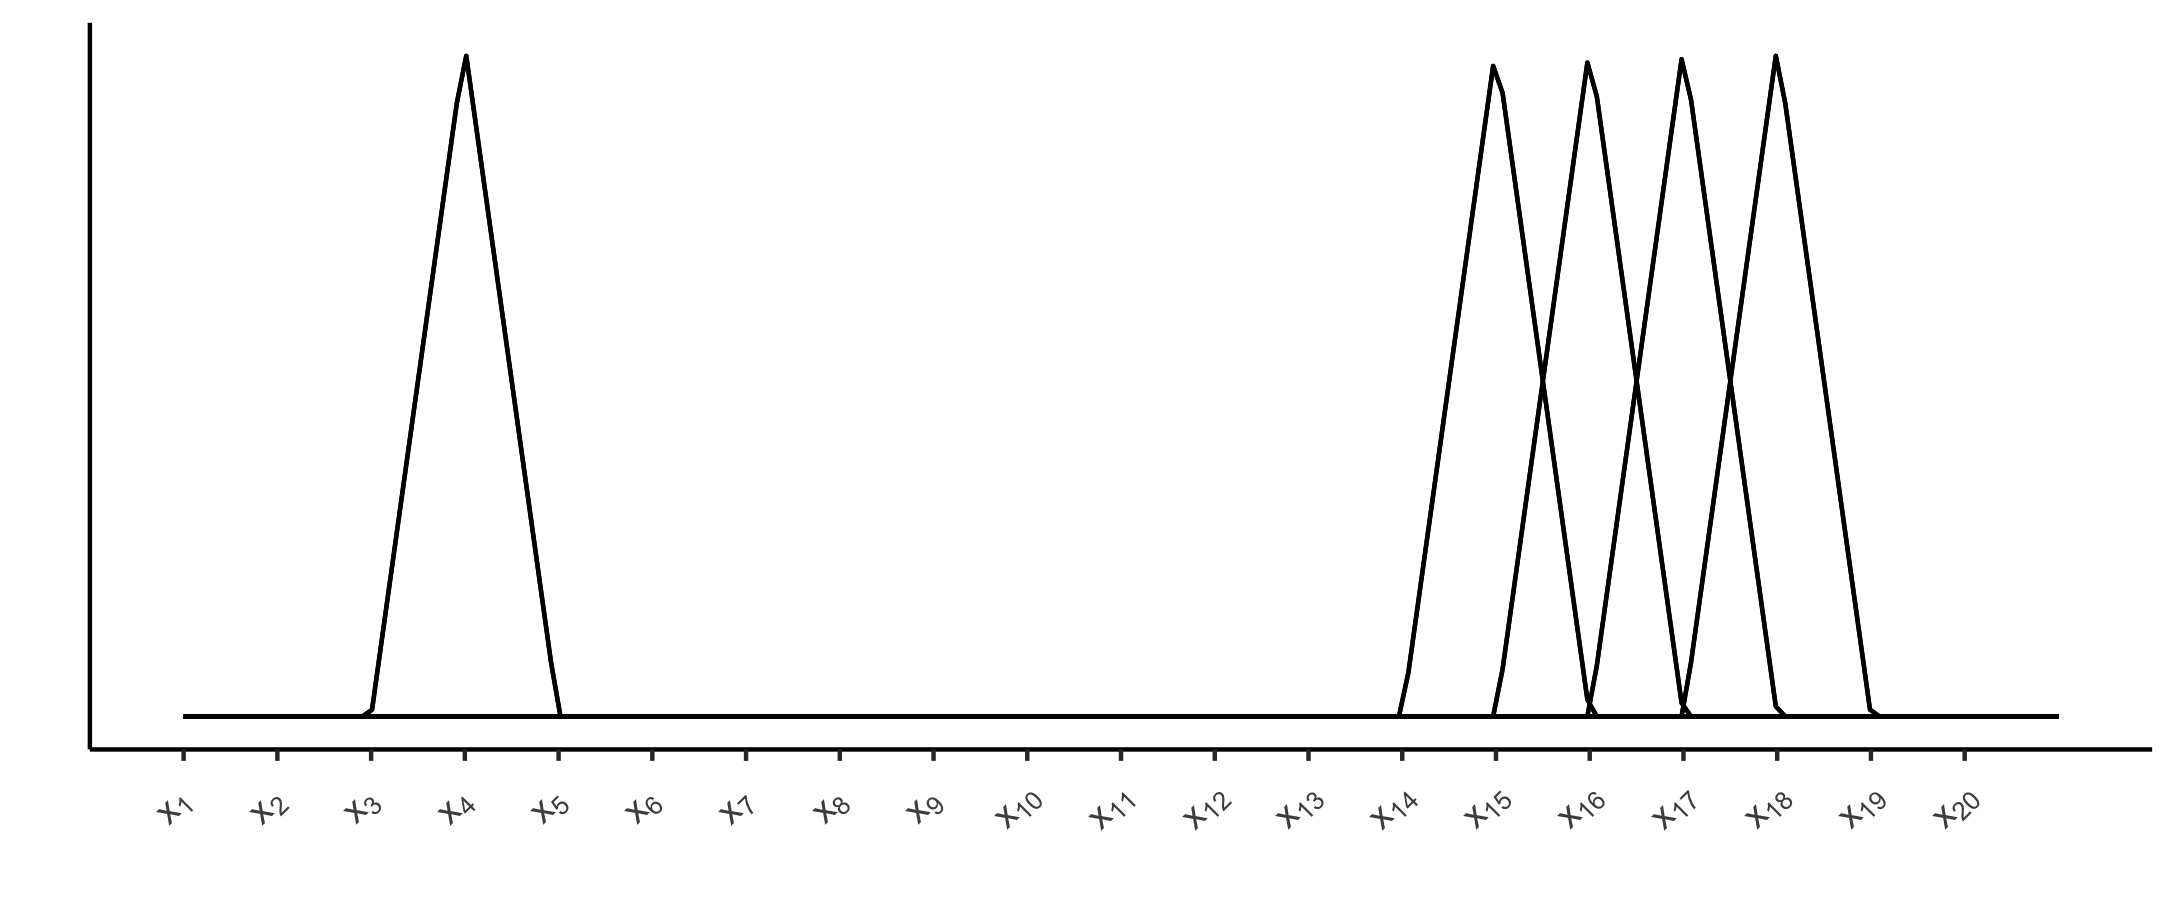
\includegraphics[width=0.75\textwidth]{img/uni_linear_bsplines}
 \caption{\textit{of degree 1} }\label{fig:overlapping-linear-bsplines}
  \end{subfigure}
   \end{center}
  \hfill
  \begin{center}
 \begin{subfigure}[t]{0.75\textwidth}
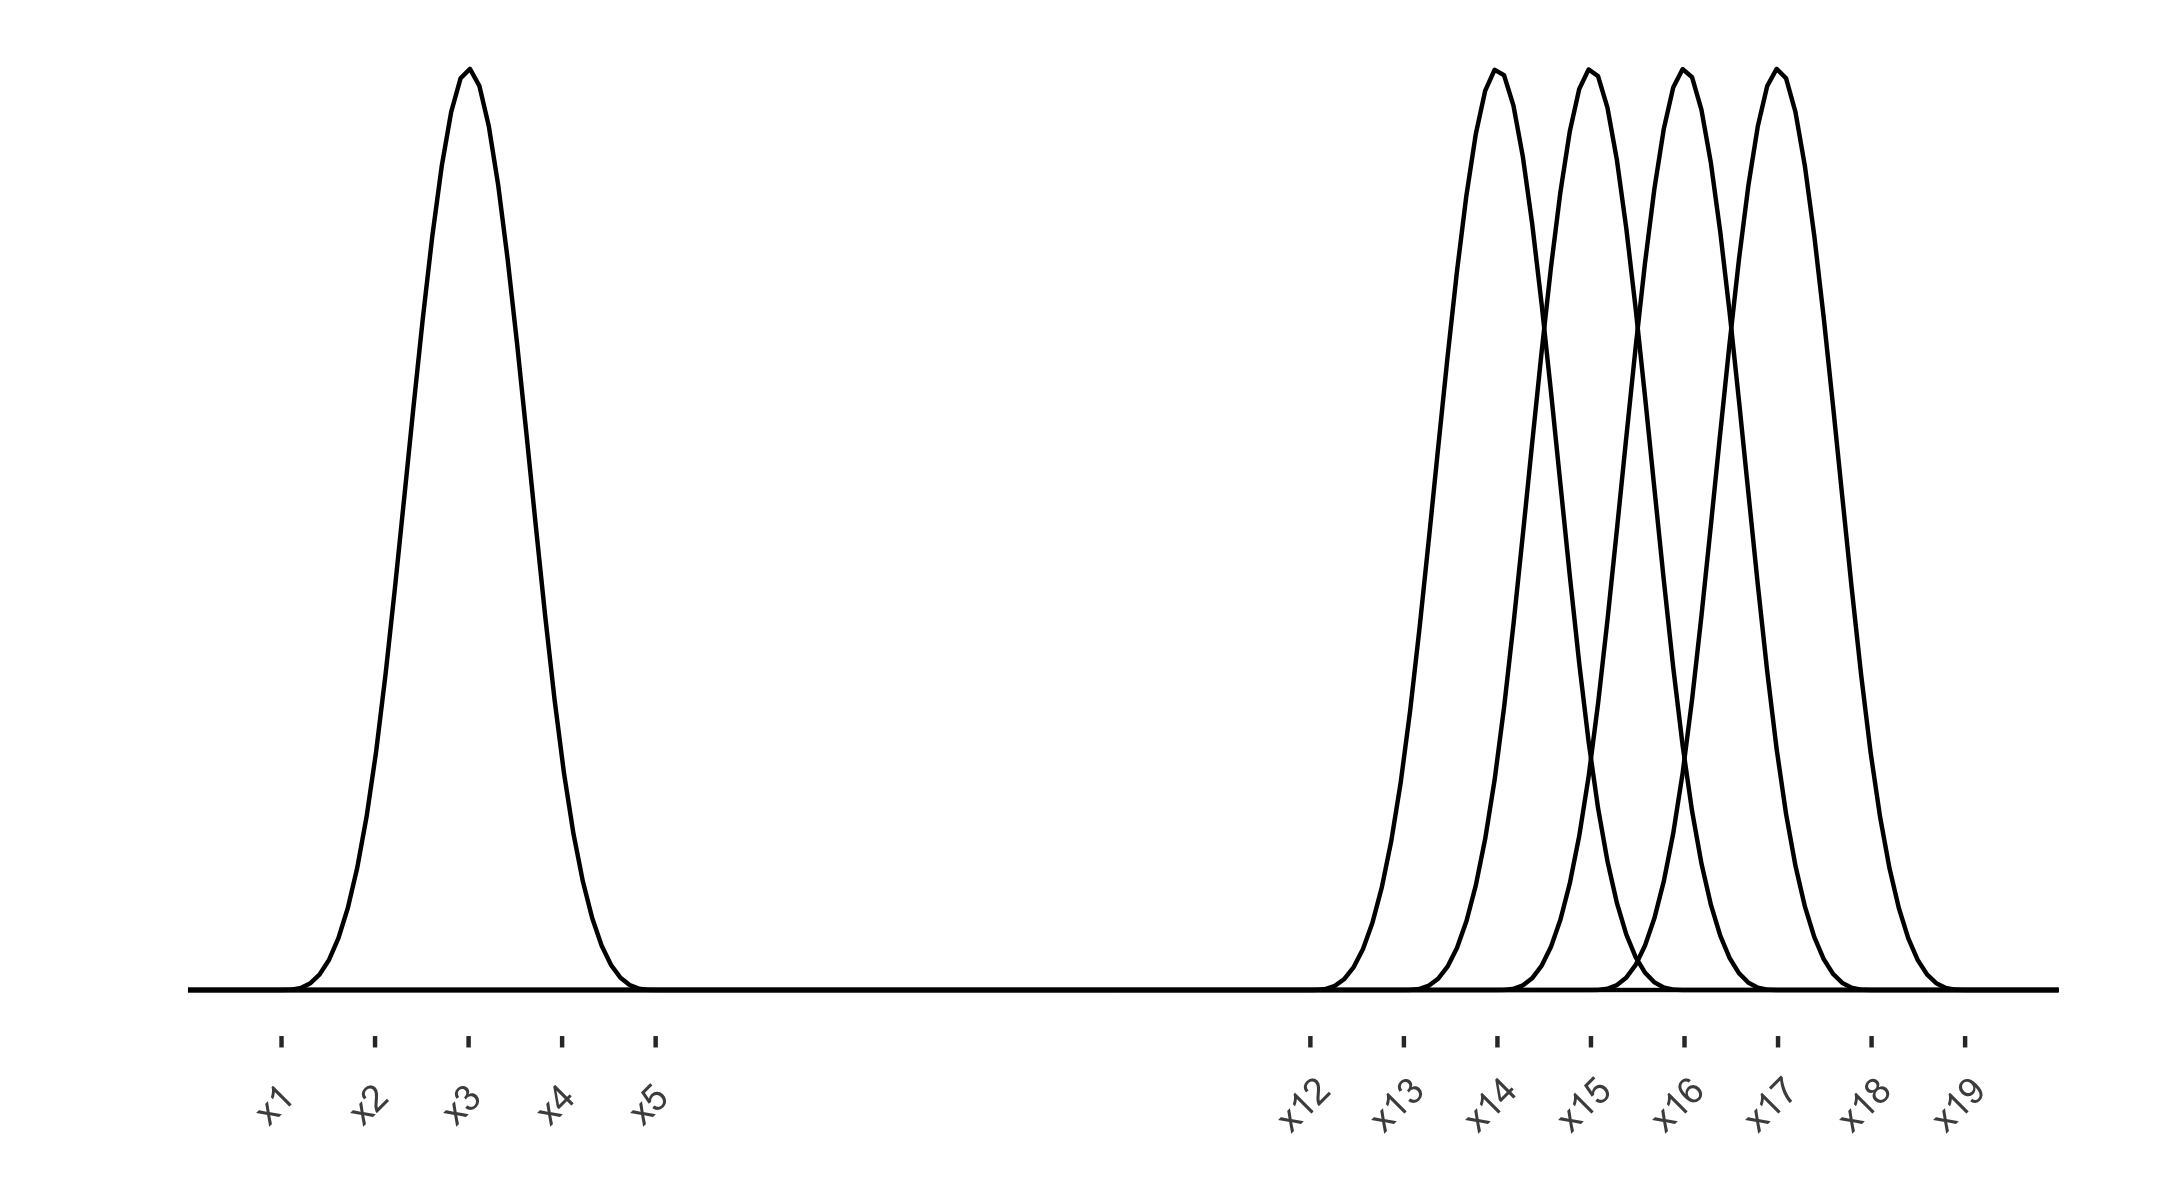
\includegraphics[width = \textwidth]{img/uni_cubic_bsplines}
 \caption{\textit{of degree 2}}
\label{fig:overlapping-cubic-bsplines}
 \end{subfigure}
 \end{center}
\end{figure}

B-splines make attractive basis functions for nonparametric regression; a linear combination of B-spline basis functions gives a smooth curve. Once a B-spline basis is computed, their application is no more difficult than polynomial regression, and extension to two-dimensional smoothing is available with the use of tensor products. To construct a B-spline representation for $\phi$, we need to equip the $l$ and $m$ axes each with a B-spline basis: let

\[
B_{l,1}\left(l\right),\dots, B_{l,K_1}\left(l\right)  \mbox{ and } B_{m,1}\left(m\right),\dots, B_{m,K_2}\left(m\right)
\]
\noindent
denote the B-spline bases for $l$ and $m$, each having a set of equally spaced knots along their respective domain. It is worth noting that one is free to specify a different basis for each dimension either by using different order B-spline or, of course, using different numbers of knots. The tensor product basis functions
\begin{equation*}
T_{kk'}\left(l,m\right) = B_{l,k}\left(l\right){B}_{m,k'}\left(m\right)
\end{equation*}
\noindent
carve the $l$-$m$ domain into rectangles. Figure~\ref{fig:bicubic-bspline-function} shows a single $T_{kk'}$, where the marginal B-spline bases are of degree 2. For a given knot grid, we can approximate a surface, $\phi$, by

\begin{equation} \label{eq:tensor-product-bspline-expansion-phi}
\phi\left(l,m\right) = \sum_{i=1}^{k_1} \sum_{j=1}^{k_2} \theta_{ij} B_{l,i}\left(l\right) B_{m,j}\left(m\right). 
\end{equation}
\noindent
Substituting this expression for $\phi$ in the negative log likelihood \eqref{eq:full-joint-likelihood} gives
\begin{equation} \label{eq:full-joint-likelihood-BS}
-2\ell\left(\theta_{11},\dots, \theta_{k_1,k_2} \vert Y_1,\dots, Y_N, \sigma^2\right)  = \sum_{i=1}^N \sum_{j=2}^{p_i} \log\sigma_{ij}^2 +  \sum_{i=1}^N \sum_{j=2}^{p_i} \frac{1}{\sigma^{2}_{ij}}\left( y_{ij} - \sum_{k<j}\left[ \sum_{i'=1}^{k_1} \sum_{j'=1}^{k_2} \theta_{i'j'} B_{l,i'}\left(l_{ijk}\right) B_{m,j'}\left(m_{ijk}\right)\right] y_{ik}  \right)^2.
\end{equation}
% For fixed $\sigma^2$ as in \eqref{eq:penalized-joint-loglik-given-sigma}, we define the estimator of $\phi$ as the minimizer of 
%\begin{equation} 
%-2\ell\left(\phi \vert Y_1,\dots, Y_N\right) + \lambda J\left(\phi\right) = \sum_{i=1}^N \sum_{j=2}^{p_i} \sigma^{-2}_{ij}\left( y_{ij} - \sum_{k<j} \phi\left(\bfv_{ijk}\right) y_{ik}  \right)^2 + \lambda J\left( \phi \right),
%\end{equation} 
%\noindent
%where $J\left(\phi\right)$ is a penalty on the roughness of the fitted function. 
%
%
\begin{figure}[H]
  \caption{\textit{ Tensor product of two cubic B-splines }}\label{fig:bicubic-bspline-function}
    \begin{center}
 \begin{subfigure}[t]{0.48\textwidth}
  \centering
  \includegraphics[width=\textwidth]{img/bicubic_basis_function}
  \end{subfigure}
 \begin{subfigure}[t]{.48\textwidth}
  \centering
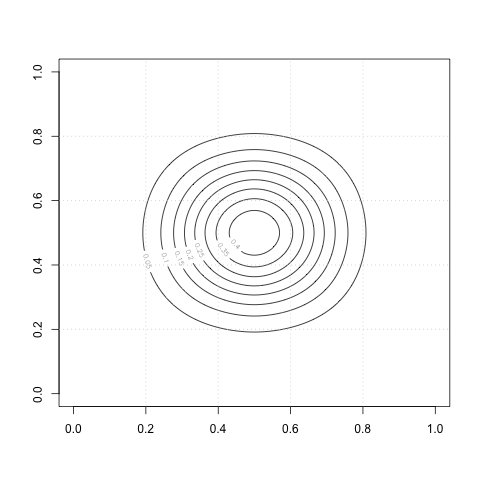
\includegraphics[width=\textwidth]{img/bicubic_bspline_contour}
 \end{subfigure}
 \end{center}
\end{figure}



%%%%%%%%%%%%%%%%%%%%%%%%%%%%%%%%%%%%%%%%%%%%%%%%%%%%%%%%%%%%%%%%%%%%%%%%%%%%%%%%%%%%%%%%%%%
%%%%%%%%%%%%%%%%%%%%%%%%%%%%%%%%%%%%%%%%%%%%%%%%%%%%%%%%%%%%%%%%%%%%%%%%%%%%%%%%%%%%%%%%%%%
%%%%%%%%%%%%%%%%%%%%%%%%%%%%%%%%%%%%%%%%%%%%%%%%%%%%%%%%%%%%%%%%%%%%%%%%%%%%%%%%%%%%%%%%%%%
%%%%%%%%%%%%%%%%%%%%%%%%%%%%%%%%%%%%%%%%%%%%%%%%%%%%%%%%%%%%%%%%%%%%%%%%%%%%%%%%%%%%%%%%%%%

\section{Difference penalties}

By using rich B-spline bases for $l$ and $m$ alongside discrete difference penalties on the spline coefficients, we can achieve as much smoothness of the fitted function in the $l$ and $m$ dimensions as desired. \cite{o1986statistical} was the first to propose using a rich B-spline basis alongside a penalty to restrict the flexibility of the fitted curve. He proposed the curvature penalty as defined for the cubic smoothing spline:
\begin{equation} \label{eq:second-derivative-penalty}
J = \int_0^1 \left( f^{\prime \prime}\left(x\right)\right)^2.
\end{equation}

\noindent
For a function that can be written as linear combination of B-spline basis functions, $\phi\left(v\right) = \sum\limits_{j=1}^k \theta_i B_j\left(v\right)$, one can derive a banded matrix $P$ using the properties of B-splines such that 
 \[
 J = \theta^\prime P \theta
 \] 
  \noindent
 where $\theta = \left(\theta_1,\dots, \theta_k\right)$ denotes the vector of B-spline basis coefficients. The $i$-$j^{th}$ element of the penalty matrix $P$ is given by
 
 \[
 p_{ij} = \int_0^1 B_i^{\prime \prime}\left(x\right) B_j^{\prime \prime}\left(x\right).
 \]
\cite{wand2008semiparametric} extend O'Sullivan's work to higher order derivatives for general degree B-splines and derive an exact matrix algebraic expression for the penalty matrices.  The computation of $P$ is nontrivial and becomes very tedious when the third and fourth derivative are used as the roughness measure. In the cubic case, the expression is a result of the application of Simpson's Rule applied to the inter-knot differences since each $B_i^{\prime \prime} B_j^{\prime \prime}$ is a piecewise quadratic function. The penalty may be written
 \[
 P = \left(B^{\prime \prime}\right)^\prime \textup{diag}\left(\omega \right) B^{\prime \prime}, 
 \]
 \noindent
 where $B^{\prime \prime}$ is the $3\left( k + 7 \right) \times \left( k + 4 \right)$ matrix with $i$-$j^{th}$ entry given by $B_j^{\prime \prime} \left(x_i^*\right)$, $x^*_i$ is the $i^{th}$ element of 
\[
\left( \phi_1,\frac{\phi_1+\phi_2}{2},\phi_2,\phi_2,\frac{\phi_2+\phi_3}{2},\phi_3,\dots,\phi_{k+7},\frac{\phi_{k+7}+\phi_{k+8}}{2},\phi_{k+8} \right),
\]
 \noindent
 and $\omega$ is the $3\left(k+7\right) \times 1$ vector given by
\begin{align*}
\omega &= \left( \frac{1}{6}\left(\Delta \phi \right)_1,\frac{4}{6}\left(\Delta \phi \right)_1, \frac{1}{6}\left(\Delta \phi \right)_1,\frac{1}{6}\left(\Delta \phi \right)_2, \frac{4}{6}\left(\Delta \phi \right)_2,  \right. \\
&\qquad   \left. {} \frac{1}{6}\left(\Delta \phi \right)_2 , \dots , \frac{1}{6}\left(\Delta \phi \right)_{n+7}, \frac{4}{6}\left(\Delta \phi \right)_{k+7}, \frac{1}{6}\left(\Delta \phi \right)_{k+7}  \right) \\
\end{align*}
\noindent
where $\left(\Delta \phi \right)_j = \phi_{j+1}-\phi_j$. They generalize this to the case of any order penalty and present a table of formulas for constructing any arbitrary penalty matrix, $P$.  

\bigskip

Alternatively, \cite{eilers1996flexible} proposed replacing the derivative-based penalty \eqref{eq:second-derivative-penalty} with a finite difference penalty on the B-spline coefficients. Using the properties of B-splines, it is straightforward to show that the difference penalty of order $d$ is a good discrete approximation to the integrated square of the $d^{th}$ derivative, so little is lost by using it in place of the derivative-based penalty. The $d^{th}$ order difference penalty is given by 
\begin{equation} \label{eq:bspline-difference-penalty-1}
J_d\left( \phi \right) = \sum_{j=d}^n \left(\Delta^d \theta_j\right)^2,
\end{equation} 
\noindent
Let $D_d$ denote the matrix difference operator:
\[
D_d\theta = \Delta^d \theta,
\]
\noindent
where $\Delta \theta_j = \theta_j - \theta_{j-1}$, and $\Delta^2 \theta_j = \Delta\left(\Delta \theta_j\right) = \theta_j - 2\theta_{j-1} + \theta_{j-2}$. In general,
\begin{equation*}
\Delta^d \theta_j = \Delta\left(\Delta^{d-1} \theta_j \right).
\end{equation*} 
\noindent
Then, \eqref{eq:bspline-difference-penalty-1} can be written in terms of the squared norm of the difference operator applied to the vector of B-spline coefficients:
\begin{align} 
\begin{split} \label{eq:bspline-difference-penalty-2}
J_d\left( f \right) &= \vert \vert D_d\theta \vert \vert^2 \\
&= \theta^\prime P_d \theta
\end{split}
\end{align}
\noindent
where $P_d = D_d^\prime D_d$.  To examine the connection between the second-derivative penalty to the penalty on second-order differences of the B-spline coefficients, we only need to employ straightforward calculus and exploit the recursive property of the B-spline basis functions. Consider a cubic B-spline 
\[
f = \sum_{i = 1}^k \theta_i B_{i,3}.
\]
The traditional smoothness penalty applied to $f$ is given by
\begin{equation*} 
\int_0^1 \left( f^{\prime \prime}\left(x\right)\right)^2\ = \int_{0}^{1} \left\{ \sum\limits_{j=1}^k  \theta_j B_{j,3}^{\prime \prime}\left(x\right) \right\}^2.
\end{equation*}
\noindent
The derivative properties of B-splines permits this to be written as 
\begin{equation*} \label{eq:second-derivative-bspline-penalty}
\int_0^1 \left[ f^{\prime \prime}\right]^2\ =  \int_{0}^{1}  \bigg[ \sum\limits_{i=1}^k \sum\limits_{j=1}^k \Delta^2 \theta_i \Delta^2 \theta_j B_{i,1}B_{j,1}\bigg]. 
\end{equation*}
\noindent
Most of the cross products of $B_{i,1}$ and $B_{j,1}$ vanish since B-splines of degree 1 only overlap when $j$ is $i-1$, $i$, or $i+1$. Thus, we have that
\begin{align}
\begin{split}
\int_0^1 \left( f^{\prime \prime}\left(x\right)\right)^2  = {} &  \int_0^1 \bigg[ \left( \sum\limits_{j=1}^k \Delta^2 \theta_j  B_j \right)^2  + 2 \sum_{j}\Delta^2 \theta_j\Delta^2 \theta_{j-1}B_{j,1}B_{j-1,1} \bigg]\\ 
= {} & \sum \limits_{j=1}^k  \left( \Delta^2\theta_j \right)^2 \int_0^1 B_{j,1}^2\ + 2 \sum\limits_{j=1}^k \Delta^2 \theta_j\Delta^2 \theta_{j-1} \int_0^1 B_{j,1}B_{j-1,1} 
\end{split}
\end{align}
\noindent
which can be written as
\begin{equation} \label{eq:derivative-penalty-difference-penalty-connection}
\int_0^1 \left( f^{\prime \prime}\left(x\right)\right)^2  = c_1 \sum\limits_{j=2}^k \left( \Delta^2 \theta_j\right)^2 + c_2 \sum\limits_{j=3}^n \Delta^2 \theta_j\Delta^2 \theta_{j-1}
\end{equation}
\noindent
Given a set of equidistant knots, the constants $c_1$ and $c_2$ are given by
\begin{equation}
\begin{split}
c_1 & =   \int_0^1 B_{j,1}^2\\
c_2 & = \int_0^1 B_{j,1}B_{j-1,1}.
\end{split}
\end{equation}
This establishes that traditional smoothness penalty on the squared second derivative can be written as a linear combination of a penalty on the second-order differences of the B-spline coefficients \ref{eq:bspline-difference-penalty-1} and the sum of the cross products of neighboring second differences. The second term in \ref{eq:derivative-penalty-difference-penalty-connection} leads to a complex objective function when minimizing the penalized likelihood, where seven adjacent spline coefficients occur, as opposed to five if only the first term in \ref{eq:derivative-penalty-difference-penalty-connection} is used in the penalty. The added complexity is a consequence of overlapping B-splines, which quickly increases when using higher order differences and higher order B-splines. We can seamlessly augment the likelihood with the difference penalty to achieve smooth fitted functions without the complexity posed by the derivative-based penalty.

\bigskip

A smoother sequence of coefficients leads to a smoother curve, as illustrated in Figure~\ref{fig:increasing-lambda-pspline-fits}.  The relationship between P-spline curves and their coefficients is easily characterized if we consider the coefficients as the skeleton of the function, and draping the B-splines over them puts the flesh on the bones, so to speak. As long as the coefficient sequence is smooth, the number of basis functions (and coefficients) is unimportant since the penalty ensures the smoothness of the skeleton and that the fitting procedure is well-conditioned.  

\begin{figure}[H] 
\begin{subfigure}{.4\textwidth}
  \centering
   \graphicspath{{img/}}
  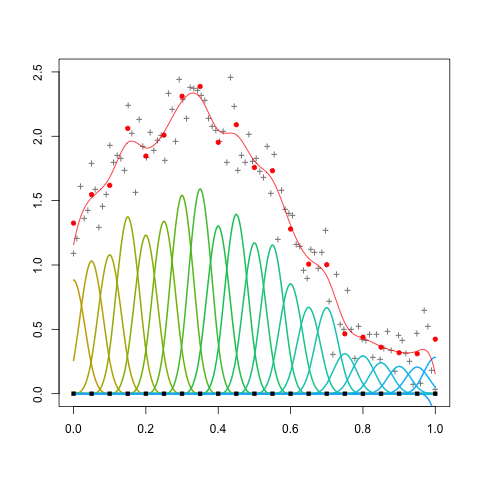
\includegraphics[scale=0.4]{pspline_pord2_xsmall_lambda.png}
  \label{fig:pspline_small_lambda}
\end{subfigure}
\begin{subfigure}{.5\textwidth}
  \centering
   \graphicspath{{img/}}
  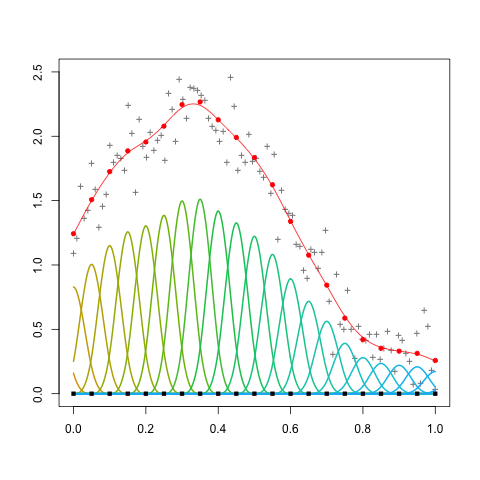
\includegraphics[scale=0.4]{pspline_pord2_small_lambda.png}
  \label{fig:pspline_small_lambda}
\end{subfigure}
\begin{subfigure}{.5\textwidth}
  \centering
   \graphicspath{{img/}}
  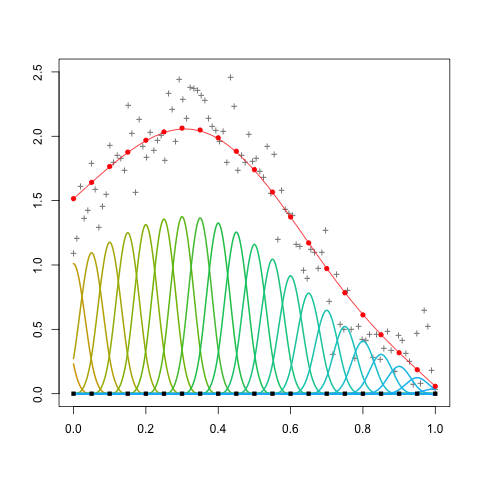
\includegraphics[scale=0.4]{pspline_pord2_medium_lambda.png}
  \label{fig:pspline_small_lambda}
\end{subfigure}
\begin{subfigure}{.5\textwidth}
  \centering
   \graphicspath{{img/}}
  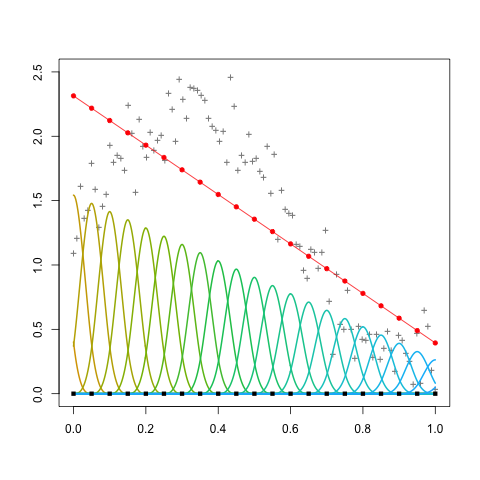
\includegraphics[scale=0.4]{pspline_pord2_large_lambda.png}
  \label{fig:pspline_small_lambda}
\end{subfigure}
\caption{\textit{Illustration of the impact of the second order difference penalty. The number of B-splines used is the same in each plot, with the value of the penalty parameter increasing from left to right and top to bottom across each plot. The red circles are the values of each of the B-spline coefficients; as the penalty increases, they form as smoother sequence as we move across the four plots, which results in a smoother fitted function. As the penalty parameter approaches infinity, the fit approaches a linear function as shown in the bottom right plot.}}
\label{fig:increasing-lambda-pspline-fits}
\end{figure}
P-splines can fit polynomial data exactly. If the true underlying function to be estimation is a polynomial in $l$ of degree $k$, then B-splines of degree $k$ or higher will fit the data perfectly. The proof of this requires a bit of mathematical labor and is left to Appendix~\ref{psplines-appendix}. Additionally, the limiting P-spline fit approaches a polynomial as the smoothing parameter tends to infinity.  As $\lambda \rightarrow \infty$, under a difference penalty of order $d$, the fitted function will approach a polynomial of degree $d-1$ as long as the degree of the B-splines is greater than or equal to $k$. Figure~\ref{fig:PS-difference-order-demo} demonstrates the impact of the order of the penalty on the fitted function as the smoothing parameter increases. To verify this mathematically, we need to use the relationship between the differenced coefficient sequence and the derivative of a B-spline - see Appendix~\ref{psplines-appendix}. Consider using the second-order difference penalty; when $\lambda$ is large, the penalty dominates the penalized likelihood, so that the minimizer $\theta$ must be such that $\sum_{j=3}^k\left(\Delta^2\theta_j\right)^2$ is close to zero. Consequently, each of the individual second differences must also be nearly zero, and thus the second derivative of the fitted function must be close to zero over the entire domain.
\begin{figure}[H]
\begin{subfigure}{.5\textwidth}
  \centering
   \graphicspath{{img/}}
  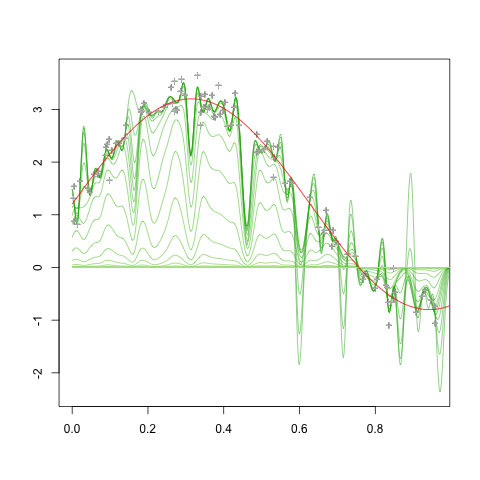
\includegraphics[scale=0.45]{PS_penalty_section_figure_6_order_0.png}
  %\label{fig:pspline_small_lambda}
\caption{$d=0$ }
\end{subfigure}
\begin{subfigure}{.5\textwidth}
  \centering
   \graphicspath{{img/}}
  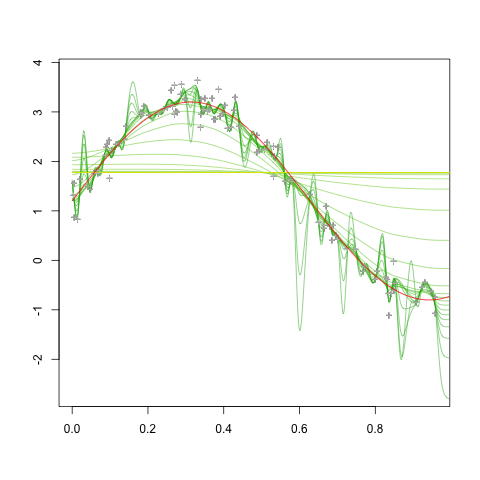
\includegraphics[scale=0.45]{PS_penalty_section_figure_6_order_1.png}
 % \label{fig:pspline_small_lambda}
\caption{$d=1$}
\end{subfigure}
\begin{subfigure}{.5\textwidth}
  \centering
   \graphicspath{{img/}}
  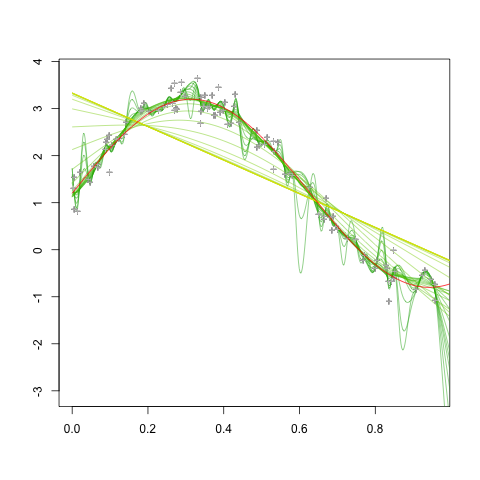
\includegraphics[scale=0.45]{PS_penalty_section_figure_6_order_2.png}
  %\label{fig:pspline_small_lambda}
\caption{$d=2$}
\end{subfigure}
\begin{subfigure}{.5\textwidth}
  \centering
   \graphicspath{{img/}}
  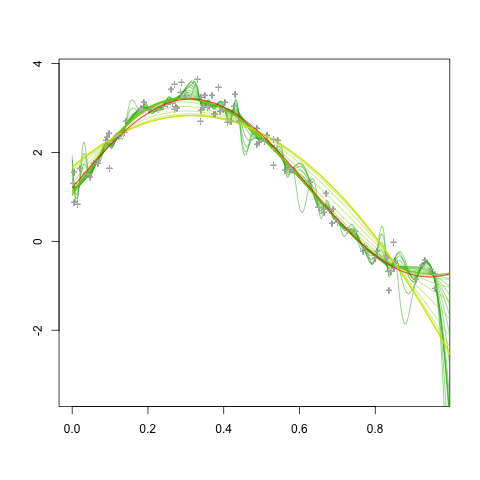
\includegraphics[scale=0.45]{PS_penalty_section_figure_6_order_3.png}
  %\label{fig:pspline_small_lambda}
\caption{$d=3$}
\end{subfigure}
\caption{\textit{Illustration of the impact of the order of the difference penalty. The number of B-splines used is the same in each plot, with the penalty parameter varying from across the same grid of values. The fitted curves in the upper left plot correspond to the difference penalty of order $0$, where $\vert D_0 \theta \vert^2 = \sum_{i} \theta_i^2$, analogous to ridge regression using the B-spline basis as regression covariates. The fitted curves approach polynomials of degree $d-1$ as $\lambda \rightarrow \infty$.}} \label{fig:PS-difference-order-demo}
\end{figure}


%%%%%%%%%%%%%%%%%%%%%%%%%%%%%%%%%%%%%%%%%%%%%%%%%%%%%%%%%%%%%%%%%%%%%%%%%%%%%%%%%%%%%%%%%%%
%%%%%%%%%%%%%%%%%%%%%%%%%%%%%%%%%%%%%%%%%%%%%%%%%%%%%%%%%%%%%%%%%%%%%%%%%%%%%%%%%%%%%%%%%%%
%%%%%%%%%%%%%%%%%%%%%%%%%%%%%%%%%%%%%%%%%%%%%%%%%%%%%%%%%%%%%%%%%%%%%%%%%%%%%%%%%%%%%%%%%%%
%%%%%%%%%%%%%%%%%%%%%%%%%%%%%%%%%%%%%%%%%%%%%%%%%%%%%%%%%%%%%%%%%%%%%%%%%%%%%%%%%%%%%%%%%%%
%%%%%%%%%%%%%%%%%%%%%%%%%%%%%%%%%%%%%%%%%%%%%%%%%%%%%%%%%%%%%%%%%%%%%%%%%%%%%%%%%%%%%%%%%%%
%%%%%%%%%%%%%%%%%%%%%%%%%%%%%%%%%%%%%%%%%%%%%%%%%%%%%%%%%%%%%%%%%%%%%%%%%%%%%%%%%%%%%%%%%%%
%%%%%%%%%%%%%%%%%%%%%%%%%%%%%%%%%%%%%%%%%%%%%%%%%%%%%%%%%%%%%%%%%%%%%%%%%%%%%%%%%%%%%%%%%%%
%%%%%%%%%%%%%%%%%%%%%%%%%%%%%%%%%%%%%%%%%%%%%%%%%%%%%%%%%%%%%%%%%%%%%%%%%%%%%%%%%%%%%%%%%%%

\section{The P-spline Estimator of the Generalized Autoregressive Varying Coefficient}

To extend the use of the difference penalty \eqref{eq:bspline-difference-penalty-1} to the bivariate setting, the only necessary modification to the one-dimensional differencing procedure is the addition of a second difference penalty, one for each variable $l$ and $m$. The explicit form of the minimizer of the penalized log likelihood is available, but for exposition, we first need to establish some notation. The smooth varying coefficient function $\phi$ evaluated at a $n_1 \times n_2$ grid of points over the $l \times m$ plane may be written 
\begin{equation*} 
\vphistar = B_2 \Theta B'_1
\end{equation*}
\noindent 
where $B_1$ is the $n_1 \times k_1$ matrix with $i^{th}$ column equal to the $i^{th}$ B-spline basis function for $l$ evaluated at the grid points $l_1,\dots l_{n_1}$,  $B_2$ is the $n_2 \times k_2$ matrix with $j^{th}$ column equal to the $j^{th}$ B-spline basis function for $m$ evaluated at the grid points $m_1,\dots m_{n_2}$. The matrix $\Theta$ denotes the $k_1 \times k_2$ matrix of tensor product coefficients, with elements $\theta_{ij}$. Smoothing $\phi$ in the $l$ direction can be achieved by applying a difference penalty to the rows of $\Theta$, and similarly in the $m$ direction by applying a difference penalty to the columns. We take $\phi_\lambda$ to be the minimizer of 
\begin{align} 
\begin{split}\label{eq:folded-difference-penalty-log-likelihood}
&-2\ell\left(\phi \vert Y_1,\dots, Y_N, \sigma^2\right) + J\left(\phi\right) = \sum_{i=1}^N \sum_{j=2}^{p_i} \sigma^{-2}\left({t_{ij}}\right) \left(y_{ij} - \sum_{k=1}^{j-1} \left( \sum_{r=1}^{k_1} \sum_{c=1}^{k_2} \theta_{rc} B_r\left(l_{ijk}\right)B_c\left(m_{ijk}\right)\right)y_{ik} \right)^2 \\ 
&\phantom{{}-2\ell\left(\phi \vert Y_1,\dots, Y_N\right) + J\left(\phi\right) = {}} + \lambda_l \sum_{r=1}^{k_1} \vert D_{d_{\ms l}} \theta_{r \cdot} \vert^2 + \lambda_m \sum_{c=1}^{k_2} \vert D_{d_{\ms m}} \theta_{\cdot c} \vert^2.
\end{split}
\end{align}
\noindent
where $\theta_{r \cdot}$ and $\theta_{\cdot c}$ denote the $r^{th}$ row and $c^{th}$ column of $\Theta$, respectively. The first term in \ref{eq:folded-difference-penalty-log-likelihood} imposes a difference penalty of order $d_{\ms l}$ on the rows of the coefficient matrix while the second term places a difference penalty (of possible different order $d_{\ms m}$) on the columns. We give each direction its own smoothing parameter to permit anisotropic smoothing; however, one could opt to use a single smoothing parameter for both directions and dodge the added work of optimizing the amount of smoothing with two separate parameters. 

\bigskip

The penalized log likelihood is quadratic in $\theta = \left(\theta_{11}, \dots, \theta_{k_1, k_2} \right)'$, and computation is quite simple if we express the coefficient matrix in ``unfolded'' notation. This allows us to express the varying coefficient function at the observed within-subject pairs of observation times as in the usual multiple regression form:
\begin{equation*}
\mbox{vec}\left\{\phi\left( \bfv \right)\right\} = B \theta
\end{equation*}
\noindent
Stacking the columns of $\Theta$ gives the vectorized coefficient matrix $\theta = \mbox{vec}\left( \Theta \right)$. The $\vert V \vert \times k_1 k_2$ tensor product basis $B$ is constructed from the tensor product of the marginal B-spline bases defined in \citet{eilers2006fast} as the \textit{row-wise Kronecker product} of the individual bases:
\begin{equation} \label{eq:rowwise-kronecker-product}
B = B_2 \square B_1 = \left( B_2 \otimes 1^\prime_{k_2} \right) \odot \left(1^\prime_{k_1} \otimes  B_1  \right).
\end{equation}
\noindent
The operator $\odot$ denotes the element-wise matrix product; $1_{k_1}$ ($1_{k_2}$) denotes the column vector of ones having length $k_1$ ($k_2$.) The operations in \eqref{eq:rowwise-kronecker-product} construct $B$ such that the $i^{th}$ row of $B_2\square B_1$ is the Kronecker product of the corresponding rows of $B_2$ and $B_1$. The penalty in \eqref{eq:folded-difference-penalty-log-likelihood} can also be compactly expressed:
\begin{equation*} \label{eq:tensor-product-penalty}
\lambda_l \vert \vert P_l \theta \vert \vert^2 + \lambda_m \vert \vert P_m \theta \vert\vert^2
\end{equation*}
\noindent
where $P_l = I_{k_2} \otimes D'_{d_{\ms l}} D_{d_{\ms l}} $ and $P_m =  D'_{d_{\ms m}} D_{d_{\ms m}} \otimes I_{k_1}$. We define $Y$, the vector of stacked subject-specific vectors,  as before, and the matrix $X$ of autoregressive covariates as previously \eqref{eq:ar-design-matrix-1} so that \eqref{eq:folded-difference-penalty-log-likelihood} can be written in matrix form as
\begin{equation} \label{eq:tensor-pspline-objective-function}
-2\ell\left(\phi \vert Y_1,\dots, Y_N\right) + J\left(\phi\right) = \left( Y - XB\theta\right)^\prime D^{-1}\left( Y - XB\theta\right)  + \lambda_l\vert\vert P_l \theta \vert\vert^2 + \lambda_m \vert\vert P_m \theta\vert \vert^2,
\end{equation}
\noindent
with $\hat{\theta}$ solving the system of equations 
\begin{equation} \label{eq:tensor-pspline-normal-equations}
\left[ \left(XB\right)^\prime D^{-1} XB +  \lambda_l P_l+ \lambda_m P_m\right]\theta = \left(X B\right)^\prime D^{-1}Y.
\end{equation}

\noindent
From \eqref{eq:tensor-pspline-normal-equations}, we note that the system of equations depends on basis coefficients remains fixed at $k_1 k_2$, even as the number of observations increases. The grid of regression coefficients can be recovered by arranging the elements of $\hat{\theta}$ into a matrix of $k_1$ columns having length $k_2$. The vector of fitted values is given by 

\begin{align}
\begin{split} \label{eq:pspline-smoothing-matrix}
\hat{Y} &= X \left[ \left(XB\right)^\prime D^{-1} XB +  \lambda_l P_l+ \lambda_m P_m\right] \left(X B\right)^\prime D^{-1}Y\\
&= AY
\end{split}
\end{align}

\noindent
where $A = X \left[ \left(XB\right)' D^{-1} XB +  \lambda_l P_l+ \lambda_m P_m\right] \left(X B\right)' D^{-1}$ is the ``smoothing'' matrix, analogous to the smoothing matrix $\tilde{A}$ \eqref{eq:smoothing-matrix-A-tilde} for the smoothing spline estimator in Chapter~\ref{SSANOVA-chapter}. Its use in smoothing parameter selection and model tuning is similar to the reproducing kernel Hilbert space framework, which we will discuss in the next section.

\bigskip

This recipe for constructing a tensor product basis for $\phi$ is an easy and convenient way to construct a two-dimensional basis for a bivariate function with domain corresponding to the unit square. However, the domain autoregressive coefficient function, $\phi$, lies on the lower triangle of the unit square $0 < s < t < 1$:

\begin{figure}[H] \label{fig:triangle-domain}
    \graphicspath{{img/}}
 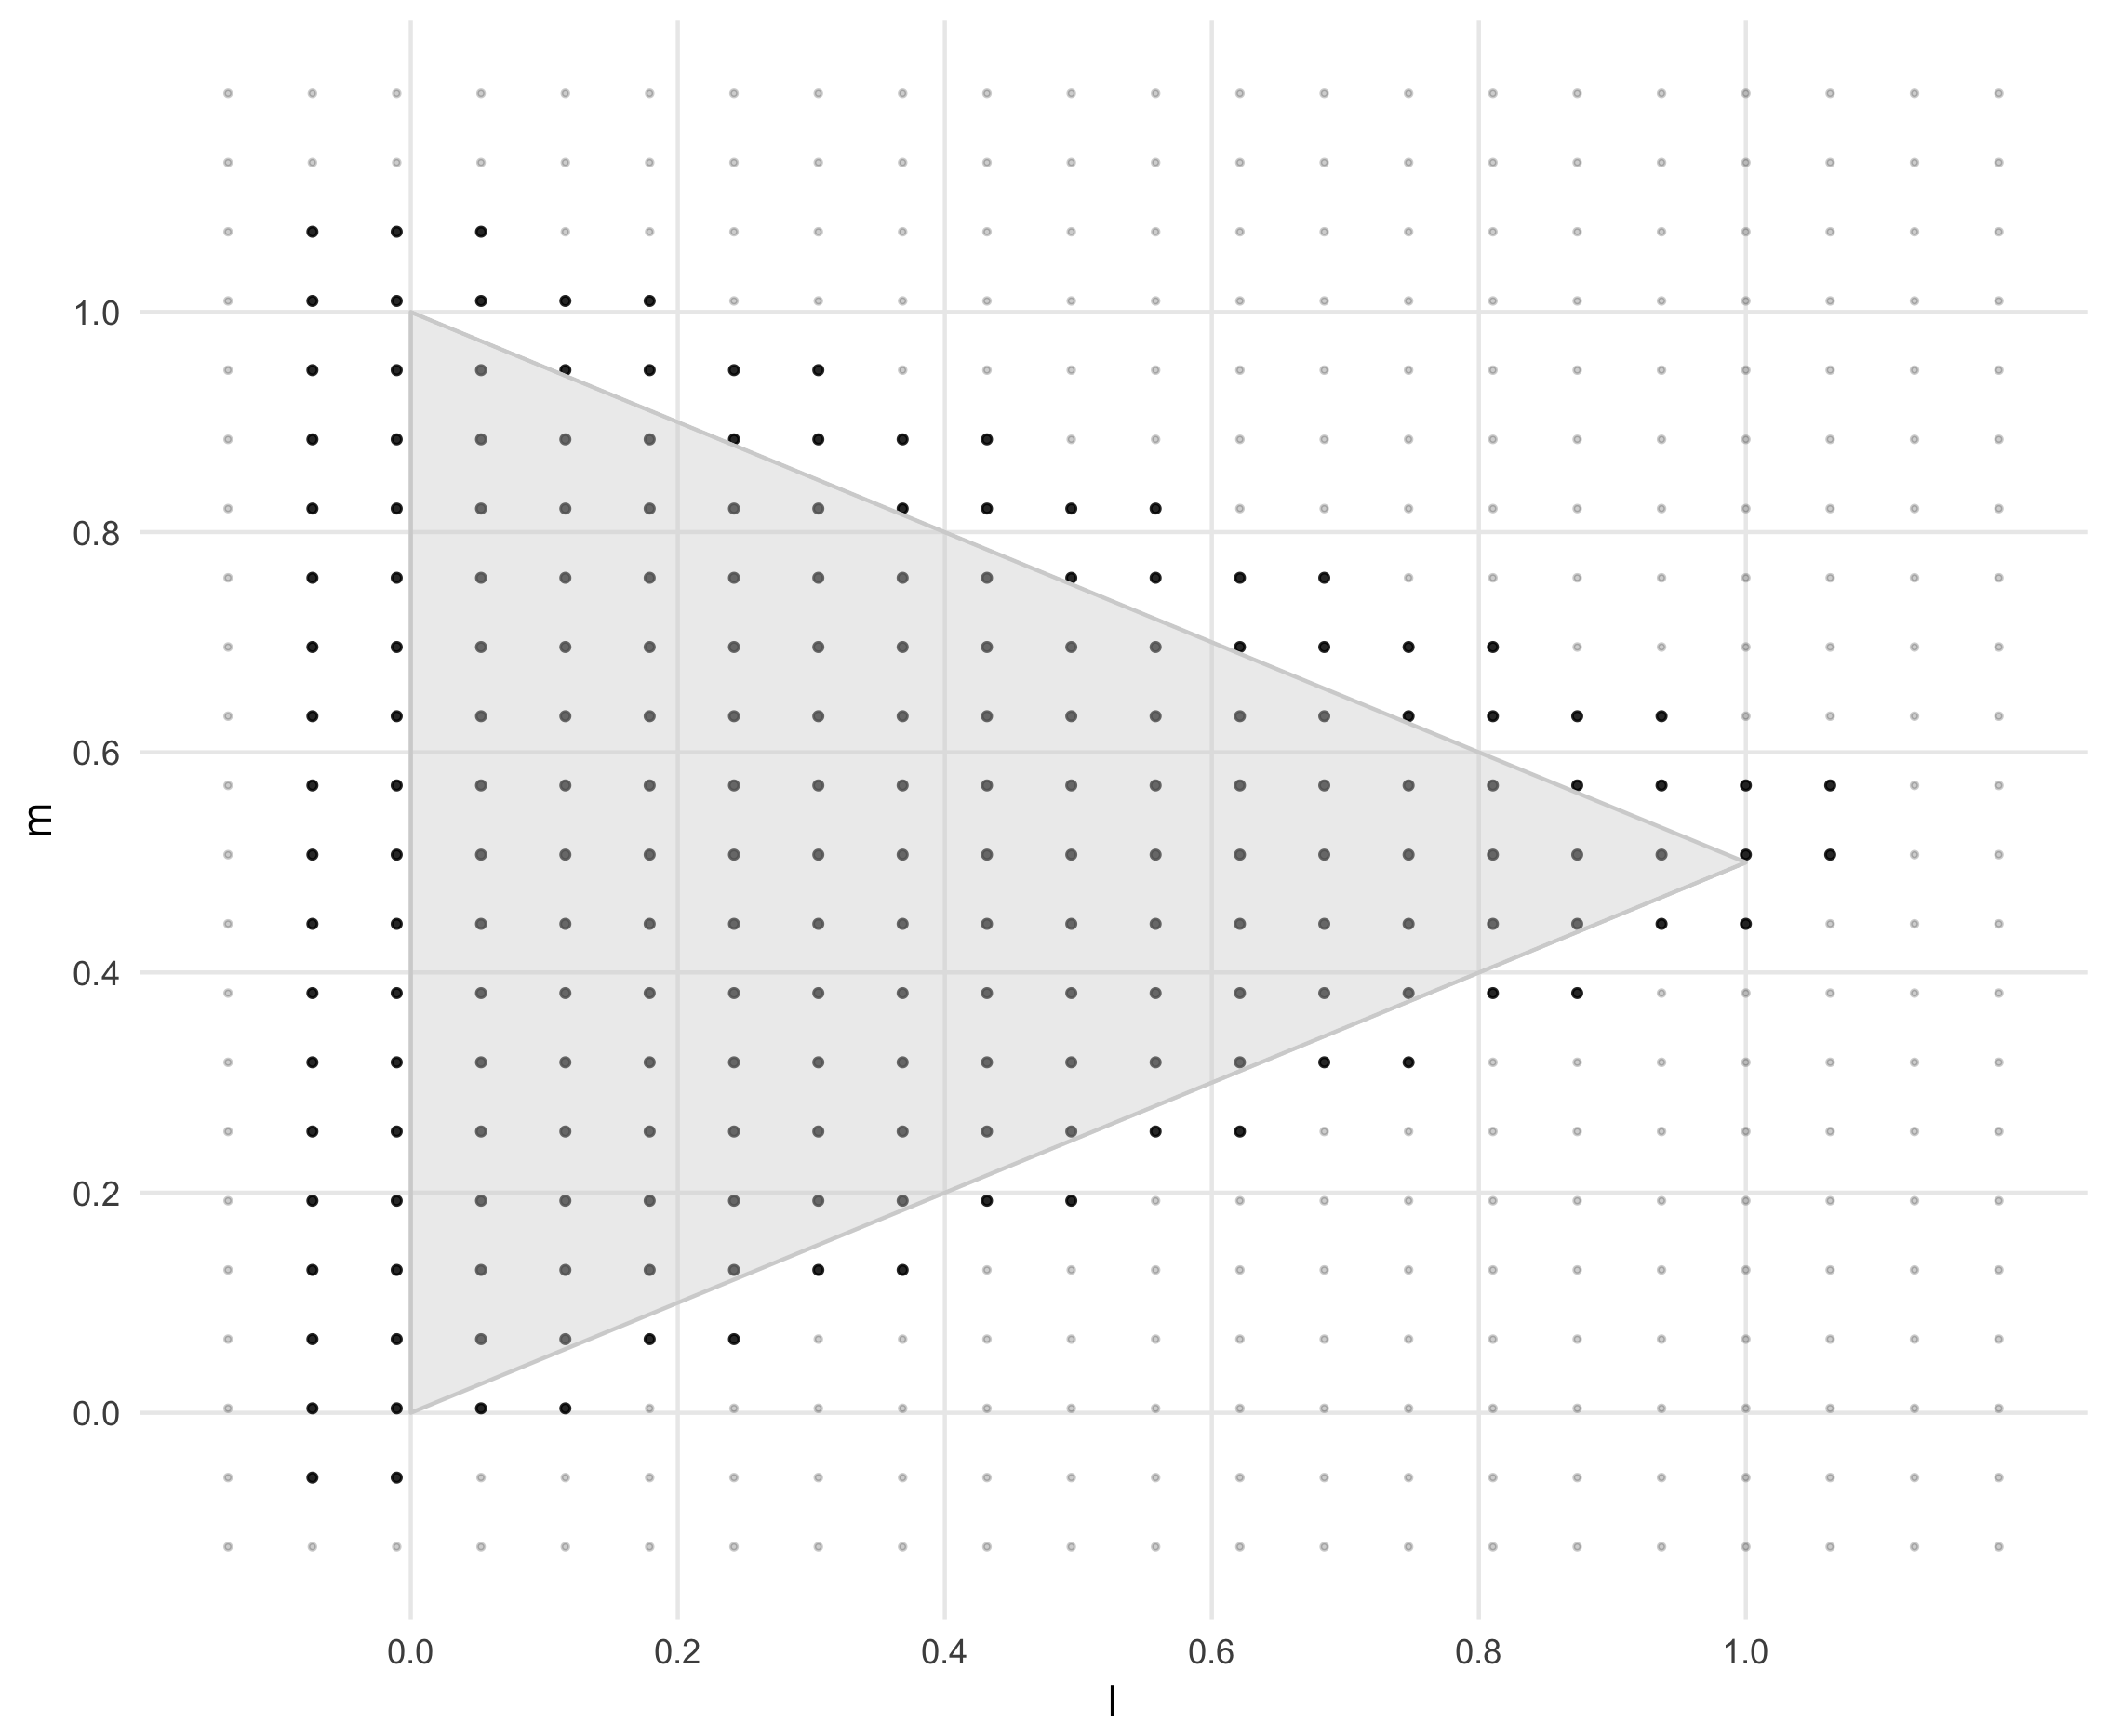
\includegraphics[scale=0.2]{knot-removal-on-triangle-domain.png}
 \caption{$\frac{l}{2} < m < 1 - \frac{l}{2}, \quad 0 < l < 1.$}
 \end{figure}


When the tensor product basis is constructed on the regular grid defined by the cartesian product of the knots of the marginal bases $B_1$ and $B_2$, a large number of basis functions anchored are at knots near which we have no data, so there is little information about the corresponding basis coefficient. As a result, the resulting tensor product matrix can be ill-conditioned and solving \eqref{eq:tensor-pspline-normal-equations} results in singularities. In this case, the quality of the estimator can suffer terribly. To correct for this instability, one can simply remove the knots corresponding to tensor products functions which do not overlap with the function domain from the basis, $B$, and trimming the penalty matrices $P_l$ and $P_m$ as needed. With the trimmed basis and penalties, optimization can be carried out as previously discussed. Alternatively, one could employ the use of multidimensional B-splines for the construction of the basis for $\bfv = \left(l,m\right)$. There is little about multidimensional splines in the Statistics literature - likely because the computational complexity associated with these methods, however, some in the field of computer graphics have proposed the use of their use for smoothing over arbitrary function domains, which are approximated by triangulations. See \citet{dahmen1992blossoming} and \citet{seidel1991symmetric} for details. 

%%%%%%%%%%%%%%%%%%%%%%%%%%%%%%%%%%%%%%%%%%%%%%%%%%%%%%%%%%%%%%%%%%%%%%%%%%%%%%%%%%%%%%%%%%%
%%%%%%%%%%%%%%%%%%%%%%%%%%%%%%%%%%%%%%%%%%%%%%%%%%%%%%%%%%%%%%%%%%%%%%%%%%%%%%%%%%%%%%%%%%%
%%%%%%%%%%%%%%%%%%%%%%%%%%%%%%%%%%%%%%%%%%%%%%%%%%%%%%%%%%%%%%%%%%%%%%%%%%%%%%%%%%%%%%%%%%%
%%%%%%%%%%%%%%%%%%%%%%%%%%%%%%%%%%%%%%%%%%%%%%%%%%%%%%%%%%%%%%%%%%%%%%%%%%%%%%%%%%%%%%%%%%%
%%%%%%%%%%%%%%%%%%%%%%%%%%%%%%%%%%%%%%%%%%%%%%%%%%%%%%%%%%%%%%%%%%%%%%%%%%%%%%%%%%%%%%%%%%%
%%%%%%%%%%%%%%%%%%%%%%%%%%%%%%%%%%%%%%%%%%%%%%%%%%%%%%%%%%%%%%%%%%%%%%%%%%%%%%%%%%%%%%%%%%%
%%%%%%%%%%%%%%%%%%%%%%%%%%%%%%%%%%%%%%%%%%%%%%%%%%%%%%%%%%%%%%%%%%%%%%%%%%%%%%%%%%%%%%%%%%%
%%%%%%%%%%%%%%%%%%%%%%%%%%%%%%%%%%%%%%%%%%%%%%%%%%%%%%%%%%%%%%%%%%%%%%%%%%%%%%%%%%%%%%%%%%%


%%==============================================================================================================================================
%%==============================================================================================================================================
%%==============================================================================================================================================
%%==============================================================================================================================================
%%==============================================================================================================================================
%%%==============================================================================================================================================


%%==============================================================================================================================================
%%==============================================================================================================================================
%%==============================================================================================================================================
%%==============================================================================================================================================
%%==============================================================================================================================================
%%==============================================================================================================================================

%%==============================================================================================================================================
%%==============================================================================================================================================
%%==============================================================================================================================================
%%==============================================================================================================================================
%%==============================================================================================================================================
%%==============================================================================================================================================

%\subsection{The reguarlized MLE for $\phi$ via tensor product P-splines}
%% \subfile{chapter-3-subfiles/chapter-3-tensor-product-pspline-MLE}
%To extend the P-spline framework to allow estimation of a bivariate function, $\phi$, we simply need to equip the $l$ and $m$ axes each with a B-spline basis. A basis for the varying coefficient function is constructed taking the tensor product of the two marginal bases. Let 
%\[
%B_{1}\left(l\right),\dots, B_{K}\left(l\right)  \mbox{ and } B_{1}\left(m\right),\dots, B_{L}\left(m\right)
%\]
%denote the B-spline bases for $l$ and $m$, each having a set of equally spaced knots along their respective domain. It is worth noting that while we have chosen not to distinguish between $\left\{ B_k \right\}$ and $\left\{ {B}_l \right\}$ for the sake of brevity, one is free to specify a different basis for each dimension either by using different order B-spline or, of course, using different numbers of knots, and hence entirely different knot sequences since P-splines rely on bases with equally spaced knots. The tensor product basis functions
%\begin{equation*}
%T_{jk}\left(l,m\right) = B_j\left(l\right){B}_k\left(m\right)
%\end{equation*}
%\noindent
%carve the $l$-$m$ domain into rectangles.  Figure~\ref{fig:sparse_bicubic_BS_basis} shows a thinned tensor product basis $\left\{ T_{kl} \right\}$; a portion of the basis was omitted to eliminate overlapping of the basis functions so that the reader can identify individual tensor products. Each ``hill'' in Figure~\ref{fig:sparse_bicubic_BS_basis} is associated with an unknown coefficient $\theta_{ij}$ which determines the height of the hill. For a given knot grid, we can approximate a surface by
%
%\begin{equation} \label{eq:varying-coefficient-tensor-product-expansion}
%\phi\left(l,m\right) = \sum_{i=1}^K \sum_{j=1}^L \theta_{ij} B_{i}\left(l\right) B_{j}\left(m\right), 
%\end{equation}
%\noindent
%and the function evaluated at the observed $\left(l_{ijk}, m_{ijk}\right)$ may be written 
%\begin{equation*} 
%\vphistar = B_m \Theta B_l^\prime
%\end{equation*}
%\noindent 
%where $\Theta$ denotes the $K \times L$ matrix of tensor product coefficients, with elements $\theta_{ij}$.
%
%\begin{figure}[H]
%\centering
% \graphicspath{{img/}}
%  \includegraphics[width=4in, height=4in]{bicubic_basis_function.png}
% 
%% 
% \subsection{Regularization with difference penalties} \label{subsection:univariate-psplines}
%
%The minimizer of \ref{eq:loglikelihood} honors the fidelity to the data, so to balance the complexity of the fitted function with the goodness of fit to the data, we can append a penalty to the negative log likelihood to control the fitted function. By using rich B-spline bases for $l$ and $m$ alongside discrete difference penalties on the spline coefficients, we can achieve as much smoothness of the fitted function in both the $l$ and $m$ dimensions as desired. \cite{o1986statistical} was the first to propose using a rich B-spline basis and using a penalty to restrict the flexibility of the fitted curve, like \cite{wahba1990spline} applying a penalty to the second derivative of the fitted curve:
%\[
%J = \int_0^1 \left[ f^{\prime \prime}\left(l\right)\right]^2\;dx.
%\]
%
%For a B-spline of the form
%\[
%f\left(x\right) = \sum\limits_{j=1}^n \theta_i B_j\left(x\right),
%\]
%one can derive a banded matrix $P$ using the properties of B-splines such that 
% \[
% J = \theta^\prime P \theta
% \] 
% \noindent
% where $\theta = \left(\theta_1,\dots, \theta_n\right)$. The $i$-$j^{th}$ element of $P$ is given by
% \[
% p_{ij} = \int_0^1 B_i^{\prime \prime} \left( x \right)B_j^{\prime \prime} \left( x \right)\;dx.
% \]

%As discussed in Section 2, we can define an entire class of functional autoregressive models using only the $l$ direction, and additionally, as discussed in Section 3, there is a natural expectation about the functional form of the autoregressive coefficient function (and hence covariance) as a function of $l$. The use of smoothing splines to estimate $\phi$ outlined in Section~\ref{} yields smooth null models, but smoothness of the elements of the Cholesky factor alone may not lead to desirable structure in the inverse covariance matrix.  

%
%These approaches implicitly adopt different notions of sparsity. Like \cite{huang2006covariance} and \cite{levina2008sparse}, our aim is to regularize the inverse of the covariance matrix through the Cholesky factor. Expressing the varying coefficient function using a tensor product basis expansion builds the foundation for a flexible estimation framework within which employing multiple notions of smoothness is simple and straightforward. 
%
%
%In some applications, it is useful to work with third and fourth order differences, since for large values of $\lambda$, the fitted curve approaches a parametric polynomial model. This may be of particular interest in the context of estimating the elements of the Cholesky factor, as many have proposed simple parametric functions of lag only for $\phi$, such as low order polynomials. See \cite{pourahmadi1999joint}. However, with the use of higher order derivatives, the computation of $P$ is nontrivial and becomes very tedious. \cite{eilers1996flexible} were the first to propose P-splines, or \emph{penalized B-splines}, as an approach to nonparametric regression. P-splines circumvent complexity associated with constructing such penalty matrices by omitting derivatives and integrals altogether, replacing them with finite differences and sums. 
%
%Instead, flexibility of the fitted function is controlled by using a discrete penalty matrix based on finite difference formulas. Smoothness of the fitted function is achieved by first using a rich B-spline basis with equally spaced knots to purposefully overfit the smooth coefficient vectors; this eliminates the difficulty of choosing the optimal set of knots. Then by attaching a difference penalty to the goodness of fit measure, one may prevent overfitting and make a potentially ill-conditioned fitting procedure a well-conditioned one. The finite difference penalty is simple to compute and can be handled mechanically for any order of the differences. Since it is easily introduced into regression equations, it is feasible to evaluate the impact of different orders of the differences on the fitted model.  Using the properties of B-splines, it is straightforward to show that the difference penalty of order $d$ is a good discrete approximation to the integrated square of the $d^{th}$ derivative, so little is lost by replacing the derivative-based penalty with
%
%\begin{equation} \label{eq:bspline-difference-penalty}
%J_d\left( f \right) = \sum_{j=d}^n \left(\Delta^d \theta_j\right)^2
%\end{equation} 
%\noindent
%where $\theta = \left( \theta_1,\dots,\theta_n \right)$. Let $D_d$ denote the matrix difference operator: $D_d\theta = \Delta^d \theta$, where
%
% \begin{align*}
% \Delta \theta_j &= \theta_j - \theta_{j-1}, \quad  \Delta^2 \theta_j = \Delta\left(\Delta \theta_j\right) = \theta_j - 2\theta_{j-1} + \theta_{j-2}
% \end{align*}
%\noindent 
%In general,
%\begin{equation*}
%\Delta^d \theta_j = \Delta\left(\Delta^{d-1} \theta_j \right).
%\end{equation*} 
%\noindent
%Then, \ref{eq:bspline-difference-penalty} can be written in terms of the squared norm of the difference operator applied to the vector of B-spline coefficients:
%\begin{align} 
%\begin{split} \label{eq:bspline-difference-penalty-vector-form}
%J_d\left( f \right) &= \vert \vert D_d\theta \vert \vert^2 \\
%&= \theta^\prime P_d \theta
%\end{split}
%\end{align}
%\noindent
%where $P_d = D_d^\prime D_d$.  To examine the connection between the second-derivative penalty to the penalty on second-order differences of the B-spline coefficients, we only need to employ straightforward calculus and exploit the recursive property of the B-spline basis functions:
%
%\begin{equation*} 
%\int_0^1 \left[ f^{\prime \prime}\left(x\right)\right]^2\;dx = \int_{0}^{1} \left\{ \sum\limits_{j=1}^n  \theta_j B_{j,3}^{\prime \prime} \left(l\right) \right\}^2\; dl.
%\end{equation*}
%\noindent
%The derivative properties of B-splines permits this to be written as 
%\begin{equation*} \label{eq:second-derivative-bspline-penalty}
%\int_0^1 \left[ f^{\prime \prime}\left(x\right)\right]^2\;dx =  \int_{0}^{1}  \bigg[ \sum\limits_{j=1}^n \sum\limits_{k=1}^n \Delta^2 \theta_j \Delta^2 \theta_k B_{j,1}\left(l\right)B_{k,1}\left(l\right)\bigg]\; dl  . 
%\end{equation*}
%\noindent
%Most of the cross products of $B_{j,1}\left(x\right)$ and $B_{k,1}\left( x \right)$ vanish since B-splines of degree 1 only overlap when $j$ is $k-1$, $k$, or $k+1$. Thus, we have that
%\begin{align}
%\begin{split}
%\int_0^1 \left[ f^{\prime \prime}\left(x\right)\right]^2\;dx  = {} &  \int_0^1 \bigg[ \left\{ \sum\limits_{j=1}^n   \Delta^2 \theta_j  B_j\left(l,1\right)  \right\}^2  + 2 \sum_{j}\Delta^2 \theta_j\Delta^2 \theta_{j-1}B_j\left(l,1\right)B_{j-1}\left(l,1\right) \bigg]\; dl \\ 
%= {} & \sum \limits_{j=1}^n  \left( \Delta^2\theta_j \right)^2 \int_0^1 B_j^2\left(l,1\right)\;dl \\
%   &{} \;\;\;\;\;\;\;\;\;\;\;\;\;\;\;\;\;\; + 2 \sum\limits_{j=1}^n \Delta^2 \theta_j\Delta^2 \theta_{j-1} \int_0^1 B_j\left(l,1\right)B_{j-1}\left(l,1\right)\;dl 
%\end{split}
%\end{align}
%\noindent
%which can be written as
%\begin{equation} \label{eq:derivative-penalty-difference-penalty-connection}
%\int_0^1 \left[ f^{\prime \prime}\left(x\right)\right]^2\;dx  = c_1 \sum\limits_{j=2}^n \left( \Delta^2 \theta_j\right)^2 + c_2 \sum\limits_{j=3}^n \Delta^2 \theta_j\Delta^2 \theta_{j-1}
%\end{equation}
%\noindent
%Given a set of equidistant knots, the constants $c_1$ and $c_2$ are given by
%\begin{equation}
%\begin{split}
%c_1 & =   \int_0^1 B_{j,1}^2\left(x\right) dx\\
%c_2 & = \int_0^1 B_{j,1}\left(x\right)B_{j-1,1}\left(x\right) dx.
%\end{split}
%\end{equation}
%
%This gives us that the traditional smoothness penalty on the squared second derivative can be written as a linear combination of a penalty on the second-order differences of the B-spline coefficients \ref{eq:bspline-difference-penalty} and the sum of the cross products of neighboring second differences. The second term in \ref{eq:derivative-penalty-difference-penalty-connection} leads to a complex objective function when minimizing the penalized likelihood, where seven adjacent spline coefficients occur, as opposed to five if only the first term in \ref{eq:derivative-penalty-difference-penalty-connection} is used in the penalty. The added complexity is a consequence of overlapping B-splines, which quickly increases when using higher order differences and higher order B-splines. We can seamlessly augment the likelihood with the difference penalty to achieve smooth fitted functions without the complexity posed by the derivative-based penalty.
%%citet{chen2011efficient}, citet{pourahmadi1999joint}, and citet{pourahmadi2002dynamic} have elicited parametric models for the generalized autoregressive coefficients, letting the GARPs depend only on the distance between two time points.
%
%A smoother sequence of coefficients leads to a smoother curve, as illustrated in Figure~\ref{fig:second_ord_PS_pen_SML_lambda}.  The relationship between P-spline curves and their coefficients is easily characterized if we consider the coefficients as the skeleton of the function, and draping the B-splines over them puts the flesh on the bones. As long as the coefficient sequence is smooth, the number of basis functions (and coefficients) is unimportant since the penalty ensures the smoothness of the skeleton and that the fitting procedure is well-conditioned. Figure~\ref{fig:overcomplete_basis_pspline} illustrates this utility of the penalty for simulated data; there are $m=10$ observations and $60$ cubic B-splines. This property of P-splines cannot be overly appreciated because it frees us from the concern of choosing the optimal set of knots. Unless computational constraints are of concern, which is possible with large models, it is prudent to use even more B-splines. Figure~\ref{fig:PS_penalty_section_figure_2} shows how the fitted function changes as the tuning parameter varies when the data are sparsely sampled. P-splines enjoy a number of additional advantageous properties, many of which are inherited from the attractive properties of B-splines. See \cite{eilers1996flexible}  for a detailed presentation. 
%
%\begin{figure}[H] \label{fig:PS-smoothing-figure-1}
%\begin{subfigure}{.5\textwidth}
%  \centering
%   \graphicspath{{img/}}
%  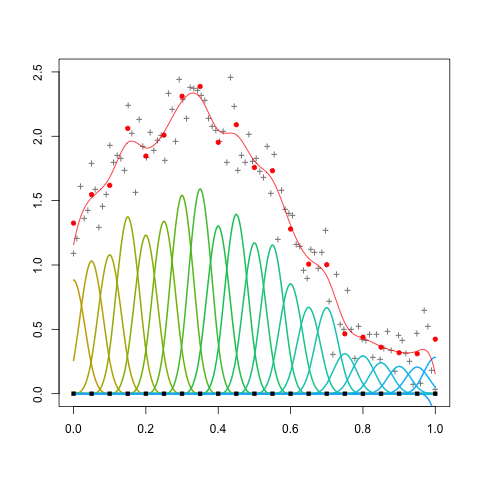
\includegraphics[scale=0.5]{pspline_pord2_xsmall_lambda.png}
%  \label{fig:pspline_small_lambda}
%\end{subfigure}
%\begin{subfigure}{.5\textwidth}
%  \centering
%   \graphicspath{{img/}}
%  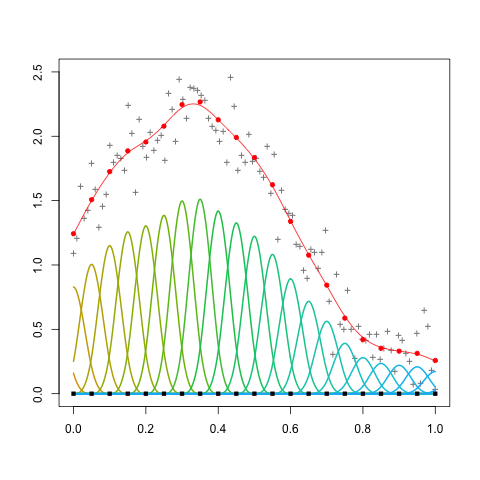
\includegraphics[scale=0.5]{pspline_pord2_small_lambda.png}
%  \label{fig:pspline_small_lambda}
%\end{subfigure}
%\begin{subfigure}{.5\textwidth}
%  \centering
%   \graphicspath{{img/}}
%  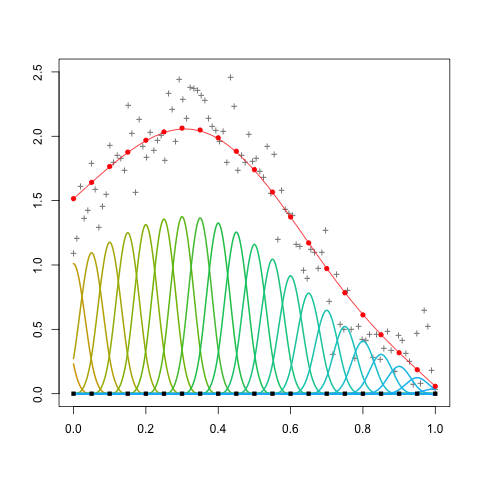
\includegraphics[scale=0.5]{pspline_pord2_medium_lambda.png}
%  \label{fig:pspline_small_lambda}
%\end{subfigure}
%\begin{subfigure}{.5\textwidth}
%  \centering
%   \graphicspath{{img/}}
%  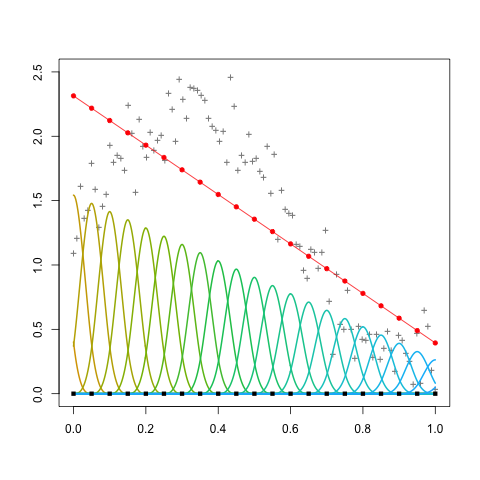
\includegraphics[scale=0.5]{pspline_pord2_large_lambda.png}
%  \label{fig:pspline_small_lambda}
%\end{subfigure}
%\caption{\textit{Illustration of the impact of the second order difference penalty. The number of B-splines used is the same in each plot, with the value of the penalty parameter increasing from left to right and top to bottom across each plot. The fitted curve in the upper left plot is the most ``wiggly'' of any of the fits, as the penalty plays the weakest roll in the fitted coefficients there. The red circles are the values of each of the B-spline coefficients; as the penalty increases, they form as smoother sequence as we move across the four plots, which results in a smoother fitted function. As the penalty parameter approaches infinity, the fit approaches a linear function as shown in the bottom right plot.}}
%\label{fig:second-ord-PS-pen-SML-lambda}
%\end{figure}
%%==============================================================================================================================================
%%==============================================================================================================================================
%%==============================================================================================================================================
%%==============================================================================================================================================
%%==============================================================================================================================================
%%==============================================================================================================================================

% \begin{columns}
%\begin{column}{0.5\textwidth}
%Equip $l$ and $m$ with
%\begin{align*}
%B_{1}\left(l\right),\dots, B_{K}\left(l\right),\\
%B_{1}\left(m\right),\dots, B_{L}\left(m\right)
%\end{align*}
%to build
%\begin{equation*}
%T_{jk}\left(l,m\right) = B_j\left(l\right){B}_k\left(m\right)
%\end{equation*}
%  \end{column}
%\begin{column}{0.5\textwidth}  %%<--- here
%    \begin{center}
%    \begin{figure}
%    \graphicspath{{img/}}
% 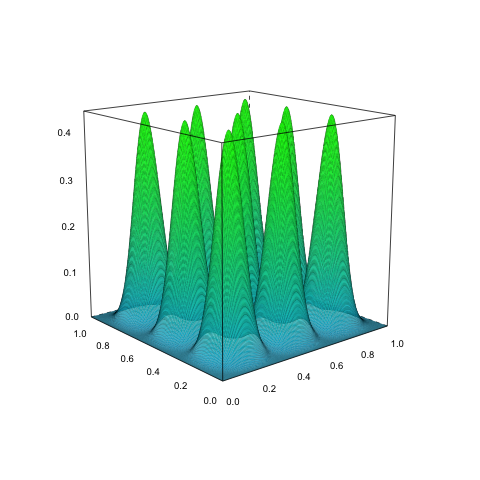
\includegraphics[width=4cm]{sparse_bicubic_basis}
% \caption{A ``thinned'' tensor product basis}
% \end{figure}
%     \end{center}
%\end{column}
%\end{columns}
%\vspace{0.3cm}
%\begin{equation*}
%\phi\left(l,m\right) = \sum_{i=1}^K \sum_{j=1}^L \theta_{ij} B_{i}\left(l\right) B_{j}\left(m\right)
%\end{equation*}
%
 
%The parameters of the functional autoregressive model given by \ref{eq:MyModel} define the elements of the precision matrix $\Omega$, rather than the elements of $\Sigma$ itself. It is well known that if we let $Y = \left(Y_1, \dots, Y_m\right)^\prime$ denote the random vector having joint distribution with mean zero and covariance matrix $\Sigma$, then the elements of $\Sigma^{-1}=\Omega$, $\left\{ \omega_{ij} \right\}$ may be interpreted as partial covariances between the elements of $Y$. This suggests shrinking $\phi$ to zero for large values of $l$. One can show that if $T$ has $k$ non-zero diagonals, then the middle $k$ diagonals of $\Sigma^{-1}$ are non-zero.  

%For ease of exposition, we first focus our attention on the estimation of $\phi$ assume that $\sigma^2\left(t\right)$ is fixed and known. Estimation of the innovation variance function is presented in Section~\ref{section:variance-estimation}. In the case that subjects share a common set of observation times $t_1 < \dots < t_m$,  it is well known that the MLE for $\Sigma$, $S = \sum_{i=1}^N y_i y_i^\prime$ is highly unstable in high dimensions, a condition that is potentially worsened when one or more subjects has at least one observation time that is unique from the set of observation times common across subjects. To mitigate instability due to high dimensionality and simultaneously permit the estimation of $\phi\left(\cdot,\cdot\right)$ as a smooth bivariate function, we obtain a covariance estimator by applying bivariate smoothing of the elements of the Cholesky factor. 

%%====================================================================================

\section{Smoothing parameter selection}

%\subfile{chapter-3-subfiles/chapter-3-tensor-product-pspline-model-selection}
\subsubsection{The limiting behaviour of $H_\lambda$}

As with the RKHS framework and accompanying smoothing spline representation, the smoothing matrix  

\begin{equation}\label{eq:pspline-smoothing-matrix}
A_\lambda = X \big( \left(X B\right)' D^{-1} XB +  \lambda_l P_l+ \lambda_m P_m \big)^{-1}\left(X B\right)' D^{-1}
\end{equation}

\noindent
and its properties play an integral role in selecting the optimal smoothing parameter in any regularized regression, including the P-spline framework. We discussed the leave-one-subject-out cross validation score \eqref{eq:LOSOCV} and its computationally efficient approximation \eqref{eq:approx-losocv} in Chapter~\ref{SSANOVA-chapter}, which rely directly on the smoothing matrix for calculation. The results in \cite{xu2012asymptotic} are basis agnostic, so we can employ the losoCV criterion for selecting P-spline smoothing parameters as in the smoothing spline setting by replacing $\tildeA_{\lambda,\bftheta}$ with $A_\lambda$. 

\bigskip

%Summarizing the complexity of a fitted P-spline is non-trivial; it requires the simultaneous consideration of the smoothing parameters, the number of basis functions in the B-spline basis, and the order of the difference penalties. To assess model complexity, \cite{eilers1996flexible} follow \cite{hastie1990generalized}, who use the trace of the smoothing matrix as an approximation of the \textit{effective dimension} (ED) of a linear smoother. The effective (model) dimension is defined as 
%
%%\begin{align}
%\begin{equation} \label{eq:trace-of-the-smoothing-matrix}
%\textup{ED} = \textup{tr}\left( A_\lambda \right) = \textup{tr}\bigg( X\left( \left(XB\right)^\prime D^{-1}XB +  \lambda_l P_l+ \lambda_m P_m\right)^{-1} \left(X B\right)^\prime D^{-1}  \bigg)
%\end{equation}
%%\end{align}
%
%\noindent
%The ED combines the effect of the smoothing parameter, the number of basis functions, and the differencing order, and it is easy to compute. When the number of basis functions is significantly smaller than the sample size, it is advantageous to use the cyclic property of the trace: 
%
%\begin{align*}
%\textup{tr}\left( A_\lambda \right) &= \textup{tr}\bigg( X\left( \left(XB\right)^\prime D^{-1}XB +  \lambda_l P_l+ \lambda_m P_m\right)^{-1} \left(X B\right)^\prime D^{-1}  \bigg)\\
%&= \textup{tr}\bigg( \left(X B\right)^\prime D^{-1}  X\left( \left(XB\right)^\prime D^{-1}XB +  \lambda_l P_l+ \lambda_m P_m\right)^{-1} \bigg),
%\end{align*}
%
%\noindent
%which requires computing the trace of a $k_1k_2 \times k_1k_2$ matrix, which is computationally more economical when the total number of basis functions is smaller than the total number of observations. This approach to approximating the effective model dimension is also consistent with \cite{ye1998measuring}, who constructed a generalization of the concept of a model's degrees of freedom using the idea that the degrees of freedom can also be interpreted as the sum of the sensitivity of each fitted value with respect to the corresponding observed value.
%
%\bigskip
%
%Using the eigenstructure of the smoothing matrix, one can show that as the smoothing parameters tend to infinity, the effective dimension approaches $d_l + d_m$, the sum of the order of the differencing operators for $l$ and $m$. Let
%
%\begin{equation*}
%Q = \left(X B\right)^\prime D^{-1} XB \qquad \mbox{and} \qquad Q_\lambda = \lambda_l P_l + \lambda_m P_m.
%\end{equation*}
%
%Again using cyclic property of the trace, we can write
%\begin{align*}
%%\begin{split}
%\mbox{tr}\left(A_\lambda \right) &= \mbox{tr}\bigg[ \left(Q + Q_\lambda \right)^{-1}Q \bigg]\\
%&=\mbox{tr}\bigg[ Q^{1/2}\left(Q + Q_\lambda \right)^{-1}Q^{1/2} \bigg] \\
%&=\mbox{tr}\bigg[\left(I + Q^{-{1/2}}Q_\lambda Q^{-{1/2}} \right)^{-1} \bigg]
%%\end{split}
%\end{align*}
%
%\noindent
%Finally we have that
%\begin{equation*}
%\mbox{tr}\left(A_\lambda \right) = \mbox{tr}\bigg[\left(I + \lambda Q^{-{1/2}}Q_\lambda Q^{-{1/2}}  \right)^{-1} \bigg] = \sum_{j=1}^{k_1k_2} \frac{1}{1 + \lambda \gamma_j},
%\end{equation*}
%
%\noindent
%where $\gamma_j$, $j=1,\dots,k_1k_2$ are the eigenvalues of $Q^{-{1/2}}Q_\lambda Q^{-{1/2}}$. The matrix constructed from the sum of the penalty terms, $Q_\lambda$, has exactly $d_l + d_m$ eigenvalues equal to zero. Hence, $Q^{-{1/2}}Q_\lambda Q^{-{1/2}} $ has $d_l + d_m$ eigenvalues equal to zero, so for large $\lambda$, only the $d_l + d_m$ terms with $\gamma_j=0$ contribute to the sum which gives the trace of $A_\lambda$. Then
% 
% \[
%\lim_{\lambda \rightarrow \infty  } \mbox{tr}\left(A_\lambda\right) = d_l + d_m.
% \]
%
%%A further simplification of \ref{eq:hat-matrix-trace}
%%
%%\begin{align*} 
%%\left(B^T B + \lambda D^T D \right)^{-1} B^T B &= \left(B^T B + \lambda D^T D \right)^{-1} \left( B^T B + \lambda D^T D - \lambda D^T D\right) \nonumber \\
%%&= I - \lambda\left(B^T B + \lambda D^T D \right)^{-1} D^T D \label{eq:cyclic_hat_matrix_simplification}
%%\end{align*}
%%
%%\begin{align*} 
%%\left[\left(WB\right)^\prime D^{-1}WB +  \lambda_l P_l+ \lambda_m P_m\right]^{-1} \left(W B \right)^\prime D^{-1} WB  &= \left[\left(WB\right)^\prime D^{-1}WB +  \lambda_l P_l+ \lambda_m P_m\right]^{-1}\left(W B \right)^\prime D^{-1} \times \\
%%&\mbox{\;\;\;\;\;\;\;\;\;\;\;\;\;\;\;\;\;\;\;\;\;} \left[WB + \lambda_l P_l+ \lambda_m P_m - \left(\lambda_l P_l+ \lambda_m P_m\right) \right] \\
%%&= I - \lambda\left(B^T B + \lambda D^T D \right)^{-1} D^T D \label{eq:cyclic_hat_matrix_simplification}
%%\end{align*}
%
%This clearly shows that the effective dimension is always less than $k_1k_2$, the number of B-spline used in the regression basis; further, the effective dimension is always smaller than $\min\left(\sum_{i=1}^N p_i - N, k_1k_2\right)$. This is visually demonstrated in Figure~\ref{fig:pspline-limiting-effective-dimension}, which displays impact of the smoothing parameter on the effective dimension of the P-spline fit to the simulated data shown in Figure~\ref{fig:overcomplete-pspline-basis}. As $\lambda$ increases, the effective dimension approaches the order of the difference penalty. Even for small $\lambda$, the effective dimension never exceeds the number of observations, so there are no issues when fitting P-splines with many more basis functions than observations. 
%
%\begin{figure}[H]
%\begin{center}
%\graphicspath{{img/}}
% 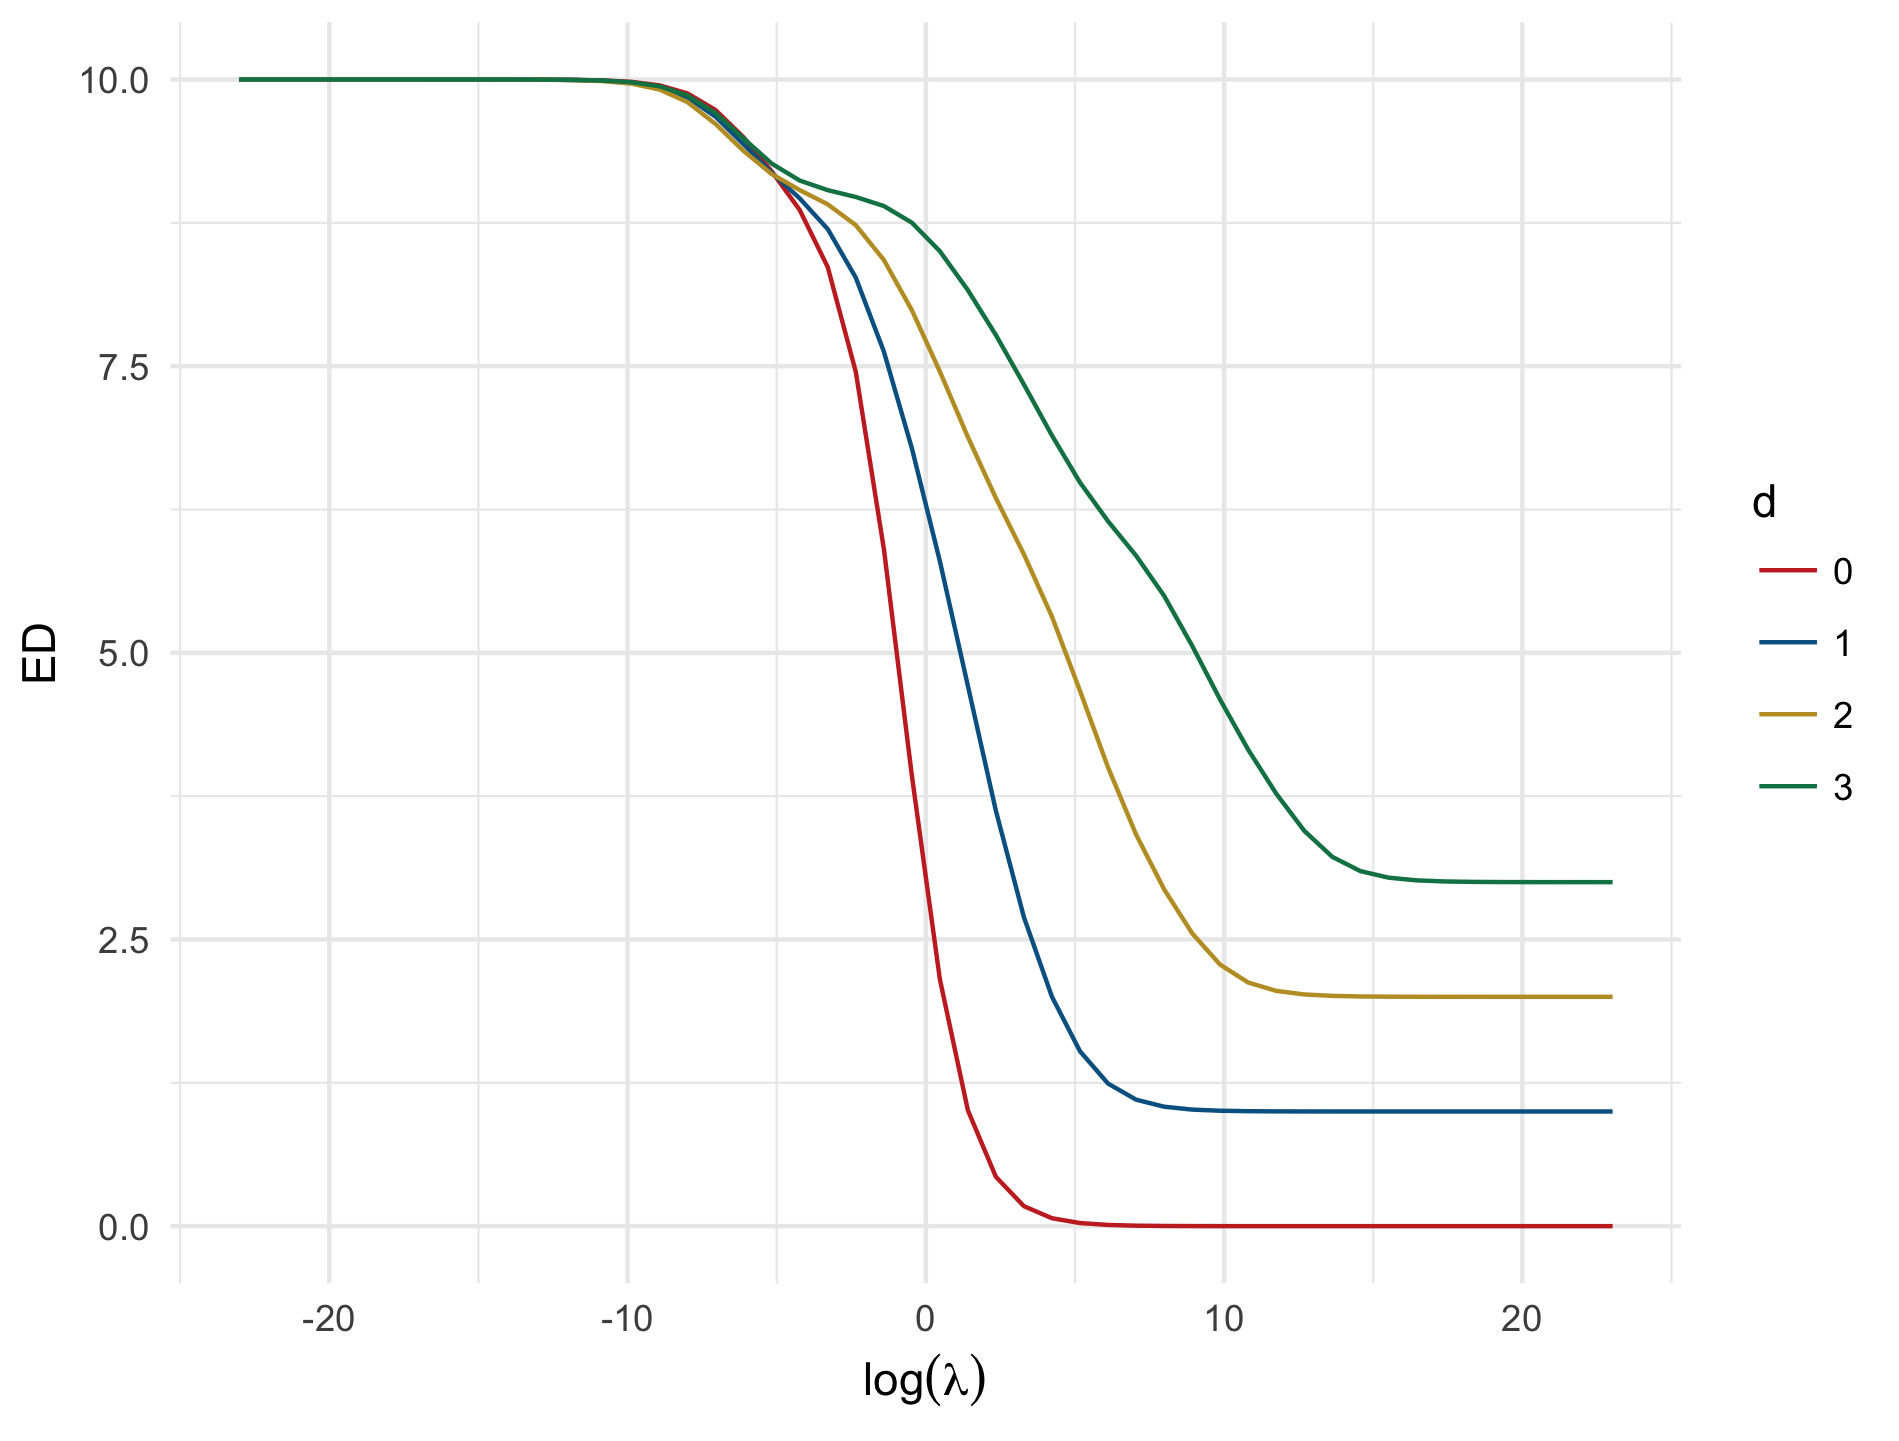
\includegraphics[width=0.7\textwidth]{pspline-limiting-effective-dimension}
%\caption{\textit{The limiting behaviour of the trace of the smoothing matrix $A_\lambda$ as the smoothing parameter increases for the P-spline fit to the 10 observations using 60 B-spline basis functions, shown in Figure~\ref{fig:overcomplete-pspline-basis}. For weakly enforced smoothing, the effective dimension is equal to the number of observations, and as $\lambda \rightarrow \infty$, the effective dimension approaches the order of the difference penalty.}} \label{fig:pspline-limiting-effective-dimension}
%\end{center}
%\end{figure}

The effective model dimension is closely connected to model selection criteria; \cite{eilers1996flexible} propose the use of the Akaike information criterion (AIC) for selecting the optimal value of the smoothing parameters $\lambda = \left(\lambda_l, \lambda_m\right)$, which is equivalent to the unbiased risk estimator discussed in Chapter~\ref{SSANOVA-chapter} under a Gaussian likelihood. For a detailed discussion of the connection between the unbiased risk estimate and AIC in the non-gaussian case, see \cite{wood2017generalized}, Chapter 4, Section 5. The same reference provides a detailed discussion of computational methods for minimizing the unbiased risk estimate with respect to multiple smoothing parameters. The algorithm shares the same basic structure as the one outlined in Section~\ref{gaussian-unbiased-risk-estimate}, with modifications on the derivatives and the Hessians to account for the fact that the P-spline basis and penalty are constructed independently of one another.



\section{The P-spline estimator for the innovation variance function}

The P-spline estimator for the log innovation variance function is constructed via penalized similarly to the smoothing spline estimator in Section~\ref{chapter-3-IV-modeling-section}.  As before, given an estimate $\phi^*$ of $\phi$, fixing $\phi = \phi^*$, the the log likelihood of the squared working residuals is given by 

\begin{equation} \label{eq:penalized-joint-loglik-given-phi-3}
-\ell\left( \sigma^2  \vert Z_1,\dots, Z_N, \phi,  \right) =  \sum_{i = 1}^N \sum_{j = 1}^{p_i} \log \sigma^2_{ij}  + \sum_{i = 1}^N \sum_{j = 1}^{p_i} \frac {z_{ij}}{\sigma^2_{ij}},
\end{equation}
\noindent

where $\epsilon_{ij} =  y_{ij} - \sum\limits_{k<j} \phi^*_{ijk} y_{ik}$, and $z_{ij} = \epsilon_{ij}^2$. We can approximate $\eta \left(t\right) = \log \sigma^2\left(t\right)$ using a B-spline basis expansion, modeling
\[
\eta\left(t\right) = \sum\limits_{j = 1}^K \theta_j B_{j}\left(t\right).
\] 
\noindent
Model estimation and smoothing parameter selection can be carried out using performance-oriented iteration as described in Section~\ref{smoothing-parameter-selection-exponential-families}, substituting the above expansion for $\eta$ and trading the smoothing spline penalty for the discrete difference penalty \eqref{eq:bspline-difference-penalty-1}. For detailed presentation of optimization procedures, see \cite{marx1999generalized}. 

   
\chapter{Simulation studies} \label{simulation-studies-chapter}


In this section we compare bivariate spline estimators of the Cholesky factor to other methods of covariance estimation. Our primary comparisons are that with the parametric polynomial estimator proposed by \cite{pourahmadi1999joint},  \cite{pan2003modelling}, and \cite{pourahmadi2002dynamic}, which is also based on the modified Cholesky decomposition, and with the oracle estimator, which effectively gives a lower bound on the risk for given covariance structure. As a benchmark, we also include the sample covariance matrix, and two regularized variants of it: the tapered sample covariance matrix \citep{cai2010optimal} and the soft thresholding estimator \citep{rothman2009generalized}, which does not rely on a natural ordering among the variables. In the simulations, the smoothing spline estimator of the modified Cholesky decomposition was constructed using the framework of a tensor product cubic smoothing spline. For each covariance matrix used for simulation, the P-spline estimator was constructed so that the order of the difference penalties for $l$ and $m$ are treated as additional tuning parameters.

\bigskip

Simulations were carried out for five covariance structures: the diagonal covariance with homogenous variances, a heterogenous autoregressive process with linear varying coefficient function, the same heterogeneous process but truncated to zero to band the inverse covariance matrix, the rational quadratic covariance model, and the compound symmetric model. The two-dimensional surfaces corresponding to each of these are shown left to right in Figure~\ref{fig:true-covariance-heatmaps}. The first row of image plots display the surface which coincides with the appropriate discrete covariance matrix, and in the second row are the surface maps of the corresponding Cholesky factors. Precise models used for simulations are defined in Table~\ref{table:simulation-model-list}. 

\begin{table}[H]
\centering
\caption{\textit{Covariance models used for data generation in the simulation study.}}
\begin{tabular}{p{7cm}p{7cm}}
\hline
 \multicolumn{2} {l} {I: Mutual independence} \\[0.3cm]
 $\Sigma = \mathrm{I}$ & $\begin{aligned}
\phi\left(t,s\right) &= 0, \quad 0 \le s < t \le 1,\\[0.15cm] 
\sigma^2\left(t\right) &= 1, \quad 0 \le t \le 1.
\end{aligned}$ \\[0.2cm]
\\
\hline
\\
 \multicolumn{2} {l} {II: Linear varying coefficient function, constant innovation variances} \\[0.3cm]
$\Sigma = T^{-1} D {T'}^{-1}$ & $\begin{aligned}
\phi\left(t,s\right) &= t - \frac{1}{2},  \quad 0 \le t \le 1, \\[0.15cm]
\sigma^2\left(t\right) &= 0.1^2,  \quad 0 \le t \le 1.
\end{aligned}$ \\
\\
\hline
\\
\multicolumn{2} {l} {III: Banded linear varying coefficient function, constant innovation variances} \\[0.3cm]
 $\Sigma = T^{-1} D {T'}^{-1}$ &$ \begin{aligned}
\phi\left(t,s\right) &= \left\{\begin{array}{ll} t - \frac{1}{2}, & t - s \le 0.5\\ 
0, & t - s > 0.5\end{array}\right.,\\[0.15cm]
\sigma^2\left(t\right) &= 0.1^2, \quad 0 \le t \le 1.
\end{aligned}$  \\
\\
\hline
\\
\multicolumn{2} {l} {IV: Rational quadratic covariance} \\[0.3cm]
 $\Sigma = \left[\sigma_{ij}\right]$ &  $\begin{aligned}\sigma_{ij} &=\begin{array}{ll} \left(1 + \frac{\left(t_i - t_j\right)^2}{2\alpha k^2}\right)^{-\alpha}, & 0 < t_i, t_j < 1\end{array}\\
                                                                      k &= 0.6,\;\;\alpha = 1\end{aligned}$ \\
 \\
\hline
\\
\multicolumn{2} {l} {V: Compound symmetry} \\[0.3cm]
 $\begin{array}{l}\Sigma = \sigma^2\left(\rho \mathrm{J} + \left(1-\rho\right)\mathrm{I}\right),  \\
 \\
  \rho=0.7, \quad \sigma^2=1 \end{array}$  &  $\begin{aligned}
\phi_{ts} &= \frac{\rho}{1 + \left(t-2\right)\rho}, \begin{array}{l} t = 2, \dots, M,\\ 
				 s = 1, \dots, t-1 \end{array}\\
\sigma_t^2 &= \left\{\begin{array}{ll} 1, & t = 1\\ 1 -\frac{\left(t-2\right)\rho^2}{1 + \left(t-2\right)\rho}, & t = 2, \dots, M \end{array}\right.
\end{aligned}$ \\
 \\
\hline
\end{tabular} \label{table:simulation-model-list}
\end{table}


\bigskip

Figure~\ref{fig:true-covariance-heatmaps} displays a two dimensional representation of each covariance matrix $\Sigma$ and it's corresponding Cholesky factor $T$ used in the simulation study. The smallest elements of each matrix correspond to dark green pixels, while the light pink (white) pixels correspond to the large (largest) elements of the matrix. Comparison of the covariance matrices with the generalized autoregressive coefficient function which defines lower triangular surface in the second row demonstrates that covariance structures exhibiting sparsity or parsimony do not necessarily exhibit the same simplicity in the components of the Cholesky decomposition. The Cholesky factor for Model III, the truncated linear varying coefficient AR model, is sparse, with elements on the outer half of the subdiagonals equal to zero. While this corresponds to a banded inverse covariance structure, $\Sigma$ itself is not sparse.  The compound symmetric model has simple structure and is parsimonious; its dependence parameters can be expressed as the evaluation of a function which is constant in time $t$. However, the elements of the Cholesky factor and diagonal matrix of innovation variances $D = T \Sigma T'$ do not exhibit such elementary structure, the elements of which are nonlinear in $t$. 

%\subfile{chapter-4-subfiles/chapter-4-true-covariance-heatmaps}
\begin{figure}[H] 
\begin{center}
  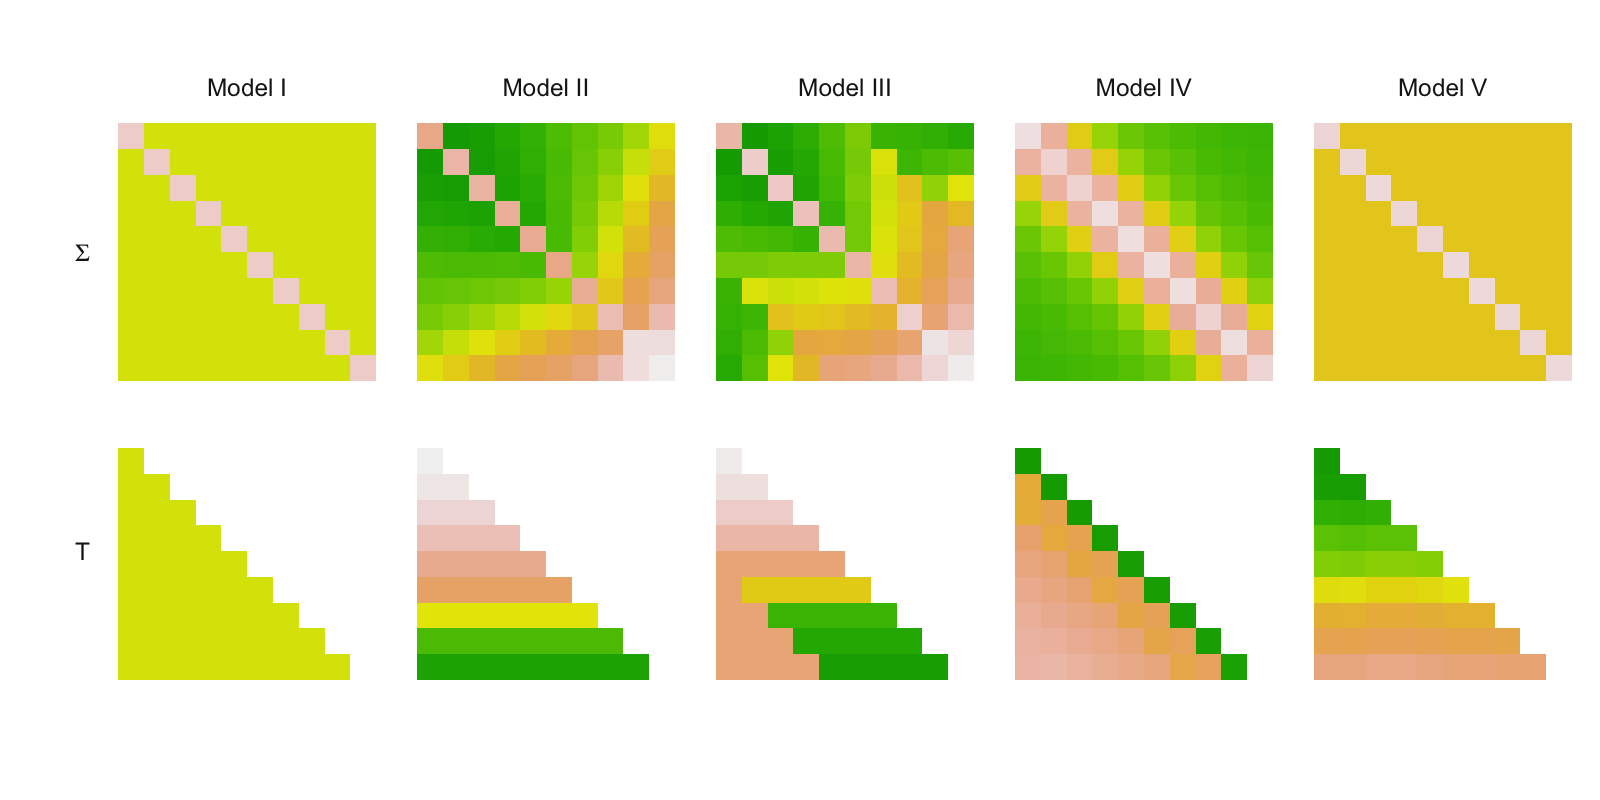
\includegraphics[width = \textwidth]{img/chapter-4/cov-cholesky-grid}%}
\caption{\textit{Heatmaps of the true covariance matrices (row 1) under simulation Model I - Model V (see Table~\ref{table:simulation-model-list}) and the function $\phi$ defining the corresponding Cholesky factor $T$ (row 2).} } \label{fig:true-covariance-heatmaps}
\end{center}
\end{figure}


\bigskip

%\subfile{chapter-4-subfiles/chapter-4-true-covariance-functions}

%%%%%%%%%%%%%%%%%%%%%%%%%%%%%%%%%%%%%%%%%%%%%%%%%%%%%%%%%%%%%%%%%%%%%%%%%%%%%%%%%%%%%%%%%%%%%%%%
%%%%%%%%%%%%%%%%%%%%%%%%%%%%%%%%%%%%%%%%%%%%%%%%%%%%%%%%%%%%%%%%%%%%%%%%%%%%%%%%%%%%%%%%%%%%%%%%
%%%%%%%%%%%%%%%%%%%%%%%%%%%%%%%%%%%%%%%%%%%%%%%%%%%%%%%%%%%%%%%%%%%%%%%%%%%%%%%%%%%%%%%%%%%%%%%%
%%%%%%%%%%%%%%%%%%%%%%%%%%%%%%%%%%%%%%%%%%%%%%%%%%%%%%%%%%%%%%%%%%%%%%%%%%%%%%%%%%%%%%%%%%%%%%%%
%%%%%%%%%%%%%%%%%%%%%%%%%%%%%%%%%%%%%%%%%%%%%%%%%%%%%%%%%%%%%%%%%%%%%%%%%%%%%%%%%%%%%%%%%%%%%%%%

\section{Loss Functions and Risk Measures}
Let $\hat{\Sigma}$ be an estimator of the true $M \times M$ covariance matrix $\Sigma$. To assess performance of an estimator $\hat{\Sigma}$, we consider two commonly loss functions:
\begin{equation} \label{eq:quad-loss}
\Delta_1\left(\Sigma,\hat{\Sigma} \right) = tr\left(\left( \Sigma^{-1} \hat{\Sigma} - \mathrm{I}\right)^2 \right),
\end{equation}
\noindent
\begin{equation} \label{eq:entropy-loss}
\Delta_2\left(\Sigma,\hat{\Sigma}\right) = tr\left( \Sigma^{-1} \hat{\Sigma} \right) - log \vert \Sigma^{-1} \hat{\Sigma} \vert - M.
\end{equation}
\noindent
$\Sigma$ denotes the true covariance matrix and $\hat{\Sigma}$ is an $M \times M$ positive definite matrix. Each of these loss functions is $0$ when $\hat{\Sigma} = \Sigma$ and is positive when $\hat{\Sigma} \ne \Sigma$. Both measures of loss are scale invariant. If we let random vector $Y$ have covariance matrix $\Sigma$, and define the $Z$ as some linear transformation of $Y$:

\[
Z = CY. 
\]
\noindent
for some $M \times M$ matrix $C$,  then $Z$ has covariance matrix $\Sigma_Z = C \Sigma C'$. Given an estimator $\hat{\Sigma}$ of $\Sigma$, one immediately obtains an estimator for $\Sigma_Z$, $\hat{\Sigma}_Z = C \hat{\Sigma} C'$. If $C$ is invertible, then the loss functions $\Delta_1$ and $\Delta_2$ satisfy
\[
\Delta_i\left(\Sigma,\hat{\Sigma}\right) = \Delta_i\left(C \Sigma C', C \hat{\Sigma}C' \right). 
\]
\noindent
The first loss $\Delta_1$, or the quadratic loss, measures the discrepancy between $\left(\Sigma^{-1} \hat{\Sigma}\right)$ and the identity matrix with the squared Frobenius norm. The Frobenius norm of a matrix $A$ is given by 

\[
\vert \vert A \vert \vert_F^2 = \mbox{tr}\left(A A'\right).
\]
\noindent
The second loss $\Delta_2$ is commonly referred to as the entropy loss; it gives the Kullback-Leibler divergence of two multivariate Normal densities with the same mean and the two corresponding covariance matrices. The quadratic loss penalizes overestimates more than underestimates, so ``smaller'' estimates are favored more under $\Delta_1$ than $\Delta_2$. For example, among the class of estimators comprised of scalar multiples $cS$ of the sample covariance matrix, \cite{haff1980empirical} established that $S$ is optimal under $\Delta_2$, while the smaller estimator $\frac{NS}{N+M+1}$ is optimal under $\Delta_1$. 

\bigskip

Given $\Sigma$, the corresponding values of the risk functions are obtained by taking expectations:

\begin{equation*}
R_i \left(\Sigma,\hat{\Sigma}\right) = E_\Sigma\left[\Delta_i\left(\Sigma,\hat{\Sigma}\right)\right], \quad i = 1,2.
\end{equation*}
\noindent
We prefer an estimator $\hat{\Sigma}$ with smaller risk.  Given $\Sigma$, we can estimate the risk of an estimator via Monte Carlo approximation. 

%%%%%%%%%%%%%%%%%%%%%%%%%%%%%%%%%%%%%%%%%%%%%%%%%%%%%%%%%%%%%%%%%%%%%%%%%%%%%%%%%%%%%%%%%%%%%%%%
%%%%%%%%%%%%%%%%%%%%%%%%%%%%%%%%%%%%%%%%%%%%%%%%%%%%%%%%%%%%%%%%%%%%%%%%%%%%%%%%%%%%%%%%%%%%%%%%
%%%%%%%%%%%%%%%%%%%%%%%%%%%%%%%%%%%%%%%%%%%%%%%%%%%%%%%%%%%%%%%%%%%%%%%%%%%%%%%%%%%%%%%%%%%%%%%%
%%%%%%%%%%%%%%%%%%%%%%%%%%%%%%%%%%%%%%%%%%%%%%%%%%%%%%%%%%%%%%%%%%%%%%%%%%%%%%%%%%%%%%%%%%%%%%%%
%%%%%%%%%%%%%%%%%%%%%%%%%%%%%%%%%%%%%%%%%%%%%%%%%%%%%%%%%%%%%%%%%%%%%%%%%%%%%%%%%%%%%%%%%%%%%%%%

\section{Alternative Estimators}
%\subfile{chapter-4-subfiles/chapter-4-benchmark-estimators}
The following estimators serve as benchmarks for performance under the five simulation settings outlined above: the MCD polynomial estimator $\hat{\Sigma}_{poly}$, the sample covariance matrix $S$, the soft thresholding estimator $S^\lambda$, and the tapering estimator $S^\omega$. We will review the general definitions of these, but for detailed discussion of the construction and properties of these estimators, see Sections~\ref{elementwise-shrinkage-estimators} and \ref{chapter-1-matrix-decompositions}.

\bigskip

In the spirit of the GLM, the MCD polynomial estimator is a particular case of estimators which model the components of the Cholesky decomposition using covariates. The polynomial estimator takes the GARPs and IVs to be polynomials of lag and time, respectively:

\begin{align*}
\begin{split}  \label{eq:GARP-IV-parametric-model}
\phi_{jk} &= z'_{jk} \gamma \\
\log \sigma^2_{j} &= z'_{j}\lambda, 
\end{split}
\end{align*}
\noindent
for $j = 1,\dots, M$, $k = 1,\dots, j-1$. The vectors $z_j$ and $z_{jk}$ are of dimension $q \times 1$ and $p \times 1$  which hold covariates

\begin{align}
\begin{split} 
z'_{jk} &= \left(1, t_j - t_k, \left(t_j - t_k\right)^2,\dots, \left(t_j - t_k\right)^{p-1}\right)', \\
z'_{j}  &= \left(1, t_j, \dots, t_j^{q-1}\right)'.
\end{split}
\end{align} \label{eq:mcd-polynomial-model}
\noindent
where the orders of the polynomials, $p$ and $q$, are chosen by BIC. 

\bigskip

\cite{rothman2009generalized} presented a class of generalized thresholding estimators, including the soft-thresholding estimator given by

\[
S^{\lambda}=   \begin{bmatrix} \mbox{sign}\left(s_{ij}\right) \left(s_{ij} - \lambda\right)_+ \end{bmatrix},
\]
\noindent 
where $\sigma^*_{ij}$ denotes the $i$-$j^{th}$ entry of the sample covariance matrix, and $\lambda$ is a penalty parameter controlling the amount of shrinkage applied to the empirical estimator. 

\bigskip

The tapering estimator proposed by \cite{cai2010optimal} is given by
\[
S^{\omega} =  \begin{bmatrix} \omega_{ij}^k s_{ij} \end{bmatrix},
\]
\noindent
where the $\omega_{ij}^k$ are given by 
\begin{equation*}
\omega^k_{ij} = k_h^{-1} \left[ \left( k - \vert i-j\vert\right)_+ - \left(k_h - \vert i-j\vert\right)_+ \right],
\end{equation*}
\noindent
The weights $\omega^k_{ij}$ are controlled by a tuning parameter, $k$,  which can take integer values between 0 and $M$. Without loss of generality,  we assume that $k_h = k/2$ is even. The weights may be rewritten as
\begin{align*}
\omega_{ij} = \left\{\begin{array}{ll} 1, & \vert i -j \vert \le k_h \\
                             2 - \frac{i - j}{k_h}, & k_h < \vert  i -j \vert \le k, \\
                             0, & \mbox{otherwise}  \end{array} \right.
\end{align*}
\noindent

\bigskip

Tuning parameter selection for the regularized versions of the sample covariance matrix was performed using cross validation. Under certain conditions pertaining to the ratio of sample sizes of the training and validation datasets, the $K$-fold cross validation criterion is a consistent estimator of the Frobenius norm risk. It is defined 

\begin{equation} \label{eq:K-fold-matrix--cv}
\mbox{CV}_F\left(\lambda \right) = \argmin{\lambda} K^{-1} \sum_{k = 1}^K  \vert \vert\hat{\Sigma}^{\left(-k\right)} - \tilde{\Sigma}^{\left(k\right)}  \vert \vert_F^2, 
\end{equation}
\noindent
There is little established about the optimal method for tuning parameter selection in for the class of estimators based on element-wise shrinkage of the sample covariance matrix.  However, based on the results of an extensive simulation study presented in \cite{fang2016tuning}, we use $K = 10$-fold cross validation to select the tuning parameters for both the tapering estimator $S^\omega$ and the soft thresholding estimator $S^{\lambda}$. They authors implement cross validation for a number of element-wise shrinkage estimators for covariance matrices in the \cite{CVTuningCov} R package, which was used to calculate the risk estimates for $S^{\omega}$ and $S^{\lambda}$. 

\bigskip

As discussed in Chapter 1, in the limit, soft thresholding produces a positive definite estimator with probability tending to 1 (\cite{rothman2009generalized}), however element-wise shrinkage estimators of the covariance matrix, including the soft thresholding estimator, are not guaranteed to be positive definite. We observed simulations runs which yielded a soft thresholding estimator that was indeed not positive definite.  In this case, the estimate has at least one eigenvalue less than or equal to zero, and the evaluation of the entropy loss \ref{eq:entropy-loss} is undefined. To enable the evaluation of the entropy loss, we coerced these estimates to the ``nearest'' positive definite estimate via application of the technique presented in \cite{cheng1998modified}.  For a symmetric matrix $A$, which is not positive definite,  a modified Cholesky algorithm produces a symmetric perturbation matrix $E$ such that $A + E$ is positive definite.

\bigskip

\cite{pan2003modelling} present an iterative procedure for estimating coefficient vectors $\lambda$, $\gamma$ of the polynomial model \ref{eq:mcd-polynomial-model}. Their algorithm uses a quasi-Newton step for computing the MLE under the multivariate normal likelihood. Their work is  is implemented in the JMCM package for \textsf{R}, which we used to compute the polynomial MCD estimates.  For implementation details, see \cite{pan2017jmcm}. 	 

\bigskip

In addition to these estimators, we include risk estimates for the oracle estimator for each of the simulation models in Table~\ref{table:simulation-model-list}, which serves as a practical lower bound for the risk under each generating model. For the case of mutual independence with constant variance, the oracle estimator of the covariance matrix is a diagonal matrix with the diagonal elements given by $\hat{\sigma^2}$, which is an estimate of the variance based on all of the data, $y_{ij}$, $i = 1,\dots, N$, $j = 1,\dots, m_i$. The oracle estimator for Model II is obtained by fitting the model

\begin{equation} \label{eq:model-2-oracle-model}
y\left(t_{ij}\right) = \sum_{k < j} \left(\beta_0 + \beta_1 t_{ij}\right) y\left( t_{ik} \right) + \epsilon_{ij},
\end{equation}
\noindent 
where $\epsilon_{ij}$ are independent mean zero Normal random variables with common variance $\sigma^2$. The estimator of $\bfbeta = \left(\beta_0, \beta_1\right)'$, $\hat{\bfbeta}$ is taken to be 

\begin{equation}\label{eq:model-2-oracle-estimator}
\argmin{\beta} \vert \vert Y - X B \beta \vert \vert^2, 
\end{equation}
\noindent
where $X$ denotes the matrix of autoregressive covariates as defined in (\ref{eq:ar-design-matrix-1}) and Example~\ref{example:construction-of-X}, and the matrix $B$ contains the basis for a linear function of $t$:

\[
\begin{bmatrix}
1 & t_{11} \\
1 & t_{12} \\
\vdots & \vdots \\
1 & t_{1,m_1} \\
\vdots & \vdots \\
1 & t_{N,1} \\
\vdots & \vdots \\
1 & t_{N,m_N} \\
\end{bmatrix}.
\]
\noindent
The estimator for $\sigma^2\left(t\right)$ is then the mean of the squared residuals:

\[
\hat{\sigma^2\left( t \right)} = \frac{1}{N}\sum_{i = 1}^N\frac{1}{m_i - 1} \sum_{j = 1}^{m_i} e_{ij}^2,
\]
\noindent
where $e_{i1} = y_{i1}$, $i = 1,\dots, N$. The oracle estimator for Model III is obtained in the same fashion, but $y\left(t_{ij}\right)$ is regressed only on its predecessors such that $t_{ij} - t_{ik} < 0.5$:

\begin{equation} \label{eq:model-3-oracle-model}
y\left(t_j\right) = \sum_{ t_j - t_k < 0.5} \left(\beta_0 + \beta_1 t_j\right) y\left( t_k \right) + \epsilon. 
\end{equation}

The oracle estimator under Model IV, the rational quadratic covariance model, assumes that $Y_1, \dots, Y_N$ is a random sample from a mean zero multivariate normal distribution with covariance matrix $\Sigma = \begin{bmatrix} \sigma_{ij} \end{bmatrix}$, where the elements of the covariance matrix are defined according to the parametric function given in Table~\ref{table:simulation-model-list}.

\bigskip

The compound symmetric covariance model (V) can be written as a simple random effects model:

\begin{equation} \label{eq:model-5-oracle-model}
Y_i = Z_i b_i + \bfepsilon_i,
\end{equation}
\noindent
where $\bfepsilon_i$ is a vector of residuals from a $N\left(0,\sigma_\epsilon^2\right)$ distribution, and the $b_i$ are independent $N\left(0,\sigma_b^2 \mathrm{I}\right)$ random vectors, the elements of which are mutually independent of the elements of $\epsilon_{i}$. The matrix of covariates corresponding to the random effects contains only an intercept term:

\[
Z_i = \begin{bmatrix}  1 \\ 1 \\ \vdots \\1 \end{bmatrix}.
\]
\noindent
Under this model, the within-subject covariance structure is given by
\[
Cov\left(Y_i\right) = \sigma_\epsilon^2 \mathrm{I} +  \sigma_b^2 1 1'. 
\]
\noindent
The oracle estimator can be obtained using restricted maximum likelihood estimation under a Normal likelihood with this covariance structure.

%\subfile{chapter-4-subfiles/chapter-4-benchmark-study-discussion}

%%%%%%%%%%%%%%%%%%%%%%%%%%%%%%%%%%%%%%%%%%%%%%%%%%%%%%%%%%%%%%%%%%%%%%%%%%%%%%%%%%%%%%%%%%%%%%%%
%%%%%%%%%%%%%%%%%%%%%%%%%%%%%%%%%%%%%%%%%%%%%%%%%%%%%%%%%%%%%%%%%%%%%%%%%%%%%%%%%%%%%%%%%%%%%%%%
%%%%%%%%%%%%%%%%%%%%%%%%%%%%%%%%%%%%%%%%%%%%%%%%%%%%%%%%%%%%%%%%%%%%%%%%%%%%%%%%%%%%%%%%%%%%%%%%
%%%%%%%%%%%%%%%%%%%%%%%%%%%%%%%%%%%%%%%%%%%%%%%%%%%%%%%%%%%%%%%%%%%%%%%%%%%%%%%%%%%%%%%%%%%%%%%%
%%%%%%%%%%%%%%%%%%%%%%%%%%%%%%%%%%%%%%%%%%%%%%%%%%%%%%%%%%%%%%%%%%%%%%%%%%%%%%%%%%%%%%%%%%%%%%%%
\section{Data Generation Procedures}

For each of the covariance models, we generated a set of observations of sample size $N = 50, 100$ from a multivariate normal distribution for each of three different values of within-subject sample size $M = 10, 20, 30$. To generate data according to Models II and III, which are parameterized in terms of the components of the Cholesky decomposition, the Cholesky factor $T$ and diagonal innovation variance matrix $D$ are constructed by evaluating $\phi$ and $\sigma^2$ at the fixed observation times. The data are then sampled according to the multivariate normal distribution with covariance matrix $\Sigma = T^{-1} D {T'}^{-1}$. Given covariance matrix $\Sigma$, risk estimates are obtained from$N_{sim} = 100$ samples from an $M$-dimensional multivariate Normal distribution with mean zero and the same covariance.  Since construction of the sample covariance matrix $S$, $S^\omega$, and $S^\lambda$ rely on having an equal number of regularly-spaced observations on each subject, simulations comparing performance across estimators were conducted using complete data with common measurement times across all $N$ subjects. The observation times, which are equally spaced, are mapped from the integers $1,2, \dots, M$ to the unit interval for estimation.

\bigskip

Our second concern in evaluation of our methods is how performance changes when the data exhibit varying degrees of sparsity. We fix the number of sampled trajectories $N$ and vary $M$, the size of the set  of possible measurement times

\[
t_1,\dots, t_M.
\]
\noindent
We generate irregular data by first generating a complete dataset as we did for the first simulation study:

\begin{align*}
Y_1 &= \left(y_1\left(t_1\right), y_1\left(t_2\right), \dots, y_1\left(t_M\right)\right)' \\
Y_2 &= \left(y_2\left(t_1\right), y_2\left(t_2\right), \dots, y_2\left(t_M\right)\right)' \\
&\vdots \\
Y_N &= \left(y_N\left(t_1\right), y_N\left(t_2\right), \dots, y_N\left(t_M\right)\right)',
\end{align*}
\noindent
where $Y_1,\dots, Y_N$ are independently and identically distributed according to an $M$-dimensional multivariate Normal distribution with mean zero and having covariance structure identical to one of Models I - V in \ref{table:simulation-model-list}. To induce sparsity, we subsample from the complete data $\left\{y_i\left(t_j\right) \right\}$, $i = 1,\dots, N$, $j = 1,\dots, M$, randomly omitting an observation $y_i\left(t_j\right)$ with probability $0.1$, $0.2$, and $0.3$. For both sets of simulations, the smoothing parameters for the smoothing spline and P-spline estimators were selected using both leave-one-subject-out cross validation $\mbox{losoCV}\left(\lambda\right)$ and unbiased risk estimate $\mbox{U}\left(\lambda\right)$. Given the selected values of the tuning parameters, we computed the estimated covariance matrix and compared it to the true covariance matrix via entropy loss and quadratic loss. 

%%%%%%%%%%%%%%%%%%%%%%%%%%%%%%%%%%%%%%%%%%%%%%%%%%%%%%%%%%%%%%%%%%%%%%%%%%%%%%%%%%%%%%%%%%%%%%%%
%%%%%%%%%%%%%%%%%%%%%%%%%%%%%%%%%%%%%%%%%%%%%%%%%%%%%%%%%%%%%%%%%%%%%%%%%%%%%%%%%%%%%%%%%%%%%%%%
%%%%%%%%%%%%%%%%%%%%%%%%%%%%%%%%%%%%%%%%%%%%%%%%%%%%%%%%%%%%%%%%%%%%%%%%%%%%%%%%%%%%%%%%%%%%%%%%
%%%%%%%%%%%%%%%%%%%%%%%%%%%%%%%%%%%%%%%%%%%%%%%%%%%%%%%%%%%%%%%%%%%%%%%%%%%%%%%%%%%%%%%%%%%%%%%%
%%%%%%%%%%%%%%%%%%%%%%%%%%%%%%%%%%%%%%%%%%%%%%%%%%%%%%%%%%%%%%%%%%%%%%%%%%%%%%%%%%%%%%%%%%%%%%%%

\section{Results}

\subsection{Simulations with Complete Data}
Figure~\ref{fig:cov-estimate-lattice} provides a visual summary of the qualitative differences between the estimates resulting from each of the eight methods of estimation for the five covariance structures used for simulation. The first row in the grid shows the surface plot of each of the true covariance structures, and each row thereafter corresponds to the five covariance estimates for the given estimation method. The surface plots of the oracle estimate in the second row serve as a point of reference for the `gold standard` in each scenario, since the oracle estimates were constructed assuming that the functional form of the covariance is known (either the full covariance structure or the components of the Cholesky decomposition.) The corresponding estimates of the Cholesky factor $T$ for the estimators based on the modified Cholesky decomposition are shown in Figure~\ref{fig:chol-estimate-lattice}, and the decomposition of the $\hat{T}$ corresponding to the smoothing spline ANOVA estimator $\hat{\Sigma}_{SS}$ into functional components is displayed in Figure~\ref{fig:ssanova-component-lattice}

%\subfile{chapter-4-subfiles/chapter-4-cov-lattice-ggplot}

\begin{figure}[H] 
\centering
\caption{\textit{Covariance Model I - Model V (see Table~\ref{table:simulation-model-list}) used for simulation and corresponding estimates. The columns in the grid correspond to each simulation model. The first row of shows the true covariance structure, and each row beneath corresponds to each of the estimators.}}
  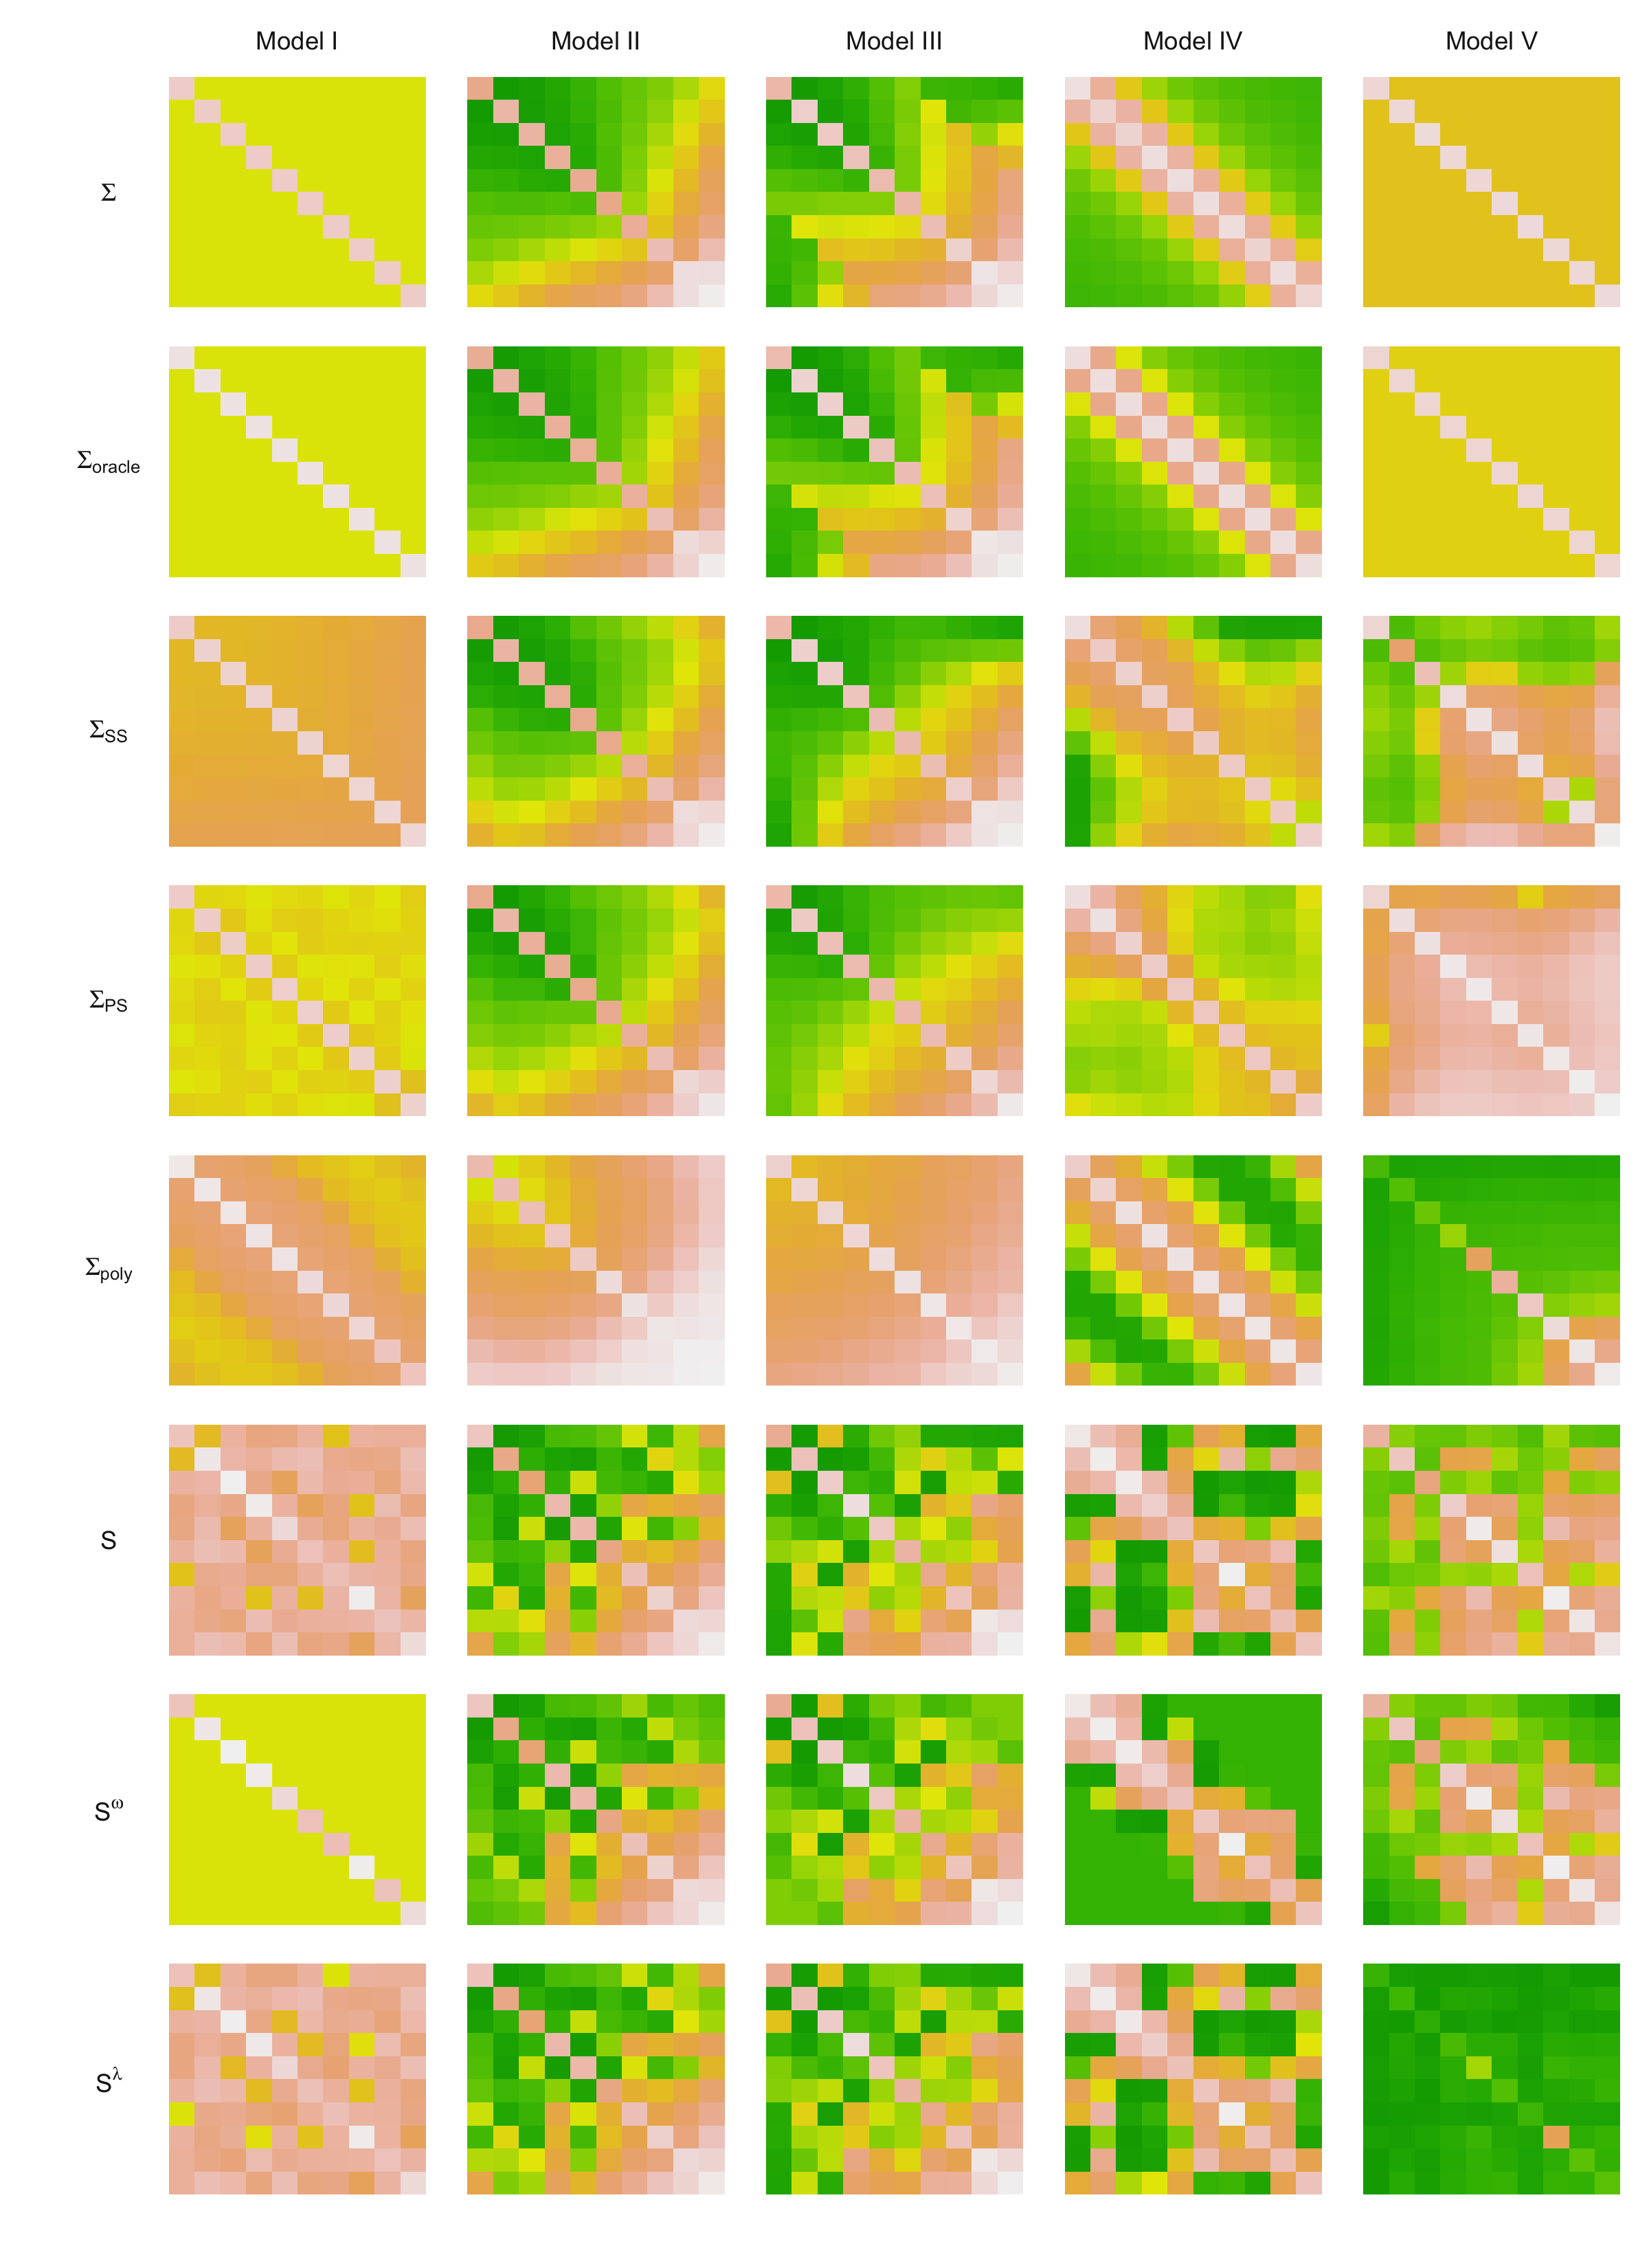
\includegraphics[width = 1\textwidth]{img/chapter-4/cov-estimate-lattice}\label{fig:cov-estimate-lattice}
\end{figure}

\begin{figure}[H] 
\centering
\caption{\textit{The generalized autoregressive coefficient function $\phi$ which defines the elements of the true lower triangle of Cholesky factor $T$ corresponding to Model I - Model V and estimates of the same surface for estimators based on the modified Cholesky decomposition. The true covariance structure is displayed across the top row.}}
  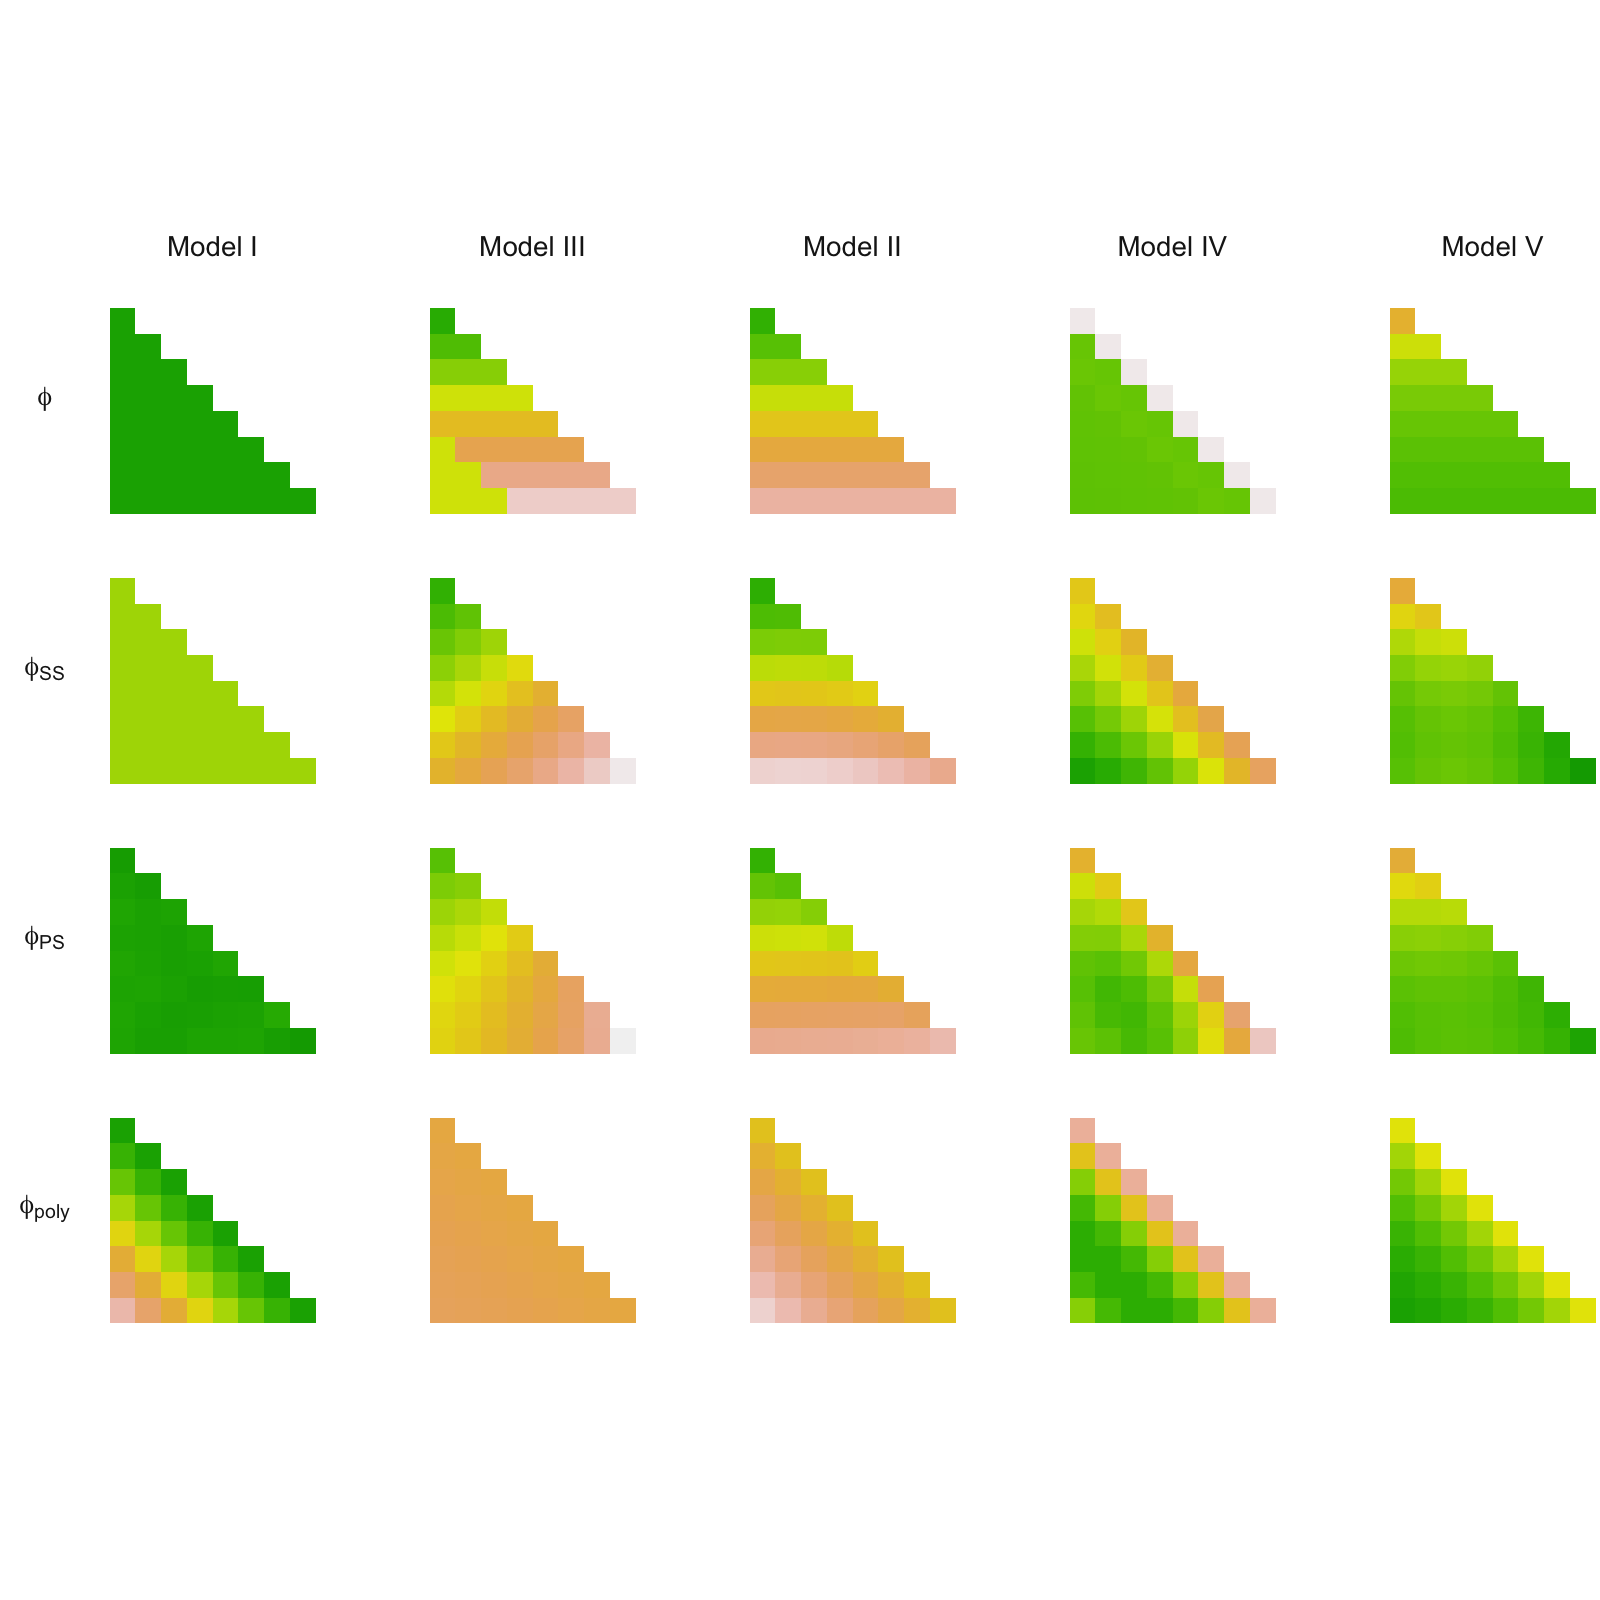
\includegraphics[width = 1\textwidth]{img/chapter-4/cholesky-estimate-lattice}
  \label{fig:chol-estimate-lattice}
\end{figure}

%\subfile{chapter-4-subfiles/chapter-4-ssanova-lattice-ggplot}

\begin{figure}[H] 
\caption{\textit{Estimated functional components of the smoothing spline ANOVA decomposition $\phi = \phi_1 + \phi_2 + \phi_{12}$ for $\hat{\Sigma}_{SS}$ under each simulation model I - V.}}
  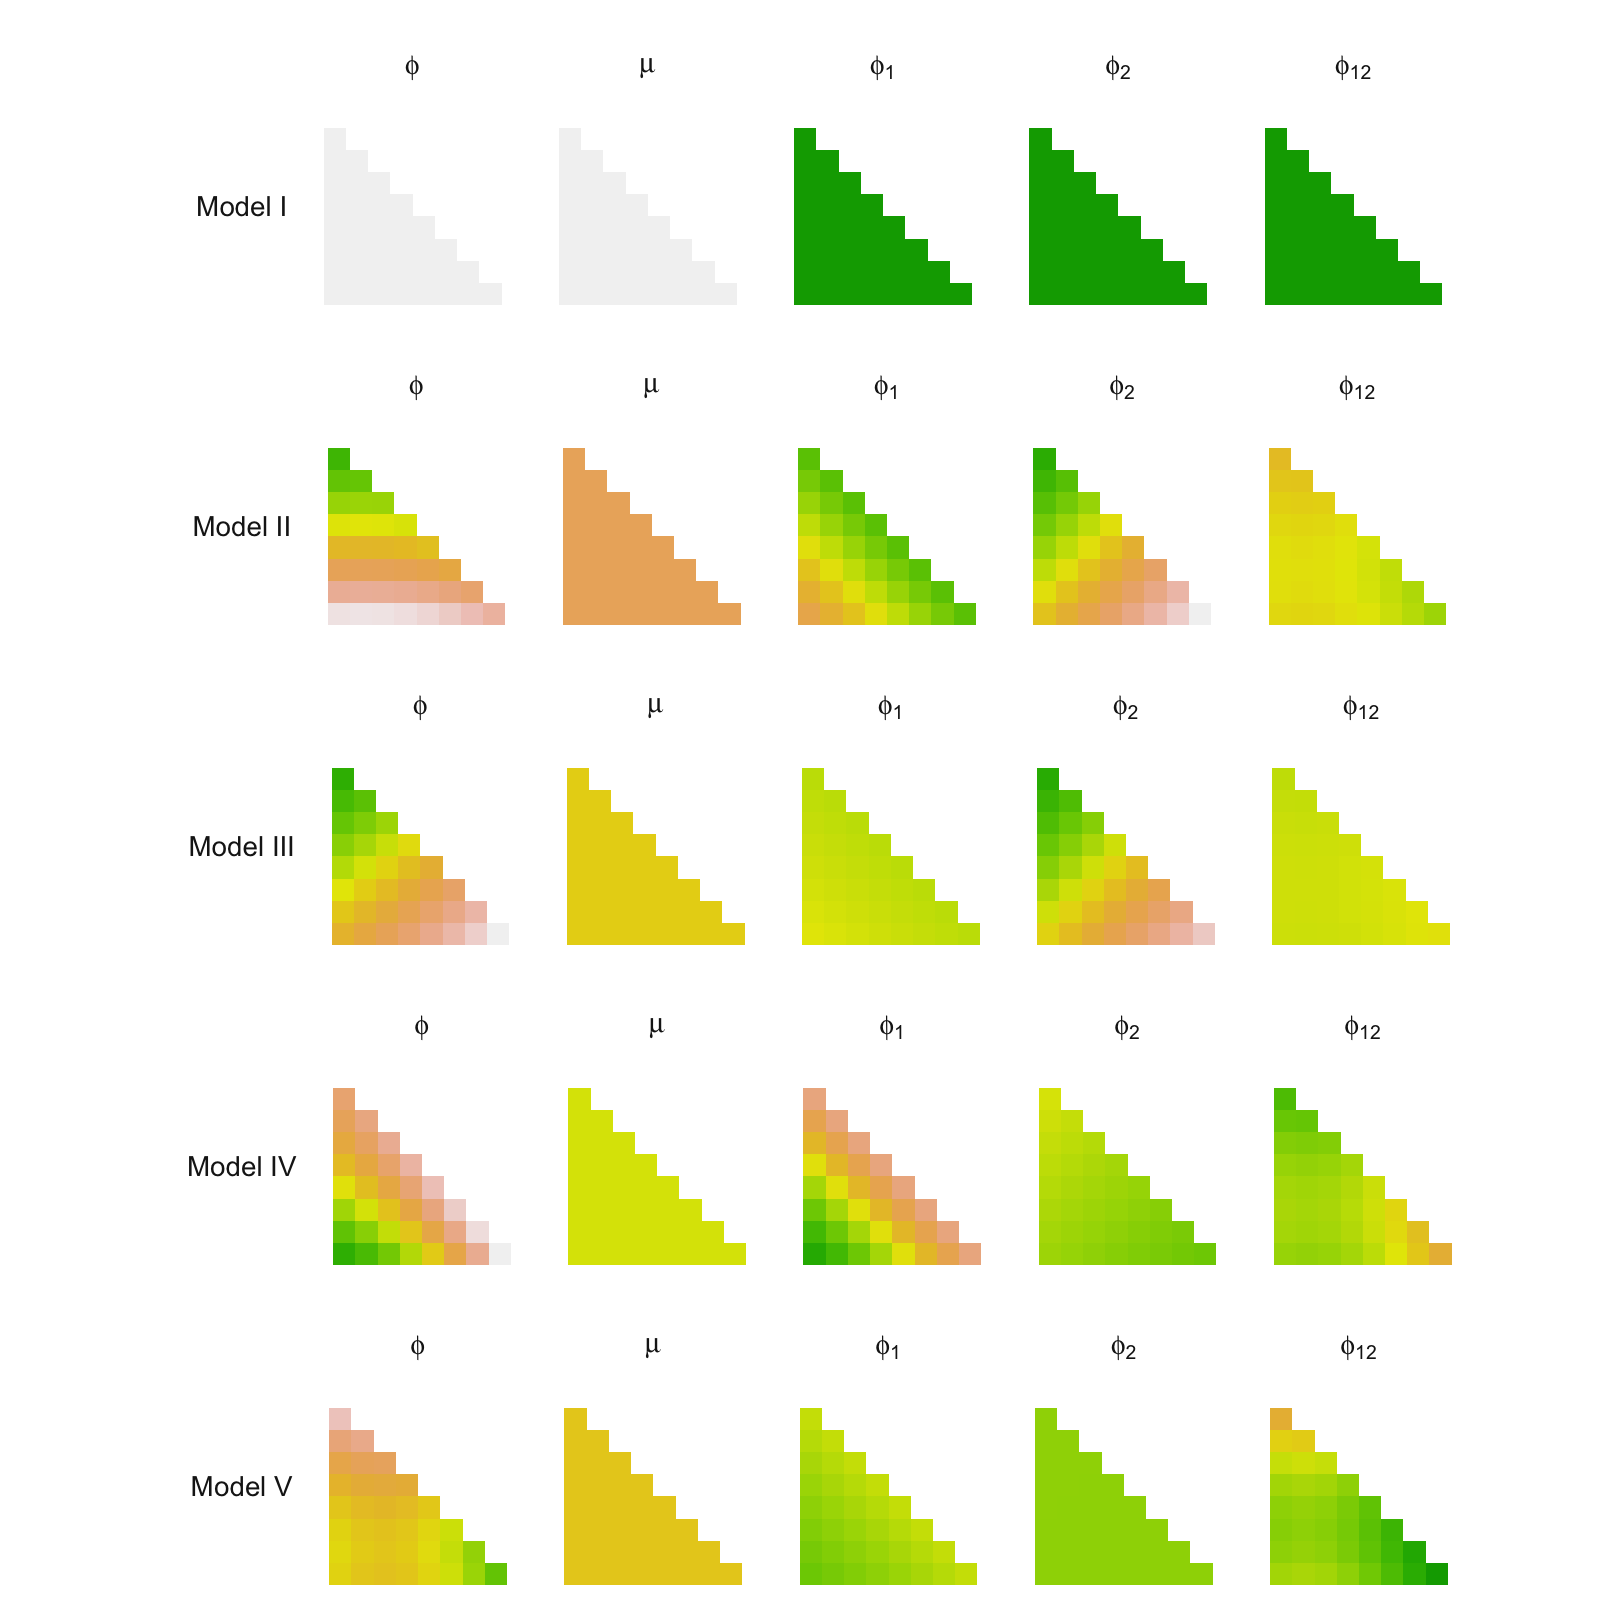
\includegraphics[width = \textwidth]{img/chapter-4/ssanova-estimate-lattice} \label{fig:ssanova-component-lattice}
\end{figure}

\bigskip
The results of the simulations for complete data under entropy loss are presented in Tables~\ref{table:simulation-1-entropy-loss-sigma-1} - \ref{table:simulation-1-entropy-loss-sigma-5}, where the smoothing parameters for our smoothing spline estimator $\hat{\Sigma}_{SS}$ and P-spline estimator $\hat{\Sigma}_{PS}$ are chosen using the unbiased risk estimate. Performance of the estimator when the smoothing parameter is chosen using leave-one-subject-out cross validation is comparable; these results are left to Appendix~\ref{simulation-studies-appendix}. Risk estimates under quadratic loss, while there is not agreement between results every time, qualitatively, they are similar in nature to those with entropy loss and are also presented in Appendix~\ref{simulation-studies-appendix}, Tables~\ref{table:simulation-1-quad-loss-sigma-1}-\ref{table:simulation-1-quad-loss-sigma-5}. Since both loss functions are not standardized, they cannot be compared across dimensions $M$.

\bigskip

In general, our estimators outperform the alternative estimators across the five covariance structures. This is not surprising; the soft thresholding estimator assumes no ordering of the variables of the random vector, which all but one of the generating structures exhibit. The tapering estimator assumes that the absolute value of the covariance decays as $l$ increases; only model IV satisfies this. The parametric estimator based on the modified Cholesky decomposition assumes that $\phi$ can be modeled as a univariate function of $l$, which does not hold for any of the models, save model IV.

\bigskip

The smoothing spline estimator outperforms the P-spline estimator in cases where the underlying covariance structure cannot be modeled as a multiplicative function of $l$ and $m$ - namely, model II. It also does a better job estimating the diagonal structure of model I. In most cases, the optimal difference penalty order for the P-spline under the identity covariance matrix is $d = 0$, which corresponds to a ridge penalty on the B-spline coefficients which could lead to a fitted surface which is not necessarily smooth. 

\bigskip

Treating the differencing order as an additional tuning parameter is advantageous since selecting the search for the optimal set of smoothing parameters is much easier when the true function belongs to the null space of the penalty. The P-spline estimator outperforms the smoothing spline estimator under models IV and V, likely due to this advantage. While the surface of the Cholesky factor of model IV is smooth, value of the function changes very quickly in distance from the diagonal. The local support of the B-spline basis functions aids in the P-spline estimator's ability to accommodate such fast oscillations in surface. The same can be said for model III, which is not smooth in $l = t - s$.
 
\bigskip
%%%%%%%%%%%%%%%%%%%%%%%%%%%%%%%%%%%%%%%%%%%%%%%%%%%%%%%%%%%%%%%%%%%%%%%%%%%%%%%%%%%%%%%%%%%%%%%%
%%%%%%%%%%%%%%%%%%%%%%%%%%%%%%%%%%%%%%%%%%%%%%%%%%%%%%%%%%%%%%%%%%%%%%%%%%%%%%%%%%%%%%%%%%%%%%%%
\setlength{\dashlinedash}{0.5pt}
\setlength{\dashlinegap}{1pt}
\setlength{\arrayrulewidth}{0.2pt}
%\subfile{chapter-4-subfiles/simulation-study-1-entropy-table-model-1}
% latex table generated in R 3.4.3 by xtable 1.8-2 package
% Tue Mar  6 10:27:03 2018
\begin{table}[H]
\centering
\caption{\textit{Multivariate normal simulations for Model I. Estimated entropy risk is reported for our smoothing spline ANOVA estimator and P-spline estimator, the oracle estimator for each covariance structure, the parametric polynomial estimator of Pan and MacKenzie (2003), the sample covariance matrix, the tapered sample covariance matrix, and the soft thresholding estimator.}}
\begin{tabular}{lrrrrrrrr}
 & $M$ & $\hat{\Sigma}_{oracle}$& $\hat{\Sigma}_{SS}$& $\hat{\Sigma}_{PS}$ & $\hat{\Sigma}_{poly}$ & $S$ &$S^\omega$& $S^\lambda$ \\ 
  \hline
$N = 50$ & 10 &0.0135 & 0.0685 & 0.1261 &  0.1102 & 1.2047 & 0.5369 & 1.1742 \\ 
   & $20$ & 0.0229 & 0.0834 & 0.1713 &  0.1096 & 4.9850 & 1.3957 & 4.7796 \\ 
   & $30$ & 0.0196 & 0.1102 & 0.1969 &  0.1127 & 12.5517 & 2.8019 & 11.3175 \\ 
 $N = 100$ & $10$ & 0.0105 & 0.0451 & 0.0671 & 0.0531 & 0.5685 & 0.2045 & 0.5236 \\ 
   & $20$ & 0.0105 &0.0425 & 0.0965 &  0.0512 & 2.2831 & 0.5724 & 2.1358 \\ 
   & $30$ &0.0139 & 0.0431 & 0.1148 &  0.0472 & 5.2770 & 1.2430 & 4.9126 \\ 
   \hline
\end{tabular}
\label{table:simulation-1-entropy-loss-sigma-1}
\end{table}


%%%%%%%%%%%%%%%%%%%%%%%%%%%%%%%%%%%%%%%%%%%%%%%%%%%%%%%%%%%%%%%%%%%%%%%%%%%%%%%%%%%%%%%%%%%%%%%%
%%%%%%%%%%%%%%%%%%%%%%%%%%%%%%%%%%%%%%%%%%%%%%%%%%%%%%%%%%%%%%%%%%%%%%%%%%%%%%%%%%%%%%%%%%%%%%%%
% latex table generated in R 3.4.3 by xtable 1.8-2 package
% Tue Mar  6 10:27:30 2018

\begin{table}[H]
\centering
\caption{\textit{Multivariate normal simulations for model II.}}
\begin{tabular}{lrrrrrrrr}
 & $M$ &$\hat{\Sigma}_{oracle}$& $\hat{\Sigma}_{SS}$& $\hat{\Sigma}_{PS}$ & $\hat{\Sigma}_{poly}$ & $S$ &$S^\omega$& $S^\lambda$ \\ 
  \hline
   $N = 50$ & $10$ & 0.0581 &  0.0689 & 0.3423 &4.7673 & 1.2832 & 1.4644 & 1.1770 \\ 
   & $20$ &0.0439 & 0.0581 & 1.3640 &  97.2334 & 5.1665 & 21.6407 & 39.3522 \\ 
     & $30$ & 0.0627 & 0.0811 & 2.6485 &  153.9665 & 12.3582 & 55.3674 & 133.9980 \\ 
  $N = 100$ & 10 &  0.0386 & 0.0457 & 0.2945 & 4.7911 & 0.5812 & 0.8335 & 0.5628 \\ 
    & $20$ & 0.0269 & 0.0416 & 1.2875 &  98.1989 & 2.3364 & 10.1841 & 10.0864 \\ 
    & $30$ &  0.0288 & 0.0367 & 2.4365 & 158.2480 & 5.2389 & 33.5207 & 62.5030 \\ 
   \hline
\end{tabular}
\label{table:simulation-1-entropy-loss-sigma-2}
\end{table}


%%%%%%%%%%%%%%%%%%%%%%%%%%%%%%%%%%%%%%%%%%%%%%%%%%%%%%%%%%%%%%%%%%%%%%%%%%%%%%%%%%%%%%%%%%%%%%%%
%%%%%%%%%%%%%%%%%%%%%%%%%%%%%%%%%%%%%%%%%%%%%%%%%%%%%%%%%%%%%%%%%%%%%%%%%%%%%%%%%%%%%%%%%%%%%%%%
%\subfile{chapter-4-subfiles/simulation-study-1-entropy-table-model-2}
%\subfile{chapter-4-subfiles/simulation-study-1-entropy-table-model-3}
% latex table generated in R 3.4.3 by xtable 1.8-2 package
% Tue Mar  6 10:27:35 2018


\begin{table}[H]
\centering
\caption{\textit{Multivariate normal simulations for model III.} }
\begin{tabular}{lrrrrrrrr}
 & $M$ &$\hat{\Sigma}_{oracle}$&  $\hat{\Sigma}_{SS}$& $\hat{\Sigma}_{PS}$ &$\hat{\Sigma}_{poly}$ & $S$ &$S^\omega$& $S^\lambda$ \\ 
   \hline
 $N = 50$ & 10 & 0.0619 & 0.3296 & 0.1065 & 3.0108 & 1.2030 & 1.1460 & 1.1467 \\ 
      & $20$ &0.0695 & 1.1100 & 0.2555 &  62.7522 & 4.9824 & 17.2244 & 14.9189 \\ 
    & $30$ &0.0576 & 2.3215 & 0.6242 &  1091.1933 & 12.4792 & 49.9135 & 121.7795 \\ 
     $N = 100$ & $10$ & 0.0268 &  0.2904 & 0.0579 &3.0383 & 0.5699 & 0.5545 & 0.5371 \\ 
     & $20$ & 0.0275 & 1.1963 & 0.2011 & 62.8960 & 2.2700 & 11.8274 & 9.5217 \\ 
    & $30$ &  0.0221 & 2.2811 & 0.3845 &1105.0449 & 5.2234 & 29.1693 & 60.3529 \\ 
   \hline
\end{tabular}
\label{table:simulation-1-entropy-loss-sigma-3}
\end{table}

%%%%%%%%%%%%%%%%%%%%%%%%%%%%%%%%%%%%%%%%%%%%%%%%%%%%%%%%%%%%%%%%%%%%%%%%%%%%%%%%%%%%%%%%%%%%%%%%
%%%%%%%%%%%%%%%%%%%%%%%%%%%%%%%%%%%%%%%%%%%%%%%%%%%%%%%%%%%%%%%%%%%%%%%%%%%%%%%%%%%%%%%%%%%%%%%%
%\subfile{chapter-4-subfiles/simulation-study-1-entropy-table-model-4}
% latex table generated in R 3.4.3 by xtable 1.8-2 package
% Tue Mar  6 10:27:39 2018
\begin{table}[H]
\centering
\caption{\textit{Multivariate normal simulations for model IV.}}
\begin{tabular}{lrrrrrrrr}
 & $M$ & $\hat{\Sigma}_{oracle}$ & $\hat{\Sigma}_{SS}$& $\hat{\Sigma}_{PS}$ & $\hat{\Sigma}_{poly}$ & $S$ &$S^\omega$& $S^\lambda$ \\ 
  \hline
 $N = 50$ & $10$ & 0.0217 & 0.3348 & 0.1966 & 0.7144 & 1.2218 & 0.7397 & 1.1921 \\ 
   & $20$ &0.0286 & 0.9177 & 0.3499 &  1.4588 & 4.9091 & 1.9786 & 4.9206 \\ 
       & $30$ &  0.0283 &1.5992 & 0.5100 & 2.2173 & 12.6114 & 3.7440 & 12.1489 \\ 
     $N = 100$ & 10 & 0.0125 & 0.3047 & 0.2237 &  0.6958 & 0.5570 & 0.3168 & 0.5515 \\ 
       & $20$ &0.0105 & 0.8911 & 0.3704 &  1.4813 & 2.2659 & 0.9365 & 2.2474 \\ 
       & $30$ & 0.0134 & 1.5213 & 0.5282 & 2.2228 & 5.2106 & 1.9312 & 5.2111 \\ 
   \hline
\end{tabular} 
\label{table:simulation-1-entropy-loss-sigma-4}
\end{table}

%%%%%%%%%%%%%%%%%%%%%%%%%%%%%%%%%%%%%%%%%%%%%%%%%%%%%%%%%%%%%%%%%%%%%%%%%%%%%%%%%%%%%%%%%%%%%%%%
%%%%%%%%%%%%%%%%%%%%%%%%%%%%%%%%%%%%%%%%%%%%%%%%%%%%%%%%%%%%%%%%%%%%%%%%%%%%%%%%%%%%%%%%%%%%%%%%
%\subfile{chapter-4-subfiles/simulation-study-1-entropy-table-model-5}
% latex table generated in R 3.4.3 by xtable 1.8-2 package
% Tue Mar  6 10:27:42 2018
\begin{table}[H]
\centering
\caption{\textit{Multivariate normal simulations for model V.}}
\begin{tabular}{lrrrrrrrr}
 & $M$ &$\hat{\Sigma}_{oracle}$&$\hat{\Sigma}_{SS}$& $\hat{\Sigma}_{PS}$ & $\hat{\Sigma}_{poly}$ & $S$ &$S^\omega$& $S^\lambda$ \\ 
  \hline
 $N = 50$ & $10$ &  0.0986 &0.2769 & 0.2464 & 1.2420 & 1.2023 & 18.5222 & 2.9824 \\ 
  & $20$ &0.2512 & 0.7514 & 0.8772 &  2.8557 & 5.0195 & 34.6618 & 13.8690 \\ 
  & $30$ &  0.2641& 1.1776 & 0.9791  & 4.5791 & 12.3460 & 46.5437 & 26.1364 \\ 
 $N = 100$ & 10 &0.0520 & 0.2416 & 0.1722 &  1.1491 & 0.5821 & 16.4081 & 1.7397 \\ 
  & $20$ & 0.0827 & 0.7286 & 0.2965 &  2.9080 & 2.2918 & 32.5295 & 5.4649 \\ 
   & $30$ &  0.1799 & 1.1813 & 0.4291 & 4.4402 & 5.2197 & 39.2914 & 15.4295 \\ 
   \hline
\end{tabular}\label{table:simulation-1-entropy-loss-sigma-5}
\end{table}


%\subfile{chapter-4-subfiles/simulation-study-1-entropy-single-table}
%%%%%%%%%%%%%%%%%%%%%%%%%%%%%%%%%%%%%%%%%%%%%%%%%%%%%%%%%%%%%%%%%%%%%%%%%%%%%%%%%%%%%%%%%%%%%%%%
%%%%%%%%%%%%%%%%%%%%%%%%%%%%%%%%%%%%%%%%%%%%%%%%%%%%%%%%%%%%%%%%%%%%%%%%%%%%%%%%%%%%%%%%%%%%%%%%
%%%%%%%%%%%%%%%%%%%%%%%%%%%%%%%%%%%%%%%%%%%%%%%%%%%%%%%%%%%%%%%%%%%%%%%%%%%%%%%%%%%%%%%%%%%%%%%%
%%%%%%%%%%%%%%%%%%%%%%%%%%%%%%%%%%%%%%%%%%%%%%%%%%%%%%%%%%%%%%%%%%%%%%%%%%%%%%%%%%%%%%%%%%%%%%%%
%%%%%%%%%%%%%%%%%%%%%%%%%%%%%%%%%%%%%%%%%%%%%%%%%%%%%%%%%%%%%%%%%%%%%%%%%%%%%%%%%%%%%%%%%%%%%%%%
\subsection{Performance with Irregularly Sampled Data}
%%%%%%%%%%%%%%%%%%%%%%%%%%%%%%%%%%%%%%%%%%%%%%%%%%%%%%%%%%%%%%%%%%%%%%%%%%%%%%%%%%%%%%%%%%%%%%%%
%%%%%%%%%%%%%%%%%%%%%%%%%%%%%%%%%%%%%%%%%%%%%%%%%%%%%%%%%%%%%%%%%%%%%%%%%%%%%%%%%%%%%%%%%%%%%%%%
%%%%%%%%%%%%%%%%%%%%%%%%%%%%%%%%%%%%%%%%%%%%%%%%%%%%%%%%%%%%%%%%%%%%%%%%%%%%%%%%%%%%%%%%%%%%%%%%
%%%%%%%%%%%%%%%%%%%%%%%%%%%%%%%%%%%%%%%%%%%%%%%%%%%%%%%%%%%%%%%%%%%%%%%%%%%%%%%%%%%%%%%%%%%%%%%%
%%%%%%%%%%%%%%%%%%%%%%%%%%%%%%%%%%%%%%%%%%%%%%%%%%%%%%%%%%%%%%%%%%%%%%%%%%%%%%%%%%%%%%%%%%%%%%%%
%\subfile{chapter-4-subfiles/chapter-4-missing-data-study-discussion}

Estimated risk under entropy loss is given in Tables~\ref{table:simulation-study-2-entropy-risk-model-1} - \ref{table:simulation-study-2-entropy-risk-model-5}.  Risk estimates under quadratic loss echo in sentiment and are left to Appendix~\ref{simulation-studies-appendix}, Tables~\ref{table:simulation-study-2-quad-risk-model-1} - \ref{table:simulation-study-2-quad-risk-model-5}. Neither model selection perform better than the other across all of the simulation settings. This might suggest that when the estimated innovation variances are close to the true variances of the prediction residuals, using the unbiased risk estimate with the working residuals as substitute for the relative error is a reasonable approach to modeling. Performance degradation of the estimator in the presence of missing data is highly dependent on the underlying structure of the Cholesky factor of the inverse covariance matrix. For Models I and IV, the identity matrix and the rational quadratic covariance model, performance remains fairly stable as the proportion of missing data increases. The estimator exhibits similar degrees of performance degradation under Models II, III, and V.  Interestingly, these models (with the exception of Model III, which is a special case) have true varying coefficient functions which are naturally parameterized as functions of $t$, while the models under which the performance remain stable across increasing proportions of missing data are naturally parameterized in terms of $l$. 

%%%%%%%%%%%%%%%%%%%%%%%%%%%%%%%%%%%%%%%%%%%%%%%%%%%%%%%%%%%%%%%%%%%%%%%%%%%%%%%%%%%%%%%%%%%%%%%%
%%%%%%%%%%%%%%%%%%%%%%%%%%%%%%%%%%%%%%%%%%%%%%%%%%%%%%%%%%%%%%%%%%%%%%%%%%%%%%%%%%%%%%%%%%%%%%%%
%%%%%%%%%%%%%%%%%%%%%%%%%%%%%%%%%%%%%%%%%%%%%%%%%%%%%%%%%%%%%%%%%%%%%%%%%%%%%%%%%%%%%%%%%%%%%%%%
%%%%%%%%%%%%%%%%%%%%%%%%%%%%%%%%%%%%%%%%%%%%%%%%%%%%%%%%%%%%%%%%%%%%%%%%%%%%%%%%%%%%%%%%%%%%%%%%
%%%%%%%%%%%%%%%%%%%%%%%%%%%%%%%%%%%%%%%%%%%%%%%%%%%%%%%%%%%%%%%%%%%%%%%%%%%%%%%%%%%%%%%%%%%%%%%%
\bigskip
\setlength{\dashlinedash}{0.5pt}
\setlength{\dashlinegap}{1pt}
\setlength{\arrayrulewidth}{0.2pt}

% latex table generated in R 3.4.3 by xtable 1.8-2 package
% Wed Mar 21 09:46:43 2018
\begin{table}[H]
\centering
\caption{\textit{Model 1: Entropy risk estimates and corresponding standard errors 
                            for the MCD smoothing spline ANOVA estimator via 100 simulated multivariate
                            normal samples of size $N = 50$
                            when 0\%, 10\%, 20\%, and 30\% of the data are missing for each subject. Risk is reported for the estimator constructed using
                            the unbiased risk estimate and leave-one-subject-out cross validation for smoothing parameter selection.} }
\label{table:simulation-study-2-entropy-risk-model-1}
\begin{tabular}{lrrlrl}
   $M$ & \% missing & \multicolumn{2} {c} {$\Delta_2(\hat{\Sigma}^{U}_{SS})$} & \multicolumn{2} {c} {$\Delta_2(\hat{\Sigma}^{V^*}_{SS})$}\\ \hline
10 & 0.0 & 0.06854186 & (0.0065) & 0.0822183 & (0.0075) \\ 
   & 0.1 & 0.08895763 & (0.0080) & 0.0997540 & (0.0083) \\ 
   & 0.2 & 0.08474403 & (0.0069) & 0.1257789 & (0.0110) \\ 
   & 0.3 & 0.14281452 & (0.0114) & 0.1552415 & (0.0142) \\ 
   \hline
20 & 0.0 & 0.08337738 & (0.0056) & 0.0924326 & (0.0167) \\ 
   & 0.1 & 0.10467926 & (0.0072) & 0.3019903 & (0.1922) \\ 
   & 0.2 & 0.13920223 & (0.0076) & 0.2099852 & (0.0308) \\ 
   & 0.3 & 0.17160295 & (0.0088) & 0.3784635 & (0.1054) \\ 
   \hline
\end{tabular}
\end{table}


%%%%%%%%%%%%%%%%%%%%%%%%%%%%%%%%%%%%%%%%%%%%%%%%%%%%%%%%%%%%%%%%%%%%%%%%%%%%%%%%%%%%%%%%%%%%%%%%
%%%%%%%%%%%%%%%%%%%%%%%%%%%%%%%%%%%%%%%%%%%%%%%%%%%%%%%%%%%%%%%%%%%%%%%%%%%%%%%%%%%%%%%%%%%%%%%%
% latex table generated in R 3.4.3 by xtable 1.8-2 package
% Wed Mar 21 09:46:43 2018
\begin{table}[H]
\centering
\caption{\textit{Model 2: Entropy risk estimates and corresponding standard errors.} }
\label{table:simulation-study-2-entropy-risk-model-2}
\begin{tabular}{lrrlrl}
   $M$ & \% missing & \multicolumn{2} {c} {$\Delta_2(\hat{\Sigma}^{U}_{SS})$} & \multicolumn{2} {c} {$\Delta_2(\hat{\Sigma}^{V^*}_{SS})$}\\ \hline
10 & 0.0 & 0.0689091 & (0.0057) & 0.0863937 & (0.0070) \\ 
   & 0.1 & 0.0961388 & (0.0066) & 0.1396364 & (0.0119) \\ 
   & 0.2 & 0.2089429 & (0.0140) & 0.1988000 & (0.0173) \\ 
   & 0.3 & 0.2947206 & (0.0212) & 0.3247143 & (0.0297) \\ 
   \hline
20 & 0.0 & 0.0580730 & (0.0042) & 0.0851086 & (0.0061) \\ 
   & 0.1 & 0.6508269 & (0.0437) & 0.6936141 & (0.0366) \\ 
   & 0.2 & 3.9959421 & (0.2127) & 7.9307772 & (2.6348) \\ 
   & 0.3 & 16.4362761 & (1.3678) & 24.4878411 & (1.5554) \\ 
   \hline
\end{tabular}
\end{table}


%%%%%%%%%%%%%%%%%%%%%%%%%%%%%%%%%%%%%%%%%%%%%%%%%%%%%%%%%%%%%%%%%%%%%%%%%%%%%%%%%%%%%%%%%%%%%%%%
%%%%%%%%%%%%%%%%%%%%%%%%%%%%%%%%%%%%%%%%%%%%%%%%%%%%%%%%%%%%%%%%%%%%%%%%%%%%%%%%%%%%%%%%%%%%%%%%
% latex table generated in R 3.4.3 by xtable 1.8-2 package
% Wed Mar 21 09:46:43 2018
\begin{table}[H]
\centering
\caption{\textit{Model 3: Entropy risk estimates and corresponding standard errors.} }
\label{table:simulation-study-2-entropy-risk-model-3}
\begin{tabular}{lrrlrl}
   $M$ & \% missing & \multicolumn{2} {c} {$\Delta_2(\hat{\Sigma}^{U}_{SS})$} & \multicolumn{2} {c} {$\Delta_2(\hat{\Sigma}^{V^*}_{SS})$}\\ \hline
10 & 0.0 & 0.3295884 & (0.0063) & 0.3463639 & (0.0093) \\ 
   & 0.1 & 0.3442326 & (0.0079) & 0.3555080 & (0.0097) \\ 
   & 0.2 & 0.3922506 & (0.0098) & 0.4231472 & (0.0138) \\ 
   & 0.3 & 0.4518739 & (0.0187) & 0.5270384 & (0.0237) \\ 
   \hline
20 & 0.0 & 1.1100351 & (0.0107) & 1.1312420 & (0.0089) \\ 
   & 0.1 & 1.3867351 & (0.0384) & 1.5369483 & (0.0360) \\ 
   & 0.2 & 4.4685998 & (0.2608) & 4.4221240 & (0.2856) \\ 
   & 0.3 & 13.9195476 & (1.3110) & 16.5667952 & (1.1101) \\ 
   \hline
\end{tabular}
\end{table}

%%%%%%%%%%%%%%%%%%%%%%%%%%%%%%%%%%%%%%%%%%%%%%%%%%%%%%%%%%%%%%%%%%%%%%%%%%%%%%%%%%%%%%%%%%%%%%%%
%%%%%%%%%%%%%%%%%%%%%%%%%%%%%%%%%%%%%%%%%%%%%%%%%%%%%%%%%%%%%%%%%%%%%%%%%%%%%%%%%%%%%%%%%%%%%%%%
% latex table generated in R 3.4.3 by xtable 1.8-2 package
% Wed Mar 21 09:46:43 2018
\begin{table}[H]
\centering
\caption{\textit{Model 4: Entropy risk estimates and corresponding standard errors.} }
\label{table:simulation-study-2-entropy-risk-model-4}
\begin{tabular}{lrrlrl}
   $M$ & \% missing & \multicolumn{2} {c} {$\Delta_2(\hat{\Sigma}^{U}_{SS})$} & \multicolumn{2} {c} {$\Delta_2(\hat{\Sigma}^{V^*}_{SS})$}\\ \hline
10 & 0.0 & 0.3347516 & (0.0056) & 0.3420091 & (0.0063) \\ 
   & 0.1 & 0.3561451 & (0.0076) & 0.3536609 & (0.0079) \\ 
   & 0.2 & 0.3901020 & (0.0111) & 0.3884112 & (0.0098) \\ 
   & 0.3 & 0.4395183 & (0.0139) & 0.4399004 & (0.0162) \\ 
   \hline
20 & 0.0 & 0.9176583 & (0.0083) & 0.9345338 & (0.0074) \\ 
   & 0.1 & 0.9316105 & (0.0101) & 0.9592996 & (0.0116) \\ 
   & 0.2 & 0.9620128 & (0.0090) & 1.0192813 & (0.0201) \\ 
   & 0.3 & 1.0339355 & (0.0123) & 1.0986877 & (0.0680) \\ 
   \hline
\end{tabular}
\end{table}


%%%%%%%%%%%%%%%%%%%%%%%%%%%%%%%%%%%%%%%%%%%%%%%%%%%%%%%%%%%%%%%%%%%%%%%%%%%%%%%%%%%%%%%%%%%%%%%%
%%%%%%%%%%%%%%%%%%%%%%%%%%%%%%%%%%%%%%%%%%%%%%%%%%%%%%%%%%%%%%%%%%%%%%%%%%%%%%%%%%%%%%%%%%%%%%%%
% latex table generated in R 3.4.3 by xtable 1.8-2 package
% Wed Mar 21 09:46:43 2018
\begin{table}[H]
\centering
\caption{\textit{Model 5: Entropy risk estimates and corresponding standard errors.} }
\label{table:simulation-study-2-entropy-risk-model-5}
\begin{tabular}{lrrlrl}
   $M$ & \% missing & \multicolumn{2} {c} {$\Delta_2(\hat{\Sigma}^{U}_{SS})$} & \multicolumn{2} {c} {$\Delta_2(\hat{\Sigma}^{V^*}_{SS})$}\\ \hline
10 & 0.0 & 0.2768874 & (0.0054) & 0.2855551 & (0.0090) \\ 
   & 0.1 & 0.4139307 & (0.0160) & 0.4290270 & (0.0161) \\ 
   & 0.2 & 0.8698641 & (0.0448) & 0.9289941 & (0.0586) \\ 
   & 0.3 & 1.8588993 & (0.1172) & 2.1368920 & (0.1284) \\ 
   \hline
20 & 0.0 & 0.7514261 & (0.0053) & 0.7609570 & (0.0063) \\ 
   & 0.1 & 1.2295533 & (0.0522) & 1.1317517 & (0.0294) \\ 
   & 0.2 & 2.5715989 & (0.0976) & 2.4974678 & (0.1081) \\ 
   & 0.3 & 7.4723499 & (0.3235) & 6.8275522 & (0.3006) \\ 
   \hline
\end{tabular}
\end{table}


%%%%%%%%%%%%%%%%%%%%%%%%%%%%%%%%%%%%%%%%%%%%%%%%%%%%%%%%%%%%%%%%%%%%%%%%%%%%%%%%%%%%%%%%%%%%%%%%
%%%%%%%%%%%%%%%%%%%%%%%%%%%%%%%%%%%%%%%%%%%%%%%%%%%%%%%%%%%%%%%%%%%%%%%%%%%%%%%%%%%%%%%%%%%%%%%%

%\subfile{chapter-4-subfiles/chapter-4-numerical-discussion-2}
%%%%%%%%%%%%%%%%%%%%%%%%%%%%%%%%%%%%%%%%%%%%%%%%%%%%%%%%%%%%%%%%%%%%%%%%%%%%%%%%%%%%%%%%%%%%%%%%
%%%%%%%%%%%%%%%%%%%%%%%%%%%%%%%%%%%%%%%%%%%%%%%%%%%%%%%%%%%%%%%%%%%%%%%%%%%%%%%%%%%%%%%%%%%%%%%%
%%%%%%%%%%%%%%%%%%%%%%%%%%%%%%%%%%%%%%%%%%%%%%%%%%%%%%%%%%%%%%%%%%%%%%%%%%%%%%%%%%%%%%%%%%%%%%%%
%%%%%%%%%%%%%%%%%%%%%%%%%%%%%%%%%%%%%%%%%%%%%%%%%%%%%%%%%%%%%%%%%%%%%%%%%%%%%%%%%%%%%%%%%%%%%%%%
%%%%%%%%%%%%%%%%%%%%%%%%%%%%%%%%%%%%%%%%%%%%%%%%%%%%%%%%%%%%%%%%%%%%%%%%%%%%%%%%%%%%%%%%%%%%%%%%


%\bibliography{../Master}
%\end{document}
       

\chapter{Data Analysis} \label{data-analysis-chapter}

\cite{kenward1987method} reported an experiment designed to investigate the impact of the control of intestinal parasites in cattle. The grazing season runs from spring to autumn, during which cattle can potentially ingest roundworm larvae which develop from eggs deposited around the pasture from feces of previously infected cattle. Once infected, the animal is deprived of nutrients and immune resistance to disease is suppressed which can significantly impact animal growth. Monitoring the effect of a treatment for the disease requires repeated weight measurements on animals over the grazing season. 

\bigskip

To compare two methods for controlling the disease, say treatment A and treatment B, each of 60 cattle were assigned randomly to two groups, each of size 30. Animal subjects were put out to pasture at the start of grazing season, with each member of the groups receiving one of the two treatments. Animals were weighed $p = 11$ times over a 133-day period; the first 10 measurements on each animal were made at two-week intervals and the final measurement was made one week later. Weights were recorded to the nearest kilogram, and measurement times were common across animals. The longitudinal dataset is balanced, as there were no missing observations for any of the experimental units. Observed weights are shown in Figure~\ref{fig:cattle-weights-by-trt}.

\begin{center}  
\begin{figure}[H] 
\begin{center}
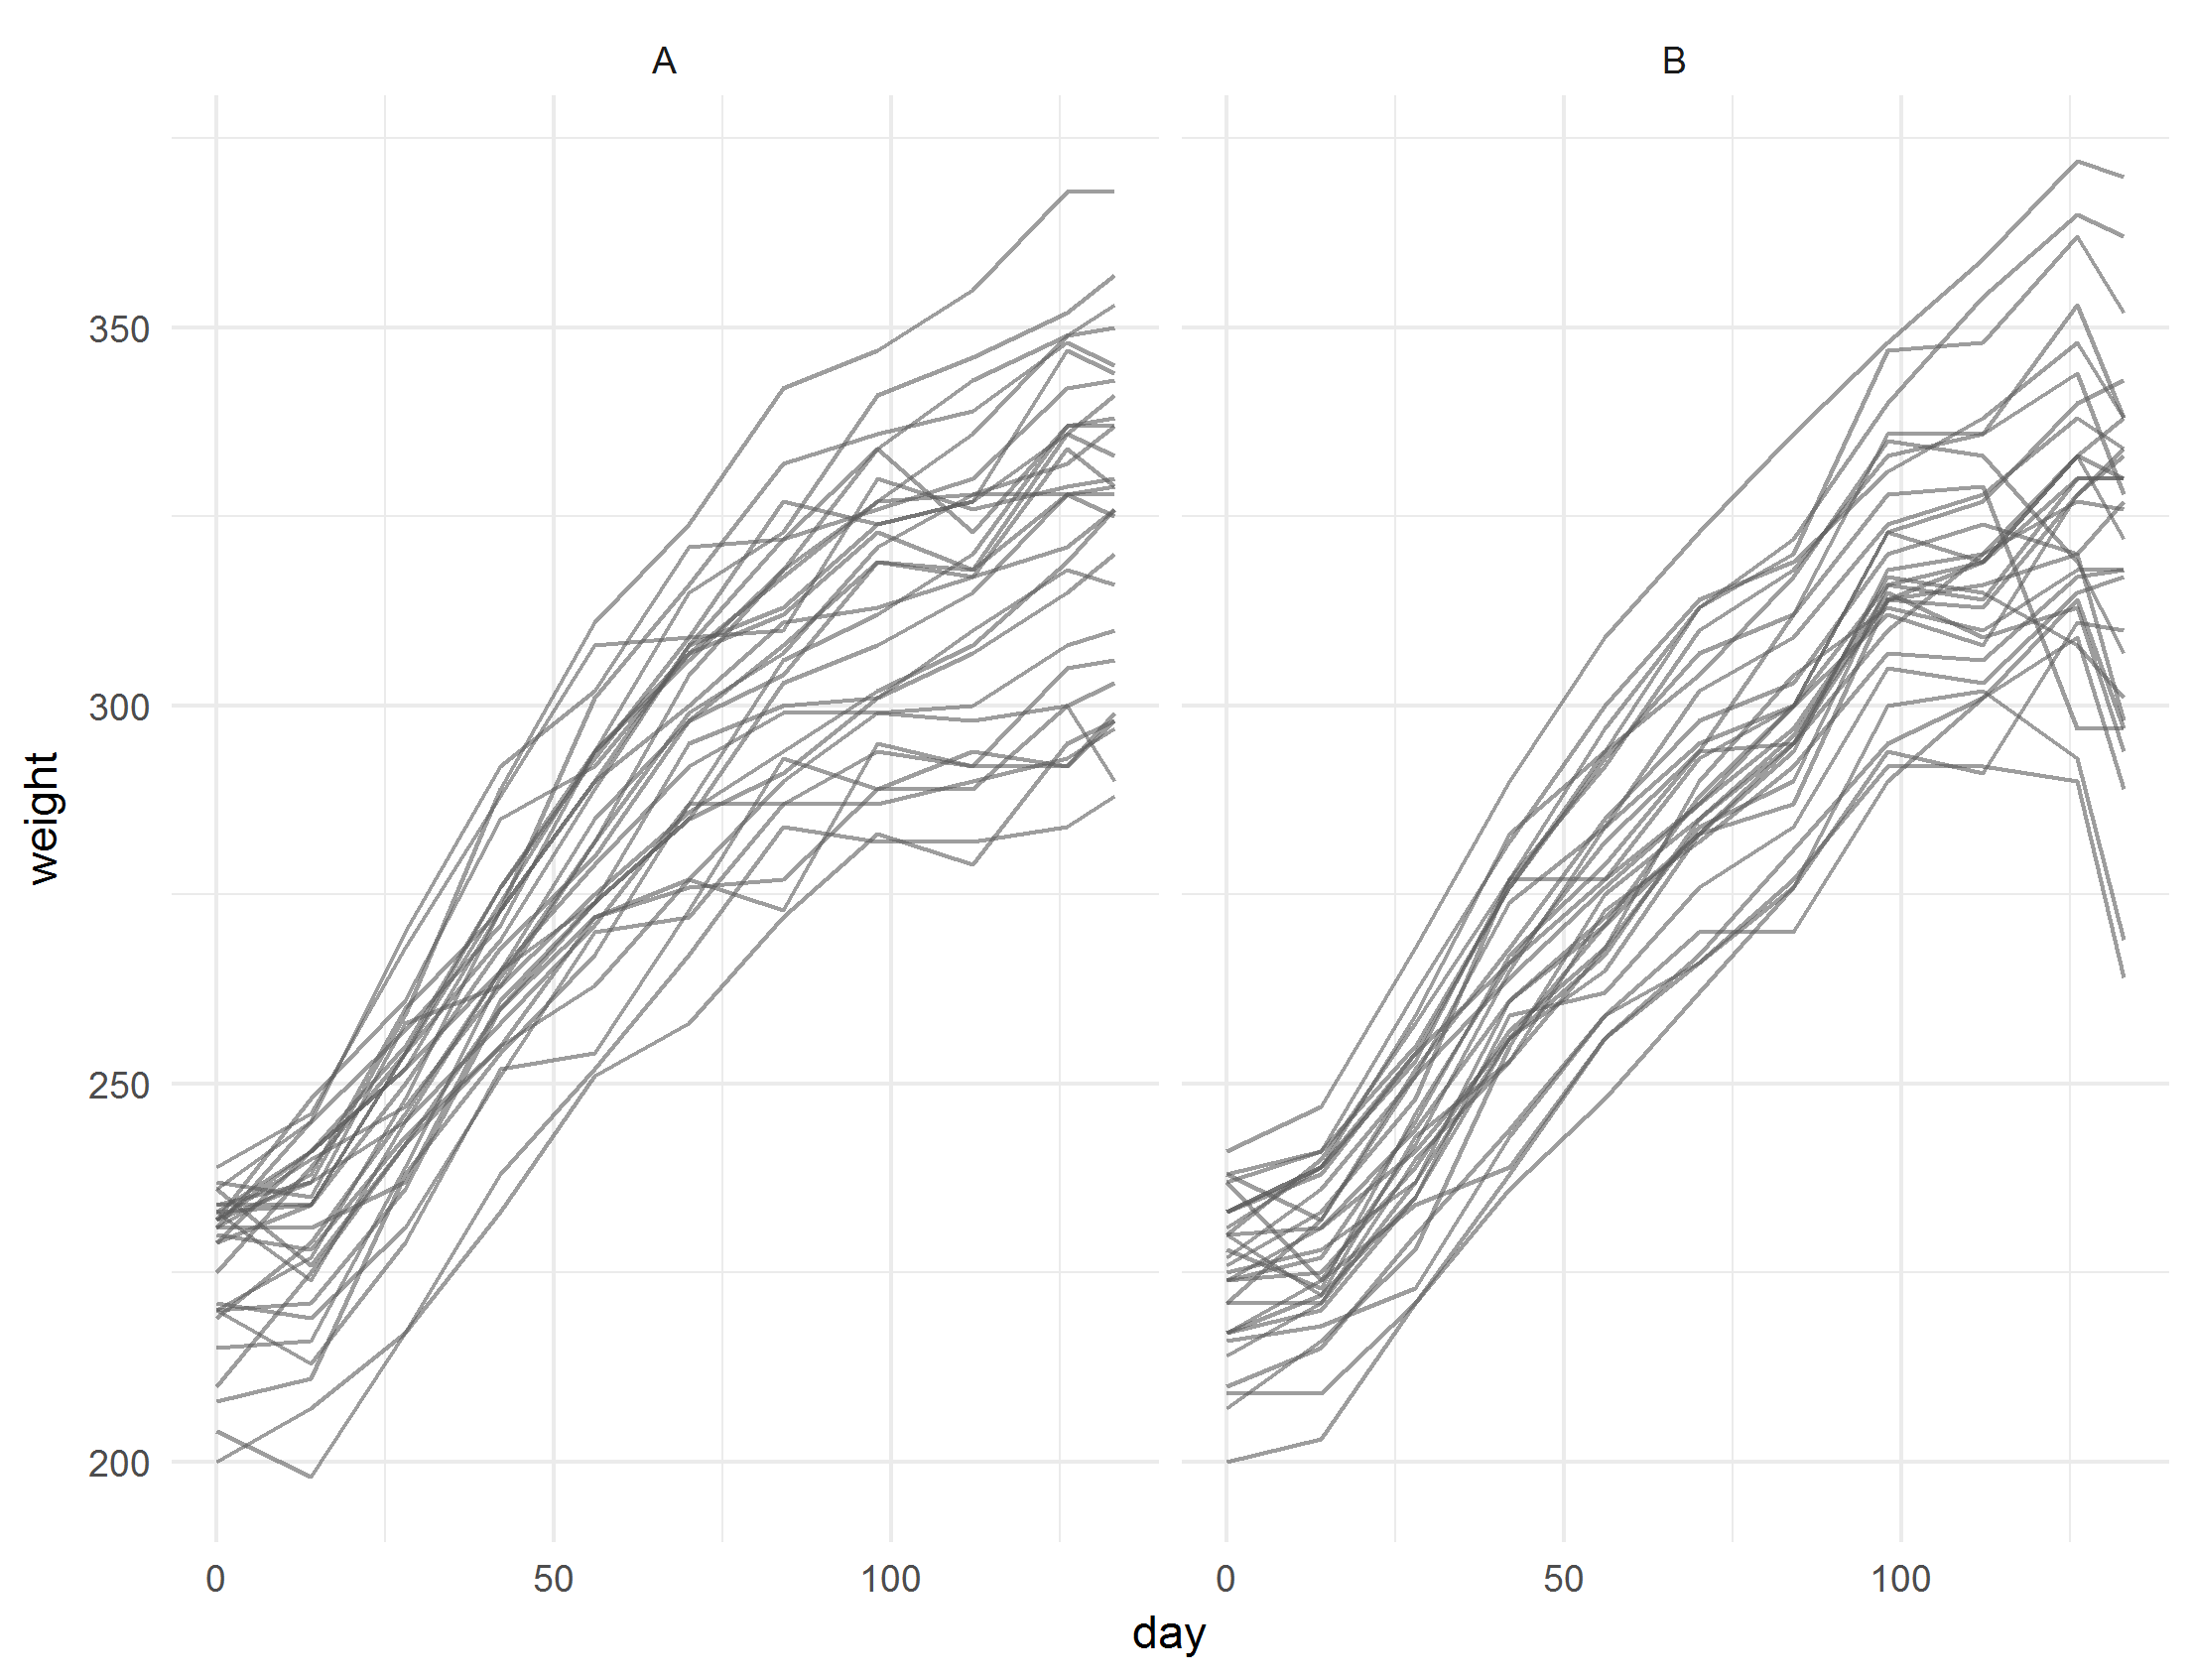
\includegraphics[width = .9\textwidth, height = 5in]{img/cattle/cattle-weights-vs-time-by-trt}
\caption{\textit{Subject-specific weight curves over time for treatment groups A and B.}}\label{fig:cattle-weights-by-trt}
\end{center}
\end{figure} 
\end{center}

We see an upward trend in weights over time, with variance in weights increasing over time for both groups. Treatment group B demonstrates a sharp decrease in the final weight measurement. The analysis of the same dataset provided by \cite{zimmerman1997structured} rejected equality of the two covariance matrices corresponding to treatment group using the classical likelihood ratio test, making it reasonable to study each treatment group's covariance matrix separately. Following \cite{pan2017jmcm}, \cite{zhang2015joint}, and \cite{pourahmadi1999joint}, we analyze the data from the $N = 30$ cattle assigned to treatment group A, which we assume share a common $11 \times 11$ covariance matrix $\Sigma$. The left profile plot in Figure~\ref{fig:cattle-weights-by-trt} of the weights for units in treatment group A shows a clear upward trend in weights;  variances appear to increase over time, suggesting that the covariance structure is nonstationary.

\bigskip

The nonstationarity suggested in Figure~\ref{fig:cattle-weights-by-trt} is also supported by the sample correlations given in Table~\ref{table:cattleA-sample-correlations}; correlations within the subdiagonals are not constant and increase over time, a secondary indication that a stationary covariance is not appropriate for the data.  Table~\ref{table:sample-regressogram-garps} gives the sample generalised autoregressive parameters and the innovation variances, which are plotted in Figure~\ref{fig:cattleA-regressogram} and Figure~\ref{fig:cattleA-innovation-variogram} respectively. 

\begin{table}[H] 
\begin{center}
\begin{tabular}{r|rrrrrrrrrrr}
& \multicolumn{11}{c}{day}\\
&&&&&&&&&&\\
& 0 & 14 & 28 & 42 & 56 & 70 & 84 & 98& 112& 126 &133\\
  \hline\noalign{\smallskip} 
0 & 1.00  \\ 
  14 & 0.82 & 1.00  \\ 
  28 & 0.76 & 0.91 & 1.00 & \\ 
  42 & 0.65 & 0.86 & 0.93 & 1.00 &  \\ 
  56 & 0.63 & 0.83 & 0.89 & 0.93 & 1.00 &  \\ 
  70 & 0.58 & 0.75 & 0.85 & 0.90 & 0.94 & 1.00 & \\ 
  84 & 0.51 & 0.64 & 0.75 & 0.80 & 0.85 & 0.92 & 1.00 &\\ 
  98 & 0.52 & 0.68 & 0.77 & 0.82 & 0.88 & 0.93 & 0.92 & 1.00 & \\ 
  112 & 0.51 & 0.61 & 0.71 & 0.74 & 0.81 & 0.89 & 0.92 & 0.96 & 1.00 & \\ 
  120 & 0.46 & 0.59 & 0.69 & 0.70 & 0.77 & 0.85 & 0.86 & 0.94 & 0.96 & 1.00 &  \\ 
  133 & 0.46 & 0.56 & 0.67 & 0.67 & 0.74 & 0.81 & 0.84 & 0.91 & 0.95 & 0.98 & 1.00 \\ 
   \hline
\end{tabular}
\caption{\textit{Cattle data: treatment group A sample correlations.}}\label{table:cattleA-sample-correlations}
\end{center}
\end{table}


\begin{table}[H] 
\begin{center}
\begin{tabular}{lc|ccccccccccc|cr}
 \multicolumn{14}{c}{day} \\
&&&&&&&&&&&&\\
& &  0 & 14 & 28 & 42 & 56 & 70 & 84 & 98 & 112 & 126 & 133  \\ 
  \cline{2-13}\noalign{\smallskip}  
&0 & 1 & &&&&&&&&& & 4.673& \\ 
&  14& 1.00 & 1&&&&&&&&&& 3.939 &\\ 
&  28 & 0.04 & 0.90 & 1 &&&&&&&&& 3.370&\\ 
&  42 & -0.25 & 0.25 & 0.88 & 1 &&&&&&&&3.000& \\ 
&  56 & -0.02 & 0.07 & 0.12 & 0.90 &1 &&&&&&& 3.299&\\ 
day &  70 & 0.04 & -0.28 & 0.11 & 0.37 & 0.82  &1&&&&&& 3.363 & $\log\left(\hat{\sigma}^2_t\right)$\\ 
 & 84 & 0.12 & -0.23 & 0.04 & -0.16 & 0.08 & 1.03  &1&&&&& 3.610\\ 
 & 98 & -0.06 & 0.05 & 0.02 & -0.27 & 0.23 & 0.61 & 0.42 &1&&&& 3.403&\\ 
 & 112 & 0.18 & -0.10 & 0.05 & -0.26 & -0.10 & 0.03 & 0.30 & 0.93&1&&& 2.780&  \\ 
 & 126 & -0.26 & 0.15 & 0.45 & -0.33 & -0.19 & 0.01 & -0.18 & 0.37 & 0.94 &1&&3.280& \\ 
 & 133 & 0.13 & -0.26 & 0.08 & 0.28 & 0.04 & -0.36 & -0.05 & -0.07 & 0.37 & 0.85 & 1  &2.262&\\ 
\end{tabular} 
\caption{\textit{Cattle data: treatment group A sample generalized autoregressive parameters (below the main diagonal) and log sample innovation variances (rightmost column).}}\label{table:sample-regressogram-garps}
\end{center}
\end{table}


\begin{figure}[H]
\begin{center}
  \subfloat[\textit{Sample generalized autoregressive parameters $\hat{\phi}_{ts}$.}]{\label{fig:cattleA-regressogram} 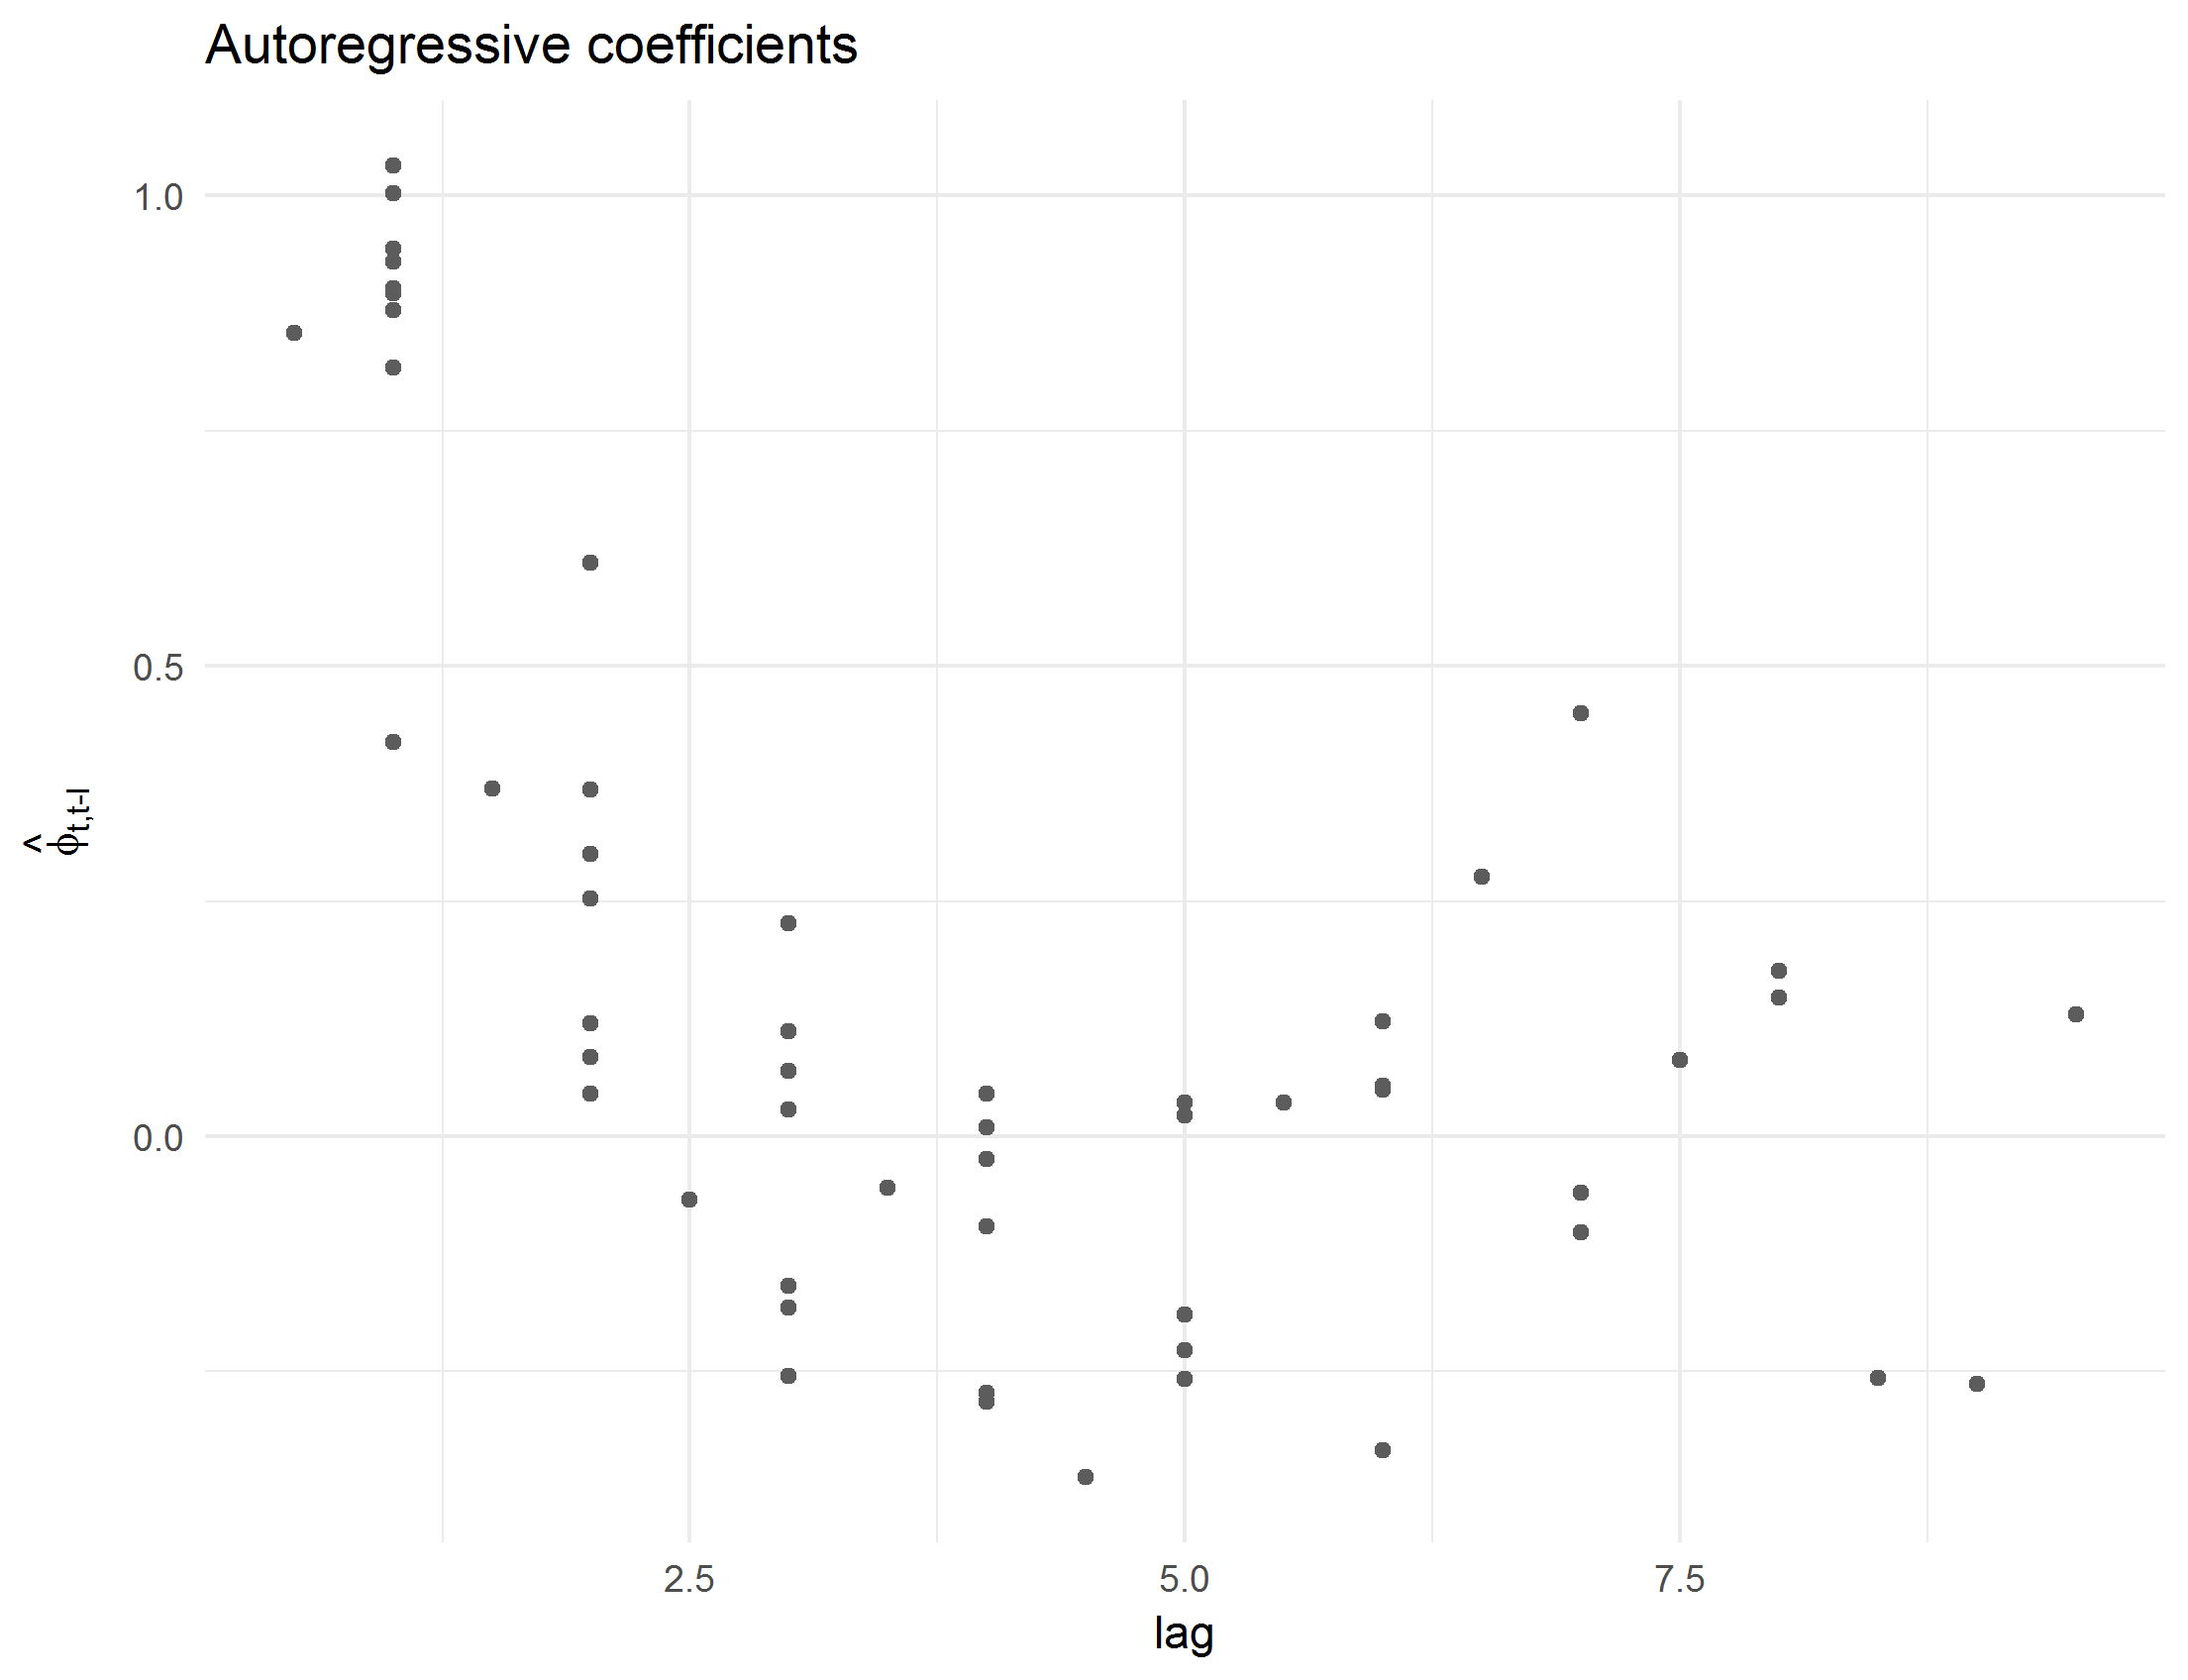
\includegraphics[width=0.65\textwidth]{img/cattle/cattleA-regressogram}}%\caption{\textit{Sample generalized autoregressive parameters $\hat{\phi}_{ts}$.}}
  \hfill
    \subfloat[\textit{Sample innovation variances $\hat{\sigma}_t^2$}]{\label{fig:cattleA-innovation-variogram} 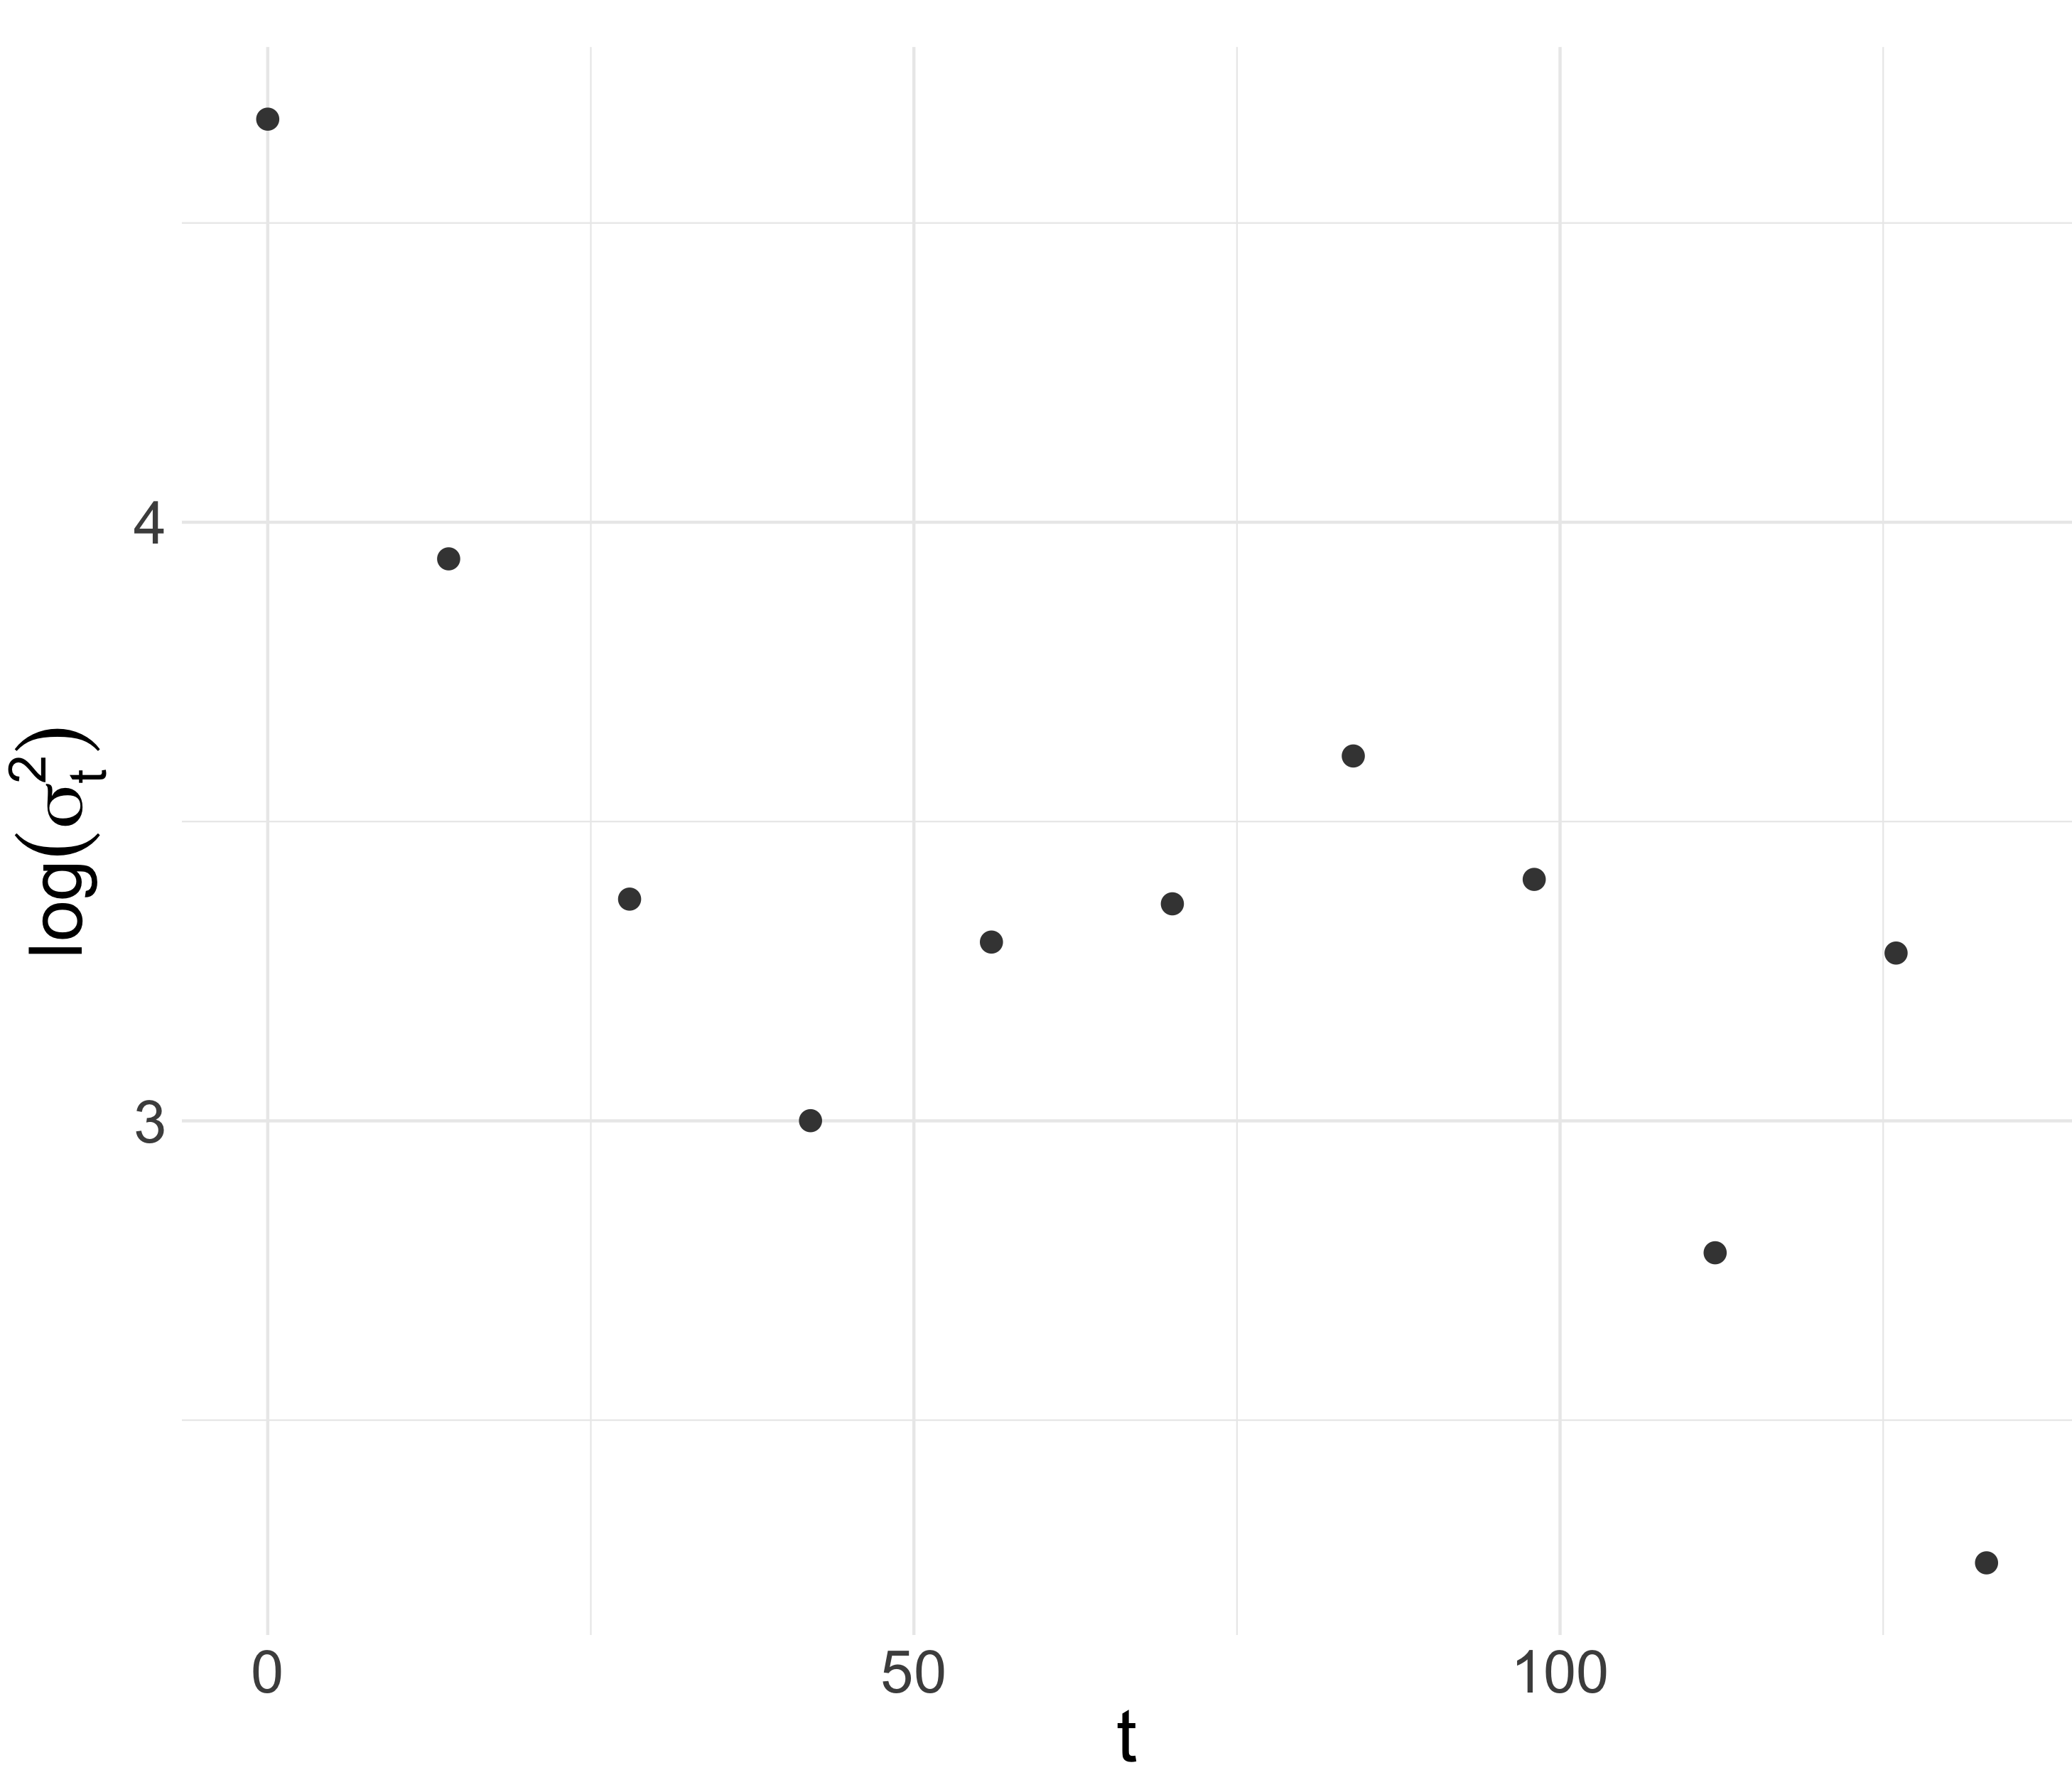
\includegraphics[width=0.65\textwidth]{img/cattle/cattleA-innovation-variogram}}%\caption{\textit{Sample innovation variances $\hat{\sigma}_t^2$}}
% \begin{subfigure}[t]{.65\textwidth}
%  \centering
%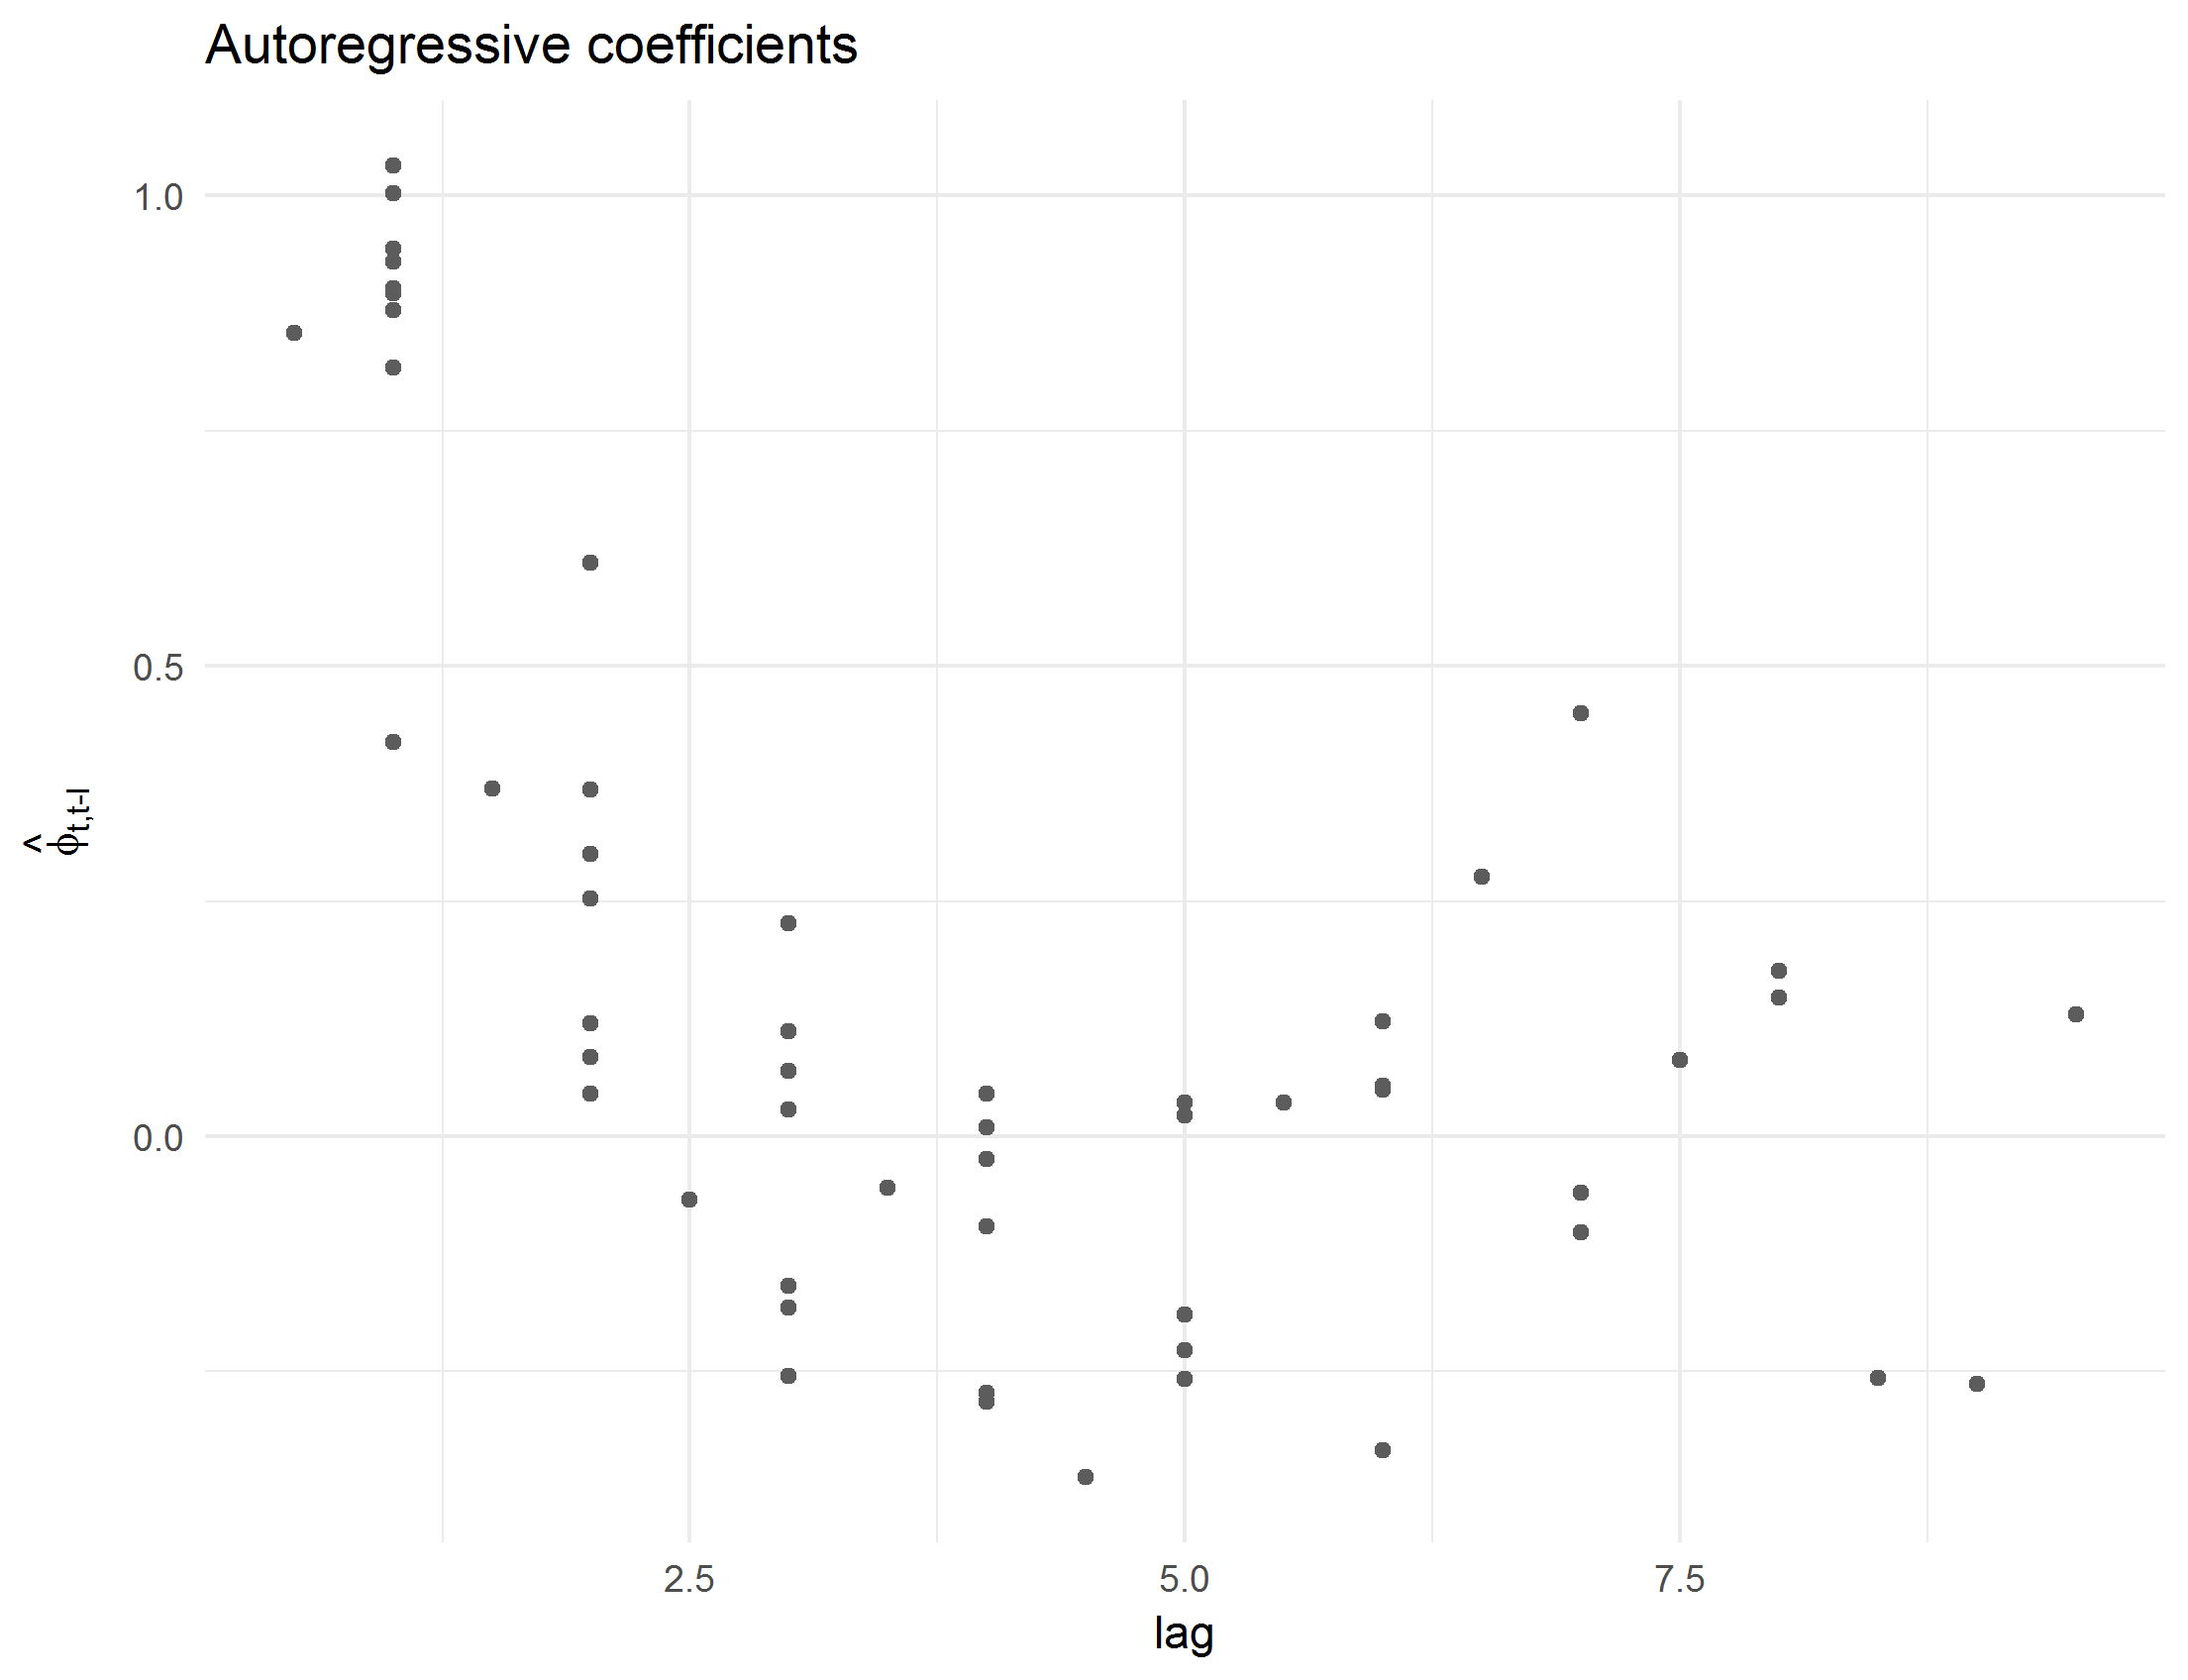
\includegraphics[width = \textwidth]{img/cattle/cattleA-regressogram}
% \caption{\textit{Sample generalized autoregressive parameters $\hat{\phi}_{ts}$.}}
%\label{fig:cattleA-regressogram}
% \end{subfigure}
%   \centering
%    \begin{subfigure}[t]{.65\textwidth}
%    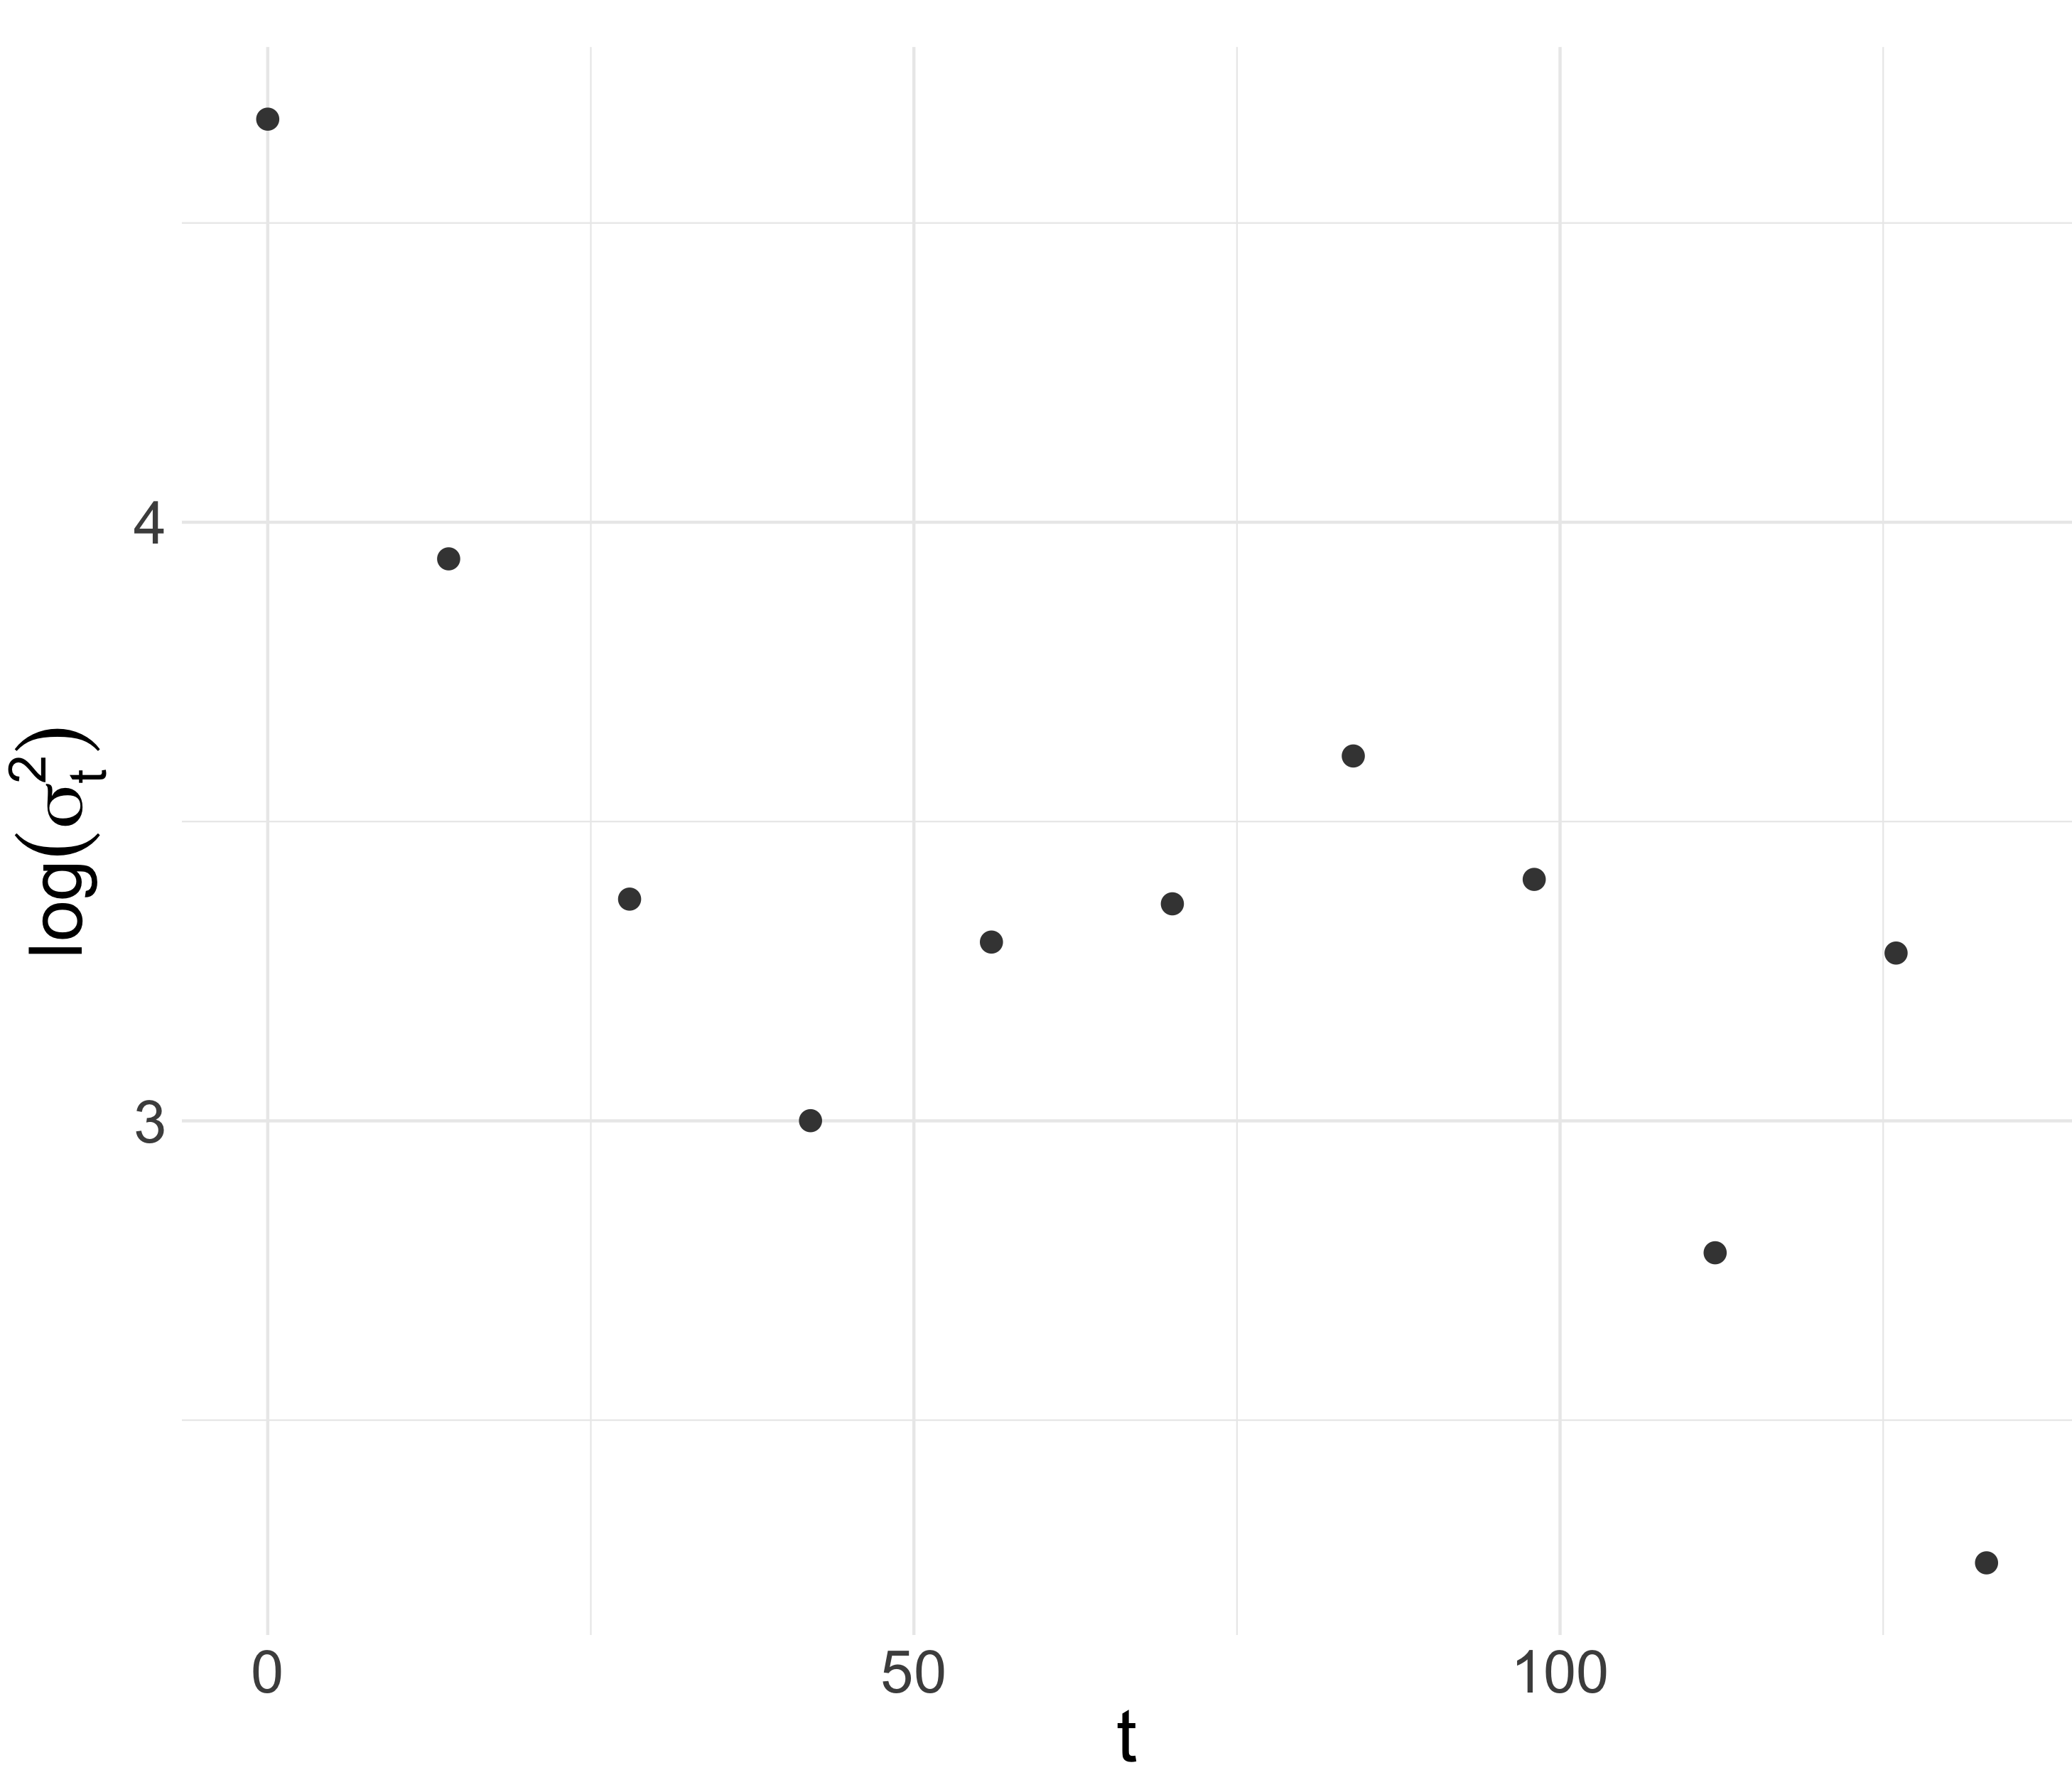
\includegraphics[width=\textwidth]{img/cattle/cattleA-innovation-variogram}
% \caption{\textit{Sample innovation variances $\hat{\sigma}_t^2$}} \label{fig:cattleA-innovation-variogram}
% \end{subfigure}
 \caption{\textit{Empirical estimates of the parameters of the Cholesky decomposition of the sample covariance matrix.}} \label{fig:cattleA-innovation-variogram-and-regressogram}
\end{center}
\end{figure}

%
%\begin{figure}[H] \label{fig:cattleA-innovation-variogram}
%\begin{center}
%    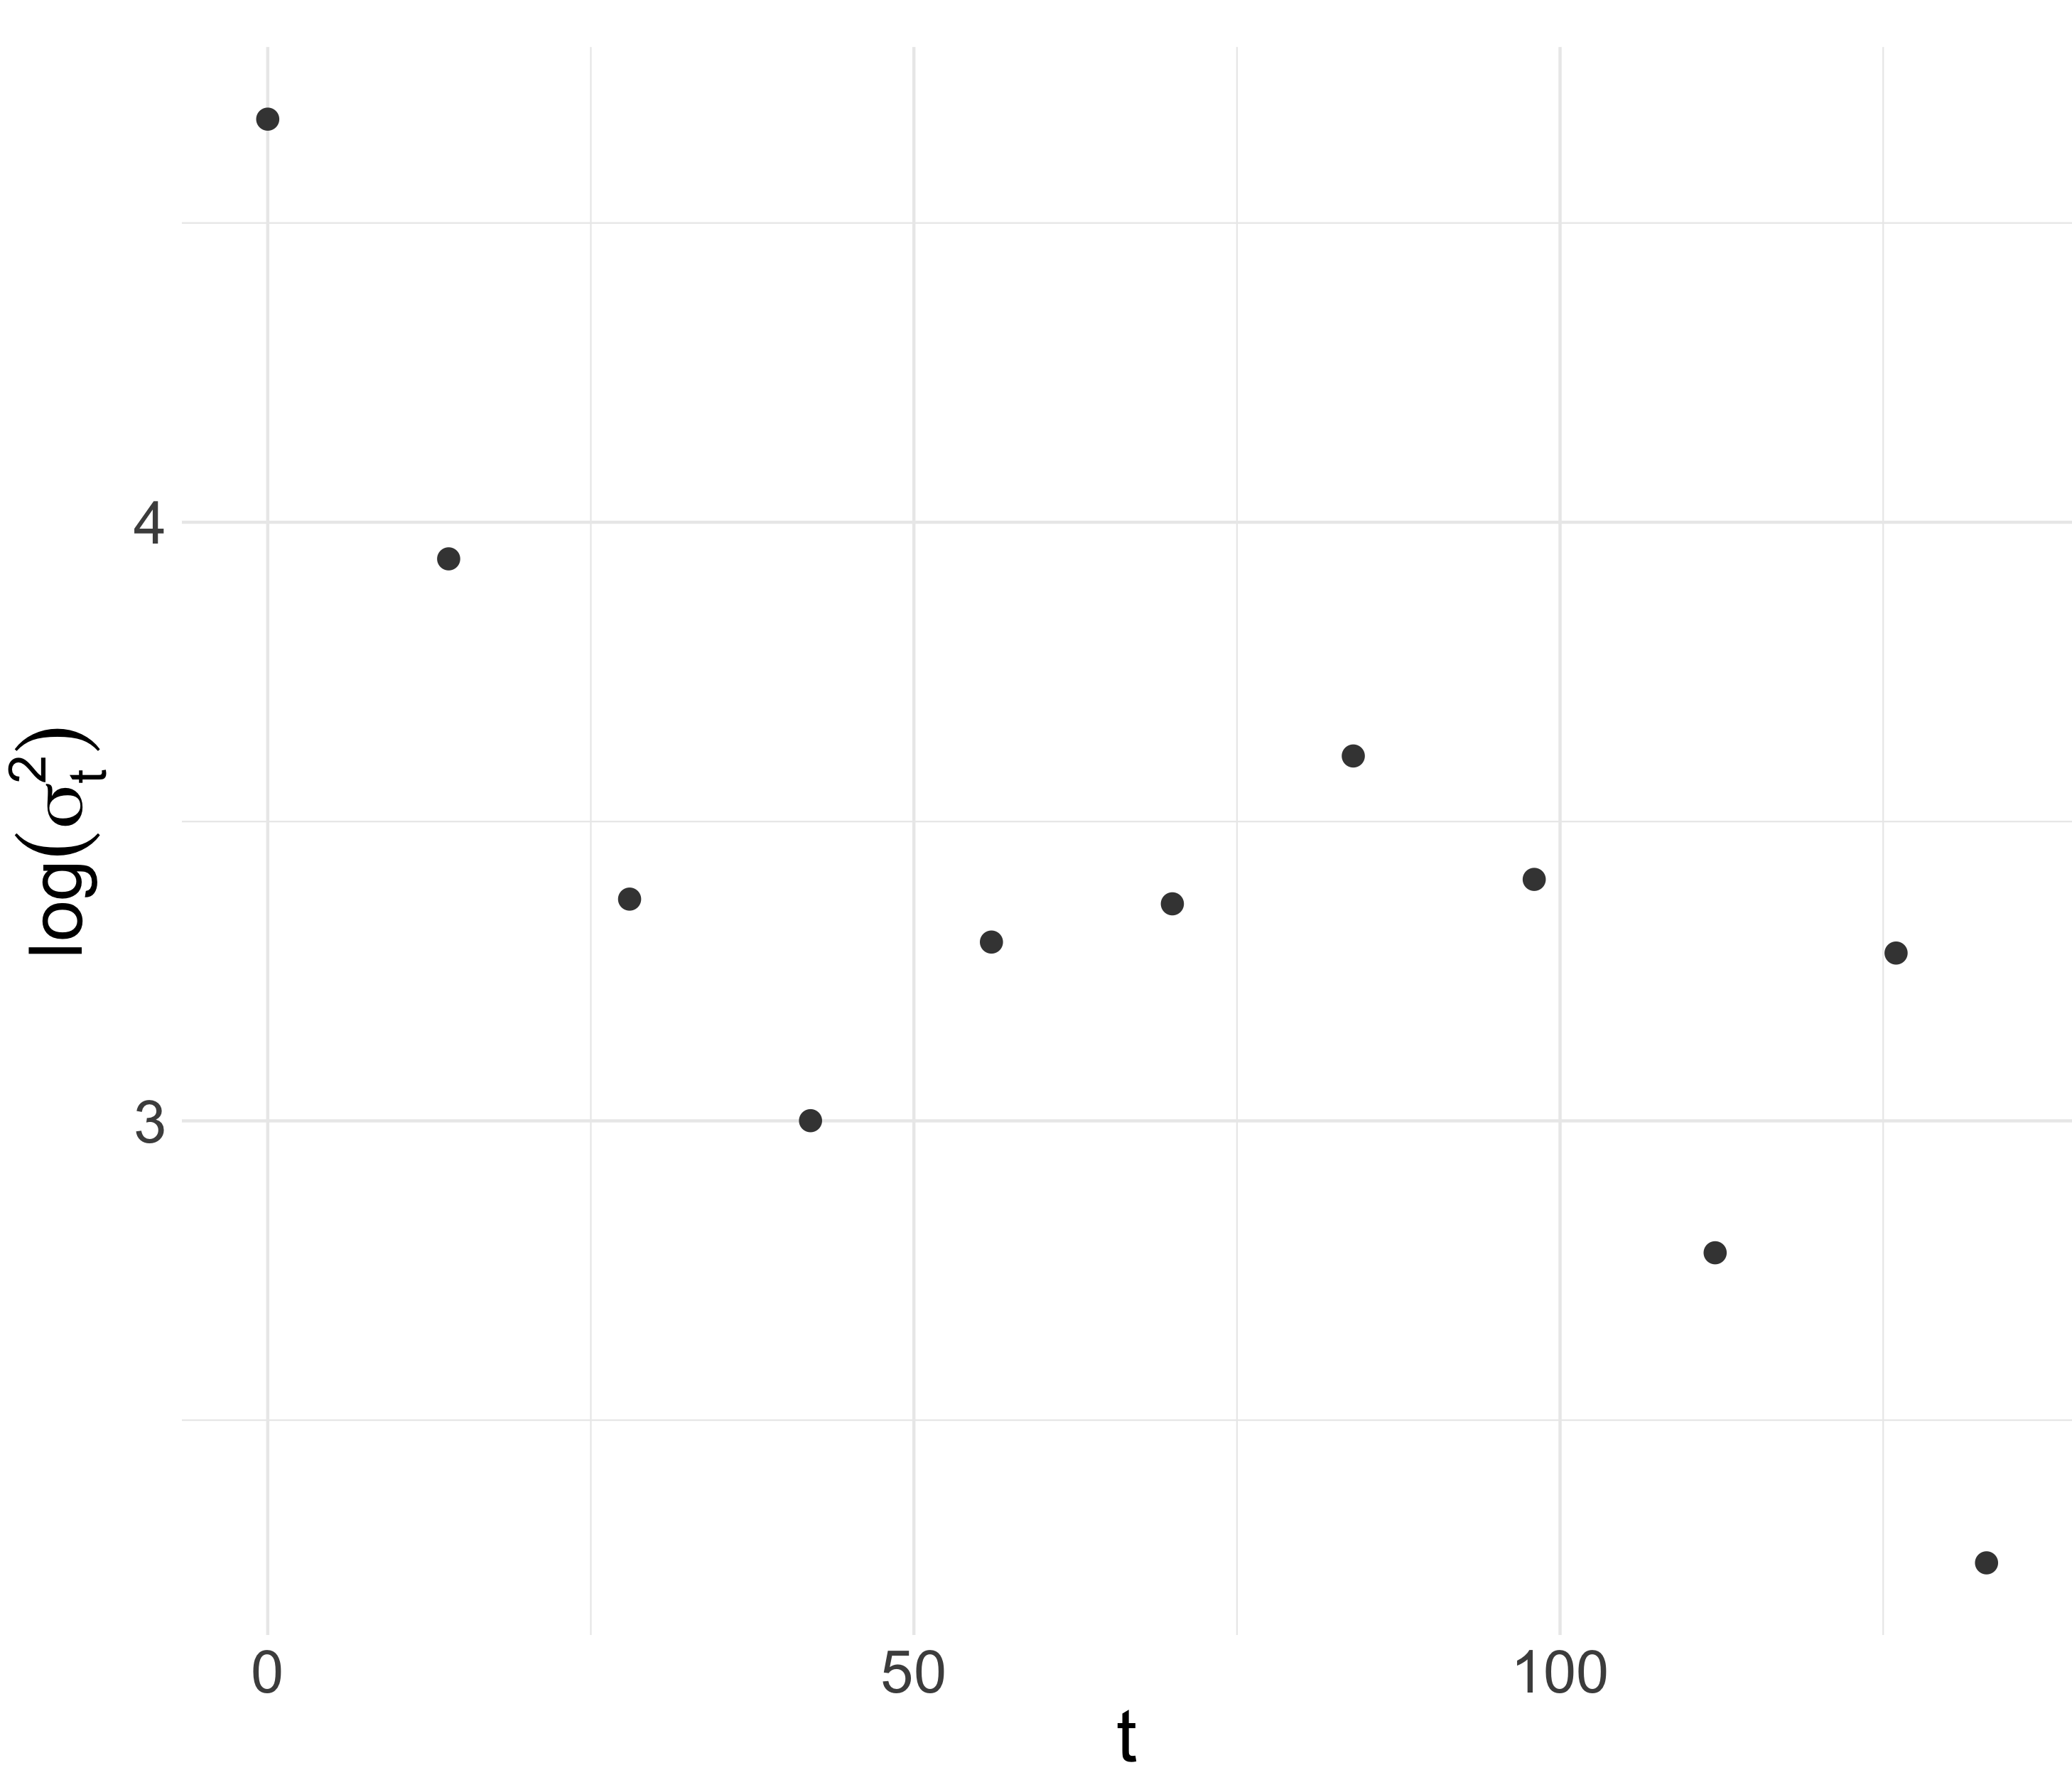
\includegraphics[width=\textwidth]{img/cattle/cattleA-innovation-variogram}
%\end{center}
% \caption{Sample estimates of innovation variances $\sigma_t^2$ obtained by applying the modified Cholesky decomposition to the sample covariance matrix.}
% \end{figure}
%
%\begin{figure}[H] \label{fig:cattleA-regressogram}
%\begin{center}
%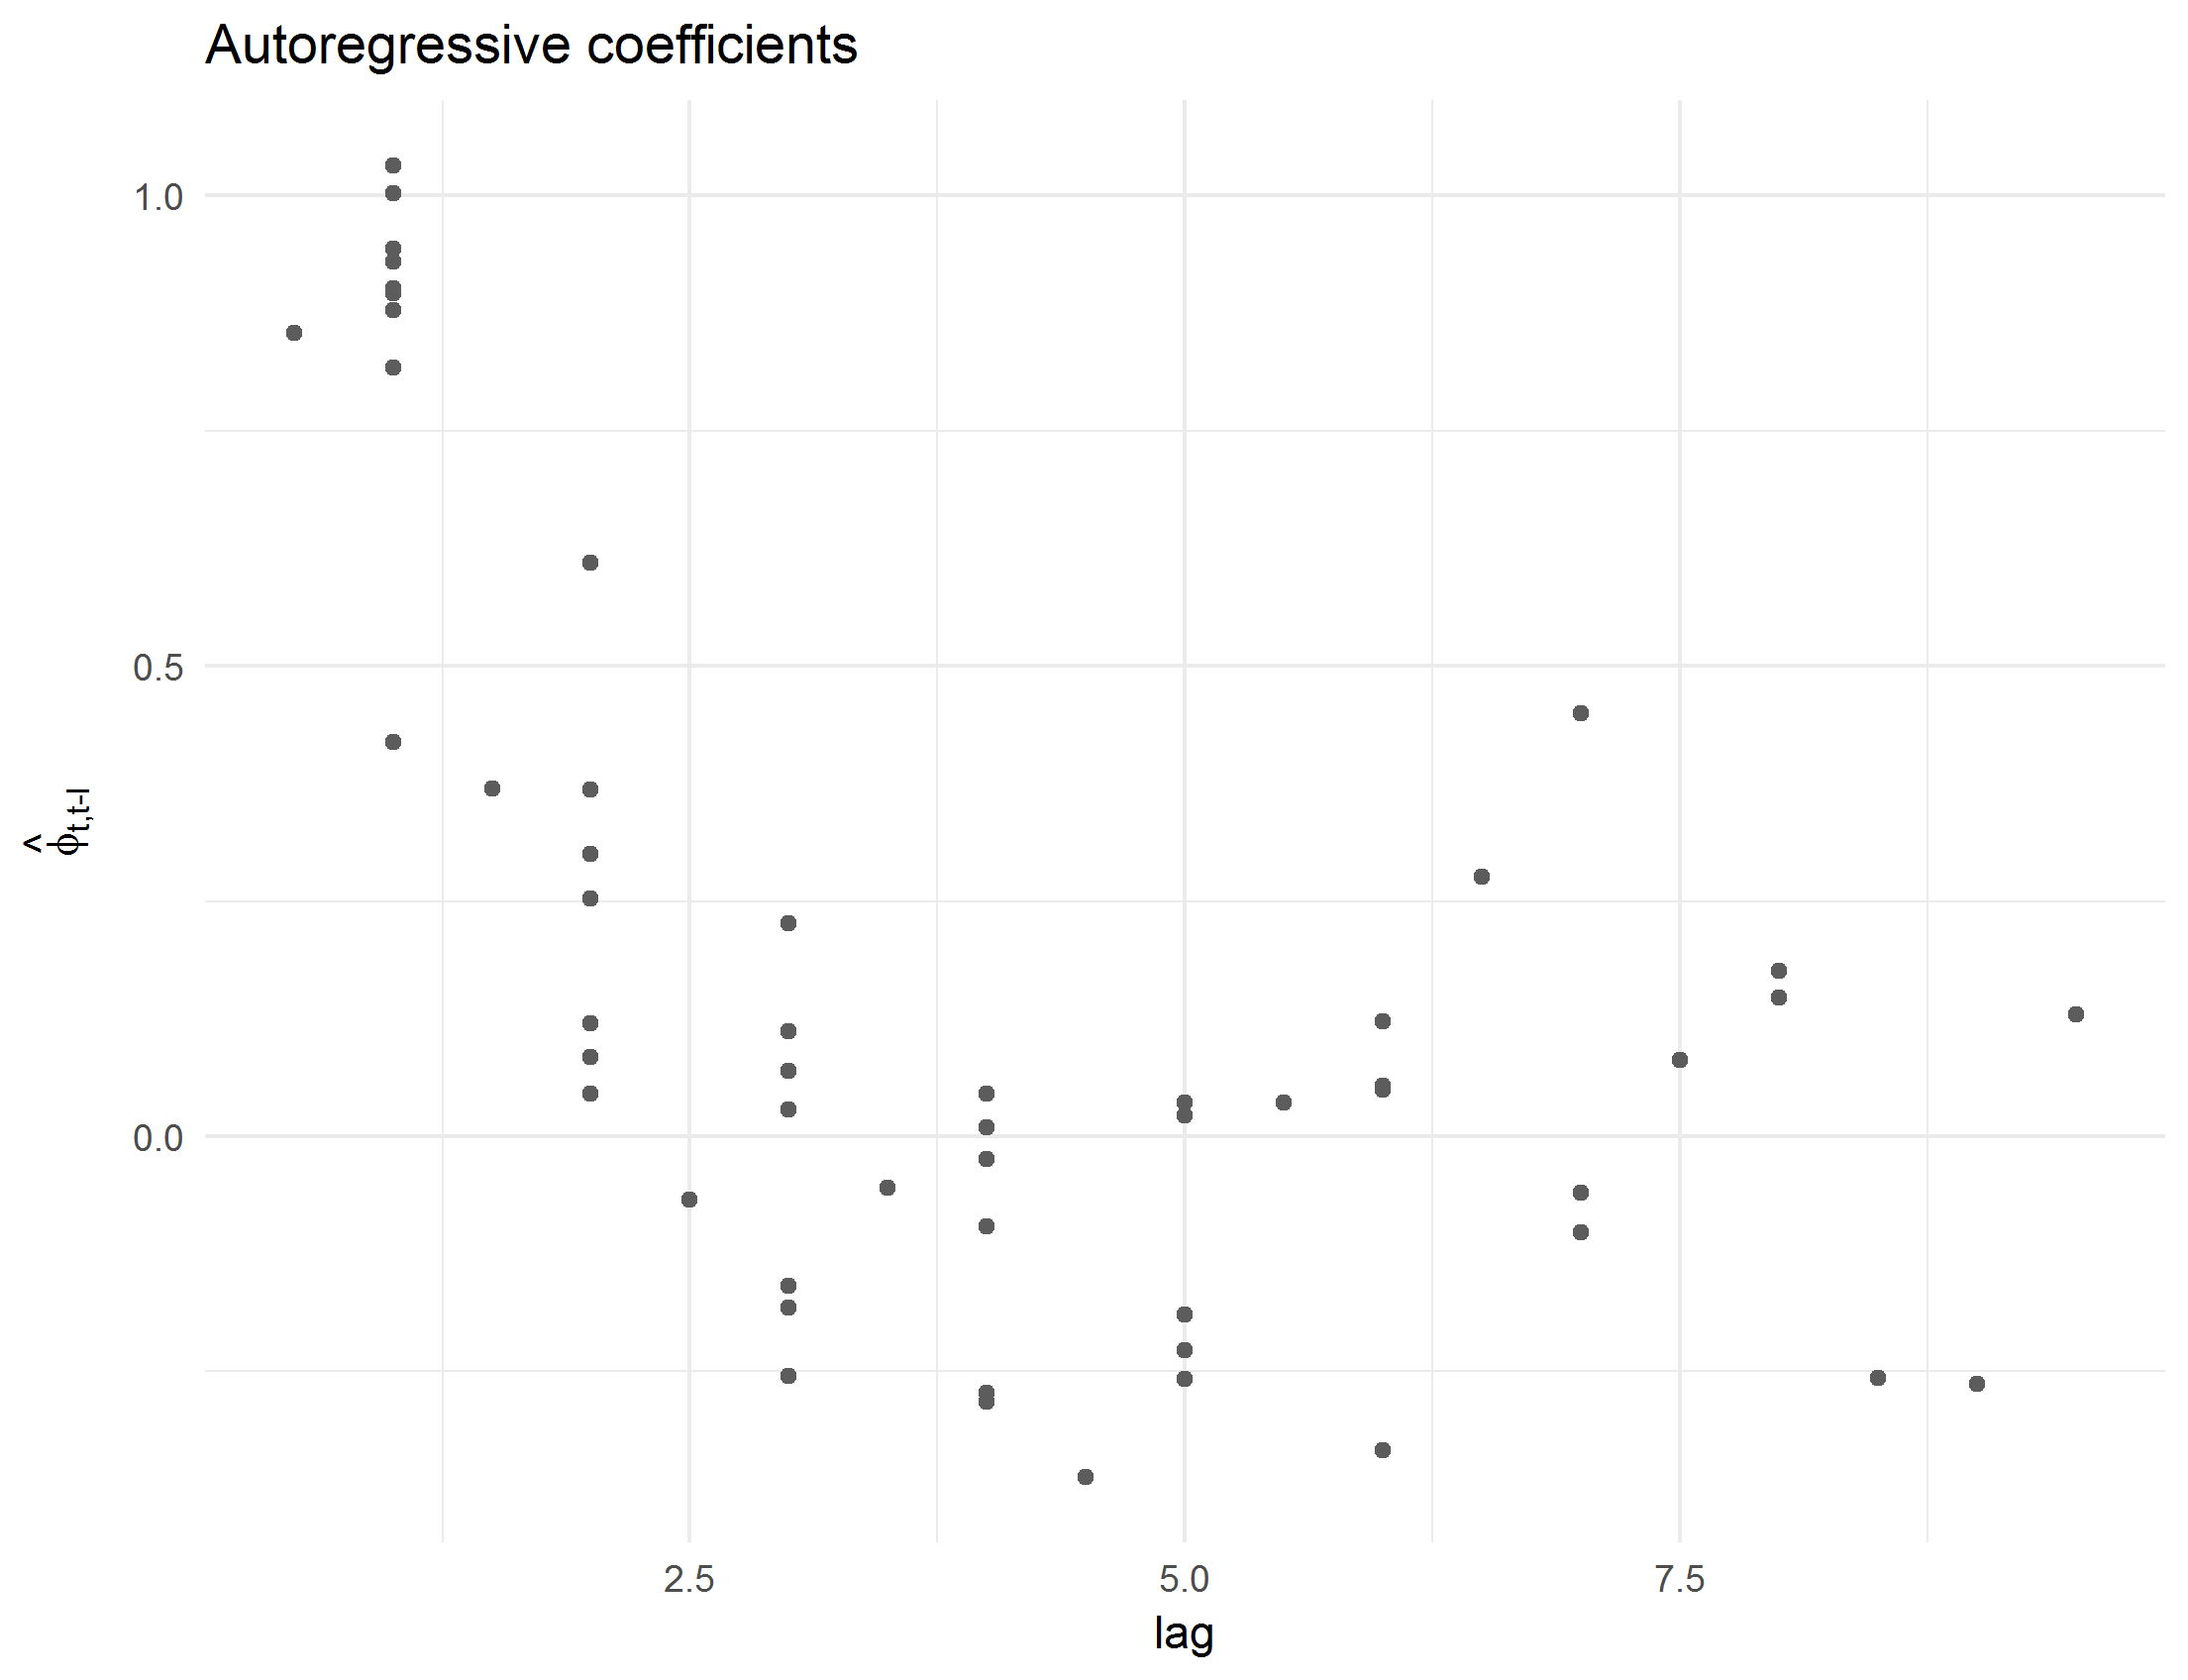
\includegraphics[width = \textwidth]{img/cattle/cattleA-regressogram}
%\end{center}
% \caption{Sample estimates of the generalized autoregressive parameters $\phi_{ij}$ obtained by applying the modified Cholesky decomposition to the sample covariance matrix.}
%\end{figure} 

Analyzing the sample regressogram (Figure~\ref{fig:cattleA-regressogram}) and sample innovation variogram (Figure~\ref{fig:cattleA-innovation-variogram}), \cite{pourahmadi1999joint} suggested that both sample generalized autoregressive parameters and the logarithms of the innovation variances can be characterized in terms of cubic functions of the lag only. They model 
\begin{align}
\begin{split} \label{eq:pourahmadi-cubic-model}
\phi_{ts} = x'_{ts}\beta, \\
\log\left(\sigma_t^2\right) = z'_{t}\gamma, 
\end{split}
\end{align}
\noindent
for $t = t_2,\dots, t_{11}$ where 
\begin{align*}
x'_{ts} = \begin{bmatrix} 1 & t - s& \left(t - s\right)^2 & \left(t - s\right)^3 \end{bmatrix},\; \mbox{and } z'_{t} = \begin{bmatrix} 1 & t& t^2& t^3 \end{bmatrix}.
\end{align*}
\noindent
They estimate $\beta$ and $\gamma$ via maximum likelihood.  Figure~\ref{fig:cattleA-smoothed-regressogram-variogram} shows the estimated cubic polynomials corresponding to Model~\eqref{eq:pourahmadi-cubic-model}. 

%\begin{figure}[H]
%  \centering
% \begin{subfigure}[t]{.65\textwidth}
%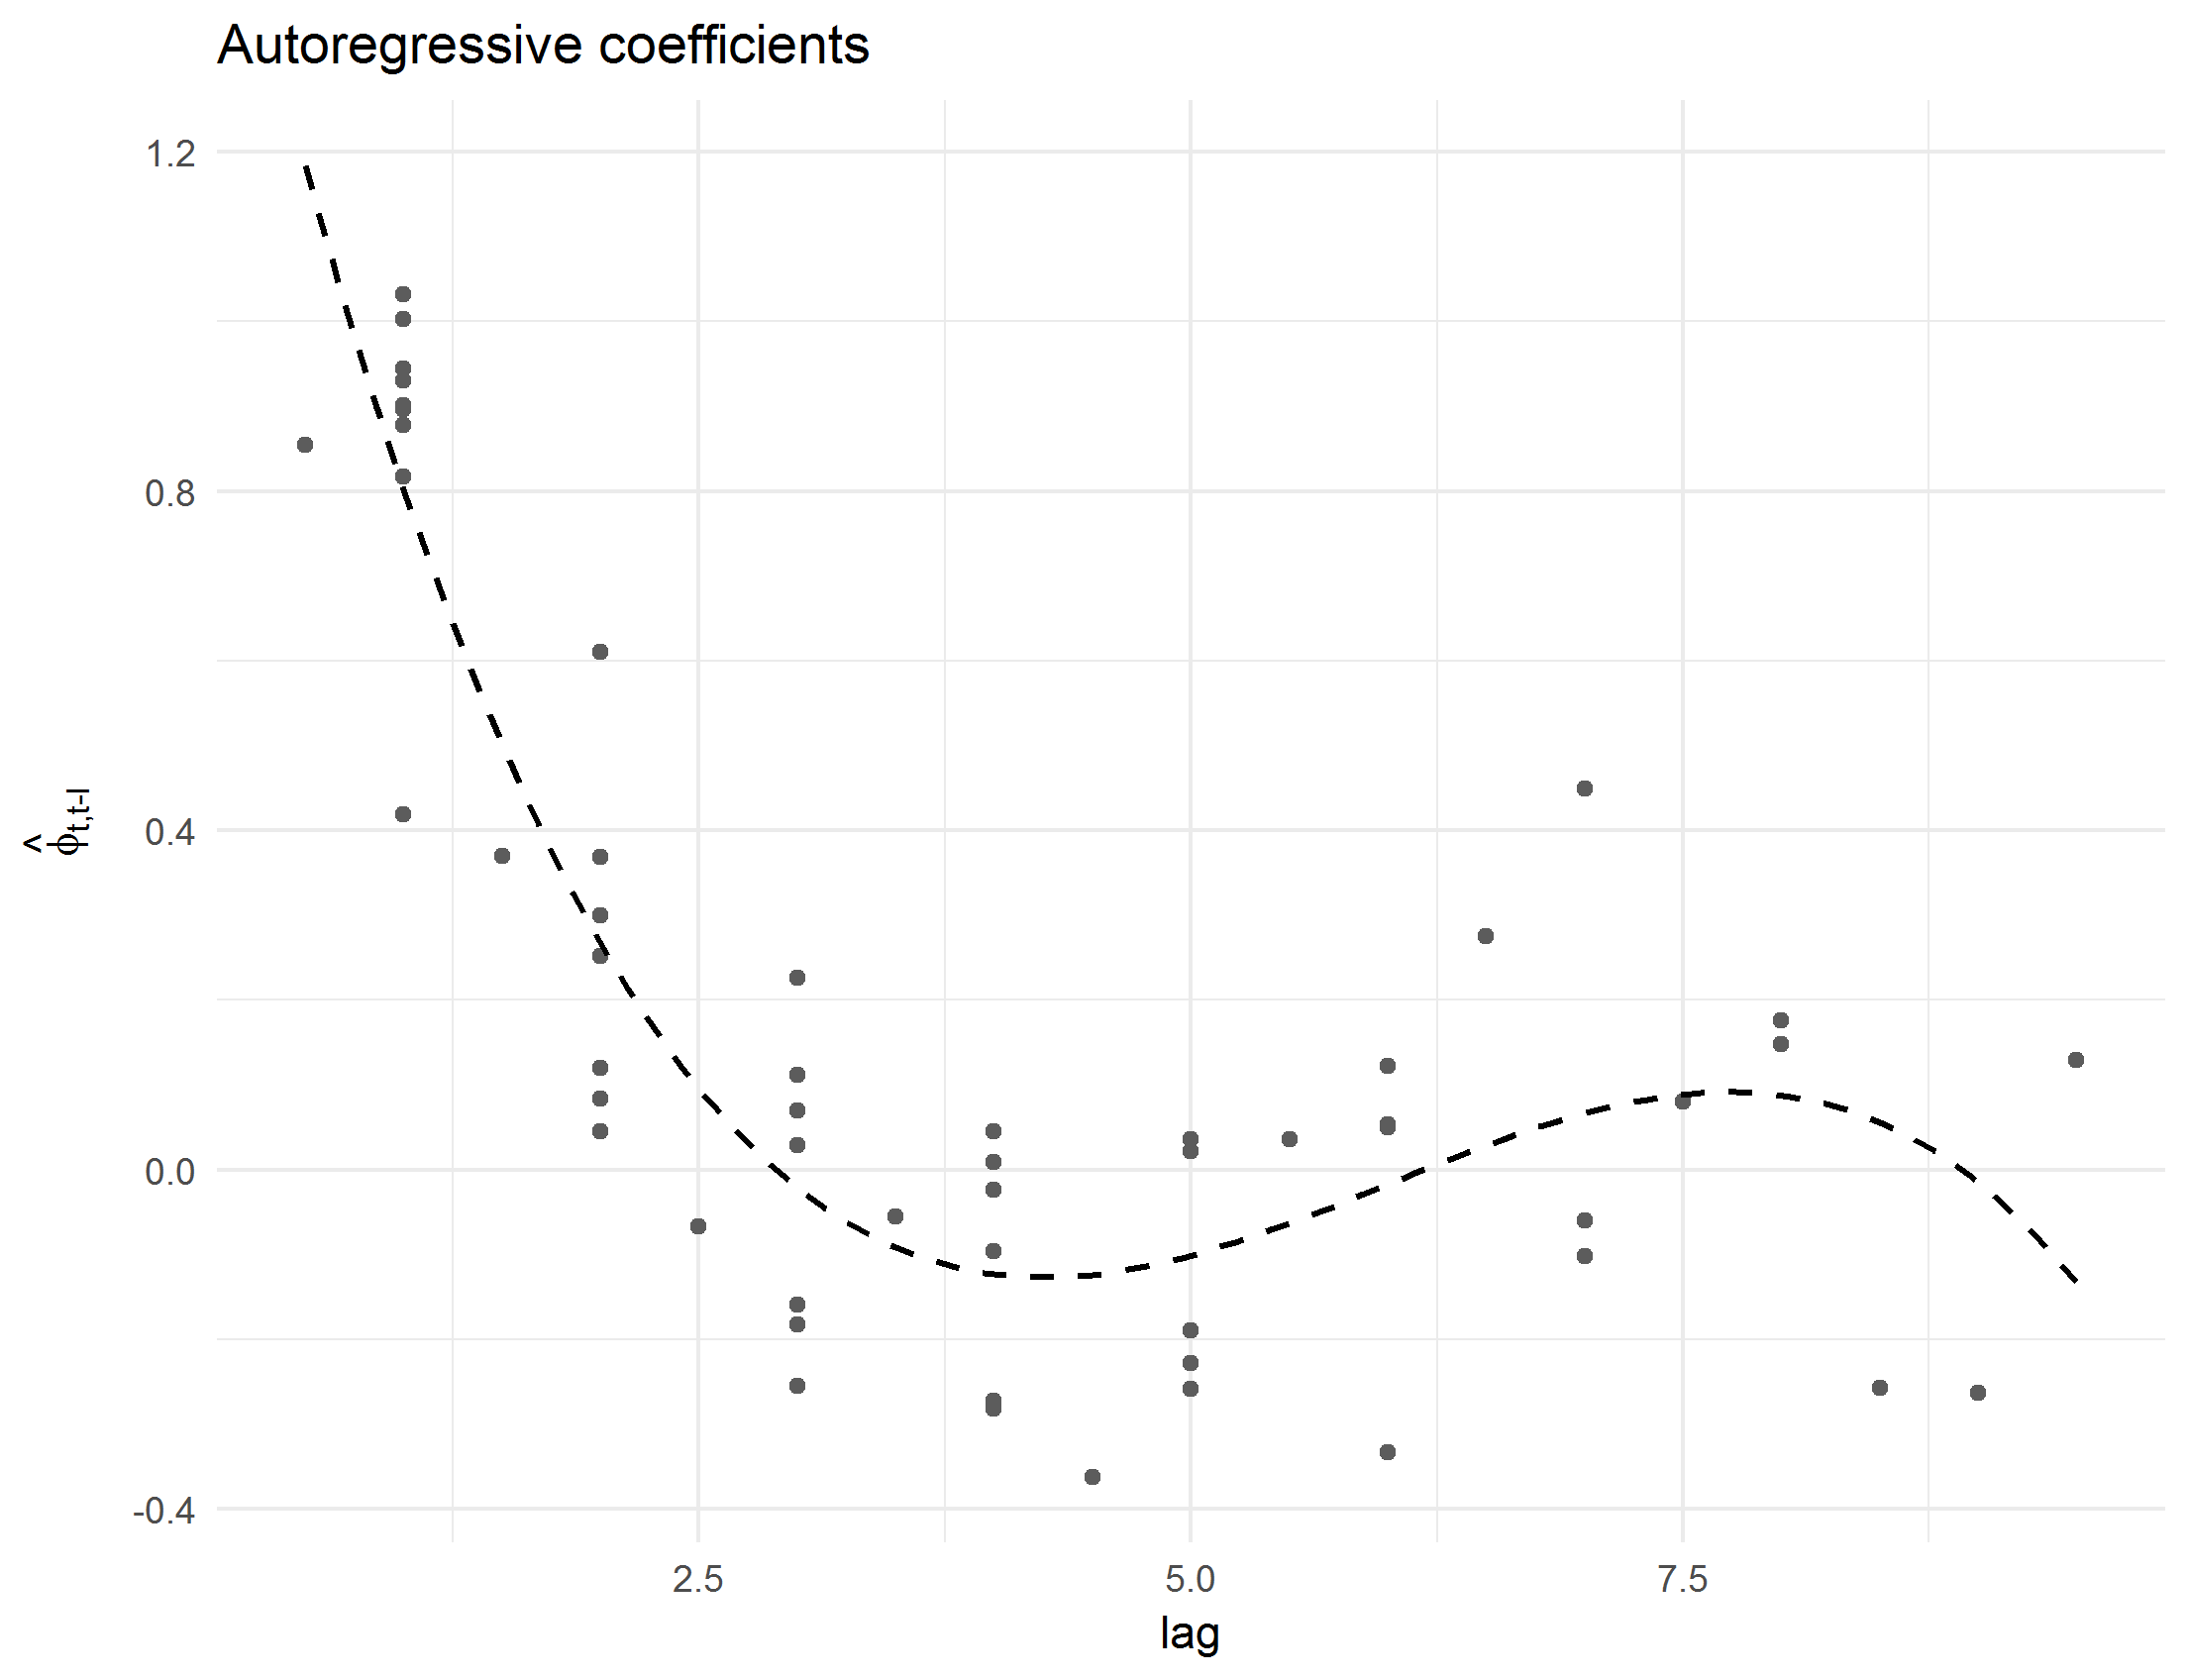
\includegraphics[width = \textwidth]{img/cattle/cattleA-regressogram-with-cubic-smooth}
% \caption{\textit{Smoothed sample regressogram.} }
% \label{fig:cattleA-innovariogram-with-cubic-smooth}
% \end{subfigure}
% \hfill
%   \centering
% \begin{subfigure}[t]{.65\textwidth}
%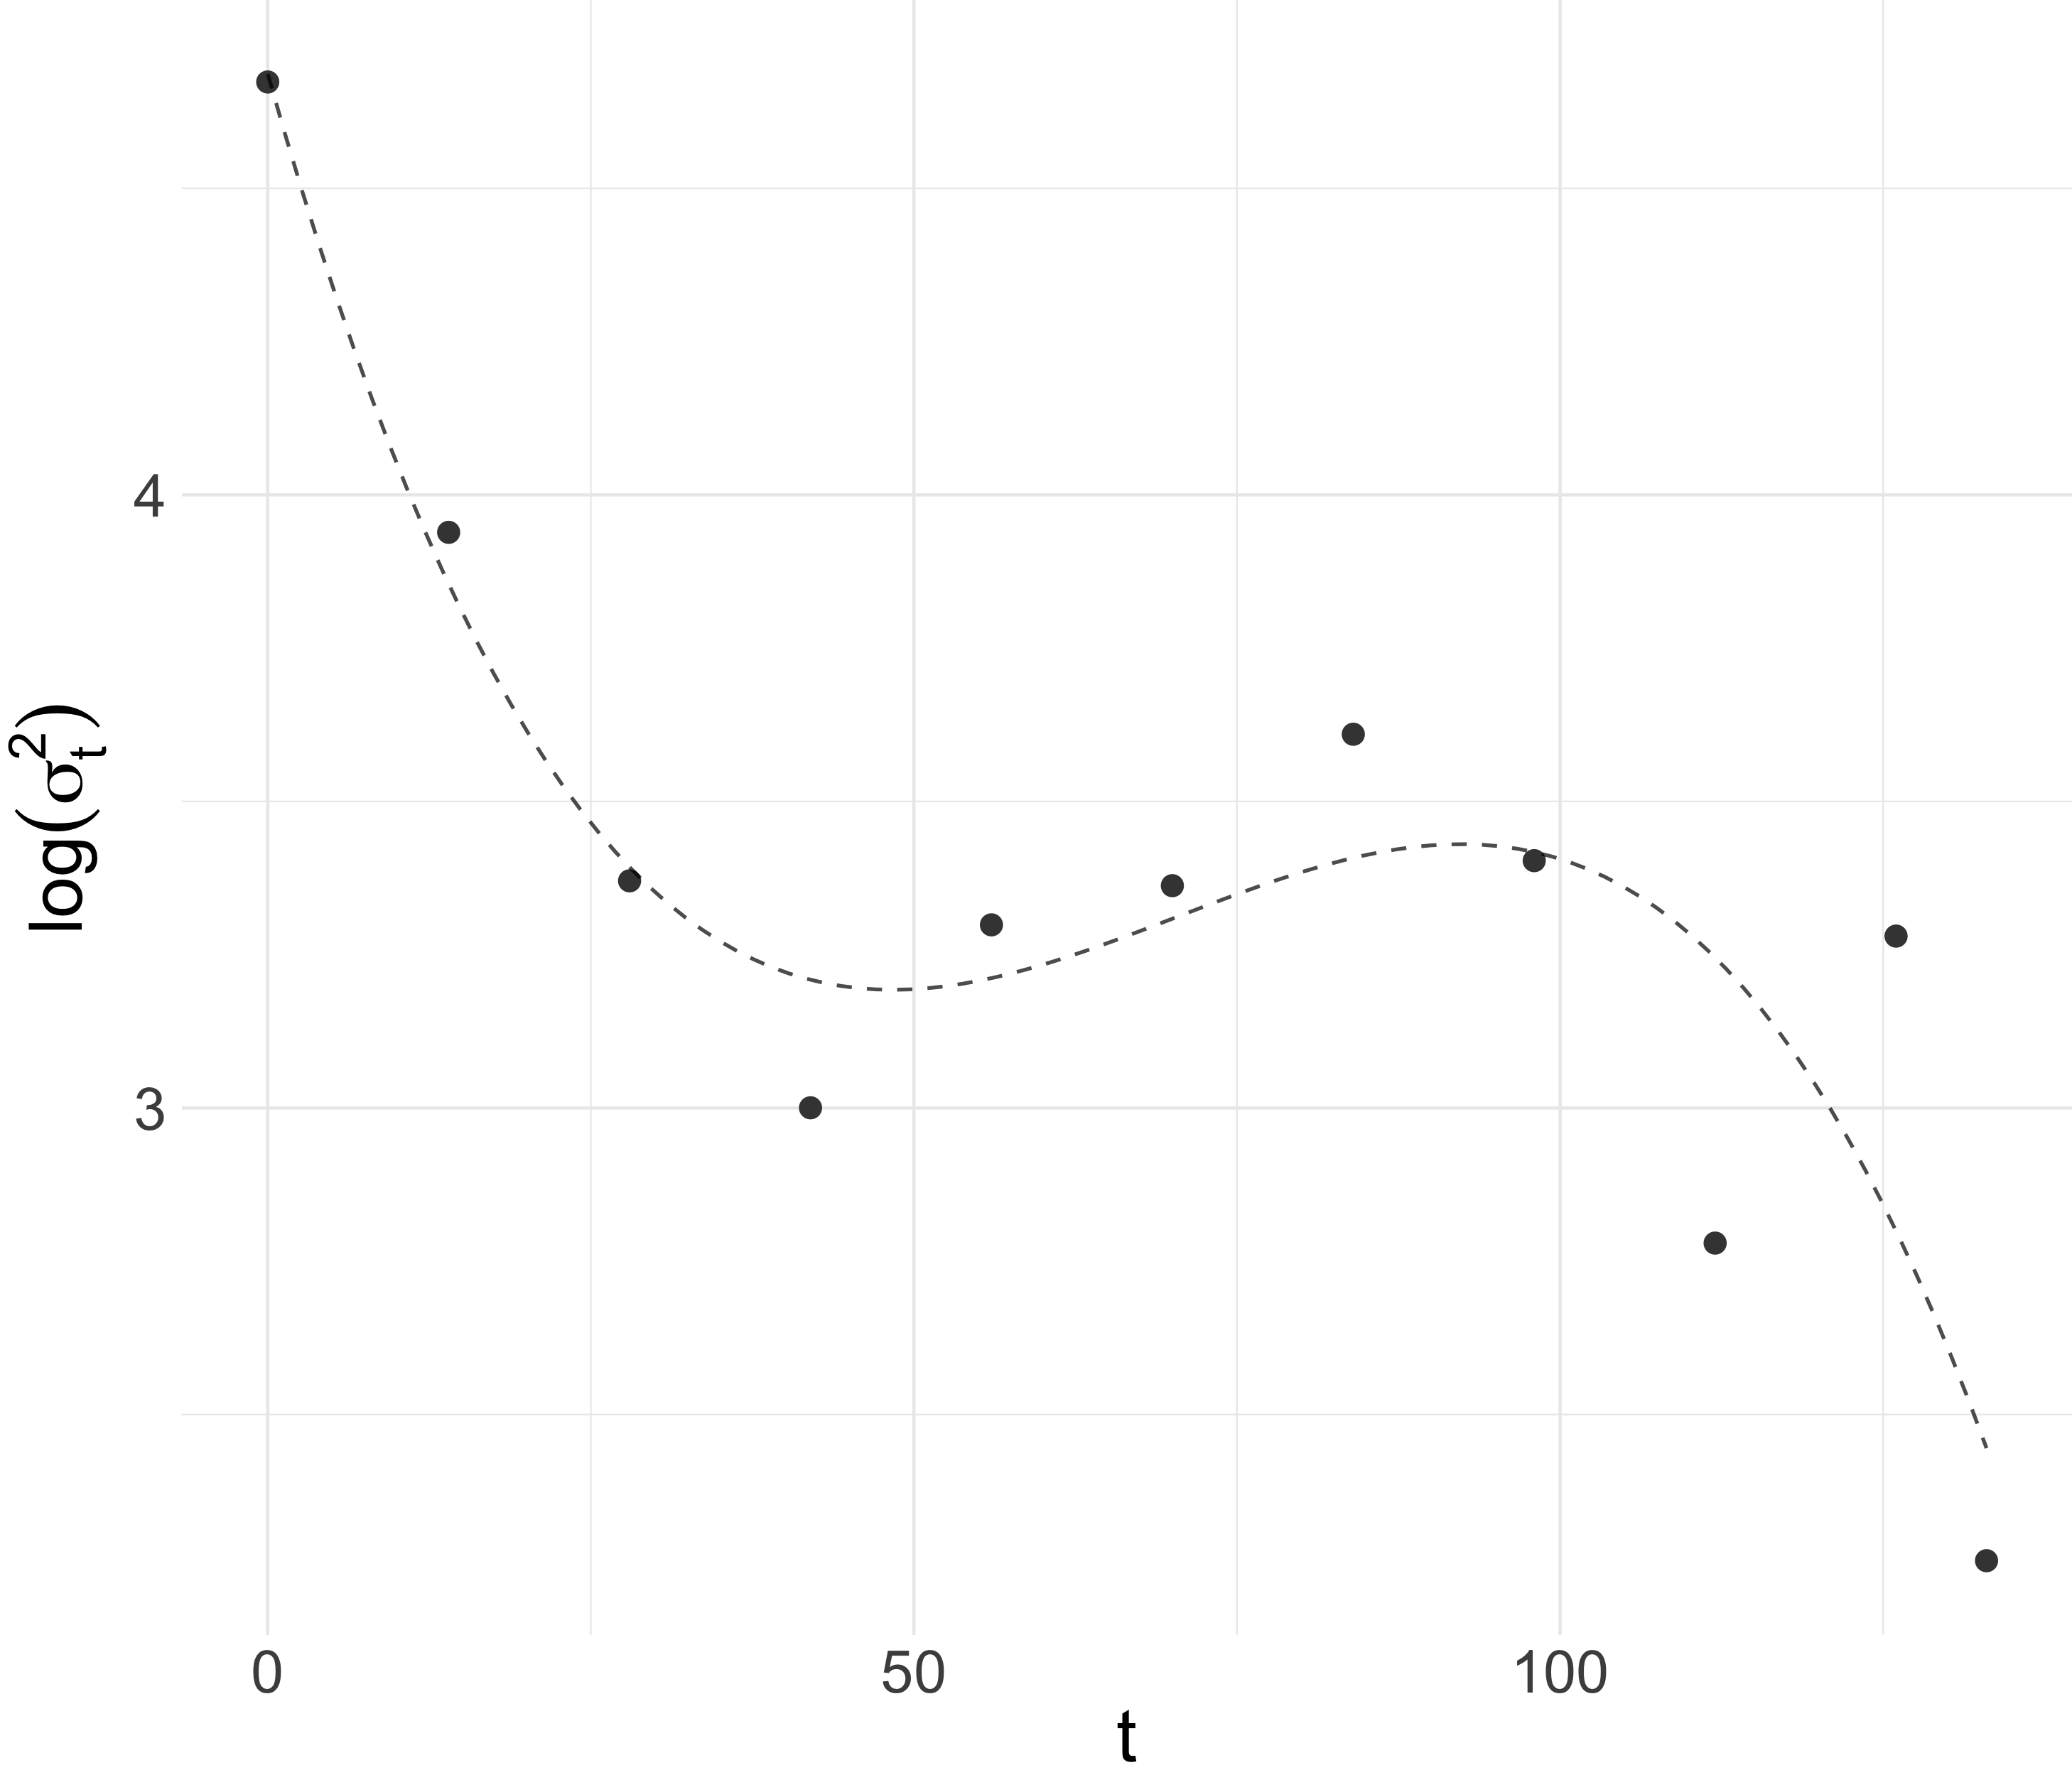
\includegraphics[width = \textwidth]{img/cattle/cattleA-innovariogram-with-cubic-smooth}
% \caption{\textit{Smoothed sample log innovation variances.} }
%\label{fig:cattleA-innovariogram-with-cubic-smooth}
% \end{subfigure}
 \begin{figure}[H]
\begin{center}
  \subfloat[\textit{Smoothed sample regressogram.}] {\label{fig:cattleA-regressogram-with-cubic-smooth} 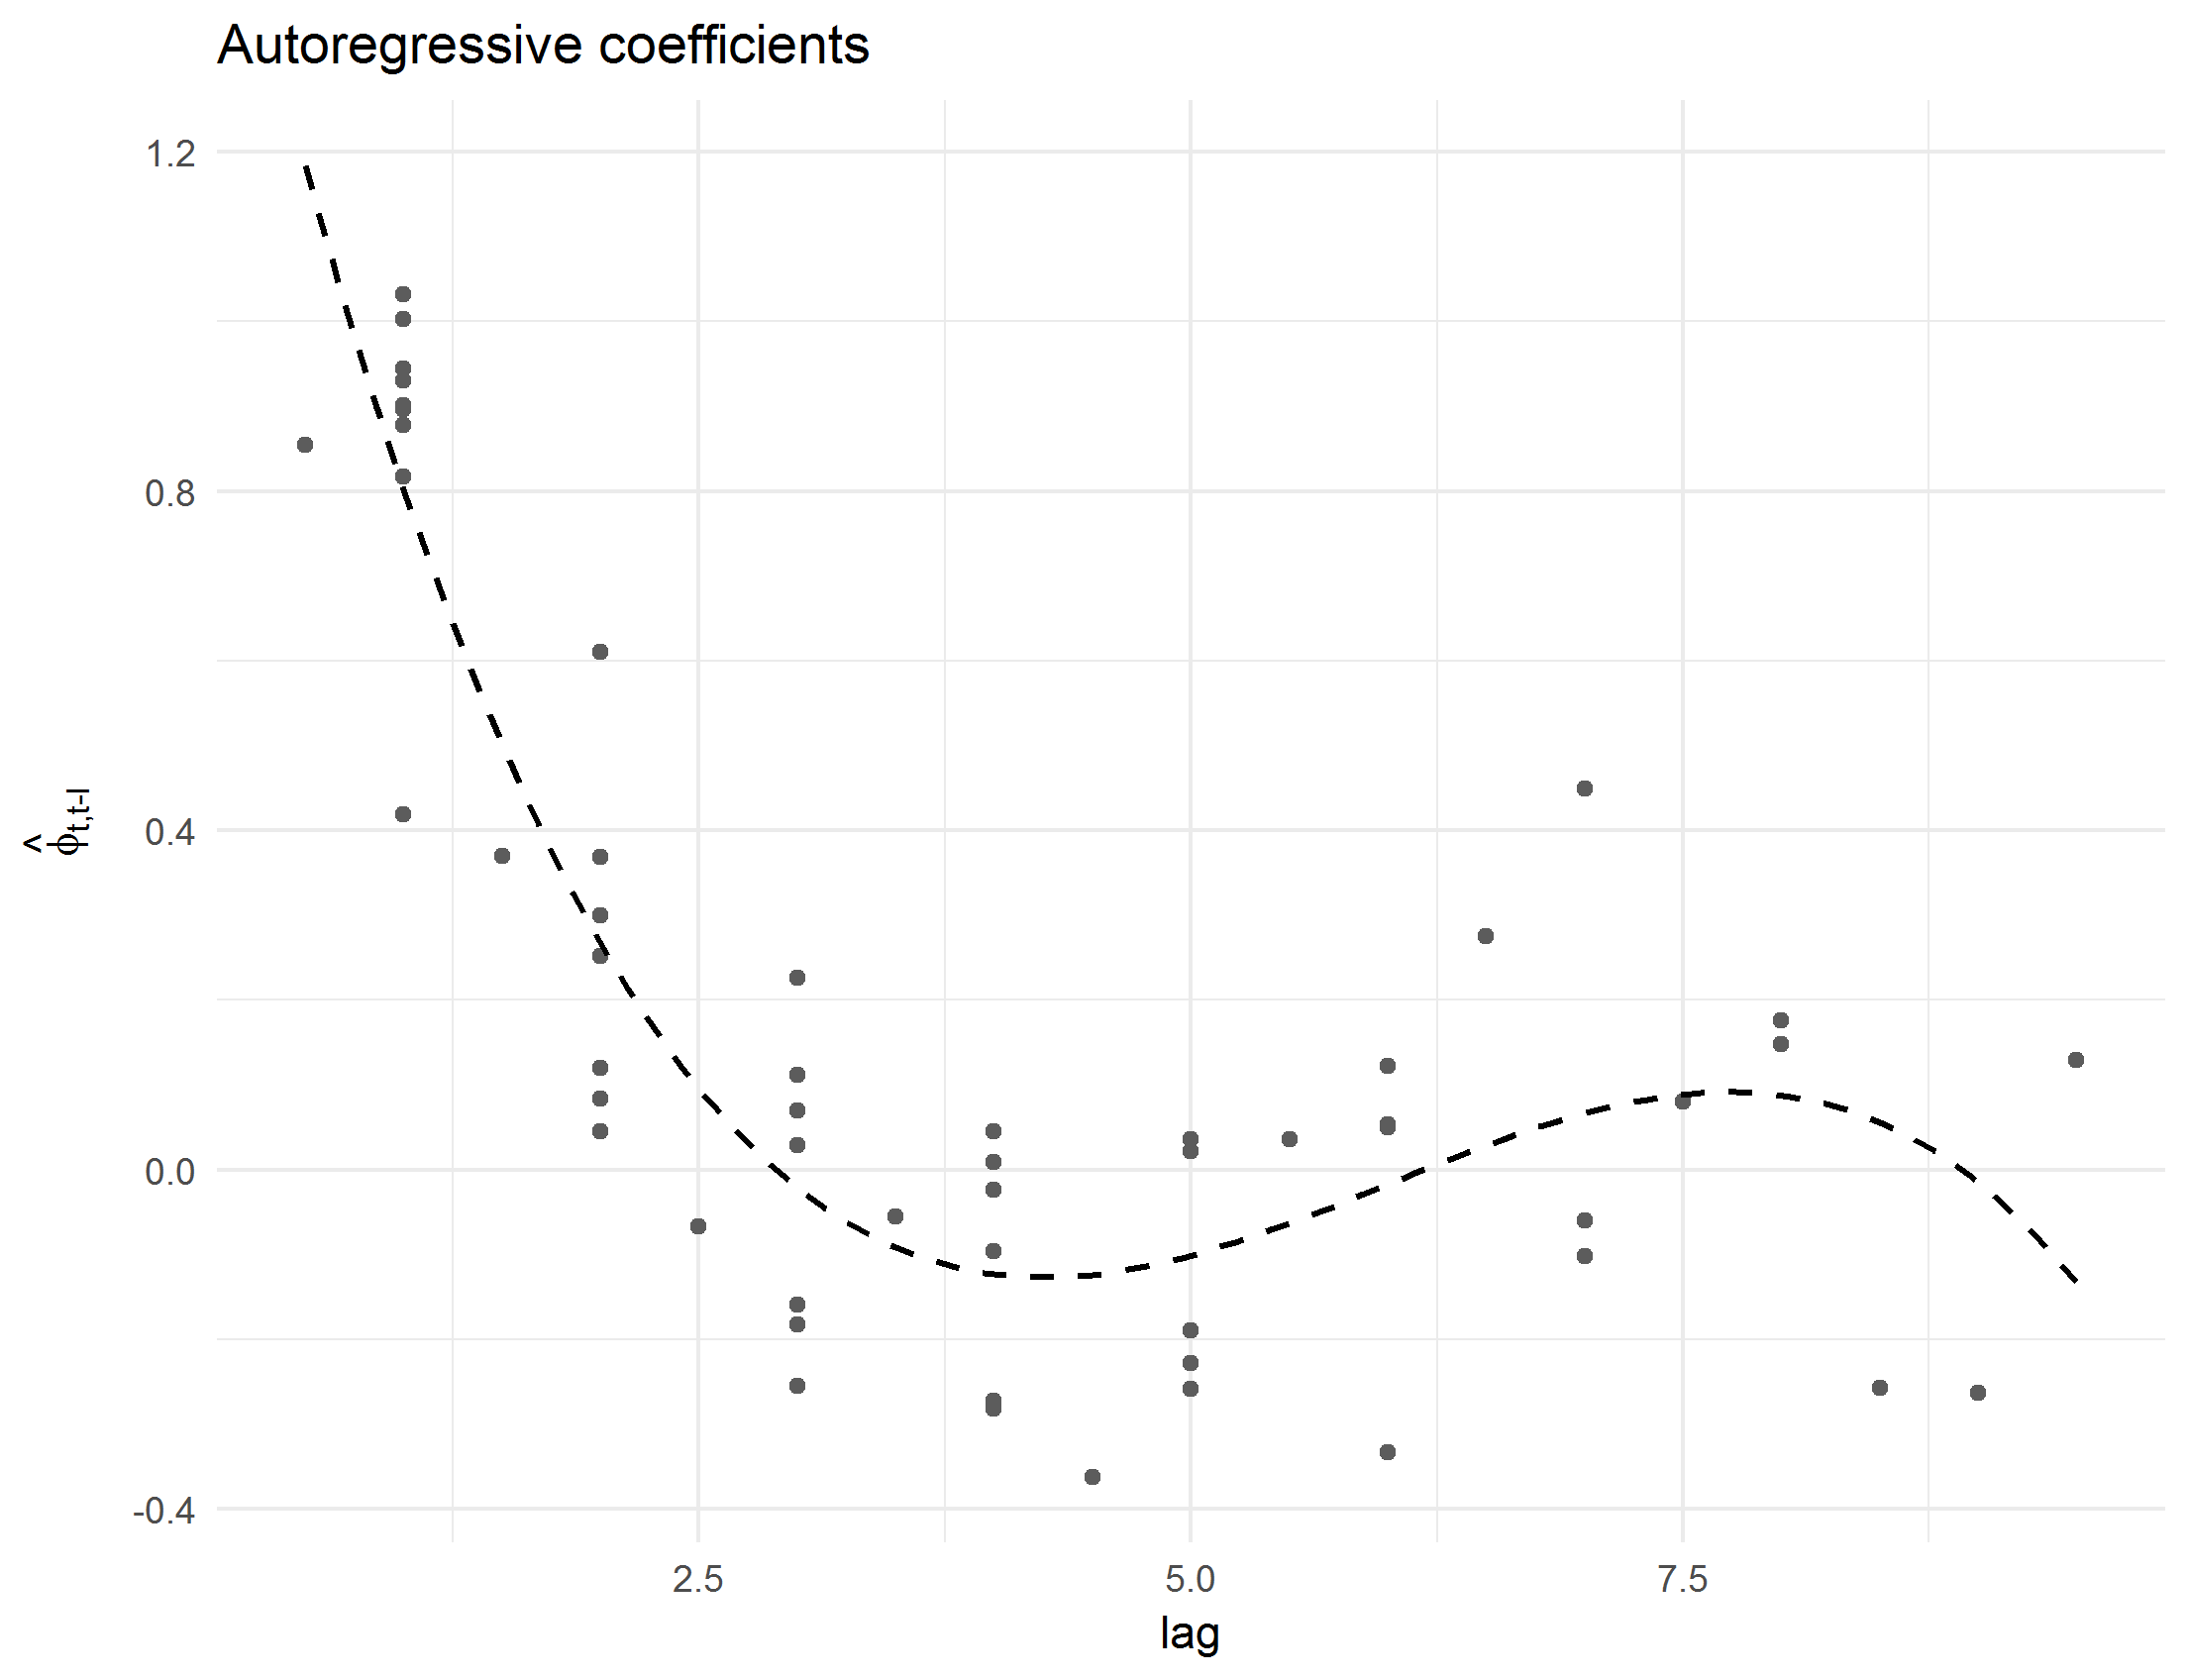
\includegraphics[width=0.65\textwidth]{img/cattle/cattleA-regressogram-with-cubic-smooth}}%\caption{\textit{Smoothed sample regressogram.}}
  \hfill
    \subfloat[\textit{Smoothed sample log innovation variances.}]{\label{fig:cattleA-innovariogram-with-cubic-smooth} 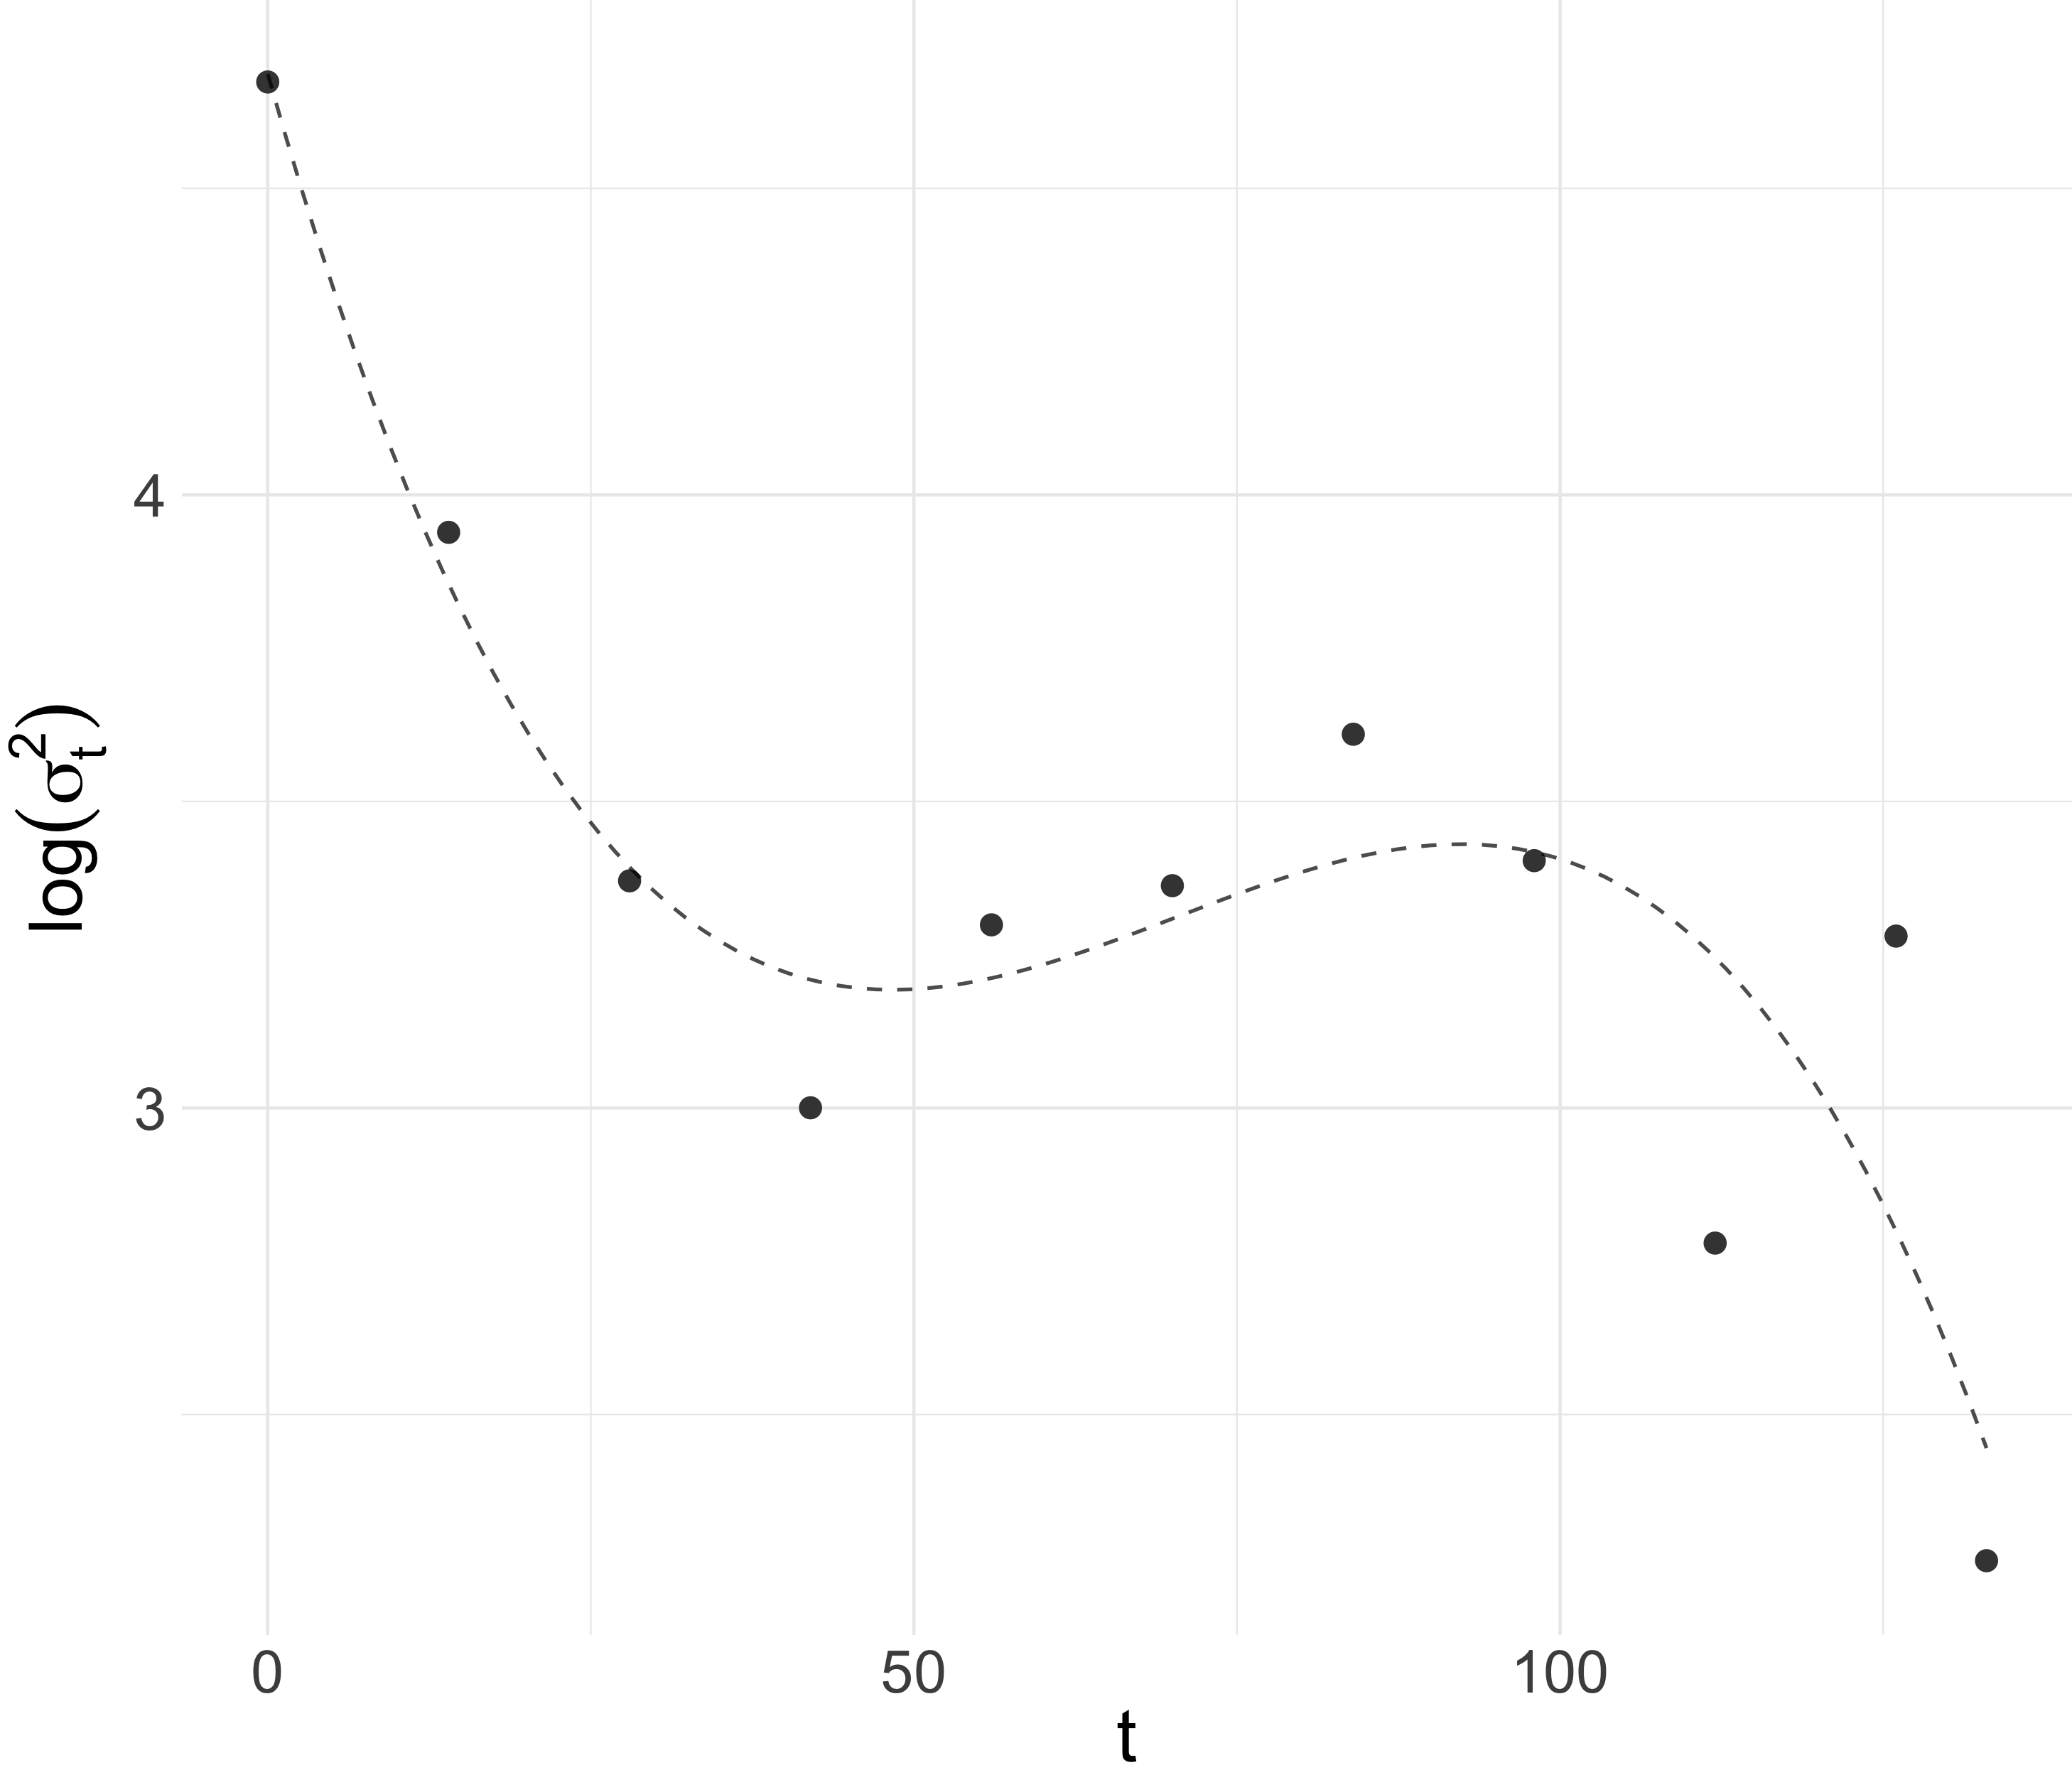
\includegraphics[width=0.65\textwidth]{img/cattle/cattleA-innovariogram-with-cubic-smooth}}%\caption{\textit{Smoothed sample log innovation variances.}}
 \caption{\textit{Cubic polynomomials fitted to the sample regressogram and log innovation variances for the cattle data from treatment group A.}} \label{fig:cattleA-smoothed-regressogram-variogram}
 \end{center}
\end{figure}


Before estimating the covariance structure, we need to center the data using an adequate estimate of the mean weight trajectories. To account for any between-subject variability, we adopt an approach akin to the dynamical conditionally linear mixed model presented in \cite{pourahmadi2002dynamic}:
\begin{equation}
Y_i = f\left(t_i  \right) + Z_i b_i + \epsilon^*_i,
\end{equation} 
\noindent
where $Y_i$ is the $p_i \times 1$ response vector for the $i^{th}$ subject, $b_i$ is a $q \times 1$ vector of unknown random effects parameters, and $Z_i$ is a known $p_i \times q$ design matrix.  $f$ is the smooth function of $t$, and $t_i = \left(t_{i1}, \dots, t_{i,p_i}\right)'$ is the $p_i \times 1$ vector of measurement times for subject $i$. We specify the random term $Z_i b_i$ as an intercept only, letting $Z_i = \left(1 , \dots, 1\right)'$ so that 
\[
 Z_i b_i = \alpha_i 1_{p_i}.
\] 

\noindent
The random effects $\alpha_i$ correspond to subject-specific shifts which are assumed to be independent and identically distributed $N\left(0,\sigma_\alpha^2\right)$ random variables. We assume that the $p_i \times 1$ vector of residuals
\[
\epsilon^*_i \sim N\left(0, \Sigma_i\right)
\] 
\noindent
are mutually independent of the random intercepts $\alpha_i$, $i = 1,\dots, N$. Given that the animals belong to the same treatment group and share a common set of observation times, we assume each subject shares common covariance matrix $\Sigma_i = \Sigma$. We let $f$ belong to the Hilbert space
\[
\mathcal{C}^2 = \left\{f: \; f,\;f' \mbox{ absolutely continuous, } \int\left(f''\left(x\right)\right)^2 \;dx < \infty  \right\}, 
\]
equipped with the inner product which corresponds to $J\left(f\right) = \int \left(f''\left(x\right)\right)^2\;dx$.
\noindent
We take the estimators of $f$, $\alpha = \left(\alpha_1,\dots, \alpha_N\right)'$ to minimize the penalized joint log likelihood
\begin{equation}
\sum_{i = 1}^N \sum_{i = 1}^{p_i} \left(y_{ij} - f\left(t_{ij} \right) - \alpha_i \right)^2 + \alpha' \Sigma_\alpha^{-1} \alpha + \lambda J \left(f\right),
\end{equation}
\noindent
where $\textup{Cov}\left(\alpha\right) = \Sigma_\alpha = \sigma_\alpha^2 \mathrm{I}$. The variance of the random effects $\sigma^{-2}_\alpha$  is viewed as an additional smoothing parameter and estimated alongside $\lambda$. Figure~\ref{fig:cattleA-smoothed-weights-vs-time} shows the corresponding fitted mean curves. 

%Figure~\ref{fig:cattleA-weights-vs-time} displays the observed weight trajectories over time. 
%
%\begin{figure}[H] 
%\begin{center}
%    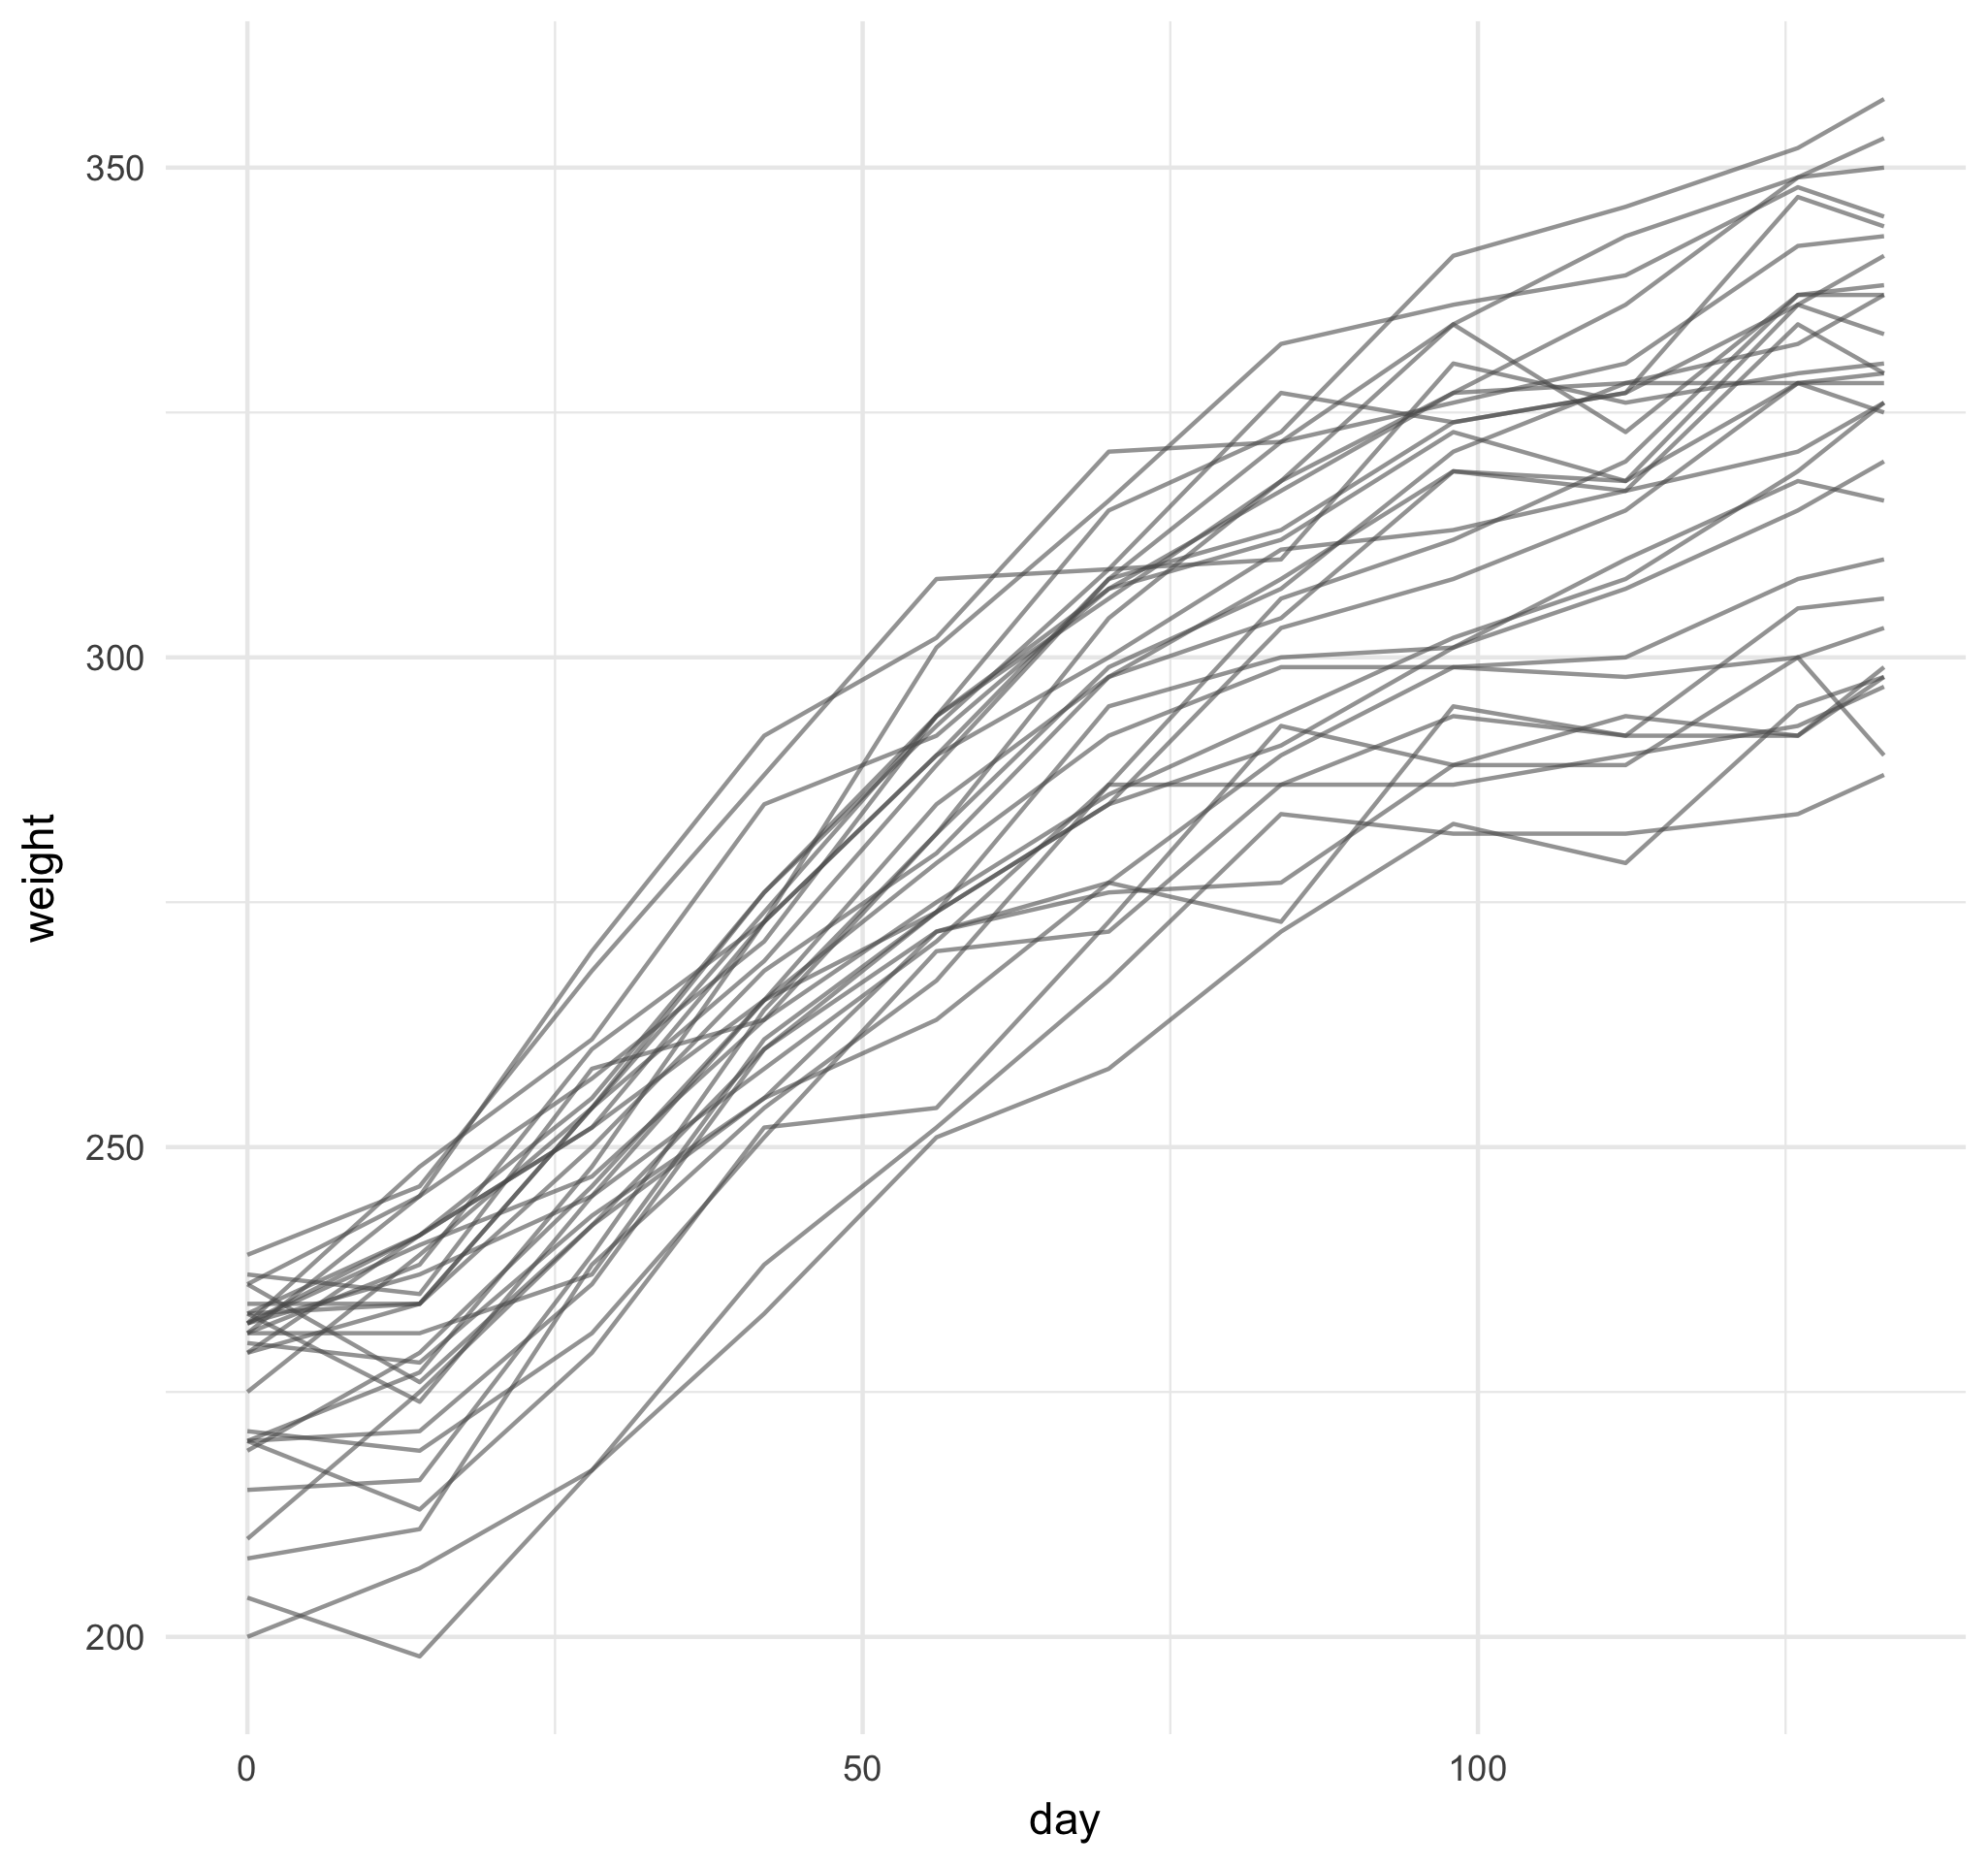
\includegraphics[width=.7\textwidth]{img/cattle/cattleA-weights-vs-time}
%\end{center}
% \caption{\textit{Weight trajectories over the observation period for experimental units in treatment group A.}}\label{fig:cattleA-weights-vs-time}
% \end{figure}

\begin{figure}[H] 
\begin{center}
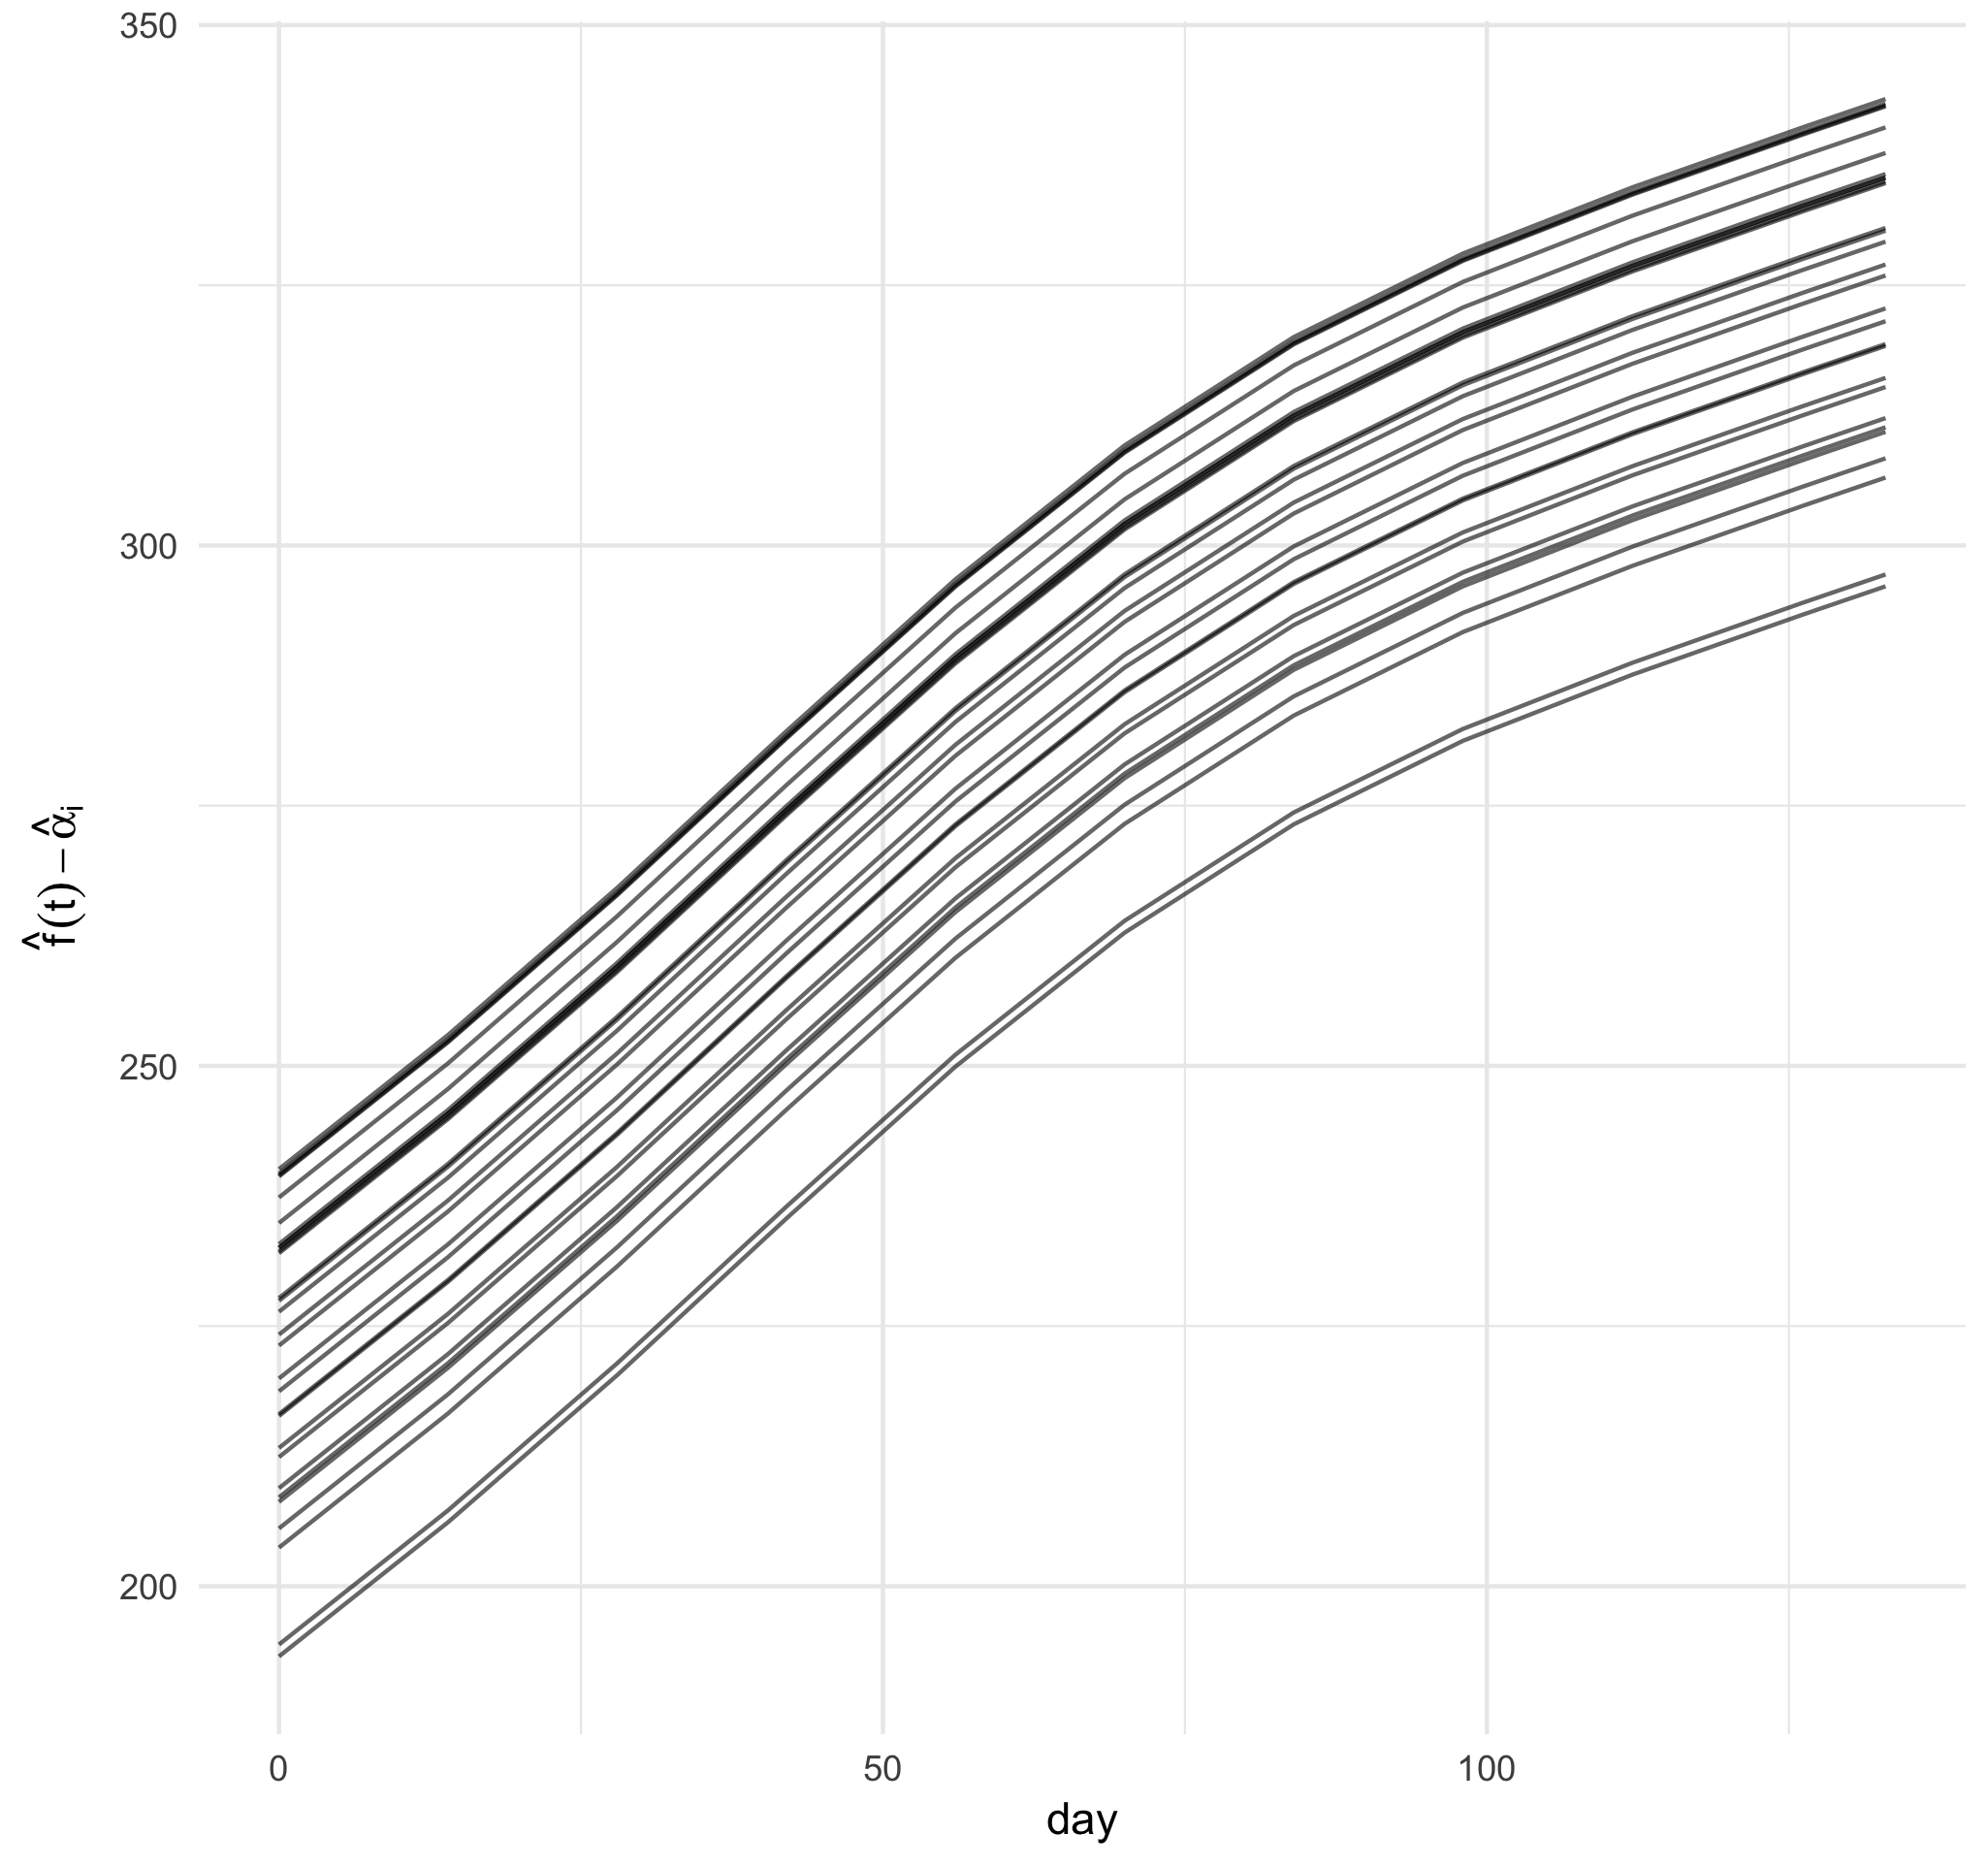
\includegraphics[width = .7\textwidth]{img/cattle/cattleA-weights-vs-time-mean-fit}
\caption{\textit{Subject-specific fitted weight trajectories for cattle in treatment group A. }}
\label{fig:cattleA-smoothed-weights-vs-time}
\end{center}
\end{figure} 
Centering the data using the fitted mean, the residuals 
\begin{equation} \label{eq:cattleA-dynamic-cond-mixed-model-2}
\epsilon^*\left(t_{ij}\right) = y\left(t_{ij}\right) - \left(f\left(t_{ij} \right) + \alpha_{i}\right)
\end{equation}
\noindent
serve as the data for estimating the functions defining the Cholesky factor and innovation variances. We model
\begin{equation} \label{eq:cattleA-dynamic-cond-mixed-model-1}
\epsilon^*\left(t_{ij}\right) = \sum_{k < j} \tilde{\phi}\left( t_{ij}, t_{ik} \right) \epsilon^*\left(t_{ik}\right) + \epsilon\left(t_{ij}\right)
\end{equation}
\noindent
where $\epsilon$ is a mean zero Gaussian process with variance $\sigma^2\left(t\right)$.

\bigskip

Choice of penalty is critical for convergence of the iterative estimation of $\tilde{\phi}$ and $\log\left(\sigma^2 \right)$. \cite{pan2017jmcm} concluded that the regressogram of empirical estimates of $\tilde{\phi}_{t,s}$ show consistent behaviour over $l = t - s$ for each value of $t$, indicating a lack of a strong functional component of $m$. This is consistent Pourahmadi's choice in the specification of model (\ref{eq:pourahmadi-cubic-model}) in terms of lag only. To balance the consideration of previous analyses with the interest of entirely data-driven model specification, we let $\phi \in \hilbert = \hilbert_{\left[l\right]} \otimes \hilbert_{\left[m\right]}$, where 
\begin{align*} 
\hilbert_{\left[l\right]} &= \bigg\{ \phi: \phi' = 0 \bigg\} \oplus \left\{\phi: \phi\left(0\right) = {\phi'}\left(0\right) = 0; \;\; \int {\phi}''\left(l\right)\;dl < \infty   \right\} \\
\hilbert_{\left[m\right]} &= \bigg\{ \phi: \phi \propto 1 \bigg\} \oplus \left\{ \phi: \int_0^1 \phi\left(m\right) \;dm = 0, \;\; \int {\phi}''\left(m\right)\;dm < \infty \right\} 
\end{align*} 
This decomposition leads to a null space comprised of functions of $l$ only, which is attractive because it coincides with the modeling assumptions made by \cite{pan2017jmcm}, \cite{huang2006covariance}, and \cite{wu2003nonparametric} for the same data set.  Figure~\ref{fig:fitted-cholesky-decomposition-cattle-date} shows the estimated Cholesky surface and innovation variance function evaluated at $t =  0,14, 28,\dots,112, 126,133$ and the corresponding pairs of observation times $\left(t,s\right)$, $0 \le s < t \le 133$. Figure~\ref{fig:cattle-fitted-cholesky-ssanova} shows $\hat{\phi}$ decomposed into the functional components of its ANOVA decomposition.


%\begin{figure}[H]
%\centering
%\subfloat[The sample regressogram for the cattle data from treatment group A, overlaid with a cubic polynomial smooth.]{
%  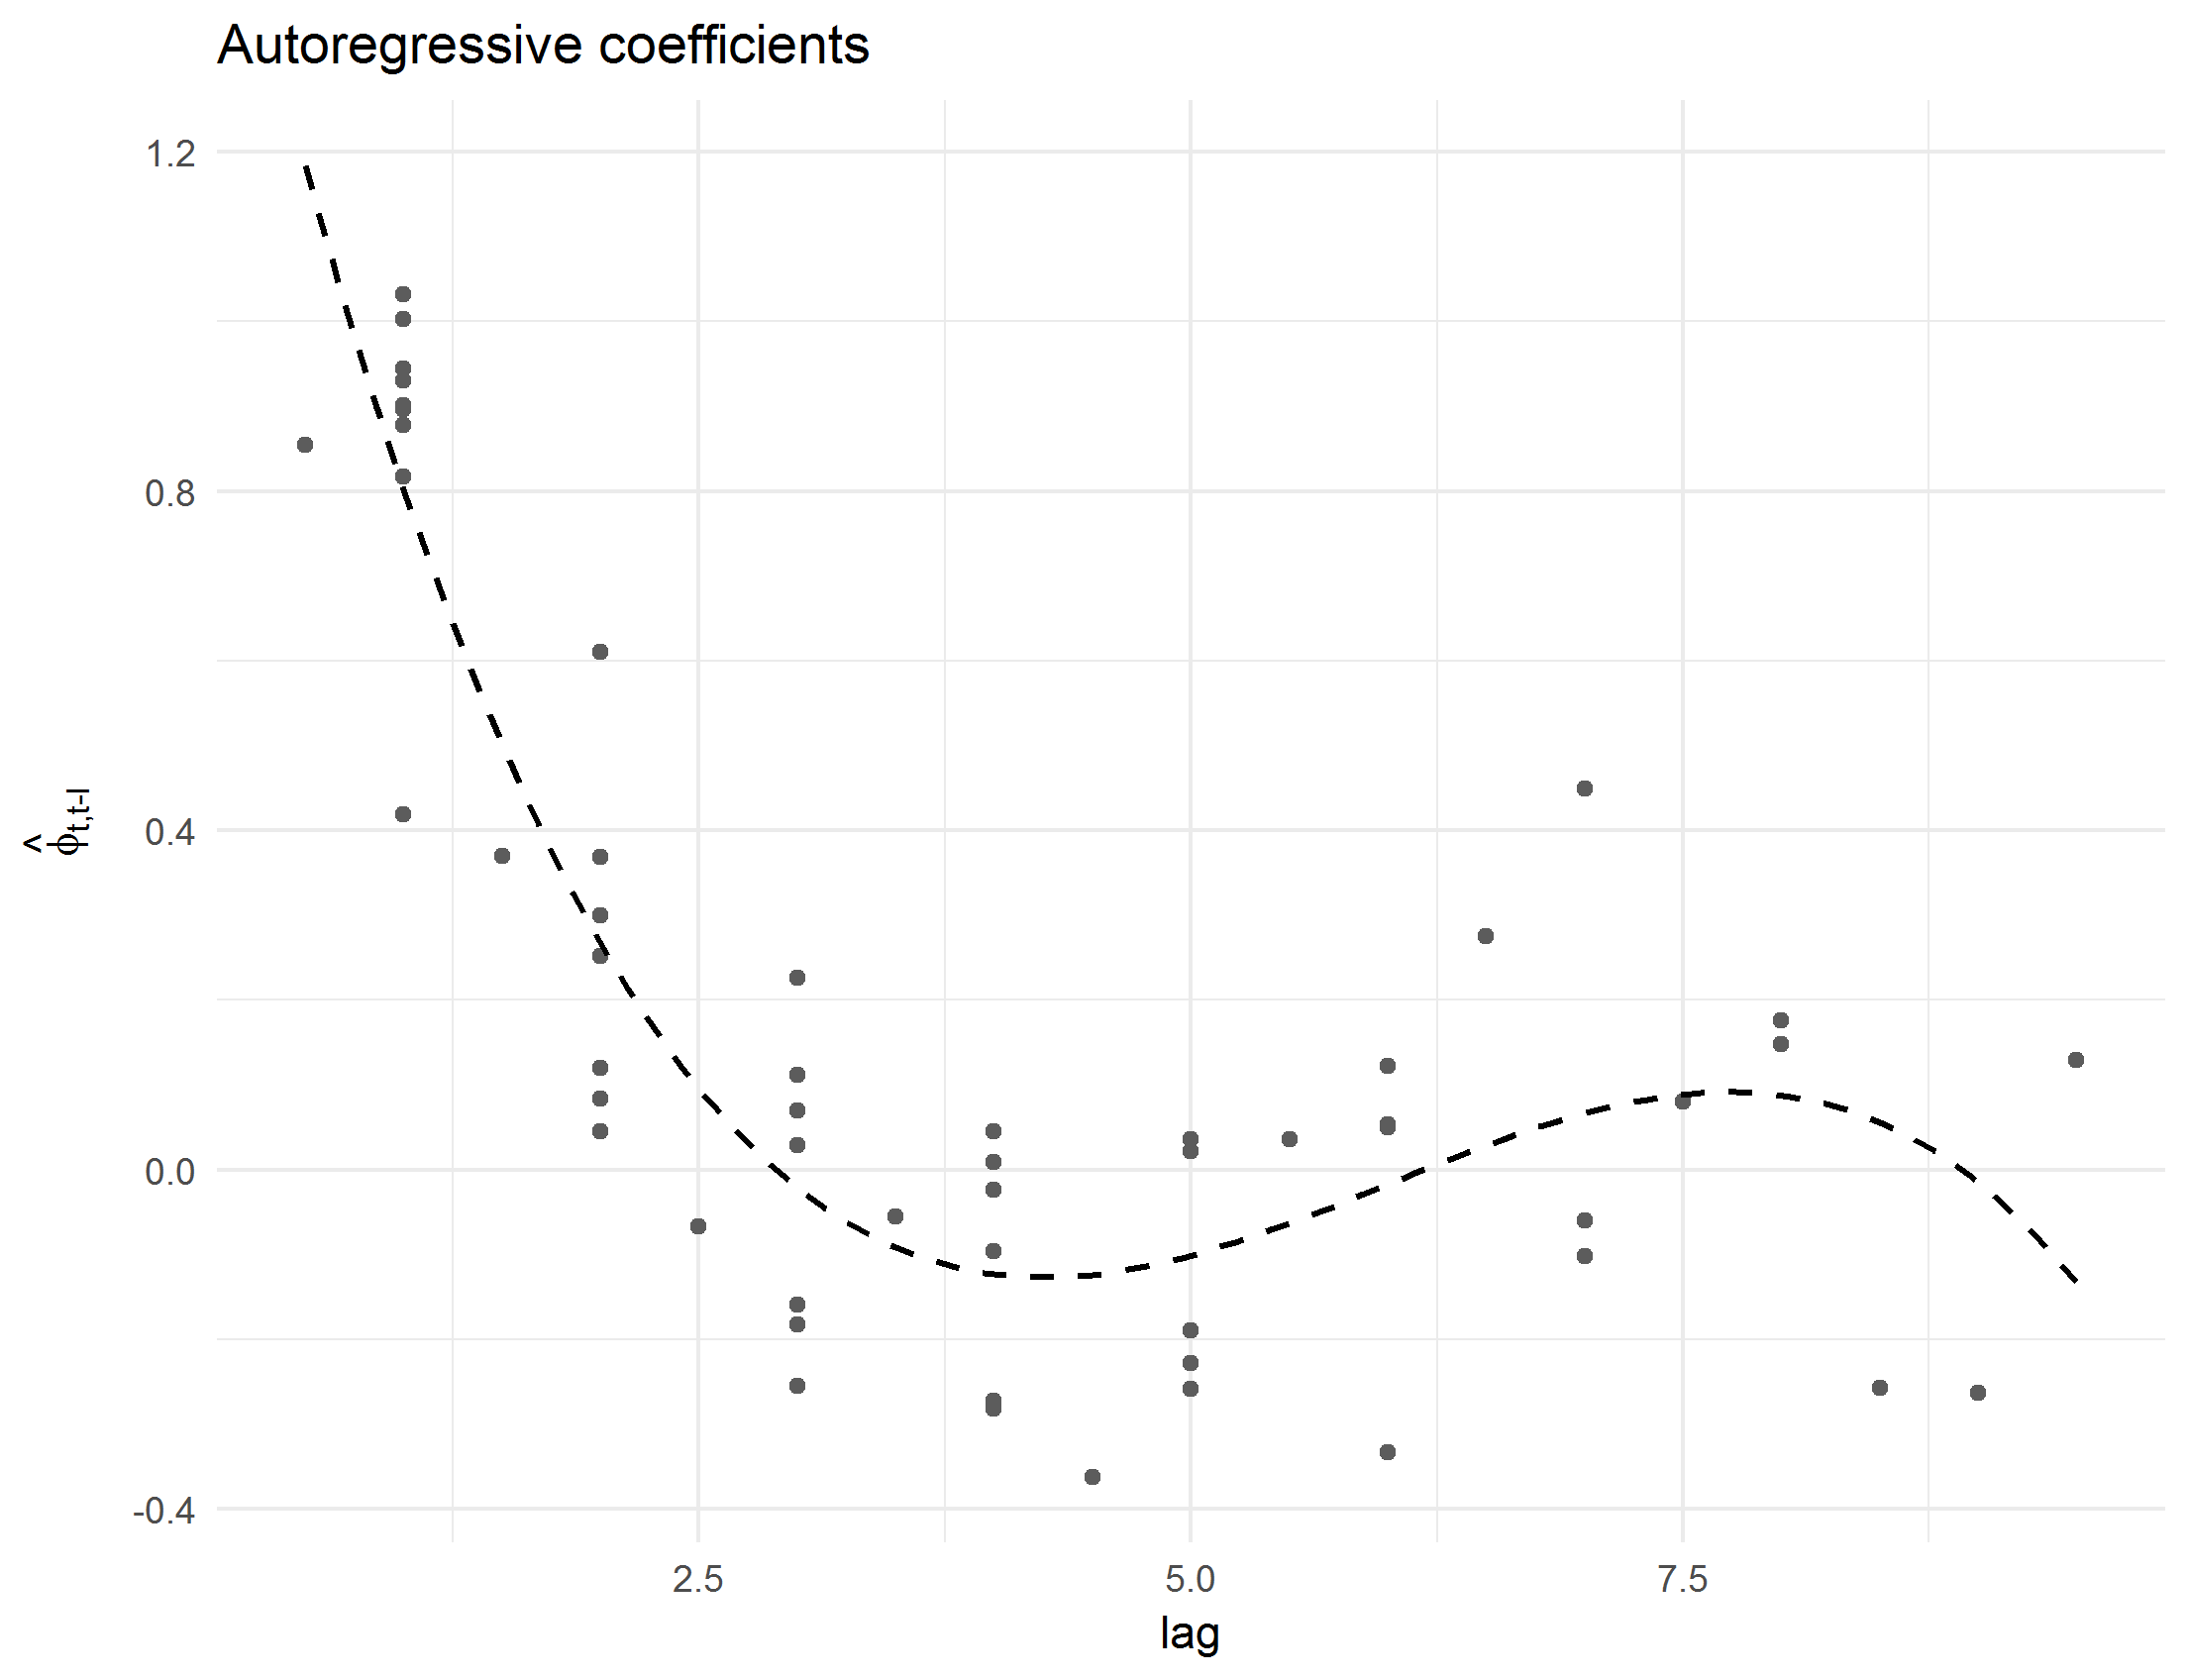
\includegraphics[width = .45\textwidth]{img/cattle/cattleA-regressogram-with-cubic-smooth}\label{fig:cattleA-regressogram-cubic-smooth}
%} 
%\hfill
%\subfloat[The sample variogram for the cattle data from treatment group A, overlaid with a cubic polynomial smooth.]{
%  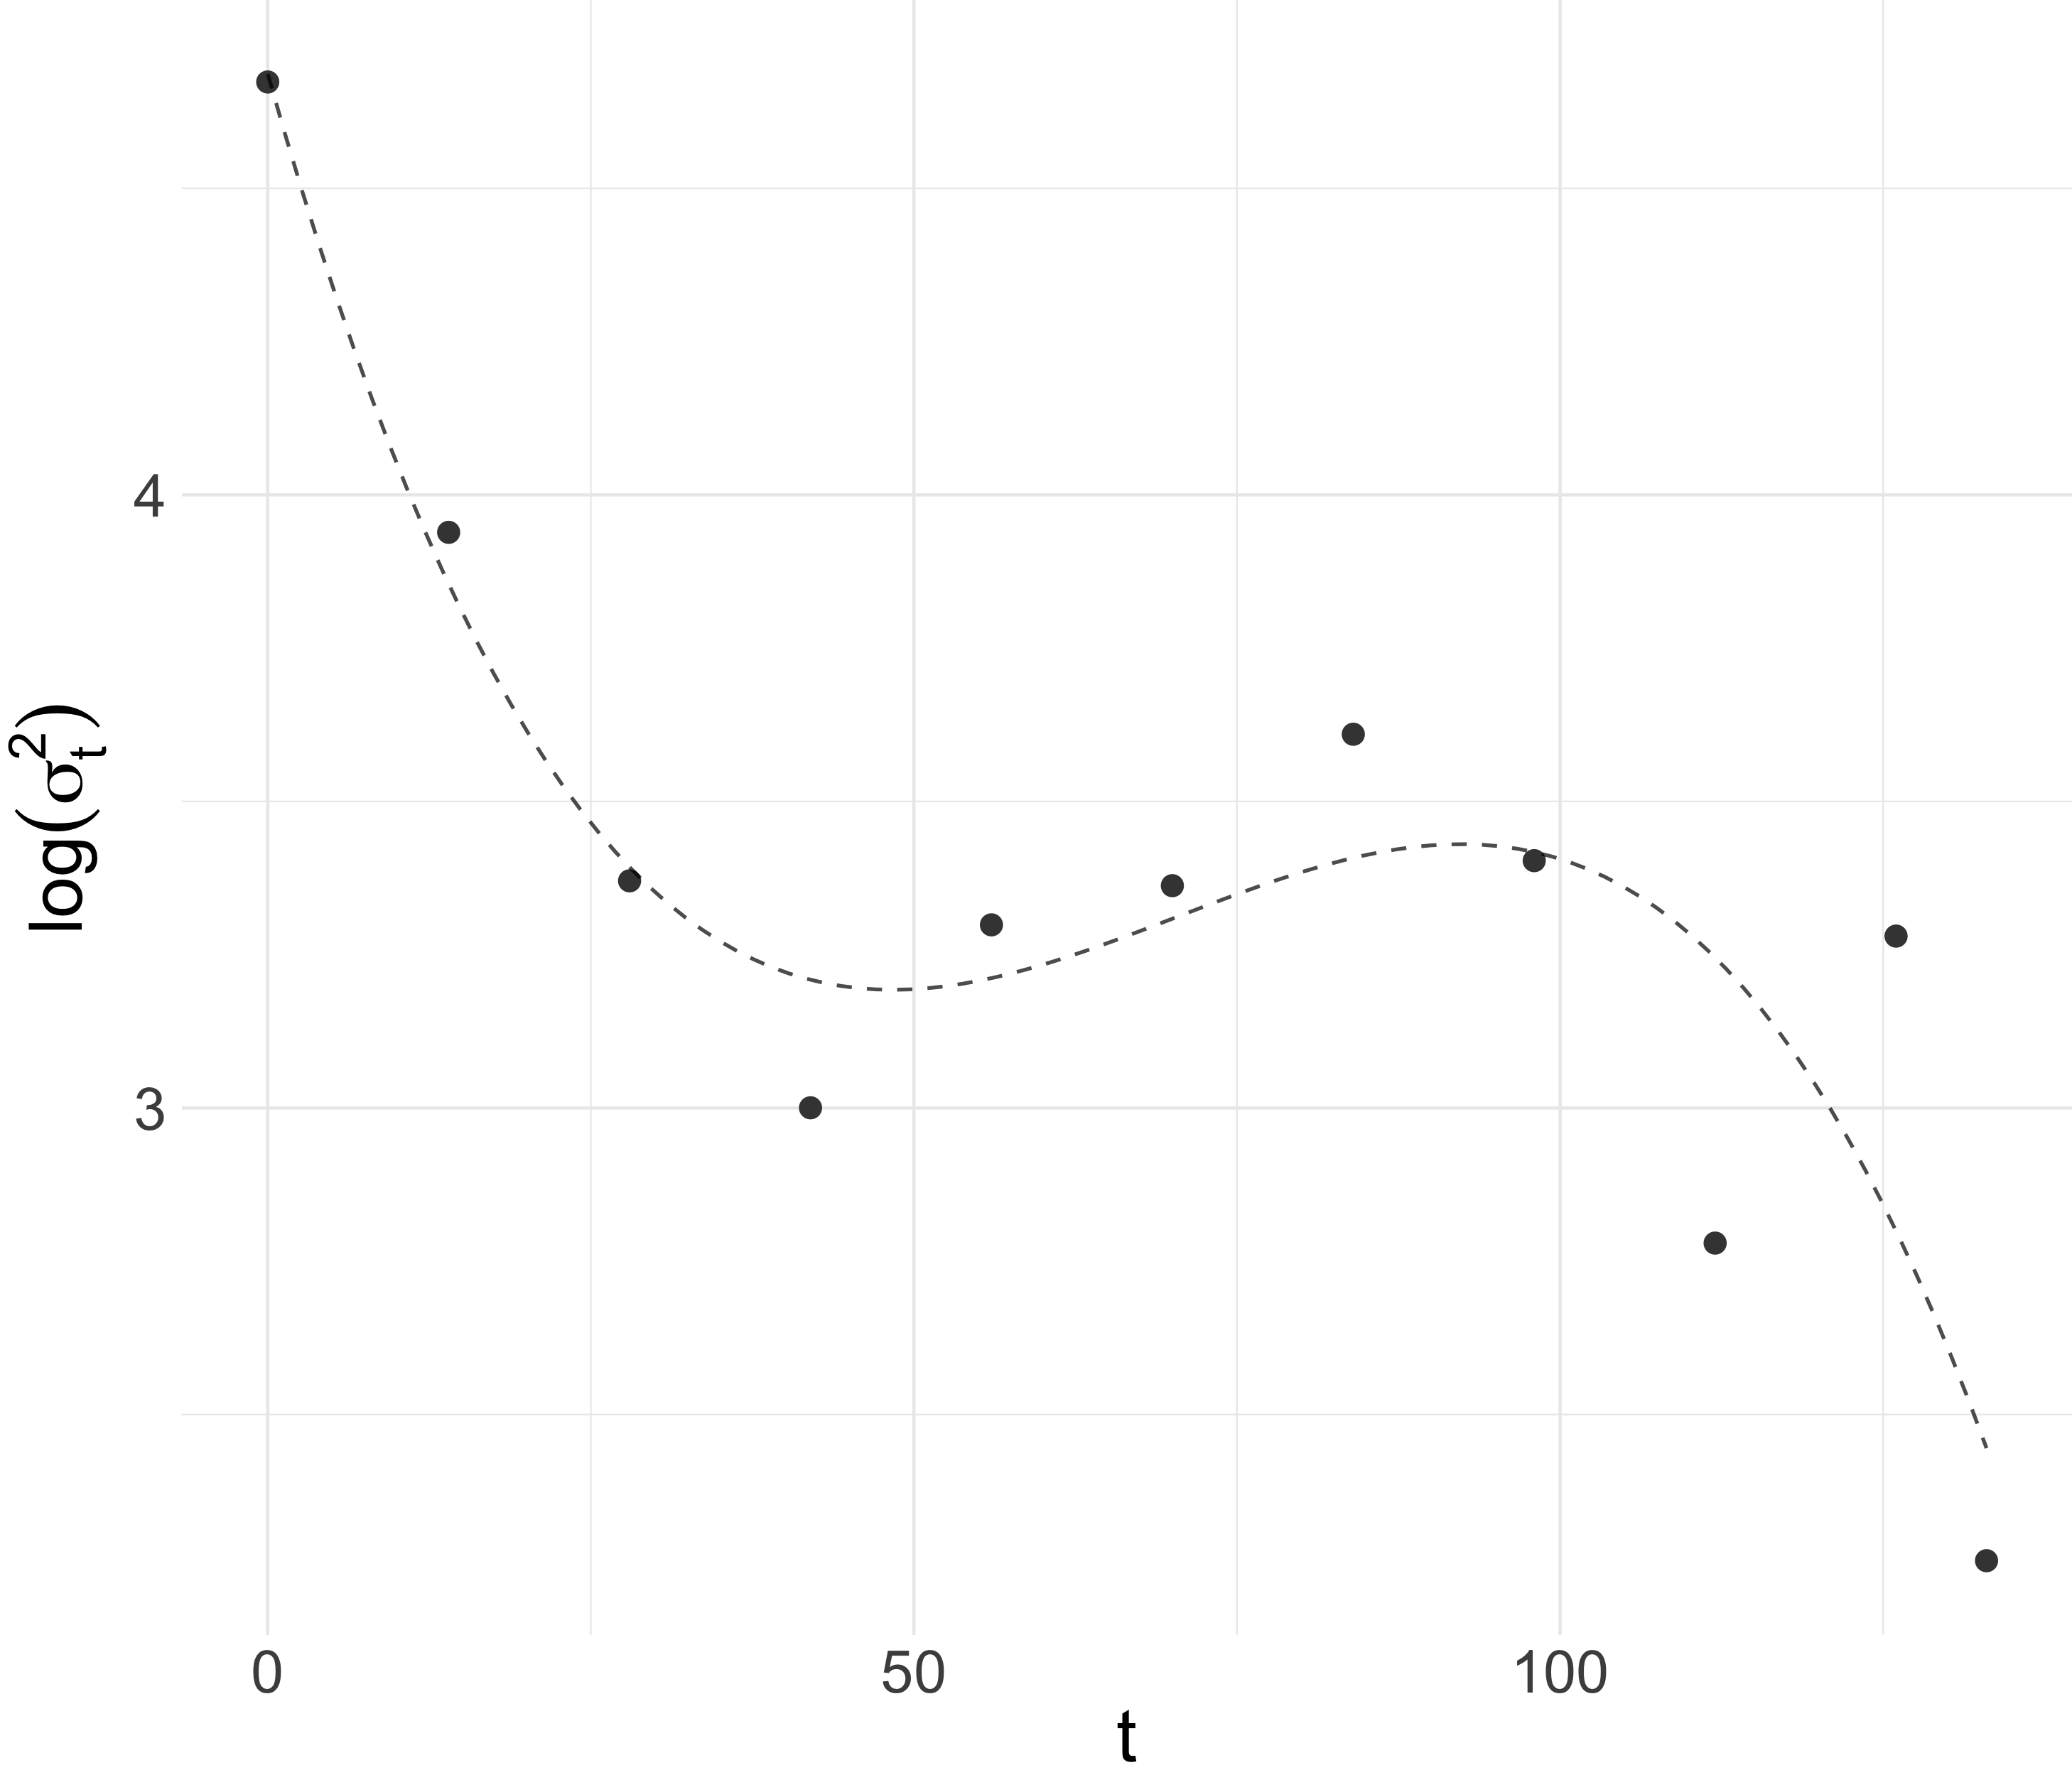
\includegraphics[width = .45\textwidth]{img/cattle/cattleA-innovariogram-with-cubic-smooth}\label{fig:cattleA-innovariogram-cubic-smooth}
%} 
%\end{figure}


%\begin{figure}[H]
% \begin{subfigure}{.33\textwidth}
%  \centering
%  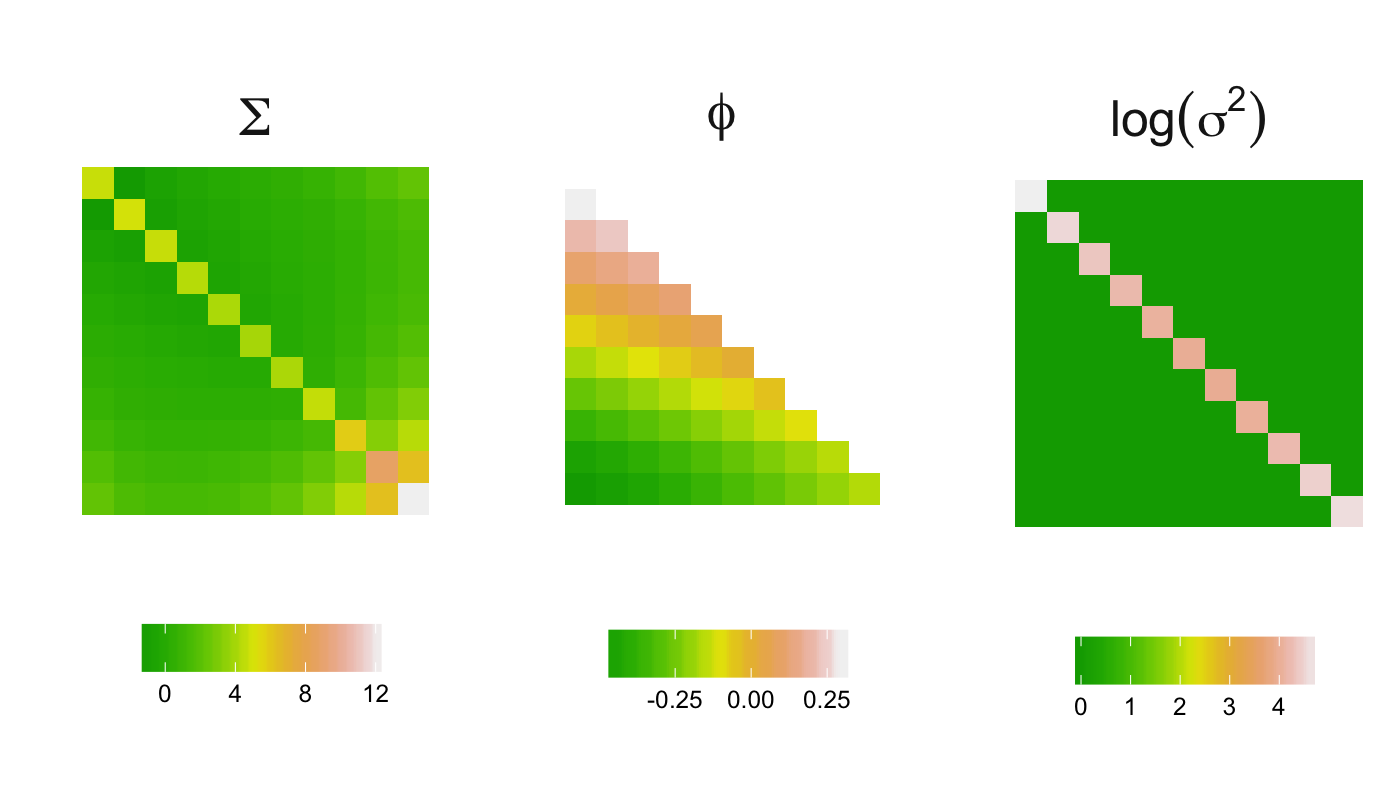
\includegraphics[width = \textwidth]{img/chapter-5/cattle-cholesky-estimate-ggplot}
% \caption{Estimated Cholesky factor $\hat{T}$}
% \end{subfigure}
% \begin{subfigure}{.33\textwidth}
%  \centering
%  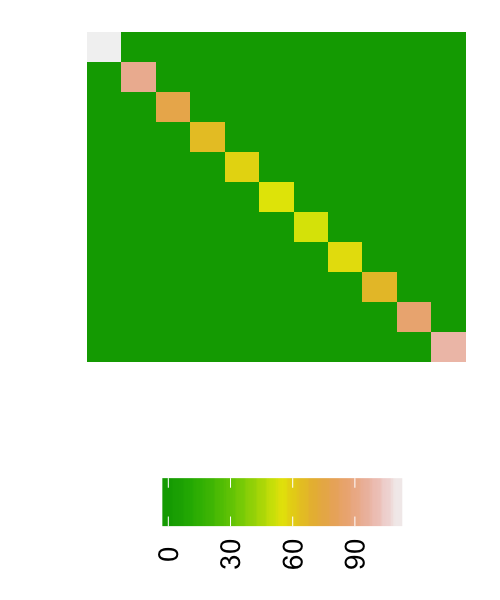
\includegraphics[width = \textwidth]{img/chapter-5/cattle-D-estimate-ggplot}
% \caption{Estimated innovation variances \newline $\hat{D} = diag\left( \sigma^2\left(t_1\right),\dots, \sigma^2\left(t_{11}\right) \right)$}
% \end{subfigure}
% \begin{subfigure}{.33\textwidth}
%  \centering
%  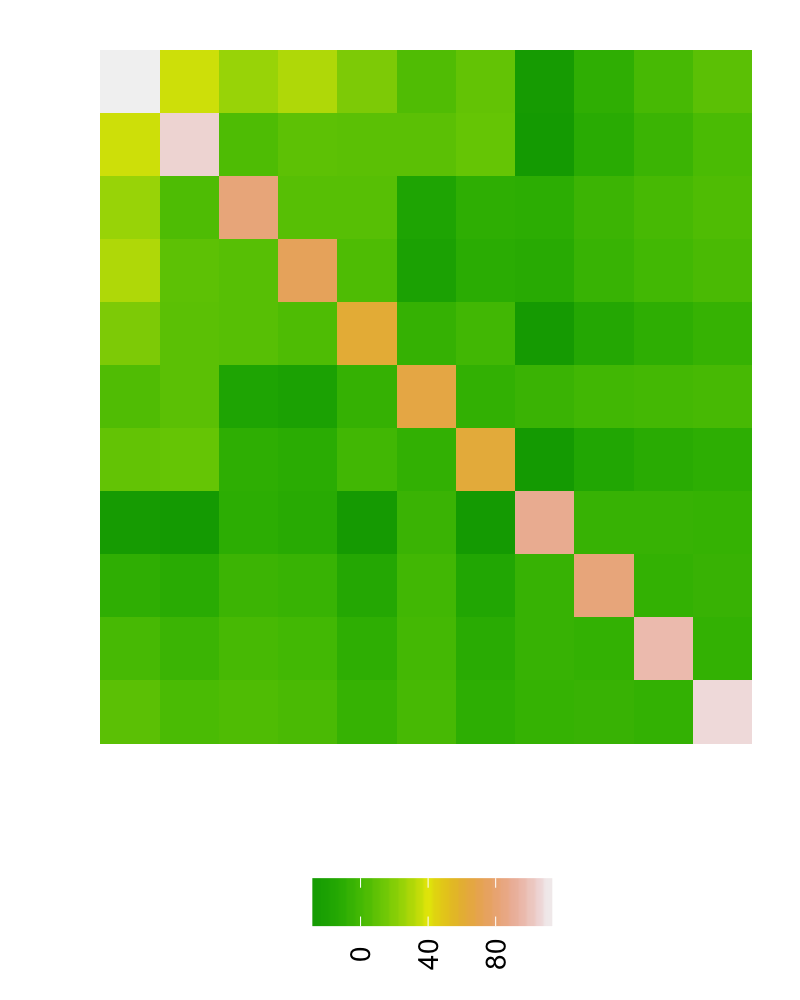
\includegraphics[width = \textwidth]{img/chapter-5/cattle-cov-estimate-ggplot}
% \caption{Estimated covariance matrix $\hat{\Sigma} = \hat{T}^{-1} \hat{D} {\hat{T}'}^{-1}$}
% \end{subfigure}
%\caption{Components of the fitted modified Cholesky decomposition for the cattle weight data.} \label{fig:fitted-cholesky-decomposition-cattle-date}
%\end{figure}
%
%
%\begin{figure}[H]
%  \centering
%  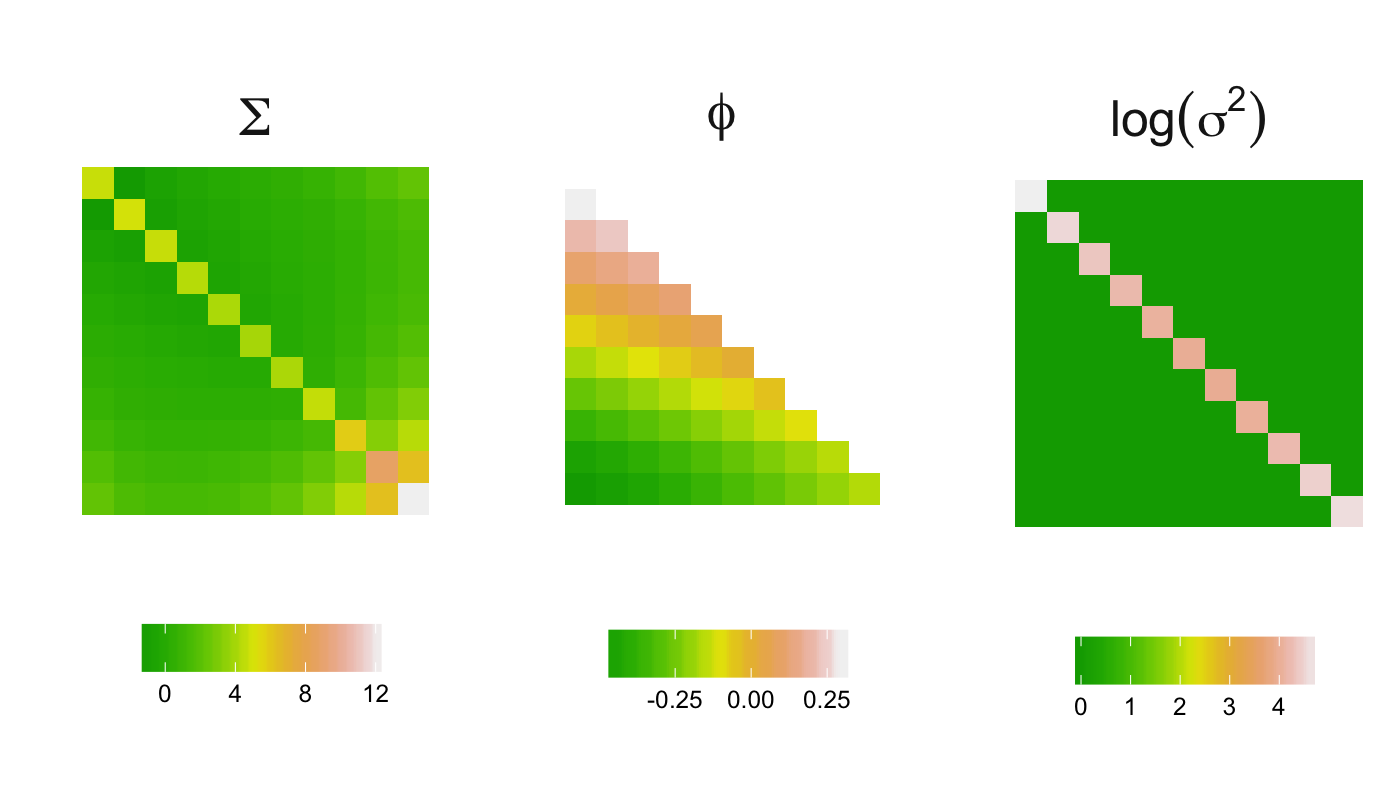
\includegraphics[width = \textwidth]{img/chapter-5/cattle-cholesky-estimate-ggplot}
%\caption{\textit{Components of the estimated covariance matrix for the cattle weight data from treatment group A: the sample covariance  }} \label{fig:fitted-cholesky-decomposition-cattle-date}
%\end{figure}

\begin{figure}[ht]
\centering
 \subfloat[\textit{$S$}]{\label{fig:fitted-cholesky-decomposition-cattle-date-S}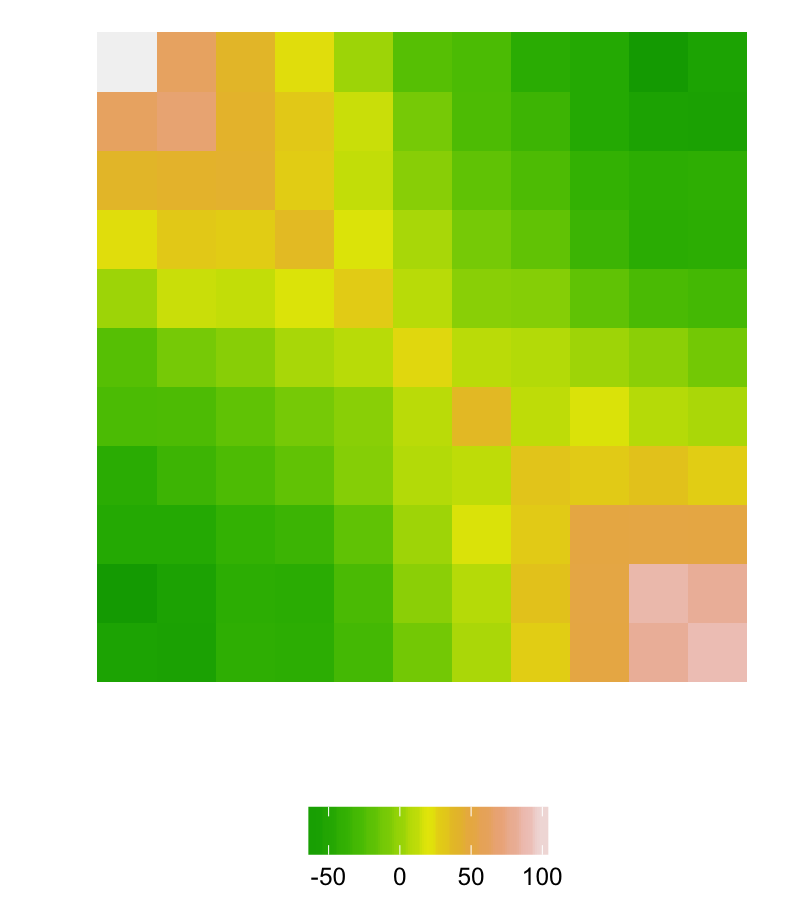
\includegraphics[width=0.35\textwidth]{img/chapter-5/cattle-cholesky-estimate-ggplot-S}}%\caption{\textit{$S$}}
    \subfloat[\textit{ $\hat{\Sigma} = \hat{T}^{-1} \hat{D} \hat{T}'^{-1} $}]{\label{fig:fitted-cholesky-decomposition-cattle-date-Sigma} 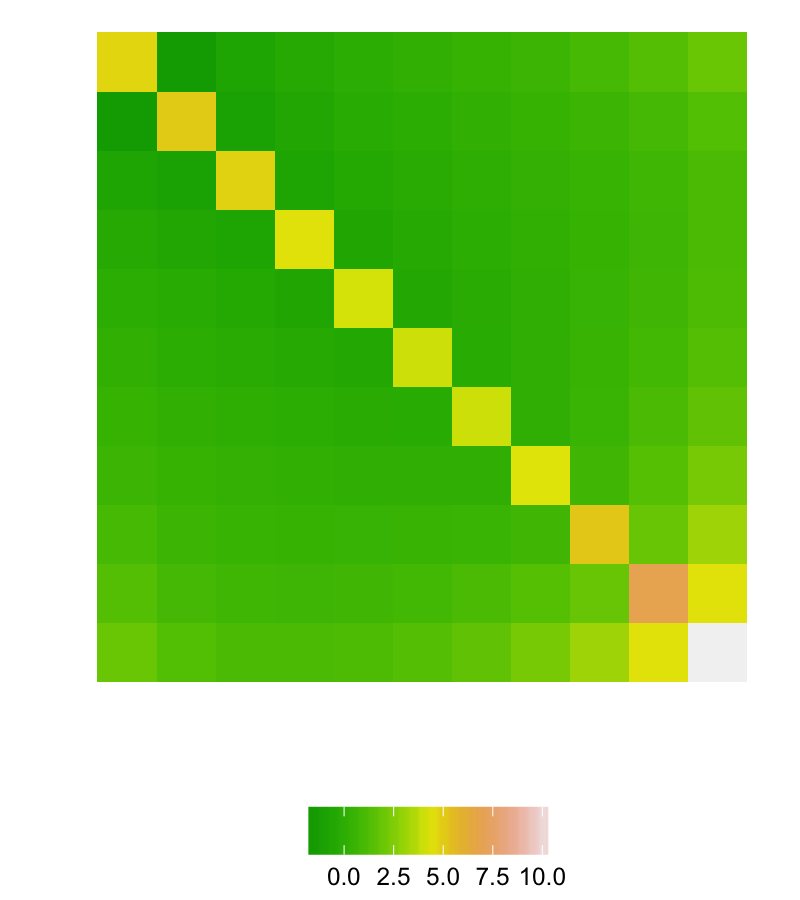
\includegraphics[width=0.35\textwidth]{img/chapter-5/cattle-cholesky-estimate-ggplot-Sigma}} \hfill
  \subfloat[\textit{$\hat{\phi}\left(t,s\right)$}]{\label{fig:fitted-cholesky-decomposition-cattle-date-phi} 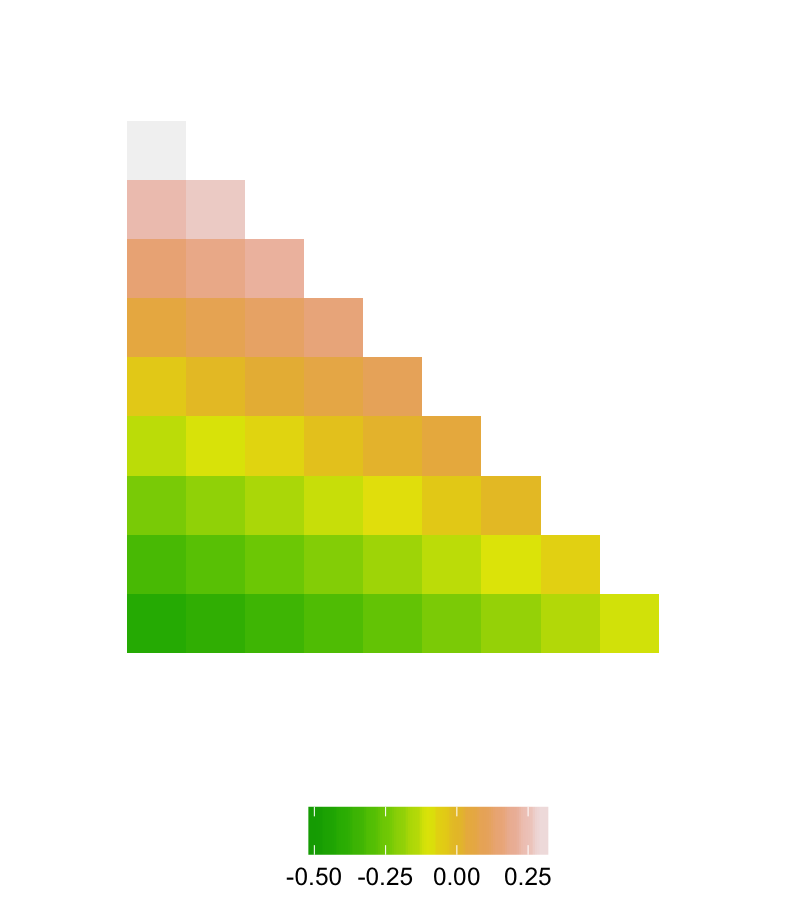
\includegraphics[width=0.35\textwidth]{img/chapter-5/cattle-cholesky-estimate-ggplot-phi}}%\label{fig:fitted-cholesky-decomposition-cattle-date-phi}
    \subfloat[\textit{$\log\hat{\sigma}^2\left(t\right)$}]{\label{fig:fitted-cholesky-decomposition-cattle-date-log-sigma2}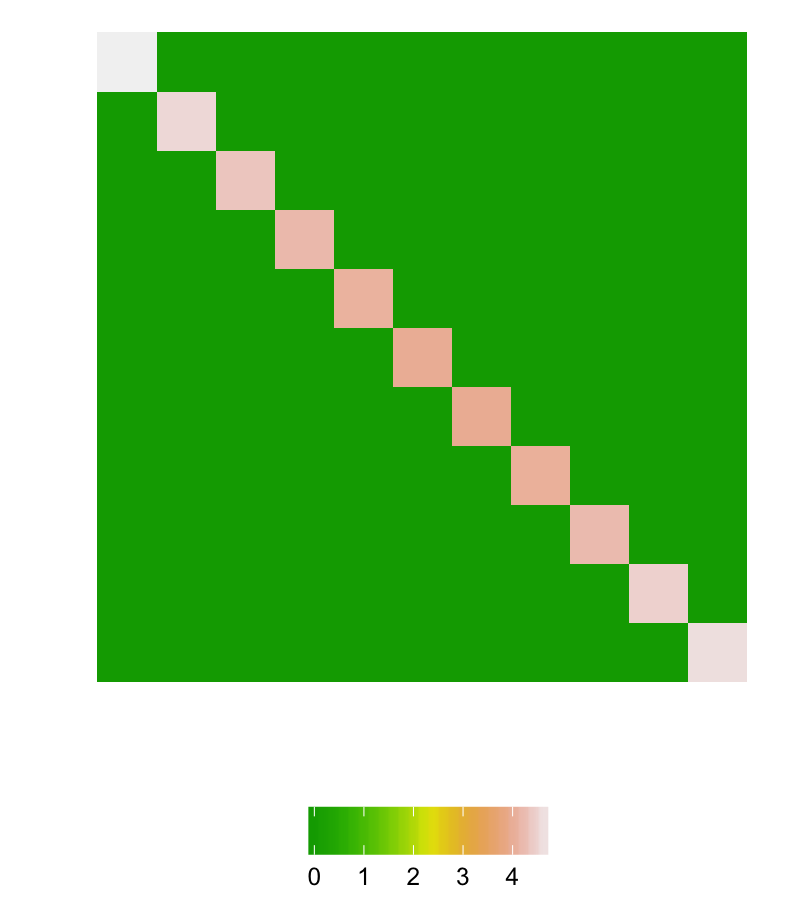
\includegraphics[width=0.35\textwidth]{img/chapter-5/cattle-cholesky-estimate-ggplot-log-sigma2} }
%  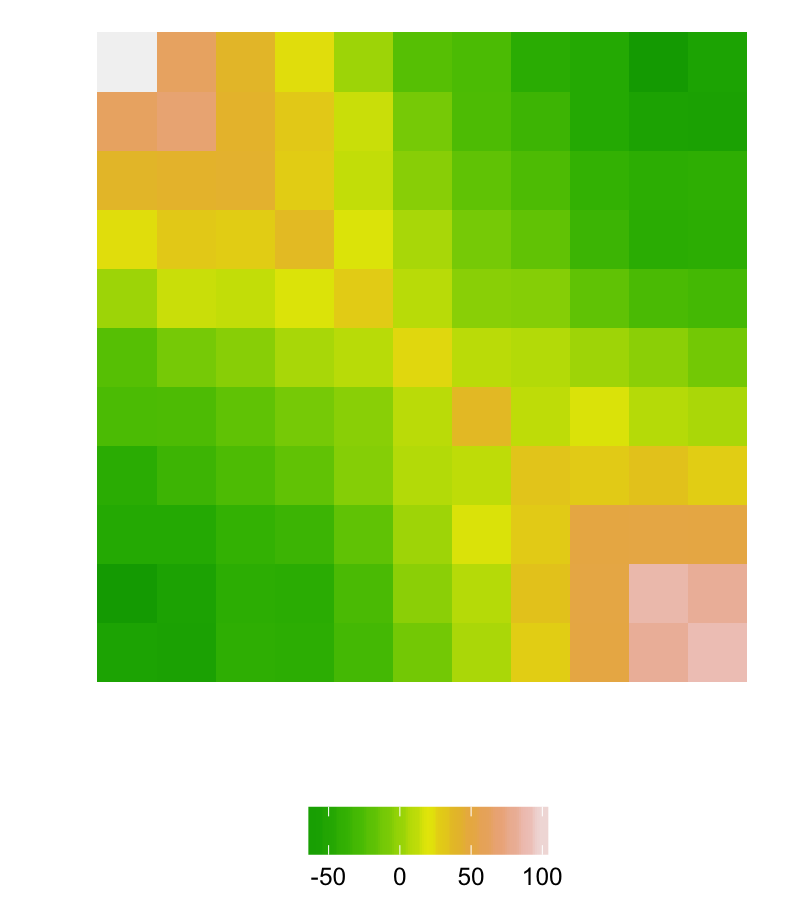
\includegraphics[width = \textwidth]{img/chapter-5/cattle-cholesky-estimate-ggplot-S}
% \caption{\textit{$S$}} \label{fig:fitted-cholesky-decomposition-cattle-data-S}
% \end{subfigure}
% \begin{subfigure}[t]{.35\textwidth}
%%  \centering
%  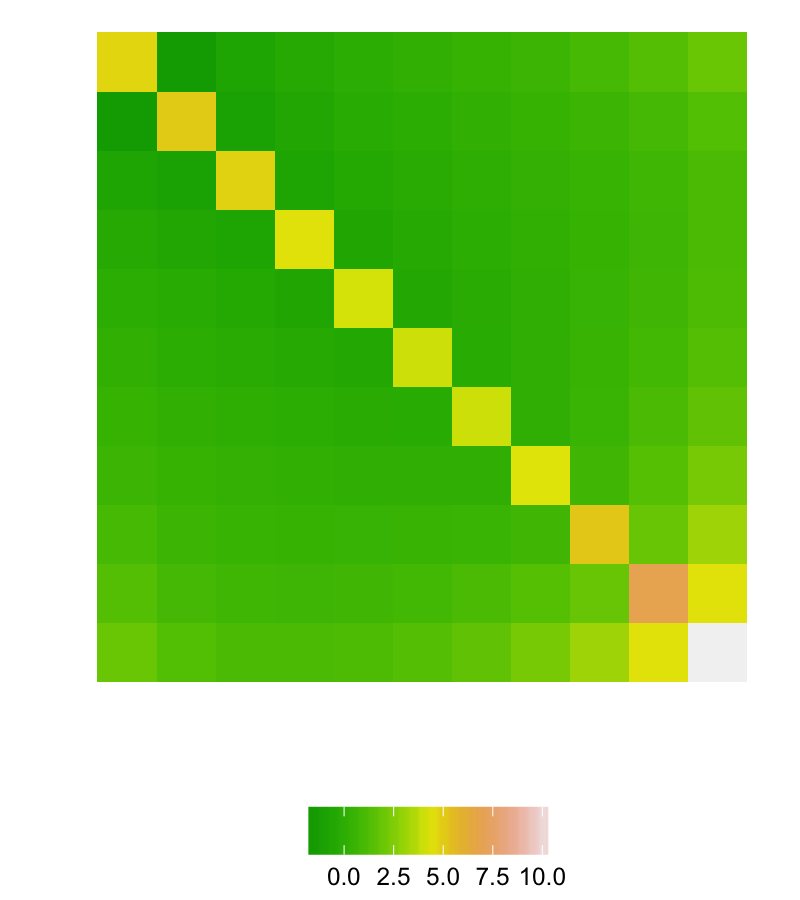
\includegraphics[width = \textwidth]{img/chapter-5/cattle-cholesky-estimate-ggplot-Sigma}
% \caption{\textit{ $\hat{\Sigma} = \hat{T}^{-1} \hat{D} \hat{T}'^{-1} $}}
%\label{fig:fitted-cholesky-decomposition-cattle-date-Sigma}
% \end{subfigure}
% \end{center}
% \hfill
% \begin{center}
%  \begin{subfigure}[t]{.35\textwidth}
%  \centering
%  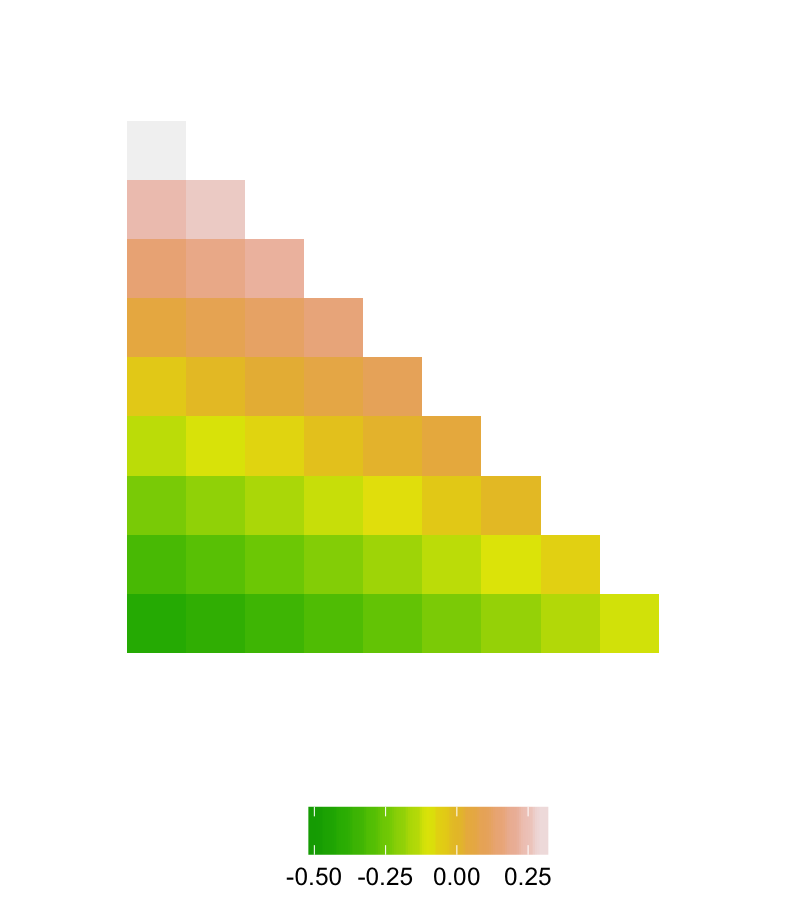
\includegraphics[width = \textwidth]{img/chapter-5/cattle-cholesky-estimate-ggplot-phi}
% \caption{\textit{$\hat{\phi}\left(t,s\right)$}} \label{fig:fitted-cholesky-decomposition-cattle-date-phi}
% \end{subfigure}
% \begin{subfigure}[t]{.35\textwidth}
% % \centering
%  \includegraphics[width = \textwidth]{img/chapter-5/cattle-cholesky-estimate-ggplot-log-sigma2}
% \caption{\textit{$\log\hat{\sigma}^2\left(t\right)$}}
%\label{fig:fitted-cholesky-decomposition-cattle-date-log-sigma2}
% \end{subfigure}
% \end{center}
 \caption{\textit{The sample covariance matrix $S$, the estimated covariance matrix for the cattle weight data from treatment group A and the estimated Cholesky decomposition of the covariance matrix. The generalized autoregressive coefficient function $\phi\left(t,s\right)$ and the log innovation variances $\log \sigma^2\left(t\right)$ were estimated using a tensor product cubic spline and cubic spline, respectively. The fitted functions define the components of the Cholesky factor $\hat{T}$ and diagonal matrix $\hat{D}$.}}  \label{fig:fitted-cholesky-decomposition-cattle-date}
\end{figure}


%\subfile{chapter-5-subfiles/cattle-cholesky-ssanova-ggplot}
\begin{figure}[H] 
\centering
  \includegraphics[width = 0.6\textwidth]{img/chapter-5/cattle-ssanova-estimate-lattice} 
  \caption{\textit{Components of the SSANOVA decomposition of the estimated generalized autoregressive coefficient function $\phi$ evaluated on the grid defined by the observed time points.}}\label{fig:cattle-fitted-cholesky-ssanova}
\end{figure}


Our sole focus on covariance estimation rather than the joint estimation of the mean and covariance makes apples-to-apples comparison with other analyses of the same dataset difficult. We constructed the mean estimate for the cattle in treatment group A shown in Figure~\ref{fig:cattleA-smoothed-weights-vs-time} entirely independently of the covariance estimate, which may be suboptimal compared to an iterative procedure that jointly estimates $f$, $b$, and $\Sigma$ as in \cite{pan2017jmcm} and \cite{pourahmadi1999joint}. Nevertheless, it is interesting to examine the differences between our estimates and cubic model fit shown in Figure~\ref{fig:cattleA-smoothed-regressogram-variogram}. Modeling $\phi$ as a polynomial in $l$ leaves any nonstationarity to be captured by the innovation variances. Of course, a model for the Cholesky factor having constant innovation variances and generalized autoregressive parameters which vary in $l$ only corresponds to a stationary process when certain conditions on the magnitude of the GARPs are satisfied \citep{klein1997statistical,madsen2007time}. Our estimated model instead captures the non-stationarity with both the log innovation variances as well as with $\phi_2$, the functional component corresponding to the main effect of $m$. The size of the functional components (in terms of the squared functional norm), however, does indicate a certain degree of concordance with the model proposed by \cite{pourahmadi1999joint}. The squared norm of the main effect of $l$ (1.914) is over twice that of the main effect of $m$ (0.790), and the squared norm of the interaction term, as clearly indicated by Figure~\ref{fig:cattle-fitted-cholesky-ssanova}, is negligible in comparison to the main effects.

%Evaluating the normal likelihood at the fitted model gives $\hat{\ell} = -818.5323$.


%\bibliography{../Master}
%
%\end{document}
 

\chapter{Concluding remarks and future work}\label{concluding-remarks-chapter}


%%%%%%%%%%%%%%%%%%%%%%%%%%%%%%%%%%%%%%%%%%%%%%%%%%%


Our formulation of covariance estimation supplies a flexible framework which free of the impediment presented by the positive definite constraint and a statistically intuitive interpretation of the elements of a covariance matrix. Modeling the Cholesky decomposition rather than the covariance matrix itself allows us to reframe covariance estimation as a regression problem.We estimate the parameters of the corresponding regression model using bivariate smoothing, and in doing so, we naturally accommodate irregularly-spaced longitudinal data of varying within-subject sample sizes by without the need for data imputation methods. An attractive quality of the general estimation framework is that it permits the flexibility of specifying any choice of basis, so as to agree with the underlying surface (curve) to be estimated. 

\bigskip
%%%%%%%%%%%%%%%%%%%%%%%%%%%%%%%%%%%%%%%%%%%%%%%%%%%
We demonstrate covariance estimation within this framework with two proposed representations of $\left(\phi, \log\sigma^2\right)$ the functional components of the Cholesky decomposition. We present a smoothing spline model for the generalized autoregressive varying coefficient and the innovation variance function and demonstrate how to specify penalties on the functional components of the functional ANOVA decompositions to enforce regularization of the fitted components to so that under heavy penalization, the fitted components correspond to commonly recruited structured covariance models. We demonstrate the fitting procedure using tensor product B-splines as an alternative basis expansion and impose regularization with discrete different penalties on the basis coefficients. The discrete penalties, which are constructed independently of the basis, offer flexibility over the smoothing spline penalties and require little computational complexity to implement. Simulation studies illustrate the relative performance of the estimators based on each basis compared to alternative estimators proposed in the longitudinal data literature. We apply our method to data generated from a longitudinal experiment examining the effectiveness of two treatments for intestinal parasites in cattle as measured by subject body weight over time. For a single treatment group, our nonparametric estimator echoes some of the modeling assumptions made to specify parametric models in previous analysis of the same data.

%%%%%%%%%%%%%%%%%%%%%%%%%%%%%%%%%%%%%%%%%%%%%%%%%%%
\bigskip 


The versatility of the framework surrounding the two detailed approaches for estimating the Cholesky decomposition of a covariance matrix leaves a number of open questions pertaining to its use. More recently, a problem receiving attention is that of estimating separate $p\times p$ covariance matrices $\Sigma_1,\dots, \Sigma_k$ for $k$ groups, having covariance where $k$ and $p$ are potentially large. Often, there is not enough data to estimate separate $\Sigma_i$ well for each group.For example, many tasks in financial management including portfolio selection and risk management can be reduced to the prediction of a sequence of large $p \times p$ covariance matrices \citep{tsay2005analysis}. Our procedure to covariance estimation encourages exploration of this problem; the regression model associated with the Cholesky decomposition \eqref{eq:mcd-ar-model} can incorporate additional group-specific covariates. 

\bigskip

The smoothing spline estimator circumvents the need for knot selection since it is constructed using a basis function for each of the unique within-subject pairs of measurement times. This is suitable when there is a fixed set of measurement times and unbalanced date arise due to missing observations. For the case that there is little overlap in measurement times across subjects so that these times are ``nearly'' unique for each subject, the size of the set $\vert V \vert $ can be so large that the dimension of the kernel matrix $Q$ as defined in (\ref{eq:penalized-likelihood-vectorized}) presents serious computational problems. An infinite dimensional Hilbert space is not necessarily required for representing the unknown function to be estimated, since the penalty effectively enforces a low dimensional model space. Efficient approximation can be carrying out by using a subset of the elements in $V$ to represent the unknown function; Algorithm~\ref{alg:SSANOVA-algorithm} can directly accommodate such a low dimensional representation. \cite{kim2004smoothing} provides detailed discussion of the efficient approximation of $\hilbert$.

\bigskip

The construction of the penalty for the P-spline estimator is convenient and easily appended to the log likelihood, so introducing both shrinkage and smoothing to covariance estimation is trivial (though selecting multiple smoothing parameter is perhaps not). Combining shrinkage and smoothing may produce better estimates than using shrinkage and smoothing alone, so further investigation is a worthwhile endeavor. 

\bigskip

The connection between nonparametric regression modes and mixed models has long been established \citep{green1987penalized}, but the area has gained more interest with more recent developments in software for fitting mixed models. Most of the early work was based on smoothing splines, \cite{eilers1999discussion} pointed how to
interpret P-splines as a mixed model, prompting a number of works investigating P-splines as mixed models. \cite{lee2011p} proposed the use of P-splines within a mixed modeling framework to estimate multidimensional functions as a decomposition into smooth main effects and interactions. The smoothing parameters are interpreted as variances of random effects, so model estimation and smoothing parameter selection can be performed simultaneously using the stable and efficient algorithms and software that are available for mixed models. Restricted maximum likelihood (REML) has proven to be very useful as a model selection tool, often producing smoother fits than generalized cross validation due to its better resistance to over-fitting \citep{wand2003semiparametric}. 

\bigskip

Application of the mixed model framework presented in \cite{lee2011p} to estimation of $\phi$ is attractive, because it not only provides an avenue for stable smoothing parameter selection, it permits the decomposition of the tensor product into functional components as in the SSANOVA model presented in Chapter~\ref{SSANOVA-chapter}. Direct application of this approach, however, is inaccessible due to the deconstruction of the marginal B-spline bases to adjust for the triangular domain of the autoregressive varying coefficient. Figure~\ref{fig:triangle-domain} illustrates how to ``trim'' the pairs of B-splines that don't overlap with the domain of $\phi$, which lies on the triangle $0 < s < t< 1$. Trimming the basis inhibits identifiability of functional components, though in the case that an additive model is appropriate, this trimming is unnecessary and REML may be employed for model estimation.

\bigskip

Alternatively, bivariate B-splines inherit several of the appealing properties of univariate B-splines and are applicable in various modeling problems, particularly for those involving non-rectangular domains. They have been used extensively in the field of graphics for the construction of smooth surfaces over irregular domains, but thus have far received little attention in the field of statistics. However, a recent paper by \cite{zhou2014principal} employs a mixed effects model for the functional principal components as bivariate splines on triangulations for data observed on an irregular grid. The application of their ideas to covariance estimation presents a promising approach to estimation of the Cholesky decomposition via bivariate smoothing.  


       


\appendix
\chapter{Chapter 2 Appendix} \label{chapter-2-appendix}

\section{Proof of Theorem~\ref{theorem:finite-dimensional-minimizer}}

\begin{proof}%[Proof of Theorem~\ref{theorem:finite-dimensional-minimizer}]
Some detailed discussion of the components of the minimizer $\phi_\lambda$ is useful for the proof. Letting $\hilbert = \hilbert_0 + \hilbert_J$ with $\hilbert_0 \perp \hilbert_J$, with reproducing kernel
\[
Q\left(\bfv, \bfv^*\right) = Q_0\left(\bfv, \bfv^*\right) + Q_J\left(\bfv, \bfv^*\right),
\]
\noindent
where $Q_0$ is the RK for $\hilbert_0$ and  $Q_J$ is the RK for $\hilbert_J$. Then 

\begin{align}
\xi_{i}\left(\bfv\right) &= \langle \xi_{i}, Q_\bfv \rangle_\hilbert \nonumber \\
&= \langle P_J \psi_{i},  Q_\bfv \rangle_\hilbert = \langle \psi_{i}, P_J {Q}_\bfv \rangle_\hilbert \nonumber   \\
&= \langle \psi_{i}, {Q_J}_\bfv \rangle_\hilbert \nonumber  \\
&= L_{i} {Q_J}_\bfv.\nonumber 
\end{align}
\noindent
where ${Q_J}_\bfv$ is the representer for the evaluation functional at $\bfv$ in $\hilbert_J$.  Since $\langle \psi_{i} - \xi_{i}, \xi_{j} \rangle = 0$,
\[
\langle \xi_{i}, \xi_{j} \rangle_\hilbert = \langle \psi_{i}, \xi_{j} \rangle_\hilbert.
\]
\noindent
Therefore, we have that 
\[
\langle \xi_{i}, \xi_{j} \rangle_\hilbert = L_{i}\xi_{j} = L_{i\left(\bfv \right)}L_{j\left(\bfv^* \right)} Q_J\left(\bfv,\bfv^*\right).
\]

Let the minimizer $\phi_\lambda$ be of the form

\begin{equation} \label{eq:form-of-the-minimizer-phi-plus-rho}
\phi_\lambda = \sum_{\nu = 1}^{d_0} d_\nu \eta_\nu + \sum_{\bfv_{i} \in V} c_i \xi_i + \rho,
\end{equation}
\noindent
where $\rho \in \hilbert_J$ is perpendicular to $\eta_1,\dots, \eta_{d_0}, \xi_{1}, \dots, \xi_{\vert V \vert}$.  The properties of reproducing kernel Hilbert spaces give us that any element in $\hilbert$ permits such a representation. Using that 

\begin{align*}
L_{ijk} \phi &= \langle \phi\left(\cdot\right), Q\left(\bfv_{ijk}, \cdot\right) \rangle_\hilbert \\
&=  \langle  \sum_{\nu = 1}^{d_0} d_\nu \eta_\nu\left(\cdot\right) + \sum_{\bfv_{i} \in V} c_i \xi_i + \rho\left(\cdot\right), Q\left(\bfv_{ijk}, \cdot\right) \rangle_\hilbert \\
&= \langle  \sum_{\nu = 1}^{d_0} d_\nu \eta_\nu\left(\cdot\right) + \sum_{\bfv_{i} \in V} c_i \xi_i + \rho\left(\cdot\right), Q_0\left(\bfv_{ijk}, \cdot\right) \rangle_\hilbert + \langle \sum_{\nu = 1}^{d_0} d_\nu \eta_\nu\left(\cdot\right) + \sum_{\bfv_{i} \in V} c_i \xi_i + \rho\left(\cdot\right), Q_1\left(\bfv_{ijk}, \cdot\right) \rangle_\hilbert \\
&=  \langle  \sum_{\nu = 1}^{d_0} d_\nu \eta_\nu\left(\cdot\right) ,  Q_0\left(\bfv_{ijk}, \cdot\right) \rangle_\hilbert +  \langle   \sum_{\bfv_{i} \in V} c_i \xi_i  ,  Q_0\left(\bfv_{ijk}, \cdot\right) \rangle_\hilbert + \langle \rho\left(\cdot\right), Q_0\left(\bfv_{ijk}, \cdot\right) \rangle_\hilbert \\ 
&\phantom{=} + \langle  \sum_{\nu = 1}^{d_0} d_\nu \eta_\nu\left(\cdot\right) ,  Q_1\left(\bfv_{ijk}, \cdot\right) \rangle_\hilbert +  \langle   \sum_{\bfv_{i} \in V} c_i \xi_i  ,  Q_1\left(\bfv_{ijk}, \cdot\right) \rangle_\hilbert + \langle \rho\left(\cdot\right), Q_1\left(\bfv_{ijk}, \cdot\right) \rangle_\hilbert, 
\end{align*}
\noindent
where $\langle \rho\left(\cdot\right), Q_0\left(\bfv_{ijk}, \cdot\right) \rangle_\hilbert = \langle \rho\left(\cdot\right), Q_1\left(\bfv_{ijk}, \cdot\right) \rangle_\hilbert = 0$. Thus, substituting \eqref{eq:form-of-the-minimizer-phi-plus-rho} for $\phi$ into \eqref{eq:phi-penalized-sums-of-squares}, the penalized sums of squares, becomes

\begin{equation*} 
\sum_{i=1}^N \sum_{j=2}^{m_i} \sigma^{-2}_{ij}\left( y_{ij} - \sum_{k<j}\left( L_{ijk}\phi\right) y_{ik}  \right)^2 + \lambda \left(\vert \vert \sum_{\bfv_i \in V} c_i \xi_i \vert \vert_\hilbert^2 + \vert \vert \rho \vert \vert_\hilbert^2\right),
\end{equation*} 
\noindent
which is obviously minimized when $\vert \vert \rho \vert \vert^2 = 0$.
 
\end{proof}
 
%%-----------------------------------------------------------------------------------------------------------------------------------------------------------------------------------------------------------------------------------
%%-----------------------------------------------------------------------------------------------------------------------------------------------------------------------------------------------------------------------------------
%%-----------------------------------------------------------------------------------------------------------------------------------------------------------------------------------------------------------------------------------
%%-----------------------------------------------------------------------------------------------------------------------------------------------------------------------------------------------------------------------------------
%%-----------------------------------------------------------------------------------------------------------------------------------------------------------------------------------------------------------------------------------
%%-----------------------------------------------------------------------------------------------------------------------------------------------------------------------------------------------------------------------------------
%%-----------------------------------------------------------------------------------------------------------------------------------------------------------------------------------------------------------------------------------
%%-----------------------------------------------------------------------------------------------------------------------------------------------------------------------------------------------------------------------------------
%%-----------------------------------------------------------------------------------------------------------------------------------------------------------------------------------------------------------------------------------
%%-----------------------------------------------------------------------------------------------------------------------------------------------------------------------------------------------------------------------------------
%%-----------------------------------------------------------------------------------------------------------------------------------------------------------------------------------------------------------------------------------
%%-----------------------------------------------------------------------------------------------------------------------------------------------------------------------------------------------------------------------------------

%
%\section{Chapter 4: Simulation studies}
%\subsection{Quadratic risk estimates for simulation study 1}
%%%-----------------------------------------------------------------------------------------------------------------------------------------------------------------------------------------------------------------------------------
%%%-----------------------------------------------------------------------------------------------------------------------------------------------------------------------------------------------------------------------------------
%%%-----------------------------------------------------------------------------------------------------------------------------------------------------------------------------------------------------------------------------------
%%%-----------------------------------------------------------------------------------------------------------------------------------------------------------------------------------------------------------------------------------
%%\subfile{chapter-4-subfiles/simulation-study-1-quad-table-model-1}
%\begin{table}[H]
%\centering
%\caption{Multivariate normal simulations for model I. Estimated quadratic risk is reported for our smoothing spline ANOVA estimator and P-spline estimator, the oracle estimator for each covariance structure, the parametric polynomial estimator of Pan and MacKenzie (2003), the sample covariance matrix, the tapered sample covariance matrix,
%                                    and the soft thresholding estimator.}
%\begin{tabular}{lrrrrrrrr}
%& $M$ &$\hat{\Sigma}_{SS}$& $\hat{\Sigma}_{PS}$ &$\hat{\Sigma}_{oracle}$& $\hat{\Sigma}_{poly}$ & $S$ &$S^\omega$& $S^\lambda$ \\ 
%  \hline
%  $N = 50$ & $10$ & 0.0015 & 0.0052 & 0.0267 & 0.0912 & 0.3901 & 0.3864 & 0.3874 \\ 
%   & $20$ & 0.0010 & 0.0043 & 0.0459 & 0.0757 & 0.8371 & 0.7710 & 0.7716 \\ 
%   & $30$ & 0.0026 & 0.0036 & 0.0386 & 0.1109 & 1.2857 & 1.1937 & 1.2074 \\ 
% $N = 100$ & 10 & 0.0005 & 0.0010 & 0.0209 & 0.0426 & 0.2116 & 0.1676 & 0.1720 \\ 
%    &   $20$ & 0.0003 & 0.0011 & 0.0212 & 0.0376 & 0.4255 & 0.3902 & 0.3970 \\ 
%    &   $30$ & 0.0002 & 0.0011 & 0.0276 & 0.0313 & 0.5984 & 0.5790 & 0.5842 \\ 
%   \hline
%\end{tabular} 
%\label{table:simulation-1-quad-loss-sigma-1}
%\end{table}
%%%-----------------------------------------------------------------------------------------------------------------------------------------------------------------------------------------------------------------------------------
%%%-----------------------------------------------------------------------------------------------------------------------------------------------------------------------------------------------------------------------------------
%%%-----------------------------------------------------------------------------------------------------------------------------------------------------------------------------------------------------------------------------------
%%%-----------------------------------------------------------------------------------------------------------------------------------------------------------------------------------------------------------------------------------
%% latex table generated in R 3.4.3 by xtable 1.8-2 package
%% Tue Mar  6 11:10:18 2018
%\begin{table}[H]
%\centering
%\caption{Multivariate normal simulation-estimated quadratic risk  for model II.} 
%\begin{tabular}{lrrrrrrrr}
%& $M$ &$\hat{\Sigma}_{SS}$& $\hat{\Sigma}_{PS}$ &$\hat{\Sigma}_{oracle}$& $\hat{\Sigma}_{poly}$ & $S$ &$S^\omega$& $S^\lambda$ \\ 
%  \hline
%$N = 50$ & $10$ & 0.0483 & 0.0623 & 0.0792 & 7.0137 & 0.6269 & 0.8108 & 0.5770 \\ 
%    & $20$ & 0.7972 & 1.2456 & 0.4317 & 852.2787 & 2.7659 & 30.8197 & 36.1492 \\ 
%     & $30$ & 6.7921 & 12.8700 & 7.2129 & 96997.8508 & 21.0228 & 365.0301 & 1804.9695 \\ 
%     $N = 100$ & $10$ & 0.0254 & 0.0525 & 0.0580 & 7.0482 & 0.2683 & 0.4351 & 0.2665 \\ 
%    & $20$ & 0.2877 & 0.8153 & 0.2625 & 861.3937 & 1.3347 & 5.5170 & 7.3283 \\ 
%     & $30$ & 2.7399 & 6.9793 & 3.6619 & 101509.5641 & 8.4769 & 66.9461 & 420.2973 \\ 
%   \hline
%\end{tabular}
%\label{table:simulation-1-quad-loss-sigma-2}
%\end{table}
% 
%%\subfile{chapter-4-subfiles/simulation-study-1-quad-table-model-2}
%%%-----------------------------------------------------------------------------------------------------------------------------------------------------------------------------------------------------------------------------------
%%%-----------------------------------------------------------------------------------------------------------------------------------------------------------------------------------------------------------------------------------
%%%-----------------------------------------------------------------------------------------------------------------------------------------------------------------------------------------------------------------------------------
%%%-----------------------------------------------------------------------------------------------------------------------------------------------------------------------------------------------------------------------------------
%%\subfile{chapter-4-subfiles/simulation-study-1-quad-table-model-3}
%\begin{table}[H]
%\centering
%\caption{Multivariate normal simulation-estimated quadratic risk  for model III.} 
%\begin{tabular}{lrrrrrrrr}
%  & $M$ &$\hat{\Sigma}_{SS}$& $\hat{\Sigma}_{PS}$ &$\hat{\Sigma}_{oracle}$& $\hat{\Sigma}_{poly}$ & $S$ &$S^\omega$& $S^\lambda$ \\ 
%  \hline
%$N = 50$ & $10$ & 0.0656 & 0.0665 & 0.0697 & 3.4849 & 0.4977 & 0.6678 & 0.5858 \\ 
%    &    $20$ & 1.0095 & 0.9146 & 0.4706 & 426.0848 & 2.0716 & 4.8213 & 8.4099 \\ 
%    &    $30$ & 10.8782 & 8.1124 & 5.3699 & 50613.5638 & 16.5536 & 779.2829 & 1181.3770 \\ 
%     $N = 100$ & 10 & 0.0486 & 0.0363 & 0.0328 & 3.5437 & 0.2437 & 0.2929 & 0.2791 \\ 
%     & $20$ & 0.6260 & 0.3783 & 0.1958 & 416.1285 & 1.0193 & 1.5353 & 5.1553 \\ 
%     & $30$ & 5.9367 & 3.4576 & 2.2121 & 50821.3671 & 7.9582 & 14.2394 & 253.4296 \\ 
%   \hline
%\end{tabular}
%\label{table:simulation-1-quad-loss-sigma-3}
%\end{table}
%%%-----------------------------------------------------------------------------------------------------------------------------------------------------------------------------------------------------------------------------------
%%%-----------------------------------------------------------------------------------------------------------------------------------------------------------------------------------------------------------------------------------
%%%-----------------------------------------------------------------------------------------------------------------------------------------------------------------------------------------------------------------------------------
%%%-----------------------------------------------------------------------------------------------------------------------------------------------------------------------------------------------------------------------------------
%%\subfile{chapter-4-subfiles/simulation-study-1-quad-table-model-4}
%
%\begin{table}[H]
%\centering
%\caption{Multivariate normal simulation-estimated quadratic risk  for model IV.} 
%\begin{tabular}{lrrrrrrrr}
%  & $M$ &$\hat{\Sigma}_{SS}$& $\hat{\Sigma}_{PS}$ &$\hat{\Sigma}_{oracle}$& $\hat{\Sigma}_{poly}$ & $S$ &$S^\omega$& $S^\lambda$ \\ 
%  \hline
%$N = 50$ & 10 & 0.0153 & 0.0196 & 0.0053 & 0.2575 & 0.4420 & 0.4628 & 0.4620 \\ 
%  & $20$ & 0.0450 & 0.0154 & 0.0073 & 0.4384 & 0.7951 & 0.9184 & 0.9177 \\ 
%  & $30$ & 0.0893 & 0.0189 & 0.0072 & 0.6539 & 1.3363 & 1.3014 & 1.3013 \\ 
% $N = 100$ & 10 & 0.0112 & 0.0186 & 0.0031 & 0.2098 & 0.2136 & 0.2299 & 0.2295 \\ 
%    &    $20$ & 0.0420 & 0.0143 & 0.0027 & 0.4877 & 0.4509 & 0.4311 & 0.4307 \\ 
%    &    $30$ & 0.0792 & 0.0181 & 0.0035 & 0.6616 & 0.6263 & 0.6598 & 0.6589 \\ 
%   \hline
%\end{tabular}
%\label{table:simulation-1-quad-loss-sigma-4}
%\end{table}
%%%-----------------------------------------------------------------------------------------------------------------------------------------------------------------------------------------------------------------------------------
%%%-----------------------------------------------------------------------------------------------------------------------------------------------------------------------------------------------------------------------------------
%%%-----------------------------------------------------------------------------------------------------------------------------------------------------------------------------------------------------------------------------------
%%%-----------------------------------------------------------------------------------------------------------------------------------------------------------------------------------------------------------------------------------
%
%\begin{table}[H]
%\centering
%\caption{Multivariate normal simulation-estimated quadratic risk  for model V.} 
%\begin{tabular}{lrrrrrrrr}
% $N$ & $M$ &$\hat{\Sigma}_{SS}$& $\hat{\Sigma}_{PS}$ &$\hat{\Sigma}_{oracle}$& $\hat{\Sigma}_{poly}$ & $S$ &$S^\omega$& $S^\lambda$ \\ 
%  \hline
%   $N = 50$ & 10 & 0.3659 & 0.2456 & 0.1610 & 1.3738 & 0.8484 & 1.6174 & 0.8963 \\ 
%     & $20$ & 1.0146 & 0.8206 & 0.5236 & 2.8419 & 1.7324 & 3.0233 & 1.6375 \\ 
%     & $30$ & 1.5352 & 1.1507 & 0.4632 & 4.1877 & 2.5484 & 5.1546 & 2.6727 \\ 
%    $N = 100$ & 10 & 0.3091 & 0.2678 & 0.0813 & 1.2439 & 0.4175 & 1.0431 & 0.4922 \\ 
%      & $20$ & 0.9734 & 0.4111 & 0.1522 & 2.7280 & 0.7896 & 2.1932 & 0.8461 \\ 
%     & $30$ & 1.6032 & 0.7701 & 0.3656 & 3.8905 & 1.2577 & 3.5722 & 1.3270 \\ 
%   \hline
%\end{tabular}
%\label{table:simulation-1-quad-loss-sigma-5}
%\end{table}
%%\subfile{chapter-4-subfiles/simulation-study-1-quad-table-model-5}
%% latex table generated in R 3.4.3 by xtable 1.8-2 package
%% Tue Mar  6 11:10:25 2018
%%%-----------------------------------------------------------------------------------------------------------------------------------------------------------------------------------------------------------------------------------
%%%-----------------------------------------------------------------------------------------------------------------------------------------------------------------------------------------------------------------------------------
%%%-----------------------------------------------------------------------------------------------------------------------------------------------------------------------------------------------------------------------------------
%%%-----------------------------------------------------------------------------------------------------------------------------------------------------------------------------------------------------------------------------------
%
%
%\subsection{Quadratic risk estimates for simulation study 2}
%%%-----------------------------------------------------------------------------------------------------------------------------------------------------------------------------------------------------------------------------------
%%%-----------------------------------------------------------------------------------------------------------------------------------------------------------------------------------------------------------------------------------
%%%-----------------------------------------------------------------------------------------------------------------------------------------------------------------------------------------------------------------------------------
%%%-----------------------------------------------------------------------------------------------------------------------------------------------------------------------------------------------------------------------------------
%\begin{table}[H]
%\centering
%\caption{Model 1: Quadratic risk estimates and corresponding standard errors 
%             for the MCD smoothing spline ANOVA estimator via 100 simulated multivariate
%             normal sample of size $N = 50$
%             when 5\%, 7\%, and 9\% of the data are missing. Risk is reported for the estimator constructed using
%             the unbiased risk estimate and leave-one-subject-out cross validation are used for smoothing parameter selection.} 
%\begin{tabular}{lrrlrl}
%   $M$ & \% missing & \multicolumn{2} {c} {$\Delta_1(\hat{\Sigma}^{U}_{SS})$} & \multicolumn{2} {c} {$\Delta_1(\hat{\Sigma}^{V^*}_{SS})$}\\ \hline
%10 & 0.00 & 0.0009265743 & (1e-040) & 0.0013929180 & (2e-040) \\ 
%   & 0.05 & 0.0017013396 & (3e-040) & 0.0011392156 & (2e-040) \\ 
%   & 0.07 & 0.0013180691 & (2e-040) & 0.0014179527 & (2e-040) \\ 
%   \hline
% & 0.09 & 0.0019051797 & (2e-040) & 0.0010759292 & (2e-040) \\ 
%  15 & 0.00 & 0.0014140333 & (2e-040) & 0.0015083986 & (2e-040) \\ 
%   & 0.05 & 0.0010297818 & (1e-040) & 0.0014716107 & (2e-040) \\ 
%   \hline
% & 0.07 & 0.0015350683 & (3e-040) & 0.0013068047 & (2e-040) \\ 
%   & 0.09 & 0.0018375709 & (3e-040) & 0.0012133312 & (2e-040) \\ 
%  20 & 0.00 & 0.0009757769 & (2e-040) & 0.0008901316 & (1e-040) \\ 
%   \hline
% & 0.05 & 0.0009224688 & (1e-040) & 0.0005839169 & (1e-040) \\ 
%   & 0.07 & 0.0007680194 & (1e-040) & 0.0006763406 & (1e-040) \\ 
%   & 0.09 & 0.0007406254 & (1e-040) & 0.0009270686 & (1e-040) \\ 
%  \end{tabular}\label{table:simulation-study-2-quad-risk-model-1}
%\end{table}
%%\subfile{chapter-4-subfiles/simulation-study-2-quad-risk-model-1}
%%%-----------------------------------------------------------------------------------------------------------------------------------------------------------------------------------------------------------------------------------
%%%-----------------------------------------------------------------------------------------------------------------------------------------------------------------------------------------------------------------------------------
%%%-----------------------------------------------------------------------------------------------------------------------------------------------------------------------------------------------------------------------------------
%%%-----------------------------------------------------------------------------------------------------------------------------------------------------------------------------------------------------------------------------------
%%%-----------------------------------------------------------------------------------------------------------------------------------------------------------------------------------------------------------------------------------
%%%-----------------------------------------------------------------------------------------------------------------------------------------------------------------------------------------------------------------------------------
%%%-----------------------------------------------------------------------------------------------------------------------------------------------------------------------------------------------------------------------------------
%%%-----------------------------------------------------------------------------------------------------------------------------------------------------------------------------------------------------------------------------------
%%\subfile{chapter-4-subfiles/simulation-study-2-quad-risk-model-2}
%\begin{table}[H]
%\centering
%\caption{Model 2: Quadratic risk estimates and corresponding standard errors.} 
%\begin{tabular}{lrrlrl}
%   $M$ & \% missing & \multicolumn{2} {c} {$\Delta_1(\hat{\Sigma}^{U}_{SS})$} & \multicolumn{2} {c} {$\Delta_1(\hat{\Sigma}^{V^*}_{SS})$}\\ \hline
%10 & 0.00 & 0.0667855 & (0.0051) & 0.0506111 & (0.0033) \\ 
%   & 0.05 & 0.0556528 & (0.0033) & 0.0606226 & (0.0040) \\ 
%   & 0.07 & 0.0559094 & (0.0034) & 0.0582334 & (0.0036) \\ 
%   \hline
% & 0.09 & 0.0567996 & (0.0037) & 0.0569597 & (0.0034) \\ 
%  15 & 0.00 & 0.1816735 & (0.0130) & 0.2353608 & (0.0188) \\ 
%   & 0.05 & 0.1842752 & (0.0119) & 0.2162470 & (0.0164) \\ 
%   \hline
% & 0.07 & 0.2225236 & (0.0162) & 0.2039186 & (0.0147) \\ 
%   & 0.09 & 0.2914073 & (0.0283) & 0.2239119 & (0.0149) \\ 
%  20 & 0.00 & 0.7825688 & (0.0560) & 0.6797717 & (0.0393) \\ 
%   \hline
% & 0.05 & 1.0196188 & (0.0949) & 0.9072404 & (0.0694) \\ 
%   & 0.07 & 0.7106319 & (0.0453) & 0.8460652 & (0.0643) \\ 
%   & 0.09 & 0.7537178 & (0.0580) & 0.8142586 & (0.0618) \\ 
%  \end{tabular}\label{table:simulation-study-2-quad-risk-model-2}
%\end{table}
%%%-----------------------------------------------------------------------------------------------------------------------------------------------------------------------------------------------------------------------------------
%%%-----------------------------------------------------------------------------------------------------------------------------------------------------------------------------------------------------------------------------------
%%%-----------------------------------------------------------------------------------------------------------------------------------------------------------------------------------------------------------------------------------
%%%-----------------------------------------------------------------------------------------------------------------------------------------------------------------------------------------------------------------------------------
%%%-----------------------------------------------------------------------------------------------------------------------------------------------------------------------------------------------------------------------------------
%%%-----------------------------------------------------------------------------------------------------------------------------------------------------------------------------------------------------------------------------------
%%%-----------------------------------------------------------------------------------------------------------------------------------------------------------------------------------------------------------------------------------
%%%-----------------------------------------------------------------------------------------------------------------------------------------------------------------------------------------------------------------------------------
%%\subfile{chapter-4-subfiles/simulation-study-2-quad-risk-model-3}
%\begin{table}[H]
%\centering
%\caption{Model 3: Quadratic risk estimates and corresponding standard errors.} 
%\begin{tabular}{lrrlrl}
%   $M$ & \% missing & \multicolumn{2} {c} {$\Delta_1(\hat{\Sigma}^{U}_{SS})$} & \multicolumn{2} {c} {$\Delta_1(\hat{\Sigma}^{V^*}_{SS})$}\\ \hline
%10 & 0.00 & 0.0219924 & (0.0021) & 0.0474410 & (0.0059) \\ 
%   & 0.05 & 0.0413327 & (0.0043) & 0.0390815 & (0.0045) \\ 
%   & 0.07 & 0.0404115 & (0.0044) & 0.0333281 & (0.0034) \\ 
%   \hline
% & 0.09 & 0.0332642 & (0.0036) & 0.0285832 & (0.0029) \\ 
%  15 & 0.00 & 0.1493227 & (0.0192) & 0.1897041 & (0.0240) \\ 
%   & 0.05 & 0.1327721 & (0.0209) & 0.1893346 & (0.0233) \\ 
%   \hline
% & 0.07 & 0.1939995 & (0.0304) & 0.1499919 & (0.0201) \\ 
%   & 0.09 & 0.1614249 & (0.0218) & 0.1244167 & (0.0158) \\ 
%  20 & 0.00 & 0.4121676 & (0.0503) & 0.3912354 & (0.0507) \\ 
%   \hline
% & 0.05 & 0.5088004 & (0.0731) & 0.4557829 & (0.0573) \\ 
%   & 0.07 & 0.4321571 & (0.0619) & 0.3652646 & (0.0415) \\ 
%   & 0.09 & 0.3996033 & (0.0477) & 0.3571157 & (0.0569) \\ 
%  \end{tabular}\label{table:simulation-study-2-quad-risk-model-3}
%\end{table}
%%%-----------------------------------------------------------------------------------------------------------------------------------------------------------------------------------------------------------------------------------
%%%-----------------------------------------------------------------------------------------------------------------------------------------------------------------------------------------------------------------------------------
%%%-----------------------------------------------------------------------------------------------------------------------------------------------------------------------------------------------------------------------------------
%%%-----------------------------------------------------------------------------------------------------------------------------------------------------------------------------------------------------------------------------------
%
%%%-----------------------------------------------------------------------------------------------------------------------------------------------------------------------------------------------------------------------------------
%%%-----------------------------------------------------------------------------------------------------------------------------------------------------------------------------------------------------------------------------------
%%%-----------------------------------------------------------------------------------------------------------------------------------------------------------------------------------------------------------------------------------
%%%-----------------------------------------------------------------------------------------------------------------------------------------------------------------------------------------------------------------------------------
%%\subfile{chapter-4-subfiles/simulation-study-2-quad-risk-model-4}
%\begin{table}[H]
%\centering
%\caption{Model 4: Quadratic risk estimates and corresponding standard errors.} 
%\begin{tabular}{lrrlrl}
%   $M$ & \% missing & \multicolumn{2} {c} {$\Delta_1(\hat{\Sigma}^{U}_{SS})$} & \multicolumn{2} {c} {$\Delta_1(\hat{\Sigma}^{V^*}_{SS})$}\\ \hline
%10 & 0.00 & 0.01413389 & (6e-040) & 0.01423523 & (5e-040) \\ 
%   & 0.05 & 0.01474523 & (7e-040) & 0.01340456 & (5e-040) \\ 
%   & 0.07 & 0.01410561 & (7e-040) & 0.01320081 & (6e-040) \\ 
%   \hline
% & 0.09 & 0.01415638 & (5e-040) & 0.01265559 & (4e-040) \\ 
%  15 & 0.00 & 0.03044151 & (0.0012) & 0.02958915 & (0.0010) \\ 
%   & 0.05 & 0.02932117 & (0.0010) & 0.02854528 & (8e-040) \\ 
%   \hline
% & 0.07 & 0.02950376 & (0.0010) & 0.02879928 & (7e-040) \\ 
%   & 0.09 & 0.02820952 & (9e-040) & 0.03032463 & (0.0010) \\ 
%  20 & 0.00 & 0.04691149 & (0.0012) & 0.04356297 & (4e-040) \\ 
%   \hline
% & 0.05 & 0.04540770 & (8e-040) & 0.04662982 & (9e-040) \\ 
%   & 0.07 & 0.04637991 & (0.0011) & 0.04443208 & (6e-040) \\ 
%   & 0.09 & 0.04474288 & (8e-040) & 0.04526569 & (6e-040) \\ 
%  \end{tabular}\label{table:simulation-study-2-quad-risk-model-4}
%\end{table}
%%%-----------------------------------------------------------------------------------------------------------------------------------------------------------------------------------------------------------------------------------
%%%-----------------------------------------------------------------------------------------------------------------------------------------------------------------------------------------------------------------------------------
%%%-----------------------------------------------------------------------------------------------------------------------------------------------------------------------------------------------------------------------------------
%%%-----------------------------------------------------------------------------------------------------------------------------------------------------------------------------------------------------------------------------------
%
%%%-----------------------------------------------------------------------------------------------------------------------------------------------------------------------------------------------------------------------------------
%%%-----------------------------------------------------------------------------------------------------------------------------------------------------------------------------------------------------------------------------------
%%%-----------------------------------------------------------------------------------------------------------------------------------------------------------------------------------------------------------------------------------
%%%-----------------------------------------------------------------------------------------------------------------------------------------------------------------------------------------------------------------------------------
%%\subfile{chapter-4-subfiles/simulation-study-2-quad-risk-model-5}
%\begin{table}[H]
%\centering
%\caption{Model 5: Quadratic risk estimates and corresponding standard errors.} 
%\begin{tabular}{lrrlrl}
%   $M$ & \% missing & \multicolumn{2} {c} {$\Delta_1(\hat{\Sigma}^{U}_{SS})$} & \multicolumn{2} {c} {$\Delta_1(\hat{\Sigma}^{V^*}_{SS})$}\\ \hline
%10 & 0.00 & 0.3476117 & (0.0084) & 0.3650368 & (0.0087) \\ 
%   & 0.05 & 0.3746030 & (0.0101) & 0.3469890 & (0.0097) \\ 
%   & 0.07 & 0.3609025 & (0.0089) & 0.3636064 & (0.0080) \\ 
%   \hline
% & 0.09 & 0.3606898 & (0.0096) & 0.3833337 & (0.0118) \\ 
%  15 & 0.00 & 0.6769442 & (0.0101) & 0.6775040 & (0.0097) \\ 
%   & 0.05 & 0.6932373 & (0.0115) & 0.6763392 & (0.0079) \\ 
%   \hline
% & 0.07 & 0.6603759 & (0.0082) & 0.6872979 & (0.0109) \\ 
%   & 0.09 & 0.6686860 & (0.0096) & 0.6784823 & (0.0113) \\ 
%  20 & 0.00 & 1.0350332 & (0.0187) & 1.0076594 & (0.0087) \\ 
%   \hline
% & 0.05 & 0.9928734 & (0.0146) & 1.0019491 & (0.0098) \\ 
%   & 0.07 & 0.9719834 & (0.0138) & 1.0194282 & (0.0101) \\ 
%   & 0.09 & 1.0136409 & (0.0145) & 1.0186249 & (0.0100) \\ 
%  \end{tabular}\label{table:simulation-study-2-quad-risk-model-5}
%\end{table}
%%%-----------------------------------------------------------------------------------------------------------------------------------------------------------------------------------------------------------------------------------
%%%-----------------------------------------------------------------------------------------------------------------------------------------------------------------------------------------------------------------------------------
%%%-----------------------------------------------------------------------------------------------------------------------------------------------------------------------------------------------------------------------------------
%%%-----------------------------------------------------------------------------------------------------------------------------------------------------------------------------------------------------------------------------------
%%\subfile{chapter-4-subfiles/simulation-study-1-extra-tables}
%
%%%-----------------------------------------------------------------------------------------------------------------------------
%
%\subsection{Comprehensive tables for study 1}
%%%-----------------------------------------------------------------------------------------------------------------------------
%\begin{landscape}
%%\subfile{chapter-4-subfiles/simulation-study-1-master-entropy-risk-table}
%\begin{table}[H]
%\centering
%\begin{footnotesize}
%\begin{tabular}{lllllllllllllllll}
%$\Sigma$ & $N$ & $M$ & \multicolumn{2}{c}{$\hat{\Sigma}^{ure}_{SS}$} &  \multicolumn{2}{c}{$\hat{\Sigma}^{ure}_{PS}$} &  \multicolumn{2}{c}{$\hat{\Sigma}_{oracle}$}   &  \multicolumn{2}{c}{$\hat{\Sigma}_{poly}$}  &  \multicolumn{2}{c}{$S$}   &  \multicolumn{2}{c}{$S^\omega$}   &  \multicolumn{2}{c}{$S^\lambda$}   \\ 
%  \hline
%I &  & $10$ & 0.0749 & (0.0072) & 0.1261 & (0.0107) & 0.0135 & (0.0023) & 0.1102 & (0.0083) & 1.2047 & (0.0286) & 0.5369 & (0.0563) & 1.1742 & (0.0366) \\ 
%    & 50  & $20$ & 0.0872 & (0.0081) & 0.1713 & (0.0095) & 0.0229 & (0.0041) & 0.1096 & (0.0087) & 4.9850 & (0.0644) & 1.3957 & (0.1859) & 4.7796 & (0.1206) \\ 
%    &  50 & $30$ & 0.1102 & (0.0229) & 0.1969 & (0.0118) & 0.0196 & (0.0034) & 0.1127 & (0.0108) & 12.5517 & (0.1322) & 2.8019 & (0.4332) & 11.3175 & (0.3556) \\ 
%    & $100$ & $10$ & 0.0451 & (0.0035) & 0.0671 & (0.0042) & 0.0105 & (0.0015) & 0.0531 & (0.0038) & 0.5685 & (0.0151) & 0.2045 & (0.0235) & 0.5236 & (0.0176) \\ 
%    &  100 & $20$ & 0.0425 & (0.0062) & 0.0965 & (0.0048) & 0.0105 & (0.0020) & 0.0512 & (0.0031) & 2.2831 & (0.0285) & 0.5724 & (0.0744) & 2.1358 & (0.0606) \\ 
%    & 100  & $30$ & 0.0431 & (0.0044) & 0.1148 & (0.0062) & 0.0139 & (0.0021) & 0.0472 & (0.0033) & 5.2770 & (0.0472) & 1.2430 & (0.1569) & 4.9126 & (0.1204) \\ 
%  II & $50$ & $10$ & 0.0899 & (0.0069) & 0.3423 & (0.0082) & 0.0581 & (0.0055) & 4.7673 & (0.0919) & 1.2832 & (0.0334) & 1.4644 & (0.0475) & 1.1770 & (0.0346) \\ 
%    &  50 & $20$ & 0.0949 & (0.0080) & 1.3640 & (0.0158) & 0.0439 & (0.0051) & 97.2334 & (2.4537) & 5.1665 & (0.0610) & 21.6407 & (1.2914) & 39.3522 & (8.1602) \\ 
%    &  50 & $30$ & 0.0811 & (0.0075) & 2.6485 & (0.0472) & 0.0627 & (0.0063) & 1539.665 & (39.7267) & 12.3582 & (0.1070) & 55.3674 & (3.8362) & 133.9980 & (19.2003) \\ 
%    & $100$ & $10$ & 0.0457 & (0.0050) & 0.2945 & (0.0059) & 0.0386 & (0.0034) & 4.7911 & (0.0638) & 0.5812 & (0.0134) & 0.8335 & (0.0293) & 0.5628 & (0.0154) \\ 
%    &  100 & $20$ & 0.0416 & (0.0038) & 1.2875 & (0.0100) & 0.0269 & (0.0027) & 98.1989 & (2.0835) & 2.3364 & (0.0316) & 10.1841 & (0.8276) & 10.0864 & (1.1183) \\ 
%    &  100 & $30$ & 0.0367 & (0.0033) & 2.4365 & (0.0293) & 0.0288 & (0.0031) & 1582.479 & (36.0484) & 5.2389 & (0.0475) & 33.5207 & (0.9390) & 62.5030 & (14.7791) \\ 
%  III & $50$ & $10$ & 0.3416 & (0.0091) & 0.1065 & (0.0090) & 0.0619 & (0.0079) & 3.0108 & (0.0709) & 1.2030 & (0.0312) & 1.1460 & (0.0472) & 1.1467 & (0.0341) \\ 
%    &  50 & $20$ & 1.1140 & (0.0100) & 0.2555 & (0.0109) & 0.0695 & (0.0075) & 62.7522 & (2.1710) & 4.9824 & (0.0689) & 17.2244 & (0.6234) & 14.9189 & (2.7042) \\ 
%    &  50 & $30$ & 2.3215 & (0.0132) & 0.6242 & (0.0390) & 0.0576 & (0.0071) & 1091.193 & (31.2219) & 12.4792 & (0.1182) & 49.9135 & (7.7026) & 121.7795 & (18.3978) \\ 
%    & $100$ & $10$ & 0.2904 & (0.0045) & 0.0579 & (0.0050) & 0.0268 & (0.0027) & 3.0383 & (0.0559) & 0.5699 & (0.0142) & 0.5545 & (0.0162) & 0.5371 & (0.0130) \\ 
%    &  100 & $20$ & 1.1963 & (0.1239) & 0.2011 & (0.0057) & 0.0275 & (0.0036) & 62.8960 & (1.1460) & 2.2700 & (0.0306) & 11.8274 & (0.7008) & 9.5217 & (1.0164) \\ 
%    & 100  & $30$ & 2.2811 & (0.0079) & 0.3845 & (0.0169) & 0.0221 & (0.0024) & 1105.045 & (21.8998) & 5.2234 & (0.0462) & 29.1693 & (0.6585) & 60.3529 & (14.2471) \\ 
%  IV & $50$ & $10$ & 0.3422 & (0.0085) & 0.1966 & (0.0118) & 0.0217 & (0.0049) & 0.7144 & (0.0141) & 1.2218 & (0.0319) & 0.7397 & (0.0436) & 1.1921 & (0.0317) \\ 
%    & 50  & $20$ & 0.9208 & (0.0054) & 0.3499 & (0.0174) & 0.0286 & (0.0046) & 1.4588 & (0.0179) & 4.9091 & (0.0676) & 1.9786 & (0.1650) & 4.9206 & (0.0612) \\ 
%    &  50 & $30$ & 1.5992 & (0.0154) & 0.5100 & (0.0152) & 0.0283 & (0.0044) & 2.2173 & (0.0238) & 12.6114 & (0.1179) & 3.7440 & (0.3991) & 12.1489 & (0.1908) \\ 
%    & $100$ & $10$ & 0.3047 & (0.0047) & 0.2237 & (0.0125) & 0.0125 & (0.0025) & 0.6958 & (0.0080) & 0.5570 & (0.0130) & 0.3168 & (0.0142) & 0.5515 & (0.0147) \\ 
%    &  100 & $20$ & 0.8911 & (0.0036) & 0.3704 & (0.0185) & 0.0105 & (0.0017) & 1.4813 & (0.0140) & 2.2659 & (0.0305) & 0.9365 & (0.0686) & 2.2474 & (0.0334) \\ 
%    & 100  & $30$ & 1.5213 & (0.0029) & 0.5282 & (0.0163) & 0.0134 & (0.0022) & 2.2228 & (0.0141) & 5.2106 & (0.0473) & 1.9312 & (0.1746) & 5.2111 & (0.0584) \\ 
%  V & $50$ & $10$ & 0.2743 & (0.0068) & 0.2464 & (0.0108) & 0.0986 & (0.0200) & 1.2420 & (0.0294) & 1.2023 & (0.0318) & 18.5222 & (0.6731) & 2.9824 & (0.3820) \\ 
%    &  50 & $20$ & 0.7526 & (0.0042) & 0.8772 & (0.0128) & 0.2512 & (0.0580) & 2.8557 & (0.0646) & 5.0195 & (0.0695) & 34.6618 & (0.6202) & 13.8690 & (0.8916) \\ 
%    & 50  & $30$ & 1.1776 & (0.0051) & 0.9791 & (0.0125) & 0.2641 & (0.0474) & 4.5791 & (0.0914) & 12.3460 & (0.1112) & 46.5437 & (0.7836) & 26.1364 & (0.3248) \\ 
%    & $100$ & $10$ & 0.2416 & (0.0039) & 0.1722 & (0.0049) & 0.0520 & (0.0090) & 1.1491 & (0.0202) & 0.5821 & (0.0111) & 16.4081 & (0.4280) & 1.7397 & (0.0363) \\ 
%    &  100 & $20$ & 0.7286 & (0.0028) & 0.2965 & (0.0046) & 0.0827 & (0.0170) & 2.9080 & (0.0383) & 2.2918 & (0.0244) & 32.5295 & (0.5786) & 5.4649 & (0.5497) \\ 
%    & 100  & $30$ & 1.1813 & (0.0051) & 0.4291 & (0.0065) & 0.1799 & (0.0420) & 4.4402 & (0.0655) & 5.2197 & (0.0465) & 39.2914 & (0.2195) & 15.4295 & (0.8464) \\ 
%   \hline
%\end{tabular}
%\end{footnotesize}
%\caption{Risk estimates under entropy loss and corresponding standard errors based on
%                              100 Monte Carlo simulations.} \label{table:master-entropy-risk-table}
%\end{table}
%
%\end{landscape}
%
%%%-----------------------------------------------------------------------------------------------------------------------------
%
%\begin{landscape}
%%\subfile{chapter-4-subfiles/simulation-study-1-master-quadratic-risk-table}
%\begin{table}[H]
%\centering
%\begin{footnotesize}
%\begin{tabular}{lllllllllllllllll}
%$\Sigma$ & $N$ & $M$ & \multicolumn{2}{c}{$\hat{\Sigma}^{ure}_{SS}$} &  \multicolumn{2}{c}{$\hat{\Sigma}^{ure}_{PS}$} &  \multicolumn{2}{c}{$\hat{\Sigma}_{oracle}$}   &  \multicolumn{2}{c}{$\hat{\Sigma}_{poly}$}  &  \multicolumn{2}{c}{$S$}   &  \multicolumn{2}{c}{$S^\omega$}   &  \multicolumn{2}{c}{$S^\lambda$}   \\ 
%  \hline
%I & $50$ & $10$ & 0.0015 & (3e-040) & 0.0052 & (0.0010) & 0.0267 & (0.0045) & 0.0912 & (0.0103) & 0.3901 & (0.0247) & 0.3864 & (0.0221) & 0.3874 & (0.0224) \\ 
%    &  50 & $20$ & 0.0010 & (2e-040) & 0.0043 & (6e-040) & 0.0459 & (0.0083) & 0.0757 & (0.0098) & 0.8371 & (0.0325) & 0.7710 & (0.0392) & 0.7716 & (0.0386) \\ 
%    & 50  & $30$ & 0.0026 & (0.0018) & 0.0036 & (6e-040) & 0.0386 & (0.0065) & 0.1109 & (0.0152) & 1.2857 & (0.0498) & 1.1937 & (0.0472) & 1.2074 & (0.0472) \\ 
%    & $100$ & $10$ & 0.0005 & (1e-040) & 0.0010 & (1e-040) & 0.0209 & (0.0031) & 0.0426 & (0.0051) & 0.2116 & (0.0124) & 0.1676 & (0.0090) & 0.1720 & (0.0099) \\ 
%    &  100 & $20$ & 0.0003 & (1e-040) & 0.0011 & (1e-040) & 0.0212 & (0.0042) & 0.0376 & (0.0042) & 0.4255 & (0.0161) & 0.3902 & (0.0164) & 0.3970 & (0.0170) \\ 
%    & 100  & $30$ & 0.0002 & (1e-040) & 0.0011 & (1e-040) & 0.0276 & (0.0041) & 0.0313 & (0.0033) & 0.5984 & (0.0262) & 0.5790 & (0.0211) & 0.5842 & (0.0208) \\ 
%  II & $50$ & $10$ & 0.0483 & (0.0070) & 0.0623 & (0.0043) & 0.0792 & (0.0083) & 7.0137 & (0.3452) & 0.6269 & (0.0363) & 0.8108 & (0.0690) & 0.5770 & (0.0377) \\ 
%    &50   & $20$ & 0.7972 & (0.1388) & 1.2456 & (0.1778) & 0.4317 & (0.0809) & 852.279 & (38.431) & 2.7659 & (0.2037) & 30.820 & (15.7299) & 36.1492 & (9.3235) \\ 
%    &   50& $30$ & 6.7921 & (1.5850) & 12.8700 & (1.4200) & 7.2129 & (1.2710) & 1997.851 & (55.87) & 21.0228 & (2.2821) & 365.030 & (18.7437) & 1804.970 & (435.136) \\ 
%    & $100$ & $10$ & 0.0254 & (0.0044) & 0.0525 & (0.0033) & 0.0580 & (0.0071) & 7.0482 & (0.2405) & 0.2683 & (0.0164) & 0.4351 & (0.0279) & 0.2665 & (0.0166) \\ 
%    &  100 & $20$ & 0.2877 & (0.0477) & 0.8153 & (0.1501) & 0.2625 & (0.0377) & 861.394 & (34.1825) & 1.3347 & (0.1086) & 5.5170 & (0.6241) & 7.3283 & (1.4927) \\ 
%    & 100  & $30$ & 2.7399 & (0.4745) & 6.9793 & (0.9114) & 3.6619 & (0.7715) & 1509.564 & (53.587) & 8.4769 & (0.7058) & 66.9461 & (6.0353) & 420.297 & (119.174) \\ 
%   III & $50$ & $10$ & 0.0656 & (0.0053) & 0.0665 & (0.0033) & 0.0697 & (0.0102) & 3.4849 & (0.2297) & 0.4977 & (0.0265) & 0.6678 & (0.0645) & 0.5858 & (0.0365) \\ 
%    &  50 & $20$ & 1.0095 & (0.1420) & 0.9146 & (0.1113) & 0.4706 & (0.0731) & 426.085 & (26.445) & 2.0716 & (0.1360) & 4.8213 & (1.1130) & 8.4099 & (1.3497) \\ 
%    & 50  & $30$ & 10.8782 & (1.1771) & 8.1124 & (1.2342) & 5.3699 & (0.8475) & 5613.564 & (112.439) & 16.5536 & (1.8098) & 779.283 & (14.9847) & 1181.377 & (327.771) \\ 
%    & $100$ & $10$ & 0.0486 & (0.0040) & 0.0363 & (0.0047) & 0.0328 & (0.0040) & 3.5437 & (0.1839) & 0.2437 & (0.0130) & 0.2929 & (0.0196) & 0.2791 & (0.0170) \\ 
%    & 100  & $20$ & 0.6260 & (0.0200) & 0.3783 & (0.0823) & 0.1958 & (0.0308) & 416.129 & (12.8666) & 1.0193 & (0.0701) & 1.5353 & (0.1560) & 5.1553 & (1.0771) \\ 
%    &  100 & $30$ & 5.9367 & (0.7791) & 3.4576 & (0.7345) & 2.2121 & (0.3658) & 4821.367 & (85.815) & 7.9582 & (0.8381) & 14.239 & (1.7202) & 253.430 & (75.168) \\ 
%  IV & $50$ & $10$ & 0.0153 & (0.0010) & 0.0196 & (0.0039) & 0.0053 & (0.0012) & 0.2575 & (0.0340) & 0.4420 & (0.0293) & 0.4628 & (0.0365) & 0.4620 & (0.0363) \\ 
%    & 50  & $20$ & 0.0450 & (6e-040) & 0.0154 & (0.0024) & 0.0073 & (0.0012) & 0.4384 & (0.0416) & 0.7951 & (0.0447) & 0.9184 & (0.0397) & 0.9177 & (0.0395) \\ 
%    & 50  & $30$ & 0.0893 & (0.0022) & 0.0189 & (0.0030) & 0.0072 & (0.0011) & 0.6539 & (0.0557) & 1.3363 & (0.0485) & 1.3014 & (0.0462) & 1.3013 & (0.0453) \\ 
%    & $100$ & $10$ & 0.0112 & (5e-040) & 0.0186 & (0.0029) & 0.0031 & (6e-040) & 0.2098 & (0.0185) & 0.2136 & (0.0109) & 0.2299 & (0.0134) & 0.2295 & (0.0133) \\ 
%    & 100  & $20$ & 0.0420 & (4e-040) & 0.0143 & (0.0014) & 0.0027 & (4e-040) & 0.4877 & (0.0325) & 0.4509 & (0.0167) & 0.4311 & (0.0159) & 0.4307 & (0.0158) \\ 
%    & 100  & $30$ & 0.0792 & (4e-040) & 0.0181 & (0.0020) & 0.0035 & (6e-040) & 0.6616 & (0.0327) & 0.6263 & (0.0215) & 0.6598 & (0.0207) & 0.6589 & (0.0207) \\ 
%  V & $50$ & $10$ & 0.3659 & (0.0123) & 0.2456 & (0.0206) & 0.1610 & (0.0332) & 1.3738 & (0.0999) & 0.8484 & (0.0549) & 1.6174 & (0.1133) & 0.8963 & (0.0554) \\ 
%    & 50  & $20$ & 1.0146 & (0.0102) & 0.8206 & (0.0213) & 0.5236 & (0.1373) & 2.8419 & (0.1751) & 1.7324 & (0.0802) & 3.0233 & (0.1872) & 1.6375 & (0.0889) \\ 
%    &  50 & $30$ & 1.5352 & (0.0088) & 1.1507 & (0.0176) & 0.4632 & (0.0755) & 4.1877 & (0.2390) & 2.5484 & (0.0975) & 5.1546 & (0.3173) & 2.6727 & (0.1067) \\ 
%    & $100$ & $10$ & 0.3091 & (0.0047) & 0.2678 & (0.0112) & 0.0813 & (0.0133) & 1.2439 & (0.0664) & 0.4175 & (0.0258) & 1.0431 & (0.0556) & 0.4922 & (0.0273) \\ 
%    &  100 & $20$ & 0.9734 & (0.0075) & 0.4111 & (0.0084) & 0.1522 & (0.0331) & 2.7280 & (0.1010) & 0.7896 & (0.0306) & 2.1932 & (0.0929) & 0.8461 & (0.0355) \\ 
%    &  100 & $30$ & 1.6032 & (0.0088) & 0.7701 & (0.0098) & 0.3656 & (0.0968) & 3.8905 & (0.1447) & 1.2577 & (0.0466) & 3.5722 & (0.1457) & 1.3270 & (0.0411) \\ 
%   \hline
%\end{tabular}
%\caption{Risk estimates under quadratic loss and corresponding standard errors based on
%                              100 Monte Carlo simulations.} \label{table:master-quadratic-risk-table}
%\end{footnotesize}
%\end{table}
%\end{landscape}
%
%

\chapter{Chapter~\ref{psplines-chapter}} \label{psplines-appendix}

\section{Properties of B-splines}

\begin{definition} \label{definition:order_k_Bspline}
Let $t= \left\{ t_i \right\}$ denote a non-decreasing sequence of knots. The $i^{th}$ B-spline of order $k$ which corresponds to the knot sequence $t$ is defined by 
\begin{equation} \label{eq:bspline_definition}
B_{i,k,t}\left(x\right) = \left(t_{i+k}-t_i\right)\left[t_i,\dots,t_{i+k}\right]\left(\cdot -x\right)_+^{k-1}
\end{equation}
\end{definition}

The placeholder notation, $\left(\cdot - x\right)_+^{k-1}$, is used to indicate that the $k^{th}$ divided difference of the function $g\left(t \right) = \left(t-x\right)^{k-1}_+$ is obtained by fixing $x$ and applying the divided difference to $g\left(t \right)$ as a function of $t$ alone. Henceforth, we will write $B_i$ rather than $B_{i,k,t}$ when the spline order and knot sequence can be inferred from surrounding context.


\begin{definition} \label{B_representation_definition}
The \emph{B-representation of } $f \in \PP_{k,\xi,\nu}$ consists of 
\begin{enumerate}
\item \label{eq:first_B_rep_piece} integers $k$ and $n$ specifying the order of $f$ as a pp function and the number of linear parameters, 
\[
n = kl - \sum_{i}\nu_i = \mbox{dim}\left(\PP_{k,\xi,\nu}\right),
\]
respectively. 
\item \label{eq:second_B_rep_piece}The knot vector $t = \left \{t_i \right\}$, $i=1,\dots, n+k$ with elements arranged in increasing order, constructed according to Theorem~\ref{curryschoenbergthm}, via $\xi$ and $\nu$.
\item \label{eq:third_B_rep_piece} The B-spline coefficients $\alpha=\left \{\alpha_i \right\}$, $i=1 ,\dots, n$ for the knot sequence, $t$.
\end{enumerate}
\end{definition}
\vspace{1pt}
Given \ref{eq:first_B_rep_piece}, \ref{eq:second_B_rep_piece}, and \ref{eq:third_B_rep_piece} in \ref{B_representation_definition}, the function value at $x\in \left[t_k, t_{n+1}\right]$ is given by 
\begin{equation*}
f\left(x\right) = \sum_{i=1}^n \alpha_i B_i\left(x\right),
\end{equation*}
and in particular, by \ref{eq:BS_property_1}, for $x\in \left[t_j, t_{j+1} \right]$,
\[
f\left(x\right) = \sum_{i=j}^{j+k-1} \alpha_i B_i\left(x\right).
\]



\begin{enumerate} \label{eq:BS_properties}
\item \label{eq:BS_property_1} $B_i\left(x\right)$ has isolated support:
\[
B_i\left(x\right) = 0, \quad x \not \in \left[t_{i},t_{i+k}\right]
\]
To see this, note that if $x \not \in \left[t_{i},t_{i+k}\right]$, then $g\left(t \right) = \left(t-x\right)^{k-1}_+$ is a polynomial of degree $< k$ on $\left[t_{i},t_{i+k}\right]$, thus by \ref{dd_properties} \ref{eq:dd_property_5},
\[
\left[t_{i},\dots,t_{i+k}\right]g = 0.
\]
As a result, for a set of B-splines of order $k$ corresponding to the knot sequence $t$, only $k$ of them are nonzero on $\left[t_{j},t_{j+k}\right]$: $B_{j-k+1},B_{j-k+2},\dots,B_{j}$.
\item \label{eq:BS_property_2} The $i^{th}$ B-spline of order is defined as the $k^{th}$ divided difference of $\left(\cdot - x\right)_+^{k-1}$ times a normalization factor: $\left(t_{i+k}-t_i\right)$. This normalization, using the properties of the divided difference, allows us to write 
\begin{equation} \label{eq:BS_norm_rr}
B_i\left(x\right)=\left[t_{i+1},\dots,t_{i+k} \right]\left(\cdot - x\right)_+^{k-1} - \left[t_{i},\dots,t_{i+k-1} \right]\left(\cdot - x\right)_+^{k-1}
\end{equation}
For $x \in \left(t_{j},t_{j+1}\right)$, by \ref{dd_properties} \ref{eq:dd_property_1},
\begin{align}
\sum_{i} B_i\left(x\right) &=  \sum_{i=j+1-k}^{j} B_i\left(x\right) \nonumber\\
&= \sum_{i=j+1-k}^{j} \left[t_{i+1},\dots,t_{i+k} \right] \left(\cdot - x\right)_+^{k-1} - \sum_{i=j+1-k}^{j} \left[t_{i},\dots,t_{i+k-1} \right] \left(\cdot - x\right)_+^{k-1} \nonumber \\
&= \left[t_{j+1},\dots,t_{j+k} \right] \left(\cdot - x\right)_+^{k-1} - \left[t_{j+1-k},\dots,t_{j} \right] \left(\cdot - x\right)_+^{k-1} \nonumber \\
&= 1 - 0 \label{eq:unity_equality}
\end{align}
The last equality in \ref{eq:unity_equality} is a consequence of the following: for $x \in \left(t_j,t_{j+1}\right)$, $g\left(t\right)=\left(t - x\right)_+^{k-1}$ is a $k-1$ degree polynomial with unit leading coefficient on $\left[ t_{j+1},t_{j+k} \right]$, so by \ref{dd_properties} \ref{eq:dd_property_5}, 
\[
\left[ t_{j+1},\dots,t_{j+k} \right]g=1.
\]
On $\left[ t_{j+1-k},t_{j} \right]$, $g$ is identically $0$, hence $\left[ t_{j+1-k},\dots,t_{j} \right]g = 0$.   
\item \label{eq:BS_property_3}Each $B_i\left(x\right)$ is positive on its support. Applying Leibnitz's formula (\ref{dd_properties} \ref{eq:dd_property_4}) to the product
\[
\left[t_i,\dots,t_{i+k} \right]\left(t-x\right)_+^{k-1} = \left[t_i,\dots,t_{i+k} \right]\left(t-x\right) \left(t-x\right)_+^{k-2},
\] 
we have
\begin{align}
\left[t_i,\dots,t_{i+k} \right]\left(t-x\right)_+^{k-1} &=  \left[t_i,\dots,t_{i+k} \right]\left(t-x\right) \left(t-x\right)_+^{k-2} \nonumber\\
&= \sum_{r=i}^{i+k}\left[t_i,\dots,t_{i+r} \right] \left(t-x\right)\left[ t_r,\dots,t_{i+k}\right]\left(t-x\right)_+^{k-2} \nonumber \\
&= \bigg[ \left[t_i\right]\left(t-x \right) \bigg]\bigg[ \left[ t_i,\dots,t_{i+k}\right]\left(t-x\right)_+^{k-2}\ \bigg]\nonumber \\
& \qquad \qquad + \bigg[ \left[t_i,t_{i+1}\right]\left(t-x \right) \bigg]\bigg[ \left[ t_{i+1},\dots,t_{i+k}\right]\left(t-x\right)_+^{k-2} \bigg] \nonumber \\
&= \left(t_i-x \right) \left[ t_{i},\dots,t_{i+k}\right]\left(t-x\right)_+^{k-2} \nonumber \\
& \qquad \qquad \qquad \qquad \qquad +  1 \cdot \left[ t_{i+1},\dots,t_{i+k}\right]\left(t-x\right)_+^{k-2} \label{eq:nonneg_star}
\end{align}
since $\left[ t_i,\dots,t_j\right]\left(\cdot-x\right) = 0$ for $j>i+1$. By \ref{dd_properties} \ref{eq:dd_property_8}, 
\[
\left(t_i-x \right) \left[ t_{i},\dots,t_{i+k}\right]g = \frac{t_i-x}{t_{i+k}-t_{i}}\bigg[\left[ t_{i+1},\dots,t_{i+k}\right]g -\left[ t_{i},\dots,t_{i+k-1}\right]g   \bigg],
\]
and we may express \ref{eq:nonneg_star} as 
\begin{align*}
\left[ t_{i},\dots,t_{i+k}\right]\left(\cdot - x\right)^{k-1}_+ &= \frac{x-t_i}{t_{i+k}-t_{i}}\left[ t_{i},\dots,t_{i+k-1}\right] \left(\cdot-x\right)_+^{k-2}  \\
& \quad + \frac{t_{i+k}-x}{t_{i+k}-t_{i}}\left[ t_{i+1},\dots,t_{i+k}\right] \left(\cdot-x\right)_+^{k-2} 
\end{align*}
which we can write in terms of the normalized B-spline:
\begin{equation} \label{eq:nonneg_starstar}
\frac{B_{i,k}\left(x\right)}{t_{i+k}-t_i} = \frac{x-t_i}{t_{i+k}-t_{i}}\frac{B_{i,k-1}\left(x\right)}{t_{i+k-1}-t_i} + \frac{t_{i+k}-x}{t_{i+k}-t_{i}} \frac{B_{i+1,k-1}\left(x\right)}{t_{i+k}-t_{i+1}}
\end{equation}
This shows that we can write the $i^{th}$ B-spline of order $k$ as a convex combination of the $i^{th}$ and $\left(i+1\right)^{st}$ B-splines of order $k-1$ since 
\[
\frac{x-t_i}{t_{i+k}-t_{i}} + \frac{t_{i+k}-x}{t_{i+k}-t_{i}}  = 1,
\]
and each of these weights are positive for $t_i < x < t_{i+1}$. If
\[
\begin{array}{lr}
B_{j,k-1}\left(x\right) > 0, & t_j < x < t_{j+k-1} \; \textup{for all } j,
\end{array}
\]
then by \ref{eq:nonneg_starstar}, we have that 
\[
B_{i,k}\left(x\right) > 0,  \qquad t_i < x < t_{i+k}
\]
since $B_{j,k-1}= 0$ for $x \not \in \left[t_j,t_{j+k}\right]$ by \ref{eq:BS_properties} \ref{eq:BS_property_1} and by induction over $k$, starting with the fact that 
\[
B_j,1\left(x\right) = \left\{ \begin{array}{lr}
1 & t_j \le x < t_{j+1}\\
0 & otherwise
\end{array}\right.
\]
Properties \ref{eq:BS_property_1}, \ref{eq:BS_property_2}, and \ref{eq:BS_property_3} demonstrate that a sequence of B-splines form a \emph{partition of unity}: a set of non-negative functions which sum, pointwise, to one.
\end{enumerate}


\chapter{Chapter~\ref{simulation-studies-chapter} Appendix} \label{simulation-studies-appendix}

 
%%-----------------------------------------------------------------------------------------------------------------------------------------------------------------------------------------------------------------------------------
%%-----------------------------------------------------------------------------------------------------------------------------------------------------------------------------------------------------------------------------------
%%-----------------------------------------------------------------------------------------------------------------------------------------------------------------------------------------------------------------------------------
%%-----------------------------------------------------------------------------------------------------------------------------------------------------------------------------------------------------------------------------------
%%-----------------------------------------------------------------------------------------------------------------------------------------------------------------------------------------------------------------------------------
%%-----------------------------------------------------------------------------------------------------------------------------------------------------------------------------------------------------------------------------------
%%-----------------------------------------------------------------------------------------------------------------------------------------------------------------------------------------------------------------------------------
%%-----------------------------------------------------------------------------------------------------------------------------------------------------------------------------------------------------------------------------------
%%-----------------------------------------------------------------------------------------------------------------------------------------------------------------------------------------------------------------------------------
%%-----------------------------------------------------------------------------------------------------------------------------------------------------------------------------------------------------------------------------------
%%-----------------------------------------------------------------------------------------------------------------------------------------------------------------------------------------------------------------------------------
%%-----------------------------------------------------------------------------------------------------------------------------------------------------------------------------------------------------------------------------------

\section{Quadratic Risk Estimates for Simulation with Complete Data}
%%-----------------------------------------------------------------------------------------------------------------------------------------------------------------------------------------------------------------------------------
%%-----------------------------------------------------------------------------------------------------------------------------------------------------------------------------------------------------------------------------------
%%-----------------------------------------------------------------------------------------------------------------------------------------------------------------------------------------------------------------------------------
%%-----------------------------------------------------------------------------------------------------------------------------------------------------------------------------------------------------------------------------------
%\subfile{chapter-4-subfiles/simulation-study-1-quad-table-model-1}
\begin{table}[H]
\centering
\caption{\textit{Multivariate normal simulations for model I. Estimated quadratic risk is reported for our smoothing spline ANOVA estimator and P-spline estimator, the oracle estimator for each covariance structure, the parametric polynomial estimator of Pan and MacKenzie (2003), the sample covariance matrix, the tapered sample covariance matrix,
                                    and the soft thresholding estimator.}}
\begin{tabular}{lrrrrrrrr}
& $p$ &$\hat{\Sigma}_{oracle}$&  $\hat{\Sigma}_{SS}$& $\hat{\Sigma}_{PS}$ &$\hat{\Sigma}_{poly}$ & $S$ &$S^\omega$& $S^\lambda$ \\ 
  \hline
  $N = 50$ & $10$ &0.00267 & 0.0016 & 0.0052 &  0.0912 & 0.3901 & 0.3864 & 0.3874 \\ 
   		& $20$ &0.00459 & 0.0010 & 0.0043 &  0.0757 & 0.8371 & 0.7710 & 0.7716 \\ 
   		& $30$ & 0.00386 & 0.0026 & 0.0036 &  0.1109 & 1.2857 & 1.1937 & 1.2074 \\ 
 $N = 100$ & 10 &  0.00209 & 0.0005 & 0.0010 &0.0426 & 0.2116 & 0.1676 & 0.1720 \\ 
    		&   $20$ &  0.00212 &0.0003 & 0.0011 & 0.0376 & 0.4255 & 0.3902 & 0.3970 \\ 
    		&   $30$ &0.00276 & 0.0002 & 0.0011 &  0.0313 & 0.5984 & 0.5790 & 0.5842 \\ 
   \hline
\end{tabular} 
\label{table:simulation-1-quad-loss-sigma-1}
\end{table}
%%-----------------------------------------------------------------------------------------------------------------------------------------------------------------------------------------------------------------------------------
%%-----------------------------------------------------------------------------------------------------------------------------------------------------------------------------------------------------------------------------------
%%-----------------------------------------------------------------------------------------------------------------------------------------------------------------------------------------------------------------------------------
%%-----------------------------------------------------------------------------------------------------------------------------------------------------------------------------------------------------------------------------------
% latex table generated in R 3.4.3 by xtable 1.8-2 package
% Tue Mar  6 11:10:18 2018
\begin{table}[H]
\centering
\caption{\textit{Multivariate normal simulation-estimated quadratic risk  for model II.} }
\begin{tabular}{lrrrrrrrr}
& $p$ &$\hat{\Sigma}_{oracle}$&$\hat{\Sigma}_{SS}$& $\hat{\Sigma}_{PS}$ & $\hat{\Sigma}_{poly}$ & $S$ &$S^\omega$& $S^\lambda$ \\ 
  \hline
$N = 50$ & $10$ & 0.0483 & 0.0623 & 0.0792 & 7.0137 & 0.6269 & 0.8108 & 0.5770 \\ 
    & $20$ & 0.4317 & 0.7972 & 1.2456 &  852.2787 & 2.7659 & 30.8197 & 36.1492 \\ 
     & $30$ & 6.7921 & 12.8700 & 7.2129 & 4849.8925 & 21.0228 & 365.0301 & 1804.9695 \\ 
     $N = 100$ & $10$ &0.0280 & 0.0254 & 0.0525 &  7.0482 & 0.2683 & 0.4351 & 0.2665 \\ 
    & $20$ &0.2625 & 0.2877 & 0.8153 &  861.3937 & 1.3347 & 5.5170 & 7.3283 \\ 
     & $30$ &2.6619 & 2.7399 & 6.9793 &  5075.4782 & 8.4769 & 66.9461 & 420.2973 \\ 

   \hline
\end{tabular}
\label{table:simulation-1-quad-loss-sigma-2}
\end{table}
 
%\subfile{chapter-4-subfiles/simulation-study-1-quad-table-model-2}
%%-----------------------------------------------------------------------------------------------------------------------------------------------------------------------------------------------------------------------------------
%%-----------------------------------------------------------------------------------------------------------------------------------------------------------------------------------------------------------------------------------
%%-----------------------------------------------------------------------------------------------------------------------------------------------------------------------------------------------------------------------------------
%%-----------------------------------------------------------------------------------------------------------------------------------------------------------------------------------------------------------------------------------
%\subfile{chapter-4-subfiles/simulation-study-1-quad-table-model-3}
\begin{table}[H]
\centering
\caption{\textit{Multivariate normal simulation-estimated quadratic risk  for model III.} }
\begin{tabular}{lrrrrrrrr}
  & $p$ &$\hat{\Sigma}_{oracle}$& $\hat{\Sigma}_{SS}$& $\hat{\Sigma}_{PS}$ & $\hat{\Sigma}_{poly}$ & $S$ &$S^\omega$& $S^\lambda$ \\ 
  \hline
$N = 50$ & $10$ & 0.0697 &0.0656 & 0.0665 &  3.4849 & 0.4977 & 0.6678 & 0.5858 \\ 
    &    $20$ & 0.4706 &1.0095 & 0.9146 &  426.0848 & 2.0716 & 4.8213 & 8.4099 \\ 
    &    $30$ & 5.3699 & 10.8782 & 8.1124 &  5061.3563 & 16.5536 & 779.2829 & 1181.3770 \\ 
     $N = 100$ & 10 & 0.0328 & 0.0486 & 0.0363 &  3.5437 & 0.2437 & 0.2929 & 0.2791 \\ 
     & $20$ &0.1958 & 0.6260 & 0.3783 &  416.1285 & 1.0193 & 1.5353 & 5.1553 \\ 
     & $30$ &2.2121 & 5.9367 & 3.4576 &  5082.1367 & 7.9582 & 14.2394 & 253.4296 \\ 
       \hline
\end{tabular}
\label{table:simulation-1-quad-loss-sigma-3}
\end{table}
%%-----------------------------------------------------------------------------------------------------------------------------------------------------------------------------------------------------------------------------------
%%-----------------------------------------------------------------------------------------------------------------------------------------------------------------------------------------------------------------------------------
%%-----------------------------------------------------------------------------------------------------------------------------------------------------------------------------------------------------------------------------------
%%-----------------------------------------------------------------------------------------------------------------------------------------------------------------------------------------------------------------------------------
%\subfile{chapter-4-subfiles/simulation-study-1-quad-table-model-4}

\begin{table}[H]
\centering
\caption{\textit{Multivariate normal simulation-estimated quadratic risk  for model IV.} }
\begin{tabular}{lrrrrrrrr}
  & $p$ &$\hat{\Sigma}_{oracle}$ &$\hat{\Sigma}_{SS}$& $\hat{\Sigma}_{PS}$ & $\hat{\Sigma}_{poly}$ & $S$ &$S^\omega$& $S^\lambda$ \\ 
  \hline
$N = 50$ & 10 &0.0053 & 0.0144 & 0.0196 &  0.2575 & 0.4420 & 0.4628 & 0.4620 \\ 
  & $20$ & 0.0073 & 0.0449 & 0.0154 & 0.4384 & 0.7951 & 0.9184 & 0.9177 \\ 
  & $30$ & 0.0072 & 0.0893 & 0.0189 &  0.6539 & 1.3363 & 1.3014 & 1.3013 \\ 
 $N = 100$ & 10 &0.0031 & 0.0112 & 0.0186 &  0.2098 & 0.2136 & 0.2299 & 0.2295 \\ 
    &    $20$ &  0.0027 & 0.0420 & 0.0143 & 0.4877 & 0.4509 & 0.4311 & 0.4307 \\ 
    &    $30$ &0.0035 & 0.0792 & 0.0181 &  0.6616 & 0.6263 & 0.6598 & 0.6589 \\ 
   \hline
\end{tabular}
\label{table:simulation-1-quad-loss-sigma-4}
\end{table}
%%-----------------------------------------------------------------------------------------------------------------------------------------------------------------------------------------------------------------------------------
%%-----------------------------------------------------------------------------------------------------------------------------------------------------------------------------------------------------------------------------------
%%-----------------------------------------------------------------------------------------------------------------------------------------------------------------------------------------------------------------------------------
%%-----------------------------------------------------------------------------------------------------------------------------------------------------------------------------------------------------------------------------------

\begin{table}[H]
\centering
\caption{\textit{Multivariate normal simulation-estimated quadratic risk  for model V.} }
\begin{tabular}{lrrrrrrrr}
 $N$ & $p$ &$\hat{\Sigma}_{oracle}$& $\hat{\Sigma}_{SS}$& $\hat{\Sigma}_{PS}$ & $\hat{\Sigma}_{poly}$ & $S$ &$S^\omega$& $S^\lambda$ \\ 
  \hline
   $N = 50$ & 10   0.1610 & & 0.3621 & 0.2456 & 1.3738 & 0.8484 & 1.6174 & 0.8963 \\ 
     		& $20$ & 0.5236 & 0.9911 & 0.8206 &  2.8419 & 1.7324 & 3.0233 & 1.6375 \\ 
     		& $30$ & 0.4632 & 1.5352 & 1.1507 & 4.1877 & 2.5484 & 5.1546 & 2.6727 \\ 
  $N = 100$ & 10 &  0.0813 & 0.3091 & 0.2678 & 1.2439 & 0.4175 & 1.0431 & 0.4922 \\ 
     		 & $20$ &0.1522 & 0.9734 & 0.4111 &  2.7280 & 0.7896 & 2.1932 & 0.8461 \\ 
     & $30$ &0.3656 & 1.6032 & 0.7701 &  3.8905 & 1.2577 & 3.5722 & 1.3270 \\ 
   \hline
\end{tabular}
\label{table:simulation-1-quad-loss-sigma-5}
\end{table}
%\subfile{chapter-4-subfiles/simulation-study-1-quad-table-model-5}
% latex table generated in R 3.4.3 by xtable 1.8-2 package
% Tue Mar  6 11:10:25 2018
%%-----------------------------------------------------------------------------------------------------------------------------------------------------------------------------------------------------------------------------------
%%-----------------------------------------------------------------------------------------------------------------------------------------------------------------------------------------------------------------------------------
%%-----------------------------------------------------------------------------------------------------------------------------------------------------------------------------------------------------------------------------------
%%-----------------------------------------------------------------------------------------------------------------------------------------------------------------------------------------------------------------------------------


\section{Quadratic Risk Estimates for Simulation with Irregularly Sampled Data}
%%-----------------------------------------------------------------------------------------------------------------------------------------------------------------------------------------------------------------------------------
%%-----------------------------------------------------------------------------------------------------------------------------------------------------------------------------------------------------------------------------------
%%-----------------------------------------------------------------------------------------------------------------------------------------------------------------------------------------------------------------------------------
%%-----------------------------------------------------------------------------------------------------------------------------------------------------------------------------------------------------------------------------------
% latex table generated in R 3.4.3 by xtable 1.8-2 package
% Wed Mar 21 09:47:45 2018
\begin{table}[H]
\centering
\caption{\textit{Model 1: Quadratic risk estimates and corresponding standard errors 
                            for the MCD smoothing spline ANOVA estimator via 100 simulated multivariate
                            normal samples of size $N = 50$
                            when 0\%, 10\%, 20\%, and 30\% of the data are missing for each subject. Risk is reported for the estimator constructed using
                            the unbiased risk estimate and leave-one-subject-out cross validation for smoothing parameter selection.} }
\label{table:simulation-study-2-quad-risk-model-1}
\begin{tabular}{lrrlrl}
   $p$ & \% missing & \multicolumn{2} {c} {$\Delta_1(\hat{\Sigma}^{U}_{SS})$} & \multicolumn{2} {c} {$\Delta_1(\hat{\Sigma}^{V^*}_{SS})$}\\ \hline
10 & 0.0 & 0.001625283 & (3e-040) & 0.00242142 & (5e-040) \\ 
   & 0.1 & 0.002667487 & (4e-040) & 0.00340902 & (6e-040) \\ 
   & 0.2 & 0.002203362 & (4e-040) & 0.00481581 & (7e-040) \\ 
   & 0.3 & 0.005959094 & (9e-040) & 0.00791520 & (0.0016) \\ 
   \hline
20 & 0.0 & 0.000865565 & (1e-040) & 0.00265909 & (0.0018) \\ 
   & 0.1 & 0.001350105 & (2e-040) & 0.24942590 & (0.2471) \\ 
   & 0.2 & 0.002791360 & (3e-040) & 0.01027696 & (0.0032) \\ 
   & 0.3 & 0.004419142 & (6e-040) & 0.09231505 & (0.0516) \\ 
   \hline
\end{tabular}
\end{table}

%%-----------------------------------------------------------------------------------------------------------------------------------------------------------------------------------------------------------------------------------
%%-----------------------------------------------------------------------------------------------------------------------------------------------------------------------------------------------------------------------------------
%%-----------------------------------------------------------------------------------------------------------------------------------------------------------------------------------------------------------------------------------
%%-----------------------------------------------------------------------------------------------------------------------------------------------------------------------------------------------------------------------------------

% latex table generated in R 3.4.3 by xtable 1.8-2 package
% Wed Mar 21 09:47:45 2018
\begin{table}[H]
\centering
\caption{\textit{Model 2: Quadratic risk estimates and corresponding standard errors.} }
\label{table:simulation-study-2-quad-risk-model-2}
\begin{tabular}{lrrlrl}
   $p$ & \% missing & \multicolumn{2} {c} {$\Delta_1(\hat{\Sigma}^{U}_{SS})$} & \multicolumn{2} {c} {$\Delta_1(\hat{\Sigma}^{V^*}_{SS})$}\\ \hline
10 & 0.0 & 0.0450916 & (0.0082) & 0.0601659 & (0.0096) \\ 
   & 0.1 & 0.0696728 & (0.0100) & 0.1512636 & (0.0289) \\ 
   & 0.2 & 0.2300287 & (0.0335) & 0.2343197 & (0.0398) \\ 
   & 0.3 & 0.4409229 & (0.0661) & 0.6346628 & (0.1247) \\ 
   \hline
20 & 0.0 & 0.4590734 & (0.0705) & 0.6819051 & (0.1176) \\ 
   & 0.1 & 19.4089837 & (2.0563) & 20.8552036 & (1.5583) \\ 
   & 0.2 & 268.9477374 & (20.7521) & 3969.3959755 & (3513.7089) \\ 
   & 0.3 & 2437.4762290 & (305.7227) & 5001.5651163 & (603.1301) \\ 
   \hline
\end{tabular}
\end{table}

%%-----------------------------------------------------------------------------------------------------------------------------------------------------------------------------------------------------------------------------------
%%-----------------------------------------------------------------------------------------------------------------------------------------------------------------------------------------------------------------------------------
%%-----------------------------------------------------------------------------------------------------------------------------------------------------------------------------------------------------------------------------------
%%-----------------------------------------------------------------------------------------------------------------------------------------------------------------------------------------------------------------------------------

% latex table generated in R 3.4.3 by xtable 1.8-2 package
% Wed Mar 21 09:47:45 2018
\begin{table}[H]
\centering
\caption{\textit{Model 3: Quadratic risk estimates and corresponding standard errors.} }
\label{table:simulation-study-2-quad-risk-model-3}
\begin{tabular}{lrrlrl}
   $p$ & \% missing & \multicolumn{2} {c} {$\Delta_1(\hat{\Sigma}^{U}_{SS})$} & \multicolumn{2} {c} {$\Delta_1(\hat{\Sigma}^{V^*}_{SS})$}\\ \hline
10 & 0.0 & 0.0650014 & (0.0055) & 0.0682312 & (0.0059) \\ 
   & 0.1 & 0.0770316 & (0.0081) & 0.0892940 & (0.0118) \\ 
   & 0.2 & 0.1140654 & (0.0142) & 0.2008099 & (0.0280) \\ 
   & 0.3 & 0.3315869 & (0.0677) & 0.3268610 & (0.0495) \\ 
   \hline
20 & 0.0 & 1.0422739 & (0.1994) & 1.2132111 & (0.2173) \\ 
   & 0.1 & 11.9788732 & (1.7077) & 18.5305750 & (1.5563) \\ 
   & 0.2 & 232.1002465 & (23.7789) & 280.9434501 & (42.1525) \\ 
   & 0.3 & 1667.1547183 & (263.3001) & 2601.3353420 & (338.6449) \\ 
   \hline
\end{tabular}
\end{table}


%%-----------------------------------------------------------------------------------------------------------------------------------------------------------------------------------------------------------------------------------
%%-----------------------------------------------------------------------------------------------------------------------------------------------------------------------------------------------------------------------------------
%%-----------------------------------------------------------------------------------------------------------------------------------------------------------------------------------------------------------------------------------
%%-----------------------------------------------------------------------------------------------------------------------------------------------------------------------------------------------------------------------------------

% latex table generated in R 3.4.3 by xtable 1.8-2 package
% Wed Mar 21 09:47:45 2018
\begin{table}[H]
\centering
\caption{\textit{Model 4: Quadratic risk estimates and corresponding standard errors.} }
\label{table:simulation-study-2-quad-risk-model-4}
\begin{tabular}{lrrlrl}
   $p$ & \% missing & \multicolumn{2} {c} {$\Delta_1(\hat{\Sigma}^{U}_{SS})$} & \multicolumn{2} {c} {$\Delta_1(\hat{\Sigma}^{V^*}_{SS})$}\\ \hline
10 & 0.0 & 0.01436606 & (7e-040) & 0.01655013 & (0.0013) \\ 
   & 0.1 & 0.01684656 & (8e-040) & 0.01893500 & (0.0022) \\ 
   & 0.2 & 0.02374962 & (0.0023) & 0.02433408 & (0.0020) \\ 
   & 0.3 & 0.03204756 & (0.0028) & 0.03424552 & (0.0044) \\ 
   \hline
20 & 0.0 & 0.04488566 & (9e-040) & 0.04670697 & (9e-040) \\ 
   & 0.1 & 0.04654451 & (0.0012) & 0.05029391 & (0.0015) \\ 
   & 0.2 & 0.05132972 & (0.0013) & 0.06053346 & (0.0038) \\ 
   & 0.3 & 0.06230931 & (0.0021) & 0.10699654 & (0.0459) \\ 
   \hline
\end{tabular}
\end{table}

%%-----------------------------------------------------------------------------------------------------------------------------------------------------------------------------------------------------------------------------------
%%-----------------------------------------------------------------------------------------------------------------------------------------------------------------------------------------------------------------------------------
%%-----------------------------------------------------------------------------------------------------------------------------------------------------------------------------------------------------------------------------------
%%-----------------------------------------------------------------------------------------------------------------------------------------------------------------------------------------------------------------------------------
%%-----------------------------------------------------------------------------------------------------------------------------

% latex table generated in R 3.4.3 by xtable 1.8-2 package
% Wed Mar 21 09:47:45 2018
\begin{table}[H]
\centering
\caption{\textit{Model 5: Quadratic risk estimates and corresponding standard errors.} }
\label{table:simulation-study-2-quad-risk-model-5}
\begin{tabular}{lrrlrl}
   $p$ & \% missing & \multicolumn{2} {c} {$\Delta_1(\hat{\Sigma}^{U}_{SS})$} & \multicolumn{2} {c} {$\Delta_1(\hat{\Sigma}^{V^*}_{SS})$}\\ \hline
10 & 0.0 & 0.3621065 & (0.0091) & 0.3623509 & (0.0128) \\ 
   & 0.1 & 0.6778957 & (0.0457) & 0.7067101 & (0.0426) \\ 
   & 0.2 & 2.1262957 & (0.1590) & 2.4381408 & (0.2292) \\ 
   & 0.3 & 6.8051314 & (0.6256) & 8.2414439 & (0.7087) \\ 
   \hline
20 & 0.0 & 0.9910795 & (0.0138) & 1.0334928 & (0.0099) \\ 
   & 0.1 & 1.7214964 & (0.1028) & 1.5051130 & (0.0577) \\ 
   & 0.2 & 5.3527162 & (0.3290) & 5.1871496 & (0.3852) \\ 
   & 0.3 & 29.6617541 & (2.0158) & 25.1766132 & (1.8094) \\ 
   \hline
\end{tabular}
\end{table}


%%-----------------------------------------------------------------------------------------------------------------------------------------------------------------------------------------------------------------------------------
%%-----------------------------------------------------------------------------------------------------------------------------------------------------------------------------------------------------------------------------------
%%-----------------------------------------------------------------------------------------------------------------------------------------------------------------------------------------------------------------------------------
%%-----------------------------------------------------------------------------------------------------------------------------------------------------------------------------------------------------------------------------------
%%-----------------------------------------------------------------------------------------------------------------------------

\section{Comprehensive Tables for Simulations with Complete Data}
%%-----------------------------------------------------------------------------------------------------------------------------
\begin{landscape}
%\subfile{chapter-4-subfiles/simulation-study-1-master-entropy-risk-table}
%\begin{table}[H]
%\centering
%\begin{footnotesize}
%\begin{tabular}{lllllllllllllllll}
%\Model & $N$ & $p$ & \multicolumn{2}{c}{$\hat{\Sigma}^{ure}_{SS}$} &  \multicolumn{2}{c}{$\hat{\Sigma}^{ure}_{PS}$} &  \multicolumn{2}{c}{$\hat{\Sigma}_{oracle}$}   &  \multicolumn{2}{c}{$\hat{\Sigma}_{poly}$}  &  \multicolumn{2}{c}{$S$}   &  \multicolumn{2}{c}{$S^\omega$}   &  \multicolumn{2}{c}{$S^\lambda$}   \\ 
%  \hline
%I &  & $10$ & 0.0749 & (0.0072) & 0.1261 & (0.0107) & 0.0135 & (0.0023) & 0.1102 & (0.0083) & 1.2047 & (0.0286) & 0.5369 & (0.0563) & 1.1742 & (0.0366) \\ 
%    & 50  & $20$ & 0.0872 & (0.0081) & 0.1713 & (0.0095) & 0.0229 & (0.0041) & 0.1096 & (0.0087) & 4.9850 & (0.0644) & 1.3957 & (0.1859) & 4.7796 & (0.1206) \\ 
%    &  50 & $30$ & 0.1102 & (0.0229) & 0.1969 & (0.0118) & 0.0196 & (0.0034) & 0.1127 & (0.0108) & 12.5517 & (0.1322) & 2.8019 & (0.4332) & 11.3175 & (0.3556) \\ 
%    & $100$ & $10$ & 0.0451 & (0.0035) & 0.0671 & (0.0042) & 0.0105 & (0.0015) & 0.0531 & (0.0038) & 0.5685 & (0.0151) & 0.2045 & (0.0235) & 0.5236 & (0.0176) \\ 
%    &  100 & $20$ & 0.0425 & (0.0062) & 0.0965 & (0.0048) & 0.0105 & (0.0020) & 0.0512 & (0.0031) & 2.2831 & (0.0285) & 0.5724 & (0.0744) & 2.1358 & (0.0606) \\ 
%    & 100  & $30$ & 0.0431 & (0.0044) & 0.1148 & (0.0062) & 0.0139 & (0.0021) & 0.0472 & (0.0033) & 5.2770 & (0.0472) & 1.2430 & (0.1569) & 4.9126 & (0.1204) \\ 
%  II & $50$ & $10$ & 0.0899 & (0.0069) & 0.3423 & (0.0082) & 0.0581 & (0.0055) & 4.7673 & (0.0919) & 1.2832 & (0.0334) & 1.4644 & (0.0475) & 1.1770 & (0.0346) \\ 
%    &  50 & $20$ & 0.0949 & (0.0080) & 1.3640 & (0.0158) & 0.0439 & (0.0051) & 97.2334 & (2.4537) & 5.1665 & (0.0610) & 21.6407 & (1.2914) & 39.3522 & (8.1602) \\ 
%    &  50 & $30$ & 0.0811 & (0.0075) & 2.6485 & (0.0472) & 0.0627 & (0.0063) & 1539.665 & (39.7267) & 12.3582 & (0.1070) & 55.3674 & (3.8362) & 133.9980 & (19.2003) \\ 
%    & $100$ & $10$ & 0.0457 & (0.0050) & 0.2945 & (0.0059) & 0.0386 & (0.0034) & 4.7911 & (0.0638) & 0.5812 & (0.0134) & 0.8335 & (0.0293) & 0.5628 & (0.0154) \\ 
%    &  100 & $20$ & 0.0416 & (0.0038) & 1.2875 & (0.0100) & 0.0269 & (0.0027) & 98.1989 & (2.0835) & 2.3364 & (0.0316) & 10.1841 & (0.8276) & 10.0864 & (1.1183) \\ 
%    &  100 & $30$ & 0.0367 & (0.0033) & 2.4365 & (0.0293) & 0.0288 & (0.0031) & 1582.479 & (36.0484) & 5.2389 & (0.0475) & 33.5207 & (0.9390) & 62.5030 & (14.7791) \\ 
%  III & $50$ & $10$ & 0.3416 & (0.0091) & 0.1065 & (0.0090) & 0.0619 & (0.0079) & 3.0108 & (0.0709) & 1.2030 & (0.0312) & 1.1460 & (0.0472) & 1.1467 & (0.0341) \\ 
%    &  50 & $20$ & 1.1140 & (0.0100) & 0.2555 & (0.0109) & 0.0695 & (0.0075) & 62.7522 & (2.1710) & 4.9824 & (0.0689) & 17.2244 & (0.6234) & 14.9189 & (2.7042) \\ 
%    &  50 & $30$ & 2.3215 & (0.0132) & 0.6242 & (0.0390) & 0.0576 & (0.0071) & 1091.193 & (31.2219) & 12.4792 & (0.1182) & 49.9135 & (7.7026) & 121.7795 & (18.3978) \\ 
%    & $100$ & $10$ & 0.2904 & (0.0045) & 0.0579 & (0.0050) & 0.0268 & (0.0027) & 3.0383 & (0.0559) & 0.5699 & (0.0142) & 0.5545 & (0.0162) & 0.5371 & (0.0130) \\ 
%    &  100 & $20$ & 1.1963 & (0.1239) & 0.2011 & (0.0057) & 0.0275 & (0.0036) & 62.8960 & (1.1460) & 2.2700 & (0.0306) & 11.8274 & (0.7008) & 9.5217 & (1.0164) \\ 
%    & 100  & $30$ & 2.2811 & (0.0079) & 0.3845 & (0.0169) & 0.0221 & (0.0024) & 1105.045 & (21.8998) & 5.2234 & (0.0462) & 29.1693 & (0.6585) & 60.3529 & (14.2471) \\ 
%  IV & $50$ & $10$ & 0.3422 & (0.0085) & 0.1966 & (0.0118) & 0.0217 & (0.0049) & 0.7144 & (0.0141) & 1.2218 & (0.0319) & 0.7397 & (0.0436) & 1.1921 & (0.0317) \\ 
%    & 50  & $20$ & 0.9208 & (0.0054) & 0.3499 & (0.0174) & 0.0286 & (0.0046) & 1.4588 & (0.0179) & 4.9091 & (0.0676) & 1.9786 & (0.1650) & 4.9206 & (0.0612) \\ 
%    &  50 & $30$ & 1.5992 & (0.0154) & 0.5100 & (0.0152) & 0.0283 & (0.0044) & 2.2173 & (0.0238) & 12.6114 & (0.1179) & 3.7440 & (0.3991) & 12.1489 & (0.1908) \\ 
%    & $100$ & $10$ & 0.3047 & (0.0047) & 0.2237 & (0.0125) & 0.0125 & (0.0025) & 0.6958 & (0.0080) & 0.5570 & (0.0130) & 0.3168 & (0.0142) & 0.5515 & (0.0147) \\ 
%    &  100 & $20$ & 0.8911 & (0.0036) & 0.3704 & (0.0185) & 0.0105 & (0.0017) & 1.4813 & (0.0140) & 2.2659 & (0.0305) & 0.9365 & (0.0686) & 2.2474 & (0.0334) \\ 
%    & 100  & $30$ & 1.5213 & (0.0029) & 0.5282 & (0.0163) & 0.0134 & (0.0022) & 2.2228 & (0.0141) & 5.2106 & (0.0473) & 1.9312 & (0.1746) & 5.2111 & (0.0584) \\ 
%  V & $50$ & $10$ & 0.2743 & (0.0068) & 0.2464 & (0.0108) & 0.0986 & (0.0200) & 1.2420 & (0.0294) & 1.2023 & (0.0318) & 18.5222 & (0.6731) & 2.9824 & (0.3820) \\ 
%    &  50 & $20$ & 0.7526 & (0.0042) & 0.8772 & (0.0128) & 0.2512 & (0.0580) & 2.8557 & (0.0646) & 5.0195 & (0.0695) & 34.6618 & (0.6202) & 13.8690 & (0.8916) \\ 
%    & 50  & $30$ & 1.1776 & (0.0051) & 0.9791 & (0.0125) & 0.2641 & (0.0474) & 4.5791 & (0.0914) & 12.3460 & (0.1112) & 46.5437 & (0.7836) & 26.1364 & (0.3248) \\ 
%    & $100$ & $10$ & 0.2416 & (0.0039) & 0.1722 & (0.0049) & 0.0520 & (0.0090) & 1.1491 & (0.0202) & 0.5821 & (0.0111) & 16.4081 & (0.4280) & 1.7397 & (0.0363) \\ 
%    &  100 & $20$ & 0.7286 & (0.0028) & 0.2965 & (0.0046) & 0.0827 & (0.0170) & 2.9080 & (0.0383) & 2.2918 & (0.0244) & 32.5295 & (0.5786) & 5.4649 & (0.5497) \\ 
%    & 100  & $30$ & 1.1813 & (0.0051) & 0.4291 & (0.0065) & 0.1799 & (0.0420) & 4.4402 & (0.0655) & 5.2197 & (0.0465) & 39.2914 & (0.2195) & 15.4295 & (0.8464) \\ 
%   \hline
%\end{tabular}
%\end{footnotesize}
%\caption{Risk estimates under entropy loss and corresponding standard errors based on
%                              100 Monte Carlo simulations.} \label{table:master-entropy-risk-table}
%\end{table}
% latex table generated in R 3.4.3 by xtable 1.8-2 package
% Thu Mar 22 08:42:58 2018
% latex table generated in R 3.4.3 by xtable 1.8-2 package
% Thu Mar 22 09:33:53 2018
\begin{table}[H]
\centering
\begin{scriptsize}
\caption{\textit{Multivariate normal simulations for model V. Estimated entropy risk and standard errors of the loss are reported for our smoothing spline ANOVA estimator and P-spline estimator, the oracle estimator for each covariance structure, the parametric polynomial estimator of Pan and MacKenzie (2003), the sample covariance matrix, the tapered sample covariance matrix, and the soft thresholding estimator.}} 
\label{table:master-entropy-risk-table}
\begin{tabular}{lrrrlrlrlrlrlrlrl}
   Model & $N$ & $p$ & \multicolumn{2}{c}{$\hat{\Sigma}^{ure}_{SS}$} & \multicolumn{2}{c}{$\hat{\Sigma}^{ure}_{PS}$} & \multicolumn{2}{c}{$\hat{\Sigma}_{oracle}$} & \multicolumn{2}{c}{$\hat{\Sigma}_{poly}$} & \multicolumn{2}{c}{$S$} & \multicolumn{2}{c}{$S^\omega$} & \multicolumn{2}{c}{$S^\lambda$}\\ \hline
I & 50 & 10 & 0.0685 & (0.0072) & 0.1261 & (0.0107) & 0.0135 & (0.0023) & 0.1102 & (0.0083) & 1.2047 & (0.0286) & 0.5369 & (0.0563) & 1.1742 & (0.0366) \\ 
    & 50 & 20 & 0.0834 & (0.0081) & 0.1713 & (0.0095) & 0.0229 & (0.0041) & 0.1096 & (0.0087) & 4.9850 & (0.0644) & 1.3957 & (0.1859) & 4.7796 & (0.1206) \\ 
    & 50 & 30 & 0.1102 & (0.0229) & 0.1969 & (0.0118) & 0.0196 & (0.0034) & 0.1127 & (0.0108) & 12.5517 & (0.1322) & 2.8019 & (0.4332) & 11.3175 & (0.3556) \\ 
    & 100 & 10 & 0.0451 & (0.0035) & 0.0671 & (0.0042) & 0.0105 & (0.0015) & 0.0531 & (0.0038) & 0.5685 & (0.0151) & 0.2045 & (0.0235) & 0.5236 & (0.0176) \\ 
    & 100 & 20 & 0.0425 & (0.0062) & 0.0965 & (0.0048) & 0.0105 & (0.0020) & 0.0512 & (0.0031) & 2.2831 & (0.0285) & 0.5724 & (0.0744) & 2.1358 & (0.0606) \\ 
    & 100 & 30 & 0.0431 & (0.0044) & 0.1148 & (0.0062) & 0.0139 & (0.0021) & 0.0472 & (0.0033) & 5.2770 & (0.0472) & 1.2430 & (0.1569) & 4.9126 & (0.1204) \\ 
   \hline
II & 50 & 10 & 0.0689 & (0.0069) & 0.3423 & (0.0082) & 0.0581 & (0.0055) & 4.7673 & (0.0919) & 1.2832 & (0.0334) & 1.4644 & (0.0475) & 1.1770 & (0.0346) \\ 
    & 50 & 20 & 0.0581 & (0.0080) & 1.3640 & (0.0158) & 0.0439 & (0.0051) & 97.2334 & (2.4537) & 5.1665 & (0.0610) & 21.6407 & (1.2914) & 39.3522 & (8.1602) \\ 
    & 50 & 30 & 0.0811 & (0.0075) & 2.6485 & (0.0472) & 0.0627 & (0.0063) & 153.9665 & (7.9453) & 12.3582 & (0.1070) & 55.3674 & (3.8362) & 133.9980 & (19.2003) \\ 
    & 100 & 10 & 0.0457 & (0.0050) & 0.2945 & (0.0059) & 0.0386 & (0.0034) & 4.7911 & (0.0638) & 0.5812 & (0.0134) & 0.8335 & (0.0293) & 0.5628 & (0.0154) \\ 
    & 100 & 20 & 0.0416 & (0.0038) & 1.2875 & (0.0100) & 0.0269 & (0.0027) & 98.1989 & (2.0835) & 2.3364 & (0.0316) & 10.1841 & (0.8276) & 10.0864 & (1.1183) \\ 
    & 100 & 30 & 0.0367 & (0.0033) & 2.4365 & (0.0293) & 0.0288 & (0.0031) & 158.2480 & (7.2097) & 5.2389 & (0.0475) & 33.5207 & (0.9390) & 62.5030 & (14.7791) \\ 
   \hline
III & 50 & 10 & 0.3296 & (0.0091) & 0.1065 & (0.0090) & 0.0619 & (0.0079) & 3.0108 & (0.0709) & 1.2030 & (0.0312) & 1.1460 & (0.0472) & 1.1467 & (0.0341) \\ 
    & 50 & 20 & 1.1100 & (0.0100) & 0.2555 & (0.0109) & 0.0695 & (0.0075) & 62.7522 & (2.1710) & 4.9824 & (0.0689) & 17.2244 & (0.6234) & 14.9189 & (2.7042) \\ 
    & 50 & 30 & 2.3215 & (0.0132) & 0.6242 & (0.0390) & 0.0576 & (0.0071) & 218.2387 & (31.2219) & 12.4792 & (0.1182) & 49.9135 & (7.7026) & 121.7795 & (18.3978) \\ 
    & 100 & 10 & 0.2904 & (0.0045) & 0.0579 & (0.0050) & 0.0268 & (0.0027) & 3.0383 & (0.0559) & 0.5699 & (0.0142) & 0.5545 & (0.0162) & 0.5371 & (0.0130) \\ 
    & 100 & 20 & 1.1963 & (0.1239) & 0.2011 & (0.0057) & 0.0275 & (0.0036) & 62.8960 & (1.1460) & 2.2700 & (0.0306) & 11.8274 & (0.7008) & 9.5217 & (1.0164) \\ 
    & 100 & 30 & 2.2811 & (0.0079) & 0.3845 & (0.0169) & 0.0221 & (0.0024) & 221.0090 & (21.8998) & 5.2234 & (0.0462) & 29.1693 & (0.6585) & 60.3529 & (14.2471) \\ 
   \hline
IV & 50 & 10 & 0.3348 & (0.0085) & 0.1966 & (0.0118) & 0.0217 & (0.0049) & 0.7144 & (0.0141) & 1.2218 & (0.0319) & 0.7397 & (0.0436) & 1.1921 & (0.0317) \\ 
    & 50 & 20 & 0.9177 & (0.0054) & 0.3499 & (0.0174) & 0.0286 & (0.0046) & 1.4588 & (0.0179) & 4.9091 & (0.0676) & 1.9786 & (0.1650) & 4.9206 & (0.0612) \\ 
    & 50 & 30 & 1.5992 & (0.0154) & 0.5100 & (0.0152) & 0.0283 & (0.0044) & 2.2173 & (0.0238) & 12.6114 & (0.1179) & 3.7440 & (0.3991) & 12.1489 & (0.1908) \\ 
    & 100 & 10 & 0.3047 & (0.0047) & 0.2237 & (0.0125) & 0.0125 & (0.0025) & 0.6958 & (0.0080) & 0.5570 & (0.0130) & 0.3168 & (0.0142) & 0.5515 & (0.0147) \\ 
    & 100 & 20 & 0.8911 & (0.0036) & 0.3704 & (0.0185) & 0.0105 & (0.0017) & 1.4813 & (0.0140) & 2.2659 & (0.0305) & 0.9365 & (0.0686) & 2.2474 & (0.0334) \\ 
    & 100 & 30 & 1.5213 & (0.0029) & 0.5282 & (0.0163) & 0.0134 & (0.0022) & 2.2228 & (0.0141) & 5.2106 & (0.0473) & 1.9312 & (0.1746) & 5.2111 & (0.0584) \\ 
   \hline
V & 50 & 10 & 0.2769 & (0.0068) & 0.2464 & (0.0108) & 0.0986 & (0.0200) & 1.2420 & (0.0294) & 1.2023 & (0.0318) & 18.5222 & (0.6731) & 2.9824 & (0.3820) \\ 
    & 50 & 20 & 0.7514 & (0.0042) & 0.8772 & (0.0128) & 0.2512 & (0.0580) & 2.8557 & (0.0646) & 5.0195 & (0.0695) & 34.6618 & (0.6202) & 13.8690 & (0.8916) \\ 
    & 50 & 30 & 1.1776 & (0.0051) & 0.9791 & (0.0125) & 0.2641 & (0.0474) & 4.5791 & (0.0914) & 12.3460 & (0.1112) & 46.5437 & (0.7836) & 26.1364 & (0.3248) \\ 
    & 100 & 10 & 0.2416 & (0.0039) & 0.1722 & (0.0049) & 0.0520 & (0.0090) & 1.1491 & (0.0202) & 0.5821 & (0.0111) & 16.4081 & (0.4280) & 1.7397 & (0.0363) \\ 
    & 100 & 20 & 0.7286 & (0.0028) & 0.2965 & (0.0046) & 0.0827 & (0.0170) & 2.9080 & (0.0383) & 2.2918 & (0.0244) & 32.5295 & (0.5786) & 5.4649 & (0.5497) \\ 
    & 100 & 30 & 1.1813 & (0.0051) & 0.4291 & (0.0065) & 0.1799 & (0.0420) & 4.4402 & (0.0655) & 5.2197 & (0.0465) & 39.2914 & (0.2195) & 15.4295 & (0.8464) \\ 
   \hline
\end{tabular}
\end{scriptsize}
\end{table}
\end{landscape}

%%-----------------------------------------------------------------------------------------------------------------------------

\begin{landscape}
%\subfile{chapter-4-subfiles/simulation-study-1-master-quadratic-risk-table}
%\begin{table}[H]
%\centering
%\begin{footnotesize}
%\begin{tabular}{lllllllllllllllll}
%$Model$ & $N$ & $p$ & \multicolumn{2}{c}{$\hat{\Sigma}^{ure}_{SS}$} &  \multicolumn{2}{c}{$\hat{\Sigma}^{ure}_{PS}$} &  \multicolumn{2}{c}{$\hat{\Sigma}_{oracle}$}   &  \multicolumn{2}{c}{$\hat{\Sigma}_{poly}$}  &  \multicolumn{2}{c}{$S$}   &  \multicolumn{2}{c}{$S^\omega$}   &  \multicolumn{2}{c}{$S^\lambda$}   \\ 
%  \hline
%I & $50$ & $10$ & 0.0015 & (3e-040) & 0.0052 & (0.0010) & 0.0267 & (0.0045) & 0.0912 & (0.0103) & 0.3901 & (0.0247) & 0.3864 & (0.0221) & 0.3874 & (0.0224) \\ 
%    &  50 & $20$ & 0.0010 & (2e-040) & 0.0043 & (6e-040) & 0.0459 & (0.0083) & 0.0757 & (0.0098) & 0.8371 & (0.0325) & 0.7710 & (0.0392) & 0.7716 & (0.0386) \\ 
%    & 50  & $30$ & 0.0026 & (0.0018) & 0.0036 & (6e-040) & 0.0386 & (0.0065) & 0.1109 & (0.0152) & 1.2857 & (0.0498) & 1.1937 & (0.0472) & 1.2074 & (0.0472) \\ 
%    & $100$ & $10$ & 0.0005 & (1e-040) & 0.0010 & (1e-040) & 0.0209 & (0.0031) & 0.0426 & (0.0051) & 0.2116 & (0.0124) & 0.1676 & (0.0090) & 0.1720 & (0.0099) \\ 
%    &  100 & $20$ & 0.0003 & (1e-040) & 0.0011 & (1e-040) & 0.0212 & (0.0042) & 0.0376 & (0.0042) & 0.4255 & (0.0161) & 0.3902 & (0.0164) & 0.3970 & (0.0170) \\ 
%    & 100  & $30$ & 0.0002 & (1e-040) & 0.0011 & (1e-040) & 0.0276 & (0.0041) & 0.0313 & (0.0033) & 0.5984 & (0.0262) & 0.5790 & (0.0211) & 0.5842 & (0.0208) \\ 
%  II & $50$ & $10$ & 0.0483 & (0.0070) & 0.0623 & (0.0043) & 0.0792 & (0.0083) & 7.0137 & (0.3452) & 0.6269 & (0.0363) & 0.8108 & (0.0690) & 0.5770 & (0.0377) \\ 
%    &50   & $20$ & 0.7972 & (0.1388) & 1.2456 & (0.1778) & 0.4317 & (0.0809) & 852.279 & (38.431) & 2.7659 & (0.2037) & 30.820 & (15.7299) & 36.1492 & (9.3235) \\ 
%    &   50& $30$ & 6.7921 & (1.5850) & 12.8700 & (1.4200) & 7.2129 & (1.2710) & 1997.851 & (55.87) & 21.0228 & (2.2821) & 365.030 & (18.7437) & 1804.970 & (435.136) \\ 
%    & $100$ & $10$ & 0.0254 & (0.0044) & 0.0525 & (0.0033) & 0.0580 & (0.0071) & 7.0482 & (0.2405) & 0.2683 & (0.0164) & 0.4351 & (0.0279) & 0.2665 & (0.0166) \\ 
%    &  100 & $20$ & 0.2877 & (0.0477) & 0.8153 & (0.1501) & 0.2625 & (0.0377) & 861.394 & (34.1825) & 1.3347 & (0.1086) & 5.5170 & (0.6241) & 7.3283 & (1.4927) \\ 
%    & 100  & $30$ & 2.7399 & (0.4745) & 6.9793 & (0.9114) & 3.6619 & (0.7715) & 1509.564 & (53.587) & 8.4769 & (0.7058) & 66.9461 & (6.0353) & 420.297 & (119.174) \\ 
%   III & $50$ & $10$ & 0.0656 & (0.0053) & 0.0665 & (0.0033) & 0.0697 & (0.0102) & 3.4849 & (0.2297) & 0.4977 & (0.0265) & 0.6678 & (0.0645) & 0.5858 & (0.0365) \\ 
%    &  50 & $20$ & 1.0095 & (0.1420) & 0.9146 & (0.1113) & 0.4706 & (0.0731) & 426.085 & (26.445) & 2.0716 & (0.1360) & 4.8213 & (1.1130) & 8.4099 & (1.3497) \\ 
%    & 50  & $30$ & 10.8782 & (1.1771) & 8.1124 & (1.2342) & 5.3699 & (0.8475) & 5613.564 & (112.439) & 16.5536 & (1.8098) & 779.283 & (14.9847) & 1181.377 & (327.771) \\ 
%    & $100$ & $10$ & 0.0486 & (0.0040) & 0.0363 & (0.0047) & 0.0328 & (0.0040) & 3.5437 & (0.1839) & 0.2437 & (0.0130) & 0.2929 & (0.0196) & 0.2791 & (0.0170) \\ 
%    & 100  & $20$ & 0.6260 & (0.0200) & 0.3783 & (0.0823) & 0.1958 & (0.0308) & 416.129 & (12.8666) & 1.0193 & (0.0701) & 1.5353 & (0.1560) & 5.1553 & (1.0771) \\ 
%    &  100 & $30$ & 5.9367 & (0.7791) & 3.4576 & (0.7345) & 2.2121 & (0.3658) & 4821.367 & (85.815) & 7.9582 & (0.8381) & 14.239 & (1.7202) & 253.430 & (75.168) \\ 
%  IV & $50$ & $10$ & 0.0153 & (0.0010) & 0.0196 & (0.0039) & 0.0053 & (0.0012) & 0.2575 & (0.0340) & 0.4420 & (0.0293) & 0.4628 & (0.0365) & 0.4620 & (0.0363) \\ 
%    & 50  & $20$ & 0.0450 & (6e-040) & 0.0154 & (0.0024) & 0.0073 & (0.0012) & 0.4384 & (0.0416) & 0.7951 & (0.0447) & 0.9184 & (0.0397) & 0.9177 & (0.0395) \\ 
%    & 50  & $30$ & 0.0893 & (0.0022) & 0.0189 & (0.0030) & 0.0072 & (0.0011) & 0.6539 & (0.0557) & 1.3363 & (0.0485) & 1.3014 & (0.0462) & 1.3013 & (0.0453) \\ 
%    & $100$ & $10$ & 0.0112 & (5e-040) & 0.0186 & (0.0029) & 0.0031 & (6e-040) & 0.2098 & (0.0185) & 0.2136 & (0.0109) & 0.2299 & (0.0134) & 0.2295 & (0.0133) \\ 
%    & 100  & $20$ & 0.0420 & (4e-040) & 0.0143 & (0.0014) & 0.0027 & (4e-040) & 0.4877 & (0.0325) & 0.4509 & (0.0167) & 0.4311 & (0.0159) & 0.4307 & (0.0158) \\ 
%    & 100  & $30$ & 0.0792 & (4e-040) & 0.0181 & (0.0020) & 0.0035 & (6e-040) & 0.6616 & (0.0327) & 0.6263 & (0.0215) & 0.6598 & (0.0207) & 0.6589 & (0.0207) \\ 
%  V & $50$ & $10$ & 0.3659 & (0.0123) & 0.2456 & (0.0206) & 0.1610 & (0.0332) & 1.3738 & (0.0999) & 0.8484 & (0.0549) & 1.6174 & (0.1133) & 0.8963 & (0.0554) \\ 
%    & 50  & $20$ & 1.0146 & (0.0102) & 0.8206 & (0.0213) & 0.5236 & (0.1373) & 2.8419 & (0.1751) & 1.7324 & (0.0802) & 3.0233 & (0.1872) & 1.6375 & (0.0889) \\ 
%    &  50 & $30$ & 1.5352 & (0.0088) & 1.1507 & (0.0176) & 0.4632 & (0.0755) & 4.1877 & (0.2390) & 2.5484 & (0.0975) & 5.1546 & (0.3173) & 2.6727 & (0.1067) \\ 
%    & $100$ & $10$ & 0.3091 & (0.0047) & 0.2678 & (0.0112) & 0.0813 & (0.0133) & 1.2439 & (0.0664) & 0.4175 & (0.0258) & 1.0431 & (0.0556) & 0.4922 & (0.0273) \\ 
%    &  100 & $20$ & 0.9734 & (0.0075) & 0.4111 & (0.0084) & 0.1522 & (0.0331) & 2.7280 & (0.1010) & 0.7896 & (0.0306) & 2.1932 & (0.0929) & 0.8461 & (0.0355) \\ 
%    &  100 & $30$ & 1.6032 & (0.0088) & 0.7701 & (0.0098) & 0.3656 & (0.0968) & 3.8905 & (0.1447) & 1.2577 & (0.0466) & 3.5722 & (0.1457) & 1.3270 & (0.0411) \\ 
%   \hline
%\end{tabular}
%\caption{Risk estimates under quadratic loss and corresponding standard errors based on
%                              100 Monte Carlo simulations.} \label{table:master-quadratic-risk-table}
%\end{footnotesize}
%\end{table}
% latex table generated in R 3.4.3 by xtable 1.8-2 package
% latex table generated in R 3.4.3 by xtable 1.8-2 package
% Thu Mar 22 09:34:08 2018
\begin{table}[H]
\centering
\begin{scriptsize}
\caption{\textit{Multivariate normal simulations for model V. Estimated quadratic risk and standard errors of the loss are reported for our smoothing spline ANOVA estimator and P-spline estimator, the oracle estimator for each covariance structure, the parametric polynomial estimator of Pan and MacKenzie (2003), the sample covariance matrix, the tapered sample covariance matrix,
                        and the soft thresholding estimator.}} 
\label{table:master-quad-risk-table}
\begin{tabular}{lrrrlrlrlrlrlrlrl}
   Model & $N$ & $p$ & \multicolumn{2}{c}{$\hat{\Sigma}^{ure}_{SS}$} & \multicolumn{2}{c}{$\hat{\Sigma}^{ure}_{PS}$} & \multicolumn{2}{c}{$\hat{\Sigma}_{oracle}$} & \multicolumn{2}{c}{$\hat{\Sigma}_{poly}$} & \multicolumn{2}{c}{$S$} & \multicolumn{2}{c}{$S^\omega$} & \multicolumn{2}{c}{$S^\lambda$}\\ \hline
I & 50 & 10 & 0.0016 & (3e-040) & 0.0052 & (0.0010) & 0.0267 & (0.0045) & 0.0912 & (0.0103) & 0.3901 & (0.0247) & 0.3864 & (0.0221) & 0.3874 & (0.0224) \\ 
    & 50 & 20 & 0.0010 & (2e-040) & 0.0043 & (6e-040) & 0.0459 & (0.0083) & 0.0757 & (0.0098) & 0.8371 & (0.0325) & 0.7710 & (0.0392) & 0.7716 & (0.0386) \\ 
    & 50 & 30 & 0.0026 & (0.0018) & 0.0036 & (6e-040) & 0.0386 & (0.0065) & 0.1109 & (0.0152) & 1.2857 & (0.0498) & 1.1937 & (0.0472) & 1.2074 & (0.0472) \\ 
    & 100 & 10 & 0.0005 & (1e-040) & 0.0010 & (1e-040) & 0.0209 & (0.0031) & 0.0426 & (0.0051) & 0.2116 & (0.0124) & 0.1676 & (0.0090) & 0.1720 & (0.0099) \\ 
    & 100 & 20 & 0.0003 & (1e-040) & 0.0011 & (1e-040) & 0.0212 & (0.0042) & 0.0376 & (0.0042) & 0.4255 & (0.0161) & 0.3902 & (0.0164) & 0.3970 & (0.0170) \\ 
    & 100 & 30 & 0.0002 & (1e-040) & 0.0011 & (1e-040) & 0.0276 & (0.0041) & 0.0313 & (0.0033) & 0.5984 & (0.0262) & 0.5790 & (0.0211) & 0.5842 & (0.0208) \\ 
   \hline
II & 50 & 10 & 0.0451 & (0.0070) & 0.0623 & (0.0043) & 0.0792 & (0.0083) & 7.0137 & (0.3452) & 0.6269 & (0.0363) & 0.8108 & (0.0690) & 0.5770 & (0.0377) \\ 
    & 50 & 20 & 0.4591 & (0.1388) & 1.2456 & (0.1778) & 0.4317 & (0.0809) & 852.2787 & (38.4308) & 2.7659 & (0.2037) & 30.8197 & (15.7299) & 36.1492 & (9.3235) \\ 
    & 50 & 30 & 6.7921 & (1.5850) & 12.8700 & (1.4200) & 7.2129 & (1.2710) & 4849.8925 & (901.174) & 21.0228 & (2.2821) & 365.0301 & (178.7437) & 1804.9695 & (435.1357) \\ 
    & 100 & 10 & 0.0254 & (0.0044) & 0.0525 & (0.0033) & 0.0580 & (0.0071) & 7.0482 & (0.2405) & 0.2683 & (0.0164) & 0.4351 & (0.0279) & 0.2665 & (0.0166) \\ 
    & 100 & 20 & 0.2877 & (0.0477) & 0.8153 & (0.1501) & 0.2625 & (0.0377) & 861.3937 & (34.1825) & 1.3347 & (0.1086) & 5.5170 & (0.6241) & 7.3283 & (1.4927) \\ 
    & 100 & 30 & 2.7399 & (0.4745) & 6.9793 & (0.9114) & 3.6619 & (0.7715) & 5075.4782 & (908.7174) & 8.4769 & (0.7058) & 66.9461 & (6.0353) & 420.2973 & (119.1735) \\ 
   \hline
III & 50 & 10 & 0.0650 & (0.0053) & 0.0665 & (0.0033) & 0.0697 & (0.0102) & 3.4849 & (0.2297) & 0.4977 & (0.0265) & 0.6678 & (0.0645) & 0.5858 & (0.0365) \\ 
    & 50 & 20 & 1.0423 & (0.1420) & 0.9146 & (0.1113) & 0.4706 & (0.0731) & 426.0848 & (26.4453) & 2.0716 & (0.1360) & 4.8213 & (1.1130) & 8.4099 & (1.3497) \\ 
    & 50 & 30 & 10.8782 & (1.1771) & 8.1124 & (1.2342) & 5.3699 & (0.8475) &  5061.3563 & (572.4879) & 16.5536 & (1.8098) & 779.2829 & (714.9847) & 1181.3770 & (327.7712) \\ 
    & 100 & 10 & 0.0486 & (0.0040) & 0.0363 & (0.0047) & 0.0328 & (0.0040) & 3.5437 & (0.1839) & 0.2437 & (0.0130) & 0.2929 & (0.0196) & 0.2791 & (0.0170) \\ 
    & 100 & 20 & 0.6260 & (0.0200) & 0.3783 & (0.0823) & 0.1958 & (0.0308) & 416.1285 & (12.8666) & 1.0193 & (0.0701) & 1.5353 & (0.1560) & 5.1553 & (1.0771) \\ 
    & 100 & 30 & 5.9367 & (0.7791) & 3.4576 & (0.7345) & 2.2121 & (0.3658) & 5082.1367 & (377.1631) & 7.9582 & (0.8381) & 14.2394 & (1.7202) & 253.4296 & (75.1683) \\ 
   \hline
IV & 50 & 10 & 0.0144 & (0.0010) & 0.0196 & (0.0039) & 0.0053 & (0.0012) & 0.2575 & (0.0340) & 0.4420 & (0.0293) & 0.4628 & (0.0365) & 0.4620 & (0.0363) \\ 
    & 50 & 20 & 0.0449 & (6e-040) & 0.0154 & (0.0024) & 0.0073 & (0.0012) & 0.4384 & (0.0416) & 0.7951 & (0.0447) & 0.9184 & (0.0397) & 0.9177 & (0.0395) \\ 
    & 50 & 30 & 0.0893 & (0.0022) & 0.0189 & (0.0030) & 0.0072 & (0.0011) & 0.6539 & (0.0557) & 1.3363 & (0.0485) & 1.3014 & (0.0462) & 1.3013 & (0.0453) \\ 
    & 100 & 10 & 0.0112 & (5e-040) & 0.0186 & (0.0029) & 0.0031 & (6e-040) & 0.2098 & (0.0185) & 0.2136 & (0.0109) & 0.2299 & (0.0134) & 0.2295 & (0.0133) \\ 
    & 100 & 20 & 0.0420 & (4e-040) & 0.0143 & (0.0014) & 0.0027 & (4e-040) & 0.4877 & (0.0325) & 0.4509 & (0.0167) & 0.4311 & (0.0159) & 0.4307 & (0.0158) \\ 
    & 100 & 30 & 0.0792 & (4e-040) & 0.0181 & (0.0020) & 0.0035 & (6e-040) & 0.6616 & (0.0327) & 0.6263 & (0.0215) & 0.6598 & (0.0207) & 0.6589 & (0.0207) \\ 
   \hline
V & 50 & 10 & 0.3621 & (0.0123) & 0.2456 & (0.0206) & 0.1610 & (0.0332) & 1.3738 & (0.0999) & 0.8484 & (0.0549) & 1.6174 & (0.1133) & 0.8963 & (0.0554) \\ 
    & 50 & 20 & 0.9911 & (0.0102) & 0.8206 & (0.0213) & 0.5236 & (0.1373) & 2.8419 & (0.1751) & 1.7324 & (0.0802) & 3.0233 & (0.1872) & 1.6375 & (0.0889) \\ 
    & 50 & 30 & 1.5352 & (0.0088) & 1.1507 & (0.0176) & 0.4632 & (0.0755) & 4.1877 & (0.2390) & 2.5484 & (0.0975) & 5.1546 & (0.3173) & 2.6727 & (0.1067) \\ 
    & 100 & 10 & 0.3091 & (0.0047) & 0.2678 & (0.0112) & 0.0813 & (0.0133) & 1.2439 & (0.0664) & 0.4175 & (0.0258) & 1.0431 & (0.0556) & 0.4922 & (0.0273) \\ 
    & 100 & 20 & 0.9734 & (0.0075) & 0.4111 & (0.0084) & 0.1522 & (0.0331) & 2.7280 & (0.1010) & 0.7896 & (0.0306) & 2.1932 & (0.0929) & 0.8461 & (0.0355) \\ 
    & 100 & 30 & 1.6032 & (0.0088) & 0.7701 & (0.0098) & 0.3656 & (0.0968) & 3.8905 & (0.1447) & 1.2577 & (0.0466) & 3.5722 & (0.1457) & 1.3270 & (0.0411) \\ 
   \hline
\end{tabular}
\end{scriptsize}
\end{table}
\end{landscape}



\addcontentsline{toc}{chapter}{Bibliography}
\bibliographystyle{chicago}
\bibliography{Master}


\end{document}




